\documentclass[7x10,nocrop]{TimesAPriori_MIT}%%7x10

% TODO:
% move binary subtraction from Lif to Lint

\usepackage[utf8]{inputenc}
%% \usepackage{setspace}
%% \doublespacing
\usepackage{listings}
\usepackage{verbatim}
\usepackage{amssymb}
\usepackage{lmodern} % better typewriter font for code
%\usepackage{wrapfig}
\usepackage{multirow}
\usepackage{tcolorbox}
\usepackage{color}
%\usepackage{ifthen}
\usepackage{upquote}


\definecolor{lightgray}{gray}{1}
\newcommand{\black}[1]{{\color{black} #1}}
%\newcommand{\gray}[1]{{\color{lightgray} #1}}
\newcommand{\gray}[1]{{\color{gray} #1}}

\def\racketEd{0}
\def\pythonEd{1}
\def\edition{0}

% material that is specific to the Racket edition of the book
\newcommand{\racket}[1]{{\if\edition\racketEd{#1}\fi}}
% would like a command for: \if\edition\racketEd\color{olive}
% and : \fi\color{black}

% material that is specific to the Python edition of the book
\newcommand{\python}[1]{{\if\edition\pythonEd #1\fi}}

%% For multiple indices:
\usepackage{multind}
\makeindex{subject}
\makeindex{authors}

%%%%%%%%%%%%%%%%%%%%%%%%%%%%%%%%%%%%%%%%%%%%%%%%%%%%%%%%

\if\edition\racketEd
\lstset{%
language=Lisp,
basicstyle=\ttfamily\small,
morekeywords={seq,assign,program,block,define,lambda,match,goto,if,else,then,struct,Integer,Boolean,Vector,Void,Any,while,begin,define,public,override,class},
deletekeywords={read,mapping,vector},
escapechar=|,
columns=flexible,
moredelim=[is][\color{red}]{~}{~},
showstringspaces=false
}
\fi
\if\edition\pythonEd
\lstset{%
language=Python,
basicstyle=\ttfamily\small,
morekeywords={match,case,bool,int,let},
deletekeywords={},
escapechar=|,
columns=flexible,
moredelim=[is][\color{red}]{~}{~},
showstringspaces=false
}
\fi


%%% Any shortcut own defined macros place here
%% sample of author macro:
%%%%%%%%%%%%%%%%%%%%%%%%%%%%%%%%%%%%%%%%%%%%%%%%%%%%%%%%%%%%%%%%%%%%%%%%%%%%%%%%

\newcommand{\itm}[1]{\ensuremath{\mathit{#1}}}
\newcommand{\ttm}[1]{\ensuremath{\text{\texttt{#1}}}}

\newcommand{\Lang}{\mathcal{L}}
\newcommand{\CLang}{\mathcal{C}}

\newcommand{\LangInt}{\ensuremath{\Lang_{\mathsf{Int}}}} % R0

\newcommand{\LangVar}{$\Lang_{\mathsf{Var}}$} % R1
\newcommand{\LangVarM}{\Lang_{\mathsf{Var}}}

\newcommand{\RCO}{\mathit{mon}} % output of remove-complex-opera*

\newcommand{\LangVarANF}{\ensuremath{\Lang^{\RCO}_{\mathsf{Var}}}}
\newcommand{\LangVarANFM}{\Lang^{\RCO}_{\mathsf{Var}}}

\newcommand{\LangIf}{$\Lang_{\mathsf{If}}$} %R2
\newcommand{\LangIfM}{\ensuremath{\Lang_{\mathsf{If}}}} %R2
\newcommand{\LangIfANF}{\ensuremath{\Lang^{\RCO}_{\mathsf{if}}}} %R2

\newcommand{\LangCVar}{$\CLang_{\mathsf{Var}}$} % C0
\newcommand{\LangCVarM}{\CLang_{\mathsf{Var}}} % C0
\newcommand{\LangCIf}{$\CLang_{\mathsf{If}}$} %C1
\newcommand{\LangCIfM}{\ensuremath{\CLang_{\mathsf{If}}}} %C1
\newcommand{\LangVec}{$\Lang_{\mathsf{Tup}}$} %R3
\newcommand{\LangVecM}{\Lang_{\mathsf{Tup}}} %R3
\newcommand{\LangStruct}{\ensuremath{\Lang_{\mathsf{Struct}}}} %\Lang^s3
\newcommand{\LangCVec}{$\CLang_{\mathsf{Tup}}$} %C2
\newcommand{\LangCVecM}{\CLang_{\mathsf{Tup}}} %C2
\newcommand{\LangVecANF}{\ensuremath{\Lang^{\RCO}_{\mathsf{Tup}}}} %R3
\newcommand{\LangVecANFM}{\Lang^{\RCO}_{\mathsf{Tup}}} %R3
\newcommand{\LangAlloc}{\ensuremath{\Lang_{\mathsf{Alloc}}}} %R3'
\newcommand{\LangAllocANF}{\ensuremath{\Lang^{\RCO}_{\mathsf{Alloc}}}} %R3'
\newcommand{\LangAllocANFM}{\Lang^{\RCO}_{\mathsf{Alloc}}} %R3'
\newcommand{\LangFun}{$\Lang_{\mathsf{Fun}}$} %R4
\newcommand{\LangFunM}{\Lang_{\mathsf{Fun}}} %R4
\newcommand{\LangCFun}{$\CLang_{\mathsf{Fun}}$} %C3
\newcommand{\LangCFunM}{\CLang_{\mathsf{Fun}}} %C3
\newcommand{\LangFunANF}{\ensuremath{\Lang^{\RCO}_{\mathsf{FunRef}}}} %R4
\newcommand{\LangFunRef}{$\Lang_{\mathsf{FunRef}}$} %F1
\newcommand{\LangFunRefM}{\Lang_{\mathsf{FunRef}}} %F1
\newcommand{\LangFunRefAlloc}{\ensuremath{\Lang^{\mathsf{Alloc}}_{\mathsf{FunRef}}}} %R'4
\newcommand{\LangLam}{$\Lang_\lambda$} %R5
\newcommand{\LangLamFunRef}{$\Lang_\lambda^{\mathsf{FunRef}}$} 
\newcommand{\LangLamM}{\ensuremath{\Lang_\lambda}} %R5
\newcommand{\LangCLam}{$\CLang_{\mathsf{Clos}}$} %C4
\newcommand{\LangCLamM}{\CLang_{\mathsf{Clos}}} %C4
\newcommand{\LangAny}{$\Lang_{\mathsf{Any}}$} %R6
\newcommand{\LangAnyM}{\Lang_{\mathsf{Any}}} %R6
\newcommand{\LangAnyFunRef}{\ensuremath{\Lang^{\mathsf{FunRef}}_{\mathsf{Any}}}} %R'6
\newcommand{\LangAnyAlloc}{\ensuremath{\Lang^{\mathsf{Alloc}}_{\mathsf{Any}}}} %R'6
\newcommand{\LangCAny}{$\CLang_{\mathsf{Any}}$} %C5
\newcommand{\LangCAnyM}{\CLang_{\mathsf{Any}}} %C5
\newcommand{\LangDyn}{$\Lang_{\mathsf{Dyn}}$} %R7
\newcommand{\LangDynM}{\Lang_{\mathsf{Dyn}}} %R7
\newcommand{\LangDynFunRef}{\ensuremath{\Lang^{\mathsf{FunRef}}_{\mathsf{Dyn}}}} %R'7
\newcommand{\LangLoop}{$\Lang_{\mathsf{While}}$} %R8
\newcommand{\LangLoopM}{\Lang_{\mathsf{While}}} %R8
\newcommand{\LangLoopFunRef}{\ensuremath{\Lang^{\mathsf{FunRef}}_{\mathsf{While}}}} %R'8
\newcommand{\LangLoopAlloc}{\ensuremath{\Lang^{\mathsf{Alloc}}_{\mathsf{While}}}} %R'8
\newcommand{\LangCLoop}{$\CLang_{\circlearrowleft}$} %C7
\newcommand{\LangCLoopM}{\CLang_{\circlearrowleft}} %C7
\newcommand{\LangLoopANF}{\ensuremath{\Lang^{\RCO}_{\mathsf{While}}}} %R8
\newcommand{\LangArray}{\ensuremath{\Lang^{\mathsf{Vecof}}_{\mathsf{While}}}} %\Lang^s3
\newcommand{\LangGrad}{$\Lang_{\mathsf{?}}$} %R9
\newcommand{\LangGradM}{\Lang_{\mathsf{?}}} %R9
\newcommand{\LangCast}{$\Lang_{\mathsf{cast}}$} %R9'
\newcommand{\LangCastM}{\Lang_{\mathsf{cast}}} %R9'
\newcommand{\LangProxy}{\ensuremath{\Lang_{\mathsf{proxy}}}} %R8''
\newcommand{\LangPVec}{\ensuremath{\Lang_{\mathsf{PVec}}}} %R8''
\newcommand{\LangPVecFunRef}{\ensuremath{\Lang^{\mathsf{FunRef}}_{\mathsf{PVec}}}} %R8''
\newcommand{\LangPVecAlloc}{\ensuremath{\Lang^{\mathsf{Alloc}}_{\mathsf{PVec}}}} %R8''
\newcommand{\LangPoly}{\ensuremath{\Lang_{\mathsf{Poly}}}} %R10
\newcommand{\LangInst}{\ensuremath{\Lang_{\mathsf{Inst}}}} %R'10
\newcommand{\LangCLoopPVec}{\ensuremath{\CLang^{\mathsf{PVec}}_{\circlearrowleft}}} %Cp7

\newcommand{\LangXVar}{$\mathrm{x86}_{\mathsf{Var}}$} % pseudo x86_0
\newcommand{\LangXASTInt}{\ensuremath{\mathrm{x86}_{\mathsf{Int}}}} % x86_0
\newcommand{\LangXInt}{$\mathrm{x86}_{\mathsf{Int}}$} %x86^{\dagger}_0
\newcommand{\LangXIntM}{\mathrm{x86}_{\mathsf{Int}}} %x86^{\dagger}_0
\newcommand{\LangXASTIf}{\ensuremath{\mathrm{x86}_{\mathsf{If}}}} %x86_1
\newcommand{\LangXIf}{$\mathrm{x86}_{\mathsf{If}}$} %x86^{\dagger}_1
\newcommand{\LangXIfM}{\mathrm{x86}_{\mathsf{If}}} %x86^{\dagger}_1
\newcommand{\LangXIfVar}{\ensuremath{\mathrm{x86}^{\mathsf{Var}}_{\mathsf{If}}}} %x86^{*}_1
\newcommand{\LangXASTGlobal}{\ensuremath{\mathrm{x86}_{\mathsf{Global}}}} %x86_2
\newcommand{\LangXGlobal}{$\mathrm{x86}_{\mathsf{Global}}$} %x86^{\dagger}_2
\newcommand{\LangXGlobalM}{\mathrm{x86}_{\mathsf{Global}}} %x86^{\dagger}_2
\newcommand{\LangXGlobalVar}{\ensuremath{\mathrm{x86}^{\mathsf{Var}}_{\mathsf{Global}}}} %x86^{*}_2
\newcommand{\LangXIndCall}{$\mathrm{x86}_{\mathsf{callq*}}$} %x86_3
\newcommand{\LangXIndCallM}{\mathrm{x86}_{\mathsf{callq*}}} %x86_3
\newcommand{\LangXIndCallVar}{\ensuremath{\mathrm{x86}^{\mathsf{Var}}_{\mathsf{callq*}}}} %x86^*_3

\newcommand{\Stmt}{\itm{stmt}}
\newcommand{\Exp}{\itm{exp}}
\newcommand{\Def}{\itm{def}}
\newcommand{\Type}{\itm{type}}
\newcommand{\FType}{\itm{ftype}}
\newcommand{\Instr}{\itm{instr}}
\newcommand{\Block}{\itm{block}}
\newcommand{\Tail}{\itm{tail}}
\newcommand{\Prog}{\itm{prog}}
\newcommand{\Arg}{\itm{arg}}
\newcommand{\Atm}{\itm{atm}}
\newcommand{\Reg}{\itm{reg}}
\newcommand{\Int}{\itm{int}}
\newcommand{\Var}{\itm{var}}
\newcommand{\Op}{\itm{op}}
\newcommand{\key}[1]{\texttt{#1}}
\newcommand{\code}[1]{\texttt{#1}}

\newcommand{\LP}{\key{(}}
\newcommand{\RP}{\key{)}}
\newcommand{\LS}{\key{[}}
\newcommand{\RS}{\key{]}}
\newcommand{\LC}{\key{\{}}
\newcommand{\RC}{\key{\}}}

\newcommand{\MID}{\;\;\mid\;\;}

\if\edition\racketEd
\newcommand{\INT}[1]{{\key{(Int}~#1\key{)}}}
\newcommand{\READOP}{{\key{read}}}
\newcommand{\READ}{{\key{(Prim}~\code{read}~\key{())}}}
\newcommand{\CREAD}{\key{(read)}}
\newcommand{\NEG}[1]{{\key{(Prim}~\code{-}~\code{(}#1\code{))}}}
\newcommand{\ADD}[2]{{\key{(Prim}~\code{+}~\code{(}#1~#2\code{))}}}
\newcommand{\SUB}[2]{\key{(Prim}~\code{-}~\code{(}#1~#2\code{))}}
\newcommand{\PROGRAM}[2]{\LP\code{Program}~#1~#2\RP}
\newcommand{\VAR}[1]{\key{(Var}~#1\key{)}}
\newcommand{\BOOL}[1]{\key{(Bool}~#1\key{)}}
\newcommand{\TRUE}{\key{\#t}}
\newcommand{\FALSE}{\key{\#f}}
\newcommand{\UNIOP}[2]{\key{(Prim}~#1~\code{(}#2\code{))}}
\newcommand{\CUNIOP}[2]{\LP #1~#2 \RP}
\newcommand{\BINOP}[3]{\key{(Prim}~#1~\code{(}#2~#3\code{))}}
\newcommand{\CBINOP}[3]{\LP #1~#2~#3\RP}
\newcommand{\CEQ}[2]{\LP\key{eq?}~#1~#2\RP}
\newcommand{\IF}[3]{\key{(If}\,#1~#2~#3\key{)}}
\newcommand{\CIF}[3]{\LP\key{if}~#1~#2~#3\RP}
\newcommand{\AND}[2]{\key{(Prim}~\code{and}~\code{(}#1~#2\code{))}}
\newcommand{\OR}[2]{\key{(Prim}~\code{or}~\code{(}#1~#2\code{))}}
\newcommand{\CAND}[2]{\CBINOP{\key{and}}{#1}{#2}}
\newcommand{\COR}[2]{\CBINOP{\key{or}}{#1}{#2}}
\newcommand{\INTTY}{{\key{Integer}}}
\newcommand{\BOOLTY}{{\key{Boolean}}}
\newcommand{\VECTY}[1]{{\LP\key{Vector}#1\RP}}
\newcommand{\CPROGRAM}[2]{\LP\code{CProgram}~#1~#2\RP}
\newcommand{\LET}[3]{\key{(Let}~#1~#2~#3\key{)}}
\newcommand{\CLET}[3]{\LP\key{let}~\LP\LS#1~#2\RS\RP~#3\RP}
\newcommand{\COLLECT}[1]{\LP\key{Collect}~#1\RP}
\newcommand{\CCOLLECT}[1]{\LP\key{collect}~#1\RP}
\newcommand{\ALLOCATE}[2]{\LP\key{Allocate}~#1~#2\RP}
\newcommand{\CALLOCATE}[2]{\LP\key{allocate}~#1~#2\RP}
\newcommand{\GLOBAL}[1]{\LP\key{Global}~#1\RP}
\newcommand{\CGLOBAL}[1]{#1\key{(\%rip)}}
\newcommand{\GLOBALVALUE}[1]{\LP\key{GlobalValue}~#1\RP}
\newcommand{\CGLOBALVALUE}[1]{\LP\key{global-value}~#1\RP}
\fi

\if\edition\pythonEd
\newcommand{\LET}[3]{\key{Let}\LP #1 \key{,} #2 \key{,} #3 \RP}
\newcommand{\CLET}[3]{\key{let}~#1~\key{=}~#2~\key{in}~#3}
\newcommand{\INT}[1]{{\key{Constant}\LP#1\RP}}
\newcommand{\READOP}{{\key{input\_int}}}
\newcommand{\READ}{{\key{Call(Name('input\_int'),[])}}}
\newcommand{\CREAD}{\key{input\_int()}}
\newcommand{\NEG}[1]{{\key{UnaryOp(USub(),} #1\code{)}}}
\newcommand{\ADD}[2]{{\key{BinOp}\LP #1\code{,} \key{Add()}\key{,}#2\code{)}}}
\newcommand{\SUB}[2]{{\key{BinOp}\LP \key{Sub()}\key{,}#1\code{,}#2\code{)}}}
\newcommand{\PRINT}[1]{{\key{Expr}\LP\key{Call}\LP\key{Name}\LP\key{'print'}\RP\key{,}\LS#1\RS\RP\RP}}
\newcommand{\CPRINT}[1]{\key{print}\LP #1\RP}
\newcommand{\EXPR}[1]{{\key{Expr}\LP #1\RP}}
\newcommand{\PROGRAM}[2]{\code{Module}\LP #2\RP}
\newcommand{\CPROGRAM}[2]{\code{CProgram}\LP #2 \RP}
\newcommand{\VAR}[1]{\key{Name}\LP #1\RP}
\newcommand{\BOOL}[1]{\key{Constant}\LP #1 \RP}
\newcommand{\UNIOP}[2]{\key{UnaryOp}\LP #1 \code{,} #2 \RP}
\newcommand{\CUNIOP}[2]{#1~#2}
\newcommand{\BINOP}[3]{\key{BinOp}\LP #1 \code{,} #2 \code{,} #3 \RP}
\newcommand{\CBINOP}[3]{#2~#1~#3}
\newcommand{\CEQ}[2]{#1~\code{==}~#2}
\newcommand{\CGET}[2]{#1 \LS #2 \RS}
\newcommand{\GET}[2]{\key{Subscript}\LP #1 \code{,} #2 \code{,} \code{Load()} \RP}
\newcommand{\CLEN}[1]{\code{len}\LP #1 \RP}
\newcommand{\LEN}[1]{\code{Call}\LP \code{Name('len')} \code{,} \LS #1 \RS \RP}
\newcommand{\PUT}[2]{\key{Subscript}\LP #1 \code{,} #2 \code{,} \code{Store()} \RP}
\newcommand{\TUPLE}[1]{\key{Tuple}\LP #1 \code{,} \code{Load()} \RP}
\newcommand{\BOOLOP}[3]{\key{BoolOp}\LP #1 \code{,} \LS #2 \code{,} #3 \RS \RP}
\newcommand{\CMP}[3]{\key{Compare}\LP #1\code{,}\LS #2 \RS \code{,} \LS #3 \RS\RP}
\newcommand{\CCMP}[3]{#2~#1~#3}
\newcommand{\TRUE}{\key{True}}
\newcommand{\FALSE}{\key{False}}
\newcommand{\IF}[3]{\key{IfExp}\LP #1 \code{,} #2 \code{,} #3 \RP}
\newcommand{\CIF}[3]{#2~\key{if}~#1~\key{else}~#3}
\newcommand{\AND}[2]{\BOOLOP{\key{And()}}{#1}{#2}}
\newcommand{\CAND}[2]{#1~\key{and}~#2}
\newcommand{\OR}[2]{\BOOLOP{\key{Or()}}{#1}{#2}}
\newcommand{\COR}[2]{#1~\key{or}~#2}
\newcommand{\INTTY}{{\key{int}}}
\newcommand{\BOOLTY}{{\key{bool}}}
\newcommand{\VECTY}[1]{{\key{TupleType}\LP\LS #1 \RS\RP}}
\newcommand{\COLLECT}[1]{\key{Collect}\LP#1\RP}
\newcommand{\CCOLLECT}[1]{\key{collect}\LP#1\RP}
\newcommand{\ALLOCATE}[2]{\key{Allocate}\LP#1,#2\RP}
\newcommand{\CALLOCATE}[2]{\key{allocate}\LP#1,#2\RP}
\newcommand{\GLOBALVALUE}[1]{\key{GlobalValue}\LP#1\RP}
\newcommand{\CGLOBALVALUE}[1]{\key{global\_value}\LP#1\RP}
\newcommand{\GLOBAL}[1]{\key{Global}\LP#1\RP}
\newcommand{\CGLOBAL}[1]{#1\LP\key{\%rip}\RP}
\newcommand{\CNEG}[1]{\key{-}~#1}
\newcommand{\CNOT}[1]{\key{not}~#1}
\newcommand{\CALL}[2]{\key{Call}\LP#1\code{, }#2\RP}
\newcommand{\APPLY}[2]{\key{Call}\LP#1\code{, }#2\RP}
\newcommand{\CAPPLY}[2]{#1\LP#2\RP}
\newcommand{\FUNREF}[1]{\key{FunRef}\LP#1\RP}
\fi % pythonEd

\if\edition\racketEd
\newcommand{\BEGIN}[2]{\LP\key{Begin}~#1~#2\RP}
\newcommand{\CBEGIN}[2]{\LP\key{begin}~#1~#2\RP}
\newcommand{\CNEG}[1]{\LP\key{-}~#1\RP}
\newcommand{\CNOT}[1]{\LP\key{not}~#1\RP}
\newcommand{\CALL}[2]{\key{Call}\LP #1\code{, } #2 \RP}
\newcommand{\APPLY}[2]{\key{(Apply}~#1~#2\code{)}}
\newcommand{\CAPPLY}[2]{\LP~#1~#2\RP}
\newcommand{\FUNREF}[1]{\LP\key{FunRef}~#1\RP}
\fi
\newcommand{\PRIM}[2]{\LP\key{Prim}~#1~\LP #2\RP\RP}
\newcommand{\PROGRAMDEFSEXP}[3]{\code{(ProgramDefsExp}~#1~#2~#3\code{)}}
\newcommand{\PROGRAMDEFS}[2]{\code{(ProgramDefs}~#1~#2\code{)}}
\newcommand{\CADD}[2]{\LP\key{+}~#1~#2\RP}
\newcommand{\CMUL}[2]{\LP\key{*}~#1~#2\RP}
\newcommand{\CSUB}[2]{\LP\key{-}~#1~#2\RP}
\newcommand{\CWHILE}[2]{\LP\key{while}~#1~#2\RP}
\newcommand{\WHILE}[2]{\LP\key{WhileLoop}~#1~#2\RP}
\newcommand{\CMAKEVEC}[2]{\LP\key{make-vector}~#1~#2\RP}
\newcommand{\CSETBANG}[2]{\LP\key{set!}~#1~#2\RP}
\newcommand{\SETBANG}[2]{\LP\key{SetBang}~#1~#2\RP}
\newcommand{\GETBANG}[1]{\LP\key{GetBang}~#1\RP}
\newcommand{\NOT}[1]{\key{(Prim}~\code{not}~\code{(}#1~\code{))}}
\newcommand{\CAST}[3]{\LP\key{Cast}~#1~#2~#3\RP}
\newcommand{\VECTOR}[1]{\LP\key{Prim}~\code{vector}~\LP~#1\RP\RP}
\newcommand{\VECREF}[2]{\LP\key{Prim}~\code{vector-ref}~\LP #1~#2\RP\RP}
\newcommand{\VECSET}[3]{\LP\key{Prim}~\code{vector-set!}~\LP #1~#2~#3\RP\RP}
\newcommand{\VECLEN}[1]{\LP\key{Prim}~\code{vector-length}~\LP #1\RP\RP}
\newcommand{\ANYVECREF}[2]{\LP\key{Prim}~\code{any-vector-ref}~\LP #1~#2\RP\RP}
\newcommand{\ANYVECSET}[3]{\LP\key{Prim}~\code{any-vector-set!}~\LP #1~#2~#3\RP\RP}
\newcommand{\ANYVECLEN}[1]{\LP\key{Prim}~\code{any-vector-length}~\LP #1\RP\RP}
\newcommand{\CLOSURE}[2]{\LP\key{Closure}~#1~#2\RP}
\newcommand{\ALLOC}[2]{\LP\key{Allocate}~#1~#2\RP}
\newcommand{\ALLOCCLOS}[3]{\LP\key{AllocateClosure}~#1~#2~#3\RP}

\newcommand{\VOID}[1]{\key{(Void)}}
\newcommand{\TAILCALL}[2]{\key{(TailCall}~#1~#2\code{)}}
\newcommand{\CFUNREF}[1]{\key{(fun-ref}~#1\code{)}}
\newcommand{\FUNREFARITY}[2]{\key{(FunRefArity}~#1~#2\code{)}}
\newcommand{\CFUNREFARITY}[2]{\key{(fun-ref-arity}~#1~#2\code{)}}
\newcommand{\LAMBDA}[3]{\key{(Lambda}~#1~#2~#3\code{)}}
\newcommand{\CLAMBDA}[3]{\LP\key{lambda:}\,#1\,\key{:}\,#2~\Exp\RP}
\newcommand{\CGLAMBDA}[3]{\LP\key{lambda:}\,#1\,#2~\Exp\RP}
\newcommand{\INJECT}[2]{\LP\key{Inject}~#1~#2\RP}
\newcommand{\PROJECT}[2]{\LP\key{Project}~#1~#2\RP}
\newcommand{\CINJECT}[2]{\LP\key{inject}~#1~#2\RP}
\newcommand{\CPROJECT}[2]{\LP\key{project}~#1~#2\RP}
\newcommand{\VALUEOF}[2]{\LP\key{ValueOf}~#1~#2\RP}

\if\edition\racketEd
\newcommand{\CASSIGN}[2]{#1~\key{=}~#2\key{;}}
\newcommand{\ASSIGN}[2]{\key{(Assign}~#1~#2\key{)}}
\newcommand{\IFSTMT}[3]{\key{(IfStmt}\,#1~#2~#3\key{)}}
\newcommand{\RETURN}[1]{\key{(Return}~#1\key{)}}
\newcommand{\CRETURN}[1]{\key{return}~#1\key{;}}
\newcommand{\GOTO}[1]{\key{(Goto}~#1\key{)}}
\newcommand{\CGOTO}[1]{\key{goto}~#1\key{;}}
\newcommand{\FUNDEF}[5]{\key{(Def}~#1~#2~#3~#4~#5\code{)}}
\fi
\if\edition\pythonEd
\newcommand{\CASSIGN}[2]{#1~\key{=}~#2}
\newcommand{\ASSIGN}[2]{\key{Assign}\LP\LS #1\RS\key{, }#2\RP}
\newcommand{\IFSTMT}[3]{\key{If}\LP #1 \code{, } #2 \code{, } #3 \RP}
\newcommand{\CIFSTMT}[3]{\key{if}~#1\code{:}~#2~\code{else:}~#3}
\newcommand{\CBEGIN}[2]{\key{begin:}~#1~#2}
\newcommand{\BEGIN}[2]{\key{Begin}\LP#1\code{, }#2\RP}
\newcommand{\WHILESTMT}[2]{\key{While}\LP #1 \code{, } #2 \code{, []}\RP}
\newcommand{\RETURN}[1]{\key{Return}\LP #1 \RP}
\newcommand{\CRETURN}[1]{\key{return}~#1}
\newcommand{\GOTO}[1]{\key{Goto}\LP #1 \RP}
\newcommand{\CGOTO}[1]{\key{goto}~#1}
\newcommand{\FUNDEF}[5]{\key{FunctionDef}\LP#1\key{, }#2\key{, }#3\key{, }#5\RP}
\fi

\newcommand{\SEQ}[2]{\key{(Seq}~#1~#2\key{)}}

\if\edition\racketEd
\newcommand{\IMM}[1]{\key{(Imm}~#1\key{)}}
\newcommand{\REG}[1]{\key{(Reg}~#1\key{)}}
\newcommand{\DEREF}[2]{\key{(Deref}~#1~#2\key{)}}
\newcommand{\BININSTR}[3]{\key{(Instr}~#1~\key{(}#2~#3\key{))}}
\newcommand{\UNIINSTR}[2]{\key{(Instr}~#1~\key{(}#2\key{))}}
\newcommand{\CALLQ}[2]{\key{(Callq}~#1~#2\key{)}}
\newcommand{\PUSHQ}[1]{\key{(Pushq}~#1\key{)}}
\newcommand{\POPQ}[1]{\key{(Popq}~#1\key{)}}
\newcommand{\JMP}[1]{\key{(Jmp}~#1\key{)}}
\newcommand{\JMPIF}[2]{\key{(JmpIf}~#1~#2\key{)}}
\newcommand{\RETQ}{\key{(Retq)}}
\newcommand{\XPROGRAM}[2]{\LP\code{X86Program}~#1~#2\RP}
\newcommand{\BYTEREG}[1]{\key{(ByteReg}~#1\key{)}}
\newcommand{\CDEF}[4]{\LP\key{define}~\LP#1~#2\RP\,\key{:}\,#3~#4\RP}
\fi
\if\edition\pythonEd
\newcommand{\IMM}[1]{\key{Constant}\LP #1\RP}
\newcommand{\REG}[1]{\key{Reg}\LP #1\RP}
\newcommand{\DEREF}[2]{\key{Deref}\LP #1 \key{,} #2 \RP}
\newcommand{\BININSTR}[3]{\key{Instr}\LP #1 \key{,} \LS #2 \key{,} #3 \RS \RP}
\newcommand{\UNIINSTR}[2]{\key{Instr}\LP #1 \key{,} \LS #2 \RS \RP}
\newcommand{\CALLQ}[2]{\key{Callq}\LP #1 \key{,} #2 \RP}
\newcommand{\PUSHQ}[1]{\key{Pushq}\LP #1 \RP}
\newcommand{\POPQ}[1]{\key{Popq}\LP #1 \RP}
\newcommand{\JMP}[1]{\key{Jump}\LP #1 \RP}
\newcommand{\JMPIF}[2]{\key{JumpIf}\LP #1 \key{,} #2 \RP}
\newcommand{\RETQ}{\key{Retq}\LP\RP}
% TODO: change \XPROGRAM to 1 parameter
\newcommand{\XPROGRAM}[2]{\code{X86Program}\LP #2 \RP}
\newcommand{\BYTEREG}[1]{\key{ByteReg}\LP #1 \RP}
\newcommand{\CDEF}[4]{\key{def}~#1\LP #2 \RP ~\key{->}~ #3 \key{:}~#4}
\fi



\newcommand{\DEF}[5]{\LP\key{Def}~#1~#2~#3~#4~#5\RP}
\newcommand{\CGDEF}[4]{\LP\key{define}~\LP#1~#2\RP\,#3~#4\RP}
\newcommand{\DECL}[2]{\LP\key{Decl}~#1~#2\RP}
\newcommand{\INST}[3]{\LP\key{Inst}~#1~#2~#3\RP}
\newcommand{\CFG}[1]{\key{(CFG}~#1\key{)}}
\newcommand{\BLOCK}[2]{\key{(Block}~#1~#2\key{)}}
\newcommand{\STACKLOC}[1]{(\key{stack}~#1)}
\newcommand{\INDCALLQ}[2]{\key{(IndirectCallq}~#1~#2\key{)}}
\newcommand{\TAILJMP}[2]{\key{(TailJmp}~#1~#2\key{)}}



\newcommand{\TTKEY}[1]{{\normalfont\tt #1}}

\newenvironment{transformation}{
  \newcommand{\compilesto}{%
    \end{minipage}&$\Rightarrow$&\begin{minipage}{0.4\textwidth}}
  \begin{center}\begin{tabular}{lll}\begin{minipage}{0.4\textwidth}
  }{%
  \end{minipage}\end{tabular}\end{center}%
}


\newtheorem{exercise}[theorem]{Exercise}

% Adjusted settings
\setlength{\columnsep}{4pt}
%% \begingroup
%% \setlength{\intextsep}{0pt}%
%% \setlength{\columnsep}{0pt}%
%% \begin{wrapfigure}{r}{0.5\textwidth}
%%   \centering\includegraphics[width=\linewidth]{example-image-a}
%%   \caption{Basic layout}
%% \end{wrapfigure}
%% \lipsum[1]
%% \endgroup

\newbox\oiintbox
\setbox\oiintbox=\hbox{$\lower2pt\hbox{\huge$\displaystyle\circ$}
\hskip-13pt\displaystyle\int\hskip-7pt\int_{S}\ $}
\def\oiint{\copy\oiintbox}

\def\boldnabla{\hbox{\boldmath$\displaystyle\nabla$}}

%\usepackage{showframe}
\def\ShowFrameLinethickness{0.125pt}

\addbibresource{book.bib}

\begin{document}


\frontmatter

\HalfTitle{Essentials of Compilation \\ An Incremental Approach in \python{Python}\racket{Racket}}


\halftitlepage

\Title{Essentials of Compilation}

\Booksubtitle{An Incremental Approach in \python{Python}\racket{Racket}}

%\edition{First Edition}

\BookAuthor{Jeremy G. Siek}

\imprint{The MIT Press\\
Cambridge, Massachusetts\\
London, England}

\begin{copyrightpage}
  \textcopyright\ 2021 Jeremy G. Siek.  Available for free viewing
  or personal downloading under the
  \href{https://creativecommons.org/licenses/by-nc-nd/2.0/uk/}{CC-BY-NC-ND}
  license.
  
  Copyright in this monograph has been licensed exclusively to The MIT
  Press, \url{http://mitpress.mit.edu}, which will be releasing the final
  version to the public in 2022. All inquiries regarding rights should
  be addressed to The MIT Press, Rights and Permissions Department.

%% \textcopyright\ [YEAR] Massachusetts Institute of Technology

%% All rights reserved. No part of this book may be reproduced in any
%% form by any electronic or mechanical means (including photocopying,
%% recording, or information storage and retrieval) without permission in
%% writing from the publisher.

%% This book was set in LaTeX by Jeremy G. Siek. Printed and bound in the
%% United States of America.

%% Library of Congress Cataloging-in-Publication Data is available.

%% ISBN:

%% 10\quad9\quad8\quad7\quad6\quad5\quad4\quad3\quad2\quad1
\end{copyrightpage}

\dedication{This book is dedicated to the programming language wonks
  at Indiana University.}

%% \begin{epigraphpage}
%% \epigraph{First Epigraph line goes here}{Mention author name if any,
%% \textit{Book Name if any}}

%% \epigraph{Second Epigraph line goes here}{Mention author name if any}
%% \end{epigraphpage}

\tableofcontents

%\listoffigures

%\listoftables

%%%%%%%%%%%%%%%%%%%%%%%%%%%%%%%%%%%%%%%%%%%%%%%%%%%%%%%%%%%%%%%%%%%%%%%%%%%%%%%%
\chapter*{Preface}
\addcontentsline{toc}{fmbm}{Preface}

There is a magical moment when a programmer presses the ``run'' button
and the software begins to execute. Somehow a program written in a
high-level language is running on a computer that is only capable of
shuffling bits. Here we reveal the wizardry that makes that moment
possible. Beginning with the groundbreaking work of Backus and
colleagues in the 1950s, computer scientists discovered techniques for
constructing programs, called \emph{compilers}, that automatically
translate high-level programs into machine code.

We take you on a journey of constructing your own compiler for a small
but powerful language. Along the way we explain the essential
concepts, algorithms, and data structures that underlie compilers. We
develop your understanding of how programs are mapped onto computer
hardware, which is helpful when reasoning about properties at the
junction between hardware and software such as execution time,
software errors, and security vulnerabilities.  For those interested
in pursuing compiler construction as a career, our goal is to provide a
stepping-stone to advanced topics such as just-in-time compilation,
program analysis, and program optimization.  For those interested in
designing and implementing programming languages, we connect
language design choices to their impact on the compiler and the generated
code.

A compiler is typically organized as a sequence of stages that
progressively translate a program to the code that runs on
hardware. We take this approach to the extreme by partitioning our
compiler into a large number of \emph{nanopasses}, each of which
performs a single task. This enables the testing of each pass in
isolation and focuses our attention, making the compiler far easier to
understand.

The most familiar approach to describing compilers is with each
chapter dedicated to one pass.  The problem with that approach is it
obfuscates how language features motivate design choices in a
compiler. We instead take an \emph{incremental} approach in which we
build a complete compiler in each chapter, starting with a small input
language that includes only arithmetic and variables. We add new
language features in subsequent chapters, extending the compiler as
necessary.

Our choice of language features is designed to elicit fundamental
concepts and algorithms used in compilers.
\begin{itemize}
\item We begin with integer arithmetic and local variables in
  Chapters~\ref{ch:trees-recur} and \ref{ch:Lvar}, where we introduce
  the fundamental tools of compiler construction: \emph{abstract
    syntax trees} and \emph{recursive functions}. 
\item In Chapter~\ref{ch:register-allocation-Lvar} we apply
  \emph{graph coloring} to assign variables to machine registers.
\item Chapter~\ref{ch:Lif} adds conditional expressions, which
  motivates an elegant recursive algorithm for translating them into
  conditional \code{goto}'s.
\item Chapter~\ref{ch:Lwhile} adds loops\racket{ and mutable
  variables}. This elicits the need for \emph{dataflow
    analysis} in the register allocator.
\item Chapter~\ref{ch:Lvec} adds heap-allocated tuples, motivating
  \emph{garbage collection}.
\item Chapter~\ref{ch:Lfun} adds functions as first-class values but
  without lexical scoping, similar to functions in the C programming
  language~\citep{Kernighan:1988nx}. The reader learns about the
  procedure call stack and \emph{calling conventions} and how they interact
  with register allocation and garbage collection. The chapter also
  describes how to generate efficient tail calls.
\item Chapter~\ref{ch:Llambda} adds anonymous functions with lexical
  scoping, i.e., \emph{lambda} expressions. The reader learns about
  \emph{closure conversion}, in which lambdas are translated into a
  combination of functions and tuples.
% Chapter about classes and objects?  
\item Chapter~\ref{ch:Ldyn} adds \emph{dynamic typing}. Prior to this
  point the input languages are statically typed.  The reader extends
  the statically typed language with an \code{Any} type which serves
  as a target for compiling the dynamically typed language.
{\if\edition\pythonEd
\item Chapter~\ref{ch:Lobject} adds support for \emph{objects} and
  \emph{classes}.
\fi}
\item Chapter~\ref{ch:Lgrad} uses the \code{Any} type of
  Chapter~\ref{ch:Ldyn} to implement a \emph{gradually typed language}
  in which different regions of a program may be static or dynamically
  typed. The reader implements runtime support for \emph{proxies} that
  allow values to safely move between regions.
\item Chapter~\ref{ch:Lpoly} adds \emph{generics} with autoboxing,
  leveraging the \code{Any} type and type casts developed in Chapters
  \ref{ch:Ldyn} and \ref{ch:Lgrad}.
\end{itemize}
There are many language features that we do not include. Our choices
balance the incidental complexity of a feature versus the fundamental
concepts that it exposes. For example, we include tuples and not
records because they both elicit the study of heap allocation and
garbage collection but records come with more incidental complexity.

Since 2009 drafts of this book have served as the textbook for 16-week
compiler courses for upper-level undergraduates and first-year
graduate students at the University of Colorado and Indiana
University.
%
Students come into the course having learned the basics of
programming, data structures and algorithms, and discrete
mathematics.
%
At the beginning of the course, students form groups of 2-4 people.
The groups complete one chapter every two weeks, starting with
Chapter~\ref{ch:Lvar} and finishing with
Chapter~\ref{ch:Llambda}. Many chapters include a challenge problem
that we assign to the graduate students. The last two weeks of the
course involve a final project in which students design and implement
a compiler extension of their choosing.  The later chapters can be
used in support of these projects.  For compiler courses at
universities on the quarter system (about 10 weeks in length), we
recommend completing up through Chapter~\ref{ch:Lvec} or
Chapter~\ref{ch:Lfun} and providing some scafolding code to the
students for each compiler pass.
%
The course can be adapted to emphasize functional languages by
skipping Chapter~\ref{ch:Lwhile} (loops) and including
Chapter~\ref{ch:Llambda} (lambda). The course can be adapted to
dynamically typed languages by including Chapter~\ref{ch:Ldyn}.
%
\python{A course that emphasizes object-oriented languages would
  include Chapter~\ref{ch:Lobject}.}
%
Figure~\ref{fig:chapter-dependences} depicts the dependencies between
chapters. Chapter~\ref{ch:Lfun} (functions) depends on
Chapter~\ref{ch:Lvec} (tuples) only in the implementation of efficient
tail calls.

This book has been used in compiler courses at California Polytechnic
State University, Portland State University, Rose–Hulman Institute of
Technology, University of Freiburg, University of Massachusetts
Lowell, and the University of Vermont.


\begin{figure}[tp]
{\if\edition\racketEd
\begin{tikzpicture}[baseline=(current  bounding  box.center)]
  \node (C1) at (0,1.5) {\small Ch.~\ref{ch:trees-recur} Preliminaries};
  \node (C2) at (4,1.5) {\small Ch.~\ref{ch:Lvar} Variables};
  \node (C3) at (8,1.5) {\small Ch.~\ref{ch:register-allocation-Lvar} Registers};
  \node (C4) at (0,0) {\small Ch.~\ref{ch:Lif} Conditionals};
  \node (C5) at (4,0) {\small Ch.~\ref{ch:Lvec} Tuples};
  \node (C6) at (8,0) {\small Ch.~\ref{ch:Lfun} Functions};
  \node (C9) at (0,-1.5) {\small Ch.~\ref{ch:Lwhile} Loops};
  \node (C8) at (4,-1.5) {\small Ch.~\ref{ch:Ldyn} Dynamic};
  \node (C7) at (8,-1.5) {\small Ch.~\ref{ch:Llambda} Lambda};
  \node (C10) at (4,-3) {\small Ch.~\ref{ch:Lgrad} Gradual Typing};
  \node (C11) at (8,-3) {\small Ch.~\ref{ch:Lpoly} Generics};

  \path[->] (C1) edge [above] node {} (C2);
  \path[->] (C2) edge [above] node {} (C3);
  \path[->] (C3) edge [above] node {} (C4);
  \path[->] (C4) edge [above] node {} (C5);
  \path[->,style=dotted] (C5) edge [above] node {} (C6);
  \path[->] (C5) edge [above] node {} (C7);
  \path[->] (C6) edge [above] node {} (C7);
  \path[->] (C4) edge [above] node {} (C8);
  \path[->] (C4) edge [above] node {} (C9);
  \path[->] (C7) edge [above] node {} (C10);
  \path[->] (C8) edge [above] node {} (C10);
  \path[->] (C10) edge [above] node {} (C11);
\end{tikzpicture}
\fi}
{\if\edition\pythonEd
\begin{tikzpicture}[baseline=(current  bounding  box.center)]
  \node (C1) at (0,1.5) {\small Ch.~\ref{ch:trees-recur} Preliminaries};
  \node (C2) at (4,1.5) {\small Ch.~\ref{ch:Lvar} Variables};
  \node (C3) at (8,1.5) {\small Ch.~\ref{ch:register-allocation-Lvar} Registers};
  \node (C4) at (0,0) {\small Ch.~\ref{ch:Lif} Conditionals};
  \node (C5) at (4,0) {\small Ch.~\ref{ch:Lvec} Tuples};
  \node (C6) at (8,0) {\small Ch.~\ref{ch:Lfun} Functions};
  \node (C9) at (0,-1.5) {\small Ch.~\ref{ch:Lwhile} Loops};
  \node (C8) at (4,-1.5) {\small Ch.~\ref{ch:Ldyn} Dynamic};
  \node (CO) at (0,-3) {\small Ch.~\ref{ch:Lobject} Objects};
  \node (C7) at (8,-1.5) {\small Ch.~\ref{ch:Llambda} Lambda};
  \node (C10) at (4,-3) {\small Ch.~\ref{ch:Lgrad} Gradual Typing};
  \node (C11) at (8,-3) {\small Ch.~\ref{ch:Lpoly} Generics};

  \path[->] (C1) edge [above] node {} (C2);
  \path[->] (C2) edge [above] node {} (C3);
  \path[->] (C3) edge [above] node {} (C4);
  \path[->] (C4) edge [above] node {} (C5);
  \path[->,style=dotted] (C5) edge [above] node {} (C6);
  \path[->] (C5) edge [above] node {} (C7);
  \path[->] (C6) edge [above] node {} (C7);
  \path[->] (C4) edge [above] node {} (C8);
  \path[->] (C4) edge [above] node {} (C9);
  \path[->] (C7) edge [above] node {} (C10);
  \path[->] (C8) edge [above] node {} (C10);
  \path[->] (C8) edge [above] node {} (CO);
  \path[->] (C10) edge [above] node {} (C11);
\end{tikzpicture}
\fi}
  \caption{Diagram of chapter dependencies.}
  \label{fig:chapter-dependences}
\end{figure}

\racket{
We use the \href{https://racket-lang.org/}{Racket} language both for
the implementation of the compiler and for the input language, so the
reader should be proficient with Racket or Scheme. There are many
excellent resources for learning Scheme and
Racket~\citep{Dybvig:1987aa,Abelson:1996uq,Friedman:1996aa,Felleisen:2001aa,Felleisen:2013aa,Flatt:2014aa}.
}
\python{
  This edition of the book uses \href{https://www.python.org/}{Python}
  both for the implementation of the compiler and for the input language, so the
reader should be proficient with Python. There are many
excellent resources for learning Python~\citep{Lutz:2013vp,Barry:2016vj,Sweigart:2019vn,Matthes:2019vs}.
}
The support code for this book is in the github repository at
the following location:
\if\edition\racketEd
\begin{center}\small
  \url{https://github.com/IUCompilerCourse/public-student-support-code}
\end{center}
\fi
\if\edition\pythonEd
\begin{center}\small
  \url{https://github.com/IUCompilerCourse/}
\end{center}
\fi

The compiler targets x86 assembly language~\citep{Intel:2015aa}, so it
is helpful but not necessary for the reader to have taken a computer
systems course~\citep{Bryant:2010aa}. We introduce the parts of x86-64
assembly language that are needed in the compiler.
%
We follow the System V calling
conventions~\citep{Bryant:2005aa,Matz:2013aa}, so the assembly code
that we generate works with the runtime system (written in C) when it
is compiled using the GNU C compiler (\code{gcc}) on Linux and MacOS
operating systems on Intel hardware.
%
On the Windows operating system, \code{gcc} uses the Microsoft x64
calling convention~\citep{Microsoft:2018aa,Microsoft:2020aa}. So the
assembly code that we generate does \emph{not} work with the runtime
system on Windows. One workaround is to use a virtual machine with
Linux as the guest operating system.

\section*{Acknowledgments}

The tradition of compiler construction at Indiana University goes back
to research and courses on programming languages by Daniel Friedman in
the 1970's and 1980's.  One of his students, Kent Dybvig, implemented
Chez Scheme~\citep{Dybvig:2006aa}, an efficient, production-quality
compiler for Scheme.  Throughout the 1990's and 2000's, Dybvig taught
the compiler course and continued the development of Chez Scheme.
%
The compiler course evolved to incorporate novel pedagogical ideas
while also including elements of real-world compilers.  One of
Friedman's ideas was to split the compiler into many small
passes. Another idea, called ``the game'', was to test the code
generated by each pass using interpreters.

Dybvig, with help from his students Dipanwita Sarkar and Andrew Keep,
developed infrastructure to support this approach and evolved the
course to use even smaller
nanopasses~\citep{Sarkar:2004fk,Keep:2012aa}.  Many of the compiler
design decisions in this book are inspired by the assignment
descriptions of \citet{Dybvig:2010aa}. In the mid 2000's a student of
Dybvig's named Abdulaziz Ghuloum observed that the front-to-back
organization of the course made it difficult for students to
understand the rationale for the compiler design. Ghuloum proposed the
incremental approach~\citep{Ghuloum:2006bh} that this book is based
on.

We thank the many students who served as teaching assistants for the
compiler course at IU including Carl Factora, Ryan Scott, Cameron
Swords, and Chris Wailes. We thank Andre Kuhlenschmidt for work on the
garbage collector and x86 interpreter, Michael Vollmer for work on
efficient tail calls, and Michael Vitousek for help with the first
offering of the incremental compiler course at IU.

We thank professors Bor-Yuh Chang, John Clements, Jay McCarthy, Joseph
Near, Ryan Newton, Nate Nystrom, Peter Thiemann, Andrew Tolmach, and
Michael Wollowski for teaching courses based on drafts of this book
and for their feedback.

We thank Ronald Garcia for helping Jeremy survive Dybvig's compiler
course in the early 2000's and especially for finding the bug that
sent our garbage collector on a wild goose chase!

\mbox{}\\
\noindent Jeremy G. Siek \\
Bloomington, Indiana

\mainmatter

%%%%%%%%%%%%%%%%%%%%%%%%%%%%%%%%%%%%%%%%%%%%%%%%%%%%%%%%%%%%%%%%%%%%%%%%%%%%%%%%
\chapter{Preliminaries}
\label{ch:trees-recur}

In this chapter we review the basic tools that are needed to implement
a compiler. Programs are typically input by a programmer as text,
i.e., a sequence of characters. The program-as-text representation is
called \emph{concrete syntax}. We use concrete syntax to concisely
write down and talk about programs. Inside the compiler, we use
\emph{abstract syntax trees} (ASTs) to represent programs in a way
that efficiently supports the operations that the compiler needs to
perform.\index{subject}{concrete syntax}\index{subject}{abstract syntax}\index{subject}{abstract
  syntax tree}\index{subject}{AST}\index{subject}{program}\index{subject}{parse} The translation
from concrete syntax to abstract syntax is a process called
\emph{parsing}~\citep{Aho:2006wb}. We do not cover the theory and
implementation of parsing in this book.
%
\racket{A parser is provided in the support code for translating from
  concrete to abstract syntax.}
%
\python{We use Python's \code{ast} module to translate from concrete
  to abstract syntax.}

ASTs can be represented in many different ways inside the compiler,
depending on the programming language used to write the compiler.
%
\racket{We use Racket's
\href{https://docs.racket-lang.org/guide/define-struct.html}{\code{struct}}
feature to represent ASTs (Section~\ref{sec:ast}).}
%
\python{We use Python classes and objects to represent ASTs, especially the
  classes defined in the standard \code{ast} module for the Python
  source language.}
%
We use grammars to define the abstract syntax of programming languages
(Section~\ref{sec:grammar}) and pattern matching to inspect individual
nodes in an AST (Section~\ref{sec:pattern-matching}).  We use
recursive functions to construct and deconstruct ASTs
(Section~\ref{sec:recursion}).  This chapter provides an brief
introduction to these ideas.
\racket{\index{subject}{struct}}
\python{\index{subject}{class}\index{subject}{object}}

\section{Abstract Syntax Trees}
\label{sec:ast}

Compilers use abstract syntax trees to represent programs because they
often need to ask questions like: for a given part of a program, what
kind of language feature is it? What are its sub-parts? Consider the
program on the left and its AST on the right. This program is an
addition operation and it has two sub-parts, a
\racket{read}\python{input} operation and a negation. The negation has
another sub-part, the integer constant \code{8}. By using a tree to
represent the program, we can easily follow the links to go from one
part of a program to its sub-parts.
\begin{center}
\begin{minipage}{0.4\textwidth}
\if\edition\racketEd
\begin{lstlisting}
(+ (read) (- 8))
\end{lstlisting}
\fi
\if\edition\pythonEd
\begin{lstlisting}
input_int() + -8
\end{lstlisting}
\fi
\end{minipage}
\begin{minipage}{0.4\textwidth}
\begin{equation}
\begin{tikzpicture}
 \node[draw] (plus)  at (0 ,  0) {\key{+}};
 \node[draw] (read)  at (-1, -1.5) {{\if\edition\racketEd\footnotesize\key{read}\fi\if\edition\pythonEd\key{input\_int()}\fi}};
 \node[draw] (minus) at (1 , -1.5) {$\key{-}$};
 \node[draw] (8)     at (1 , -3) {\key{8}};

 \draw[->] (plus) to (read);
 \draw[->] (plus) to (minus);
 \draw[->] (minus) to (8);
\end{tikzpicture}
\label{eq:arith-prog}
\end{equation}
\end{minipage}
\end{center}
We use the standard terminology for trees to describe ASTs: each
rectangle above is called a \emph{node}. The arrows connect a node to its
\emph{children} (which are also nodes). The top-most node is the
\emph{root}.  Every node except for the root has a \emph{parent} (the
node it is the child of). If a node has no children, it is a
\emph{leaf} node.  Otherwise it is an \emph{internal} node.
\index{subject}{node}
\index{subject}{children}
\index{subject}{root}
\index{subject}{parent}
\index{subject}{leaf}
\index{subject}{internal node}

%% Recall that an \emph{symbolic expression} (S-expression) is either
%% \begin{enumerate}
%% \item an atom, or
%% \item a pair of two S-expressions, written $(e_1 \key{.} e_2)$,
%%     where $e_1$ and $e_2$ are each an S-expression.
%% \end{enumerate}
%% An \emph{atom} can be a symbol, such as \code{`hello}, a number, the
%% null value \code{'()}, etc.  We can create an S-expression in Racket
%% simply by writing a backquote (called a quasi-quote in Racket)
%% followed by the textual representation of the S-expression.  It is
%% quite common to use S-expressions to represent a list, such as $a, b
%% ,c$ in the following way:
%% \begin{lstlisting}
%% `(a . (b . (c . ())))
%% \end{lstlisting}
%% Each element of the list is in the first slot of a pair, and the
%% second slot is either the rest of the list or the null value, to mark
%% the end of the list. Such lists are so common that Racket provides
%% special notation for them that removes the need for the periods
%% and so many parenthesis:
%% \begin{lstlisting}
%% `(a b c)
%% \end{lstlisting}
%% The following expression creates an S-expression that represents AST
%% \eqref{eq:arith-prog}.
%% \begin{lstlisting}
%% `(+ (read) (- 8))
%% \end{lstlisting}
%% When using S-expressions to represent ASTs, the convention is to
%% represent each AST node as a list and to put the operation symbol at
%% the front of the list. The rest of the list contains the children.  So
%% in the above case, the root AST node has operation \code{`+} and its
%% two children are \code{`(read)} and \code{`(- 8)}, just as in the
%% diagram \eqref{eq:arith-prog}.

%% To build larger S-expressions one often needs to splice together
%% several smaller S-expressions. Racket provides the comma operator to
%% splice an S-expression into a larger one. For example, instead of
%% creating the S-expression for AST \eqref{eq:arith-prog} all at once,
%% we could have first created an S-expression for AST
%% \eqref{eq:arith-neg8} and then spliced that into the addition
%% S-expression.
%% \begin{lstlisting}
%% (define ast1.4 `(- 8))
%% (define ast1_1 `(+ (read) ,ast1.4))
%% \end{lstlisting}
%% In general, the Racket expression that follows the comma (splice)
%% can be any expression that produces an S-expression.

{\if\edition\racketEd
We define a Racket \code{struct} for each kind of node.  For this
chapter we require just two kinds of nodes: one for integer constants
and one for primitive operations.  The following is the \code{struct}
definition for integer constants.\footnote{All of the AST structures are
defined in the file \code{utilities.rkt} in the support code.}
\begin{lstlisting}
(struct Int (value))
\end{lstlisting}
An integer node includes just one thing: the integer value.
To create an AST node for the integer $8$, we write \INT{8}.
\begin{lstlisting}
(define eight (Int 8))
\end{lstlisting}
We say that the value created by \INT{8} is an
\emph{instance} of the
\code{Int} structure.

The following is the \code{struct} definition for primitive operations.
\begin{lstlisting}
(struct Prim (op args))
\end{lstlisting}
A primitive operation node includes an operator symbol \code{op} and a
list of child \code{args}. For example, to create an AST that negates
the number $8$, we write the following.
\begin{lstlisting}
(define neg-eight (Prim '- (list eight)))
\end{lstlisting}
Primitive operations may have zero or more children. The \code{read}
operator has zero:
\begin{lstlisting}
(define rd (Prim 'read '()))
\end{lstlisting}
The addition operator has two children:
\begin{lstlisting}
(define ast1_1 (Prim '+ (list rd neg-eight)))
\end{lstlisting}

We have made a design choice regarding the \code{Prim} structure.
Instead of using one structure for many different operations
(\code{read}, \code{+}, and \code{-}), we could have instead defined a
structure for each operation, as follows.
\begin{lstlisting}
(struct Read ())
(struct Add (left right))
(struct Neg (value))
\end{lstlisting}
The reason we choose to use just one structure is that in many parts
of the compiler the code for the different primitive operators is the
same, so we might as well just write that code once, which is enabled
by using a single structure.
\fi}

{\if\edition\pythonEd
We use a Python \code{class} for each kind of node.
The following is the class definition for constants.
\begin{lstlisting}
class Constant:
    def __init__(self, value):
        self.value = value
\end{lstlisting}
An integer constant node includes just one thing: the integer value.
To create an AST node for the integer $8$, we write \INT{8}.
\begin{lstlisting}
eight = Constant(8)
\end{lstlisting}
We say that the value created by \INT{8} is an
\emph{instance} of the \code{Constant} class.

The following is the class definition for unary operators.
\begin{lstlisting}
class UnaryOp:
    def __init__(self, op, operand):
        self.op = op
        self.operand = operand
\end{lstlisting}
The specific operation is specified by the \code{op} parameter.  For
example, the class \code{USub} is for unary subtraction. (More unary
operators are introduced in later chapters.) To create an AST that
negates the number $8$, we write the following.
\begin{lstlisting}
neg_eight = UnaryOp(USub(), eight)
\end{lstlisting}

The call to the \code{input\_int} function is represented by the
\code{Call} and \code{Name} classes.
\begin{lstlisting}
class Call:
    def __init__(self, func, args):
        self.func = func
        self.args = args

class Name:
    def __init__(self, id):        
        self.id = id
\end{lstlisting}
To create an AST node that calls \code{input\_int}, we write
\begin{lstlisting}
read = Call(Name('input_int'), [])
\end{lstlisting}

Finally, to represent the addition in \eqref{eq:arith-prog}, we use
the \code{BinOp} class for binary operators.
\begin{lstlisting}
class BinOp:
    def __init__(self, left, op, right):
        self.op = op
        self.left = left
        self.right = right
\end{lstlisting}
Similar to \code{UnaryOp}, the specific operation is specified by the
\code{op} parameter, which for now is just an instance of the
\code{Add} class. So to create the AST node that adds negative eight
to some user input, we write the following.
\begin{lstlisting}
ast1_1 = BinOp(read, Add(), neg_eight)
\end{lstlisting}
\fi}

When compiling a program such as \eqref{eq:arith-prog}, we need to
know that the operation associated with the root node is addition and
we need to be able to access its two children. \racket{Racket}\python{Python}
provides pattern matching to support these kinds of queries, as we see in
Section~\ref{sec:pattern-matching}.

We often write down the concrete syntax of a program even when we
really have in mind the AST because the concrete syntax is more
concise.  We recommend that, in your mind, you always think of
programs as abstract syntax trees.

\section{Grammars}
\label{sec:grammar}
\index{subject}{integer}
\index{subject}{literal}
\index{subject}{constant}

A programming language can be thought of as a \emph{set} of programs.
The set is typically infinite (one can always create larger and larger
programs) so one cannot simply describe a language by listing all of
the programs in the language. Instead we write down a set of rules, a
\emph{grammar}, for building programs. Grammars are often used to
define the concrete syntax of a language but they can also be used to
describe the abstract syntax. We write our rules in a variant of
Backus-Naur Form (BNF)~\citep{Backus:1960aa,Knuth:1964aa}.
\index{subject}{Backus-Naur Form}\index{subject}{BNF}
As an example, we describe a small language, named \LangInt{}, that consists of
integers and arithmetic operations.
\index{subject}{grammar}

The first grammar rule for the abstract syntax of \LangInt{} says that an
instance of the \racket{\code{Int} structure}\python{\code{Constant} class} is an expression:
\begin{equation}
\Exp ::= \INT{\Int}  \label{eq:arith-int}
\end{equation}
%
Each rule has a left-hand-side and a right-hand-side.
If you have an AST node that matches the
right-hand-side, then you can categorize it according to the
left-hand-side.
%
Symbols in typewriter font are \emph{terminal} symbols and must
literally appear in the program for the rule to be applicable.
\index{subject}{terminal}
%
Our grammars do not mention \emph{white-space}, that is, separating characters
like spaces, tabulators, and newlines. White-space may be inserted
between symbols for disambiguation and to improve readability.
\index{subject}{white-space}
%
A name such as $\Exp$ that is defined by the grammar rules is a
\emph{non-terminal}.  \index{subject}{non-terminal}
%
The name $\Int$ is also a non-terminal, but instead of defining it
with a grammar rule, we define it with the following explanation.  An
$\Int$ is a sequence of decimals ($0$ to $9$), possibly starting with
$-$ (for negative integers), such that the sequence of decimals
represent an integer in range $-2^{62}$ to $2^{62}-1$.  This enables
the representation of integers using 63 bits, which simplifies several
aspects of compilation. \racket{Thus, these integers correspond to
  the Racket \texttt{fixnum} datatype on a 64-bit machine.}
\python{In contrast, integers in Python have unlimited precision, but
  the techniques needed to handle unlimited precision fall outside the
  scope of this book.}

The second grammar rule is the \READOP{} operation that receives an
input integer from the user of the program.
\begin{equation}
  \Exp ::= \READ{} \label{eq:arith-read}
\end{equation}

The third rule categorizes the negation of an $\Exp$ node as an
$\Exp$.
\begin{equation}
  \Exp ::= \NEG{\Exp}  \label{eq:arith-neg}
\end{equation}

We can apply these rules to categorize the ASTs that are in the
\LangInt{} language. For example, by rule \eqref{eq:arith-int}
\INT{8} is an $\Exp$, then by rule \eqref{eq:arith-neg} the
following AST is an $\Exp$.
\begin{center}
\begin{minipage}{0.5\textwidth}
\NEG{\INT{\code{8}}}
\end{minipage}
\begin{minipage}{0.25\textwidth}
\begin{equation}
\begin{tikzpicture}
 \node[draw, circle] (minus) at (0, 0)  {$\text{--}$};
 \node[draw, circle] (8)     at (0, -1.2) {$8$};

 \draw[->] (minus) to (8);
\end{tikzpicture}
\label{eq:arith-neg8}
\end{equation}
\end{minipage}
\end{center}

The next grammar rules are for addition and subtraction expressions:
\begin{align}
  \Exp &::= \ADD{\Exp}{\Exp} \label{eq:arith-add}\\
  \Exp &::= \SUB{\Exp}{\Exp} \label{eq:arith-sub}
\end{align}
We can now justify that the AST \eqref{eq:arith-prog} is an $\Exp$ in
\LangInt{}.  We know that \READ{} is an $\Exp$ by rule
\eqref{eq:arith-read} and we have already categorized
\NEG{\INT{\code{8}}} as an $\Exp$, so we apply rule \eqref{eq:arith-add}
to show that
\[
\ADD{\READ{}}{\NEG{\INT{\code{8}}}}
\]
is an $\Exp$ in the \LangInt{} language.

If you have an AST for which the above rules do not apply, then the
AST is not in \LangInt{}. For example, the program \racket{\code{(*
    (read) 8)}} \python{\code{input\_int() * 8}} is not in \LangInt{}
because there is no rule for the \key{*} operator.  Whenever we
define a language with a grammar, the language only includes those
programs that are justified by the grammar rules.

{\if\edition\pythonEd
The language \LangInt{} includes a second non-terminal $\Stmt$ for statements.
There is a statement for printing the value of an expression
\[
\Stmt{} ::= \PRINT{\Exp}
\]
and a statement that evaluates an expression but ignores the result.
\[
\Stmt{} ::= \EXPR{\Exp}
\]
\fi}

{\if\edition\racketEd
The last grammar rule for \LangInt{} states that there is a
\code{Program} node to mark the top of the whole program:
\[
  \LangInt{} ::= \PROGRAM{\code{'()}}{\Exp}
\]
The \code{Program} structure is defined as follows
\begin{lstlisting}
(struct Program (info body))
\end{lstlisting}
where \code{body} is an expression. In later chapters, the \code{info}
part will be used to store auxiliary information but for now it is
just the empty list.
\fi}

{\if\edition\pythonEd
The last grammar rule for \LangInt{} states that there is a
\code{Module} node to mark the top of the whole program:
\[
  \LangInt{} ::= \PROGRAM{}{\Stmt^{*}}
\]
The asterisk symbol $*$ indicates a list of the preceding grammar item, in
this case, a list of statements.
%
The \code{Module} class is defined as follows
\begin{lstlisting}
class Module:
    def __init__(self, body):
        self.body = body
\end{lstlisting}
where \code{body} is a list of statements.
\fi}

It is common to have many grammar rules with the same left-hand side
but different right-hand sides, such as the rules for $\Exp$ in the
grammar of \LangInt{}. As a short-hand, a vertical bar can be used to
combine several right-hand-sides into a single rule.

We collect all of the grammar rules for the abstract syntax of \LangInt{}
in Figure~\ref{fig:r0-syntax}. The concrete syntax for \LangInt{} is
defined in Figure~\ref{fig:r0-concrete-syntax}.

\racket{The \code{read-program} function provided in
  \code{utilities.rkt} of the support code reads a program in from a
  file (the sequence of characters in the concrete syntax of Racket)
  and parses it into an abstract syntax tree. See the description of
  \code{read-program} in Appendix~\ref{appendix:utilities} for more
  details.}

\python{The \code{parse} function in Python's \code{ast} module
  converts the concrete syntax (represented as a string) into an
  abstract syntax tree.}

\newcommand{\LintGrammarRacket}{
  \begin{array}{rcl}
    \Type &::=& \key{Integer} \\
    \Exp{} &::=& \Int{} \MID \CREAD \RP \MID \CNEG{\Exp} \MID \CADD{\Exp}{\Exp}
      \MID \CSUB{\Exp}{\Exp}
  \end{array}
}
\newcommand{\LintASTRacket}{
  \begin{array}{rcl}
    \Type &::=& \key{Integer} \\
    \Exp{} &::=& \INT{\Int} \MID \READ{} \\
           &\MID& \NEG{\Exp} \MID \ADD{\Exp}{\Exp} \MID \SUB{\Exp}{\Exp}
  \end{array}
}
\newcommand{\LintGrammarPython}{
\begin{array}{rcl}
  \Exp &::=& \Int \MID \key{input\_int}\LP\RP \MID \key{-}\;\Exp \MID \Exp \; \key{+} \; \Exp \MID \Exp \; \key{-} \; \Exp \MID \LP\Exp\RP \\
  \Stmt &::=& \key{print}\LP \Exp \RP \MID \Exp
\end{array}
}
\newcommand{\LintASTPython}{
  \begin{array}{rcl}
  \itm{binaryop} &::= & \code{Add()} \MID \code{Sub()} \\
  \itm{unaryop} &::= & \code{USub()} \\
  \Exp{} &::=& \INT{\Int} \MID \READ{} \\
        &\MID& \UNIOP{\itm{unaryop}}{\Exp} \MID  \BINOP{\itm{binaryop}}{\Exp}{\Exp}  \\
  \Stmt{} &::=& \PRINT{\Exp} \MID \EXPR{\Exp} 
\end{array}
}

  
\begin{figure}[tp]
\fbox{
\begin{minipage}{0.96\textwidth}
{\if\edition\racketEd    
\[
\begin{array}{l}  
  \LintGrammarRacket \\
  \begin{array}{rcl}
    \LangInt{} &::=& \Exp
  \end{array}
\end{array}
\]
\fi}

{\if\edition\pythonEd
  \[
  \begin{array}{l}
    \LintGrammarPython  \\
    \begin{array}{rcl}
      \LangInt{} &::=& \Stmt^{*}
    \end{array}
  \end{array}
  \]
\fi}

\end{minipage}
}
\caption{The concrete syntax of \LangInt{}.}
\label{fig:r0-concrete-syntax}
\end{figure}

\begin{figure}[tp]
\fbox{
\begin{minipage}{0.96\textwidth}
{\if\edition\racketEd
\[
\begin{array}{l}
  \LintASTRacket{} \\
  \begin{array}{rcl}
    \LangInt{}  &::=& \PROGRAM{\code{'()}}{\Exp}
  \end{array}
\end{array}
\]
\fi}

{\if\edition\pythonEd
\[
\begin{array}{l}
  \LintASTPython\\
\begin{array}{rcl}
\LangInt{}  &::=& \PROGRAM{}{\Stmt^{*}}
\end{array}
\end{array}
\]
\fi}
\end{minipage}
}
\caption{The abstract syntax of \LangInt{}.}
\label{fig:r0-syntax}
\end{figure}


\section{Pattern Matching}
\label{sec:pattern-matching}

As mentioned in Section~\ref{sec:ast}, compilers often need to access
the parts of an AST node. \racket{Racket}\python{As of version 3.10, Python} provides the
\texttt{match} feature to access the parts of a value.
Consider the following example. \index{subject}{match} \index{subject}{pattern matching}
\begin{center}
\begin{minipage}{0.5\textwidth}
{\if\edition\racketEd
\begin{lstlisting}
(match ast1_1
  [(Prim op (list child1 child2))
    (print op)])
\end{lstlisting}
\fi}
{\if\edition\pythonEd
\begin{lstlisting}
match ast1_1:
    case BinOp(child1, op, child2):
        print(op)
\end{lstlisting}
\fi}  
\end{minipage}
\end{center}

{\if\edition\racketEd
%
In the above example, the \texttt{match} form checks whether the AST
\eqref{eq:arith-prog} is a binary operator and binds its parts to the
three pattern variables \texttt{op}, \texttt{child1}, and
\texttt{child2}. In general, a match clause consists of a
\emph{pattern} and a \emph{body}.\index{subject}{pattern} Patterns are
recursively defined to be either a pattern variable, a structure name
followed by a pattern for each of the structure's arguments, or an
S-expression (symbols, lists, etc.).  (See Chapter 12 of The Racket
Guide\footnote{\url{https://docs.racket-lang.org/guide/match.html}}
and Chapter 9 of The Racket
Reference\footnote{\url{https://docs.racket-lang.org/reference/match.html}}
for complete descriptions of \code{match}.)
%
The body of a match clause may contain arbitrary Racket code.  The
pattern variables can be used in the scope of the body, such as
\code{op} in \code{(print op)}.
%
\fi}
%
%
{\if\edition\pythonEd
%  
In the above example, the \texttt{match} form checks whether the AST
\eqref{eq:arith-prog} is a binary operator and binds its parts to the
three pattern variables \texttt{child1}, \texttt{op}, and
\texttt{child2}, and then prints out the operator. In general, each
\code{case} consists of a \emph{pattern} and a
\emph{body}.\index{subject}{pattern} Patterns are recursively defined
to be either a pattern variable, a class name followed by a pattern
for each of its constructor's arguments, or other literals such as
strings, lists, etc.
%
The body of each \code{case} may contain arbitrary Python code. The
pattern variables can be used in the body, such as \code{op} in
\code{print(op)}.
%
\fi}


A \code{match} form may contain several clauses, as in the following
function \code{leaf} that recognizes when an \LangInt{} node is a leaf in
the AST. The \code{match} proceeds through the clauses in order,
checking whether the pattern can match the input AST. The body of the
first clause that matches is executed. The output of \code{leaf} for
several ASTs is shown on the right.
\begin{center}
\begin{minipage}{0.6\textwidth}
{\if\edition\racketEd
\begin{lstlisting}
(define (leaf arith)
  (match arith
    [(Int n) #t]
    [(Prim 'read '()) #t]
    [(Prim '- (list e1)) #f]
    [(Prim '+ (list e1 e2)) #f]
    [(Prim '- (list e1 e2)) #f]))

(leaf (Prim 'read '()))
(leaf (Prim '- (list (Int 8))))
(leaf (Int 8))
\end{lstlisting}
\fi}
{\if\edition\pythonEd
\begin{lstlisting}
def leaf(arith):
    match arith:
        case Constant(n):
            return True
        case Call(Name('input_int'), []):
            return True
        case UnaryOp(USub(), e1):
            return False
        case BinOp(e1, Add(), e2):
            return False
        case BinOp(e1, Sub(), e2):
            return False

print(leaf(Call(Name('input_int'), [])))
print(leaf(UnaryOp(USub(), eight)))
print(leaf(Constant(8)))
\end{lstlisting}
\fi}
\end{minipage}
\vrule
\begin{minipage}{0.25\textwidth}
{\if\edition\racketEd  
  \begin{lstlisting}






    
   #t
   #f
   #t
\end{lstlisting}
  \fi}
{\if\edition\pythonEd
\begin{lstlisting}






    



    
   True
   False
   True
\end{lstlisting}
\fi}
\end{minipage}
\end{center}

When constructing a \code{match} expression, we refer to the grammar
definition to identify which non-terminal we are expecting to match
against, then we make sure that 1) we have one
\racket{clause}\python{case} for each alternative of that non-terminal
and 2) that the pattern in each \racket{clause}\python{case}
corresponds to the corresponding right-hand side of a grammar
rule. For the \code{match} in the \code{leaf} function, we refer to
the grammar for \LangInt{} in Figure~\ref{fig:r0-syntax}. The $\Exp$
non-terminal has 4 alternatives, so the \code{match} has 4
\racket{clauses}\python{cases}.  The pattern in each
\racket{clause}\python{case} corresponds to the right-hand side of a
grammar rule. For example, the pattern \ADDP{\code{e1}}{\code{e2}}
corresponds to the right-hand side $\ADD{\Exp}{\Exp}$. When
translating from grammars to patterns, replace non-terminals such as
$\Exp$ with pattern variables of your choice (e.g. \code{e1} and
\code{e2}).


\section{Recursive Functions}
\label{sec:recursion}
\index{subject}{recursive function}

Programs are inherently recursive. For example, an expression is often
made of smaller expressions. Thus, the natural way to process an
entire program is with a recursive function.  As a first example of
such a recursive function, we define the function \code{is\_exp} in
Figure~\ref{fig:exp-predicate}, which takes an arbitrary value and
determines whether or not it is an expression in \LangInt{}.
%
We say that a function is defined by \emph{structural recursion} when
it is defined using a sequence of match \racket{clauses}\python{cases}
that correspond to a grammar, and the body of each
\racket{clause}\python{case} makes a recursive call on each child
node.\footnote{This principle of structuring code according to the
  data definition is advocated in the book \emph{How to Design
    Programs} by \citet{Felleisen:2001aa}.}  \python{We define a
  second function, named \code{stmt}, that recognizes whether a value
  is a \LangInt{} statement.}  \python{Finally, }
Figure~\ref{fig:exp-predicate} \racket{also} defines \code{is\_Lint},
which determines whether an AST is a program in \LangInt{}.  In
general we can write one recursive function to handle each
non-terminal in a grammar.\index{subject}{structural recursion} Of the
two examples at the bottom of the figure, the first is in
\LangInt{} and the second is not.

\begin{figure}[tp]
{\if\edition\racketEd
\begin{lstlisting}
(define (is_exp ast)
  (match ast
    [(Int n) #t]
    [(Prim 'read '()) #t]
    [(Prim '- (list e)) (is_exp e)]
    [(Prim '+ (list e1 e2))
      (and (is_exp e1) (is_exp e2))]
    [(Prim '- (list e1 e2))
      (and (is_exp e1) (is_exp e2))]
    [else #f]))

(define (is_Lint ast)
  (match ast
    [(Program '() e) (is_exp e)]
    [else #f]))

(is_Lint (Program '() ast1_1)
(is_Lint (Program '()
       (Prim '* (list (Prim 'read '())
                      (Prim '+ (list (Int 8)))))))
\end{lstlisting}
\fi}
{\if\edition\pythonEd
\begin{lstlisting}
def is_exp(e):
  match e:
    case Constant(n):
      return True
    case Call(Name('input_int'), []):
      return True
    case UnaryOp(USub(), e1):
      return is_exp(e1)
    case BinOp(e1, Add(), e2):
      return is_exp(e1) and is_exp(e2)
    case BinOp(e1, Sub(), e2):
      return is_exp(e1) and is_exp(e2)
    case _:
      return False

def stmt(s):
  match s:
    case Expr(Call(Name('print'), [e])):
      return is_exp(e)
    case Expr(e):
      return is_exp(e)
    case _:
      return False
  
def is_Lint(p):
  match p:
    case Module(body):
      return all([stmt(s) for s in body])
    case _:
      return False

print(is_Lint(Module([Expr(ast1_1)])))
print(is_Lint(Module([Expr(BinOp(read, Sub(),
                  UnaryOp(Add(), Constant(8))))])))
\end{lstlisting}
\fi}

\caption{Example of recursive functions for \LangInt{}. These functions
  recognize whether an AST is in \LangInt{}.}
\label{fig:exp-predicate}
\end{figure}


%% You may be tempted to merge the two functions into one, like this:
%% \begin{center}
%% \begin{minipage}{0.5\textwidth}
%% \begin{lstlisting}
%% (define (Lint ast)
%%   (match ast
%%     [(Int n) #t]
%%     [(Prim 'read '()) #t]
%%     [(Prim '- (list e)) (Lint e)]
%%     [(Prim '+ (list e1 e2)) (and (Lint e1) (Lint e2))]
%%     [(Program '() e) (Lint e)]
%%     [else #f]))
%% \end{lstlisting}
%% \end{minipage}
%% \end{center}
%% %
%% Sometimes such a trick will save a few lines of code, especially when
%% it comes to the \code{Program} wrapper.  Yet this style is generally
%% \emph{not} recommended because it can get you into trouble.
%% %
%% For example, the above function is subtly wrong:
%% \lstinline{(Lint (Program '() (Program '() (Int 3))))}
%% returns true when it should return false.


\section{Interpreters}
\label{sec:interp_Lint}
\index{subject}{interpreter}

The behavior of a program is defined by the specification of the
programming language.
%
\racket{For example, the Scheme language is defined in the report by
  \cite{SPERBER:2009aa}. The Racket language is defined in its
  reference manual~\citep{plt-tr}.}
%
\python{For example, the Python language is defined in the Python
  Language Reference~\citep{PSF21:python_ref} and the CPython interpreter~\citep{PSF21:cpython}.}
%
In this book we use interpreters to specify each language that we
consider. An interpreter that is designated as the definition of a
language is called a \emph{definitional
  interpreter}~\citep{reynolds72:_def_interp}.
\index{subject}{definitional interpreter} We warm up by creating a
definitional interpreter for the \LangInt{} language. This interpreter
serves as a second example of structural recursion. The
\code{interp\_Lint} function is defined in
Figure~\ref{fig:interp_Lint}.
%
\racket{The body of the function is a match on the input program
  followed by a call to the \lstinline{interp_exp} helper function,
  which in turn has one match clause per grammar rule for \LangInt{}
  expressions.}
%
\python{The body of the function matches on the \code{Module} AST node
  and then invokes \code{interp\_stmt} on each statement in the
  module.  The \code{interp\_stmt} function includes a case for each
  grammar rule of the \Stmt{} non-terminal and it calls
  \code{interp\_exp} on each subexpression.  The \code{interp\_exp}
  function includes a case for each grammar rule of the \Exp{}
  non-terminal.}

\begin{figure}[tp]
{\if\edition\racketEd
\begin{lstlisting}
(define (interp_exp e)
  (match e
    [(Int n) n]
    [(Prim 'read '())
     (define r (read))
     (cond [(fixnum? r) r]
           [else (error 'interp_exp "read expected an integer" r)])]
    [(Prim '- (list e))
     (define v (interp_exp e))
     (fx- 0 v)]
    [(Prim '+ (list e1 e2))
     (define v1 (interp_exp e1))
     (define v2 (interp_exp e2))
     (fx+ v1 v2)]
    [(Prim '- (list e1 e2))
     (define v1 ((interp-exp env) e1))
     (define v2 ((interp-exp env) e2))
     (fx- v1 v2)]))

(define (interp_Lint p)
  (match p
    [(Program '() e) (interp_exp e)]))
\end{lstlisting}
\fi}
{\if\edition\pythonEd
\begin{lstlisting}
def interp_exp(e):
    match e:
        case BinOp(left, Add(), right):
            l = interp_exp(left); r = interp_exp(right)
            return l + r
        case BinOp(left, Sub(), right):
            l = interp_exp(left); r = interp_exp(right)
            return l - r
        case UnaryOp(USub(), v):
            return - interp_exp(v)
        case Constant(value):
            return value
        case Call(Name('input_int'), []):
            return int(input())            

def interp_stmt(s):
    match s:
        case Expr(Call(Name('print'), [arg])):
            print(interp_exp(arg))
        case Expr(value):
            interp_exp(value)

def interp_Lint(p):
    match p:
        case Module(body):
            for s in body:
                interp_stmt(s)
\end{lstlisting}
\fi}
\caption{Interpreter for the \LangInt{} language.}
\label{fig:interp_Lint}
\end{figure}

Let us consider the result of interpreting a few \LangInt{} programs. The
following program adds two integers.
{\if\edition\racketEd
\begin{lstlisting}
(+ 10 32)
\end{lstlisting}
\fi}
{\if\edition\pythonEd
\begin{lstlisting}
print(10 + 32)
\end{lstlisting}
\fi}
%
\noindent The result is \key{42}, the answer to life, the universe,
and everything: \code{42}!\footnote{\emph{The Hitchhiker's Guide to
    the Galaxy} by Douglas Adams.}
%
We wrote the above program in concrete syntax whereas the parsed
abstract syntax is:
{\if\edition\racketEd
\begin{lstlisting}
(Program '() (Prim '+ (list (Int 10) (Int 32))))
\end{lstlisting}
\fi}
{\if\edition\pythonEd
\begin{lstlisting}
Module([Expr(Call(Name('print'), [BinOp(Constant(10), Add(), Constant(32))]))])    
\end{lstlisting}
\fi}
The next example demonstrates that expressions may be nested within
each other, in this case nesting several additions and negations.
{\if\edition\racketEd
\begin{lstlisting}
(+ 10 (- (+ 12 20)))
\end{lstlisting}
\fi}
{\if\edition\pythonEd
\begin{lstlisting}
print(10 + -(12 + 20))
\end{lstlisting}
\fi}
%
\noindent What is the result of the above program?

{\if\edition\racketEd
As mentioned previously, the \LangInt{} language does not support
arbitrarily-large integers, but only $63$-bit integers, so we
interpret the arithmetic operations of \LangInt{} using fixnum arithmetic
in Racket.
Suppose
\[
  n = 999999999999999999
\]
which indeed fits in $63$-bits.  What happens when we run the
following program in our interpreter?
\begin{lstlisting}
(+ (+ (+ |$n$| |$n$|) (+ |$n$| |$n$|)) (+ (+ |$n$| |$n$|) (+ |$n$| |$n$|)))))
\end{lstlisting}
It produces an error:
\begin{lstlisting}
fx+: result is not a fixnum
\end{lstlisting}
We establish the convention that if running the definitional
interpreter on a program produces an error then the meaning of that
program is \emph{unspecified}\index{subject}{unspecified behavior}, unless the
error is a \code{trapped-error}. A compiler for the language is under
no obligations regarding programs with unspecified behavior; it does
not have to produce an executable, and if it does, that executable can
do anything.  On the other hand, if the error is a
\code{trapped-error}, then the compiler must produce an executable and
it is required to report that an error occurred. To signal an error,
exit with a return code of \code{255}.  The interpreters in chapters
\ref{ch:Ldyn} and \ref{ch:Lgrad} use
\code{trapped-error}.
\fi}

% TODO: how to deal with too-large integers in the Python interpreter?

%% This convention applies to the languages defined in this
%% book, as a way to simplify the student's task of implementing them,
%% but this convention is not applicable to all programming languages.
%% 

Moving on to the last feature of the \LangInt{} language, the
\READOP{} operation prompts the user of the program for an integer.
Recall that program \eqref{eq:arith-prog} requests an integer input
and then subtracts \code{8}. So if we run
{\if\edition\racketEd
\begin{lstlisting}
(interp_Lint (Program '() ast1_1))
\end{lstlisting}
\fi}
{\if\edition\pythonEd
\begin{lstlisting}
interp_Lint(Module([Expr(Call(Name('print'), [ast1_1]))]))
\end{lstlisting}
\fi}
\noindent and if the input is \code{50}, the result is \code{42}.

We include the \READOP{} operation in \LangInt{} so a clever student
cannot implement a compiler for \LangInt{} that simply runs the interpreter
during compilation to obtain the output and then generates the trivial
code to produce the output.\footnote{Yes, a clever student did this in the
first instance of this course!}

The job of a compiler is to translate a program in one language into a
program in another language so that the output program behaves the
same way as the input program. This idea is depicted in the
following diagram. Suppose we have two languages, $\mathcal{L}_1$ and
$\mathcal{L}_2$, and a definitional interpreter for each language.
Given a compiler that translates from language $\mathcal{L}_1$ to
$\mathcal{L}_2$ and given any program $P_1$ in $\mathcal{L}_1$, the
compiler must translate it into some program $P_2$ such that
interpreting $P_1$ and $P_2$ on their respective interpreters with
same input $i$ yields the same output $o$.
\begin{equation} \label{eq:compile-correct}
\begin{tikzpicture}[baseline=(current  bounding  box.center)]
 \node (p1) at (0,  0) {$P_1$};
 \node (p2) at (3,  0) {$P_2$};
 \node (o)  at (3, -2.5) {$o$};

 \path[->] (p1) edge [above] node {compile} (p2);
 \path[->] (p2) edge [right] node {interp\_$\mathcal{L}_2$($i$)} (o);
 \path[->] (p1) edge [left]  node {interp\_$\mathcal{L}_1$($i$)} (o);
\end{tikzpicture}
\end{equation}
In the next section we see our first example of a compiler.


\section{Example Compiler: a Partial Evaluator}
\label{sec:partial-evaluation}

In this section we consider a compiler that translates \LangInt{}
programs into \LangInt{} programs that may be more efficient. The
compiler eagerly computes the parts of the program that do not depend
on any inputs, a process known as \emph{partial
evaluation}~\citep{Jones:1993uq}.  \index{subject}{partial evaluation}
For example, given the following program
{\if\edition\racketEd
\begin{lstlisting}
(+ (read) (- (+ 5 3)))
\end{lstlisting}
\fi}
{\if\edition\pythonEd
\begin{lstlisting}
print(input_int() + -(5 + 3)    )
\end{lstlisting}
\fi}
\noindent our compiler translates it into the program
{\if\edition\racketEd
\begin{lstlisting}
(+ (read) -8)
\end{lstlisting}
\fi}
{\if\edition\pythonEd
\begin{lstlisting}
print(input_int() + -8)
\end{lstlisting}
\fi}

Figure~\ref{fig:pe-arith} gives the code for a simple partial
evaluator for the \LangInt{} language. The output of the partial evaluator
is a program in \LangInt{}. In Figure~\ref{fig:pe-arith}, the structural
recursion over $\Exp$ is captured in the \code{pe\_exp} function
whereas the code for partially evaluating the negation and addition
operations is factored into two auxiliary functions:
\code{pe\_neg} and \code{pe\_add}. The input to these 
functions is the output of partially evaluating the children.
The \code{pe\_neg} and \code{pe\_add} functions check whether their
arguments are integers and if they are, perform the appropriate
arithmetic.  Otherwise, they create an AST node for the arithmetic
operation.

\begin{figure}[tp]
{\if\edition\racketEd
\begin{lstlisting}
(define (pe_neg r)
  (match r
    [(Int n) (Int (fx- 0 n))]
    [else (Prim '- (list r))]))

(define (pe_add r1 r2)
  (match* (r1 r2)
    [((Int n1) (Int n2)) (Int (fx+ n1 n2))]
    [(_ _) (Prim '+ (list r1 r2))]))

(define (pe_exp e)
  (match e
    [(Int n) (Int n)]
    [(Prim 'read '()) (Prim 'read '())]
    [(Prim '- (list e1)) (pe_neg (pe_exp e1))]
    [(Prim '+ (list e1 e2)) (pe_add (pe_exp e1) (pe_exp e2))]
    [(Prim '- (list e1 e2)) (pe-add ((pe-exp env) e1)
                                    (pe-neg ((pe-exp env) e2)))]))

(define (pe_Lint p)
  (match p
    [(Program '() e) (Program '() (pe_exp e))]))
\end{lstlisting}
\fi}
{\if\edition\pythonEd
\begin{lstlisting}
def pe_neg(r):
  match r:
    case Constant(n):
      return Constant(-n)
    case _:
      return UnaryOp(USub(), r)
  
def pe_add(r1, r2):
  match (r1, r2):
    case (Constant(n1), Constant(n2)):
      return Constant(n1 + n2)
    case _:
      return BinOp(r1, Add(), r2)

def pe_sub(r1, r2):
  match (r1, r2):
    case (Constant(n1), Constant(n2)):
      return Constant(n1 - n2)
    case _:
      return BinOp(r1, Sub(), r2)
      
def pe_exp(e):
  match e:
    case BinOp(left, Add(), right):
      return pe_add(pe_exp(left), pe_exp(right))
    case BinOp(left, Sub(), right):
      return pe_sub(pe_exp(left), pe_exp(right))
    case UnaryOp(USub(), v):
      return pe_neg(pe_exp(v))
    case Constant(value):
      return e
    case Call(Name('input_int'), []):
      return e            

def pe_stmt(s):
  match s:
    case Expr(Call(Name('print'), [arg])):
      return Expr(Call(Name('print'), [pe_exp(arg)]))
    case Expr(value):
      return Expr(pe_exp(value))

def pe_P_int(p):
  match p:
    case Module(body):
      new_body = [pe_stmt(s) for s in body]
      return Module(new_body)
\end{lstlisting}
\fi}
\caption{A partial evaluator for \LangInt{}.}
\label{fig:pe-arith}
\end{figure}


To gain some confidence that the partial evaluator is correct, we can
test whether it produces programs that produce the same result as the
input programs. That is, we can test whether it satisfies Diagram
\ref{eq:compile-correct}.
%
{\if\edition\racketEd
The following code runs the partial evaluator on several examples and
tests the output program.  The \texttt{parse-program} and
\texttt{assert} functions are defined in
Appendix~\ref{appendix:utilities}.\\
\begin{minipage}{1.0\textwidth}
\begin{lstlisting}
(define (test_pe p)
  (assert "testing pe_Lint"
     (equal? (interp_Lint p) (interp_Lint (pe_Lint p)))))

(test_pe (parse-program `(program () (+ 10 (- (+ 5 3))))))
(test_pe (parse-program `(program () (+ 1 (+ 3 1)))))
(test_pe (parse-program `(program () (- (+ 3 (- 5))))))
\end{lstlisting}
\end{minipage}
\fi}
% TODO: python version of testing the PE

\begin{exercise}\normalfont\normalsize
  Create three programs in the \LangInt{} language and test whether
  partially evaluating them with \code{pe\_Lint} and then
  interpreting them with \code{interp\_Lint} gives the same result
  as directly interpreting them with \code{interp\_Lint}.
\end{exercise}


%%%%%%%%%%%%%%%%%%%%%%%%%%%%%%%%%%%%%%%%%%%%%%%%%%%%%%%%%%%%%%%%%%%%%%%%%%%%%%%%
\chapter{Integers and Variables}
\label{ch:Lvar}

This chapter is about compiling a subset of
\racket{Racket}\python{Python} to x86-64 assembly
code~\citep{Intel:2015aa}. The subset, named \LangVar{}, includes
integer arithmetic and local variables.  We often refer to x86-64
simply as x86.  The chapter begins with a description of the
\LangVar{} language (Section~\ref{sec:s0}) followed by an introduction
to x86 assembly (Section~\ref{sec:x86}). The x86 assembly language is
large so we discuss only the instructions needed for compiling
\LangVar{}. We introduce more x86 instructions in later chapters.
After introducing \LangVar{} and x86, we reflect on their differences
and come up with a plan to break down the translation from \LangVar{}
to x86 into a handful of steps (Section~\ref{sec:plan-s0-x86}).  The
rest of the sections in this chapter give detailed hints regarding
each step.  We hope to give enough hints that the well-prepared
reader, together with a few friends, can implement a compiler from
\LangVar{} to x86 in a short time.  To give the reader a feeling for
the scale of this first compiler, the instructor solution for the
\LangVar{} compiler is approximately \racket{500}\python{300} lines of
code.

\section{The \LangVar{} Language}
\label{sec:s0}
\index{subject}{variable}

The \LangVar{} language extends the \LangInt{} language with
variables.  The concrete syntax of the \LangVar{} language is defined
by the grammar in Figure~\ref{fig:Lvar-concrete-syntax} and the
abstract syntax is defined in Figure~\ref{fig:Lvar-syntax}.  The
non-terminal \Var{} may be any \racket{Racket}\python{Python} identifier.
As in \LangInt{}, \READOP{} is a nullary operator, \key{-} is a unary operator, and
\key{+} is a binary operator.  Similar to \LangInt{}, the abstract
syntax of \LangVar{} includes the \racket{\key{Program}
  struct}\python{\key{Module} instance} to mark the top of the
program.
%% The $\itm{info}$
%% field of the \key{Program} structure contains an \emph{association
%%   list} (a list of key-value pairs) that is used to communicate
%% auxiliary data from one compiler pass the next.
Despite the simplicity of the \LangVar{} language, it is rich enough to
exhibit several compilation techniques.

\newcommand{\LvarGrammarRacket}{
  \begin{array}{rcl}
    \Exp &::=& \Var \MID \CLET{\Var}{\Exp}{\Exp}
  \end{array}
}
\newcommand{\LvarASTRacket}{
  \begin{array}{rcl}
    \Exp &::=& \VAR{\Var} \MID \LET{\Var}{\Exp}{\Exp} 
  \end{array}
}
\newcommand{\LvarGrammarPython}{
\begin{array}{rcl}
  \Exp &::=& \Var{} \\
  \Stmt &::=& \Var\mathop{\key{=}}\Exp
\end{array}
}
\newcommand{\LvarASTPython}{
  \begin{array}{rcl}
\Exp{} &::=& \VAR{\Var{}} \\
\Stmt{} &::=& \ASSIGN{\VAR{\Var}}{\Exp}
  \end{array}
}
  
\begin{figure}[tp]
\centering
\fbox{
\begin{minipage}{0.96\textwidth}
{\if\edition\racketEd
\[
\begin{array}{l}
   \gray{\LintGrammarRacket{}} \\ \hline
   \LvarGrammarRacket{}  \\
  \begin{array}{rcl}
    \LangVarM{} &::=& \Exp
  \end{array}
\end{array}
\]
\fi}
{\if\edition\pythonEd
\[
\begin{array}{l}
  \gray{\LintGrammarPython} \\ \hline
  \LvarGrammarPython \\
\begin{array}{rcl}
  \LangVarM{} &::=& \Stmt^{*}
\end{array}
\end{array}
\]
\fi}
\end{minipage}
}
\caption{The concrete syntax of \LangVar{}.}
\label{fig:Lvar-concrete-syntax}
\end{figure}

\begin{figure}[tp]
\centering
\fbox{
\begin{minipage}{0.96\textwidth}
{\if\edition\racketEd
\[
\begin{array}{l}
  \gray{\LintASTRacket{}} \\ \hline
  \LvarASTRacket \\
  \begin{array}{rcl}
    \LangVarM{} &::=& \PROGRAM{\code{'()}}{\Exp}
  \end{array}
\end{array}
\]
\fi}
{\if\edition\pythonEd
  \[
  \begin{array}{l}
  \gray{\LintASTPython}\\ \hline
  \LvarASTPython \\
\begin{array}{rcl}
\LangVarM{}  &::=& \PROGRAM{}{\Stmt^{*}}
\end{array}
\end{array}
\]
\fi}
\end{minipage}
}
\caption{The abstract syntax of \LangVar{}.}
\label{fig:Lvar-syntax}
\end{figure}

{\if\edition\racketEd
Let us dive further into the syntax and semantics of the \LangVar{}
language.  The \key{let} feature defines a variable for use within its
body and initializes the variable with the value of an expression.
The abstract syntax for \key{let} is defined in
Figure~\ref{fig:Lvar-syntax}.  The concrete syntax for \key{let} is
\begin{lstlisting}
(let ([|$\itm{var}$| |$\itm{exp}$|]) |$\itm{exp}$|)
\end{lstlisting}
For example, the following program initializes \code{x} to $32$ and then
evaluates the body \code{(+ 10 x)}, producing $42$.
\begin{lstlisting}
(let ([x (+ 12 20)]) (+ 10 x))
\end{lstlisting}
\fi}
%
{\if\edition\pythonEd
%
The \LangVar{} language includes assignment statements, which define a
variable for use in later statements and initializes the variable with
the value of an expression.  The abstract syntax for assignment is
defined in Figure~\ref{fig:Lvar-syntax}.  The concrete syntax for
assignment is
\begin{lstlisting}
|$\itm{var}$| = |$\itm{exp}$|
\end{lstlisting}
For example, the following program initializes the variable \code{x}
to $32$ and then prints the result of \code{10 + x}, producing $42$.
\begin{lstlisting}
x = 12 + 20
print(10 + x)
\end{lstlisting}
\fi}

{\if\edition\racketEd
%  
When there are multiple \key{let}'s for the same variable, the closest
enclosing \key{let} is used. That is, variable definitions overshadow
prior definitions. Consider the following program with two \key{let}'s
that define two variables named \code{x}. Can you figure out the
result?
\begin{lstlisting}
(let ([x 32]) (+ (let ([x 10]) x) x))
\end{lstlisting}
For the purposes of depicting which variable occurences correspond to
which definitions, the following shows the \code{x}'s annotated with
subscripts to distinguish them. Double check that your answer for the
above is the same as your answer for this annotated version of the
program.
\begin{lstlisting}
(let ([x|$_1$| 32]) (+ (let ([x|$_2$| 10]) x|$_2$|) x|$_1$|))
\end{lstlisting}
The initializing expression is always evaluated before the body of the
\key{let}, so in the following, the \key{read} for \code{x} is
performed before the \key{read} for \code{y}. Given the input
$52$ then $10$, the following produces $42$ (not $-42$).
\begin{lstlisting}
(let ([x (read)]) (let ([y (read)]) (+ x (- y))))
\end{lstlisting}
\fi}

\subsection{Extensible Interpreters via Method Overriding}
\label{sec:extensible-interp}

To prepare for discussing the interpreter of \LangVar{}, we explain
why we implement it in an object-oriented style. Throughout this book
we define many interpreters, one for each of language that we
study. Because each language builds on the prior one, there is a lot
of commonality between these interpreters. We want to write down the
common parts just once instead of many times. A naive 
interpreter for \LangVar{} would handle the
\racket{cases for variables and \code{let}}
\python{case for variables}
but dispatch to an interpreter for \LangInt{}
in the rest of the cases. The following code sketches this idea. (We
explain the \code{env} parameter soon, in
Section~\ref{sec:interp-Lvar}.)

\begin{center}
{\if\edition\racketEd  
\begin{minipage}{0.45\textwidth}
\begin{lstlisting}
(define ((interp_Lint env) e)
  (match e
    [(Prim '- (list e1))
     (fx- 0 ((interp_Lint env) e1))]
    ...))
\end{lstlisting}
\end{minipage}
\begin{minipage}{0.45\textwidth}
  \begin{lstlisting}
(define ((interp_Lvar env) e)
  (match e
    [(Var x)
     (dict-ref env x)]
    [(Let x e body)
     (define v ((interp_exp env) e))
     (define env^ (dict-set env x v))
     ((interp_exp env^) body)]
    [else ((interp_Lint env) e)]))    
\end{lstlisting}
\end{minipage}
\fi}

{\if\edition\pythonEd
\begin{minipage}{0.45\textwidth}
\begin{lstlisting}
def interp_Lint(e, env):
  match e:
    case UnaryOp(USub(), e1):
       return - interp_Lint(e1, env)
    ...
\end{lstlisting}
\end{minipage}
\begin{minipage}{0.45\textwidth}
\begin{lstlisting}
def interp_Lvar(e, env):
  match e:
    case Name(id):
      return env[id]
    case _:
      return interp_Lint(e, env)
\end{lstlisting}
\end{minipage}
\fi}
\end{center}
The problem with this naive approach is that it does not handle
situations in which an \LangVar{} feature, such as a variable, is
nested inside an \LangInt{} feature, like the \code{-} operator, as in
the following program.
%
{\if\edition\racketEd
\begin{lstlisting}
(Let 'y (Int 10) (Prim '- (list (Var 'y))))
\end{lstlisting}
\fi}
{\if\edition\pythonEd
  \begin{lstlisting}
y = 10 
print(-y)
\end{lstlisting}
\fi}
%
\noindent If we invoke \code{interp\_Lvar} on this program, it
dispatches to \code{interp\_Lint} to handle the \code{-} operator, but
then it recursively calls \code{interp\_Lint} again on its argument.
But there is no case for \code{Var} in \code{interp\_Lint} so we get
an error!

To make our interpreters extensible we need something called
\emph{open recursion}\index{subject}{open recursion}, where the tying of the
recursive knot is delayed to when the functions are
composed. Object-oriented languages provide open recursion via
method overriding\index{subject}{method overriding}. The
following code uses method overriding to interpret \LangInt{} and
\LangVar{} using
%
\racket{the
  \href{https://docs.racket-lang.org/guide/classes.html}{\code{class}}
  \index{subject}{class} feature of Racket.}
%
\python{a Python \code{class} definition.}
%
We define one class for each language and define a method for
interpreting expressions inside each class. The class for \LangVar{}
inherits from the class for \LangInt{} and the method
\code{interp\_exp} in \LangVar{} overrides the \code{interp\_exp} in
\LangInt{}. Note that the default case of \code{interp\_exp} in
\LangVar{} uses \code{super} to invoke \code{interp\_exp}, and because
\LangVar{} inherits from \LangInt{}, that dispatches to the
\code{interp\_exp} in \LangInt{}.
\begin{center}
  \hspace{-20pt}
{\if\edition\racketEd  
\begin{minipage}{0.45\textwidth}
\begin{lstlisting}
(define interp_Lint_class
  (class object%
    (define/public ((interp_exp env) e)
      (match e
        [(Prim '- (list e))
         (fx- 0 ((interp_exp env) e))]
        ...))
    ...))
\end{lstlisting}
\end{minipage}
\begin{minipage}{0.45\textwidth}
  \begin{lstlisting}
(define interp_Lvar_class
  (class interp_Lint_class
    (define/override ((interp_exp env) e)
      (match e
        [(Var x)
         (dict-ref env x)]
        [(Let x e body)
         (define v ((interp_exp env) e))
         (define env^ (dict-set env x v))
         ((interp_exp env^) body)]
        [else
         (super (interp_exp env) e)]))
    ...
  ))
\end{lstlisting}
\end{minipage}
\fi}
{\if\edition\pythonEd
\begin{minipage}{0.45\textwidth}
\begin{lstlisting}
class InterpLint:
  def interp_exp(e):
     match e:
       case UnaryOp(USub(), e1):
         return -self.interp_exp(e1)
       ...
  ...
\end{lstlisting}
\end{minipage}
\begin{minipage}{0.45\textwidth}
  \begin{lstlisting}
def InterpLvar(InterpLint):
  def interp_exp(e):
    match e:
      case Name(id):
        return env[id]
      case _:
        return super().interp_exp(e)
  ...
\end{lstlisting}
\end{minipage}
\fi}
\end{center}
Getting back to the troublesome example, repeated here:
{\if\edition\racketEd  
\begin{lstlisting}
(Let 'y (Int 10) (Prim '- (Var 'y)))
\end{lstlisting}
\fi}
{\if\edition\pythonEd
\begin{lstlisting}
y = 10
print(-y)
\end{lstlisting}
\fi}
\noindent We can invoke the \code{interp\_exp} method for \LangVar{}
\racket{on this expression,}
\python{on the \code{-y} expression,}
%
call it \code{e0}, by creating an object of the \LangVar{} class
and calling the \code{interp\_exp} method.
{\if\edition\racketEd
\begin{lstlisting}
((send (new interp_Lvar_class) interp_exp '()) e0)
\end{lstlisting}
\fi}
{\if\edition\pythonEd
\begin{lstlisting}
InterpLvar().interp_exp(e0)
\end{lstlisting}
\fi}
\noindent To process the \code{-} operator, the default case of
\code{interp\_exp} in \LangVar{} dispatches to the \code{interp\_exp}
method in \LangInt{}. But then for the recursive method call, it
dispatches back to \code{interp\_exp} in \LangVar{}, where the
\code{Var} node is handled correctly. Thus, method overriding gives us
the open recursion that we need to implement our interpreters in an
extensible way.


\subsection{Definitional Interpreter for \LangVar{}}
\label{sec:interp-Lvar}

{\if\edition\racketEd
\begin{figure}[tp]
%\begin{wrapfigure}[26]{r}[0.75in]{0.55\textwidth}
  \small
  \begin{tcolorbox}[title=Association Lists as Dictionaries]
  An \emph{association list} (alist) is a list of key-value pairs.
  For example, we can map people to their ages with an alist.
  \index{subject}{alist}\index{subject}{association list}
  \begin{lstlisting}[basicstyle=\ttfamily]
  (define ages '((jane . 25) (sam . 24) (kate . 45)))
  \end{lstlisting}
  The \emph{dictionary} interface is for mapping keys to values.
  Every alist implements this interface.  \index{subject}{dictionary} The package
  \href{https://docs.racket-lang.org/reference/dicts.html}{\code{racket/dict}}
  provides many functions for working with dictionaries. Here
  are a few of them:
  \begin{description}
  \item[$\LP\key{dict-ref}\,\itm{dict}\,\itm{key}\RP$]
    returns the value associated with the given $\itm{key}$.
  \item[$\LP\key{dict-set}\,\itm{dict}\,\itm{key}\,\itm{val}\RP$]
    returns a new dictionary that maps $\itm{key}$ to $\itm{val}$
    but otherwise is the same as $\itm{dict}$.
  \item[$\LP\code{in-dict}\,\itm{dict}\RP$] returns the
    \href{https://docs.racket-lang.org/reference/sequences.html}{sequence}
    of keys and values in $\itm{dict}$. For example, the following
    creates a new alist in which the ages are incremented.
  \end{description}
  \vspace{-10pt}
  \begin{lstlisting}[basicstyle=\ttfamily]
  (for/list ([(k v) (in-dict ages)])
    (cons k (add1 v)))
  \end{lstlisting}
\end{tcolorbox}
  %\end{wrapfigure}
  \caption{Association lists implement the dictionary interface.}
  \label{fig:alist}
\end{figure}
\fi}

Having justified the use of classes and methods to implement
interpreters, we revisit the definitional interpreter for \LangInt{}
in Figure~\ref{fig:interp-Lint-class} and then extend it to create an
interpreter for \LangVar{} in Figure~\ref{fig:interp-Lvar}.  The
interpreter for \LangVar{} adds two new \key{match} cases for
variables and \racket{\key{let}}\python{assignment}. For
\racket{\key{let}}\python{assignment} we need a way to communicate the
value bound to a variable to all the uses of the variable. To
accomplish this, we maintain a mapping from variables to values
called an \emph{environment}\index{subject}{environment}.
%
We use
%
\racket{an association list (alist) }%
%
\python{a Python \href{https://docs.python.org/3.10/library/stdtypes.html\#mapping-types-dict}{dictionary} }%
%
to represent the environment.
%
\racket{Figure~\ref{fig:alist} gives a brief introduction to alists
  and the \code{racket/dict} package.}
%
The \code{interp\_exp} function takes the current environment,
\code{env}, as an extra parameter.  When the interpreter encounters a
variable, it looks up the corresponding value in the dictionary.
%
\racket{When the interpreter encounters a \key{Let}, it evaluates the
  initializing expression, extends the environment with the result
  value bound to the variable, using \code{dict-set}, then evaluates
  the body of the \key{Let}.}
%
\python{When the interpreter encounters an assignment, it evaluates
  the initializing expression and then associates the resulting value
  with the variable in the environment.}

\begin{figure}[tp]
{\if\edition\racketEd
\begin{lstlisting}
(define interp_Lint_class
  (class object%
    (super-new)
    
    (define/public ((interp_exp env) e)
      (match e
        [(Int n) n]
        [(Prim 'read '())
         (define r (read))
         (cond [(fixnum? r) r]
               [else (error 'interp_exp "expected an integer" r)])]
        [(Prim '- (list e)) (fx- 0 ((interp_exp env) e))]
        [(Prim '+ (list e1 e2))
         (fx+ ((interp_exp env) e1) ((interp_exp env) e2))]
        [(Prim '- (list e1 e2))
         (fx- ((interp_exp env) e1) ((interp_exp env) e2))]))

    (define/public (interp_program p)
      (match p
        [(Program '() e) ((interp_exp '()) e)]))
    ))
\end{lstlisting}
\fi}
{\if\edition\pythonEd
\begin{lstlisting}
class InterpLint:
  def interp_exp(self, e, env):
    match e:
      case BinOp(left, Add(), right):
        return self.interp_exp(left, env) + self.interp_exp(right, env)
      case BinOp(left, Sub(), right):
        return self.interp_exp(left, env) - self.interp_exp(right, env)
      case UnaryOp(USub(), v):
        return - self.interp_exp(v, env)
      case Constant(value):
        return value
      case Call(Name('input_int'), []):
        return int(input())            

  def interp_stmts(self, ss, env):
    if len(ss) == 0:
      return
    match ss[0]:
      case Expr(Call(Name('print'), [arg])):
        print(self.interp_exp(arg, env), end='')
        return self.interp_stmts(ss[1:], env)
      case Expr(value):
        self.interp_exp(value, env)
        return self.interp_stmts(ss[1:], env)

  def interp(self, p):
    match p:
      case Module(body):
        self.interp_stmts(body, {})

def interp_Lint(p):
  return InterpLint().interp(p)
\end{lstlisting}
\fi}
\caption{Interpreter for \LangInt{} as a class.}
\label{fig:interp-Lint-class}
\end{figure}

\begin{figure}[tp]
{\if\edition\racketEd
\begin{lstlisting}
(define interp_Lvar_class
  (class interp_Lint_class
    (super-new)
    
    (define/override ((interp_exp env) e)
      (match e
        [(Var x) (dict-ref env x)]
        [(Let x e body)
         (define new-env (dict-set env x ((interp_exp env) e)))
          ((interp_exp new-env) body)]
        [else ((super interp-exp env) e)]))
    ))

(define (interp_Lvar p)
  (send (new interp_Lvar_class) interp_program p))
\end{lstlisting}
\fi}
{\if\edition\pythonEd
\begin{lstlisting}
class InterpLvar(InterpLint):
  def interp_exp(self, e, env):
    match e:
      case Name(id):
        return env[id]
      case _:
        return super().interp_exp(e, env)

  def interp_stmts(self, ss, env):
    if len(ss) == 0:
      return
    match ss[0]:
      case Assign([lhs], value):
        env[lhs.id] = self.interp_exp(value, env)
        return self.interp_stmts(ss[1:], env)
      case _:
        return super().interp_stmts(ss, env)

def interp_Lvar(p):
  return InterpLvar().interp(p)
\end{lstlisting}
\fi}
\caption{Interpreter for the \LangVar{} language.}
\label{fig:interp-Lvar}
\end{figure}

The goal for this chapter is to implement a compiler that translates
any program $P_1$ written in the \LangVar{} language into an x86 assembly
program $P_2$ such that $P_2$ exhibits the same behavior when run on a
computer as the $P_1$ program interpreted by \code{interp\_Lvar}.
That is, they output the same integer $n$. We depict this correctness
criteria in the following diagram.
\[
\begin{tikzpicture}[baseline=(current  bounding  box.center)]
 \node (p1) at (0,  0)   {$P_1$};
 \node (p2) at (4,  0)   {$P_2$};
 \node (o)  at (4, -2) {$n$};

 \path[->] (p1) edge [above] node {\footnotesize compile} (p2);
 \path[->] (p1) edge [left]  node {\footnotesize\code{interp\_Lvar}} (o);
 \path[->] (p2) edge [right] node {\footnotesize\code{interp\_x86int}} (o);
\end{tikzpicture}
\]
Next we introduce the \LangXInt{} subset of x86 that suffices for
compiling \LangVar{}.

\section{The \LangXInt{} Assembly Language}
\label{sec:x86}
\index{subject}{x86}

Figure~\ref{fig:x86-int-concrete} defines the concrete syntax for
\LangXInt{}.  We use the AT\&T syntax expected by the GNU
assembler.
%
A program begins with a \code{main} label followed by a sequence of
instructions. The \key{globl} directive says that the \key{main}
procedure is externally visible, which is necessary so that the
operating system can call it.
%
An x86 program is stored in the computer's memory.  For our purposes,
the computer's memory is a mapping of 64-bit addresses to 64-bit
values.  The computer has a \emph{program counter} (PC)\index{subject}{program
  counter}\index{subject}{PC} stored in the \code{rip} register that points to
the address of the next instruction to be executed.  For most
instructions, the program counter is incremented after the instruction
is executed, so it points to the next instruction in memory.  Most x86
instructions take two operands, where each operand is either an
integer constant (called an \emph{immediate value}\index{subject}{immediate
  value}), a \emph{register}\index{subject}{register}, or a memory location.

\newcommand{\allregisters}{\key{rsp} \MID \key{rbp} \MID \key{rax} \MID \key{rbx} \MID \key{rcx}
              \MID \key{rdx} \MID \key{rsi} \MID \key{rdi} \MID \\
              && \key{r8} \MID \key{r9} \MID \key{r10}
              \MID \key{r11} \MID \key{r12} \MID \key{r13}
              \MID \key{r14} \MID \key{r15}}

\begin{figure}[tp]
\fbox{
\begin{minipage}{0.96\textwidth}
{\if\edition\racketEd    
\[
\begin{array}{lcl}
\Reg &::=& \allregisters{} \\
\Arg &::=&  \key{\$}\Int \MID \key{\%}\Reg \MID \Int\key{(}\key{\%}\Reg\key{)}\\
\Instr &::=& \key{addq} \; \Arg\key{,} \Arg \MID
      \key{subq} \; \Arg\key{,} \Arg \MID
      \key{negq} \; \Arg \MID \key{movq} \; \Arg\key{,} \Arg \MID \\
  &&  \key{pushq}\;\Arg \MID \key{popq}\;\Arg \MID 
      \key{callq} \; \mathit{label} \MID
      \key{retq} \MID
      \key{jmp}\,\itm{label} \MID \\
  && \itm{label}\key{:}\; \Instr \\
\LangXIntM{} &::= & \key{.globl main}\\
      &    & \key{main:} \; \Instr\ldots
\end{array}
\]
\fi}
{\if\edition\pythonEd
\[
\begin{array}{lcl}
\Reg &::=& \allregisters{} \\
\Arg &::=&  \key{\$}\Int \MID \key{\%}\Reg \MID \Int\key{(}\key{\%}\Reg\key{)}\\
\Instr &::=& \key{addq} \; \Arg\key{,} \Arg \MID
      \key{subq} \; \Arg\key{,} \Arg \MID
      \key{negq} \; \Arg \MID \key{movq} \; \Arg\key{,} \Arg \MID \\
  &&  \key{callq} \; \mathit{label} \MID
      \key{pushq}\;\Arg \MID \key{popq}\;\Arg \MID \key{retq} \\
\LangXIntM{} &::= & \key{.globl main}\\
      &    & \key{main:} \; \Instr^{*}
\end{array}
\]
\fi}
\end{minipage}
}
\caption{The syntax of the \LangXInt{} assembly language (AT\&T syntax).}
\label{fig:x86-int-concrete}
\end{figure}

A register is a special kind of variable that holds a 64-bit
value. There are 16 general-purpose registers in the computer and
their names are given in Figure~\ref{fig:x86-int-concrete}.  A register
is written with a \key{\%} followed by the register name, such as
\key{\%rax}.

An immediate value is written using the notation \key{\$}$n$ where $n$
is an integer.
%
%
An access to memory is specified using the syntax $n(\key{\%}r)$,
which obtains the address stored in register $r$ and then adds $n$
bytes to the address. The resulting address is used to load or store
to memory depending on whether it occurs as a source or destination
argument of an instruction.

An arithmetic instruction such as $\key{addq}\,s\key{,}\,d$ reads from the
source $s$ and destination $d$, applies the arithmetic operation, then
writes the result back to the destination $d$. \index{subject}{instruction}
%
The move instruction $\key{movq}\,s\key{,}\,d$ reads from $s$ and
stores the result in $d$.
%
The $\key{callq}\,\itm{label}$ instruction jumps to the procedure
specified by the label and $\key{retq}$ returns from a procedure to
its caller. 
%
We discuss procedure calls in more detail later in this chapter and in
Chapter~\ref{ch:Lfun}.
%
The last letter \key{q} indicates that these instructions operate on
quadwords, i.e., 64-bit values.
%
\racket{The instruction $\key{jmp}\,\itm{label}$ updates the program
  counter to the address of the instruction after the specified
  label.}

Appendix~\ref{sec:x86-quick-reference} contains a quick-reference for
all of the x86 instructions used in this book.

Figure~\ref{fig:p0-x86} depicts an x86 program that computes
\racket{\code{(+ 10 32)}}\python{10 + 32}. The instruction
\lstinline{movq $10, %rax}
puts $10$ into register \key{rax} and then \lstinline{addq $32, %rax}
adds $32$ to the $10$ in \key{rax} and
puts the result, $42$, back into \key{rax}.
%
The last instruction \key{retq} finishes the \key{main} function by
returning the integer in \key{rax} to the operating system. The
operating system interprets this integer as the program's exit
code. By convention, an exit code of 0 indicates that a program
completed successfully, and all other exit codes indicate various
errors.
%
\racket{Nevertheless, in this book we return the result of the program
  as the exit code.}

\begin{figure}[tbp]
\begin{lstlisting}
	.globl main
main:
	movq	$10, %rax
	addq	$32, %rax
	retq
\end{lstlisting}
\caption{An x86 program that computes
  \racket{\code{(+ 10 32)}}\python{10 + 32}.}
\label{fig:p0-x86}
\end{figure}

We exhibit the use of memory for storing intermediate results in the
next example.  Figure~\ref{fig:p1-x86} lists an x86 program that
computes \racket{\code{(+ 52 (- 10))}}\python{52 + -10}. This program
uses a region of memory called the \emph{procedure call stack} (or
\emph{stack} for
short). \index{subject}{stack}\index{subject}{procedure call stack}
The stack consists of a separate \emph{frame}\index{subject}{frame}
for each procedure call. The memory layout for an individual frame is
shown in Figure~\ref{fig:frame}.  The register \key{rsp} is called the
\emph{stack pointer}\index{subject}{stack pointer} and it contains the
address of the item at the top of the stack.  In general, we use the
term \emph{pointer}\index{subject}{pointer} for something that
contains an address. The stack grows downward in memory, so we
increase the size of the stack by subtracting from the stack pointer.
In the context of a procedure call, the \emph{return
  address}\index{subject}{return address} is the instruction after the
call instruction on the caller side. The function call instruction,
\code{callq}, pushes the return address onto the stack prior to
jumping to the procedure.  The register \key{rbp} is the \emph{base
  pointer}\index{subject}{base pointer} and is used to access
variables that are stored in the frame of the current procedure call.
The base pointer of the caller is stored after the return address. In
Figure~\ref{fig:frame} we number the variables from $1$ to
$n$. Variable $1$ is stored at address $-8\key{(\%rbp)}$, variable $2$
at $-16\key{(\%rbp)}$, etc.

\begin{figure}[tbp]
{\if\edition\racketEd
\begin{lstlisting}
start:
	movq	$10, -8(%rbp)
	negq	-8(%rbp)
	movq	-8(%rbp), %rax
	addq	$52, %rax
	jmp conclusion

	.globl main
main:
	pushq	%rbp
	movq	%rsp, %rbp
	subq	$16, %rsp
	jmp start
conclusion:
	addq	$16, %rsp
	popq	%rbp
	retq
\end{lstlisting}
\fi}
{\if\edition\pythonEd
\begin{lstlisting}
	.globl main
main:
	pushq	%rbp
	movq	%rsp, %rbp
	subq	$16, %rsp
	movq	$10, -8(%rbp)
	negq	-8(%rbp)
	movq	-8(%rbp), %rax
	addq	$52, %rax
	addq	$16, %rsp
	popq	%rbp
	retq
\end{lstlisting}
\fi}
\caption{An x86 program that computes
  \racket{\code{(+ 52 (- 10))}}\python{52 + -10}.}
\label{fig:p1-x86}
\end{figure}


\begin{figure}[tbp]
\centering
\begin{tabular}{|r|l|} \hline
Position & Contents \\ \hline
8(\key{\%rbp}) & return address \\
0(\key{\%rbp}) & old \key{rbp} \\
-8(\key{\%rbp}) & variable $1$ \\
-16(\key{\%rbp}) & variable $2$ \\
 \ldots  & \ldots \\
0(\key{\%rsp}) & variable $n$\\ \hline
\end{tabular}

\caption{Memory layout of a frame.}
\label{fig:frame}
\end{figure}

Getting back to the program in Figure~\ref{fig:p1-x86}, consider how
control is transferred from the operating system to the \code{main}
function.  The operating system issues a \code{callq main} instruction
which pushes its return address on the stack and then jumps to
\code{main}. In x86-64, the stack pointer \code{rsp} must be divisible
by 16 bytes prior to the execution of any \code{callq} instruction, so
when control arrives at \code{main}, the \code{rsp} is 8 bytes out of
alignment (because the \code{callq} pushed the return address).  The
first three instructions are the typical
\emph{prelude}\index{subject}{prelude} for a procedure.  The
instruction \code{pushq \%rbp} first subtracts $8$ from the stack
pointer \code{rsp} and then saves the base pointer of the caller at
address \code{rsp} on the stack. The next instruction \code{movq
  \%rsp, \%rbp} sets the base pointer to the current stack pointer,
which is pointing at the location of the old base pointer. The
instruction \code{subq \$16, \%rsp} moves the stack pointer down to
make enough room for storing variables.  This program needs one
variable ($8$ bytes) but we round up to 16 bytes so that \code{rsp} is
16-byte aligned and we're ready to make calls to other functions.
\racket{The last instruction of the prelude is \code{jmp start}, which
  transfers control to the instructions that were generated from the
  expression \racket{\code{(+ 52 (- 10))}}\python{52 + -10}.}

\racket{The first instruction under the \code{start} label is}
%
\python{The first instruction after the prelude is}
%
\code{movq \$10, -8(\%rbp)}, which stores $10$ in variable $1$.
%
The instruction \code{negq -8(\%rbp)} changes the contents of variable
$1$ to $-10$.
%
The next instruction moves the $-10$ from variable $1$ into the
\code{rax} register.  Finally, \code{addq \$52, \%rax} adds $52$ to
the value in \code{rax}, updating its contents to $42$.

\racket{The three instructions under the label \code{conclusion} are the
  typical \emph{conclusion}\index{subject}{conclusion} of a procedure.}
%
\python{The \emph{conclusion}\index{subject}{conclusion} of the
  \code{main} function consists of the last three instructions.}
%
The first two restore the \code{rsp} and \code{rbp} registers to the
state they were in at the beginning of the procedure. In particular,
\key{addq \$16, \%rsp} moves the stack pointer back to point at the
old base pointer. Then \key{popq \%rbp} restores the old base pointer
to \key{rbp} and adds $8$ to the stack pointer.  The last instruction,
\key{retq}, jumps back to the procedure that called this one and adds
$8$ to the stack pointer.

Our compiler needs a convenient representation for manipulating x86
programs, so we define an abstract syntax for x86 in
Figure~\ref{fig:x86-int-ast}. We refer to this language as
\LangXInt{}.
%
{\if\edition\pythonEd%
  The main difference compared to the concrete syntax of \LangXInt{}
  (Figure~\ref{fig:x86-int-concrete}) is that labels, instruction
  names, and register names are explicitly represented by strings. 
\fi} %
{\if\edition\racketEd  
The main difference compared to the concrete syntax of \LangXInt{}
(Figure~\ref{fig:x86-int-concrete}) is that labels are not allowed in
front of every instruction. Instead instructions are grouped into
\emph{blocks}\index{subject}{block} with a
label associated with every block, which is why the \key{X86Program}
struct includes an alist mapping labels to blocks. The reason for this
organization becomes apparent in Chapter~\ref{ch:Lif} when we
introduce conditional branching. The \code{Block} structure includes
an $\itm{info}$ field that is not needed for this chapter but becomes
useful in Chapter~\ref{ch:register-allocation-Lvar}.  For now, the
$\itm{info}$ field should contain an empty list.
\fi}
%
Regarding the abstract syntax for \code{callq}, the \code{Callq} AST
node includes an integer for representing the arity of the function,
i.e., the number of arguments, which is helpful to know during
register allocation (Chapter~\ref{ch:register-allocation-Lvar}).

\newcommand{\allastregisters}{\skey{rsp} \MID \skey{rbp} \MID \skey{rax} \MID \skey{rbx} \MID \skey{rcx}
              \MID \skey{rdx} \MID \skey{rsi} \MID \skey{rdi} \MID \\
              && \skey{r8} \MID \skey{r9} \MID \skey{r10}
              \MID \skey{r11} \MID \skey{r12} \MID \skey{r13}
              \MID \skey{r14} \MID \skey{r15}}

\begin{figure}[tp]
\fbox{
\begin{minipage}{0.98\textwidth}
\small
{\if\edition\racketEd    
\[
\begin{array}{lcl}
\Reg &::=& \allregisters{} \\
\Arg &::=&  \IMM{\Int} \MID \REG{\Reg}
   \MID \DEREF{\Reg}{\Int} \\
\Instr &::=& \BININSTR{\code{addq}}{\Arg}{\Arg} 
       \MID \BININSTR{\code{subq}}{\Arg}{\Arg} \\
      &\MID& \BININSTR{\code{movq}}{\Arg}{\Arg}
       \MID \UNIINSTR{\code{negq}}{\Arg}\\
      &\MID& \PUSHQ{\Arg} \MID \POPQ{\Arg} \\
      &\MID& \CALLQ{\itm{label}}{\itm{int}}
       \MID \RETQ{}
       \MID \JMP{\itm{label}}  \\
\Block &::= & \BLOCK{\itm{info}}{\LP\Instr\ldots\RP} \\
\LangXIntM{} &::= & \XPROGRAM{\itm{info}}{\LP\LP\itm{label} \,\key{.}\, \Block \RP\ldots\RP}
\end{array}
\]
\fi}
{\if\edition\pythonEd
\[
\begin{array}{lcl}
\Reg &::=& \allastregisters{} \\
\Arg &::=&  \IMM{\Int} \MID \REG{\Reg}
   \MID \DEREF{\Reg}{\Int} \\
\Instr &::=& \BININSTR{\scode{addq}}{\Arg}{\Arg} 
       \MID \BININSTR{\scode{subq}}{\Arg}{\Arg} \\
       &\MID& \BININSTR{\scode{movq}}{\Arg}{\Arg}
       \MID \UNIINSTR{\scode{negq}}{\Arg}\\
       &\MID&  \PUSHQ{\Arg} \MID \POPQ{\Arg} \\
       &\MID& \CALLQ{\itm{label}}{\itm{int}} \MID \RETQ{}  \MID \JMP{\itm{label}} \\
\LangXIntM{} &::= & \XPROGRAM{}{\Instr^{*}}{}
\end{array}
\]
\fi}
\end{minipage}
}
\caption{The abstract syntax of \LangXInt{} assembly.}
\label{fig:x86-int-ast}
\end{figure}

\section{Planning the trip to x86}
\label{sec:plan-s0-x86}

To compile one language to another it helps to focus on the
differences between the two languages because the compiler will need
to bridge those differences. What are the differences between \LangVar{}
and x86 assembly? Here are some of the most important ones:

\begin{enumerate}
\item x86 arithmetic instructions typically have two arguments and
  update the second argument in place. In contrast, \LangVar{}
  arithmetic operations take two arguments and produce a new value.
  An x86 instruction may have at most one memory-accessing argument.
  Furthermore, some x86 instructions place special restrictions on
  their arguments.

\item An argument of an \LangVar{} operator can be a deeply-nested
  expression, whereas x86 instructions restrict their arguments to be
  integer constants, registers, and memory locations.

{\if\edition\racketEd      
\item The order of execution in x86 is explicit in the syntax: a
  sequence of instructions and jumps to labeled positions, whereas in
  \LangVar{} the order of evaluation is a left-to-right depth-first
  traversal of the abstract syntax tree.
\fi}

\item A program in \LangVar{} can have any number of variables
  whereas x86 has 16 registers and the procedure call stack.
{\if\edition\racketEd    
\item Variables in \LangVar{} can shadow other variables with the
  same name. In x86, registers have unique names and memory locations
  have unique addresses.
\fi}  
\end{enumerate}

We ease the challenge of compiling from \LangVar{} to x86 by breaking
down the problem into several steps, dealing with the above
differences one at a time. Each of these steps is called a \emph{pass}
of the compiler.\index{subject}{pass}\index{subject}{compiler pass}
%
This terminology comes from the way each step passes over, or
traverses, the AST of the program.
%
Furthermore, we follow the nanopass approach, which means we strive
for each pass to accomplish one clear objective (not two or three at
the same time).
%
We begin by sketching how we might implement each pass, and give them
names.  We then figure out an ordering of the passes and the
input/output language for each pass. The very first pass has
\LangVar{} as its input language and the last pass has \LangXInt{} as
its output language. In between we can choose whichever language is
most convenient for expressing the output of each pass, whether that
be \LangVar{}, \LangXInt{}, or new \emph{intermediate languages} of
our own design.  Finally, to implement each pass we write one
recursive function per non-terminal in the grammar of the input
language of the pass.  \index{subject}{intermediate language}

Our compiler for \LangVar{} consists of the following passes.
%
\begin{description}
{\if\edition\racketEd
\item[\key{uniquify}] deals with the shadowing of variables by
  renaming every variable to a unique name.
  \fi}

\item[\key{remove\_complex\_operands}] ensures that each subexpression
  of a primitive operation or function call is a variable or integer,
  that is, an \emph{atomic} expression. We refer to non-atomic
  expressions as \emph{complex}.  This pass introduces temporary
  variables to hold the results of complex
  subexpressions.\index{subject}{atomic
    expression}\index{subject}{complex expression}%
  
{\if\edition\racketEd
\item[\key{explicate\_control}] makes the execution order of the
  program explicit. It converts the abstract syntax tree
  representation into a graph in which each node contains a sequence
  of statements and the edges between nodes say which nodes contain
  jumps to other nodes.
\fi}

\item[\key{select\_instructions}] handles the difference between
  \LangVar{} operations and x86 instructions. This pass converts each
  \LangVar{} operation to a short sequence of instructions that
  accomplishes the same task.

\item[\key{assign\_homes}] replaces variables with registers or stack
  locations.
\end{description}
%
{\if\edition\racketEd
%
Our treatment of \code{remove\_complex\_operands} and
\code{explicate\_control} as separate passes is an example of the
nanopass approach\footnote{For analogous decompositions of the
  translation into continuation passing style, see the work of
  \citet{Lawall:1993} and \citet{Hatcliff:1994ea}.}.  The traditional
approach is to combine them into a single step~\citep{Aho:2006wb}.
%  
\fi}

The next question is: in what order should we apply these passes? This
question can be challenging because it is difficult to know ahead of
time which orderings will be better (easier to implement, produce more
efficient code, etc.) so oftentimes trial-and-error is
involved. Nevertheless, we can plan ahead and make educated choices
regarding the ordering.

\racket{What should be the ordering of \key{explicate\_control} with respect to
\key{uniquify}? The \key{uniquify} pass should come first because
\key{explicate\_control} changes all the \key{let}-bound variables to
become local variables whose scope is the entire program, which would
confuse variables with the same name.}
%
\racket{We place \key{remove\_complex\_operands} before \key{explicate\_control}
because the later removes the \key{let} form, but it is convenient to
use \key{let} in the output of \key{remove\_complex\_operands}.}
%
\racket{The ordering of \key{uniquify} with respect to
\key{remove\_complex\_operands} does not matter so we arbitrarily choose
\key{uniquify} to come first.}

The \key{select\_instructions} and \key{assign\_homes} passes are
intertwined.
%
In Chapter~\ref{ch:Lfun} we learn that, in x86, registers are used for
passing arguments to functions and it is preferable to assign
parameters to their corresponding registers.  This suggests that it
would be better to start with the \key{select\_instructions} pass,
which generates the instructions for argument passing, before
performing register allocation.
%
On the other hand, by selecting instructions first we may run into a
dead end in \key{assign\_homes}. Recall that only one argument of an
x86 instruction may be a memory access but \key{assign\_homes} might
be forced to assign both arguments to memory locations.
%
A sophisticated approach is to iteratively repeat the two passes until
a solution is found. However, to reduce implementation complexity we
recommend placing \key{select\_instructions} first, followed by the
\key{assign\_homes}, then a third pass named \key{patch\_instructions}
that uses a reserved register to fix outstanding problems.

\begin{figure}[tbp]
{\if\edition\racketEd  
\begin{tikzpicture}[baseline=(current  bounding  box.center)]
\node (Lvar) at (0,2)  {\large \LangVar{}};
\node (Lvar-2) at (3,2)  {\large \LangVar{}};
\node (Lvar-3) at (6,2)  {\large \LangVarANF{}};
%\node (Cvar-1) at (6,0)  {\large \LangCVar{}};
\node (Cvar-2) at (3,0)  {\large \LangCVar{}};

\node (x86-2) at (3,-2)  {\large \LangXVar{}};
\node (x86-3) at (6,-2)  {\large \LangXVar{}};
\node (x86-4) at (9,-2) {\large \LangXInt{}};
\node (x86-5) at (12,-2) {\large \LangXInt{}};

\path[->,bend left=15] (Lvar) edge [above] node {\ttfamily\footnotesize uniquify} (Lvar-2);
\path[->,bend left=15] (Lvar-2) edge [above] node {\ttfamily\footnotesize remove\_complex.} (Lvar-3);
\path[->,bend left=15] (Lvar-3) edge [right] node {\ttfamily\footnotesize explicate\_control} (Cvar-2);
\path[->,bend right=15] (Cvar-2) edge [left] node {\ttfamily\footnotesize select\_instr.} (x86-2);
\path[->,bend left=15] (x86-2) edge [above] node {\ttfamily\footnotesize assign\_homes} (x86-3);
\path[->,bend left=15] (x86-3) edge [above] node {\ttfamily\footnotesize patch\_instr.} (x86-4);
\path[->,bend left=15] (x86-4) edge [above] node {\ttfamily\footnotesize prelude\_and\_concl.} (x86-5);
\end{tikzpicture}
\fi}

{\if\edition\pythonEd
\begin{tikzpicture}[baseline=(current  bounding  box.center)]
\node (Lvar) at (0,2)  {\large \LangVar{}};
\node (Lvar-2) at (3,2)  {\large \LangVarANF{}};
\node (x86-1) at (3,0)  {\large \LangXVar{}};
\node (x86-2) at (6,0)  {\large \LangXVar{}};
\node (x86-3) at (9,0) {\large \LangXInt{}};
\node (x86-4) at (12,0) {\large \LangXInt{}};

\path[->,bend left=15] (Lvar) edge [above] node {\ttfamily\footnotesize remove\_complex.} (Lvar-2);
\path[->,bend right=15] (Lvar-2) edge [left] node {\ttfamily\footnotesize select\_instr.} (x86-1);
\path[->,bend right=15] (x86-1) edge [below] node {\ttfamily\footnotesize assign\_homes} (x86-2);
\path[->,bend left=15] (x86-2) edge [above] node {\ttfamily\footnotesize patch\_instr.} (x86-3);
\path[->,bend right=15] (x86-3) edge [below] node {\ttfamily\footnotesize prelude\_and\_concl.} (x86-4);
\end{tikzpicture}
\fi}  
\caption{Diagram of the passes for compiling \LangVar{}. }
\label{fig:Lvar-passes}
\end{figure}

Figure~\ref{fig:Lvar-passes} presents the ordering of the compiler
passes and identifies the input and output language of each pass.
%
The output of the \key{select\_instructions} pass is the \LangXVar{}
language, which extends \LangXInt{} with an unbounded number of
program-scope variables and removes the restrictions regarding
instruction arguments.
%
The last pass, \key{prelude\_and\_conclusion}, places the program
instructions inside a \code{main} function with instructions for the
prelude and conclusion.
%
\racket{In the next section we discuss the \LangCVar{} intermediate
  language that serves as the output of \code{explicate\_control}.}
%
The remainder of this chapter provides guidance on the implementation
of each of the compiler passes in Figure~\ref{fig:Lvar-passes}.

%% The output of \key{uniquify} and \key{remove-complex-operands}
%% are programs that are still in the \LangVar{} language, though the
%% output of the later is a subset of \LangVar{} named \LangVarANF{}
%% (Section~\ref{sec:remove-complex-opera-Lvar}).
%% %
%% The output of \code{explicate\_control} is in an intermediate language
%% \LangCVar{} designed to make the order of evaluation explicit in its
%% syntax, which we introduce in the next section. The
%% \key{select-instruction} pass translates from \LangCVar{} to
%% \LangXVar{}. The \key{assign-homes} and

%% \key{patch-instructions}
%% passes input and output variants of x86 assembly.

\newcommand{\CvarGrammarRacket}{
\begin{array}{lcl}
\Atm &::=& \Int \MID \Var \\
\Exp &::=& \Atm \MID \CREAD{} \MID \CNEG{\Atm} \MID \CADD{\Atm}{\Atm} \MID \CSUB{\Atm}{\Atm}\\
\Stmt &::=& \CASSIGN{\Var}{\Exp} \\
\Tail &::= & \CRETURN{\Exp} \MID \Stmt~\Tail 
\end{array}
}
\newcommand{\CvarASTRacket}{
\begin{array}{lcl}
\Atm &::=& \INT{\Int} \MID \VAR{\Var} \\
\Exp &::=& \Atm \MID \READ{} \MID \NEG{\Atm} \\
 &\MID& \ADD{\Atm}{\Atm} \MID \SUB{\Atm}{\Atm}\\
\Stmt &::=& \ASSIGN{\VAR{\Var}}{\Exp} \\
\Tail &::= & \RETURN{\Exp} \MID \SEQ{\Stmt}{\Tail} 
\end{array}
}

{\if\edition\racketEd  
\subsection{The \LangCVar{} Intermediate Language}

The output of \code{explicate\_control} is similar to the $C$
language~\citep{Kernighan:1988nx} in that it has separate syntactic
categories for expressions and statements, so we name it \LangCVar{}.
This style of intermediate language is also known as
\emph{three-address code}, to emphasize that the typical form of a
statement such as \CASSIGN{\key{x}}{\CADD{\key{y}}{\key{z}}} involves three
addresses: \code{x}, \code{y}, and \code{z}~\citep{Aho:2006wb}.

The concrete syntax for \LangCVar{} is defined in
Figure~\ref{fig:c0-concrete-syntax} and the abstract syntax for
\LangCVar{} is defined in Figure~\ref{fig:c0-syntax}.
%
The \LangCVar{} language supports the same operators as \LangVar{} but
the arguments of operators are restricted to atomic
expressions. Instead of \key{let} expressions, \LangCVar{} has
assignment statements which can be executed in sequence using the
\key{Seq} form. A sequence of statements always ends with
\key{Return}, a guarantee that is baked into the grammar rules for
\itm{tail}. The naming of this non-terminal comes from the term
\emph{tail position}\index{subject}{tail position}, which refers to an
expression that is the last one to execute within a function or
program.

A \LangCVar{} program consists of an alist mapping labels to
tails. This is more general than necessary for the present chapter, as
we do not yet introduce \key{goto} for jumping to labels, but it saves
us from having to change the syntax in Chapter~\ref{ch:Lif}.  For now
there will be just one label, \key{start}, and the whole program is
its tail.
%
The $\itm{info}$ field of the \key{CProgram} form, after the
\code{explicate\_control} pass, contains a mapping from the symbol
\key{locals} to a list of variables, that is, a list of all the
variables used in the program. At the start of the program, these
variables are uninitialized; they become initialized on their first
assignment.

\begin{figure}[tbp]
\fbox{
\begin{minipage}{0.96\textwidth}
\[
\begin{array}{l}
  \CvarGrammarRacket \\
\begin{array}{lcl}
\LangCVarM{} & ::= & (\itm{label}\key{:}~ \Tail)\ldots
\end{array}
\end{array}
\]
\end{minipage}
}
\caption{The concrete syntax of the \LangCVar{} intermediate language.}
\label{fig:c0-concrete-syntax}
\end{figure}


\begin{figure}[tbp]
\fbox{
\begin{minipage}{0.96\textwidth}
\[
\begin{array}{l}
  \CvarASTRacket \\
\begin{array}{lcl}
\LangCVarM{} & ::= & \CPROGRAM{\itm{info}}{\LP\LP\itm{label}\,\key{.}\,\Tail\RP\ldots\RP}
\end{array}
\end{array}
\]
\end{minipage}
}
\caption{The abstract syntax of the \LangCVar{} intermediate language.}
\label{fig:c0-syntax}
\end{figure}

The definitional interpreter for \LangCVar{} is in the support code,
in the file \code{interp-Cvar.rkt}.

\fi}

{\if\edition\racketEd  
\section{Uniquify Variables}
\label{sec:uniquify-Lvar}

The \code{uniquify} pass compiles \LangVar{} programs into \LangVar{}
programs in which every \key{let} binds a unique variable name. For
example, the \code{uniquify} pass should translate the program on the
left into the program on the right. 
\begin{transformation}
\begin{lstlisting}
(let ([x 32])
  (+ (let ([x 10]) x) x))
\end{lstlisting}
\compilesto
\begin{lstlisting}
(let ([x.1 32])
  (+ (let ([x.2 10]) x.2) x.1))
\end{lstlisting}
\end{transformation}
The following is another example translation, this time of a program
with a \key{let} nested inside the initializing expression of another
\key{let}.
\begin{transformation}
\begin{lstlisting}
(let ([x (let ([x 4])
            (+ x 1))])
  (+ x 2))
\end{lstlisting}
\compilesto
\begin{lstlisting}
(let ([x.2 (let ([x.1 4])
              (+ x.1 1))])
  (+ x.2 2))
\end{lstlisting}
\end{transformation}

We recommend implementing \code{uniquify} by creating a structurally
recursive function named \code{uniquify\_exp} that mostly just copies
an expression. However, when encountering a \key{let}, it should
generate a unique name for the variable and associate the old name
with the new name in an alist.\footnote{The Racket function
  \code{gensym} is handy for generating unique variable names.} The
\code{uniquify\_exp} function needs to access this alist when it gets
to a variable reference, so we add a parameter to \code{uniquify\_exp}
for the alist.

The skeleton of the \code{uniquify\_exp} function is shown in
Figure~\ref{fig:uniquify-Lvar}.
%% The function is curried so that it is
%% convenient to partially apply it to an alist and then apply it to
%% different expressions, as in the last case for primitive operations in
%% Figure~\ref{fig:uniquify-Lvar}.
The
%
\href{https://docs.racket-lang.org/reference/for.html#%28form._%28%28lib._racket%2Fprivate%2Fbase..rkt%29._for%2Flist%29%29}{\key{for/list}}
%
form of Racket is useful for transforming the element of a list to
produce a new list.\index{subject}{for/list}

\begin{figure}[tbp]
\begin{lstlisting}
(define (uniquify_exp env)
  (lambda (e)
    (match e
      [(Var x) ___]
      [(Int n) (Int n)]
      [(Let x e body) ___]
      [(Prim op es)
       (Prim op (for/list ([e es]) ((uniquify_exp env) e)))])))

(define (uniquify p)
  (match p
    [(Program '() e) (Program '() ((uniquify_exp '()) e))]))
\end{lstlisting}
\caption{Skeleton for the \key{uniquify} pass.}
\label{fig:uniquify-Lvar}
\end{figure}

\begin{exercise}
\normalfont\normalsize % I don't like the italics for exercises. -Jeremy

Complete the \code{uniquify} pass by filling in the blanks in
Figure~\ref{fig:uniquify-Lvar}, that is, implement the cases for
variables and for the \key{let} form in the file \code{compiler.rkt}
in the support code.
\end{exercise}

\begin{exercise}
\normalfont\normalsize
\label{ex:Lvar}

Create five \LangVar{} programs that exercise the most interesting
parts of the \key{uniquify} pass, that is, the programs should include
\key{let} forms, variables, and variables that shadow each other.
The five programs should be placed in the subdirectory named
\key{tests} and the file names should start with \code{var\_test\_}
followed by a unique integer and end with the file extension
\key{.rkt}.
%
The \key{run-tests.rkt} script in the support code checks whether the
output programs produce the same result as the input programs.  The
script uses the \key{interp-tests} function
(Appendix~\ref{appendix:utilities}) from \key{utilities.rkt} to test
your \key{uniquify} pass on the example programs.  The \code{passes}
parameter of \key{interp-tests} is a list that should have one entry
for each pass in your compiler.  For now, define \code{passes} to
contain just one entry for \code{uniquify} as shown below.
\begin{lstlisting}
(define passes 
  (list (list "uniquify" uniquify interp_Lvar type-check-Lvar)))
\end{lstlisting}
Run the \key{run-tests.rkt} script in the support code to check
whether the output programs produce the same result as the input
programs.
\end{exercise}

\fi}

\section{Remove Complex Operands}
\label{sec:remove-complex-opera-Lvar}

The \code{remove\_complex\_operands} pass compiles \LangVar{} programs
into a restricted form in which the arguments of operations are atomic
expressions.  Put another way, this pass removes complex
operands\index{subject}{complex operand}, such as the expression
\racket{\code{(- 10)}}\python{\code{-10}}
in the program below. This is accomplished by introducing a new
temporary variable, assigning the complex operand to the new
variable, and then using the new variable in place of the complex
operand, as shown in the output of \code{remove\_complex\_operands} on the
right.
{\if\edition\racketEd
\begin{transformation}
% var_test_19.rkt
\begin{lstlisting}
(let ([x (+ 42 (- 10))])
  (+ x 10))
\end{lstlisting}
\compilesto
\begin{lstlisting}
(let ([x (let ([tmp.1 (- 10)])
            (+ 42 tmp.1))])
   (+ x 10))
\end{lstlisting}
\end{transformation}
\fi}
{\if\edition\pythonEd
\begin{transformation}  
\begin{lstlisting}
x = 42 + -10
print(x + 10)
\end{lstlisting}
\compilesto
\begin{lstlisting}
tmp_0 = -10
x = 42 + tmp_0
tmp_1 = x + 10
print(tmp_1)
\end{lstlisting}
\end{transformation}
\fi}


\newcommand{\LvarMonadASTRacket}{
\begin{array}{rcl}
\Atm &::=& \INT{\Int} \MID \VAR{\Var} \\
\Exp &::=& \Atm \MID \READ{} \\
     &\MID& \NEG{\Atm} \MID \ADD{\Atm}{\Atm} \MID \SUB{\Atm}{\Atm} \\
     &\MID&  \LET{\Var}{\Exp}{\Exp} \\
\end{array}
}  

\newcommand{\LvarMonadASTPython}{
\begin{array}{rcl}
\Atm &::=& \INT{\Int} \MID \VAR{\Var} \\  
\Exp{} &::=& \Atm \MID \READ{} \\
       &\MID& \UNIOP{\itm{unaryop}}{\Atm} \MID \BINOP{\Atm}{\itm{binaryop}}{\Atm}  \\ 
\Stmt{} &::=& \PRINT{\Atm} \MID \EXPR{\Exp} \\
        &\MID& \ASSIGN{\VAR{\Var}}{\Exp}
\end{array}
}

\begin{figure}[tp]
\centering
\fbox{
\begin{minipage}{0.96\textwidth}
{\if\edition\racketEd
\[
\begin{array}{l}
  \LvarMonadASTRacket \\
\begin{array}{rcl}
\LangVarANFM{}  &::=& \PROGRAM{\code{'()}}{\Exp}
\end{array}
\end{array}
\]
\fi}
{\if\edition\pythonEd
\[
\begin{array}{l}
  \LvarMonadASTPython \\
\begin{array}{rcl}
\LangVarANFM{}  &::=& \PROGRAM{}{\Stmt^{*}}
\end{array}
\end{array}
\]
\fi}  
\end{minipage}
}
\caption{\LangVarANF{} is \LangVar{} with operands restricted to
  atomic expressions.}
\label{fig:Lvar-anf-syntax}
\end{figure}

Figure~\ref{fig:Lvar-anf-syntax} presents the grammar for the output
of this pass, the language \LangVarANF{}. The only difference is that
operator arguments are restricted to be atomic expressions that are
defined by the \Atm{} non-terminal. In particular, integer constants
and variables are atomic.

The atomic expressions are pure (they do not cause or depend on
side-effects) whereas complex expressions may have side effects, such
as \READ{}.  A language with this separation between pure versus
side-effecting expressions is said to be in monadic normal
form~\citep{Moggi:1991in,Danvy:2003fk} which explains the \textit{mon}
in the name \LangVarANF{}. An important invariant of the
\code{remove\_complex\_operands} pass is that the relative ordering
among complex expressions is not changed, but the relative ordering
between atomic expressions and complex expressions can change and
often does. The reason that these changes are behaviour preserving is
that the atomic expressions are pure.

Another well-known form for intermediate languages is the
\emph{administrative normal form}
(ANF)~\citep{Danvy:1991fk,Flanagan:1993cg}.
\index{subject}{administrative normal form} \index{subject}{ANF}
%
The \LangVarANF{} language is not quite in ANF because we allow the
right-hand side of a \code{let} to be a complex expression.

{\if\edition\racketEd
We recommend implementing this pass with two mutually recursive
functions, \code{rco\_atom} and \code{rco\_exp}. The idea is to apply
\code{rco\_atom} to subexpressions that need to become atomic and to
apply \code{rco\_exp} to subexpressions that do not.  Both functions
take an \LangVar{} expression as input.  The \code{rco\_exp} function
returns an expression.  The \code{rco\_atom} function returns two
things: an atomic expression and an alist mapping temporary variables to
complex subexpressions. You can return multiple things from a function
using Racket's \key{values} form and you can receive multiple things
from a function call using the \key{define-values} form.
\fi}
%
{\if\edition\pythonEd
%
We recommend implementing this pass with an auxiliary method named
\code{rco\_exp} with two parameters: an \LangVar{} expression and a
Boolean that specifies whether the expression needs to become atomic
or not.  The \code{rco\_exp} method should return a pair consisting of
the new expression and a list of pairs, associating new temporary
variables with their initializing expressions.
%
\fi}

{\if\edition\racketEd
%
Returning to the example program with the expression \code{(+ 42 (-
  10))}, the subexpression \code{(- 10)} should be processed using the
\code{rco\_atom} function because it is an argument of the \code{+}
operator and therefore needs to become atomic.  The output of
\code{rco\_atom} applied to \code{(- 10)} is as follows.
\begin{transformation}
\begin{lstlisting}
  (- 10)
\end{lstlisting}
\compilesto
\begin{lstlisting}
tmp.1
((tmp.1 . (- 10)))
\end{lstlisting}
\end{transformation}
\fi}
%
{\if\edition\pythonEd
%
Returning to the example program with the expression \code{42 + -10},
the subexpression \code{-10} should be processed using the
\code{rco\_exp} function with \code{True} as the second argument
because \code{-10} is an argument of the \code{+} operator and
therefore needs to become atomic.  The output of \code{rco\_exp}
applied to \code{-10} is as follows.
\begin{transformation}
\begin{lstlisting}
  -10
\end{lstlisting}
\compilesto
\begin{lstlisting}
tmp_1
[(tmp_1, -10)]
\end{lstlisting}
\end{transformation}
%  
\fi}

Take special care of programs such as the following that
%
\racket{bind a variable to an atomic expression.}
%
\python{assign an atomic expression to a variable.}
%
You should leave such \racket{variable bindings}\python{assignments}
unchanged, as shown in the program on the right\\
%
{\if\edition\racketEd
\begin{transformation}
% var_test_20.rkt
\begin{lstlisting}
(let ([a 42])
  (let ([b a])
    b))
\end{lstlisting}
\compilesto
\begin{lstlisting}
(let ([a 42])
  (let ([b a])
    b))
\end{lstlisting}
\end{transformation}
\fi}
{\if\edition\pythonEd
\begin{transformation}
\begin{lstlisting}
a = 42
b = a
print(b)
\end{lstlisting}
\compilesto
\begin{lstlisting}
a = 42
b = a
print(b)
\end{lstlisting}
\end{transformation}
\fi}
%
\noindent A careless implementation might produce the following output with
unnecessary temporary variables.
\begin{center}
\begin{minipage}{0.4\textwidth}
{\if\edition\racketEd
\begin{lstlisting}
(let ([tmp.1 42])
  (let ([a tmp.1])
    (let ([tmp.2 a])
      (let ([b tmp.2])
        b))))
\end{lstlisting}
\fi}
{\if\edition\pythonEd
\begin{lstlisting}
tmp_1 = 42
a = tmp_1
tmp_2 = a
b = tmp_2
print(b)
\end{lstlisting}
\fi}
\end{minipage}
\end{center}

\begin{exercise}
  \normalfont\normalsize
{\if\edition\racketEd  
Implement the \code{remove\_complex\_operands} function in
\code{compiler.rkt}.
%
Create three new \LangVar{} programs that exercise the interesting
code in the \code{remove\_complex\_operands} pass.  Follow the guidelines
regarding file names described in Exercise~\ref{ex:Lvar}.
%
In the \code{run-tests.rkt} script, add the following entry to the
list of \code{passes} and then run the script to test your compiler.
\begin{lstlisting}
(list "remove-complex" remove_complex_operands interp_Lvar type-check-Lvar)
\end{lstlisting}
While debugging your compiler, it is often useful to see the
intermediate programs that are output from each pass. To print the
intermediate programs, place \lstinline{(debug-level 1)} before the call to
\code{interp-tests} in \code{run-tests.rkt}.
\fi}
%
{\if\edition\pythonEd
  Implement the \code{remove\_complex\_operands} pass in
  \code{compiler.py}, creating auxiliary functions for each
  non-terminal in the grammar, i.e., \code{rco\_exp}
  and \code{rco\_stmt}. We recommend you use the function
  \code{utils.generate\_name()} to generate fresh names from a stub string.
\fi}  
\end{exercise}

{\if\edition\pythonEd
\begin{exercise}
\normalfont\normalsize
\label{ex:Lvar}

Create five \LangVar{} programs that exercise the most interesting
parts of the \code{remove\_complex\_operands} pass.  The five programs
should be placed in the subdirectory named \key{tests} and the file
names should start with \code{var\_test\_} followed by a unique
integer and end with the file extension \key{.py}.
%% The \key{run-tests.rkt} script in the support code checks whether the
%% output programs produce the same result as the input programs.  The
%% script uses the \key{interp-tests} function
%% (Appendix~\ref{appendix:utilities}) from \key{utilities.rkt} to test
%% your \key{uniquify} pass on the example programs.  The \code{passes}
%% parameter of \key{interp-tests} is a list that should have one entry
%% for each pass in your compiler.  For now, define \code{passes} to
%% contain just one entry for \code{uniquify} as shown below.
%% \begin{lstlisting}
%% (define passes 
%%   (list (list "uniquify" uniquify interp_Lvar type-check-Lvar)))
%% \end{lstlisting}
Run the \key{run-tests.py} script in the support code to check
whether the output programs produce the same result as the input
programs.
\end{exercise}

\fi}


{\if\edition\racketEd  
\section{Explicate Control}
\label{sec:explicate-control-Lvar}

The \code{explicate\_control} pass compiles \LangVar{} programs into \LangCVar{}
programs that make the order of execution explicit in their
syntax. For now this amounts to flattening \key{let} constructs into a
sequence of assignment statements. For example, consider the following
\LangVar{} program.\\
% var_test_11.rkt
\begin{minipage}{0.96\textwidth}
\begin{lstlisting}
(let ([y (let ([x 20])
         (+ x (let ([x 22]) x)))])
  y)
\end{lstlisting}
\end{minipage}\\
%
The output of the previous pass is shown below, on the left, and the
output of \code{explicate\_control} is on the right. Recall that the
right-hand-side of a \key{let} executes before its body, so the order
of evaluation for this program is to assign \code{20} to \code{x.1},
\code{22} to \code{x.2}, and \code{(+ x.1 x.2)} to \code{y}, then
return \code{y}. Indeed, the output of \code{explicate\_control} makes
this ordering explicit.
\begin{transformation}
\begin{lstlisting}
(let ([y (let ([x.1 20]) 
           (let ([x.2 22])
             (+ x.1 x.2)))])
 y)
\end{lstlisting}
\compilesto
\begin{lstlisting}[language=C]
start:
  x.1 = 20;
  x.2 = 22;
  y = (+ x.1 x.2);
  return y;
\end{lstlisting}
\end{transformation}

\begin{figure}[tbp]
\begin{lstlisting}
(define (explicate_tail e)
  (match e
    [(Var x) ___]
    [(Int n) (Return (Int n))]
    [(Let x rhs body) ___]
    [(Prim op es) ___]
    [else (error "explicate_tail unhandled case" e)]))

(define (explicate_assign e x cont)
  (match e
    [(Var x) ___]
    [(Int n) (Seq (Assign (Var x) (Int n)) cont)]
    [(Let y rhs body) ___]
    [(Prim op es) ___]
    [else (error "explicate_assign unhandled case" e)]))

(define (explicate_control p)
  (match p
    [(Program info body) ___]))
\end{lstlisting}
\caption{Skeleton for the \code{explicate\_control} pass.}
\label{fig:explicate-control-Lvar}
\end{figure}

The organization of this pass depends on the notion of tail position
that we have alluded to earlier. Here is the definition.

\begin{definition}
  The following rules define when an expression is in \textbf{\emph{tail
  position}}\index{subject}{tail position} for the language \LangVar{}.
\begin{enumerate}
\item In $\PROGRAM{\code{()}}{e}$, expression $e$ is in tail position.
\item If $\LET{x}{e_1}{e_2}$ is in tail position, then so is $e_2$.
\end{enumerate}
\end{definition}

We recommend implementing \code{explicate\_control} using two mutually
recursive functions, \code{explicate\_tail} and
\code{explicate\_assign}, as suggested in the skeleton code in
Figure~\ref{fig:explicate-control-Lvar}.  The \code{explicate\_tail}
function should be applied to expressions in tail position whereas the
\code{explicate\_assign} should be applied to expressions that occur on
the right-hand-side of a \key{let}.
%
The \code{explicate\_tail} function takes an \Exp{} in \LangVar{} as
input and produces a \Tail{} in \LangCVar{} (see
Figure~\ref{fig:c0-syntax}).
%
The \code{explicate\_assign} function takes an \Exp{} in \LangVar{},
the variable that it is to be assigned to, and a \Tail{} in
\LangCVar{} for the code that comes after the assignment.  The
\code{explicate\_assign} function returns a $\Tail$ in \LangCVar{}.

The \code{explicate\_assign} function is in accumulator-passing style:
the \code{cont} parameter is used for accumulating the output. This
accumulator-passing style plays an important role in how we generate
high-quality code for conditional expressions in Chapter~\ref{ch:Lif}.
The abbreviation \code{cont} is for continuation because it contains
the generated code that should come after the current assignment.
This code organization is also related to continuation-passing style,
except that \code{cont} is not what happens next during compilation,
but what happens next in the generated code.

\begin{exercise}\normalfont\normalsize
%
Implement the \code{explicate\_control} function in
\code{compiler.rkt}.  Create three new \LangInt{} programs that
exercise the code in \code{explicate\_control}.
%
In the \code{run-tests.rkt} script, add the following entry to the
list of \code{passes} and then run the script to test your compiler.
\begin{lstlisting}
(list "explicate control" explicate_control interp_Cvar type-check-Cvar)  
\end{lstlisting}
\end{exercise}
\fi}

\section{Select Instructions}
\label{sec:select-Lvar}
\index{subject}{instruction selection}

In the \code{select\_instructions} pass we begin the work of
translating \racket{from \LangCVar{}} to \LangXVar{}. The target
language of this pass is a variant of x86 that still uses variables,
so we add an AST node of the form $\VAR{\itm{var}}$ to the \Arg{}
non-terminal of the \LangXInt{} abstract syntax
(Figure~\ref{fig:x86-int-ast}).
\racket{We recommend implementing the
\code{select\_instructions} with three auxiliary functions, one for
each of the non-terminals of \LangCVar{}: $\Atm$, $\Stmt$, and
$\Tail$.}
\python{We recommend implementing an auxiliary function
  named \code{select\_stmt} for the $\Stmt$ non-terminal.}

\racket{The cases for $\Atm$ are straightforward; variables stay the
  same and integer constants change to immediates, that is, $\INT{n}$
  changes to $\IMM{n}$.}

Next consider the cases for the $\Stmt$ non-terminal, starting with
arithmetic operations. For example, consider the addition operation
below, on the left side. There is an \key{addq} instruction in x86,
but it performs an in-place update.  So we could move $\Arg_1$
into the left-hand side \itm{var} and then add $\Arg_2$ to
\itm{var}, where $\Arg_1$ and $\Arg_2$ are the translations of
$\Atm_1$ and $\Atm_2$ respectively.
\begin{transformation}
{\if\edition\racketEd    
\begin{lstlisting}
|$\itm{var}$| = (+ |$\Atm_1$| |$\Atm_2$|);
\end{lstlisting}
\fi}
{\if\edition\pythonEd
\begin{lstlisting}
|$\itm{var}$| = |$\Atm_1$| + |$\Atm_2$|
\end{lstlisting}
\fi}
\compilesto
\begin{lstlisting}
movq |$\Arg_1$|, |$\itm{var}$|
addq |$\Arg_2$|, |$\itm{var}$|
\end{lstlisting}
\end{transformation}
There are also cases that require special care to avoid generating
needlessly complicated code. For example, if one of the arguments of
the addition is the same variable as the left-hand side of the
assignment, as shown below, then there is no need for the extra move
instruction.  The assignment statement can be translated into a single
\key{addq} instruction as follows.
\begin{transformation}
{\if\edition\racketEd
\begin{lstlisting}
|$\itm{var}$| = (+ |$\Atm_1$| |$\itm{var}$|);
\end{lstlisting}
\fi}
{\if\edition\pythonEd
\begin{lstlisting}
|$\itm{var}$| = |$\Atm_1$| + |$\itm{var}$|
\end{lstlisting}
\fi}    
\compilesto
\begin{lstlisting}
addq |$\Arg_1$|, |$\itm{var}$|
\end{lstlisting}
\end{transformation}

The \READOP{} operation does not have a direct counterpart in x86
assembly, so we provide this functionality with the function
\code{read\_int} in the file \code{runtime.c}, written in
C~\citep{Kernighan:1988nx}. In general, we refer to all of the
functionality in this file as the \emph{runtime system}\index{subject}{runtime
  system}, or simply the \emph{runtime} for short. When compiling your
generated x86 assembly code, you need to compile \code{runtime.c} to
\code{runtime.o} (an ``object file'', using \code{gcc} with option
\code{-c}) and link it into the executable. For our purposes of code
generation, all you need to do is translate an assignment of
\READOP{} into a call to the \code{read\_int} function followed by a
move from \code{rax} to the left-hand-side variable.  (Recall that the
return value of a function goes into \code{rax}.)  
\begin{transformation}
{\if\edition\racketEd  
\begin{lstlisting}
|$\itm{var}$| = (read);
\end{lstlisting}
\fi}
{\if\edition\pythonEd
\begin{lstlisting}
|$\itm{var}$| = input_int();
\end{lstlisting}
\fi}
\compilesto
\begin{lstlisting}
callq read_int
movq %rax, |$\itm{var}$|
\end{lstlisting}
\end{transformation}

{\if\edition\pythonEd
%
Similarly, we translate the \code{print} operation, shown below, into
a call to the \code{print\_int} function defined in \code{runtime.c}.
In x86, the first six arguments to functions are passed in registers,
with the first argument passed in register \code{rdi}. So we move the
$\Arg$ into \code{rdi} and then call \code{print\_int} using the
\code{callq} instruction.
\begin{transformation}
\begin{lstlisting}
print(|$\Atm$|)    
\end{lstlisting}
\compilesto
\begin{lstlisting}
movq |$\Arg$|, %rdi
callq print_int  
\end{lstlisting}
\end{transformation}
%
\fi}  

{\if\edition\racketEd
There are two cases for the $\Tail$ non-terminal: \key{Return} and
\key{Seq}. Regarding \key{Return}, we recommend treating it as an
assignment to the \key{rax} register followed by a jump to the
conclusion of the program (so the conclusion needs to be labeled).
For $\SEQ{s}{t}$, you can translate the statement $s$ and tail $t$
recursively and then append the resulting instructions.
\fi}

{\if\edition\pythonEd
We recommend that you use the function \code{utils.label\_name()} to
transform a string into an label argument suitably suitable for, e.g.,
the target of the \code{callq} instruction. This practice makes your
compiler portable across Linus and Mac OS X, which requires an underscore prefixed to
all labels.
\fi}
\begin{exercise}
  \normalfont\normalsize
{\if\edition\racketEd
Implement the \code{select\_instructions} pass in
\code{compiler.rkt}. Create three new example programs that are
designed to exercise all of the interesting cases in this pass.
%
In the \code{run-tests.rkt} script, add the following entry to the
list of \code{passes} and then run the script to test your compiler.
\begin{lstlisting}
(list "instruction selection" select_instructions interp_pseudo-x86-0)
\end{lstlisting}
\fi}
{\if\edition\pythonEd
Implement the \key{select\_instructions} pass in
\code{compiler.py}. Create three new example programs that are
designed to exercise all of the interesting cases in this pass.
Run the \code{run-tests.py} script to to check
whether the output programs produce the same result as the input
programs.
\fi}
\end{exercise}


\section{Assign Homes}
\label{sec:assign-Lvar}

The \code{assign\_homes} pass compiles \LangXVar{} programs to
\LangXVar{} programs that no longer use program variables.
Thus, the \code{assign\_homes} pass is responsible for placing all of
the program variables in registers or on the stack. For runtime
efficiency, it is better to place variables in registers, but as there
are only 16 registers, some programs must necessarily resort to
placing some variables on the stack. In this chapter we focus on the
mechanics of placing variables on the stack. We study an algorithm for
placing variables in registers in
Chapter~\ref{ch:register-allocation-Lvar}.

Consider again the following \LangVar{} program from
Section~\ref{sec:remove-complex-opera-Lvar}.
% var_test_20.rkt
{\if\edition\racketEd
\begin{lstlisting}
(let ([a 42])
  (let ([b a])
    b))
\end{lstlisting}
\fi}
{\if\edition\pythonEd
\begin{lstlisting}
a = 42
b = a
print(b)
\end{lstlisting}
\fi}
%
The output of \code{select\_instructions} is shown below, on the left,
and the output of \code{assign\_homes} is on the right.  In this
example, we assign variable \code{a} to stack location
\code{-8(\%rbp)} and variable \code{b} to location \code{-16(\%rbp)}.
\begin{transformation}
\begin{lstlisting}[basicstyle=\ttfamily\footnotesize]
movq $42, a
movq a, b
movq b, %rax
\end{lstlisting}
\compilesto
%stack-space: 16
\begin{lstlisting}[basicstyle=\ttfamily\footnotesize]
movq $42, -8(%rbp)
movq -8(%rbp), -16(%rbp)
movq -16(%rbp), %rax
\end{lstlisting}
\end{transformation}

\racket{
  The \code{assign\_homes} pass should replace all variables
  with stack locations.
  The list of variables can be obtain from 
  the \code{locals-types} entry in the $\itm{info}$ of the
  \code{X86Program} node. The \code{locals-types} entry is an alist
  mapping all the variables in the program to their types
  (for now just \code{Integer}).
  As an aside, the \code{locals-types} entry is
  computed by \code{type-check-Cvar} in the support code, which
  installs it in the $\itm{info}$ field of the \code{CProgram} node,
  which you should propagate to the \code{X86Program} node.}
%
\python{The \code{assign\_homes} pass should replace all uses of
  variables with stack locations.}
%
In the process of assigning variables to stack locations, it is
convenient for you to compute and store the size of the frame (in
bytes) in
\racket{the $\itm{info}$ field of the \key{X86Program} node, with the key \code{stack-space},}
%
\python{the field \code{stack\_space} of the \key{X86Program} node,}
%
which is needed later to generate the conclusion of the \code{main}
procedure. The x86-64 standard requires the frame size to be a
multiple of 16 bytes.\index{subject}{frame}

% TODO: store the number of variables instead? -Jeremy

\begin{exercise}\normalfont\normalsize
Implement the \code{assign\_homes} pass in
\racket{\code{compiler.rkt}}\python{\code{compiler.py}}, defining
auxiliary functions for each of the non-terminals in the \LangXVar{}
grammar.  We recommend that the auxiliary functions take an extra
parameter that maps variable names to homes (stack locations for now).
%
{\if\edition\racketEd
In the \code{run-tests.rkt} script, add the following entry to the
list of \code{passes} and then run the script to test your compiler.
\begin{lstlisting}
(list "assign homes" assign-homes interp_x86-0)
\end{lstlisting}
\fi}
{\if\edition\pythonEd
Run the \code{run-tests.py} script to to check
whether the output programs produce the same result as the input
programs.
\fi}
\end{exercise}


\section{Patch Instructions}
\label{sec:patch-s0}

The \code{patch\_instructions} pass compiles from \LangXVar{} to
\LangXInt{} by making sure that each instruction adheres to the
restriction that at most one argument of an instruction may be a
memory reference.

We return to the following example.\\
\begin{minipage}{0.5\textwidth}
  % var_test_20.rkt
{\if\edition\racketEd
\begin{lstlisting}
   (let ([a 42])
     (let ([b a])
       b))
\end{lstlisting}
\fi}
{\if\edition\pythonEd
\begin{lstlisting}
a = 42
b = a
print(b)
\end{lstlisting}
\fi}
\end{minipage}\\
The \code{assign\_homes} pass produces the following translation. \\
\begin{minipage}{0.5\textwidth}
{\if\edition\racketEd
\begin{lstlisting}
    movq $42, -8(%rbp)
    movq -8(%rbp), -16(%rbp)
    movq -16(%rbp), %rax
\end{lstlisting}
\fi}
{\if\edition\pythonEd
\begin{lstlisting}
movq 42, -8(%rbp)
movq -8(%rbp), -16(%rbp)
movq -16(%rbp), %rdi
callq print_int
\end{lstlisting}
\fi}
\end{minipage}\\
The second \key{movq} instruction is problematic because both
arguments are stack locations. We suggest fixing this problem by
moving from the source location to the register \key{rax} and then
from \key{rax} to the destination location, as follows.
\begin{lstlisting}
   movq -8(%rbp), %rax
   movq %rax, -16(%rbp)
\end{lstlisting}

\begin{exercise}
\normalfont\normalsize Implement the \key{patch\_instructions} pass in
\racket{\code{compiler.rkt}}\python{\code{compiler.py}}.
Create three new example programs that are
designed to exercise all of the interesting cases in this pass.
%
{\if\edition\racketEd
In the \code{run-tests.rkt} script, add the following entry to the
list of \code{passes} and then run the script to test your compiler.
\begin{lstlisting}
(list "patch instructions" patch_instructions interp_x86-0)
\end{lstlisting}
\fi}
{\if\edition\pythonEd
Run the \code{run-tests.py} script to to check
whether the output programs produce the same result as the input
programs.
\fi}
\end{exercise}


\section{Generate Prelude and Conclusion}
\label{sec:print-x86}
\index{subject}{prelude}\index{subject}{conclusion}

The last step of the compiler from \LangVar{} to x86 is to generate
the \code{main} function with a prelude and conclusion wrapped around
the rest of the program, as shown in Figure~\ref{fig:p1-x86} and
discussed in Section~\ref{sec:x86}.

When running on Mac OS X, your compiler should prefix an underscore to
all labels, e.g., changing \key{main} to \key{\_main}.
%
\racket{The Racket call \code{(system-type 'os)} is useful for
  determining which operating system the compiler is running on. It
  returns \code{'macosx}, \code{'unix}, or \code{'windows}.}
%
\python{The Python \code{platform} library includes a \code{system()}
  function that returns \code{'Linux'}, \code{'Windows'}, or
  \code{'Darwin'} (for Mac).}

\begin{exercise}\normalfont\normalsize
%
Implement the \key{prelude\_and\_conclusion} pass in
\racket{\code{compiler.rkt}}\python{\code{compiler.py}}.
%
{\if\edition\racketEd
In the \code{run-tests.rkt} script, add the following entry to the
list of \code{passes} and then run the script to test your compiler.
\begin{lstlisting}
(list "prelude and conclusion" prelude-and-conclusion interp_x86-0)
\end{lstlisting}
%  
Uncomment the call to the \key{compiler-tests} function
(Appendix~\ref{appendix:utilities}), which tests your complete
compiler by executing the generated x86 code. It translates the x86
AST that you produce into a string by invoking the \code{print-x86}
method of the \code{print-x86-class} in \code{utilities.rkt}. Compile
the provided \key{runtime.c} file to \key{runtime.o} using
\key{gcc}. Run the script to test your compiler.
%
\fi}
{\if\edition\pythonEd
%
Run the \code{run-tests.py} script to to check whether the output
programs produce the same result as the input programs. That script
translates the x86 AST that you produce into a string by invoking the
\code{repr} method that is implemented by the x86 AST classes in
\code{x86\_ast.py}.
%
\fi}

\end{exercise}


\section{Challenge: Partial Evaluator for \LangVar{}}
\label{sec:pe-Lvar}
\index{subject}{partial evaluation}

This section describes two optional challenge exercises that involve
adapting and improving the partial evaluator for \LangInt{} that was
introduced in Section~\ref{sec:partial-evaluation}.

\begin{exercise}\label{ex:pe-Lvar}
\normalfont\normalsize
  
Adapt the partial evaluator from Section~\ref{sec:partial-evaluation}
(Figure~\ref{fig:pe-arith}) so that it applies to \LangVar{} programs
instead of \LangInt{} programs. Recall that \LangVar{} adds variables and
%
\racket{\key{let} binding}\python{assignment}
%
to the \LangInt{} language, so you will need to add cases for them in
the \code{pe\_exp}
%
\racket{function.}
%
\python{and \code{pe\_stmt} functions.}
%
Once complete, add the partial evaluation pass to the front of your
compiler and make sure that your compiler still passes all of the
tests.
\end{exercise}

\begin{exercise}
\normalfont\normalsize

Improve on the partial evaluator by replacing the \code{pe\_neg} and
\code{pe\_add} auxiliary functions with functions that know more about
arithmetic. For example, your partial evaluator should translate
{\if\edition\racketEd
\[
\code{(+ 1 (+ (read) 1))} \qquad \text{into} \qquad
\code{(+ 2 (read))}
\]
\fi}
{\if\edition\pythonEd
\[
\code{1 + (input\_int() + 1)} \qquad \text{into} \qquad
\code{2 + input\_int()}
\]
\fi}
To accomplish this, the \code{pe\_exp} function should produce output
in the form of the $\itm{residual}$ non-terminal of the following
grammar. The idea is that when processing an addition expression, we
can always produce either 1) an integer constant, 2) an addition
expression with an integer constant on the left-hand side but not the
right-hand side, or 3) or an addition expression in which neither
subexpression is a constant.
{\if\edition\racketEd
\[
\begin{array}{lcl}
  \itm{inert} &::=& \Var
    \MID \LP\key{read}\RP
    \MID \LP\key{-} ~\Var\RP
    \MID \LP\key{-} ~\LP\key{read}\RP\RP
    \MID \LP\key{+} ~ \itm{inert} ~ \itm{inert}\RP\\
    &\MID& \LP\key{let}~\LP\LS\Var~\itm{residual}\RS\RP~ \itm{residual} \RP \\  
  \itm{residual} &::=& \Int
    \MID \LP\key{+}~ \Int~ \itm{inert}\RP
    \MID \itm{inert} 
\end{array}
\]
\fi}
{\if\edition\pythonEd
\[
\begin{array}{lcl}
  \itm{inert} &::=& \Var
    \MID \key{input\_int}\LP\RP
    \MID \key{-} \Var
    \MID \key{-} \key{input\_int}\LP\RP
    \MID \itm{inert} ~ \key{+} ~ \itm{inert}\\
  \itm{residual} &::=& \Int
    \MID \Int ~ \key{+} ~ \itm{inert}
    \MID \itm{inert} 
\end{array}
\]
\fi}
The \code{pe\_add} and \code{pe\_neg} functions may assume that their
inputs are $\itm{residual}$ expressions and they should return
$\itm{residual}$ expressions.  Once the improvements are complete,
make sure that your compiler still passes all of the tests.  After
all, fast code is useless if it produces incorrect results!
\end{exercise}

%%%%%%%%%%%%%%%%%%%%%%%%%%%%%%%%%%%%%%%%%%%%%%%%%%%%%%%%%%%%%%%%%%%%%%%%%%%%%%%%
\chapter{Register Allocation}
\label{ch:register-allocation-Lvar}

\index{subject}{register allocation}

In Chapter~\ref{ch:Lvar} we compiled \LangVar{} to x86, storing
variables on the procedure call stack.  It can take 10s to 100s of
cycles for the CPU to access locations on the stack whereas accessing
a register takes only a single cycle. In this chapter we improve the
efficiency of our generated code by storing some variables in
registers. The goal of register allocation is to fit as many variables
into registers as possible. Some programs have more variables than
registers so we cannot always map each variable to a different
register. Fortunately, it is common for different variables to be
in-use during different periods of time during program execution, and
in those cases we can map multiple variables to the same register.

The program in Figure~\ref{fig:reg-eg} serves as a running
example. The source program is on the left and the output of
instruction selection is on the right. The program is almost in the
x86 assembly language but it still uses variables.  Consider variables
\code{x} and \code{z}.  After the variable \code{x} is moved to
\code{z} it is no longer in-use.  Variable \code{z}, on the other
hand, is used only after this point, so \code{x} and \code{z} could
share the same register.

\begin{figure}
\begin{minipage}{0.45\textwidth}
Example \LangVar{} program:
% var_test_28.rkt
{\if\edition\racketEd
\begin{lstlisting}
(let ([v 1])
  (let ([w 42])
    (let ([x (+ v 7)])
      (let ([y x])
	(let ([z (+ x w)])
	  (+ z (- y)))))))
\end{lstlisting}
\fi}
{\if\edition\pythonEd
\begin{lstlisting}
v = 1
w = 42
x = v + 7
y = x
z = x + w
print(z + (- y))
\end{lstlisting}
\fi}
\end{minipage}
\begin{minipage}{0.45\textwidth}
After instruction selection:
{\if\edition\racketEd
\begin{lstlisting}
locals-types:
    x : Integer, y : Integer,
    z : Integer, t : Integer,
    v : Integer, w : Integer
start:
    movq $1, v
    movq $42, w
    movq v, x
    addq $7, x
    movq x, y
    movq x, z
    addq w, z
    movq y, t
    negq t
    movq z, %rax
    addq t, %rax
    jmp conclusion
\end{lstlisting}
\fi}
{\if\edition\pythonEd
\begin{lstlisting}
movq $1, v
movq $42, w
movq v, x
addq $7, x
movq x, y
movq x, z
addq w, z
movq y, tmp_0
negq tmp_0
movq z, tmp_1
addq tmp_0, tmp_1
movq tmp_1, %rdi
callq print_int
\end{lstlisting}
\fi}
\end{minipage}
\caption{A running example for register allocation.}
\label{fig:reg-eg}
\end{figure}

The topic of Section~\ref{sec:liveness-analysis-Lvar} is how to
compute where a variable is in-use.  Once we have that information, we
compute which variables are in-use at the same time, i.e., which ones
\emph{interfere}\index{subject}{interfere} with each other, and
represent this relation as an undirected graph whose vertices are
variables and edges indicate when two variables interfere
(Section~\ref{sec:build-interference}). We then model register
allocation as a graph coloring problem
(Section~\ref{sec:graph-coloring}).

If we run out of registers despite these efforts, we place the
remaining variables on the stack, similar to what we did in
Chapter~\ref{ch:Lvar}. It is common to use the verb
\emph{spill}\index{subject}{spill} for assigning a variable to a stack
location. The decision to spill a variable is handled as part of the
graph coloring process.

We make the simplifying assumption that each variable is assigned to
one location (a register or stack address). A more sophisticated
approach is to assign a variable to one or more locations in different
regions of the program.  For example, if a variable is used many times
in short sequence and then only used again after many other
instructions, it could be more efficient to assign the variable to a
register during the initial sequence and then move it to the stack for
the rest of its lifetime. We refer the interested reader to
\citet{Cooper:2011aa} (Chapter 13) for more information about that
approach.

% discuss prioritizing variables based on how much they are used.

\section{Registers and Calling Conventions}
\label{sec:calling-conventions}
\index{subject}{calling conventions}

As we perform register allocation, we must be aware of the
\emph{calling conventions} \index{subject}{calling conventions} that
govern how functions calls are performed in x86.
%
Even though \LangVar{} does not include programmer-defined functions,
our generated code includes a \code{main} function that is called by
the operating system and our generated code contains calls to the
\code{read\_int} function.

Function calls require coordination between two pieces of code that
may be written by different programmers or generated by different
compilers. Here we follow the System V calling conventions that are
used by the GNU C compiler on Linux and
MacOS~\citep{Bryant:2005aa,Matz:2013aa}.
%
The calling conventions include rules about how functions share the
use of registers. In particular, the caller is responsible for freeing
up some registers prior to the function call for use by the callee.
These are called the \emph{caller-saved registers}
\index{subject}{caller-saved registers}
and they are
\begin{lstlisting}
rax rcx rdx rsi rdi r8 r9 r10 r11
\end{lstlisting}
On the other hand, the callee is responsible for preserving the values
of the \emph{callee-saved registers}, \index{subject}{callee-saved registers}
which are
\begin{lstlisting}
rsp rbp rbx r12 r13 r14 r15
\end{lstlisting}

We can think about this caller/callee convention from two points of
view, the caller view and the callee view:
\begin{itemize}
\item The caller should assume that all the caller-saved registers get
  overwritten with arbitrary values by the callee.  On the other hand,
  the caller can safely assume that all the callee-saved registers
  retain their original values.
\item The callee can freely use any of the caller-saved registers.
  However, if the callee wants to use a callee-saved register, the
  callee must arrange to put the original value back in the register
  prior to returning to the caller. This can be accomplished by saving
  the value to the stack in the prelude of the function and restoring
  the value in the conclusion of the function.
\end{itemize}

In x86, registers are also used for passing arguments to a function
and for the return value.  In particular, the first six arguments of a
function are passed in the following six registers, in this order.
\index{subject}{argument-passing registers}
\index{subject}{parameter-passing registers}
\begin{lstlisting}
rdi rsi rdx rcx r8 r9
\end{lstlisting}
If there are more than six arguments, then the convention is to use
space on the frame of the caller for the rest of the
arguments. However, in Chapter~\ref{ch:Lfun} we arrange never to
need more than six arguments.
%
\racket{For now, the only function we care about is \code{read\_int}
  and it takes zero arguments.}
%
\python{For now, the only functions we care about are \code{read\_int}
  and \code{print\_int}, which take zero and one argument, respectively.}
%
The register \code{rax} is used for the return value of a function.

The next question is how these calling conventions impact register
allocation. Consider the \LangVar{} program in
Figure~\ref{fig:example-calling-conventions}.  We first analyze this
example from the caller point of view and then from the callee point
of view. We refer to a variable that is in-use during a function call
as being a \emph{call-live variable}\index{subject}{call-live
  variable}.

The program makes two calls to \READOP{}.  The variable \code{x} is
call-live because it is in-use during the second call to \READOP{}; we
must ensure that the value in \code{x} does not get overwritten during
the call to \READOP{}.  One obvious approach is to save all the values
that reside in caller-saved registers to the stack prior to each
function call, and restore them after each call. That way, if the
register allocator chooses to assign \code{x} to a caller-saved
register, its value will be preserved across the call to \READOP{}.
However, saving and restoring to the stack is relatively slow. If
\code{x} is not used many times, it may be better to assign \code{x}
to a stack location in the first place. Or better yet, if we can
arrange for \code{x} to be placed in a callee-saved register, then it
won't need to be saved and restored during function calls.

The approach that we recommend for call-live variables is to either
assign them to callee-saved registers or to spill them to the
stack. On the other hand, for variables that are not call-live, we try
the following alternatives in order 1) look for an available
caller-saved register (to leave room for other variables in the
callee-saved register), 2) look for a callee-saved register, and 3)
spill the variable to the stack.

It is straightforward to implement this approach in a graph coloring
register allocator. First, we know which variables are call-live
because we already need to compute which variables are in-use at every
instruction (Section~\ref{sec:liveness-analysis-Lvar}). Second, when
we build the interference graph
(Section~\ref{sec:build-interference}), we can place an edge between
each of the call-live variables and the caller-saved registers in the
interference graph. This will prevent the graph coloring algorithm
from assigning them to caller-saved registers.

Returning to the example in
Figure~\ref{fig:example-calling-conventions}, let us analyze the
generated x86 code on the right-hand side. Notice that variable
\code{x} is assigned to \code{rbx}, a callee-saved register. Thus, it
is already in a safe place during the second call to
\code{read\_int}. Next, notice that variable \code{y} is assigned to
\code{rcx}, a caller-saved register, because \code{y} is not a
call-live variable.

Next we analyze the example from the callee point of view, focusing on
the prelude and conclusion of the \code{main} function. As usual the
prelude begins with saving the \code{rbp} register to the stack and
setting the \code{rbp} to the current stack pointer. We now know why
it is necessary to save the \code{rbp}: it is a callee-saved register.
The prelude then pushes \code{rbx} to the stack because 1) \code{rbx}
is a callee-saved register and 2) \code{rbx} is assigned to a variable
(\code{x}). The other callee-saved registers are not saved in the
prelude because they are not used. The prelude subtracts 8 bytes from
the \code{rsp} to make it 16-byte aligned. Shifting attention to the
conclusion, we see that \code{rbx} is restored from the stack with a
\code{popq} instruction.
\index{subject}{prelude}\index{subject}{conclusion}

\begin{figure}[tp]
\begin{minipage}{0.45\textwidth}
Example \LangVar{} program:
%var_test_14.rkt
{\if\edition\racketEd
\begin{lstlisting}
(let ([x (read)])
  (let ([y (read)])
    (+ (+ x y) 42)))
\end{lstlisting}
\fi}
{\if\edition\pythonEd
\begin{lstlisting}
x = input_int()
y = input_int()
print((x + y) + 42)
\end{lstlisting}
\fi}
\end{minipage}
\begin{minipage}{0.45\textwidth}
Generated x86 assembly:
{\if\edition\racketEd
\begin{lstlisting}
start:
	callq	read_int
	movq	%rax, %rbx
	callq	read_int
	movq	%rax, %rcx
	addq	%rcx, %rbx
	movq	%rbx, %rax
	addq	$42, %rax
	jmp _conclusion

	.globl main
main:
	pushq	%rbp
	movq	%rsp, %rbp
	pushq	%rbx
	subq	$8, %rsp
	jmp start
conclusion:
	addq	$8, %rsp
	popq	%rbx
	popq	%rbp
	retq
\end{lstlisting}
\fi}
{\if\edition\pythonEd
\begin{lstlisting}
	.globl main
main:
	pushq %rbp
	movq %rsp, %rbp
	pushq %rbx
	subq $8, %rsp
	callq read_int
	movq %rax, %rbx
	callq read_int
	movq %rax, %rcx
	movq %rbx, %rdx
	addq %rcx, %rdx
	movq %rdx, %rcx
	addq $42, %rcx
	movq %rcx, %rdi
	callq print_int
	addq $8, %rsp
	popq %rbx
	popq %rbp
	retq
\end{lstlisting}
\fi}
\end{minipage}
\caption{An example with function calls.}
  \label{fig:example-calling-conventions}
\end{figure}

%\clearpage

\section{Liveness Analysis}
\label{sec:liveness-analysis-Lvar}
\index{subject}{liveness analysis}

The \code{uncover\_live} \racket{pass}\python{function} performs
\emph{liveness analysis}, that is, it discovers which variables are
in-use in different regions of a program.
%
A variable or register is \emph{live} at a program point if its
current value is used at some later point in the program.  We refer to
variables, stack locations, and registers collectively as
\emph{locations}.
%
Consider the following code fragment in which there are two writes to
\code{b}. Are variables \code{a} and \code{b} both live at the same
time?
\begin{center}
  \begin{minipage}{0.96\textwidth}
\begin{lstlisting}[numbers=left,numberstyle=\tiny]
movq $5, a
movq $30, b
movq a, c
movq $10, b
addq b, c
\end{lstlisting}
\end{minipage}
\end{center}
The answer is no because \code{a} is live from line 1 to 3 and
\code{b} is live from line 4 to 5.  The integer written to \code{b} on
line 2 is never used because it is overwritten (line 4) before the
next read (line 5).

The live locations for each instruction can be computed by traversing
the instruction sequence back to front (i.e., backwards in execution
order).  Let $I_1,\ldots, I_n$ be the instruction sequence. We write
$L_{\mathsf{after}}(k)$ for the set of live locations after
instruction $I_k$ and $L_{\mathsf{before}}(k)$ for the set of live
locations before instruction $I_k$.  \racket{We recommend representing
  these sets with the Racket \code{set} data structure described in
  Figure~\ref{fig:set}.}  \python{We recommend representing these sets
  with the Python
  \href{https://docs.python.org/3.10/library/stdtypes.html\#set-types-set-frozenset}{\code{set}}
  data structure.}

{\if\edition\racketEd
\begin{figure}[tp]
%\begin{wrapfigure}[19]{l}[0.75in]{0.55\textwidth}
  \small
  \begin{tcolorbox}[title=\href{https://docs.racket-lang.org/reference/sets.html}{The Racket Set Package}]
    A \emph{set} is an unordered collection of elements without duplicates.
    Here are some of the operations defined on sets.
    \index{subject}{set}
  \begin{description}
  \item[$\LP\code{set}~v~\ldots\RP$] constructs a set containing the specified elements.
  \item[$\LP\code{set-union}~set_1~set_2\RP$] returns the union of the two sets.
  \item[$\LP\code{set-subtract}~set_1~set_2\RP$] returns the set
    difference of the two sets.
  \item[$\LP\code{set-member?}~set~v\RP$] answers whether element $v$ is in $set$.
  \item[$\LP\code{set-count}~set\RP$] returns the number of unique elements in $set$.
  \item[$\LP\code{set->list}~set\RP$] converts $set$ to a list.
  \end{description}
  \end{tcolorbox}
  %\end{wrapfigure}
  \caption{The \code{set} data structure.}
  \label{fig:set}
\end{figure}
\fi}

The live locations after an instruction are always the same as the
live locations before the next instruction.
\index{subject}{live-after} \index{subject}{live-before}
\begin{equation} \label{eq:live-after-before-next}
  L_{\mathsf{after}}(k) = L_{\mathsf{before}}(k+1)
\end{equation}
To start things off, there are no live locations after the last
instruction, so
\begin{equation}\label{eq:live-last-empty}
  L_{\mathsf{after}}(n) = \emptyset
\end{equation}
We then apply the following rule repeatedly, traversing the
instruction sequence back to front.
\begin{equation}\label{eq:live-before-after-minus-writes-plus-reads}
  L_{\mathtt{before}}(k) = (L_{\mathtt{after}}(k) - W(k)) \cup R(k),
\end{equation}
where $W(k)$ are the locations written to by instruction $I_k$ and
$R(k)$ are the locations read by instruction $I_k$.

{\if\edition\racketEd
%
There is a special case for \code{jmp} instructions.  The locations
that are live before a \code{jmp} should be the locations in
$L_{\mathtt{before}}$ at the target of the jump. So we recommend
maintaining an alist named \code{label->live} that maps each label to
the $L_{\mathtt{before}}$ for the first instruction in its block. For
now the only \code{jmp} in a \LangXVar{} program is the jump to the
conclusion. (For example, see Figure~\ref{fig:reg-eg}.)  The
conclusion reads from \ttm{rax} and \ttm{rsp}, so the alist should map
\code{conclusion} to the set $\{\ttm{rax},\ttm{rsp}\}$.
%
\fi}

Let us walk through the above example, applying these formulas
starting with the instruction on line 5. We collect the answers in
Figure~\ref{fig:liveness-example-0}.  The $L_{\mathsf{after}}$ for the
\code{addq b, c} instruction is $\emptyset$ because it is the last
instruction (formula~\ref{eq:live-last-empty}).  The
$L_{\mathsf{before}}$ for this instruction is $\{\ttm{b},\ttm{c}\}$
because it reads from variables \code{b} and \code{c}
(formula~\ref{eq:live-before-after-minus-writes-plus-reads}), that is
\[
   L_{\mathsf{before}}(5) = (\emptyset - \{\ttm{c}\}) \cup \{ \ttm{b}, \ttm{c} \} = \{ \ttm{b}, \ttm{c} \}
\]
Moving on the the instruction \code{movq \$10, b} at line 4, we copy
the live-before set from line 5 to be the live-after set for this
instruction (formula~\ref{eq:live-after-before-next}).
\[
  L_{\mathsf{after}}(4) = \{ \ttm{b}, \ttm{c} \}
\]
This move instruction writes to \code{b} and does not read from any
variables, so we have the following live-before set
(formula~\ref{eq:live-before-after-minus-writes-plus-reads}).
\[
  L_{\mathsf{before}}(4) = (\{\ttm{b},\ttm{c}\} - \{\ttm{b}\}) \cup \emptyset = \{ \ttm{c} \}
\]
The live-before for instruction \code{movq a, c}
is $\{\ttm{a}\}$ because it writes to $\{\ttm{c}\}$ and reads from $\{\ttm{a}\}$
(formula~\ref{eq:live-before-after-minus-writes-plus-reads}).  The
live-before for \code{movq \$30, b} is $\{\ttm{a}\}$ because it writes to a
variable that is not live and does not read from a variable.
Finally, the live-before for \code{movq \$5, a} is $\emptyset$
because it writes to variable \code{a}.

\begin{figure}[tbp]
\begin{minipage}{0.45\textwidth}
\begin{lstlisting}[numbers=left,numberstyle=\tiny]
movq $5, a
movq $30, b
movq a, c
movq $10, b
addq b, c
\end{lstlisting}
\end{minipage}
\vrule\hspace{10pt}
\begin{minipage}{0.45\textwidth}
\begin{align*}
L_{\mathsf{before}}(1)=  \emptyset, 
L_{\mathsf{after}}(1)=  \{\ttm{a}\}\\
L_{\mathsf{before}}(2)=  \{\ttm{a}\},
L_{\mathsf{after}}(2)=  \{\ttm{a}\}\\
L_{\mathsf{before}}(3)=  \{\ttm{a}\},
L_{\mathsf{after}}(2)=  \{\ttm{c}\}\\
L_{\mathsf{before}}(4)=  \{\ttm{c}\},
L_{\mathsf{after}}(4)=  \{\ttm{b},\ttm{c}\}\\
L_{\mathsf{before}}(5)=  \{\ttm{b},\ttm{c}\},
L_{\mathsf{after}}(5)=  \emptyset
\end{align*}
\end{minipage}
\caption{Example output of liveness analysis on a short example.}
\label{fig:liveness-example-0}
\end{figure}

\begin{exercise}\normalfont\normalsize
  Perform liveness analysis by hand on the running example in
  Figure~\ref{fig:reg-eg}, computing the live-before and live-after
  sets for each instruction. Compare your answers to the solution
  shown in Figure~\ref{fig:live-eg}.
\end{exercise}

\begin{figure}[tp]
\hspace{20pt}
\begin{minipage}{0.45\textwidth}
{\if\edition\racketEd
\begin{lstlisting}
                       |$\{\ttm{rsp}\}$|    
    movq $1, v
                       |$\{\ttm{v},\ttm{rsp}\}$|    
    movq $42, w
                       |$\{\ttm{v},\ttm{w},\ttm{rsp}\}$|    
    movq v, x
                       |$\{\ttm{w},\ttm{x},\ttm{rsp}\}$|    
    addq $7, x
                       |$\{\ttm{w},\ttm{x},\ttm{rsp}\}$|    
    movq x, y
                       |$\{\ttm{w},\ttm{x},\ttm{y},\ttm{rsp}\}$|    
    movq x, z
                       |$\{\ttm{w},\ttm{y},\ttm{z},\ttm{rsp}\}$|    
    addq w, z
                       |$\{\ttm{y},\ttm{z},\ttm{rsp}\}$|
    movq y, t
                       |$\{\ttm{t},\ttm{z},\ttm{rsp}\}$|    
    negq t
                       |$\{\ttm{t},\ttm{z},\ttm{rsp}\}$|    
    movq z, %rax
                       |$\{\ttm{rax},\ttm{t},\ttm{rsp}\}$|    
    addq t, %rax
                       |$\{\ttm{rax},\ttm{rsp}\}$|
    jmp conclusion
\end{lstlisting}
\fi}
{\if\edition\pythonEd
\begin{lstlisting}
  movq $1, v
                      |$\{\ttm{v}\}$|
  movq $42, w
                      |$\{\ttm{w}, \ttm{v}\}$|
  movq v, x
                      |$\{\ttm{w}, \ttm{x}\}$|
  addq $7, x
                      |$\{\ttm{w}, \ttm{x}\}$|
  movq x, y
                      |$\{\ttm{w}, \ttm{x}, \ttm{y}\}$|
  movq x, z
                      |$\{\ttm{w}, \ttm{y}, \ttm{z}\}$|
  addq w, z
                      |$\{\ttm{y}, \ttm{z}\}$|        
  movq y, tmp_0
                      |$\{\ttm{tmp\_0}, \ttm{z}\}$|
  negq tmp_0
                      |$\{\ttm{tmp\_0}, \ttm{z}\}$|
  movq z, tmp_1
                      |$\{\ttm{tmp\_0}, \ttm{tmp\_1}\}$|
  addq tmp_0, tmp_1
                      |$\{\ttm{tmp\_1}\}$|
  movq tmp_1, %rdi
                      |$\{\ttm{rdi}\}$|
  callq print_int
                      |$\{\}$|
\end{lstlisting}
\fi}
\end{minipage}

\caption{The running example annotated with live-after sets.}
\label{fig:live-eg}
\end{figure}

\begin{exercise}\normalfont\normalsize
  Implement the \code{uncover\_live} \racket{pass}\python{function}.
  %
\racket{Store the sequence of live-after sets in the $\itm{info}$
  field of the \code{Block} structure.}
%
\python{Return a dictionary that maps each instruction to its
  live-after set.}
%
\racket{We recommend creating an auxiliary function that takes a list
  of instructions and an initial live-after set (typically empty) and
  returns the list of live-after sets.}
%
We recommend creating auxiliary functions to 1) compute the set
of locations that appear in an \Arg{}, 2) compute the locations read
by an instruction (the $R$ function), and 3) the locations written by
an instruction (the $W$ function). The \code{callq} instruction should
include all of the caller-saved registers in its write-set $W$ because
the calling convention says that those registers may be written to
during the function call. Likewise, the \code{callq} instruction
should include the appropriate argument-passing registers in its
read-set $R$, depending on the arity of the function being
called. (This is why the abstract syntax for \code{callq} includes the
arity.)
\end{exercise}

%\clearpage

\section{Build the Interference Graph}
\label{sec:build-interference}

{\if\edition\racketEd
\begin{figure}[tp]
%\begin{wrapfigure}[23]{r}[0.75in]{0.55\textwidth}
  \small
  \begin{tcolorbox}[title=\href{https://docs.racket-lang.org/graph/index.html}{The Racket Graph Library}]
    A \emph{graph} is a collection of vertices and edges where each
    edge connects two vertices.  A graph is \emph{directed} if each
    edge points from a source to a target.  Otherwise the graph is
    \emph{undirected}.
    \index{subject}{graph}\index{subject}{directed graph}\index{subject}{undirected graph}
  \begin{description}
  %% We currently don't use directed graphs. We instead use
  %% directed multi-graphs. -Jeremy
  \item[$\LP\code{directed-graph}\,\itm{edges}\RP$] constructs a
    directed graph from a list of edges. Each edge is a list
    containing the source and target vertex.
  \item[$\LP\code{undirected-graph}\,\itm{edges}\RP$] constructs a
    undirected graph from a list of edges. Each edge is represented by
    a list containing two vertices.
  \item[$\LP\code{add-vertex!}\,\itm{graph}\,\itm{vertex}\RP$]
    inserts a vertex into the graph.
  \item[$\LP\code{add-edge!}\,\itm{graph}\,\itm{source}\,\itm{target}\RP$]
    inserts an edge between the two vertices.
  \item[$\LP\code{in-neighbors}\,\itm{graph}\,\itm{vertex}\RP$]
    returns a sequence of vertices adjacent to the vertex.
  \item[$\LP\code{in-vertices}\,\itm{graph}\RP$]
    returns a sequence of all vertices in the graph.
  \end{description}
\end{tcolorbox}
  %\end{wrapfigure}
  \caption{The Racket \code{graph} package.}
  \label{fig:graph}
\end{figure}
\fi}

Based on the liveness analysis, we know where each location is live.
However, during register allocation, we need to answer questions of
the specific form: are locations $u$ and $v$ live at the same time?
(And therefore cannot be assigned to the same register.)  To make this
question more efficient to answer, we create an explicit data
structure, an \emph{interference graph}\index{subject}{interference
  graph}.  An interference graph is an undirected graph that has an
edge between two locations if they are live at the same time, that is,
if they interfere with each other.
%
\racket{We recommend using the Racket \code{graph} package
  (Figure~\ref{fig:graph}) to represent the interference graph.}
%
\python{We provide implementations of directed and undirected graph
  data structures in the file \code{graph.py} of the support code.}

A straightforward way to compute the interference graph is to look at
the set of live locations between each instruction and add an edge to
the graph for every pair of variables in the same set.  This approach
is less than ideal for two reasons. First, it can be expensive because
it takes $O(n^2)$ time to consider at every pair in a set of $n$ live
locations. Second, in the special case where two locations hold the
same value (because one was assigned to the other), they can be live
at the same time without interfering with each other.

A better way to compute the interference graph is to focus on
writes~\citep{Appel:2003fk}. The writes performed by an instruction
must not overwrite something in a live location. So for each
instruction, we create an edge between the locations being written to
and the live locations. (Except that one should not create self
edges.)  Note that for the \key{callq} instruction, we consider all of
the caller-saved registers as being written to, so an edge is added
between every live variable and every caller-saved register. Also, for
\key{movq} there is the above-mentioned special case to deal with. If
a live variable $v$ is the same as the source of the \key{movq}, then
there is no need to add an edge between $v$ and the destination,
because they both hold the same value.
%
So we have the following two rules.

\begin{enumerate}
\item If instruction $I_k$ is a move instruction of the form
  \key{movq} $s$\key{,} $d$, then for every $v \in
  L_{\mathsf{after}}(k)$, if $v \neq d$ and $v \neq s$, add the edge
  $(d,v)$.

\item For any other instruction $I_k$, for every $d \in W(k)$ and
  every $v \in L_{\mathsf{after}}(k)$, if $v \neq d$, add the edge
  $(d,v)$.
\end{enumerate}

Working from the top to bottom of Figure~\ref{fig:live-eg}, we apply
the above rules to each instruction. We highlight a few of the
instructions.  \racket{The first instruction is \lstinline{movq $1, v}
  and the live-after set is $\{\ttm{v},\ttm{rsp}\}$. Rule 1 applies,
  so \code{v} interferes with \code{rsp}.}
%
\python{The first instruction is \lstinline{movq $1, v} and the
  live-after set is $\{\ttm{v}\}$. Rule 1 applies but there is
  no interference because $\ttm{v}$ is the destination of the move.}
%
\racket{The fourth instruction is \lstinline{addq $7, x} and the
  live-after set is $\{\ttm{w},\ttm{x},\ttm{rsp}\}$. Rule 2 applies so
  $\ttm{x}$ interferes with \ttm{w} and \ttm{rsp}.}
%
\python{The fourth instruction is \lstinline{addq $7, x} and the
  live-after set is $\{\ttm{w},\ttm{x}\}$. Rule 2 applies so
  $\ttm{x}$ interferes with \ttm{w}.}
%
\racket{The next instruction is \lstinline{movq x, y} and the
  live-after set is $\{\ttm{w},\ttm{x},\ttm{y},\ttm{rsp}\}$. Rule 1
  applies, so \ttm{y} interferes with \ttm{w} and \ttm{rsp} but not
  \ttm{x} because \ttm{x} is the source of the move and therefore
  \ttm{x} and \ttm{y} hold the same value.}
%
\python{The next instruction is \lstinline{movq x, y} and the
  live-after set is $\{\ttm{w},\ttm{x},\ttm{y}\}$. Rule 1
  applies, so \ttm{y} interferes with \ttm{w} but not
  \ttm{x} because \ttm{x} is the source of the move and therefore
  \ttm{x} and \ttm{y} hold the same value.}
%
Figure~\ref{fig:interference-results} lists the interference results
for all of the instructions and the resulting interference graph is
shown in Figure~\ref{fig:interfere}.


\begin{figure}[tbp]
  \begin{quote}
{\if\edition\racketEd    
\begin{tabular}{ll}
\lstinline!movq $1, v!& \ttm{v} interferes with \ttm{rsp},\\
\lstinline!movq $42, w!& \ttm{w} interferes with \ttm{v} and \ttm{rsp},\\
\lstinline!movq v, x!& \ttm{x} interferes with \ttm{w} and \ttm{rsp},\\
\lstinline!addq $7, x!& \ttm{x} interferes with \ttm{w} and \ttm{rsp},\\
\lstinline!movq x, y!& \ttm{y} interferes with \ttm{w} and \ttm{rsp} but not \ttm{x},\\
\lstinline!movq x, z!& \ttm{z} interferes with \ttm{w}, \ttm{y}, and \ttm{rsp},\\
\lstinline!addq w, z!& \ttm{z} interferes with \ttm{y} and \ttm{rsp}, \\
\lstinline!movq y, t!& \ttm{t} interferes with \ttm{z} and \ttm{rsp}, \\
\lstinline!negq t!& \ttm{t} interferes with \ttm{z} and \ttm{rsp}, \\
\lstinline!movq z, %rax!   & \ttm{rax} interferes with \ttm{t} and \ttm{rsp}, \\
\lstinline!addq t, %rax! & \ttm{rax} interferes with \ttm{rsp}. \\
\lstinline!jmp conclusion!& no interference.
\end{tabular}
\fi}
{\if\edition\pythonEd
\begin{tabular}{ll}
\lstinline!movq $1, v!& no interference\\
\lstinline!movq $42, w!& \ttm{w} interferes with \ttm{v}\\
\lstinline!movq v, x!& \ttm{x} interferes with \ttm{w}\\
\lstinline!addq $7, x!& \ttm{x} interferes with \ttm{w}\\
\lstinline!movq x, y!& \ttm{y} interferes with \ttm{w} but not \ttm{x}\\
\lstinline!movq x, z!& \ttm{z} interferes with \ttm{w} and \ttm{y}\\
\lstinline!addq w, z!& \ttm{z} interferes with \ttm{y} \\
\lstinline!movq y, tmp_0!& \ttm{tmp\_0} interferes with \ttm{z} \\
\lstinline!negq tmp_0!& \ttm{tmp\_0} interferes with \ttm{z} \\
\lstinline!movq z, tmp_1! & \ttm{tmp\_0} interferes with \ttm{tmp\_1} \\
\lstinline!addq tmp_0, tmp_1! & no interference\\
\lstinline!movq tmp_1, %rdi! & no interference \\
\lstinline!callq print_int!& no interference.
\end{tabular}
\fi}
\end{quote}
\caption{Interference results for the running example.}
\label{fig:interference-results}
\end{figure}


\begin{figure}[tbp]
\large
{\if\edition\racketEd      
\[
\begin{tikzpicture}[baseline=(current  bounding  box.center)]
\node (rax) at (0,0) {$\ttm{rax}$};
\node (rsp) at (9,2) {$\ttm{rsp}$};
\node (t1) at (0,2) {$\ttm{t}$};
\node (z) at (3,2)  {$\ttm{z}$};
\node (x) at (6,2)  {$\ttm{x}$};
\node (y) at (3,0)  {$\ttm{y}$};
\node (w) at (6,0)  {$\ttm{w}$};
\node (v) at (9,0)  {$\ttm{v}$};


\draw (t1) to (rax);
\draw (t1) to (z);
\draw (z) to (y);
\draw (z) to (w);
\draw (x) to (w);
\draw (y) to (w);
\draw (v) to (w);

\draw (v) to (rsp);
\draw (w) to (rsp);
\draw (x) to (rsp);
\draw (y) to (rsp);
\path[-.,bend left=15] (z) edge node {} (rsp);
\path[-.,bend left=10] (t1) edge node {} (rsp);
\draw (rax) to (rsp);
\end{tikzpicture}
\]
\fi}
{\if\edition\pythonEd
\[
\begin{tikzpicture}[baseline=(current  bounding  box.center)]
\node (t0) at (0,2) {$\ttm{tmp\_0}$};
\node (t1) at (0,0) {$\ttm{tmp\_1}$};
\node (z) at (3,2)  {$\ttm{z}$};
\node (x) at (6,2)  {$\ttm{x}$};
\node (y) at (3,0)  {$\ttm{y}$};
\node (w) at (6,0)  {$\ttm{w}$};
\node (v) at (9,0)  {$\ttm{v}$};

\draw (t0) to (t1);
\draw (t0) to (z);
\draw (z) to (y);
\draw (z) to (w);
\draw (x) to (w);
\draw (y) to (w);
\draw (v) to (w);
\end{tikzpicture}
\]
\fi}
\caption{The interference graph of the example program.}
\label{fig:interfere}
\end{figure}

%% Our next concern is to choose a data structure for representing the
%% interference graph. There are many choices for how to represent a
%% graph, for example, \emph{adjacency matrix}, \emph{adjacency list},
%% and \emph{edge set}~\citep{Cormen:2001uq}. The right way to choose a
%% data structure is to study the algorithm that uses the data structure,
%% determine what operations need to be performed, and then choose the
%% data structure that provide the most efficient implementations of
%% those operations. Often times the choice of data structure can have an
%% effect on the time complexity of the algorithm, as it does here. If
%% you skim the next section, you will see that the register allocation
%% algorithm needs to ask the graph for all of its vertices and, given a
%% vertex, it needs to known all of the adjacent vertices. Thus, the
%% correct choice of graph representation is that of an adjacency
%% list. There are helper functions in \code{utilities.rkt} for
%% representing graphs using the adjacency list representation:
%% \code{make-graph}, \code{add-edge}, and \code{adjacent}
%% (Appendix~\ref{appendix:utilities}).
%% %
%% \margincomment{\footnotesize To do: change to use the
%%     Racket graph library. \\ --Jeremy}
%% %
%% In particular, those functions use a hash table to map each vertex to
%% the set of adjacent vertices, and the sets are represented using
%% Racket's \key{set}, which is also a hash table.

\begin{exercise}\normalfont\normalsize
\racket{Implement the compiler pass named \code{build\_interference} according
to the algorithm suggested above. We recommend using the Racket
  \code{graph} package to create and inspect the interference graph.
The output graph of this pass should be stored in the $\itm{info}$ field of
the program, under the key \code{conflicts}.}
%
\python{Implement a function named \code{build\_interference}
  according to the algorithm suggested above that
  returns the interference graph.}
\end{exercise}

  
\section{Graph Coloring via Sudoku}
\label{sec:graph-coloring}
\index{subject}{graph coloring}
\index{subject}{Sudoku}
\index{subject}{color}

We come to the main event, mapping variables to registers and stack
locations. Variables that interfere with each other must be mapped to
different locations.  In terms of the interference graph, this means
that adjacent vertices must be mapped to different locations.  If we
think of locations as colors, the register allocation problem becomes
the graph coloring problem~\citep{Balakrishnan:1996ve,Rosen:2002bh}.

The reader may be more familiar with the graph coloring problem than he
or she realizes; the popular game of Sudoku is an instance of the
graph coloring problem. The following describes how to build a graph
out of an initial Sudoku board.
\begin{itemize}
\item There is one vertex in the graph for each Sudoku square.
\item There is an edge between two vertices if the corresponding squares
  are in the same row, in the same column, or if the squares are in
  the same $3\times 3$ region.
\item Choose nine colors to correspond to the numbers $1$ to $9$.
\item Based on the initial assignment of numbers to squares in the
  Sudoku board, assign the corresponding colors to the corresponding
  vertices in the graph.
\end{itemize}
If you can color the remaining vertices in the graph with the nine
colors, then you have also solved the corresponding game of Sudoku.
Figure~\ref{fig:sudoku-graph} shows an initial Sudoku game board and
the corresponding graph with colored vertices.  We map the Sudoku
number 1 to black, 2 to white, and 3 to gray.  We only show edges for a
sampling of the vertices (the colored ones) because showing edges for
all of the vertices would make the graph unreadable.

\begin{figure}[tbp]
\includegraphics[width=0.45\textwidth]{figs/sudoku}
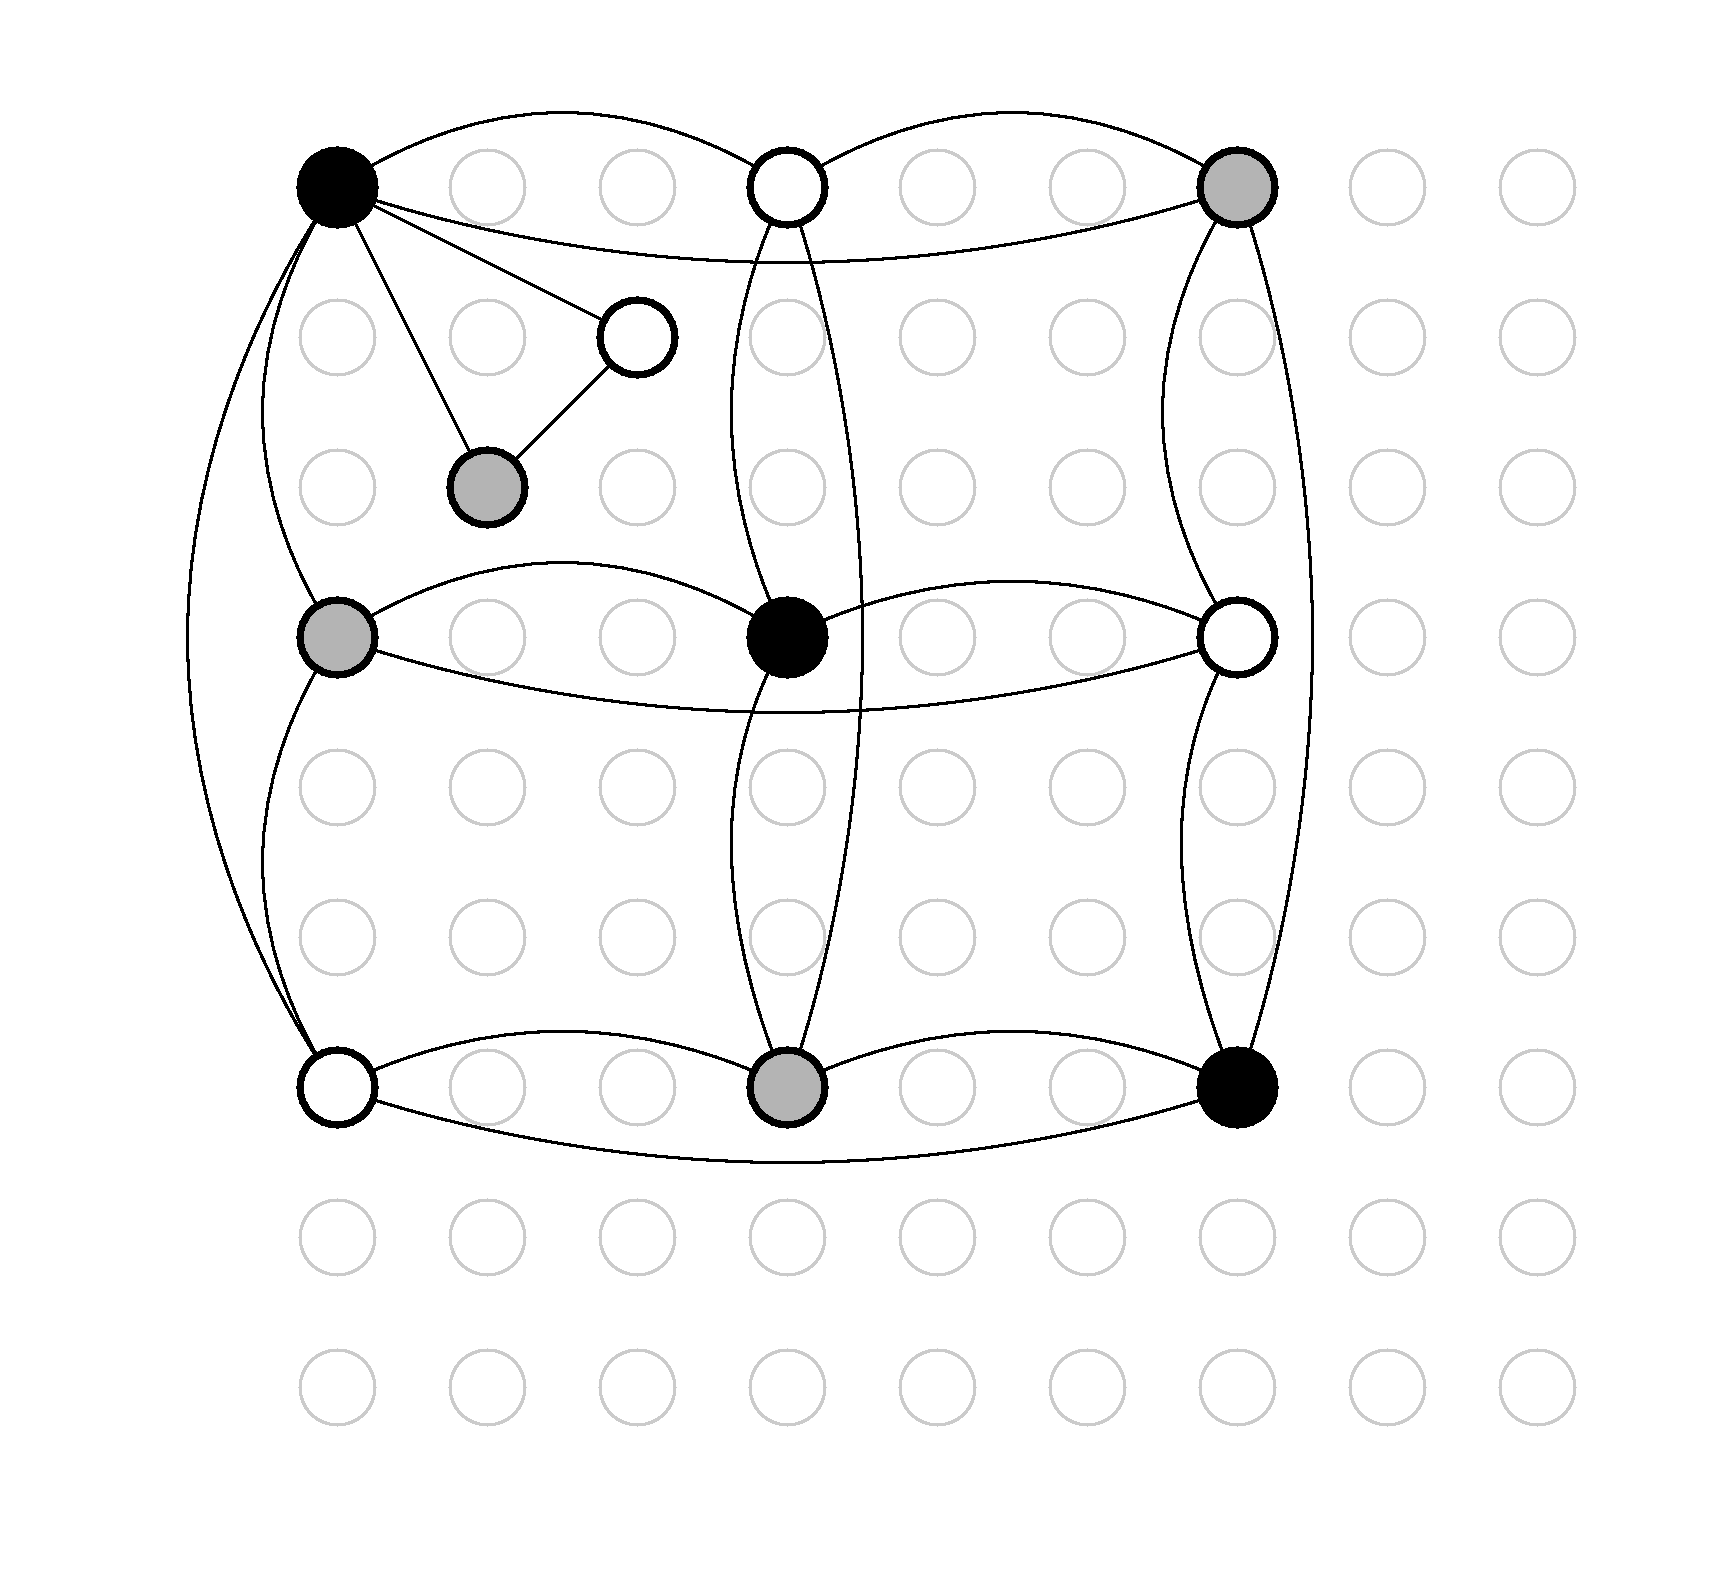
\includegraphics[width=0.5\textwidth]{figs/sudoku-graph-bw}
\caption{A Sudoku game board and the corresponding colored graph.}
\label{fig:sudoku-graph}
\end{figure}

Some techniques for playing Sudoku correspond to heuristics used in
graph coloring algorithms.  For example, one of the basic techniques
for Sudoku is called Pencil Marks. The idea is to use a process of
elimination to determine what numbers are no longer available for a
square and write down those numbers in the square (writing very
small). For example, if the number $1$ is assigned to a square, then
write the pencil mark $1$ in all the squares in the same row, column,
and region to indicate that $1$ is no longer an option for those other
squares.
%
The Pencil Marks technique corresponds to the notion of
\emph{saturation}\index{subject}{saturation} due to \cite{Brelaz:1979eu}.  The
saturation of a vertex, in Sudoku terms, is the set of numbers that
are no longer available. In graph terminology, we have the following
definition:
\begin{equation*}
  \mathrm{saturation}(u) = \{ c \;|\; \exists v. v \in \mathrm{adjacent}(u)
     \text{ and } \mathrm{color}(v) = c \}
\end{equation*}
where $\mathrm{adjacent}(u)$ is the set of vertices that share an
edge with $u$.

The Pencil Marks technique leads to a simple strategy for filling in
numbers: if there is a square with only one possible number left, then
choose that number! But what if there are no squares with only one
possibility left? One brute-force approach is to try them all: choose
the first one and if that ultimately leads to a solution, great.  If
not, backtrack and choose the next possibility.  One good thing about
Pencil Marks is that it reduces the degree of branching in the search
tree. Nevertheless, backtracking can be terribly time consuming. One
way to reduce the amount of backtracking is to use the
most-constrained-first heuristic (aka. minimum remaining
values)~\citep{Russell2003}.  That is, when choosing a square, always
choose one with the fewest possibilities left (the vertex with the
highest saturation).  The idea is that choosing highly constrained
squares earlier rather than later is better because later on there may
not be any possibilities left in the highly saturated squares.

However, register allocation is easier than Sudoku because the
register allocator can fall back to assigning variables to stack
locations when the registers run out. Thus, it makes sense to replace
backtracking with greedy search: make the best choice at the time and
keep going. We still wish to minimize the number of colors needed, so
we use the most-constrained-first heuristic in the greedy search.
Figure~\ref{fig:satur-algo} gives the pseudo-code for a simple greedy
algorithm for register allocation based on saturation and the
most-constrained-first heuristic. It is roughly equivalent to the
DSATUR graph coloring algorithm~\citep{Brelaz:1979eu}.
%,Gebremedhin:1999fk,Omari:2006uq
Just as in Sudoku, the algorithm represents colors with integers. The
integers $0$ through $k-1$ correspond to the $k$ registers that we use
for register allocation. The integers $k$ and larger correspond to
stack locations. The registers that are not used for register
allocation, such as \code{rax}, are assigned to negative integers. In
particular, we assign $-1$ to \code{rax} and $-2$ to \code{rsp}.

%% One might wonder why we include registers at all in the liveness
%% analysis and interference graph. For example, we never allocate a
%% variable to \code{rax} and \code{rsp}, so it would be harmless to
%% leave them out.  As we see in Chapter~\ref{ch:Lvec}, when we begin
%% to use register for passing arguments to functions, it will be
%% necessary for those registers to appear in the interference graph
%% because those registers will also be assigned to variables, and we
%% don't want those two uses to encroach on each other. Regarding
%% registers such as \code{rax} and \code{rsp} that are not used for
%% variables, we could omit them from the interference graph but that
%% would require adding special cases to our algorithm, which would
%% complicate the logic for little gain.


\begin{figure}[btp]
  \centering
\begin{lstlisting}[basicstyle=\rmfamily,deletekeywords={for,from,with,is,not,in,find},morekeywords={while},columns=fullflexible]
Algorithm: DSATUR
Input: a graph |$G$|
Output: an assignment |$\mathrm{color}[v]$| for each vertex |$v \in G$|

|$W \gets \mathrm{vertices}(G)$|
while |$W \neq \emptyset$| do
    pick a vertex |$u$| from |$W$| with the highest saturation,
        breaking ties randomly
    find the lowest color |$c$| that is not in |$\{ \mathrm{color}[v] \;:\; v \in \mathrm{adjacent}(u)\}$|
    |$\mathrm{color}[u] \gets c$|
    |$W \gets W - \{u\}$|
\end{lstlisting}
  \caption{The saturation-based greedy graph coloring algorithm.}
  \label{fig:satur-algo}
\end{figure}

{\if\edition\racketEd      
With the DSATUR algorithm in hand, let us return to the running
example and consider how to color the interference graph in
Figure~\ref{fig:interfere}.
%
We start by assigning the register nodes to their own color. For
example, \code{rax} is assigned the color $-1$ and \code{rsp} is
assigned $-2$.  The variables are not yet colored, so they are
annotated with a dash. We then update the saturation for vertices that
are adjacent to a register, obtaining the following annotated
graph. For example, the saturation for \code{t} is $\{-1,-2\}$ because
it interferes with both \code{rax} and \code{rsp}.
\[
\begin{tikzpicture}[baseline=(current  bounding  box.center)]
\node (rax) at (0,0) {$\ttm{rax}:-1,\{-2\}$};
\node (rsp) at (10,2) {$\ttm{rsp}:-2,\{-1\}$};
\node (t1) at (0,2) {$\ttm{t}:-,\{-1,-2\}$};
\node (z) at (3,2)  {$\ttm{z}:-,\{-2\}$};
\node (x) at (6,2)  {$\ttm{x}:-,\{-2\}$};
\node (y) at (3,0)  {$\ttm{y}:-,\{-2\}$};
\node (w) at (6,0)  {$\ttm{w}:-,\{-2\}$};
\node (v) at (10,0)  {$\ttm{v}:-,\{-2\}$};

\draw (t1) to (rax);
\draw (t1) to (z);
\draw (z) to (y);
\draw (z) to (w);
\draw (x) to (w);
\draw (y) to (w);
\draw (v) to (w);

\draw (v) to (rsp);
\draw (w) to (rsp);
\draw (x) to (rsp);
\draw (y) to (rsp);
\path[-.,bend left=15] (z) edge node {} (rsp);
\path[-.,bend left=10] (t1) edge node {} (rsp);
\draw (rax) to (rsp);
\end{tikzpicture}
\]
The algorithm says to select a maximally saturated vertex. So we pick
$\ttm{t}$ and color it with the first available integer, which is
$0$. We mark $0$ as no longer available for $\ttm{z}$, $\ttm{rax}$,
and \ttm{rsp} because they interfere with $\ttm{t}$.
\[
\begin{tikzpicture}[baseline=(current  bounding  box.center)]
\node (rax) at (0,0) {$\ttm{rax}:-1,\{0,-2\}$};
\node (rsp) at (10,2) {$\ttm{rsp}:-2,\{-1,0\}$};
\node (t1) at (0,2) {$\ttm{t}:0,\{-1,-2\}$};
\node (z) at (3,2)  {$\ttm{z}:-,\{0,-2\}$};
\node (x) at (6,2)  {$\ttm{x}:-,\{-2\}$};
\node (y) at (3,0)  {$\ttm{y}:-,\{-2\}$};
\node (w) at (6,0)  {$\ttm{w}:-,\{-2\}$};
\node (v) at (10,0)  {$\ttm{v}:-,\{-2\}$};

\draw (t1) to (rax);
\draw (t1) to (z);
\draw (z) to (y);
\draw (z) to (w);
\draw (x) to (w);
\draw (y) to (w);
\draw (v) to (w);

\draw (v) to (rsp);
\draw (w) to (rsp);
\draw (x) to (rsp);
\draw (y) to (rsp);
\path[-.,bend left=15] (z) edge node {} (rsp);
\path[-.,bend left=10] (t1) edge node {} (rsp);
\draw (rax) to (rsp);
\end{tikzpicture}
\]
We repeat the process, selecting a maximally saturated vertex,
choosing is \code{z}, and color it with the first available number, which
is $1$. We add $1$ to the saturation for the neighboring vertices
\code{t}, \code{y}, \code{w}, and \code{rsp}.
\[
\begin{tikzpicture}[baseline=(current  bounding  box.center)]
\node (rax) at (0,0) {$\ttm{rax}:-1,\{0,-2\}$};
\node (rsp) at (10,2) {$\ttm{rsp}:-2,\{-1,0,1\}$};
\node (t1) at (0,2) {$\ttm{t}:0,\{-1,1,-2\}$};
\node (z) at (3,2)  {$\ttm{z}:1,\{0,-2\}$};
\node (x) at (6,2)  {$\ttm{x}:-,\{-2\}$};
\node (y) at (3,0)  {$\ttm{y}:-,\{1,-2\}$};
\node (w) at (6,0)  {$\ttm{w}:-,\{1,-2\}$};
\node (v) at (10,0)  {$\ttm{v}:-,\{-2\}$};

\draw (t1) to (rax);
\draw (t1) to (z);
\draw (z) to (y);
\draw (z) to (w);
\draw (x) to (w);
\draw (y) to (w);
\draw (v) to (w);

\draw (v) to (rsp);
\draw (w) to (rsp);
\draw (x) to (rsp);
\draw (y) to (rsp);
\path[-.,bend left=15] (z) edge node {} (rsp);
\path[-.,bend left=10] (t1) edge node {} (rsp);
\draw (rax) to (rsp);
\end{tikzpicture}
\]
The most saturated vertices are now \code{w} and \code{y}. We color
\code{w} with the first available color, which is $0$.
\[
\begin{tikzpicture}[baseline=(current  bounding  box.center)]
\node (rax) at (0,0) {$\ttm{rax}:-1,\{0,-2\}$};
\node (rsp) at (10,2) {$\ttm{rsp}:-2,\{-1,0,1\}$};
\node (t1) at (0,2) {$\ttm{t}:0,\{-1,1,-2\}$};
\node (z) at (3,2)  {$\ttm{z}:1,\{0,-2\}$};
\node (x) at (6,2)  {$\ttm{x}:-,\{0,-2\}$};
\node (y) at (3,0)  {$\ttm{y}:-,\{0,1,-2\}$};
\node (w) at (6,0)  {$\ttm{w}:0,\{1,-2\}$};
\node (v) at (10,0)  {$\ttm{v}:-,\{0,-2\}$};

\draw (t1) to (rax);
\draw (t1) to (z);
\draw (z) to (y);
\draw (z) to (w);
\draw (x) to (w);
\draw (y) to (w);
\draw (v) to (w);

\draw (v) to (rsp);
\draw (w) to (rsp);
\draw (x) to (rsp);
\draw (y) to (rsp);
\path[-.,bend left=15] (z) edge node {} (rsp);
\path[-.,bend left=10] (t1) edge node {} (rsp);
\draw (rax) to (rsp);
\end{tikzpicture}
\]
Vertex \code{y} is now the most highly saturated, so we color \code{y}
with $2$.  We cannot choose $0$ or $1$ because those numbers are in
\code{y}'s saturation set. Indeed, \code{y} interferes with \code{w}
and \code{z}, whose colors are $0$ and $1$ respectively.
\[
\begin{tikzpicture}[baseline=(current  bounding  box.center)]
\node (rax) at (0,0) {$\ttm{rax}:-1,\{0,-2\}$};
\node (rsp) at (10,2) {$\ttm{rsp}:-2,\{-1,0,1,2\}$};
\node (t1) at (0,2) {$\ttm{t}:0,\{-1,1,-2\}$};
\node (z) at (3,2)  {$\ttm{z}:1,\{0,2,-2\}$};
\node (x) at (6,2)  {$\ttm{x}:-,\{0,-2\}$};
\node (y) at (3,0)  {$\ttm{y}:2,\{0,1,-2\}$};
\node (w) at (6,0)  {$\ttm{w}:0,\{1,2,-2\}$};
\node (v) at (10,0)  {$\ttm{v}:-,\{0,-2\}$};

\draw (t1) to (rax);
\draw (t1) to (z);
\draw (z) to (y);
\draw (z) to (w);
\draw (x) to (w);
\draw (y) to (w);
\draw (v) to (w);

\draw (v) to (rsp);
\draw (w) to (rsp);
\draw (x) to (rsp);
\draw (y) to (rsp);
\path[-.,bend left=15] (z) edge node {} (rsp);
\path[-.,bend left=10] (t1) edge node {} (rsp);
\draw (rax) to (rsp);
\end{tikzpicture}
\]
Now \code{x} and \code{v} are the most saturated, so we color \code{v} with $1$.
\[
\begin{tikzpicture}[baseline=(current  bounding  box.center)]
\node (rax) at (0,0) {$\ttm{rax}:-1,\{0,-2\}$};
\node (rsp) at (10,2) {$\ttm{rsp}:-2,\{-1,0,1,2\}$};
\node (t1) at (0,2) {$\ttm{t}:0,\{-1,1,-2\}$};
\node (z) at (3,2)  {$\ttm{z}:1,\{0,2,-2\}$};
\node (x) at (6,2)  {$\ttm{x}:-,\{0,-2\}$};
\node (y) at (3,0)  {$\ttm{y}:2,\{0,1,-2\}$};
\node (w) at (6,0)  {$\ttm{w}:0,\{1,2,-2\}$};
\node (v) at (10,0)  {$\ttm{v}:1,\{0,-2\}$};

\draw (t1) to (rax);
\draw (t1) to (z);
\draw (z) to (y);
\draw (z) to (w);
\draw (x) to (w);
\draw (y) to (w);
\draw (v) to (w);

\draw (v) to (rsp);
\draw (w) to (rsp);
\draw (x) to (rsp);
\draw (y) to (rsp);
\path[-.,bend left=15] (z) edge node {} (rsp);
\path[-.,bend left=10] (t1) edge node {} (rsp);
\draw (rax) to (rsp);
\end{tikzpicture}
\]
In the last step of the algorithm, we color \code{x} with $1$.
\[
\begin{tikzpicture}[baseline=(current  bounding  box.center)]
\node (rax) at (0,0) {$\ttm{rax}:-1,\{0,-2\}$};
\node (rsp) at (10,2) {$\ttm{rsp}:-2,\{-1,0,1,2\}$};
\node (t1) at (0,2) {$\ttm{t}:0,\{-1,1,-2\}$};
\node (z) at (3,2)  {$\ttm{z}:1,\{0,2,-2\}$};
\node (x) at (6,2)  {$\ttm{x}:1,\{0,-2\}$};
\node (y) at (3,0)  {$\ttm{y}:2,\{0,1,-2\}$};
\node (w) at (6,0)  {$\ttm{w}:0,\{1,2,-2\}$};
\node (v) at (10,0)  {$\ttm{v}:1,\{0,-2\}$};

\draw (t1) to (rax);
\draw (t1) to (z);
\draw (z) to (y);
\draw (z) to (w);
\draw (x) to (w);
\draw (y) to (w);
\draw (v) to (w);

\draw (v) to (rsp);
\draw (w) to (rsp);
\draw (x) to (rsp);
\draw (y) to (rsp);
\path[-.,bend left=15] (z) edge node {} (rsp);
\path[-.,bend left=10] (t1) edge node {} (rsp);
\draw (rax) to (rsp);
\end{tikzpicture}
\]
So we obtain the following coloring:
\[
\{
\ttm{rax} \mapsto -1,
\ttm{rsp} \mapsto -2,
\ttm{t} \mapsto 0,
\ttm{z} \mapsto 1,
\ttm{x} \mapsto 1,
\ttm{y} \mapsto 2,
\ttm{w} \mapsto 0,
\ttm{v} \mapsto 1
\}
\]
\fi}
%
{\if\edition\pythonEd
%
With the DSATUR algorithm in hand, let us return to the running
example and consider how to color the interference graph in
Figure~\ref{fig:interfere}. We annotate each variable node with a dash
to indicate that it has not yet been assigned a color. The saturation
sets are also shown for each node; all of them start as the empty set.
(We do not include the register nodes in the graph below because there
were no interference edges involving registers in this program, but in
general there can be.)
%
\[
\begin{tikzpicture}[baseline=(current  bounding  box.center)]
\node (t0) at (0,2) {$\ttm{tmp\_0}: -, \{\}$};
\node (t1) at (0,0) {$\ttm{tmp\_1}: -, \{\}$};
\node (z) at (3,2)  {$\ttm{z}: -, \{\}$};
\node (x) at (6,2)  {$\ttm{x}: -, \{\}$};
\node (y) at (3,0)  {$\ttm{y}: -, \{\}$};
\node (w) at (6,0)  {$\ttm{w}: -, \{\}$};
\node (v) at (9,0)  {$\ttm{v}: -, \{\}$};

\draw (t0) to (t1);
\draw (t0) to (z);
\draw (z) to (y);
\draw (z) to (w);
\draw (x) to (w);
\draw (y) to (w);
\draw (v) to (w);
\end{tikzpicture}
\]
The algorithm says to select a maximally saturated vertex, but they
are all equally saturated. So we flip a coin and pick $\ttm{tmp\_0}$
then color it with the first available integer, which is $0$. We mark
$0$ as no longer available for $\ttm{tmp\_1}$ and $\ttm{z}$ because
they interfere with $\ttm{tmp\_0}$.
\[
\begin{tikzpicture}[baseline=(current  bounding  box.center)]
\node (t0) at (0,2) {$\ttm{tmp\_0}: 0, \{\}$};
\node (t1) at (0,0) {$\ttm{tmp\_1}: -, \{0\}$};
\node (z) at (3,2)  {$\ttm{z}: -, \{0\}$};
\node (x) at (6,2)  {$\ttm{x}: -, \{\}$};
\node (y) at (3,0)  {$\ttm{y}: -, \{\}$};
\node (w) at (6,0)  {$\ttm{w}: -, \{\}$};
\node (v) at (9,0)  {$\ttm{v}: -, \{\}$};

\draw (t0) to (t1);
\draw (t0) to (z);
\draw (z) to (y);
\draw (z) to (w);
\draw (x) to (w);
\draw (y) to (w);
\draw (v) to (w);
\end{tikzpicture}
\]
We repeat the process. The most saturated vertices are \code{z} and
\code{tmp\_1}, so we choose \code{z} and color it with the first
available number, which is $1$. We add $1$ to the saturation for the
neighboring vertices \code{tmp\_0}, \code{y}, and \code{w}.
\[
\begin{tikzpicture}[baseline=(current  bounding  box.center)]
\node (t0) at (0,2) {$\ttm{tmp\_0}: 0, \{1\}$};
\node (t1) at (0,0) {$\ttm{tmp\_1}: -, \{0\}$};
\node (z) at (3,2)  {$\ttm{z}: 1, \{0\}$};
\node (x) at (6,2)  {$\ttm{x}: -, \{\}$};
\node (y) at (3,0)  {$\ttm{y}: -, \{1\}$};
\node (w) at (6,0)  {$\ttm{w}: -, \{1\}$};
\node (v) at (9,0)  {$\ttm{v}: -, \{\}$};

\draw (t0) to (t1);
\draw (t0) to (z);
\draw (z) to (y);
\draw (z) to (w);
\draw (x) to (w);
\draw (y) to (w);
\draw (v) to (w);
\end{tikzpicture}
\]
The most saturated vertices are now \code{tmp\_1}, \code{w}, and
\code{y}. We color \code{w} with the first available color, which
is $0$.
\[
\begin{tikzpicture}[baseline=(current  bounding  box.center)]
\node (t0) at (0,2) {$\ttm{tmp\_0}: 0, \{1\}$};
\node (t1) at (0,0) {$\ttm{tmp\_1}: -, \{0\}$};
\node (z) at (3,2)  {$\ttm{z}: 1, \{0\}$};
\node (x) at (6,2)  {$\ttm{x}: -, \{0\}$};
\node (y) at (3,0)  {$\ttm{y}: -, \{0,1\}$};
\node (w) at (6,0)  {$\ttm{w}: 0, \{1\}$};
\node (v) at (9,0)  {$\ttm{v}: -, \{0\}$};

\draw (t0) to (t1);
\draw (t0) to (z);
\draw (z) to (y);
\draw (z) to (w);
\draw (x) to (w);
\draw (y) to (w);
\draw (v) to (w);
\end{tikzpicture}
\]
Now \code{y} is the most saturated, so we color it with $2$.
\[
\begin{tikzpicture}[baseline=(current  bounding  box.center)]
\node (t0) at (0,2) {$\ttm{tmp\_0}: 0, \{1\}$};
\node (t1) at (0,0) {$\ttm{tmp\_1}: -, \{0\}$};
\node (z) at (3,2)  {$\ttm{z}: 1, \{0,2\}$};
\node (x) at (6,2)  {$\ttm{x}: -, \{0\}$};
\node (y) at (3,0)  {$\ttm{y}: 2, \{0,1\}$};
\node (w) at (6,0)  {$\ttm{w}: 0, \{1,2\}$};
\node (v) at (9,0)  {$\ttm{v}: -, \{0\}$};

\draw (t0) to (t1);
\draw (t0) to (z);
\draw (z) to (y);
\draw (z) to (w);
\draw (x) to (w);
\draw (y) to (w);
\draw (v) to (w);
\end{tikzpicture}
\]
The most saturated vertices are \code{tmp\_1}, \code{x}, and \code{v}.
We choose to color \code{v} with $1$.
\[
\begin{tikzpicture}[baseline=(current  bounding  box.center)]
\node (t0) at (0,2) {$\ttm{tmp\_0}: 0, \{1\}$};
\node (t1) at (0,0) {$\ttm{tmp\_1}: -, \{0\}$};
\node (z) at (3,2)  {$\ttm{z}: 1, \{0,2\}$};
\node (x) at (6,2)  {$\ttm{x}: -, \{0\}$};
\node (y) at (3,0)  {$\ttm{y}: 2, \{0,1\}$};
\node (w) at (6,0)  {$\ttm{w}: 0, \{1,2\}$};
\node (v) at (9,0)  {$\ttm{v}: 1, \{0\}$};

\draw (t0) to (t1);
\draw (t0) to (z);
\draw (z) to (y);
\draw (z) to (w);
\draw (x) to (w);
\draw (y) to (w);
\draw (v) to (w);
\end{tikzpicture}
\]
We color the remaining two variables, \code{tmp\_1} and \code{x}, with $1$.
\[
\begin{tikzpicture}[baseline=(current  bounding  box.center)]
\node (t0) at (0,2) {$\ttm{tmp\_0}: 0, \{1\}$};
\node (t1) at (0,0) {$\ttm{tmp\_1}: 1, \{0\}$};
\node (z) at (3,2)  {$\ttm{z}: 1, \{0,2\}$};
\node (x) at (6,2)  {$\ttm{x}: 1, \{0\}$};
\node (y) at (3,0)  {$\ttm{y}: 2, \{0,1\}$};
\node (w) at (6,0)  {$\ttm{w}: 0, \{1,2\}$};
\node (v) at (9,0)  {$\ttm{v}: 1, \{0\}$};

\draw (t0) to (t1);
\draw (t0) to (z);
\draw (z) to (y);
\draw (z) to (w);
\draw (x) to (w);
\draw (y) to (w);
\draw (v) to (w);
\end{tikzpicture}
\]
So we obtain the following coloring:
\[
\{ \ttm{tmp\_0} \mapsto  0, 
   \ttm{tmp\_1} \mapsto  1, 
   \ttm{z} \mapsto  1,
   \ttm{x} \mapsto  1,
   \ttm{y} \mapsto  2,
   \ttm{w} \mapsto  0, 
   \ttm{v} \mapsto  1 \}
\]
\fi}

We recommend creating an auxiliary function named \code{color\_graph}
that takes an interference graph and a list of all the variables in
the program. This function should return a mapping of variables to
their colors (represented as natural numbers). By creating this helper
function, you will be able to reuse it in Chapter~\ref{ch:Lfun}
when we add support for functions.

To prioritize the processing of highly saturated nodes inside the
\code{color\_graph} function, we recommend using the priority queue
data structure \racket{described in Figure~\ref{fig:priority-queue}}\python{in the file \code{priority\_queue.py} of the support code}. \racket{In
addition, you will need to maintain a mapping from variables to their
``handles'' in the priority queue so that you can notify the priority
queue when their saturation changes.}

{\if\edition\racketEd      
\begin{figure}[tp]
%\begin{wrapfigure}[25]{r}[0.75in]{0.55\textwidth}
  \small
  \begin{tcolorbox}[title=Priority Queue]
    A \emph{priority queue} is a collection of items in which the
    removal of items is governed by priority. In a ``min'' queue,
    lower priority items are removed first. An implementation is in
    \code{priority\_queue.rkt} of the support code.  \index{subject}{priority
      queue} \index{subject}{minimum priority queue}
  \begin{description}
  \item[$\LP\code{make-pqueue}\,\itm{cmp}\RP$] constructs an empty
    priority queue that uses the $\itm{cmp}$ predicate to determine
    whether its first argument has lower or equal priority to its
    second argument.
  \item[$\LP\code{pqueue-count}\,\itm{queue}\RP$] returns the number of
    items in the queue.
  \item[$\LP\code{pqueue-push!}\,\itm{queue}\,\itm{item}\RP$] inserts
    the item into the queue and returns a handle for the item in the
    queue.
  \item[$\LP\code{pqueue-pop!}\,\itm{queue}\RP$] returns the item with
    the lowest priority.
  \item[$\LP\code{pqueue-decrease-key!}\,\itm{queue}\,\itm{handle}\RP$]
    notifies the queue that the priority has decreased for the item
    associated with the given handle.
  \end{description}
\end{tcolorbox}
  %\end{wrapfigure}
  \caption{The priority queue data structure.}
  \label{fig:priority-queue}
\end{figure}
\fi}

With the coloring complete, we finalize the assignment of variables to
registers and stack locations. We map the first $k$ colors to the $k$
registers and the rest of the colors to stack locations.  Suppose for
the moment that we have just one register to use for register
allocation, \key{rcx}. Then we have the following map from colors to
locations.
\[
  \{ 0 \mapsto \key{\%rcx}, \; 1 \mapsto \key{-8(\%rbp)}, \; 2 \mapsto \key{-16(\%rbp)} \}
\]
Composing this mapping with the coloring, we arrive at the following
assignment of variables to locations.
{\if\edition\racketEd      
\begin{gather*}
  \{ \ttm{v} \mapsto \key{-8(\%rbp)}, \,
     \ttm{w} \mapsto \key{\%rcx},  \,
     \ttm{x} \mapsto \key{-8(\%rbp)}, \,
     \ttm{y} \mapsto \key{-16(\%rbp)}, \\
     \ttm{z} \mapsto \key{-8(\%rbp)}, \,
     \ttm{t} \mapsto \key{\%rcx} \}
\end{gather*}
\fi}
{\if\edition\pythonEd
\begin{gather*}
  \{ \ttm{v} \mapsto \key{-8(\%rbp)},  \,
     \ttm{w} \mapsto \key{\%rcx}, \,
     \ttm{x} \mapsto \key{-8(\%rbp)}, \,
     \ttm{y} \mapsto \key{-16(\%rbp)}, \\
     \ttm{z} \mapsto \key{-8(\%rbp)}, \,
     \ttm{tmp\_0} \mapsto \key{\%rcx}, \,
     \ttm{tmp\_1} \mapsto \key{-8(\%rbp)} \}
\end{gather*}
\fi}

Adapt the code from the \code{assign\_homes} pass
(Section~\ref{sec:assign-Lvar}) to replace the variables with their
assigned location. Applying the above assignment to our running
example, on the left, yields the program on the right.
% why frame size of 32? -JGS
\begin{center}
{\if\edition\racketEd      
\begin{minipage}{0.3\textwidth}
\begin{lstlisting}
movq $1, v
movq $42, w
movq v, x
addq $7, x
movq x, y
movq x, z
addq w, z
movq y, t
negq t
movq z, %rax
addq t, %rax
jmp conclusion
\end{lstlisting}
\end{minipage}
$\Rightarrow\qquad$
\begin{minipage}{0.45\textwidth}
\begin{lstlisting}
movq $1, -8(%rbp)
movq $42, %rcx
movq -8(%rbp), -8(%rbp)
addq $7, -8(%rbp)
movq -8(%rbp), -16(%rbp)
movq -8(%rbp), -8(%rbp)
addq %rcx, -8(%rbp)
movq -16(%rbp), %rcx
negq %rcx
movq -8(%rbp), %rax
addq %rcx, %rax
jmp conclusion
\end{lstlisting}
\end{minipage}
\fi}
{\if\edition\pythonEd
\begin{minipage}{0.3\textwidth}
\begin{lstlisting}
movq $1, v
movq $42, w
movq v, x
addq $7, x
movq x, y
movq x, z
addq w, z
movq y, tmp_0
negq tmp_0
movq z, tmp_1
addq tmp_0, tmp_1
movq tmp_1, %rdi
callq print_int
\end{lstlisting}
\end{minipage}
$\Rightarrow\qquad$
\begin{minipage}{0.45\textwidth}
\begin{lstlisting}
movq $1, -8(%rbp)
movq $42, %rcx
movq -8(%rbp), -8(%rbp)
addq $7, -8(%rbp)
movq -8(%rbp), -16(%rbp)
movq -8(%rbp), -8(%rbp)
addq %rcx, -8(%rbp)
movq -16(%rbp), %rcx
negq %rcx
movq -8(%rbp), -8(%rbp)
addq %rcx, -8(%rbp)
movq -8(%rbp), %rdi
callq print_int    
\end{lstlisting}
\end{minipage}
\fi}
\end{center}

\begin{exercise}\normalfont\normalsize
%
Implement the compiler pass \code{allocate\_registers}.
%
Create five programs that exercise all aspects of the register
allocation algorithm, including spilling variables to the stack.
%
\racket{Replace \code{assign\_homes} in the list of \code{passes} in the
\code{run-tests.rkt} script with the three new passes:
\code{uncover\_live}, \code{build\_interference}, and
\code{allocate\_registers}.
%
Temporarily remove the \code{print\_x86} pass from the list of passes
and the call to \code{compiler-tests}.
Run the script to test the register allocator.
}
%
\python{Run the \code{run-tests.py} script to to check whether the
  output programs produce the same result as the input programs.}
\end{exercise}


\section{Patch Instructions}
\label{sec:patch-instructions}

The remaining step in the compilation to x86 is to ensure that the
instructions have at most one argument that is a memory access.
%
In the running example, the instruction \code{movq -8(\%rbp),
    -16(\%rbp)} is problematic. Recall from Section~\ref{sec:patch-s0}
  that the fix is to first move \code{-8(\%rbp)} into \code{rax} and
  then move \code{rax} into \code{-16(\%rbp)}.
%
The moves from \code{-8(\%rbp)} to \code{-8(\%rbp)} are also
problematic, but they can simply be deleted. In general, we recommend
deleting all the trivial moves whose source and destination are the
same location.
%
The following is the output of \code{patch\_instructions} on the
running example.
\begin{center}
{\if\edition\racketEd      
\begin{minipage}{0.4\textwidth}
\begin{lstlisting}
movq $1, -8(%rbp)
movq $42, %rcx
movq -8(%rbp), -8(%rbp)
addq $7, -8(%rbp)
movq -8(%rbp), -16(%rbp)
movq -8(%rbp), -8(%rbp)
addq %rcx, -8(%rbp)
movq -16(%rbp), %rcx
negq %rcx
movq -8(%rbp), %rax
addq %rcx, %rax
jmp conclusion
\end{lstlisting}
\end{minipage}
$\Rightarrow\qquad$
\begin{minipage}{0.45\textwidth}
\begin{lstlisting}
movq $1, -8(%rbp)
movq $42, %rcx
addq $7, -8(%rbp)
movq -8(%rbp), %rax
movq %rax, -16(%rbp)
addq %rcx, -8(%rbp)
movq -16(%rbp), %rcx
negq %rcx
movq -8(%rbp), %rax
addq %rcx, %rax
jmp conclusion
\end{lstlisting}
\end{minipage}
\fi}
{\if\edition\pythonEd
\begin{minipage}{0.4\textwidth}
\begin{lstlisting}
movq $1, -8(%rbp)
movq $42, %rcx
movq -8(%rbp), -8(%rbp)
addq $7, -8(%rbp)
movq -8(%rbp), -16(%rbp)
movq -8(%rbp), -8(%rbp)
addq %rcx, -8(%rbp)
movq -16(%rbp), %rcx
negq %rcx
movq -8(%rbp), -8(%rbp)
addq %rcx, -8(%rbp)
movq -8(%rbp), %rdi
callq print_int    
\end{lstlisting}
\end{minipage}
$\Rightarrow\qquad$
\begin{minipage}{0.45\textwidth}
\begin{lstlisting}
movq $1, -8(%rbp)
movq $42, %rcx
addq $7, -8(%rbp)
movq -8(%rbp), %rax
movq %rax, -16(%rbp)
addq %rcx, -8(%rbp)
movq -16(%rbp), %rcx
negq %rcx
addq %rcx, -8(%rbp)
movq -8(%rbp), %rdi
callq print_int    
\end{lstlisting}
\end{minipage}
\fi}
\end{center}

\begin{exercise}\normalfont\normalsize
%
Update the \code{patch\_instructions} compiler pass to delete trivial moves.
%
%Insert it after \code{allocate\_registers} in the list of \code{passes}
%in the \code{run-tests.rkt} script.
%
Run the script to test the \code{patch\_instructions} pass.
\end{exercise}


\section{Prelude and Conclusion}
\label{sec:print-x86-reg-alloc}
\index{subject}{calling conventions}
\index{subject}{prelude}\index{subject}{conclusion}

Recall that this pass generates the prelude and conclusion
instructions to satisfy the x86 calling conventions
(Section~\ref{sec:calling-conventions}). With the addition of the
register allocator, the callee-saved registers used by the register
allocator must be saved in the prelude and restored in the conclusion.
In the \code{allocate\_registers} pass,
%
\racket{add an entry to the \itm{info}
  of \code{X86Program} named \code{used\_callee}}
%
\python{add a field named \code{used\_callee} to the \code{X86Program} AST node}
%
that stores the set of callee-saved registers that were assigned to
variables. The \code{prelude\_and\_conclusion} pass can then access
this information to decide which callee-saved registers need to be
saved and restored.
%
When calculating the size of the frame to adjust the \code{rsp} in the
prelude, make sure to take into account the space used for saving the
callee-saved registers. Also, don't forget that the frame needs to be
a multiple of 16 bytes!

\racket{An overview of all of the passes involved in register
  allocation is shown in Figure~\ref{fig:reg-alloc-passes}.}

{\if\edition\racketEd      
\begin{figure}[tbp]
\begin{tikzpicture}[baseline=(current  bounding  box.center)]
\node (Lvar) at (0,2)  {\large \LangVar{}};
\node (Lvar-2) at (3,2)  {\large \LangVar{}};
\node (Lvar-3) at (6,2)  {\large \LangVarANF{}};
\node (Cvar-1) at (3,0)  {\large \LangCVar{}};

\node (x86-2) at (3,-2)  {\large \LangXVar{}};
\node (x86-3) at (6,-2)  {\large \LangXVar{}};
\node (x86-4) at (9,-2) {\large \LangXInt{}};
\node (x86-5) at (9,-4) {\large \LangXInt{}};

\node (x86-2-1) at (3,-4)  {\large \LangXVar{}};
\node (x86-2-2) at (6,-4)  {\large \LangXVar{}};

\path[->,bend left=15] (Lvar) edge [above] node {\ttfamily\footnotesize uniquify} (Lvar-2);
\path[->,bend left=15] (Lvar-2) edge [above] node {\ttfamily\footnotesize remove\_complex.} (Lvar-3);
\path[->,bend left=15] (Lvar-3) edge [right] node {\ttfamily\footnotesize explicate\_control} (Cvar-1);
\path[->,bend right=15] (Cvar-1) edge [left] node {\ttfamily\footnotesize select\_instr.} (x86-2);
\path[->,bend left=15] (x86-2) edge [right] node {\ttfamily\footnotesize uncover\_live} (x86-2-1);
\path[->,bend right=15] (x86-2-1) edge [below] node {\ttfamily\footnotesize build\_inter.} (x86-2-2);
\path[->,bend right=15] (x86-2-2) edge [right] node {\ttfamily\footnotesize allocate\_reg.} (x86-3);
\path[->,bend left=15] (x86-3) edge [above] node {\ttfamily\footnotesize patch\_instr.} (x86-4);
\path[->,bend left=15] (x86-4) edge [right] node {\ttfamily\footnotesize prelude\_and\_concl.} (x86-5);
\end{tikzpicture}
\caption{Diagram of the passes for \LangVar{} with register allocation.}
\label{fig:reg-alloc-passes}
\end{figure}
\fi}

Figure~\ref{fig:running-example-x86} shows the x86 code generated for
the running example (Figure~\ref{fig:reg-eg}). To demonstrate both the
use of registers and the stack, we limit the register allocator for
this example to use just two registers: \code{rbx} and \code{rcx}.  In
the prelude\index{subject}{prelude} of the \code{main} function, we
push \code{rbx} onto the stack because it is a callee-saved register
and it was assigned to variable by the register allocator.  We
subtract \code{8} from the \code{rsp} at the end of the prelude to
reserve space for the one spilled variable.  After that subtraction,
the \code{rsp} is aligned to 16 bytes.

Moving on to the program proper, we see how the registers were
allocated.
%
\racket{Variables \code{v}, \code{x}, and \code{y} were assigned to
  \code{rbx} and variable \code{z} was assigned to \code{rcx}.}
%
\python{Variables \code{v}, \code{x}, \code{y}, and \code{tmp\_0}
  were assigned to \code{rcx} and variables \code{w} and \code{tmp\_1}
  were assigned to \code{rbx}.}
%
Variable \racket{\code{w}}\python{\code{z}} was spilled to the stack
location \code{-16(\%rbp)}.  Recall that the prelude saved the
callee-save register \code{rbx} onto the stack. The spilled variables
must be placed lower on the stack than the saved callee-save
registers, so in this case \racket{\code{w}}\python{z} is placed at
\code{-16(\%rbp)}.

In the conclusion\index{subject}{conclusion}, we undo the work that was
done in the prelude. We move the stack pointer up by \code{8} bytes
(the room for spilled variables), then we pop the old values of
\code{rbx} and \code{rbp} (callee-saved registers), and finish with
\code{retq} to return control to the operating system.

  
\begin{figure}[tbp]
  % var_test_28.rkt
  % (use-minimal-set-of-registers! #t)
  % and only rbx rcx
% tmp 0 rbx
% z 1  rcx
% y 0  rbx
% w 2  16(%rbp)
% v 0  rbx
% x 0  rbx
{\if\edition\racketEd
\begin{lstlisting}
start:
	movq	$1, %rbx
	movq	$42, -16(%rbp)
	addq	$7, %rbx
	movq	%rbx, %rcx
	addq	-16(%rbp), %rcx
	negq	%rbx
	movq	%rcx, %rax
	addq	%rbx, %rax
	jmp conclusion

	.globl main
main:
	pushq	%rbp
	movq	%rsp, %rbp
	pushq	%rbx
	subq	$8, %rsp
	jmp start
        
conclusion:
	addq	$8, %rsp
	popq	%rbx
	popq	%rbp
	retq
\end{lstlisting}
\fi}
{\if\edition\pythonEd
%{v: %rcx, x: %rcx, z: -16(%rbp), w: %rbx, tmp_1: %rbx, y: %rcx, tmp_0: %rcx}  
\begin{lstlisting}
	.globl main
main:
	pushq %rbp
	movq %rsp, %rbp
	pushq %rbx
	subq $8, %rsp
	movq $1, %rcx
	movq $42, %rbx
	addq $7, %rcx
	movq %rcx, -16(%rbp)
	addq %rbx, -16(%rbp)
	negq %rcx
	movq -16(%rbp), %rbx
	addq %rcx, %rbx
	movq %rbx, %rdi
	callq print_int
	addq $8, %rsp
	popq %rbx
	popq %rbp
	retq
\end{lstlisting}
\fi}
\caption{The x86 output from the running example
  (Figure~\ref{fig:reg-eg}), limiting allocation to just \code{rbx}
  and \code{rcx}.}
\label{fig:running-example-x86}
\end{figure}

\begin{exercise}\normalfont\normalsize
Update the \code{prelude\_and\_conclusion} pass as described in this section.
%
\racket{
In the \code{run-tests.rkt} script, add \code{prelude\_and\_conclusion} to the
list of passes and the call to \code{compiler-tests}.}
%
Run the script to test the complete compiler for \LangVar{} that
performs register allocation.
\end{exercise}

\section{Challenge: Move Biasing}
\label{sec:move-biasing}
\index{subject}{move biasing}

This section describes an enhancement to the register allocator,
called move biasing, for students who are looking for an extra
challenge.

{\if\edition\racketEd      
To motivate the need for move biasing we return to the running example
but this time use all of the general purpose registers.  So we have
the following mapping of color numbers to registers.
\[
  \{ 0 \mapsto \key{\%rcx}, \; 1 \mapsto \key{\%rdx}, \; 2 \mapsto \key{\%rsi} \}
\]
Using the same assignment of variables to color numbers that was
produced by the register allocator described in the last section, we
get the following program.
\begin{center}
\begin{minipage}{0.3\textwidth}
\begin{lstlisting}
movq $1, v
movq $42, w
movq v, x
addq $7, x
movq x, y
movq x, z
addq w, z
movq y, t
negq t
movq z, %rax
addq t, %rax
jmp conclusion
\end{lstlisting}
\end{minipage}
$\Rightarrow\qquad$
\begin{minipage}{0.45\textwidth}
\begin{lstlisting}
movq $1, %rdx
movq $42, %rcx
movq %rdx, %rdx
addq $7, %rdx
movq %rdx, %rsi
movq %rdx, %rdx
addq %rcx, %rdx
movq %rsi, %rcx
negq %rcx
movq %rdx, %rax
addq %rcx, %rax
jmp conclusion
\end{lstlisting}
\end{minipage}
\end{center}
In the above output code there are two \key{movq} instructions that
can be removed because their source and target are the same.  However,
if we had put \key{t}, \key{v}, \key{x}, and \key{y} into the same
register, we could instead remove three \key{movq} instructions.  We
can accomplish this by taking into account which variables appear in
\key{movq} instructions with which other variables.
\fi}

{\if\edition\pythonEd
%
To motivate the need for move biasing we return to the running example
and recall that in Section~\ref{sec:patch-instructions} we were able to
remove three trivial move instructions from the running
example. However, we could remove another trivial move if we were able
to allocate \code{y} and \code{tmp\_0} to the same register.  \fi}

We say that two variables $p$ and $q$ are \emph{move
related}\index{subject}{move related} if they participate together in
a \key{movq} instruction, that is, \key{movq} $p$\key{,} $q$ or
\key{movq} $q$\key{,} $p$. When deciding which variable to color next,
when there are multiple variables with the same saturation, prefer
variables that can be assigned to a color that is the same as the
color of a move related variable.  Furthermore, when the register
allocator chooses a color for a variable, it should prefer a color
that has already been used for a move-related variable (assuming that
they do not interfere). Of course, this preference should not override
the preference for registers over stack locations. So this preference
should be used as a tie breaker when choosing between registers or
when choosing between stack locations.

We recommend representing the move relationships in a graph, similar
to how we represented interference.  The following is the \emph{move
  graph} for our running example.
{\if\edition\racketEd      
\[
\begin{tikzpicture}[baseline=(current  bounding  box.center)]
\node (rax) at (0,0) {$\ttm{rax}$};
\node (rsp) at (9,2) {$\ttm{rsp}$};
\node (t) at (0,2) {$\ttm{t}$};
\node (z) at (3,2)  {$\ttm{z}$};
\node (x) at (6,2)  {$\ttm{x}$};
\node (y) at (3,0)  {$\ttm{y}$};
\node (w) at (6,0)  {$\ttm{w}$};
\node (v) at (9,0)  {$\ttm{v}$};

\draw (v) to (x);
\draw (x) to (y);
\draw (x) to (z);
\draw (y) to (t);
\end{tikzpicture}
\]
\fi}
%
{\if\edition\pythonEd
\[
\begin{tikzpicture}[baseline=(current  bounding  box.center)]
\node (t0) at (0,2) {$\ttm{tmp\_0}$};
\node (t1) at (0,0) {$\ttm{tmp\_1}$};
\node (z) at (3,2)  {$\ttm{z}$};
\node (x) at (6,2)  {$\ttm{x}$};
\node (y) at (3,0)  {$\ttm{y}$};
\node (w) at (6,0)  {$\ttm{w}$};
\node (v) at (9,0)  {$\ttm{v}$};

\draw (y) to (t0);
\draw (z) to (x);
\draw (z) to (t1);
\draw (x) to (y);
\draw (x) to (v);
\end{tikzpicture}
\]
\fi}

{\if\edition\racketEd
Now we replay the graph coloring, pausing to see the coloring of
\code{y}. Recall the following configuration. The most saturated vertices
were \code{w} and \code{y}.
\[
\begin{tikzpicture}[baseline=(current  bounding  box.center)]
\node (rax) at (0,0) {$\ttm{rax}:-1,\{0,-2\}$};
\node (rsp) at (9,2) {$\ttm{rsp}:-2,\{-1,0,1,2\}$};
\node (t1) at (0,2) {$\ttm{t}:0,\{1,-2\}$};
\node (z) at (3,2)  {$\ttm{z}:1,\{0,-2\}$};
\node (x) at (6,2)  {$\ttm{x}:-,\{-2\}$};
\node (y) at (3,0)  {$\ttm{y}:-,\{1,-2\}$};
\node (w) at (6,0)  {$\ttm{w}:-,\{1,-2\}$};
\node (v) at (9,0)  {$\ttm{v}:-,\{-2\}$};

\draw (t1) to (rax);
\draw (t1) to (z);
\draw (z) to (y);
\draw (z) to (w);
\draw (x) to (w);
\draw (y) to (w);
\draw (v) to (w);

\draw (v) to (rsp);
\draw (w) to (rsp);
\draw (x) to (rsp);
\draw (y) to (rsp);
\path[-.,bend left=15] (z) edge node {} (rsp);
\path[-.,bend left=10] (t1) edge node {} (rsp);
\draw (rax) to (rsp);
\end{tikzpicture}
\]
%
Last time we chose to color \code{w} with $0$. But this time we see
that \code{w} is not move related to any vertex, but \code{y} is move
related to \code{t}.  So we choose to color \code{y} the same color as
\code{t}, $0$.
\[
\begin{tikzpicture}[baseline=(current  bounding  box.center)]
\node (rax) at (0,0) {$\ttm{rax}:-1,\{0,-2\}$};
\node (rsp) at (9,2) {$\ttm{rsp}:-2,\{-1,0,1,2\}$};
\node (t1) at (0,2) {$\ttm{t}:0,\{1,-2\}$};
\node (z) at (3,2)  {$\ttm{z}:1,\{0,-2\}$};
\node (x) at (6,2)  {$\ttm{x}:-,\{-2\}$};
\node (y) at (3,0)  {$\ttm{y}:0,\{1,-2\}$};
\node (w) at (6,0)  {$\ttm{w}:-,\{0,1,-2\}$};
\node (v) at (9,0)  {$\ttm{v}:-,\{-2\}$};

\draw (t1) to (rax);
\draw (t1) to (z);
\draw (z) to (y);
\draw (z) to (w);
\draw (x) to (w);
\draw (y) to (w);
\draw (v) to (w);

\draw (v) to (rsp);
\draw (w) to (rsp);
\draw (x) to (rsp);
\draw (y) to (rsp);
\path[-.,bend left=15] (z) edge node {} (rsp);
\path[-.,bend left=10] (t1) edge node {} (rsp);
\draw (rax) to (rsp);
\end{tikzpicture}
\]
Now \code{w} is the most saturated, so we color it $2$.
\[
\begin{tikzpicture}[baseline=(current  bounding  box.center)]
\node (rax) at (0,0) {$\ttm{rax}:-1,\{0,-2\}$};
\node (rsp) at (9,2) {$\ttm{rsp}:-2,\{-1,0,1,2\}$};
\node (t1) at (0,2) {$\ttm{t}:0,\{1,-2\}$};
\node (z) at (3,2)  {$\ttm{z}:1,\{0,2,-2\}$};
\node (x) at (6,2)  {$\ttm{x}:-,\{2,-2\}$};
\node (y) at (3,0)  {$\ttm{y}:0,\{1,2,-2\}$};
\node (w) at (6,0)  {$\ttm{w}:2,\{0,1,-2\}$};
\node (v) at (9,0)  {$\ttm{v}:-,\{2,-2\}$};

\draw (t1) to (rax);
\draw (t1) to (z);
\draw (z) to (y);
\draw (z) to (w);
\draw (x) to (w);
\draw (y) to (w);
\draw (v) to (w);

\draw (v) to (rsp);
\draw (w) to (rsp);
\draw (x) to (rsp);
\draw (y) to (rsp);
\path[-.,bend left=15] (z) edge node {} (rsp);
\path[-.,bend left=10] (t1) edge node {} (rsp);
\draw (rax) to (rsp);
\end{tikzpicture}
\]
At this point, vertices \code{x} and \code{v} are most saturated, but
\code{x} is move related to \code{y} and \code{z}, so we color
\code{x} to $0$ to match \code{y}. Finally, we color \code{v} to $0$.
\[
\begin{tikzpicture}[baseline=(current  bounding  box.center)]
\node (rax) at (0,0) {$\ttm{rax}:-1,\{0,-2\}$};
\node (rsp) at (9,2) {$\ttm{rsp}:-2,\{-1,0,1,2\}$};
\node (t) at (0,2) {$\ttm{t}:0,\{1,-2\}$};
\node (z) at (3,2)  {$\ttm{z}:1,\{0,2,-2\}$};
\node (x) at (6,2)  {$\ttm{x}:0,\{2,-2\}$};
\node (y) at (3,0)  {$\ttm{y}:0,\{1,2,-2\}$};
\node (w) at (6,0)  {$\ttm{w}:2,\{0,1,-2\}$};
\node (v) at (9,0)  {$\ttm{v}:0,\{2,-2\}$};

\draw (t1) to (rax);
\draw (t) to (z);
\draw (z) to (y);
\draw (z) to (w);
\draw (x) to (w);
\draw (y) to (w);
\draw (v) to (w);

\draw (v) to (rsp);
\draw (w) to (rsp);
\draw (x) to (rsp);
\draw (y) to (rsp);
\path[-.,bend left=15] (z) edge node {} (rsp);
\path[-.,bend left=10] (t1) edge node {} (rsp);
\draw (rax) to (rsp);
\end{tikzpicture}
\]
\fi}
%
{\if\edition\pythonEd
Now we replay the graph coloring, pausing before the coloring of
\code{w}. Recall the following configuration. The most saturated vertices
were \code{tmp\_1}, \code{w}, and \code{y}.
\[
\begin{tikzpicture}[baseline=(current  bounding  box.center)]
\node (t0) at (0,2) {$\ttm{tmp\_0}: 0, \{1\}$};
\node (t1) at (0,0) {$\ttm{tmp\_1}: -, \{0\}$};
\node (z) at (3,2)  {$\ttm{z}: 1, \{0\}$};
\node (x) at (6,2)  {$\ttm{x}: -, \{\}$};
\node (y) at (3,0)  {$\ttm{y}: -, \{1\}$};
\node (w) at (6,0)  {$\ttm{w}: -, \{1\}$};
\node (v) at (9,0)  {$\ttm{v}: -, \{\}$};

\draw (t0) to (t1);
\draw (t0) to (z);
\draw (z) to (y);
\draw (z) to (w);
\draw (x) to (w);
\draw (y) to (w);
\draw (v) to (w);
\end{tikzpicture}
\]
We have arbitrarily chosen to color \code{w} instead of \code{tmp\_1}
or \code{y}, but note that \code{w} is not move related to any
variables, whereas \code{y} and \code{tmp\_1} are move related to
\code{tmp\_0} and \code{z}, respectively. If we instead choose
\code{y} and color it $0$, we can delete another move instruction.
\[
\begin{tikzpicture}[baseline=(current  bounding  box.center)]
\node (t0) at (0,2) {$\ttm{tmp\_0}: 0, \{1\}$};
\node (t1) at (0,0) {$\ttm{tmp\_1}: -, \{0\}$};
\node (z) at (3,2)  {$\ttm{z}: 1, \{0\}$};
\node (x) at (6,2)  {$\ttm{x}: -, \{\}$};
\node (y) at (3,0)  {$\ttm{y}: 0, \{1\}$};
\node (w) at (6,0)  {$\ttm{w}: -, \{0,1\}$};
\node (v) at (9,0)  {$\ttm{v}: -, \{\}$};

\draw (t0) to (t1);
\draw (t0) to (z);
\draw (z) to (y);
\draw (z) to (w);
\draw (x) to (w);
\draw (y) to (w);
\draw (v) to (w);
\end{tikzpicture}
\]
Now \code{w} is the most saturated, so we color it $2$.
\[
\begin{tikzpicture}[baseline=(current  bounding  box.center)]
\node (t0) at (0,2) {$\ttm{tmp\_0}: 0, \{1\}$};
\node (t1) at (0,0) {$\ttm{tmp\_1}: -, \{0\}$};
\node (z) at (3,2)  {$\ttm{z}: 1, \{0\}$};
\node (x) at (6,2)  {$\ttm{x}: -, \{2\}$};
\node (y) at (3,0)  {$\ttm{y}: 0, \{1,2\}$};
\node (w) at (6,0)  {$\ttm{w}: 2, \{0,1\}$};
\node (v) at (9,0)  {$\ttm{v}: -, \{2\}$};

\draw (t0) to (t1);
\draw (t0) to (z);
\draw (z) to (y);
\draw (z) to (w);
\draw (x) to (w);
\draw (y) to (w);
\draw (v) to (w);
\end{tikzpicture}
\]
To finish the coloring, \code{x} and \code{v} get $0$ and
\code{tmp\_1} gets $1$.
\[
\begin{tikzpicture}[baseline=(current  bounding  box.center)]
\node (t0) at (0,2) {$\ttm{tmp\_0}: 0, \{1\}$};
\node (t1) at (0,0) {$\ttm{tmp\_1}: 1, \{0\}$};
\node (z) at (3,2)  {$\ttm{z}: 1, \{0\}$};
\node (x) at (6,2)  {$\ttm{x}: 0, \{2\}$};
\node (y) at (3,0)  {$\ttm{y}: 0, \{1,2\}$};
\node (w) at (6,0)  {$\ttm{w}: 2, \{0,1\}$};
\node (v) at (9,0)  {$\ttm{v}: 0, \{2\}$};

\draw (t0) to (t1);
\draw (t0) to (z);
\draw (z) to (y);
\draw (z) to (w);
\draw (x) to (w);
\draw (y) to (w);
\draw (v) to (w);
\end{tikzpicture}
\]
\fi}

So we have the following assignment of variables to registers.
{\if\edition\racketEd
\begin{gather*}
  \{ \ttm{v} \mapsto \key{\%rcx}, \,
     \ttm{w} \mapsto \key{\%rsi}, \,
     \ttm{x} \mapsto \key{\%rcx}, \,
     \ttm{y} \mapsto \key{\%rcx}, \,
     \ttm{z} \mapsto \key{\%rdx}, \,
     \ttm{t} \mapsto \key{\%rcx} \}
\end{gather*}
\fi}
{\if\edition\pythonEd
\begin{gather*}
  \{ \ttm{v} \mapsto \key{\%rcx}, \,
     \ttm{w} \mapsto \key{-16(\%rbp)}, \,
     \ttm{x} \mapsto \key{\%rcx}, \,
     \ttm{y} \mapsto \key{\%rcx}, \\
     \ttm{z} \mapsto \key{-8(\%rbp)}, \,
     \ttm{tmp\_0} \mapsto \key{\%rcx}, \,
     \ttm{tmp\_1} \mapsto \key{-8(\%rbp)} \}
\end{gather*}
\fi}
We apply this register assignment to the running example, on the left,
to obtain the code in the middle.  The \code{patch\_instructions} then
deletes the trivial moves to obtain the code on the right.

{\if\edition\racketEd
\begin{minipage}{0.25\textwidth}
\begin{lstlisting}
movq $1, v
movq $42, w
movq v, x
addq $7, x
movq x, y
movq x, z
addq w, z
movq y, t
negq t
movq z, %rax
addq t, %rax
jmp conclusion
\end{lstlisting}
\end{minipage}
$\Rightarrow\qquad$
\begin{minipage}{0.25\textwidth}
\begin{lstlisting}
movq $1, %rcx
movq $42, %rsi
movq %rcx, %rcx
addq $7, %rcx
movq %rcx, %rcx
movq %rcx, %rdx
addq %rsi, %rdx
movq %rcx, %rcx
negq %rcx
movq %rdx, %rax
addq %rcx, %rax
jmp conclusion
\end{lstlisting}
\end{minipage}
$\Rightarrow\qquad$
\begin{minipage}{0.25\textwidth}
\begin{lstlisting}
movq $1, %rcx
movq $42, %rsi
addq $7, %rcx
movq %rcx, %rdx
addq %rsi, %rdx
negq %rcx
movq %rdx, %rax
addq %rcx, %rax
jmp conclusion
\end{lstlisting}
\end{minipage}
\fi}

{\if\edition\pythonEd
\begin{minipage}{0.20\textwidth}
\begin{lstlisting}[basicstyle=\ttfamily\footnotesize]
movq $1, v
movq $42, w
movq v, x
addq $7, x
movq x, y
movq x, z
addq w, z
movq y, tmp_0
negq tmp_0
movq z, tmp_1
addq tmp_0, tmp_1
movq tmp_1, %rdi
callq _print_int
\end{lstlisting}
\end{minipage}
${\Rightarrow\qquad}$
\begin{minipage}{0.30\textwidth}
\begin{lstlisting}[basicstyle=\ttfamily\footnotesize]
movq $1, %rcx
movq $42, -16(%rbp)
movq %rcx, %rcx
addq $7, %rcx
movq %rcx, %rcx
movq %rcx, -8(%rbp)
addq -16(%rbp), -8(%rbp)
movq %rcx, %rcx
negq %rcx
movq -8(%rbp), -8(%rbp)
addq %rcx, -8(%rbp)
movq -8(%rbp), %rdi
callq _print_int
\end{lstlisting}
\end{minipage}
${\Rightarrow\qquad}$
\begin{minipage}{0.20\textwidth}
\begin{lstlisting}[basicstyle=\ttfamily\footnotesize]
movq $1, %rcx
movq $42, -16(%rbp)
addq $7, %rcx
movq %rcx, -8(%rbp)
movq -16(%rbp), %rax
addq %rax, -8(%rbp)
negq %rcx
addq %rcx, -8(%rbp)
movq -8(%rbp), %rdi
callq print_int
\end{lstlisting}
\end{minipage}
\fi}

\begin{exercise}\normalfont\normalsize
Change your implementation of \code{allocate\_registers} to take move
biasing into account. Create two new tests that include at least one
opportunity for move biasing and visually inspect the output x86
programs to make sure that your move biasing is working properly. Make
sure that your compiler still passes all of the tests.
\end{exercise}

%To do: another neat challenge would be to do
%  live range splitting~\citep{Cooper:1998ly}. \\ --Jeremy

%% \subsection{Output of the Running Example}
%% \label{sec:reg-alloc-output}


% challenge: prioritize variables based on execution frequencies
%   and the number of uses of a variable

% challenge: enhance the coloring algorithm using Chaitin's
%  approach of prioritizing high-degree variables
%  by removing low-degree variables (coloring them later)
%  from the interference graph


\section{Further Reading}
\label{sec:register-allocation-further-reading}

Early register allocation algorithms were developed for Fortran
compilers in the 1950s~\citep{Horwitz:1966aa,Backus:1978aa}.  The use
of graph coloring began in the late 1970s and early 1980s with the
work of \citet{Chaitin:1981vl} on an optimizing compiler for PL/I. The
algorithm is based on the following observation of
\citet{Kempe:1879aa}. If a graph $G$ has a vertex $v$ with degree
lower than $k$, then $G$ is $k$ colorable if the subgraph of $G$ with
$v$ removed is also $k$ colorable. To see why, suppose that the
subgraph is $k$ colorable.  At worst the neighbors of $v$ are assigned
different colors, but since there are less than $k$ neighbors, there
will be one or more colors left over to use for coloring $v$ in $G$.

The algorithm of \citet{Chaitin:1981vl} removes a vertex $v$ of degree
less than $k$ from the graph and recursively colors the rest of the
graph. Upon returning from the recursion, it colors $v$ with one of
the available colors and returns.  \citet{Chaitin:1982vn} augments
this algorithm to handle spilling as follows. If there are no vertices
of degree lower than $k$ then pick a vertex at random, spill it,
remove it from the graph, and proceed recursively to color the rest of
the graph.

Prior to coloring, \citet{Chaitin:1981vl} merge variables that are
move-related and that don't interfere with each other, a process
called \emph{coalescing}. While coalescing decreases the number of
moves, it can make the graph more difficult to
color. \citet{Briggs:1994kx} propose \emph{conservative coalescing} in
which two variables are merged only if they have fewer than $k$
neighbors of high degree. \citet{George:1996aa} observe that
conservative coalescing is sometimes too conservative and make it more
aggressive by iterating the coalescing with the removal of low-degree
vertices.
%
Attacking the problem from a different angle, \citet{Briggs:1994kx}
also propose \emph{biased coloring} in which a variable is assigned to
the same color as another move-related variable if possible, as
discussed in Section~\ref{sec:move-biasing}.
%
The algorithm of \citet{Chaitin:1981vl} and its successors iteratively
performs coalescing, graph coloring, and spill code insertion until
all variables have been assigned a location.

\citet{Briggs:1994kx} observes that \citet{Chaitin:1982vn} sometimes
spills variables that don't have to be: a high-degree variable can be
colorable if many of its neighbors are assigned the same color.
\citet{Briggs:1994kx} propose \emph{optimistic coloring}, in which a
high-degree vertex is not immediately spilled. Instead the decision is
deferred until after the recursive call, at which point it is apparent
whether there is actually an available color or not. We observe that
this algorithm is equivalent to the smallest-last ordering
algorithm~\citep{Matula:1972aa} if one takes the first $k$ colors to
be registers and the rest to be stack locations.
%% biased coloring
Earlier editions of the compiler course at Indiana University
\citep{Dybvig:2010aa} were based on the algorithm of
\citet{Briggs:1994kx}.

The smallest-last ordering algorithm is one of many \emph{greedy}
coloring algorithms. A greedy coloring algorithm visits all the
vertices in a particular order and assigns each one the first
available color. An \emph{offline} greedy algorithm chooses the
ordering up-front, prior to assigning colors. The algorithm of
\citet{Chaitin:1981vl} should be considered offline because the vertex
ordering does not depend on the colors assigned.  Other orderings are
possible. For example, \citet{Chow:1984ys} order variables according
to an estimate of runtime cost.

An \emph{online} greedy coloring algorithm uses information about the
current assignment of colors to influence the order in which the
remaining vertices are colored. The saturation-based algorithm
described in this chapter is one such algorithm. We choose to use
saturation-based coloring because it is fun to introduce graph
coloring via Sudoku!

A register allocator may choose to map each variable to just one
location, as in \citet{Chaitin:1981vl}, or it may choose to map a
variable to one or more locations. The later can be achieved by
\emph{live range splitting}, where a variable is replaced by several
variables that each handle part of its live
range~\citep{Chow:1984ys,Briggs:1994kx,Cooper:1998ly}.

%% 1950s, Sheldon Best, Fortran \cite{Backus:1978aa}, Belady's page
%% replacement algorithm, bottom-up local
%% \citep{Horwitz:1966aa} straight-line programs, single basic block, 

%% Cooper: top-down (priority bassed), bottom-up

%% top-down
%%   order variables by priority (estimated cost)
%%   caveat: split variables into two groups:
%%     constrained (>k neighbors) and unconstrained (<k neighbors)
%%     color the constrained ones first

%% \citet{Schwartz:1975aa} graph-coloring, no spill
%% cite J. Cocke for an algorithm that colors variables
%%   in a high-degree first ordering

%Register Allocation via Usage Counts, Freiburghouse CACM

\citet{Palsberg:2007si} observe that many of the interference graphs
that arise from Java programs in the JoeQ compiler are \emph{chordal},
that is, every cycle with four or more edges has an edge which is not
part of the cycle but which connects two vertices on the cycle. Such
graphs can be optimally colored by the greedy algorithm with a vertex
ordering determined by maximum cardinality search.

In situations where compile time is of utmost importance, such as in
just-in-time compilers, graph coloring algorithms can be too expensive
and the linear scan algorithm of \citet{Poletto:1999uq} may be more
appropriate.


%%%%%%%%%%%%%%%%%%%%%%%%%%%%%%%%%%%%%%%%%%%%%%%%%%%%%%%%%%%%%%%%%%%%%%%%%%%%%%%%
\chapter{Booleans and Conditionals}
\label{ch:Lif}
\index{subject}{Boolean}
\index{subject}{control flow}
\index{subject}{conditional expression}

The \LangInt{} and \LangVar{} languages only have a single kind of
value, the integers. In this chapter we add a second kind of value,
the Booleans, to create the \LangIf{} language. The Boolean values
\emph{true} and \emph{false} are written \TRUE{} and \FALSE{}
respectively in \racket{Racket}\python{Python}.  The \LangIf{}
language includes several operations that involve Booleans (\key{and},
\key{not}, \racket{\key{eq?}}\python{==}, \key{<}, etc.) and the
\key{if} expression \python{and statement}.  With the addition of
\key{if}, programs can have non-trivial control flow which
%
\racket{impacts \code{explicate\_control} and liveness analysis}
%
\python{impacts liveness analysis and motivates a new pass named
  \code{explicate\_control}}.
%
Also, because we now have two kinds of values, we need to handle
programs that apply an operation to the wrong kind of value, such as
\racket{\code{(not 1)}}\python{\code{not 1}}.

There are two language design options for such situations.  One option
is to signal an error and the other is to provide a wider
interpretation of the operation. \racket{The Racket
  language}\python{Python} uses a mixture of these two options,
depending on the operation and the kind of value. For example, the
result of \racket{\code{(not 1)}}\python{\code{not 1}} is
\racket{\code{\#f}}\python{False} because \racket{Racket}\python{Python}
treats non-zero integers as if they were \racket{\code{\#t}}\python{\code{True}}.
%
\racket{On the other hand, \code{(car 1)} results in a run-time error
  in Racket because \code{car} expects a pair.}
%
\python{On the other hand, \code{1[0]} results in a run-time error
  in Python because an ``\code{int} object is not subscriptable''.}

\racket{Typed Racket}\python{The MyPy type checker} makes similar
design choices as \racket{Racket}\python{Python}, except much of the
error detection happens at compile time instead of run
time\python{~\citep{Lehtosalo2021:MyPy}}. \racket{Typed Racket}\python{MyPy}
accepts \racket{\code{(not 1)}}\python{\code{not 1}}. But in the case
of \racket{\code{(car 1)}}\python{\code{1[0]}}, \racket{Typed
  Racket}\python{MyPy} reports a compile-time error
%
\racket{because Racket expects the type of the argument to be of the form
  \code{(Listof T)} or \code{(Pairof T1 T2)}.}
%
\python{stating that a ``value of type \code{int} is not indexable''.}

The \LangIf{} language performs type checking during compilation like
\racket{Typed Racket}\python{MyPy}. In Chapter~\ref{ch:Ldyn} we study the
alternative choice, that is, a dynamically typed language like
\racket{Racket}\python{Python}.
The \LangIf{} language is a subset of \racket{Typed Racket}\python{MyPy};
for some operations we are more restrictive, for example, rejecting
\racket{\code{(not 1)}}\python{\code{not 1}}.

This chapter is organized as follows.  We begin by defining the syntax
and interpreter for the \LangIf{} language
(Section~\ref{sec:lang-if}). We then introduce the idea of type
checking and define a type checker for \LangIf{}
(Section~\ref{sec:type-check-Lif}).
%
\racket{To compile \LangIf{} we need to enlarge the intermediate
  language \LangCVar{} into \LangCIf{} (Section~\ref{sec:Cif}) and
  \LangXInt{} into \LangXIf{} (Section~\ref{sec:x86-if}).}
%
The remaining sections of this chapter discuss how the addition of
Booleans and conditional control flow to the language requires changes
to the existing compiler passes and the addition of new ones. In
particular, we introduce the \code{shrink} pass to translates some
operators into others, thereby reducing the number of operators that
need to be handled in later passes.
%
The main event of this chapter is the \code{explicate\_control} pass
that is responsible for translating \code{if}'s into conditional
\code{goto}'s (Section~\ref{sec:explicate-control-Lif}).
%
Regarding register allocation, there is the interesting question of
how to handle conditional \code{goto}'s during liveness analysis.


\section{The \LangIf{} Language}
\label{sec:lang-if}

The concrete and abstract syntax of the \LangIf{} language are defined in
Figures~\ref{fig:Lif-concrete-syntax} and~\ref{fig:Lif-syntax},
respectively. The \LangIf{} language includes all of 
\LangVar{} {(shown in gray)}, the Boolean literals \TRUE{} and
\FALSE{},\racket{ and} the \code{if} expression\python{, and the
  \code{if}  statement}. We expand the set of operators to include
\begin{enumerate}
\item the logical operators \key{and}, \key{or}, and \key{not},
\item the \racket{\key{eq?} operation}\python{\key{==} and \key{!=} operations}
  for comparing integers or Booleans for equality, and
\item the \key{<}, \key{<=}, \key{>}, and \key{>=} operations for
  comparing integers.
\end{enumerate}

\racket{We reorganize the abstract syntax for the primitive
  operations in Figure~\ref{fig:Lif-syntax}, using only one grammar
  rule for all of them. This means that the grammar no longer checks
  whether the arity of an operators matches the number of
  arguments. That responsibility is moved to the type checker for
  \LangIf{}, which we introduce in Section~\ref{sec:type-check-Lif}.}


\newcommand{\LifGrammarRacket}{
  \begin{array}{lcl}
   \Type &::=& \key{Boolean} \\
    \itm{bool} &::=& \TRUE \MID \FALSE \\  
    \itm{cmp} &::= & \key{eq?} \MID \key{<} \MID \key{<=} \MID \key{>} \MID \key{>=} \\
    \Exp &::=& \itm{bool}
        \MID (\key{and}\;\Exp\;\Exp) \MID (\key{or}\;\Exp\;\Exp)
        \MID (\key{not}\;\Exp) \\
        &\MID& (\itm{cmp}\;\Exp\;\Exp) \MID \CIF{\Exp}{\Exp}{\Exp} 
  \end{array}
}
\newcommand{\LifASTRacket}{
\begin{array}{lcl}
   \Type &::=& \key{Boolean} \\
  \itm{bool} &::=& \code{\#t} \MID \code{\#f} \\
  \itm{cmp} &::= & \code{eq?} \MID \code{<} \MID \code{<=} \MID \code{>} \MID \code{>=} \\
  \itm{op} &::= & \itm{cmp} \MID \code{and} \MID \code{or} \MID \code{not} \\
  \Exp &::=& \BOOL{\itm{bool}} \MID \IF{\Exp}{\Exp}{\Exp} 
\end{array}
}
\newcommand{\LintOpAST}{
  \begin{array}{rcl}
    \itm{op} &::= & \code{read} \MID \code{+} \MID \code{-}\\
    \Exp{} &::=& \INT{\Int} \MID \PRIM{\itm{op}}{\Exp\ldots}    
  \end{array}
}

\newcommand{\LifGrammarPython}{
\begin{array}{rcl}
  \itm{cmp} &::= & \key{==} \MID \key{!=} \MID \key{<} \MID \key{<=} \MID \key{>} \MID \key{>=} \\
\Exp &::=& \TRUE \MID \FALSE \MID \CAND{\Exp}{\Exp} \MID \COR{\Exp}{\Exp}
  \MID \key{not}~\Exp \\
  &\MID& \CCMP{\itm{cmp}}{\Exp}{\Exp}
  \MID \CIF{\Exp}{\Exp}{\Exp} \\
  \Stmt &::=& \key{if}~ \Exp \key{:}~ \Stmt^{+} ~\key{else:}~ \Stmt^{+}
\end{array}
}
\newcommand{\LifASTPython}{
\begin{array}{lcl}
\itm{boolop} &::=& \code{And()} \MID \code{Or()} \\
\itm{unaryop} &::=& \code{Not()} \\
\itm{cmp} &::= & \code{Eq()} \MID \code{NotEq()} \MID \code{Lt()} \MID \code{LtE()} \MID \code{Gt()} \MID \code{GtE()} \\
\itm{bool} &::=& \code{True} \MID \code{False} \\
\Exp &::=& \BOOL{\itm{bool}} 
     \MID \BOOLOP{\itm{boolop}}{\Exp}{\Exp}\\
     &\MID& \CMP{\Exp}{\itm{cmp}}{\Exp}  \MID \IF{\Exp}{\Exp}{\Exp} \\
\Stmt{} &::=& \IFSTMT{\Exp}{\Stmt^{+}}{\Stmt^{+}}
\end{array}
}


\begin{figure}[tp]
\centering
\fbox{
\begin{minipage}{0.96\textwidth}
{\if\edition\racketEd    
\[
\begin{array}{l}
  \gray{\LintGrammarRacket{}} \\ \hline
  \gray{\LvarGrammarRacket{}} \\ \hline
  \LifGrammarRacket{} \\ 
  \begin{array}{lcl}
    \LangIfM{} &::=& \Exp
  \end{array}
\end{array}
\]
\fi}
{\if\edition\pythonEd
\[
\begin{array}{l}
  \gray{\LintGrammarPython} \\ \hline
  \gray{\LvarGrammarPython}  \\ \hline
  \LifGrammarPython \\  
\begin{array}{rcl}
  \LangIfM{} &::=& \Stmt^{*}
\end{array}
\end{array}
\]
\fi}
\end{minipage}
}
\caption{The concrete syntax of \LangIf{}, extending \LangVar{}
  (Figure~\ref{fig:Lvar-concrete-syntax}) with Booleans and conditionals.}
\label{fig:Lif-concrete-syntax}
\end{figure}

\begin{figure}[tp]
\centering
\fbox{
\begin{minipage}{0.96\textwidth}
{\if\edition\racketEd    
\[
\begin{array}{l}
  \gray{\LintOpAST} \\ \hline
  \gray{\LvarASTRacket{}} \\ \hline
  \LifASTRacket{} \\ 
  \begin{array}{lcl}
    \LangIfM{} &::=& \PROGRAM{\code{'()}}{\Exp}
  \end{array}
\end{array}
\]
\fi}
{\if\edition\pythonEd
\[
\begin{array}{l}
  \gray{\LintASTPython} \\ \hline
  \gray{\LvarASTPython} \\ \hline
  \LifASTPython \\
\begin{array}{lcl}
\LangIfM{} &::=& \PROGRAM{\code{'()}}{\Stmt^{*}}
\end{array}
\end{array}
\]
\fi}
\end{minipage}
}
\caption{The abstract syntax of \LangIf{}.}
\label{fig:Lif-syntax}
\end{figure}

Figure~\ref{fig:interp-Lif} defines the interpreter for \LangIf{},
which inherits from the interpreter for \LangVar{}
(Figure~\ref{fig:interp-Lvar}). The literals \TRUE{} and \FALSE{}
evaluate to the corresponding Boolean values. The conditional
expression $\CIF{e_1}{e_2}{\itm{e_3}}$ evaluates expression $e_1$
and then either evaluates $e_2$ or $e_3$ depending on whether
$e_1$ produced \TRUE{} or \FALSE{}. The logical operations
\code{and}, \code{or}, and \code{not} behave according to
propositional logic. In addition, the \code{and} and \code{or}
operations perform \emph{short-circuit evaluation}.
%
That is, given the expression $\CAND{e_1}{e_2}$, the expression $e_2$
is not evaluated if $e_1$ evaluates to \FALSE{}.
%
Similarly, given $\COR{e_1}{e_2}$, the expression $e_2$ is not
evaluated if $e_1$ evaluates to \TRUE{}.

\racket{With the increase in the number of primitive operations, the
  interpreter would become repetitive without some care.  We refactor
  the case for \code{Prim}, moving the code that differs with each
  operation into the \code{interp\_op} method shown in in
  Figure~\ref{fig:interp-op-Lif}. We handle the \code{and} and
  \code{or} operations separately because of their short-circuiting
  behavior.}

\begin{figure}[tbp]
{\if\edition\racketEd    
\begin{lstlisting}
(define interp_Lif_class
  (class interp_Lvar_class
    (super-new)

    (define/public (interp_op op) ...)

    (define/override ((interp_exp env) e)
      (define recur (interp_exp env))
      (match e
        [(Bool b) b]
        [(If cnd thn els)
         (match (recur cnd)
           [#t (recur thn)]
           [#f (recur els)])]
        [(Prim 'and (list e1 e2))
         (match (recur e1)
           [#t (match (recur e2) [#t #t] [#f #f])]
           [#f #f])]
        [(Prim 'or (list e1 e2))
         (define v1 (recur e1))
         (match v1
           [#t #t]
           [#f (match (recur e2) [#t #t] [#f #f])])]
        [(Prim op args)
         (apply (interp_op op) (for/list ([e args]) (recur e)))]
        [else ((super interp_exp env) e)]))
    ))

(define (interp_Lif p)
  (send (new interp_Lif_class) interp_program p))
\end{lstlisting}
\fi}
{\if\edition\pythonEd
\begin{lstlisting}
class InterpLif(InterpLvar):

  def interp_exp(self, e, env):
    match e:
      case IfExp(test, body, orelse):
        if self.interp_exp(test, env):
          return self.interp_exp(body, env)
        else:
          return self.interp_exp(orelse, env)
      case UnaryOp(Not(), v):
        return not self.interp_exp(v, env)
      case BoolOp(And(), values):
        if self.interp_exp(values[0], env):
          return self.interp_exp(values[1], env)
        else:
          return False
      case BoolOp(Or(), values):
        if self.interp_exp(values[0], env):
          return True
        else:
          return self.interp_exp(values[1], env)
      case Compare(left, [cmp], [right]):
        l = self.interp_exp(left, env)
        r = self.interp_exp(right, env)
        return self.interp_cmp(cmp)(l, r)
      case _:
        return super().interp_exp(e, env)

  def interp_stmts(self, ss, env):
    if len(ss) == 0:
      return
    match ss[0]:
      case If(test, body, orelse):
        if self.interp_exp(test, env):
          return self.interp_stmts(body + ss[1:], env)
        else:
          return self.interp_stmts(orelse + ss[1:], env)
      case _:
        return super().interp_stmts(ss, env)
  ...      
\end{lstlisting}
\fi}
\caption{Interpreter for the \LangIf{} language. \racket{(See
    Figure~\ref{fig:interp-op-Lif} for \code{interp-op}.)}
  \python{(See Figure~\ref{fig:interp-cmp-Lif} for \code{interp\_cmp}.)}}
\label{fig:interp-Lif}
\end{figure}

{\if\edition\racketEd
\begin{figure}[tbp]
\begin{lstlisting}
(define/public (interp_op op)
  (match op
    ['+ fx+]
    ['- fx-]
    ['read read-fixnum]
    ['not (lambda (v) (match v [#t #f] [#f #t]))]
    ['eq? (lambda (v1 v2)
            (cond [(or (and (fixnum? v1) (fixnum? v2))
                       (and (boolean? v1) (boolean? v2))
                       (and (vector? v1) (vector? v2)))
                   (eq? v1 v2)]))]
    ['< (lambda (v1 v2)
          (cond [(and (fixnum? v1) (fixnum? v2))
                 (< v1 v2)]))]
    ['<= (lambda (v1 v2)
           (cond [(and (fixnum? v1) (fixnum? v2))
                  (<= v1 v2)]))]
    ['> (lambda (v1 v2)
          (cond [(and (fixnum? v1) (fixnum? v2))
                 (> v1 v2)]))]
    ['>= (lambda (v1 v2)
           (cond [(and (fixnum? v1) (fixnum? v2))
                  (>= v1 v2)]))]
    [else (error 'interp_op "unknown operator")]))
\end{lstlisting}
\caption{Interpreter for the primitive operators in the \LangIf{} language.}
\label{fig:interp-op-Lif}
\end{figure}
\fi}

{\if\edition\pythonEd
\begin{figure}
\begin{lstlisting}
class InterpLif(InterpLvar):
  ...
  def interp_cmp(self, cmp):
    match cmp:
      case Lt():
        return lambda x, y: x < y
      case LtE():
        return lambda x, y: x <= y
      case Gt():
        return lambda x, y: x > y
      case GtE():
        return lambda x, y: x >= y
      case Eq():
        return lambda x, y: x == y
      case NotEq():
        return lambda x, y: x != y
\end{lstlisting}
\caption{Interpreter for the comparison operators in the \LangIf{} language.}
\label{fig:interp-cmp-Lif}
\end{figure}
\fi}

\section{Type Checking \LangIf{} Programs}
\label{sec:type-check-Lif}
\index{subject}{type checking}
\index{subject}{semantic analysis}

It is helpful to think about type checking in two complementary
ways. A type checker predicts the type of value that will be produced
by each expression in the program.  For \LangIf{}, we have just two types,
\INTTY{} and \BOOLTY{}. So a type checker should predict that
{\if\edition\racketEd
\begin{lstlisting}
   (+ 10 (- (+ 12 20)))
\end{lstlisting}
\fi}
{\if\edition\pythonEd
\begin{lstlisting}
   10 + -(12 + 20)
\end{lstlisting}
\fi}
\noindent produces a value of type \INTTY{} while
{\if\edition\racketEd
\begin{lstlisting}
   (and (not #f) #t)
\end{lstlisting}
\fi}
{\if\edition\pythonEd
\begin{lstlisting}
   (not False) and True
\end{lstlisting}
\fi}
\noindent produces a value of type \BOOLTY{}.

A second way to think about type checking is that it enforces a set of
rules about which operators can be applied to which kinds of
values. For example, our type checker for \LangIf{} signals an error
for the below expression {\if\edition\racketEd
\begin{lstlisting}
   (not (+ 10 (- (+ 12 20))))
\end{lstlisting}
\fi}
{\if\edition\pythonEd
\begin{lstlisting}
   not (10 + -(12 + 20))
\end{lstlisting}
\fi}
The subexpression
\racket{\code{(+ 10 (- (+ 12 20)))}}\python{\code{(10 + -(12 + 20))}}
has type \INTTY{} but the type checker enforces the rule that the argument of
\code{not} must be an expression of type \BOOLTY{}.

We implement type checking using classes and methods because they
provide the open recursion needed to reuse code as we extend the type
checker in later chapters, analogous to the use of classes and methods
for the interpreters (Section~\ref{sec:extensible-interp}).

We separate the type checker for the \LangVar{} subset into its own
class, shown in Figure~\ref{fig:type-check-Lvar}. The type checker for
\LangIf{} is shown in Figure~\ref{fig:type-check-Lif} and it inherits
from the type checker for \LangVar{}. These type checkers are in the
files
\racket{\code{type-check-Lvar.rkt}}\python{\code{type\_check\_Lvar.py}}
and
\racket{\code{type-check-Lif.rkt}}\python{\code{type\_check\_Lif.py}}
of the support code.
%
Each type checker is a structurally recursive function over the AST.
Given an input expression \code{e}, the type checker either signals an
error or returns \racket{an expression and} its type (\INTTY{} or
\BOOLTY{}).
%
\racket{It returns an expression because there are situations in which
  we want to change or update the expression.}

Next we discuss the \code{type\_check\_exp} function of \LangVar{} in
Figure~\ref{fig:type-check-Lvar}.  The type of an integer constant is
\INTTY{}.  To handle variables, the type checker uses the environment
\code{env} to map variables to types.
%
\racket{Consider the case for \key{let}.  We type check the
  initializing expression to obtain its type \key{T} and then
  associate type \code{T} with the variable \code{x} in the
  environment used to type check the body of the \key{let}.  Thus,
  when the type checker encounters a use of variable \code{x}, it can
  find its type in the environment.}
%
\python{Consider the case for assignment. We type check the
  initializing expression to obtain its type \key{t}.  If the variable
  \code{lhs.id} is already in the environment because there was a
  prior assignment, we check that this initializer has the same type
  as the prior one. If this is the first assignment to the variable,
  we associate type \code{t} with the variable \code{lhs.id} in the
  environment. Thus, when the type checker encounters a use of
  variable \code{x}, it can find its type in the environment.}
%
\racket{Regarding primitive operators, we recursively analyze the
  arguments and then invoke \code{type\_check\_op} to check whether
  the argument types are allowed.}
%
\python{Regarding addition, subtraction, and negation, we recursively analyze the
  arguments, check that they have type \INTTY{}, and return \INTTY{}.}

\racket{Several auxiliary methods are used in the type checker. The
  method \code{operator-types} defines a dictionary that maps the
  operator names to their parameter and return types. The
  \code{type-equal?}  method determines whether two types are equal,
  which for now simply dispatches to \code{equal?}  (deep
  equality). The \code{check-type-equal?} method triggers an error if
  the two types are not equal. The \code{type-check-op} method looks
  up the operator in the \code{operator-types} dictionary and then
  checks whether the argument types are equal to the parameter types.
  The result is the return type of the operator.}
%
\python{The auxiliary method \code{check\_type\_equal} triggers
  an error if the two types are not equal.}

\begin{figure}[tbp]
{\if\edition\racketEd  
\begin{lstlisting}[basicstyle=\ttfamily\footnotesize]
(define type-check-Lvar_class
  (class object%
    (super-new)

    (define/public (operator-types)
      '((+ . ((Integer Integer) . Integer))
        (- . ((Integer) . Integer))
        (read . (() . Integer))))

    (define/public (type-equal? t1 t2) (equal? t1 t2))

    (define/public (check-type-equal? t1 t2 e)
      (unless (type-equal? t1 t2)
        (error 'type-check "~a != ~a\nin ~v" t1 t2 e)))

    (define/public (type-check-op op arg-types e)
      (match (dict-ref (operator-types) op)
        [`(,param-types . ,return-type)
         (for ([at arg-types] [pt param-types])
           (check-type-equal? at pt e))
         return-type]
        [else (error 'type-check-op "unrecognized ~a" op)]))

    (define/public (type-check-exp env)
      (lambda (e)
        (match e
          [(Int n)  (values (Int n) 'Integer)]
          [(Var x)  (values (Var x) (dict-ref env x))]
          [(Let x e body)
           (define-values (e^ Te) ((type-check-exp env) e))
           (define-values (b Tb) ((type-check-exp (dict-set env x Te)) body))
           (values (Let x e^ b) Tb)]
          [(Prim op es)
           (define-values (new-es ts)
             (for/lists (exprs types) ([e es]) ((type-check-exp env) e)))
           (values (Prim op new-es) (type-check-op op ts e))]
          [else (error 'type-check-exp "couldn't match" e)])))

    (define/public (type-check-program e)
      (match e
        [(Program info body)
         (define-values (body^ Tb) ((type-check-exp '()) body))
         (check-type-equal? Tb 'Integer body)
         (Program info body^)]
        [else (error 'type-check-Lvar "couldn't match ~a" e)]))
    ))

(define (type-check-Lvar p)
  (send (new type-check-Lvar_class) type-check-program p))
\end{lstlisting}
\fi}
{\if\edition\pythonEd
\begin{lstlisting}[escapechar=`]
class TypeCheckLvar:
  def check_type_equal(self, t1, t2, e):
    if t1 != t2:
      msg = 'error: ' + repr(t1) + ' != ' + repr(t2) + ' in ' + repr(e)
      raise Exception(msg)
          
  def type_check_exp(self, e, env):
    match e:
      case BinOp(left, (Add() | Sub()), right):
        l = self.type_check_exp(left, env)
        check_type_equal(l, int, left)
        r = self.type_check_exp(right, env)
        check_type_equal(r, int, right)
        return int
      case UnaryOp(USub(), v):
        t = self.type_check_exp(v, env)
        check_type_equal(t, int, v)
        return int
      case Name(id):
        return env[id]
      case Constant(value) if isinstance(value, int):
        return int
      case Call(Name('input_int'), []):
        return int

  def type_check_stmts(self, ss, env):
    if len(ss) == 0:
      return
    match ss[0]:
      case Assign([lhs], value):
        t = self.type_check_exp(value, env)
        if lhs.id in env:
          check_type_equal(env[lhs.id], t, value)
        else:
          env[lhs.id] = t
        return self.type_check_stmts(ss[1:], env)
      case Expr(Call(Name('print'), [arg])):
        t = self.type_check_exp(arg, env)
        check_type_equal(t, int, arg)
        return self.type_check_stmts(ss[1:], env)
      case Expr(value):
        self.type_check_exp(value, env)
        return self.type_check_stmts(ss[1:], env)

  def type_check_P(self, p):
    match p:
      case Module(body):
        self.type_check_stmts(body, {})
\end{lstlisting}
\fi}
\caption{Type checker for the \LangVar{} language.}
\label{fig:type-check-Lvar}
\end{figure}

\begin{figure}[tbp]
{\if\edition\racketEd    
\begin{lstlisting}[basicstyle=\ttfamily\footnotesize]
(define type-check-Lif_class
  (class type-check-Lvar_class
    (super-new)
    (inherit check-type-equal?)
    
    (define/override (operator-types)
      (append '((- . ((Integer Integer) . Integer))
                (and . ((Boolean Boolean) . Boolean))
                (or . ((Boolean Boolean) . Boolean))
                (< . ((Integer Integer) . Boolean))
                (<= . ((Integer Integer) . Boolean))
                (> . ((Integer Integer) . Boolean))
                (>= . ((Integer Integer) . Boolean))
                (not . ((Boolean) . Boolean))
                )
              (super operator-types)))

    (define/override (type-check-exp env)
      (lambda (e)
        (match e
          [(Bool b) (values (Bool b) 'Boolean)]
          [(Prim 'eq? (list e1 e2))
           (define-values (e1^ T1) ((type-check-exp env) e1))
           (define-values (e2^ T2) ((type-check-exp env) e2))
           (check-type-equal? T1 T2 e)
           (values (Prim 'eq? (list e1^ e2^)) 'Boolean)]
          [(If cnd thn els)
           (define-values (cnd^ Tc) ((type-check-exp env) cnd))
           (define-values (thn^ Tt) ((type-check-exp env) thn))
           (define-values (els^ Te) ((type-check-exp env) els))
           (check-type-equal? Tc 'Boolean e)
           (check-type-equal? Tt Te e)
           (values (If cnd^ thn^ els^) Te)]
          [else ((super type-check-exp env) e)])))
    ))

(define (type-check-Lif p)
  (send (new type-check-Lif_class) type-check-program p))
\end{lstlisting}
\fi}
{\if\edition\pythonEd
\begin{lstlisting}
class TypeCheckLif(TypeCheckLvar):
  def type_check_exp(self, e, env):
    match e:
      case Constant(value) if isinstance(value, bool):
        return bool
      case BinOp(left, Sub(), right):
        l = self.type_check_exp(left, env); check_type_equal(l, int, left)
        r = self.type_check_exp(right, env); check_type_equal(r, int, right)
        return int
      case UnaryOp(Not(), v):
        t = self.type_check_exp(v, env); check_type_equal(t, bool, v)
        return bool 
      case BoolOp(op, values):
        left = values[0] ; right = values[1]
        l = self.type_check_exp(left, env); check_type_equal(l, bool, left)
        r = self.type_check_exp(right, env); check_type_equal(r, bool, right)
        return bool
      case Compare(left, [cmp], [right]) if isinstance(cmp, Eq) \
                                            or isinstance(cmp, NotEq):
        l = self.type_check_exp(left, env)
        r = self.type_check_exp(right, env)
        check_type_equal(l, r, e)
        return bool
      case Compare(left, [cmp], [right]):
        l = self.type_check_exp(left, env); check_type_equal(l, int, left)
        r = self.type_check_exp(right, env); check_type_equal(r, int, right)
        return bool
      case IfExp(test, body, orelse):
        t = self.type_check_exp(test, env); check_type_equal(bool, t, test)
        b = self.type_check_exp(body, env)
        o = self.type_check_exp(orelse, env)
        check_type_equal(b, o, e)
        return b
      case _:
        return super().type_check_exp(e, env)

  def type_check_stmts(self, ss, env):
    if len(ss) == 0:
      return
    match ss[0]:
      case If(test, body, orelse):
        t = self.type_check_exp(test, env); check_type_equal(bool, t, test)
        b = self.type_check_stmts(body, env)
        o = self.type_check_stmts(orelse, env)
        check_type_equal(b, o, ss[0])
        return self.type_check_stmts(ss[1:], env)
      case _:
        return super().type_check_stmts(ss, env)
\end{lstlisting}
\fi}
\caption{Type checker for the \LangIf{} language.}
\label{fig:type-check-Lif}
\end{figure}

We shift our focus to Figure~\ref{fig:type-check-Lif}, the type
checker for \LangIf{}.
%
The type of a Boolean constant is \BOOLTY{}.
%
\racket{The \code{operator-types} function adds dictionary entries for
  the other new operators.}
%
\python{Logical not requires its argument to be a \BOOLTY{} and
  produces a \BOOLTY{}. Similarly for logical and and logical or. }
%
The equality operators require the two arguments to have the same
type.
%
\python{The other comparisons (less-than, etc.) require their
arguments to be of type \INTTY{} and they produce a \BOOLTY{}.}
%
The condition of an \code{if} must
be of \BOOLTY{} type and the two branches must have the same type.


\begin{exercise}\normalfont\normalsize
Create 10 new test programs in \LangIf{}. Half of the programs should
have a type error. For those programs, create an empty file with the
same base name but with file extension \code{.tyerr}. For example, if
the test
\racket{\code{cond\_test\_14.rkt}}\python{\code{cond\_test\_14.py}}
is expected to error, then create
an empty file named \code{cond\_test\_14.tyerr}.
%
\racket{This indicates to \code{interp-tests} and
  \code{compiler-tests} that a type error is expected. }
%
The other half of the test programs should not have type errors.
% 
\racket{In the \code{run-tests.rkt} script, change the second argument
  of \code{interp-tests} and \code{compiler-tests} to
  \code{type-check-Lif}, which causes the type checker to run prior to
  the compiler passes. Temporarily change the \code{passes} to an
  empty list and run the script, thereby checking that the new test
  programs either type check or not as intended.}
%
Run the test script to check that these test programs type check as
expected.

\end{exercise}

\clearpage

\section{The \LangCIf{} Intermediate Language}
\label{sec:Cif}

{\if\edition\racketEd
%
Figure~\ref{fig:c1-concrete-syntax} defines the concrete syntax of the
\LangCIf{} intermediate language and Figure~\ref{fig:c1-syntax}
defines its abstract syntax. Compared to \LangCVar{}, the \LangCIf{}
language adds logical and comparison operators to the \Exp{}
non-terminal and the literals \TRUE{} and \FALSE{} to the \Arg{}
non-terminal.

Regarding control flow, \LangCIf{} adds \key{goto} and \code{if}
statements to the \Tail{} non-terminal. The condition of an \code{if}
statement is a comparison operation and the branches are \code{goto}
statements, making it straightforward to compile \code{if} statements
to x86.
%
\fi}
%
{\if\edition\pythonEd
%
The output of \key{explicate\_control} is a language similar to the
$C$ language~\citep{Kernighan:1988nx} in that it has labels and
\code{goto} statements, so we name it \LangCIf{}.  The
concrete syntax for \LangCIf{} is defined in
Figure~\ref{fig:c1-concrete-syntax}
and the abstract syntax is defined in Figure~\ref{fig:c1-syntax}.
%
The \LangCIf{} language supports the same operators as \LangIf{} but
the arguments of operators are restricted to atomic expressions. The
\LangCIf{} language does not include \code{if} expressions but it does
include a restricted form of \code{if} statment. The condition must be
a comparison and the two branches may only contain \code{goto}
statements. These restrictions make it easier to translate \code{if}
statements to x86. 
%
\fi}
%
Besides the \code{goto} statement, \LangCIf{}, also adds a
\code{return} statement to finish a function call with a specified value.
%
The \key{CProgram} construct contains
%
\racket{an alist}\python{a dictionary}
%
mapping labels to
\racket{$\Tail$ expressions, which can be \code{return} statements,
an assignment statement followed by a $\Tail$ expression, a
\code{goto}, or a conditional \code{goto}.}
\python{lists of statements, which comprise of assignment statements
  and end in a \code{return} statement, a \code{goto}, or a
  conditional \code{goto}.
  \index{subject}{basic block}
  Statement lists of this form are called
  \emph{basic blocks}: there is a control transfer at the end and
  control only enters at the beginning of the list, which is marked by
  the label. }

\newcommand{\CifGrammarRacket}{
\begin{array}{lcl}
\Atm &::=& \itm{bool} \\
\itm{cmp} &::= & \code{eq?} \MID \code{<} \MID \code{<=} \MID \code{>} \MID \code{>=} \\
\Exp &::=& \CNOT{\Atm} \MID \LP \itm{cmp}~\Atm~\Atm\RP \\
\Tail &::= & \key{goto}~\itm{label}\key{;}\\
   &\MID& \key{if}~\LP \itm{cmp}~\Atm~\Atm \RP~ \key{goto}~\itm{label}\key{;} ~\key{else}~\key{goto}~\itm{label}\key{;} 
\end{array}
}

\newcommand{\CifASTRacket}{
\begin{array}{lcl}
\Atm &::=& \BOOL{\itm{bool}} \\
\itm{cmp} &::= & \code{eq?} \MID \code{<} \MID \code{<=} \MID \code{>} \MID \code{>=} \\
\Exp &::= & \UNIOP{\key{'not}}{\Atm} \MID \BINOP{\key{'}\itm{cmp}}{\Atm}{\Atm} \\
\Tail &::= & \GOTO{\itm{label}} \\
    &\MID& \IFSTMT{\BINOP{\itm{cmp}}{\Atm}{\Atm}}{\GOTO{\itm{label}}}{\GOTO{\itm{label}}} 
\end{array}
}

\newcommand{\CifGrammarPython}{
\begin{array}{lcl}
\Atm &::=& \Int \MID \Var \MID \itm{bool} \\
\Exp &::= & \Atm \MID \CREAD{} 
     \MID \CBINOP{\itm{binaryop}}{\Atm}{\Atm}
     \MID \CUNIOP{\itm{unaryop}}{\Atm} \\
     &\MID& \CCMP{\itm{cmp}}{\Atm}{\Atm} \\
\Stmt &::=& \CPRINT{\Atm} \MID \Exp \\
     &\MID& \CASSIGN{\Var}{\Exp}  
     \MID \CRETURN{\Exp} \MID \CGOTO{\itm{label}} \\
    &\MID& \CIFSTMT{\CCMP{\itm{cmp}}{\Atm}{\Atm}}{\CGOTO{\itm{label}}}{\CGOTO{\itm{label}}} 
\end{array}
}
\newcommand{\CifASTPython}{
\begin{array}{lcl}
\Atm &::=& \INT{\Int} \MID \VAR{\Var} \MID \BOOL{\itm{bool}} \\
\Exp &::= & \Atm \MID \READ{} \\
     &\MID& \BINOP{\Atm}{\itm{binaryop}}{\Atm}
     \MID \UNIOP{\itm{unaryop}}{\Atm} \\
     &\MID& \CMP{\Atm}{\itm{cmp}}{\Atm} \\
\Stmt &::=& \PRINT{\Atm} \MID \EXPR{\Exp} \\
     &\MID& \ASSIGN{\VAR{\Var}}{\Exp}  
     \MID \RETURN{\Exp} \MID \GOTO{\itm{label}} \\
    &\MID& \IFSTMT{\CMP{\Atm}{\itm{cmp}}{\Atm}}{\LS\GOTO{\itm{label}}\RS}{\LS\GOTO{\itm{label}}\RS} 
\end{array}
}
  
\begin{figure}[tbp]
\fbox{
\begin{minipage}{0.96\textwidth}
\small
{\if\edition\racketEd      
\[
\begin{array}{l}
  \gray{\CvarGrammarRacket} \\ \hline
  \CifGrammarRacket \\
\begin{array}{lcl}
\LangCIfM{} & ::= & (\itm{label}\key{:}~ \Tail)\ldots 
\end{array}
\end{array}
\]
\fi}
{\if\edition\pythonEd      
\[
\begin{array}{l}
  \CifGrammarPython \\
\begin{array}{lcl}
\LangCIfM{} & ::= & (\itm{label}\code{:}~\Stmt^{*}) \ldots
\end{array}
\end{array}
\]
\fi}
\end{minipage}
}
\caption{The concrete syntax of the \LangCIf{} intermediate language.}
\label{fig:c1-concrete-syntax}
\end{figure}

\begin{figure}[tp]
\fbox{
\begin{minipage}{0.96\textwidth}
\small    
{\if\edition\racketEd    
\[
\begin{array}{l}
  \gray{\CvarASTRacket} \\ \hline
  \CifASTRacket \\ 
\begin{array}{lcl}
\LangCIfM{} & ::= & \CPROGRAM{\itm{info}}{\LP\LP\itm{label}\,\key{.}\,\Tail\RP\ldots\RP}
\end{array}
\end{array}
\]
\fi}
{\if\edition\pythonEd
\[
\begin{array}{l}
  \CifASTPython \\ 
\begin{array}{lcl}
\LangCIfM{} & ::= & \CPROGRAM{\itm{info}}{\LC\itm{label}\key{:}\,\Stmt^{*}, \ldots \RC}
\end{array}
\end{array}
\]
\fi}
\end{minipage}
}
\caption{The abstract syntax of \LangCIf{}\racket{, an extension of \LangCVar{}
  (Figure~\ref{fig:c0-syntax})}.}
\label{fig:c1-syntax}
\end{figure}

\section{The \LangXIf{} Language}
\label{sec:x86-if}

\index{subject}{x86} To implement the new logical operations, the comparison
operations, and the \key{if} expression\python{ and statement}, we need to delve further into
the x86 language. Figures~\ref{fig:x86-1-concrete} and \ref{fig:x86-1}
define the concrete and abstract syntax for the \LangXIf{} subset
of x86, which includes instructions for logical operations,
comparisons, and \racket{conditional} jumps.

One challenge is that x86 does not provide an instruction that
directly implements logical negation (\code{not} in \LangIf{} and
\LangCIf{}).  However, the \code{xorq} instruction can be used to
encode \code{not}.  The \key{xorq} instruction takes two arguments,
performs a pairwise exclusive-or ($\mathrm{XOR}$) operation on each
bit of its arguments, and writes the results into its second argument.
Recall the truth table for exclusive-or:
\begin{center}
\begin{tabular}{l|cc}
   & 0 & 1 \\ \hline
0  & 0 & 1 \\
1  & 1 & 0
\end{tabular}
\end{center}
For example, applying $\mathrm{XOR}$ to each bit of the binary numbers
$0011$ and $0101$ yields $0110$. Notice that in the row of the table
for the bit $1$, the result is the opposite of the second bit.  Thus,
the \code{not} operation can be implemented by \code{xorq} with $1$ as
the first argument as follows, where $\Arg$ is the translation of
$\Atm$.
\[
\CASSIGN{\Var}{\CUNIOP{\key{not}}{\Atm}}
\qquad\Rightarrow\qquad
\begin{array}{l}
\key{movq}~ \Arg\key{,} \Var\\
\key{xorq}~ \key{\$1,} \Var
\end{array}
\]


\begin{figure}[tp]
\fbox{
\begin{minipage}{0.96\textwidth}
\[
\begin{array}{lcl}
  \itm{bytereg} &::=& \key{ah} \MID \key{al} \MID \key{bh} \MID \key{bl}
    \MID \key{ch} \MID \key{cl} \MID \key{dh} \MID \key{dl} \\
\Arg &::=& \gray{ \key{\$}\Int \MID \key{\%}\Reg \MID \Int\key{(}\key{\%}\Reg\key{)} } \MID \key{\%}\itm{bytereg}\\
\itm{cc} & ::= & \key{e} \MID \key{ne} \MID \key{l} \MID \key{le} \MID \key{g} \MID \key{ge} \\
\Instr &::=& \gray{ \key{addq} \; \Arg\key{,} \Arg \MID
      \key{subq} \; \Arg\key{,} \Arg \MID
      \key{negq} \; \Arg \MID \key{movq} \; \Arg\key{,} \Arg \MID } \\
  &&  \gray{ \key{callq} \; \itm{label} \MID
      \key{pushq}\;\Arg \MID \key{popq}\;\Arg \MID \key{retq} \MID \racket{\key{jmp}\,\itm{label} \MID} } \python{\key{jmp}\,\itm{label} \MID}  \\
  && \racket{\gray{ \itm{label}\key{:}\; \Instr }}\python{\itm{label}\key{:}\; \Instr}
     \MID \key{xorq}~\Arg\key{,}~\Arg
     \MID \key{cmpq}~\Arg\key{,}~\Arg  \MID \\
  &&  \key{set}cc~\Arg
     \MID \key{movzbq}~\Arg\key{,}~\Arg
     \MID \key{j}cc~\itm{label}
     \\
\LangXIfM{} &::= & \gray{ \key{.globl main} }\\
      &    & \gray{ \key{main:} \; \Instr\ldots }
\end{array}
\]
\end{minipage}
}
\caption{The concrete syntax of \LangXIf{}  (extends \LangXInt{} of Figure~\ref{fig:x86-int-concrete}).}
\label{fig:x86-1-concrete}
\end{figure}

\begin{figure}[tp]
\fbox{
\begin{minipage}{0.98\textwidth}
\small    
{\if\edition\racketEd    
\[
\begin{array}{lcl}
\itm{bytereg} &::=& \key{ah} \MID \key{al} \MID \key{bh} \MID \key{bl}
    \MID \key{ch} \MID \key{cl} \MID \key{dh} \MID \key{dl} \\
\Arg &::=&  \gray{\IMM{\Int} \MID \REG{\Reg} \MID \DEREF{\Reg}{\Int}} 
     \MID \BYTEREG{\itm{bytereg}} \\
\itm{cc} & ::= & \key{e} \MID \key{l} \MID \key{le} \MID \key{g} \MID \key{ge} \\
\Instr &::=& \gray{ \BININSTR{\code{addq}}{\Arg}{\Arg} 
       \MID \BININSTR{\code{subq}}{\Arg}{\Arg} } \\
       &\MID& \gray{ \BININSTR{\code{'movq}}{\Arg}{\Arg} 
       \MID \UNIINSTR{\code{negq}}{\Arg} } \\
       &\MID& \gray{ \CALLQ{\itm{label}}{\itm{int}} \MID \RETQ{} 
       \MID \PUSHQ{\Arg} \MID \POPQ{\Arg} \MID \JMP{\itm{label}} } \\
       &\MID& \BININSTR{\code{xorq}}{\Arg}{\Arg}
       \MID \BININSTR{\code{cmpq}}{\Arg}{\Arg}\\
       &\MID& \BININSTR{\code{set}}{\itm{cc}}{\Arg} 
       \MID \BININSTR{\code{movzbq}}{\Arg}{\Arg}\\
       &\MID&  \JMPIF{'\itm{cc}'}{\itm{label}} \\
\Block &::= & \gray{\BLOCK{\itm{info}}{\LP\Instr\ldots\RP}} \\
\LangXIfM{} &::= & \gray{\XPROGRAM{\itm{info}}{\LP\LP\itm{label} \,\key{.}\, \Block \RP\ldots\RP}}
\end{array}
\]
\fi}
%
{\if\edition\pythonEd
\[
\begin{array}{lcl}
\itm{bytereg} &::=& \skey{ah} \MID \skey{al} \MID \skey{bh} \MID \skey{bl}
    \MID \skey{ch} \MID \skey{cl} \MID \skey{dh} \MID \skey{dl} \\
\Arg &::=&  \gray{\IMM{\Int} \MID \REG{\Reg} \MID \DEREF{\Reg}{\Int}} 
     \MID \BYTEREG{\itm{bytereg}} \\
\itm{cc} & ::= & \skey{e} \MID \skey{ne} \MID \skey{l} \MID \skey{le} \MID \skey{g} \MID \skey{ge} \\
\Instr &::=& \gray{ \BININSTR{\scode{addq}}{\Arg}{\Arg} 
       \MID \BININSTR{\scode{subq}}{\Arg}{\Arg} } \\
       &\MID& \gray{ \BININSTR{\scode{movq}}{\Arg}{\Arg} 
       \MID \UNIINSTR{\scode{negq}}{\Arg} } \\
       &\MID& \gray{ \CALLQ{\itm{label}}{\itm{int}} \MID \RETQ{} 
       \MID \PUSHQ{\Arg}} \\
       &\MID& \gray{ \POPQ{\Arg} \MID \racket{\JMP{\itm{label}}} } \python{\JMP{\itm{label}}}\\
       &\MID& \BININSTR{\scode{xorq}}{\Arg}{\Arg}
       \MID \BININSTR{\scode{cmpq}}{\Arg}{\Arg}\\
       &\MID& \BININSTR{\scode{set}}{\itm{cc}}{\Arg} 
       \MID \BININSTR{\scode{movzbq}}{\Arg}{\Arg}\\
       &\MID&  \JMPIF{\itm{cc}}{\itm{label}} \\
\LangXIfM{} &::= & \XPROGRAM{\itm{info}}{\LC\itm{label} \,\key{:}\, \Instr^{*} \key{,} \ldots \RC }
\end{array}
\]
\fi}
\end{minipage}
}
\caption{The abstract syntax of \LangXIf{} (extends \LangXInt{} of Figure~\ref{fig:x86-int-ast}).}
\label{fig:x86-1}
\end{figure}

Next we consider the x86 instructions that are relevant for compiling
the comparison operations. The \key{cmpq} instruction compares its two
arguments to determine whether one argument is less than, equal, or
greater than the other argument. The \key{cmpq} instruction is unusual
regarding the order of its arguments and where the result is
placed. The argument order is backwards: if you want to test whether
$x < y$, then write \code{cmpq} $y$\code{,} $x$. The result of
\key{cmpq} is placed in the special EFLAGS register. This register
cannot be accessed directly but it can be queried by a number of
instructions, including the \key{set} instruction. The instruction
$\key{set}cc~d$ puts a \key{1} or \key{0} into the destination $d$
depending on whether the comparison comes out according to the
condition code \itm{cc} (\key{e} for equal, \key{l} for less, \key{le}
for less-or-equal, \key{g} for greater, \key{ge} for
greater-or-equal).  The \key{set} instruction has a quirk in
that its destination argument must be single byte register, such as
\code{al} (L for lower bits) or \code{ah} (H for higher bits), which
are part of the \code{rax} register.  Thankfully, the \key{movzbq}
instruction can be used to move from a single byte register to a
normal 64-bit register.  The abstract syntax for the \code{set}
instruction differs from the concrete syntax in that it separates the
instruction name from the condition code.

\python{The x86 instructions for jumping are relevant to the
  compilation of \key{if} expressions.}
%
\python{The instruction $\key{jmp}\,\itm{label}$ updates the program
  counter to the address of the instruction after the specified
  label.}
%
\racket{The x86 instruction for conditional jump is relevant to the
  compilation of \key{if} expressions.}
%
The instruction $\key{j}\itm{cc}~\itm{label}$ updates the program
counter to point to the instruction after \itm{label} depending on
whether the result in the EFLAGS register matches the condition code
\itm{cc}, otherwise the jump instruction falls through to the next
instruction.  Like the abstract syntax for \code{set}, the abstract
syntax for conditional jump separates the instruction name from the
condition code. For example, \JMPIF{\key{'le'}}{\key{foo}} corresponds
to \code{jle foo}.  Because the conditional jump instruction relies on
the EFLAGS register, it is common for it to be immediately preceded by
a \key{cmpq} instruction to set the EFLAGS register.


\section{Shrink the \LangIf{} Language}
\label{sec:shrink-Lif}

The \LangIf{} language includes several features that are easily
expressible with other features. For example, \code{and} and \code{or}
are expressible using \code{if} as follows.
\begin{align*}
  \CAND{e_1}{e_2} & \quad \Rightarrow \quad \CIF{e_1}{e_2}{\FALSE{}}\\
  \COR{e_1}{e_2} & \quad \Rightarrow \quad \CIF{e_1}{\TRUE{}}{e_2}
\end{align*}
By performing these translations in the front-end of the compiler,
subsequent passes of the compiler do not need to deal with these features,
making the passes shorter.

%% For example, subtraction is
%% expressible using addition and negation.
%% \[
%%  \key{(-}\; e_1 \; e_2\key{)} \quad \Rightarrow \quad \LP\key{+} \; e_1 \; \LP\key{-} \; e_2\RP\RP
%% \]
%% Several of the comparison operations are expressible using less-than
%% and logical negation.
%% \[
%% \LP\key{<=}\; e_1 \; e_2\RP \quad \Rightarrow \quad
%% \LP\key{let}~\LP\LS\key{tmp.1}~e_1\RS\RP~\LP\key{not}\;\LP\key{<}\;e_2\;\key{tmp.1})\RP\RP
%% \]
%% The \key{let} is needed in the above translation to ensure that
%% expression $e_1$ is evaluated before $e_2$.

On the other hand, sometimes translations reduce the efficiency of the
generated code by increasing the number of instructions. For example,
expressing subtraction in terms of negation
\[
\CBINOP{\key{-}}{e_1}{e_2} \quad \Rightarrow \quad
  \CBINOP{\key{+}}{e_1}{ \CUNIOP{\key{-}}{e_2} }
\]
produces code with two x86 instructions (\code{negq} and \code{addq})
instead of just one (\code{subq}).


%% However,
%% these differences typically do not affect the number of accesses to
%% memory, which is the primary factor that determines execution time on
%% modern computer architectures.

\begin{exercise}\normalfont\normalsize
%
Implement the pass \code{shrink} to remove \key{and} and \key{or} from
the language by translating them to \code{if} expressions in \LangIf{}.
%
Create four test programs that involve these operators.
%
{\if\edition\racketEd    
In the \code{run-tests.rkt} script, add the following entry for
\code{shrink} to the list of passes (it should be the only pass at
this point).
\begin{lstlisting}
(list "shrink" shrink interp_Lif type-check-Lif)
\end{lstlisting}
This instructs \code{interp-tests} to run the intepreter
\code{interp\_Lif} and the type checker \code{type-check-Lif} on the
output of \code{shrink}.
\fi}
%
Run the script to test your compiler on all the test programs.
\end{exercise}

{\if\edition\racketEd    

\section{Uniquify Variables}
\label{sec:uniquify-Lif}

Add cases to \code{uniquify\_exp} to handle Boolean constants and
\code{if} expressions.

\begin{exercise}\normalfont\normalsize
Update the \code{uniquify\_exp} for \LangIf{} and add the following
entry to the list of \code{passes} in the \code{run-tests.rkt} script.
\begin{lstlisting}
(list "uniquify" uniquify interp_Lif type_check_Lif)
\end{lstlisting}
Run the script to test your compiler.
\end{exercise}

\fi}

\section{Remove Complex Operands}
\label{sec:remove-complex-opera-Lif}

The output language of \code{remove\_complex\_operands} is
\LangIfANF{} (Figure~\ref{fig:Lif-anf-syntax}), the administrative
normal form of \LangIf{}.  A Boolean constant is an atomic expressions
but the \code{if} expression is not.  All three sub-expressions of an
\code{if} are allowed to be complex expressions but the operands of
\code{not} and the comparisons must be atomic.
%
\python{We add a new language form, the \code{Begin} expression, to aid
  in the translation of \code{if} expressions. When we recursively
  process the two branches of the \code{if}, we generate temporary
  variables and their initializing expressions. However, these
  expressions may contain side effects and should only be executed
  when the condition of the \code{if} is true (for the ``then''
  branch) or false (for the ``else'' branch). The \code{Begin} provides
  a way to initialize the temporary variables within the two branches
  of the \code{if} expression.  In general, the $\BEGIN{ss}{e}$
  form execute the statements $ss$ and then returns the result of
  expression $e$.}

Add cases for Boolean constants, \python{comparisons,} and \code{if}
expressions to the \code{rco\_exp} and \code{rco\_atom} functions
according to whether the output needs to be \Exp{} or \Atm{} as
specified in the grammar for \LangIfANF{}.  Regarding \code{if}, it is
particularly important to \textbf{not} replace its condition with a
temporary variable because that would interfere with the generation of
high-quality output in the \code{explicate\_control} pass.


\newcommand{\LifMonadASTPython}{
\begin{array}{rcl}
%% \itm{binaryop} &::=& \code{Add()} \MID \code{Sub()} \\
%% \itm{cmp} &::= & \code{Eq()} \MID \code{NotEq()} \MID \code{Lt()} \MID \code{LtE()} \MID \code{Gt()} \MID \code{GtE()} \\
%% \itm{unaryop} &::=& \code{USub()} \MID \code{Not()} \\
%% \itm{bool} &::=& \code{True} \MID \code{False} \\
\Atm &::=& \BOOL{\itm{bool}}\\
\Exp &::=& \CMP{\Atm}{\itm{cmp}}{\Atm} \MID \IF{\Exp}{\Exp}{\Exp} \\
  &\MID& \BEGIN{\Stmt^{*}}{\Exp}\\
\Stmt{} &::=& \IFSTMT{\Exp}{\Stmt^{*}}{\Stmt^{*}}
\end{array}
}

\begin{figure}[tp]
\centering
\fbox{
\begin{minipage}{0.96\textwidth}
{\if\edition\racketEd    
\[
\begin{array}{rcl}
Atm &::=& \gray{ \INT{\Int} \MID \VAR{\Var} } \MID \BOOL{\itm{bool}}\\
\Exp &::=& \gray{ \Atm \MID \READ{} } \\
     &\MID& \gray{ \NEG{\Atm} \MID \ADD{\Atm}{\Atm} } \\
     &\MID& \gray{ \LET{\Var}{\Exp}{\Exp} } \\
     &\MID& \UNIOP{\key{not}}{\Atm} \\
      &\MID& \BINOP{\itm{cmp}}{\Atm}{\Atm} \MID \IF{\Exp}{\Exp}{\Exp} \\
\LangIfANF  &::=& \PROGRAM{\code{()}}{\Exp}
\end{array}
\]
\fi}
{\if\edition\pythonEd
\[
\begin{array}{l}
  \gray{\LvarMonadASTPython} \\ \hline
  \LifMonadASTPython \\
   \begin{array}{rcl}
     \LangIfANF  &::=& \PROGRAM{\code{()}}{\Stmt^{*}}
   \end{array}
\end{array}
\]
\fi}
\end{minipage}
}
\caption{\LangIfANF{} is \LangIf{} in monadic normal form.}
\label{fig:Lif-anf-syntax}
\end{figure}


\begin{exercise}\normalfont\normalsize
%
Add cases for Boolean constants and \code{if} to the \code{rco\_atom}
and \code{rco\_exp} functions in \code{compiler.rkt}.
%
Create three new \LangIf{} programs that exercise the interesting
code in this pass.
%
{\if\edition\racketEd    
In the \code{run-tests.rkt} script, add the following entry to the
list of \code{passes} and then run the script to test your compiler.
\begin{lstlisting}
(list "remove-complex" remove_complex_operands interp-Lif type-check-Lif)
\end{lstlisting}
\fi}
\end{exercise}


\section{Explicate Control}
\label{sec:explicate-control-Lif}

\racket{Recall that the purpose of \code{explicate\_control} is to
  make the order of evaluation explicit in the syntax of the program.
  With the addition of \key{if} this get more interesting.}
%
The \code{explicate\_control} pass translates from \LangIf{} to \LangCIf{}.
%
The main challenge to overcome is that the condition of an \key{if}
can be an arbitrary expression in \LangIf{} whereas in \LangCIf{} the
condition must be a comparison.

As a motivating example, consider the following program that has an
\key{if} expression nested in the condition of another \key{if}.%
\python{\footnote{Programmers rarely write nested \code{if}
  expressions, but it is not uncommon for the condition of an
  \code{if} statement to be a call of a function that also contains an
  \code{if} statement.  When such a function is inlined, the result is
  a nested \code{if} that requires the techniques discussed in this
  section.}}
% cond_test_41.rkt, if_lt_eq.py
\begin{center}
\begin{minipage}{0.96\textwidth}
{\if\edition\racketEd        
\begin{lstlisting}
(let ([x (read)])
  (let ([y (read)])
    (if (if (< x 1) (eq? x 0)  (eq? x 2))
        (+ y 2)
        (+ y 10))))
\end{lstlisting}
\fi}
{\if\edition\pythonEd
\begin{lstlisting}
x = input_int()
y = input_int()
print(y + 2 if (x == 0 if x < 1 else x == 2) else y + 10)
\end{lstlisting}
\fi}
\end{minipage}
\end{center}
%
The naive way to compile \key{if} and the comparison operations would
be to handle each of them in isolation, regardless of their context.
Each comparison would be translated into a \key{cmpq} instruction
followed by several instructions to move the result from the EFLAGS
register into a general purpose register or stack location. Each
\key{if} would be translated into a \key{cmpq} instruction followed by
a conditional jump. The generated code for the inner \key{if} in the
above example would be as follows.
\begin{center}
\begin{minipage}{0.96\textwidth}
\begin{lstlisting}
    cmpq $1, x
    setl %al
    movzbq %al, tmp
    cmpq $1, tmp
    je then_branch_1
    jmp else_branch_1
\end{lstlisting}
\end{minipage}
\end{center}
However, if we take context into account we can do better and reduce
the use of \key{cmpq} instructions for accessing the EFLAG register.

Our goal will be to compile \key{if} expressions so that the relevant
comparison instruction appears directly before the conditional jump.
For example, we want to generate the following code for the inner
\code{if}.
\begin{center}
\begin{minipage}{0.96\textwidth}
\begin{lstlisting}
    cmpq $1, x
    jl then_branch_1
    jmp else_branch_1
\end{lstlisting}
\end{minipage}
\end{center}
One way to achieve this goal is to reorganize the code at the level of
\LangIf{}, pushing the outer \key{if} inside the inner one, yielding
the following code.
\begin{center}
\begin{minipage}{0.96\textwidth}
{\if\edition\racketEd        
\begin{lstlisting}
(let ([x (read)])
  (let ([y (read)])
    (if (< x 1) 
      (if (eq? x 0)
        (+ y 2)
        (+ y 10))
      (if (eq? x 2)
        (+ y 2)
        (+ y 10)))))
\end{lstlisting}
\fi}
{\if\edition\pythonEd
\begin{lstlisting}
x = input_int()
y = intput_int()
print(((y + 2) if x == 0 else (y + 10)) \
      if (x < 1) \
      else ((y + 2) if (x == 2) else (y + 10)))
\end{lstlisting}
\fi}
\end{minipage}
\end{center}
Unfortunately, this approach duplicates the two branches from the
outer \code{if} and a compiler must never duplicate code!  After all,
the two branches could have been very large expressions.

We need a way to perform the above transformation but without
duplicating code. That is, we need a way for different parts of a
program to refer to the same piece of code.
%
Put another way, we need to move away from abstract syntax
\emph{trees} and instead use \emph{graphs}.
%
At the level of x86 assembly this is straightforward because we can
label the code for each branch and insert jumps in all the places that
need to execute the branch.
%
Likewise, our language \LangCIf{} provides the ability to label a
sequence of code and to jump to a label via \code{goto}.
%
%% In particular, we use a standard program representation called a
%% \emph{control flow graph} (CFG), due to Frances Elizabeth
%% \citet{Allen:1970uq}.  \index{subject}{control-flow graph} Each vertex
%% is a labeled sequence of code, called a \emph{basic block}, and each
%% edge represents a jump to another block.
%

%% The nice thing about the output of \code{explicate\_control} is that
%% there are no unnecessary comparisons and every comparison is part of a
%% conditional jump.

%% The down-side of this output is that it includes
%% trivial blocks, such as the blocks labeled \code{block92} through
%% \code{block95}, that only jump to another block. We discuss a solution
%% to this problem in Section~\ref{sec:opt-jumps}.

{\if\edition\racketEd        
%
Recall that in Section~\ref{sec:explicate-control-Lvar} we implement
\code{explicate\_control} for \LangVar{} using two mutually recursive
functions, \code{explicate\_tail} and \code{explicate\_assign}.  The
former function translates expressions in tail position whereas the
later function translates expressions on the right-hand-side of a
\key{let}. With the addition of \key{if} expression in \LangIf{} we
have a new kind of position to deal with: the predicate position of
the \key{if}. We need another function, \code{explicate\_pred}, that
decides how to compile an \key{if} by analyzing its predicate.  So
\code{explicate\_pred} takes an \LangIf{} expression and two \LangCIf{}
tails for the then-branch and else-branch and outputs a tail.  In the
following paragraphs we discuss specific cases in the
\code{explicate\_tail}, \code{explicate\_assign}, and
\code{explicate\_pred} functions.
%
\fi}
%
{\if\edition\pythonEd
%
We recommend implementing \code{explicate\_control} using the
following four auxiliary functions.
\begin{description}
\item[\code{explicate\_effect}] generates code for expressions as
  statements, so their result is ignored and only their side effects
  matter.
\item[\code{explicate\_assign}] generates code for expressions
  on the right-hand side of an assignment.
\item[\code{explicate\_pred}] generates code for an \code{if}
  expression or statement by analyzing the condition expression.
\item[\code{explicate\_stmt}] generates code for statements.
\end{description}
These four functions should build the dictionary of basic blocks. The
following auxiliary function can be used to create a new basic block
from a list of statements. It returns a \code{goto} statement that
jumps to the new basic block.
\begin{center}
\begin{minipage}{\textwidth}
\begin{lstlisting}
def create_block(stmts, basic_blocks):
    label = label_name(generate_name('block'))
    basic_blocks[label] = stmts
    return Goto(label)
\end{lstlisting}
\end{minipage}
\end{center}
Figure~\ref{fig:explicate-control-Lif} provides a skeleton for the
\code{explicate\_control} pass.

The \code{explicate\_effect} function has three parameters: 1) the
expression to be compiled, 2) the already-compiled code for this
expression's \emph{continuation}, that is, the list of statements that
should execute after this expression, and 3) the dictionary of
generated basic blocks. The \code{explicate\_effect} function returns
a list of \LangCIf{} statements and it may add to the dictionary of
basic blocks.
%
Let's consider a few of the cases for the expression to be compiled.
If the expression to be compiled is a constant, then it can be
discarded because it has no side effects. If it's a \CREAD{}, then it
has a side-effect and should be preserved. So the expression should be
translated into a statement using the \code{Expr} AST class. If the
expression to be compiled is an \code{if} expression, we translate the
two branches using \code{explicate\_effect} and then translate the
condition expression using \code{explicate\_pred}, which generates
code for the entire \code{if}.

The \code{explicate\_assign} function has four parameters: 1) the
right-hand-side of the assignment, 2) the left-hand-side of the
assignment (the variable), 3) the continuation, and 4) the dictionary
of basic blocks. The \code{explicate\_assign} function returns a list
of \LangCIf{} statements and it may add to the dictionary of basic
blocks.

When the right-hand-side is an \code{if} expression, there is some
work to do. In particular, the two branches should be translated using
\code{explicate\_assign} and the condition expression should be
translated using \code{explicate\_pred}.  Otherwise we can simply
generate an assignment statement, with the given left and right-hand
sides, concatenated with its continuation.

\begin{figure}[tbp]
\begin{lstlisting}[basicstyle=\ttfamily\footnotesize]
def explicate_effect(e, cont, basic_blocks):
    match e:
        case IfExp(test, body, orelse):
            ...
        case Call(func, args):
            ...
        case Begin(body, result):
            ...
        case _:
            ...

def explicate_assign(rhs, lhs, cont, basic_blocks):
    match rhs:
        case IfExp(test, body, orelse):
            ...
        case Begin(body, result):
            ...
        case _:
            return [Assign([lhs], rhs)] + cont

def explicate_pred(cnd, thn, els, basic_blocks):
    match cnd:
        case Compare(left, [op], [right]):
            goto_thn = create_block(thn, basic_blocks)
            goto_els = create_block(els, basic_blocks)
            return [If(cnd, [goto_thn], [goto_els])]
        case Constant(True):
            return thn;
        case Constant(False):
            return els;
        case UnaryOp(Not(), operand):
            ...
        case IfExp(test, body, orelse):
            ...
        case Begin(body, result):
            ...
        case _:
            return [If(Compare(cnd, [Eq()], [Constant(False)]),
                       [create_block(els, basic_blocks)],
                       [create_block(thn, basic_blocks)])]

def explicate_stmt(s, cont, basic_blocks):
    match s:
        case Assign([lhs], rhs):
            return explicate_assign(rhs, lhs, cont, basic_blocks)
        case Expr(value):
            return explicate_effect(value, cont, basic_blocks)
        case If(test, body, orelse):
            ...

def explicate_control(p):
    match p:
        case Module(body):
            new_body = [Return(Constant(0))]
            basic_blocks = {}
            for s in reversed(body):
                new_body = explicate_stmt(s, new_body, basic_blocks)
            basic_blocks[label_name('start')] = new_body
            return CProgram(basic_blocks)
\end{lstlisting}
\caption{Skeleton for the \code{explicate\_control} pass.}
\label{fig:explicate-control-Lif}
\end{figure}
\fi}


{\if\edition\racketEd
%
The \code{explicate\_tail} and \code{explicate\_assign} functions need
additional cases for Boolean constants and \key{if}.  The cases for
\code{if} should recursively compile the two branches using either
\code{explicate\_tail} or \code{explicate\_assign}, respectively. The
cases should then invoke \code{explicate\_pred} on the condition
expression, passing in the generated code for the two branches.  For
example, consider the following program with an \code{if} in tail
position.
\begin{lstlisting}
(let ([x (read)])
  (if (eq? x 0) 42 777))
\end{lstlisting}
The two branches are recursively compiled to \code{return 42;} and
\code{return 777;}. We then delegate to \code{explicate\_pred},
passing the condition \code{(eq? x 0)} and the two return statements, which is
used as the result for \code{explicate\_tail}.

Next let us consider a program with an \code{if} on the right-hand
side of a \code{let}.
\begin{lstlisting}
(let ([y (read)])
  (let ([x (if (eq? y 0) 40 777)])
    (+ x 2)))
\end{lstlisting}
Note that the body of the inner \code{let} will have already been
compiled to \code{return (+ x 2);} and passed as the \code{cont}
parameter of \code{explicate\_assign}. We'll need to use \code{cont}
to recursively process both branches of the \code{if}, so we generate
the following block using an auxiliary function named \code{create\_block}.
\begin{lstlisting}
block_6:
  return (+ x 2)
\end{lstlisting}
and use \code{goto block\_6;} as the \code{cont} argument for
compiling the branches. So the two branches compile to
\begin{lstlisting}
x = 40;
goto block_6;
\end{lstlisting}
and
\begin{lstlisting}
x = 777;
goto block_6;
\end{lstlisting}
We then delegate to \code{explicate\_pred}, passing the condition \code{(eq? y
  0)} and the above code for the branches.

\fi}

{\if\edition\racketEd        
\begin{figure}[tbp]
\begin{lstlisting}
(define (explicate_pred cnd thn els)
  (match cnd
    [(Var x) ___]
    [(Let x rhs body) ___]
    [(Prim 'not (list e)) ___]
    [(Prim op es) #:when (or (eq? op 'eq?) (eq? op '<))
     (IfStmt (Prim op es) (create_block thn)
              (create_block els))]
    [(Bool b) (if b thn els)]
    [(If cnd^ thn^ els^) ___]
    [else (error "explicate_pred unhandled case" cnd)]))
\end{lstlisting}
\caption{Skeleton for the \key{explicate\_pred} auxiliary function.}
\label{fig:explicate-pred}
\end{figure}
\fi}

\racket{The skeleton for the \code{explicate\_pred} function is given
  in Figure~\ref{fig:explicate-pred}.  It takes three parameters:
  1) \code{cnd}, the condition expression of the \code{if},
  2) \code{thn}, the code generated by explicate for the ``then'' branch,
  and 3) \code{els}, the code generated by
  explicate for the ``else'' branch.  The \code{explicate\_pred}
  function should match on \code{cnd} with a case for
  every kind of expression that can have type \code{Boolean}.}
%
\python{The \code{explicate\_pred} function has four parameters: 1)
  the condition expression, 2) the generated statements for the
  ``then'' branch, 3) the generated statements for the ``else''
  branch, and 4) the dictionary of basic blocks. The
  \code{explicate\_pred} function returns a list of \LangCIf{}
  statements and it may add to the dictionary of basic blocks.}

Consider the case for comparison operators. We translate the
comparison to an \code{if} statement whose branches are \code{goto}
statements created by applying \code{create\_block} to the code
generated for the \code{thn} and \code{els} branches. Let us
illustrate this translation with an example.  Returning
to the program with an \code{if} expression in tail position,
we invoke \code{explicate\_pred} on its condition
\racket{\code{(eq? x 0)}}
\python{\code{x == 0}}
which happens to be a comparison operator.
{\if\edition\racketEd
\begin{lstlisting}
(let ([x (read)])
  (if (eq? x 0) 42 777))
\end{lstlisting}
  \fi}
{\if\edition\pythonEd
\begin{lstlisting}
x = input_int()
42 if x == 0 else 777
\end{lstlisting}
  \fi}
The two branches \code{42} and \code{777} were already compiled to \code{return}
statements, from which we now create the following blocks.
\begin{center}
\begin{minipage}{\textwidth}
\begin{lstlisting}
block_1:
    return 42;
block_2:
    return 777;
\end{lstlisting}
  \end{minipage}
\end{center}
%
So \code{explicate\_pred} compiles the comparison
\racket{\code{(eq? x 0)}}
\python{\code{x == 0}}
to the following \code{if} statement.
%
{\if\edition\racketEd
\begin{center}
\begin{minipage}{\textwidth}
\begin{lstlisting}
if (eq? x 0)
   goto block_1;
else
   goto block_2;
\end{lstlisting}
\end{minipage}
\end{center}
\fi}
{\if\edition\pythonEd
\begin{center}
\begin{minipage}{\textwidth}
\begin{lstlisting}
if x == 0:
   goto block_1;
else
   goto block_2;
\end{lstlisting}
\end{minipage}
\end{center}
\fi}
Next consider the case for Boolean constants. We perform a kind of
partial evaluation\index{subject}{partial evaluation} and output
either the \code{thn} or \code{els} branch depending on whether the
constant is \TRUE{} or \FALSE{}. Let us illustrate this with the
following program.
{\if\edition\racketEd
\begin{center}
\begin{minipage}{\textwidth}
\begin{lstlisting}
(if #t 42 777)
\end{lstlisting}
\end{minipage}
\end{center}
\fi}
{\if\edition\pythonEd
\begin{center}
\begin{minipage}{\textwidth}
\begin{lstlisting}
42 if True else 777
\end{lstlisting}
\end{minipage}
\end{center}
\fi}
%
Again, the two branches \code{42} and \code{777} were compiled to
\code{return} statements, so \code{explicate\_pred} compiles the
constant
\racket{\code{\#t}}
\python{\code{True}}
to the code for the ``then'' branch.
\begin{center}
\begin{minipage}{\textwidth}
\begin{lstlisting}
return 42;
\end{lstlisting}
\end{minipage}
\end{center}
%
This case demonstrates that we sometimes discard the \code{thn} or
\code{els} blocks that are input to \code{explicate\_pred}.

The case for \key{if} expressions in \code{explicate\_pred} is
particularly illuminating because it deals with the challenges we
discussed above regarding nested \key{if} expressions
(Figure~\ref{fig:explicate-control-s1-38}).  The
\racket{\lstinline{thn^}}\python{\code{body}} and
\racket{\lstinline{els^}}\python{\code{orelse}} branches of the
\key{if} inherit their context from the current one, that is,
predicate context. So you should recursively apply
\code{explicate\_pred} to the
\racket{\lstinline{thn^}}\python{\code{body}} and
\racket{\lstinline{els^}}\python{\code{orelse}} branches. For both of
those recursive calls, pass \code{thn} and \code{els} as the extra
parameters. Thus, \code{thn} and \code{els} may get used twice, once
inside each recursive call. As discussed above, to avoid duplicating
code, we need to add them to the dictionary of basic blocks so that we
can instead refer to them by name and execute them with a \key{goto}.

{\if\edition\pythonEd
%
The last of the auxiliary functions is \code{explicate\_stmt}.  It has
three parameters: 1) the statement to be compiled, 2) the code for its
continuation, and 3) the dictionary of basic blocks. The
\code{explicate\_stmt} returns a list of statements and it may add to
the dictionary of basic blocks. The cases for assignment and an
expression-statement are given in full in the skeleton code: they
simply dispatch to \code{explicate\_assign} and
\code{explicate\_effect}, respectively. The case for \code{if}
statements is not given, and is similar to the case for \code{if}
expressions.

The \code{explicate\_control} function itself is given in
Figure~\ref{fig:explicate-control-Lif}. It applies
\code{explicate\_stmt} to each statement in the program, from back to
front. Thus, the result so-far, stored in \code{new\_body}, can be
used as the continuation parameter in the next call to
\code{explicate\_stmt}. The \code{new\_body} is initialized to a
\code{Return} statement. Once complete, we add the \code{new\_body} to
the dictionary of basic blocks, labeling it as the ``start'' block.
%
\fi}

%% Getting back to the case for \code{if} in \code{explicate\_pred}, we
%% make the recursive calls to \code{explicate\_pred} on the ``then'' and
%% ``else'' branches with the arguments \code{(create_block} $B_1$\code{)}
%% and \code{(create_block} $B_2$\code{)}. Let $B_3$ and $B_4$ be the
%% results from the two recursive calls.  We complete the case for
%% \code{if} by recursively apply \code{explicate\_pred} to the condition
%% of the \code{if} with the promised blocks $B_3$ and $B_4$ to obtain
%% the result $B_5$.
%% \[
%% (\key{if}\; \itm{cnd}\; \itm{thn}\; \itm{els})
%% \quad\Rightarrow\quad
%% B_5
%% \]

%% In the case for \code{if} in \code{explicate\_tail}, the two branches
%% inherit the current context, so they are in tail position. Thus, the
%% recursive calls on the ``then'' and ``else'' branch should be calls to
%% \code{explicate\_tail}.
%% %
%% We need to pass $B_0$ as the accumulator argument for both of these
%% recursive calls, but we need to be careful not to duplicate $B_0$.
%% Thus, we first apply \code{create_block} to $B_0$ so that it gets added
%% to the control-flow graph and obtain a promised goto $G_0$.
%% %
%% Let $B_1$ be the result of \code{explicate\_tail} on the ``then''
%% branch and $G_0$ and let $B_2$ be the result of \code{explicate\_tail}
%% on the ``else'' branch and $G_0$.  Let $B_3$ be the result of applying
%% \code{explicate\_pred} to the condition of the \key{if}, $B_1$, and
%% $B_2$.  Then the \key{if} as a whole translates to promise $B_3$.
%% \[
%%     (\key{if}\; \itm{cnd}\; \itm{thn}\; \itm{els}) \quad\Rightarrow\quad B_3
%% \]

%% In the above discussion, we use the metavariables $B_1$, $B_2$, and
%% $B_3$ to refer to blocks for the purposes of our discussion, but they
%% should not be confused with the labels for the blocks that appear in
%% the generated code. We initially construct unlabeled blocks; we only
%% attach labels to blocks when we add them to the control-flow graph, as
%% we see in the next case.

%% Next consider the case for \key{if} in the \code{explicate\_assign}
%% function. The context of the \key{if} is an assignment to some
%% variable $x$ and then the control continues to some promised block
%% $B_1$.  The code that we generate for both the ``then'' and ``else''
%% branches needs to continue to $B_1$, so to avoid duplicating $B_1$ we
%% apply \code{create_block} to it and obtain a promised goto $G_1$.  The
%% branches of the \key{if} inherit the current context, so they are in
%% assignment positions.  Let $B_2$ be the result of applying
%% \code{explicate\_assign} to the ``then'' branch, variable $x$, and
%% $G_1$.  Let $B_3$ be the result of applying \code{explicate\_assign} to
%% the ``else'' branch, variable $x$, and $G_1$. Finally, let $B_4$ be
%% the result of applying \code{explicate\_pred} to the predicate
%% $\itm{cnd}$ and the promises $B_2$ and $B_3$. The \key{if} as a whole
%% translates to the promise $B_4$.
%% \[
%% (\key{if}\; \itm{cnd}\; \itm{thn}\; \itm{els}) \quad\Rightarrow\quad B_4
%% \]
%% This completes the description of \code{explicate\_control} for \LangIf{}.

Figure~\ref{fig:explicate-control-s1-38} shows the output of the
\code{remove\_complex\_operands} pass and then the
\code{explicate\_control} pass on the example program. We walk through
the output program.
%
Following the order of evaluation in the output of
\code{remove\_complex\_operands}, we first have two calls to \CREAD{}
and then the comparison \racket{\code{(< x 1)}}\python{\code{x < 1}}
in the predicate of the inner \key{if}.  In the output of
\code{explicate\_control}, in the
block labeled \code{start}, are two assignment statements followed by a
\code{if} statement that branches to \code{block\_8} or
\code{block\_9}. The blocks associated with those labels contain the
translations of the code
\racket{\code{(eq? x 0)}}\python{\code{x == 0}}
and
\racket{\code{(eq? x 2)}}\python{\code{x == 2}},
respectively.  In particular, we start \code{block\_8} with the
comparison
\racket{\code{(eq? x 0)}}\python{\code{x == 0}}
and then branch to \code{block\_4} or \code{block\_5}.
Here was see that our algorithm sometimes inserts unnecessary blocks:
\code{block\_4} is just a \code{goto} to \code{block\_2}
and \code{block\_5} is just a \code{goto} to \code{block\_3}.
It would be better to skip blocks \code{block\_4} and \code{block\_5}
and go directly to \code{block\_2} and \code{block\_3},
which we investigate in Section~\ref{sec:opt-jumps}.
Getting back to the example, \code{block\_2} and \code{block\_3},
corresponds to the two branches of the outer \key{if}, i.e.,
\racket{\code{(+ y 2)}}\python{\code{y + 2}} and
\racket{\code{(+ y 10)}}\python{\code{y + 10}}.
%
The story for \code{block\_9} is similar to that of \code{block\_8}.
%
\python{The \code{block\_1} corresponds to the \code{print} statment
  at the end of the program.}

\begin{figure}[tbp]
{\if\edition\racketEd        
\begin{tabular}{lll}
\begin{minipage}{0.4\textwidth}
% cond_test_41.rkt
\begin{lstlisting}
(let ([x (read)])
   (let ([y (read)])
      (if (if (< x 1)
             (eq? x 0)
             (eq? x 2))
         (+ y 2)
         (+ y 10))))
\end{lstlisting}
\end{minipage}
&
$\Rightarrow$
&
\begin{minipage}{0.55\textwidth}
\begin{lstlisting}
start:
    x = (read);
    y = (read);
    if (< x 1)
       goto block_8;
    else
       goto block_9;
block_8:
    if (eq? x 0)
       goto block_4;
    else
       goto block_5;
block_9:
    if (eq? x 2)
       goto block_6;
    else
       goto block_7;
block_4:
    goto block_2;
block_5:
    goto block_3;
block_6:
    goto block_2;
block_7:
    goto block_3;
block_2:
    return (+ y 2);
block_3:
    return (+ y 10);
\end{lstlisting}
\end{minipage}
\end{tabular} 
\fi}
{\if\edition\pythonEd
\begin{tabular}{lll}
\begin{minipage}{0.4\textwidth}
% cond_test_41.rkt
\begin{lstlisting}
x = input_int()
y = input_int()
print(y + 2             \
      if (x == 0        \
          if x < 1      \
          else x == 2) \
      else y + 10)
\end{lstlisting}
\end{minipage}
&
$\Rightarrow$
&
\begin{minipage}{0.55\textwidth}
\begin{lstlisting}
start:
  x = input_int()
  y = input_int()
  if x < 1:
    goto block_8
  else:
    goto block_9
block_8:
  if x == 0:
    goto block_4
  else:
    goto block_5
block_9:
  if x == 2:
    goto block_6
  else:
    goto block_7
block_4:
  goto block_2
block_5:
  goto block_3
block_6:
  goto block_2
block_7:
  goto block_3
block_2:
  tmp_0 = y + 2
  goto block_1
block_3:
  tmp_0 = y + 10
  goto block_1
block_1:
  print(tmp_0)
  return 0
\end{lstlisting}
\end{minipage}
\end{tabular} 
\fi}
\caption{Translation from \LangIf{} to \LangCIf{}
  via the \code{explicate\_control}.}
\label{fig:explicate-control-s1-38}
\end{figure}

{\if\edition\racketEd
The way in which the \code{shrink} pass transforms logical operations
such as \code{and} and \code{or} can impact the quality of code
generated by \code{explicate\_control}. For example, consider the
following program.
% cond_test_21.rkt, and_eq_input.py
\begin{lstlisting}
(if (and (eq? (read) 0) (eq? (read) 1))
    0
    42)  
\end{lstlisting}
The \code{and} operation should transform into something that the
\code{explicate\_pred} function can still analyze and descend through to
reach the underlying \code{eq?} conditions. Ideally, your
\code{explicate\_control} pass should generate code similar to the
following for the above program.
\begin{center}
\begin{lstlisting}
start:
    tmp1 = (read);
    if (eq? tmp1 0) goto block40;
    else goto block39;
block40:
    tmp2 = (read);
    if (eq? tmp2 1) goto block38;
    else goto block39;
block38:
    return 0;
block39:
    return 42;
\end{lstlisting}
\end{center}
\fi}

\begin{exercise}\normalfont\normalsize
\racket{
Implement the pass \code{explicate\_control} by adding the cases for
Boolean constants and \key{if} to the \code{explicate\_tail} and
\code{explicate\_assign} functions. Implement the auxiliary function
\code{explicate\_pred} for predicate contexts.}
\python{Implement \code{explicate\_control} pass with its
four auxiliary functions.}
%
Create test cases that exercise all of the new cases in the code for
this pass.
%
{\if\edition\racketEd
Add the following entry to the list of \code{passes} in
\code{run-tests.rkt} and then run this script to test your compiler.
\begin{lstlisting}
(list "explicate_control" explicate_control interp-Cif type-check-Cif)
\end{lstlisting}
\fi}

\end{exercise}

\clearpage

\section{Select Instructions}
\label{sec:select-Lif}
\index{subject}{instruction selection}

The \code{select\_instructions} pass translates \LangCIf{} to
\LangXIfVar{}.
%
\racket{Recall that we implement this pass using three auxiliary
  functions, one for each of the non-terminals $\Atm$, $\Stmt$, and
  $\Tail$.}
%
\racket{For $\Atm$, we have new cases for the Booleans.}
%
\python{We begin with the Boolean constants.}
We take the usual approach of encoding them as integers.
\[
\TRUE{} \quad\Rightarrow\quad \key{1}
\qquad\qquad
\FALSE{} \quad\Rightarrow\quad \key{0}
\]

For translating statements, we discuss a selection of cases.  The \code{not}
operation can be implemented in terms of \code{xorq} as we discussed
at the beginning of this section. Given an assignment, if the
left-hand side variable is the same as the argument of \code{not},
then just the \code{xorq} instruction suffices.
\[
\CASSIGN{\Var}{ \CUNIOP{\key{not}}{\Var} }
\quad\Rightarrow\quad
\key{xorq}~\key{\$}1\key{,}~\Var
\]
Otherwise, a \key{movq} is needed to adapt to the update-in-place
semantics of x86. In the following translation, let $\Arg$ be the
result of translating $\Atm$ to x86.
\[
\CASSIGN{\Var}{ \CUNIOP{\key{not}}{\Atm} }
\quad\Rightarrow\quad
\begin{array}{l}
\key{movq}~\Arg\key{,}~\Var\\
\key{xorq}~\key{\$}1\key{,}~\Var
\end{array}
\]

Next consider the cases for equality.  Translating this operation to
x86 is slightly involved due to the unusual nature of the \key{cmpq}
instruction discussed above.  We recommend translating an assignment
with an equality on the right-hand side into a sequence of three
instructions. \\
\begin{tabular}{lll}
\begin{minipage}{0.4\textwidth}
\begin{lstlisting}
|$\CASSIGN{\Var}{ \LP\CEQ{\Atm_1}{\Atm_2} \RP }$|
\end{lstlisting}
\end{minipage}
&
$\Rightarrow$
&
\begin{minipage}{0.4\textwidth}
\begin{lstlisting}
cmpq |$\Arg_2$|, |$\Arg_1$|
sete %al
movzbq %al, |$\Var$|
\end{lstlisting}
\end{minipage}
\end{tabular}  \\
The translations for the other comparison operators are similar to the
above but use different suffixes for the \code{set} instruction.


\racket{Regarding the $\Tail$ non-terminal, we have two new cases:
  \key{goto} and \key{if} statements. Both are straightforward to
  translate to x86.}
%
A \key{goto} statement becomes a jump instruction.
\[
\key{goto}\; \ell\racket{\key{;}} \quad \Rightarrow \quad \key{jmp}\;\ell
\]
%
An \key{if} statement becomes a compare instruction followed by a
conditional jump (for the ``then'' branch) and the fall-through is to
a regular jump (for the ``else'' branch).\\
\begin{tabular}{lll}
\begin{minipage}{0.4\textwidth}
\begin{lstlisting}
if |$\CEQ{\Atm_1}{\Atm_2}$||$\python{\key{:}}$|
    goto |$\ell_1$||$\racket{\key{;}}$|
else|$\python{\key{:}}$|
    goto |$\ell_2$||$\racket{\key{;}}$|
\end{lstlisting}
\end{minipage}
&
$\Rightarrow$
&
\begin{minipage}{0.4\textwidth}
\begin{lstlisting}
cmpq |$\Arg_2$|, |$\Arg_1$|
je |$\ell_1$|
jmp |$\ell_2$|
\end{lstlisting}
\end{minipage}
\end{tabular}  \\
Again, the translations for the other comparison operators are similar to the
above but use different suffixes for the conditional jump instruction.

\python{Regarding the \key{return} statement, we recommend treating it
  as an assignment to the \key{rax} register followed by a jump to the
  conclusion of the \code{main} function.}

\begin{exercise}\normalfont\normalsize
Expand your \code{select\_instructions} pass to handle the new
features of the \LangIf{} language.
%
{\if\edition\racketEd
Add the following entry to the list of \code{passes} in
\code{run-tests.rkt}
\begin{lstlisting}
(list "select_instructions" select_instructions interp-pseudo-x86-1)
\end{lstlisting}
\fi}
%
Run the script to test your compiler on all the test programs.
\end{exercise}

\section{Register Allocation}
\label{sec:register-allocation-Lif}

\index{subject}{register allocation}
The changes required for \LangIf{} affect liveness analysis, building the
interference graph, and assigning homes, but the graph coloring
algorithm itself does not change.

\subsection{Liveness Analysis}
\label{sec:liveness-analysis-Lif}
\index{subject}{liveness analysis}

Recall that for \LangVar{} we implemented liveness analysis for a
single basic block (Section~\ref{sec:liveness-analysis-Lvar}).  With
the addition of \key{if} expressions to \LangIf{},
\code{explicate\_control} produces many basic blocks.

%% We recommend that you create a new auxiliary function named
%% \code{uncover\_live\_CFG} that applies liveness analysis to a
%% control-flow graph.

The first question is: in what order should we process the basic blocks?
Recall that to perform liveness analysis on a basic block we need to
know the live-after set for the last instruction in the block. If a
basic block has no successors (i.e. contains no jumps to other
blocks), then it has an empty live-after set and we can immediately
apply liveness analysis to it. If a basic block has some successors,
then we need to complete liveness analysis on those blocks
first. These ordering contraints are the reverse of a
\emph{topological order}\index{subject}{topological order} on a graph
representation of the program.  In particular, the \emph{control flow
  graph} (CFG)\index{subject}{control-flow graph}~\citep{Allen:1970uq}
of a program has a node for each basic block and an edge for each jump
from one block to another.  It is straightforward to generate a CFG
from the dictionary of basic blocks. One then transposes the CFG and
applies the topological sort algorithm.
%
%
\racket{We recommend using the \code{tsort} and \code{transpose}
  functions of the Racket \code{graph} package to accomplish this.}
%
\python{We provide implementations of \code{topological\_sort} and
  \code{transpose} in the file \code{graph.py} of the support code.}
%
As an aside, a topological ordering is only guaranteed to exist if the
graph does not contain any cycles. This is the case for the
control-flow graphs that we generate from \LangIf{} programs.
However, in Chapter~\ref{ch:Lwhile} we add loops to create \LangLoop{}
and learn how to handle cycles in the control-flow graph.

\racket{You'll need to construct a directed graph to represent the
  control-flow graph. Do not use the \code{directed-graph} of the
  \code{graph} package because that only allows at most one edge
  between each pair of vertices, but a control-flow graph may have
  multiple edges between a pair of vertices. The \code{multigraph.rkt}
  file in the support code implements a graph representation that
  allows multiple edges between a pair of vertices.}

{\if\edition\racketEd
The next question is how to analyze jump instructions.  Recall that in
Section~\ref{sec:liveness-analysis-Lvar} we maintain an alist named
\code{label->live} that maps each label to the set of live locations
at the beginning of its block. We use \code{label->live} to determine
the live-before set for each $\JMP{\itm{label}}$ instruction.  Now
that we have many basic blocks, \code{label->live} needs to be updated
as we process the blocks. In particular, after performing liveness
analysis on a block, we take the live-before set of its first
instruction and associate that with the block's label in the
\code{label->live}.
\fi}
%
{\if\edition\pythonEd
%
The next question is how to analyze jump instructions.  The locations
that are live before a \code{jmp} should be the locations in
$L_{\mathtt{before}}$ at the target of the jump. So we recommend
maintaining a dictionary named \code{live\_before\_block} that maps each
label to the $L_{\mathtt{before}}$ for the first instruction in its
block. After performing liveness analysis on each block, we take the
live-before set of its first instruction and associate that with the
block's label in the \code{live\_before\_block} dictionary.
%
\fi}

In \LangXIfVar{} we also have the conditional jump
$\JMPIF{\itm{cc}}{\itm{label}}$ to deal with.  Liveness analysis for
this instruction is particularly interesting because, during
compilation, we do not know which way a conditional jump will go.  So
we do not know whether to use the live-before set for the following
instruction or the live-before set for the block associated with the
$\itm{label}$.  However, there is no harm to the correctness of the
generated code if we classify more locations as live than the ones
that are truly live during one particular execution of the
instruction. Thus, we can take the union of the live-before sets from
the following instruction and from the mapping for $\itm{label}$ in
\racket{\code{label->live}}\python{\code{live\_before\_block}}.

The auxiliary functions for computing the variables in an
instruction's argument and for computing the variables read-from ($R$)
or written-to ($W$) by an instruction need to be updated to handle the
new kinds of arguments and instructions in \LangXIfVar{}.

\begin{exercise}\normalfont\normalsize
{\if\edition\racketEd
%
Update the \code{uncover\_live} pass to apply liveness analysis to
every basic block in the program.
%
Add the following entry to the list of \code{passes} in the
\code{run-tests.rkt} script.
\begin{lstlisting}
(list "uncover_live" uncover_live interp-pseudo-x86-1)
\end{lstlisting}
\fi}

{\if\edition\pythonEd
%
Update the \code{uncover\_live} function to perform liveness analysis,
in reverse topological order, on all of the basic blocks in the
program.
%  
\fi}
% Check that the live-after sets that you generate for
% example X matches the following... -Jeremy
\end{exercise}

\subsection{Build the Interference Graph}
\label{sec:build-interference-Lif}

Many of the new instructions in \LangXIfVar{} can be handled in the
same way as the instructions in \LangXVar{}.
% Thus, if your code was
% already quite general, it will not need to be changed to handle the
% new instructions. If your code is not general enough, we recommend that
% you change your code to be more general. For example, you can factor
% out the computing of the the read and write sets for each kind of
% instruction into auxiliary functions.
%
Some instructions, e.g., the \key{movzbq} instruction, require special care,
similar to the \key{movq} instruction. See rule number 1 in
Section~\ref{sec:build-interference}.

\begin{exercise}\normalfont\normalsize
Update the \code{build\_interference} pass for \LangXIfVar{}.
{\if\edition\racketEd
Add the following entries to the list of \code{passes} in the
\code{run-tests.rkt} script.
\begin{lstlisting}
(list "build_interference" build_interference interp-pseudo-x86-1)
(list "allocate_registers" allocate_registers interp-x86-1)
\end{lstlisting}
\fi}
% Check that the interference graph that you generate for
% example X matches the following graph G... -Jeremy
\end{exercise}


\section{Patch Instructions}

The new instructions \key{cmpq} and \key{movzbq} have some special
restrictions that need to be handled in the \code{patch\_instructions}
pass.
%
The second argument of the \key{cmpq} instruction must not be an
immediate value (such as an integer). So if you are comparing two
immediates, we recommend inserting a \key{movq} instruction to put the
second argument in \key{rax}. As usual, \key{cmpq} may have at most
one memory reference.
%
The second argument of the \key{movzbq} must be a register.

\begin{exercise}\normalfont\normalsize
%
Update \code{patch\_instructions} pass for \LangXIfVar{}.
%  
{\if\edition\racketEd
Add the following entry to the list of \code{passes} in
\code{run-tests.rkt} and then run this script to test your compiler.
\begin{lstlisting}
(list "patch_instructions" patch_instructions interp-x86-1)
\end{lstlisting}
\fi}
\end{exercise}


{\if\edition\pythonEd
  
\section{Prelude and Conclusion}
\label{sec:prelude-conclusion-cond}

The generation of the \code{main} function with its prelude and
conclusion must change to accomodate how the program now consists of
one or more basic blocks. After the prelude in \code{main}, jump to
the \code{start} block. Place the conclusion in a basic block labelled
with \code{conclusion}.

\fi}


Figure~\ref{fig:if-example-x86} shows a simple example program in
\LangIf{} translated to x86, showing the results of
\code{explicate\_control}, \code{select\_instructions}, and the final
x86 assembly.

\begin{figure}[tbp]
{\if\edition\racketEd
\begin{tabular}{lll}
\begin{minipage}{0.4\textwidth}
% cond_test_20.rkt, eq_input.py
\begin{lstlisting}
(if (eq? (read) 1) 42 0)
\end{lstlisting}
$\Downarrow$
\begin{lstlisting}
start:
    tmp7951 = (read);
    if (eq? tmp7951 1)
       goto block7952;
    else
       goto block7953;
block7952:
    return 42;
block7953:
    return 0;
\end{lstlisting}
$\Downarrow$
\begin{lstlisting}
start:
    callq read_int
    movq %rax, tmp7951
    cmpq $1, tmp7951
    je block7952
    jmp block7953
block7953:
    movq $0, %rax
    jmp conclusion
block7952:
    movq $42, %rax
    jmp conclusion
\end{lstlisting}
\end{minipage}
&
$\Rightarrow\qquad$
\begin{minipage}{0.4\textwidth}
\begin{lstlisting}
start:
	callq	read_int
	movq	%rax, %rcx
	cmpq	$1, %rcx
	je block7952
	jmp block7953
block7953:
	movq	$0, %rax
	jmp conclusion
block7952:
	movq	$42, %rax
	jmp conclusion

	.globl main
main:
	pushq	%rbp
	movq	%rsp, %rbp
	pushq	%r13
	pushq	%r12
	pushq	%rbx
	pushq	%r14
	subq	$0, %rsp
	jmp start
conclusion:
	addq	$0, %rsp
	popq	%r14
	popq	%rbx
	popq	%r12
	popq	%r13
	popq	%rbp
	retq
\end{lstlisting}
\end{minipage}
\end{tabular}
\fi}

{\if\edition\pythonEd
\begin{tabular}{lll}
\begin{minipage}{0.4\textwidth}
% cond_test_20.rkt, eq_input.py
\begin{lstlisting}
print(42 if input_int() == 1 else 0)
\end{lstlisting}
$\Downarrow$
\begin{lstlisting}
start:
	tmp_0 = input_int()
	if tmp_0 == 1:
	  goto block_3
	else:
	  goto block_4
block_3:
	tmp_1 = 42
	goto block_2
block_4:
	tmp_1 = 0
	goto block_2
block_2:
	print(tmp_1)
	return 0
\end{lstlisting}
$\Downarrow$
\begin{lstlisting}
start:
	callq read_int
	movq %rax, tmp_0
	cmpq 1, tmp_0
	je block_3
	jmp block_4
block_3:
	movq 42, tmp_1
	jmp block_2
block_4:
	movq 0, tmp_1
	jmp block_2
block_2:
	movq tmp_1, %rdi
	callq print_int
	movq 0, %rax
	jmp conclusion
\end{lstlisting}
\end{minipage}
&
$\Rightarrow\qquad$
\begin{minipage}{0.4\textwidth}
\begin{lstlisting}
	.globl main
main:
	pushq %rbp
	movq %rsp, %rbp
	subq $0, %rsp
	jmp start
start:
	callq read_int
	movq %rax, %rcx
	cmpq $1, %rcx
	je block_3
	jmp block_4
block_3:
	movq $42, %rcx
	jmp block_2
block_4:
	movq $0, %rcx
	jmp block_2
block_2:
	movq %rcx, %rdi
	callq print_int
	movq $0, %rax
	jmp conclusion
conclusion:
	addq $0, %rsp
	popq %rbp
	retq
\end{lstlisting}
\end{minipage}
\end{tabular}
\fi}
\caption{Example compilation of an \key{if} expression to x86, showing
  the results of \code{explicate\_control},
  \code{select\_instructions}, and the final x86 assembly code.  }
\label{fig:if-example-x86}
\end{figure}


\begin{figure}[tbp]
{\if\edition\racketEd
\begin{tikzpicture}[baseline=(current  bounding  box.center)]
\node (Lif) at (0,2)  {\large \LangIf{}};
\node (Lif-2) at (3,2)  {\large \LangIf{}};
\node (Lif-3) at (6,2)  {\large \LangIf{}};
\node (Lif-4) at (9,2)  {\large \LangIf{}};
\node (Lif-5) at (12,2)  {\large \LangIfANF{}};
\node (C1-1) at (3,0)  {\large \LangCIf{}};

\node (x86-2) at (3,-2)  {\large \LangXIfVar{}};
\node (x86-2-1) at (3,-4)  {\large \LangXIfVar{}};
\node (x86-2-2) at (6,-4)  {\large \LangXIfVar{}};
\node (x86-3) at (6,-2)  {\large \LangXIfVar{}};
\node (x86-4) at (9,-2) {\large \LangXIf{}};
\node (x86-5) at (9,-4) {\large \LangXIf{}};

\path[->,bend left=15] (Lif) edge [above] node {\ttfamily\footnotesize type\_check} (Lif-2);
\path[->,bend left=15] (Lif-2) edge [above] node {\ttfamily\footnotesize shrink} (Lif-3);
\path[->,bend left=15] (Lif-3) edge [above] node {\ttfamily\footnotesize uniquify} (Lif-4);
\path[->,bend left=15] (Lif-4) edge [above] node {\ttfamily\footnotesize remove\_complex.} (Lif-5);
\path[->,bend left=15] (Lif-5) edge [left] node {\ttfamily\footnotesize explicate\_control} (C1-1);
\path[->,bend right=15] (C1-1) edge [left] node {\ttfamily\footnotesize select\_instructions} (x86-2);
\path[->,bend left=15] (x86-2) edge [right] node {\ttfamily\footnotesize uncover\_live} (x86-2-1);
\path[->,bend right=15] (x86-2-1) edge [below] node {\ttfamily\footnotesize build\_inter.} (x86-2-2);
\path[->,bend right=15] (x86-2-2) edge [right] node {\ttfamily\footnotesize allocate\_reg.} (x86-3);
\path[->,bend left=15] (x86-3) edge [above] node {\ttfamily\footnotesize patch\_instr.} (x86-4);
\path[->,bend left=15] (x86-4) edge [right] node {\ttfamily\footnotesize print\_x86 } (x86-5);
\end{tikzpicture}
\fi}
{\if\edition\pythonEd
\begin{tikzpicture}[baseline=(current  bounding  box.center)]
\node (Lif-1) at (0,2)  {\large \LangIf{}};
\node (Lif-2) at (3,2)  {\large \LangIf{}};
\node (Lif-3) at (6,2)  {\large \LangIfANF{}};
\node (C-1) at (3,0)  {\large \LangCIf{}};

\node (x86-1) at (3,-2)  {\large \LangXIfVar{}};
\node (x86-2) at (6,-2)  {\large \LangXIfVar{}};
\node (x86-3) at (9,-2)  {\large \LangXIf{}};
\node (x86-4) at (12,-2) {\large \LangXIf{}};

\path[->,bend left=15] (Lif-1) edge [above] node {\ttfamily\footnotesize shrink} (Lif-2);
\path[->,bend left=15] (Lif-2) edge [above] node {\ttfamily\footnotesize remove\_complex.} (Lif-3);
\path[->,bend left=15] (Lif-3) edge [right] node {\ttfamily\footnotesize explicate\_control} (C-1);
\path[->,bend right=15] (C-1) edge [left] node {\ttfamily\footnotesize select\_instr.} (x86-1);
\path[->,bend right=15] (x86-1) edge [below] node {\ttfamily\footnotesize assign\_homes} (x86-2);
\path[->,bend left=15] (x86-2) edge [above] node {\ttfamily\footnotesize patch\_instr.} (x86-3);
\path[->,bend right=15] (x86-3) edge [below] node {\ttfamily\footnotesize prelude\_and\_concl. } (x86-4);
\end{tikzpicture}
\fi}
\caption{Diagram of the passes for \LangIf{}, a language with conditionals.}
 \label{fig:Lif-passes}
\end{figure}

Figure~\ref{fig:Lif-passes} lists all the passes needed for the
compilation of \LangIf{}.


\section{Challenge: Optimize Blocks and Remove Jumps}
\label{sec:opt-jumps}

We discuss two optional challenges that involve optimizing the
control-flow of the program.

\subsection{Optimize Blocks}

The algorithm for \code{explicate\_control} that we discussed in
Section~\ref{sec:explicate-control-Lif} sometimes generates too many
blocks. It does so in two different ways.
%
First, recall how in Figure~\ref{fig:explicate-control-s1-38},
\code{block\_4} consists of just a jump to \code{block\_2}. We created
a new basic block from a single \code{goto} statement, whereas we
could have simply returned the \code{goto} statement. We can solve
this problem by modifying the \code{create\_block} function to
recognize this situation.

Second, \code{explicate\_control} creates a basic block whenever a
continuation \emph{might} get used more than once (whenever a
continuation is passed into two or more recursive calls). However,
some continuation parameters may not be used at all. For example, consider the
case for the constant \TRUE{} in \code{explicate\_pred}, where we
discard the \code{els} branch.  So the question is how can we decide
whether to create a basic block?

The solution to this conundrum is to use \emph{lazy
  evaluation}\index{subject}{lazy evaluation}~\citep{Friedman:1976aa}
to delay creating a basic block until the point in time where we know
it will be used.
%
{\if\edition\racketEd
%
Racket provides support for
lazy evaluation with the
\href{https://docs.racket-lang.org/reference/Delayed_Evaluation.html}{\code{racket/promise}}
package. The expression \key{(delay} $e_1 \ldots e_n$\key{)}
\index{subject}{delay} creates a
\emph{promise}\index{subject}{promise} in which the evaluation of the
expressions is postponed. When \key{(force}
$p$\key{)}\index{subject}{force} is applied to a promise $p$ for the
first time, the expressions $e_1 \ldots e_n$ are evaluated and the
result of $e_n$ is cached in the promise and returned. If \code{force}
is applied again to the same promise, then the cached result is
returned.  If \code{force} is applied to an argument that is not a
promise, \code{force} simply returns the argument.
%
\fi}
%
{\if\edition\pythonEd
%
While Python does not provide direct support for lazy evaluation, it
is easy to mimic. We can \emph{delay} the evaluation of a computation
by wrapping it inside a function with no parameters. We can
\emph{force} its evaluation by calling the function. However, in some
cases of \code{explicate\_pred}, etc., we will return a list of
statements and in other cases we will return a function that computes
a list of statements. We use the term \emph{promise} to refer to a
value that may be delayed.  To uniformly deal with
promises, we define the following \code{force} function that checks
whether its input is delayed (i.e., whether it is a function) and then
either 1) calls the function, or 2) returns the input.
\begin{lstlisting}
def force(promise):
    if isinstance(promise, types.FunctionType):
        return promise()
    else:
        return promise
\end{lstlisting}
%
\fi}

We use promises for the input and output of the functions
\code{explicate\_pred}, \code{explicate\_assign},
%
\racket{ and \code{explicate\_tail}}\python{ \code{explicate\_effect}, and \code{explicate\_stmt}}.
%
So instead of taking and returning lists of statments, they take and
return promises. Furthermore, when we come to a situation in which a
continuation might be used more than once, as in the case for
\code{if} in \code{explicate\_pred}, we create a delayed computation
that creates a basic block for each continuation (if there is not
already one) and then returns a \code{goto} statement to that basic
block.
%
{\if\edition\racketEd
%
The following auxiliary function named \code{create\_block} accomplishes
this task. It begins with \code{delay} to create a promise. When
forced, this promise will force the original promise. If that returns
a \code{goto} (because the block was already added to the control-flow
graph), then we return the \code{goto}. Otherwise we add the block to
the control-flow graph with another auxiliary function named
\code{add-node}. That function returns the label for the new block,
which we use to create a \code{goto}.
\begin{lstlisting}
(define (create_block tail)
  (delay
    (define t (force tail))
    (match t
      [(Goto label) (Goto label)]
      [else (Goto (add-node t))])))
\end{lstlisting}
\fi}
{\if\edition\pythonEd
%
Here is the new version of the \code{create\_block} auxiliary function
that works on promises and that checks whether the block consists of a
solitary \code{goto} statement.\\
\begin{minipage}{\textwidth}
\begin{lstlisting}
def create_block(promise, basic_blocks):
  stmts = force(promise)
  match stmts:
    case [Goto(l)]:
       return Goto(l)
    case _:
      label = label_name(generate_name('block'))
      basic_blocks[label] = stmts
      return Goto(label)
\end{lstlisting}
\end{minipage}

\fi}

Figure~\ref{fig:explicate-control-challenge} shows the output of
\code{explicate\_control} on the example of the nested \code{if}
expressions with the two improvements discussed above.  As you can
see, the number of basic blocks has been reduced from 10 blocks (see
Figure~\ref{fig:explicate-control-s1-38}) down to 6 blocks.

\begin{figure}[tbp]
{\if\edition\racketEd        
\begin{tabular}{lll}
\begin{minipage}{0.4\textwidth}
% cond_test_41.rkt
\begin{lstlisting}
(let ([x (read)])
   (let ([y (read)])
      (if (if (< x 1)
             (eq? x 0)
             (eq? x 2))
         (+ y 2)
         (+ y 10))))
\end{lstlisting}
\end{minipage}
&
$\Rightarrow$
&
\begin{minipage}{0.55\textwidth}
\begin{lstlisting}
start:
    x = (read);
    y = (read);
    if (< x 1) goto block40;
    else goto block41;
block40:
    if (eq? x 0) goto block38;
    else goto block39;
block41:
    if (eq? x 2) goto block38;
    else goto block39;
block38:
    return (+ y 2);
block39:
    return (+ y 10);
\end{lstlisting}
\end{minipage}
\end{tabular} 
\fi}
{\if\edition\pythonEd
\begin{tabular}{lll}
\begin{minipage}{0.4\textwidth}
% cond_test_41.rkt
\begin{lstlisting}
x = input_int()
y = input_int()
print(y + 2             \
      if (x == 0        \
          if x < 1      \
          else x == 2) \
      else y + 10)
\end{lstlisting}
\end{minipage}
&
$\Rightarrow$
&
\begin{minipage}{0.55\textwidth}
\begin{lstlisting}
start:
    x = input_int()
    y = input_int()
    if x < 1:
        goto block_4
    else:
        goto block_5
block_4:
    if x == 0:
        goto block_2
    else:
        goto block_3
block_5:
    if x == 2:
        goto block_2
    else:
        goto block_3
block_2:
    tmp_0 = y + 2
    goto block_1
block_3:
    tmp_0 = y + 10
    goto block_1
block_1:
    print(tmp_0)
    return 0
\end{lstlisting}
\end{minipage}
\end{tabular} 
\fi}
\caption{Translation from \LangIf{} to \LangCIf{}
  via the improved \code{explicate\_control}.}
\label{fig:explicate-control-challenge}
\end{figure}

%% Recall that in the example output of \code{explicate\_control} in
%% Figure~\ref{fig:explicate-control-s1-38}, \code{block57} through
%% \code{block60} are trivial blocks, they do nothing but jump to another
%% block. The first goal of this challenge assignment is to remove those
%% blocks. Figure~\ref{fig:optimize-jumps} repeats the result of
%% \code{explicate\_control} on the left and shows the result of bypassing
%% the trivial blocks on the right. Let us focus on \code{block61}.  The
%% \code{then} branch jumps to \code{block57}, which in turn jumps to
%% \code{block55}. The optimized code on the right of
%% Figure~\ref{fig:optimize-jumps} bypasses \code{block57}, with the
%% \code{then} branch jumping directly to \code{block55}. The story is
%% similar for the \code{else} branch, as well as for the two branches in
%% \code{block62}. After the jumps in \code{block61} and \code{block62}
%% have been optimized in this way, there are no longer any jumps to
%% blocks \code{block57} through \code{block60}, so they can be removed.

%% \begin{figure}[tbp]
%% \begin{tabular}{lll}
%% \begin{minipage}{0.4\textwidth}
%% \begin{lstlisting}
%% block62:
%%     tmp54 = (read);
%%     if (eq? tmp54 2) then
%%        goto block59;
%%     else
%%        goto block60;
%% block61:
%%     tmp53 = (read);
%%     if (eq? tmp53 0) then
%%        goto block57;
%%     else
%%        goto block58;
%% block60:
%%     goto block56;
%% block59:
%%     goto block55;
%% block58:
%%     goto block56;
%% block57:
%%     goto block55;
%% block56:
%%     return (+ 700 77);
%% block55:
%%     return (+ 10 32);
%% start:
%%     tmp52 = (read);
%%     if (eq? tmp52 1) then
%%        goto block61;
%%     else
%%        goto block62;
%% \end{lstlisting}
%% \end{minipage}
%% &
%% $\Rightarrow$
%% &
%% \begin{minipage}{0.55\textwidth}
%% \begin{lstlisting}
%% block62:
%%     tmp54 = (read);
%%     if (eq? tmp54 2) then
%%        goto block55;
%%     else
%%        goto block56;
%% block61:
%%     tmp53 = (read);
%%     if (eq? tmp53 0) then
%%        goto block55;
%%     else
%%        goto block56;
%% block56:
%%     return (+ 700 77);
%% block55:
%%     return (+ 10 32);
%% start:
%%     tmp52 = (read);
%%     if (eq? tmp52 1) then
%%        goto block61;
%%     else
%%        goto block62;
%% \end{lstlisting}
%% \end{minipage}
%% \end{tabular}
%% \caption{Optimize jumps by removing trivial blocks.}
%% \label{fig:optimize-jumps}
%% \end{figure}

%% The name of this pass is \code{optimize-jumps}.  We recommend
%% implementing this pass in two phases. The first phrase builds a hash
%% table that maps labels to possibly improved labels. The second phase
%% changes the target of each \code{goto} to use the improved label.  If
%% the label is for a trivial block, then the hash table should map the
%% label to the first non-trivial block that can be reached from this
%% label by jumping through trivial blocks.  If the label is for a
%% non-trivial block, then the hash table should map the label to itself;
%% we do not want to change jumps to non-trivial blocks.

%% The first phase can be accomplished by constructing an empty hash
%% table, call it \code{short-cut}, and then iterating over the control
%% flow graph. Each time you encouter a block that is just a \code{goto},
%% then update the hash table, mapping the block's source to the target
%% of the \code{goto}. Also, the hash table may already have mapped some
%% labels to the block's source, to you must iterate through the hash
%% table and update all of those so that they instead map to the target
%% of the \code{goto}.

%% For the second phase, we recommend iterating through the $\Tail$ of
%% each block in the program, updating the target of every \code{goto}
%% according to the mapping in \code{short-cut}.

\begin{exercise}\normalfont\normalsize
  Implement the improvements to the \code{explicate\_control} pass.
  Check that it removes trivial blocks in a few example programs. Then
  check that your compiler still passes all of your tests.
\end{exercise}


\subsection{Remove Jumps}

There is an opportunity for removing jumps that is apparent in the
example of Figure~\ref{fig:if-example-x86}. The \code{start} block
ends with a jump to \code{block7953} and there are no other jumps to
\code{block7953} in the rest of the program. In this situation we can
avoid the runtime overhead of this jump by merging \code{block7953}
into the preceding block, in this case the \code{start} block.
Figure~\ref{fig:remove-jumps} shows the output of
\code{select\_instructions} on the left and the result of this
optimization on the right.

\begin{figure}[tbp]
{\if\edition\racketEd        
\begin{tabular}{lll}
\begin{minipage}{0.5\textwidth}
% cond_test_20.rkt
\begin{lstlisting}
start:
    callq read_int
    movq %rax, tmp7951
    cmpq $1, tmp7951
    je block7952
    jmp block7953
block7953:
    movq $0, %rax
    jmp conclusion
block7952:
    movq $42, %rax
    jmp conclusion
\end{lstlisting}
\end{minipage}
&
$\Rightarrow\qquad$
\begin{minipage}{0.4\textwidth}
\begin{lstlisting}
start:
    callq read_int
    movq %rax, tmp7951
    cmpq $1, tmp7951
    je block7952
    movq $0, %rax
    jmp conclusion
block7952:
    movq $42, %rax
    jmp conclusion
\end{lstlisting}
\end{minipage}
\end{tabular}
\fi}
{\if\edition\pythonEd
\begin{tabular}{lll}
\begin{minipage}{0.5\textwidth}
% cond_test_20.rkt
\begin{lstlisting}
start:
	callq read_int
	movq %rax, tmp_0
	cmpq 1, tmp_0
	je block_3
	jmp block_4
block_3:
	movq 42, tmp_1
	jmp block_2
block_4:
	movq 0, tmp_1
	jmp block_2
block_2:
	movq tmp_1, %rdi
	callq print_int
	movq 0, %rax
	jmp conclusion
\end{lstlisting}
\end{minipage}
&
$\Rightarrow\qquad$
\begin{minipage}{0.4\textwidth}
\begin{lstlisting}
start:
	callq read_int
	movq %rax, tmp_0
	cmpq 1, tmp_0
	je block_3
	movq 0, tmp_1
	jmp block_2
block_3:
	movq 42, tmp_1
	jmp block_2
block_2:
	movq tmp_1, %rdi
	callq print_int
	movq 0, %rax
	jmp conclusion
\end{lstlisting}
\end{minipage}
\end{tabular}
\fi}
\caption{Merging basic blocks by removing unnecessary jumps.}
\label{fig:remove-jumps}
\end{figure}

\begin{exercise}\normalfont\normalsize
%
Implement a pass named \code{remove\_jumps} that merges basic blocks
into their preceding basic block, when there is only one preceding
block. The pass should translate from \LangXIfVar{} to \LangXIfVar{}.
%
{\if\edition\racketEd        
In the \code{run-tests.rkt} script, add the following entry to the
list of \code{passes} between \code{allocate\_registers}
and \code{patch\_instructions}.
\begin{lstlisting}
(list "remove-jumps" remove-jumps interp-pseudo-x86-1)
\end{lstlisting}
\fi}
%
Run the script to test your compiler.
%
Check that \code{remove\_jumps} accomplishes the goal of merging basic
blocks on several test programs.
\end{exercise}

\section{Further Reading}
\label{sec:cond-further-reading}

The algorithm for the \code{explicate\_control} pass is based on the
\code{explose-basic-blocks} pass in the course notes of
\citet{Dybvig:2010aa}.
%
It has similarities to the algorithms of \citet{Danvy:2003fk} and
\citet{Appel:2003fk}, and is related to translations into continuation
passing
style~\citep{Wijngaarden:1966,Fischer:1972,reynolds72:_def_interp,Plotkin:1975,Friedman:2001}.
%
The treatment of conditionals in the \code{explicate\_control} pass is
similar to short-cut boolean
evaluation~\citep{Logothetis:1981,Aho:2006wb,Clarke:1989,Danvy:2003fk}
and the case-of-case transformation of \citet{PeytonJones:1998}.

%%%%%%%%%%%%%%%%%%%%%%%%%%%%%%%%%%%%%%%%%%%%%%%%%%%%%%%%%%%%%%%%%%%%%%%%%%%%%%%%
\chapter{Loops and Dataflow Analysis}
\label{ch:Lwhile}

% TODO: define R'_8

% TODO: multi-graph

{\if\edition\racketEd
%
In this chapter we study two features that are the hallmarks of
imperative programming languages: loops and assignments to local
variables. The following example demonstrates these new features by
computing the sum of the first five positive integers.
% similar to loop_test_1.rkt
\begin{lstlisting}
(let ([sum 0])
  (let ([i 5])
    (begin
      (while (> i 0)
        (begin
          (set! sum (+ sum i))
          (set! i (- i 1))))
      sum)))
\end{lstlisting}
The \code{while} loop consists of a condition and a
body\footnote{The \code{while} loop in particular is not a built-in
feature of the Racket language, but Racket includes many looping
constructs and it is straightforward to define \code{while} as a
macro.}. The body is evaluated repeatedly so long as the condition
remains true.
%
The \code{set!} consists of a variable and a right-hand-side
expression.  The \code{set!} updates value of the variable to the
value of the right-hand-side.
%
The primary purpose of both the \code{while} loop and \code{set!} is
to cause side effects, so they do not have a meaningful result
value. Instead their result is the \code{\#<void>} value.  The
expression \code{(void)} is an explicit way to create the
\code{\#<void>} value and it has type \code{Void}.  The
\code{\#<void>} value can be passed around just like other values
inside an \LangLoop{} program and a \code{\#<void>} value can be
compared for equality with another \code{\#<void>} value. However,
there are no other operations specific to the the \code{\#<void>}
value in \LangLoop{}. In contrast, Racket defines the \code{void?}
predicate that returns \code{\#t} when applied to \code{\#<void>} and
\code{\#f} otherwise.
%
\footnote{Racket's \code{Void} type corresponds to what is called the
  \code{Unit} type in the programming languages literature. Racket's
  \code{Void} type is inhabited by a single value \code{\#<void>}
  which corresponds to \code{unit} or \code{()} in the
  literature~\citep{Pierce:2002hj}.}.
%
With the addition of side-effecting features such as \code{while} loop
and \code{set!}, it is helpful to also include in a language feature
for sequencing side effects: the \code{begin} expression. It consists
of one or more subexpressions that are evaluated left-to-right.
%
\fi}

{\if\edition\pythonEd
%
In this chapter we study loops, one of the hallmarks of imperative
programming languages. The following example demonstrates the
\code{while} loop by computing the sum of the first five positive
integers.
\begin{lstlisting}
sum = 0
i = 5
while i > 0:
    sum = sum + i
    i = i - 1
print(sum)
\end{lstlisting}
The \code{while} loop consists of a condition expression and a body (a
sequence of statements). The body is evaluated repeatedly so long as
the condition remains true.
%
\fi}

\section{The \LangLoop{} Language}

\newcommand{\LwhileGrammarRacket}{
  \begin{array}{lcl}
   \Type &::=& \key{Void}\\
   \Exp &::=& \CSETBANG{\Var}{\Exp}
      \MID \CBEGIN{\Exp\ldots}{\Exp}
      \MID \CWHILE{\Exp}{\Exp} \MID \LP\key{void}\RP 
  \end{array}
}
\newcommand{\LwhileASTRacket}{
\begin{array}{lcl}
  \Type &::=& \key{Void}\\
  \Exp &::=& \SETBANG{\Var}{\Exp} \MID \BEGIN{\LP\Exp\ldots\RP}{\Exp}\\
    &\MID& \WHILE{\Exp}{\Exp} \MID \VOID{}  
\end{array}
}

\newcommand{\LwhileGrammarPython}{
\begin{array}{rcl}
  \Stmt &::=& \key{while}~ \Exp \key{:}~ \Stmt^{+}
\end{array}
}
\newcommand{\LwhileASTPython}{
\begin{array}{lcl}
\Stmt{} &::=& \WHILESTMT{\Exp}{\Stmt^{+}}
\end{array}
}

\begin{figure}[tp]
\centering
\fbox{
  \begin{minipage}{0.96\textwidth}
    \small
{\if\edition\racketEd    
\[
\begin{array}{l}
  \gray{\LintGrammarRacket{}} \\ \hline
  \gray{\LvarGrammarRacket{}} \\ \hline
  \gray{\LifGrammarRacket{}} \\ \hline
  \LwhileGrammarRacket \\
  \begin{array}{lcl}
  \LangLoopM{} &::=& \Exp
\end{array}
\end{array}
\]
\fi}
{\if\edition\pythonEd
\[
\begin{array}{l}
  \gray{\LintGrammarPython} \\ \hline
  \gray{\LvarGrammarPython}  \\ \hline
  \gray{\LifGrammarPython} \\ \hline
  \LwhileGrammarPython \\
\begin{array}{rcl}
  \LangLoopM{} &::=& \Stmt^{*}
\end{array}
\end{array}
\]
\fi}
\end{minipage}
}
\caption{The concrete syntax of \LangLoop{}, extending \LangIf{} (Figure~\ref{fig:Lif-concrete-syntax}).}
\label{fig:Lwhile-concrete-syntax}
\end{figure}

\begin{figure}[tp]
\centering
\fbox{
  \begin{minipage}{0.96\textwidth}
    \small
{\if\edition\racketEd    
\[
\begin{array}{l}
  \gray{\LintOpAST} \\ \hline
  \gray{\LvarASTRacket{}} \\ \hline
  \gray{\LifASTRacket{}} \\ \hline
  \LwhileASTRacket{} \\
\begin{array}{lcl}
  \LangLoopM{} &::=& \gray{ \PROGRAM{\code{'()}}{\Exp} }
\end{array}
\end{array}
\]
\fi}
{\if\edition\pythonEd
\[
\begin{array}{l}
  \gray{\LintASTPython} \\ \hline
  \gray{\LvarASTPython}  \\ \hline
  \gray{\LifASTPython} \\ \hline
  \LwhileASTPython \\
\begin{array}{lcl}
\LangLoopM{} &::=& \PROGRAM{\code{'()}}{\Stmt^{*}}
\end{array}
\end{array}
\]
\fi}
\end{minipage}
}
\caption{The abstract syntax of \LangLoop{}, extending \LangIf{} (Figure~\ref{fig:Lif-syntax}).}
\label{fig:Lwhile-syntax}
\end{figure}

The concrete syntax of \LangLoop{} is defined in
Figure~\ref{fig:Lwhile-concrete-syntax} and its abstract syntax is defined
in Figure~\ref{fig:Lwhile-syntax}.
%
The definitional interpreter for \LangLoop{} is shown in
Figure~\ref{fig:interp-Rwhile}.
%
{\if\edition\racketEd    
%
We add new cases for \code{SetBang}, \code{WhileLoop}, \code{Begin},
and \code{Void} and we make changes to the cases for \code{Var} and
\code{Let} regarding variables. To support assignment to variables and
to make their lifetimes indefinite (see the second example in
Section~\ref{sec:assignment-scoping}), we box the value that is bound
to each variable (in \code{Let}). The case for \code{Var} unboxes the
value.
%
Now to discuss the new cases. For \code{SetBang}, we lookup the
variable in the environment to obtain a boxed value and then we change
it using \code{set-box!} to the result of evaluating the right-hand
side.  The result value of a \code{SetBang} is \code{void}.
%
For the \code{WhileLoop}, we repeatedly 1) evaluate the condition, and
if the result is true, 2) evaluate the body.
The result value of a \code{while} loop is also \code{void}.
%
The $\BEGIN{\itm{es}}{\itm{body}}$ expression evaluates the
subexpressions \itm{es} for their effects and then evaluates
and returns the result from \itm{body}.
%
The $\VOID{}$ expression produces the \code{void} value.
%
\fi}
{\if\edition\pythonEd
%
We add a new case for \code{While} in the \code{interp\_stmts}
function, where we repeatedly interpret the \code{body} so long as the
\code{test} expression remains true.
%
\fi}


\begin{figure}[tbp]
{\if\edition\racketEd    
\begin{lstlisting}[basicstyle=\ttfamily\footnotesize]
(define interp-Rwhile_class
  (class interp-Rany_class
    (super-new)

    (define/override ((interp-exp env) e)
      (define recur (interp-exp env))
      (match e
        [(SetBang x rhs)
         (set-box! (lookup x env) (recur rhs))]
        [(WhileLoop cnd body)
         (define (loop)
           (cond [(recur cnd)  (recur body) (loop)]
                 [else         (void)]))
         (loop)]
        [(Begin es body)
         (for ([e es]) (recur e))
         (recur body)]
        [(Void)  (void)]
        [else ((super interp-exp env) e)]))
    ))

(define (interp-Rwhile p)
  (send (new interp-Rwhile_class) interp-program p))
\end{lstlisting}
\fi}
{\if\edition\pythonEd
\begin{lstlisting}
class InterpLwhile(InterpLif):
  def interp_stmts(self, ss, env):
    if len(ss) == 0:
      return
    match ss[0]:
      case While(test, body, []):
        while self.interp_exp(test, env):
            self.interp_stmts(body, env)
        return self.interp_stmts(ss[1:], env)
      case _:
        return super().interp_stmts(ss, env)
\end{lstlisting}
\fi}
\caption{Interpreter for \LangLoop{}.}
\label{fig:interp-Rwhile}
\end{figure}

The type checker for \LangLoop{} is defined in
Figure~\ref{fig:type-check-Rwhile}.
%
{\if\edition\racketEd    
%
For \LangLoop{} we add a type named \code{Void} and the only value of
this type is the \code{void} value.
%
The type checking of the \code{SetBang} expression requires the type of
the variable and the right-hand-side to agree. The result type is
\code{Void}. For \code{while}, the condition must be a
\code{Boolean}. The result type is also \code{Void}.  For
\code{Begin}, the result type is the type of its last subexpression.
%
\fi}
%
{\if\edition\pythonEd
%
A \code{while} loop is well typed if the type of the \code{test}
expression is \code{bool} and the statements in the \code{body} are
well typed.
%
\fi}

\begin{figure}[tbp]
{\if\edition\racketEd    
\begin{lstlisting}[basicstyle=\ttfamily\footnotesize]
(define type-check-Rwhile_class
  (class type-check-Rany_class
    (super-new)
    (inherit check-type-equal?)

    (define/override (type-check-exp env)
      (lambda (e)
        (define recur (type-check-exp env))
        (match e
          [(SetBang x rhs)
           (define-values (rhs^ rhsT) (recur rhs))
           (define varT (dict-ref env x))
           (check-type-equal? rhsT varT e)
           (values (SetBang x rhs^) 'Void)]
          [(WhileLoop cnd body)
           (define-values (cnd^ Tc) (recur cnd))
           (check-type-equal? Tc 'Boolean e)
           (define-values (body^ Tbody) ((type-check-exp env) body))
           (values (WhileLoop cnd^ body^) 'Void)]
          [(Begin es body)
           (define-values (es^ ts)
             (for/lists (l1 l2) ([e es]) (recur e)))
           (define-values (body^ Tbody) (recur body))
           (values (Begin es^ body^) Tbody)]
          [else ((super type-check-exp env) e)])))
    ))

(define (type-check-Rwhile p)
  (send (new type-check-Rwhile_class) type-check-program p))
\end{lstlisting}
\fi}
{\if\edition\pythonEd
\begin{lstlisting}
class TypeCheckLwhile(TypeCheckLif):

  def type_check_stmts(self, ss, env):
    if len(ss) == 0:
      return
    match ss[0]:
      case While(test, body, []):
        test_t = self.type_check_exp(test, env)
        check_type_equal(bool, test_t, test)
        body_t = self.type_check_stmts(body, env)
        return self.type_check_stmts(ss[1:], env)
      case _:
        return super().type_check_stmts(ss, env)
\end{lstlisting}
\fi}
\caption{Type checker for the \LangLoop{} language.}
\label{fig:type-check-Rwhile}
\end{figure}


{\if\edition\racketEd    
%  
At first glance, the translation of these language features to x86
seems straightforward because the \LangCIf{} intermediate language
already supports all of the ingredients that we need: assignment,
\code{goto}, conditional branching, and sequencing. However, there are
complications that arise which we discuss in the next section. After
that we introduce the changes necessary to the existing passes.
%
\fi}

{\if\edition\pythonEd
%
At first glance, the translation of \code{while} loops to x86 seems
straightforward because the \LangCIf{} intermediate language already
supports \code{goto} and conditional branching. However, there are
complications that arise which we discuss in the next section. After
that we introduce the changes necessary to the existing passes.
%
\fi}

\section{Cyclic Control Flow and Dataflow Analysis}
\label{sec:dataflow-analysis}

Up until this point the control-flow graphs of the programs generated
in \code{explicate\_control} were guaranteed to be acyclic. However,
each \code{while} loop introduces a cycle in the control-flow graph.
But does that matter?
%
Indeed it does.  Recall that for register allocation, the compiler
performs liveness analysis to determine which variables can share the
same register.  To accomplish this we analyzed the control-flow graph
in reverse topological order
(Section~\ref{sec:liveness-analysis-Lif}), but topological order is
only well-defined for acyclic graphs.

Let us return to the example of computing the sum of the first five
positive integers. Here is the program after instruction selection but
before register allocation.
\begin{center}
{\if\edition\racketEd    
  \begin{minipage}{0.45\textwidth}
\begin{lstlisting}
(define (main) : Integer
   mainstart:
      movq $0, sum
      movq $5, i
      jmp block5
   block5:
      movq i, tmp3
      cmpq tmp3, $0
      jl block7
      jmp block8
\end{lstlisting}
\end{minipage}
\begin{minipage}{0.45\textwidth}
  \begin{lstlisting}

    
   block7:
      addq i, sum
      movq $1, tmp4
      negq tmp4
      addq tmp4, i
      jmp block5
   block8:
      movq $27, %rax
      addq sum, %rax
      jmp mainconclusion
)
\end{lstlisting}
  \end{minipage}
\fi}
{\if\edition\pythonEd
\begin{minipage}{0.45\textwidth}
\begin{lstlisting}
mainstart:
	movq $0, sum
	movq $5, i
	jmp block5
block5:
	cmpq $0, i
	jg block7
	jmp block8
\end{lstlisting}
\end{minipage}
\begin{minipage}{0.45\textwidth}
\begin{lstlisting}
block7:
	addq i, sum
	subq $1, i
	jmp block5
block8:
	movq sum, %rdi
	callq print_int
	movq $0, %rax
	jmp mainconclusion
\end{lstlisting}
  \end{minipage}
\fi}
\end{center}
Recall that liveness analysis works backwards, starting at the end
of each function. For this example we could start with \code{block8}
because we know what is live at the beginning of the conclusion,
just \code{rax} and \code{rsp}. So the live-before set
for \code{block8} is $\{\ttm{rsp},\ttm{sum}\}$.
%
Next we might try to analyze \code{block5} or \code{block7}, but
\code{block5} jumps to \code{block7} and vice versa, so it seems that
we are stuck.

The way out of this impasse is to realize that we can compute an
under-approximation of the live-before set by starting with empty
live-after sets.  By \emph{under-approximation}, we mean that the set
only contains variables that are live for some execution of the
program, but the set may be missing some variables.  Next, the
under-approximations for each block can be improved by 1) updating the
live-after set for each block using the approximate live-before sets
from the other blocks and 2) perform liveness analysis again on each
block.  In fact, by iterating this process, the under-approximations
eventually become the correct solutions!
%
This approach of iteratively analyzing a control-flow graph is
applicable to many static analysis problems and goes by the name
\emph{dataflow analysis}\index{subject}{dataflow analysis}.  It was invented by
\citet{Kildall:1973vn} in his Ph.D. thesis at the University of
Washington.

Let us apply this approach to the above example. We use the empty set
for the initial live-before set for each block. Let $m_0$ be the
following mapping from label names to sets of locations (variables and
registers).
\begin{center}
\begin{lstlisting}
mainstart: {}, block5: {}, block7: {}, block8: {}
\end{lstlisting}
\end{center}
Using the above live-before approximations, we determine the
live-after for each block and then apply liveness analysis to each
block.  This produces our next approximation $m_1$ of the live-before
sets.
\begin{center}
  \begin{lstlisting}
mainstart: {}, block5: {i}, block7: {i, sum}, block8: {rsp, sum}
\end{lstlisting}
\end{center}

For the second round, the live-after for \code{mainstart} is the
current live-before for \code{block5}, which is \code{\{i\}}.  So the
liveness analysis for \code{mainstart} computes the empty set. The
live-after for \code{block5} is the union of the live-before sets for
\code{block7} and \code{block8}, which is \code{\{i , rsp, sum\}}.
So the liveness analysis for \code{block5} computes \code{\{i , rsp,
  sum\}}.  The live-after for \code{block7} is the live-before for
\code{block5} (from the previous iteration), which is \code{\{i\}}.
So the liveness analysis for \code{block7} remains \code{\{i,
  sum\}}.  Together these yield the following approximation $m_2$ of
the live-before sets.
\begin{center}
  \begin{lstlisting}
mainstart: {}, block5: {i, rsp, sum}, block7: {i, sum}, block8: {rsp, sum}
\end{lstlisting}
\end{center}
In the preceding iteration, only \code{block5} changed, so we can
limit our attention to \code{mainstart} and \code{block7}, the two
blocks that jump to \code{block5}.  As a result, the live-before sets
for \code{mainstart} and \code{block7} are updated to include
\code{rsp}, yielding the following approximation $m_3$.
\begin{center}
  \begin{lstlisting}
mainstart: {rsp}, block5: {i,rsp,sum}, block7: {i,rsp,sum}, block8: {rsp,sum}
\end{lstlisting}
\end{center}
Because \code{block7} changed, we analyze \code{block5} once more, but
its live-before set remains \code{\{i,rsp,sum\}}.  At this point
our approximations have converged, so $m_3$ is the solution.

This iteration process is guaranteed to converge to a solution by the
Kleene Fixed-Point Theorem, a general theorem about functions on
lattices~\citep{Kleene:1952aa}. Roughly speaking, a \emph{lattice} is
any collection that comes with a partial ordering $\sqsubseteq$ on its
elements, a least element $\bot$ (pronounced bottom), and a join
operator $\sqcup$.\index{subject}{lattice}\index{subject}{bottom}\index{subject}{partial
  ordering}\index{subject}{join}\footnote{Technically speaking, we will be
  working with join semi-lattices.} When two elements are ordered $m_i
\sqsubseteq m_j$, it means that $m_j$ contains at least as much
information as $m_i$, so we can think of $m_j$ as a better-or-equal
approximation than $m_i$.  The bottom element $\bot$ represents the
complete lack of information, i.e., the worst approximation.  The join
operator takes two lattice elements and combines their information,
i.e., it produces the least upper bound of the two.\index{subject}{least upper
  bound}

A dataflow analysis typically involves two lattices: one lattice to
represent abstract states and another lattice that aggregates the
abstract states of all the blocks in the control-flow graph.  For
liveness analysis, an abstract state is a set of locations.  We form
the lattice $L$ by taking its elements to be sets of locations, the
ordering to be set inclusion ($\subseteq$), the bottom to be the empty
set, and the join operator to be set union.
%
We form a second lattice $M$ by taking its elements to be mappings
from the block labels to sets of locations (elements of $L$).  We
order the mappings point-wise, using the ordering of $L$. So given any
two mappings $m_i$ and $m_j$, $m_i \sqsubseteq_M m_j$ when $m_i(\ell)
\subseteq m_j(\ell)$ for every block label $\ell$ in the program.  The
bottom element of $M$ is the mapping $\bot_M$ that sends every label
to the empty set, i.e., $\bot_M(\ell) = \emptyset$.

We can think of one iteration of liveness analysis applied to the
whole program as being a function $f$ on the lattice $M$. It takes a
mapping as input and computes a new mapping.
\[
   f(m_i) = m_{i+1}
\]
Next let us think for a moment about what a final solution $m_s$
should look like. If we perform liveness analysis using the solution
$m_s$ as input, we should get $m_s$ again as the output. That is, the
solution should be a \emph{fixed point} of the function $f$.\index{subject}{fixed point}
\[
   f(m_s) = m_s
\]
Furthermore, the solution should only include locations that are
forced to be there by performing liveness analysis on the program, so
the solution should be the \emph{least} fixed point.\index{subject}{least fixed point}

The Kleene Fixed-Point Theorem states that if a function $f$ is
monotone (better inputs produce better outputs), then the least fixed
point of $f$ is the least upper bound of the \emph{ascending Kleene
  chain} obtained by starting at $\bot$ and iterating $f$ as
follows.\index{subject}{Kleene Fixed-Point Theorem}
\[
\bot \sqsubseteq f(\bot) \sqsubseteq f(f(\bot)) \sqsubseteq \cdots
  \sqsubseteq f^n(\bot) \sqsubseteq \cdots
\]
When a lattice contains only finitely-long ascending chains, then
every Kleene chain tops out at some fixed point after some number of
iterations of $f$.
\[
\bot \sqsubseteq f(\bot) \sqsubseteq f(f(\bot)) \sqsubseteq \cdots
\sqsubseteq f^k(\bot) = f^{k+1}(\bot) = m_s
\]

The liveness analysis is indeed a monotone function and the lattice
$M$ only has finitely-long ascending chains because there are only a
finite number of variables and blocks in the program. Thus we are
guaranteed that iteratively applying liveness analysis to all blocks
in the program will eventually produce the least fixed point solution.

Next let us consider dataflow analysis in general and discuss the
generic work list algorithm (Figure~\ref{fig:generic-dataflow}). 
%
The algorithm has four parameters: the control-flow graph \code{G}, a
function \code{transfer} that applies the analysis to one block, the
\code{bottom} and \code{join} operator for the lattice of abstract
states. The \code{analyze\_dataflow} function is formulated as a
\emph{forward} dataflow analysis, that is, the inputs to the transfer
function come from the predecessor nodes in the control-flow
graph. However, liveness analysis is a \emph{backward} dataflow
analysis, so in that case one must supply the \code{analyze\_dataflow}
function with the transpose of the control-flow graph.

The algorithm begins by creating the bottom mapping, represented by a
hash table.  It then pushes all of the nodes in the control-flow graph
onto the work list (a queue). The algorithm repeats the \code{while}
loop as long as there are items in the work list. In each iteration, a
node is popped from the work list and processed. The \code{input} for
the node is computed by taking the join of the abstract states of all
the predecessor nodes. The \code{transfer} function is then applied to
obtain the \code{output} abstract state. If the output differs from
the previous state for this block, the mapping for this block is
updated and its successor nodes are pushed onto the work list.


\begin{figure}[tb]
{\if\edition\racketEd    
\begin{lstlisting}
(define (analyze_dataflow G transfer bottom join)
  (define mapping (make-hash))
  (for ([v (in-vertices G)])
    (dict-set! mapping v bottom))
  (define worklist (make-queue))
  (for ([v (in-vertices G)])
    (enqueue! worklist v))
  (define trans-G (transpose G))
  (while (not (queue-empty? worklist))
    (define node (dequeue! worklist)) 
    (define input (for/fold ([state bottom])
                            ([pred (in-neighbors trans-G node)])
                    (join state (dict-ref mapping pred))))
    (define output (transfer node input))
    (cond [(not (equal? output (dict-ref mapping node)))
           (dict-set! mapping node output)
           (for ([v (in-neighbors G node)])
             (enqueue! worklist v))]))
  mapping)
\end{lstlisting}
\fi}
{\if\edition\pythonEd
\begin{lstlisting}
def analyze_dataflow(G, transfer, bottom, join):
    trans_G  = transpose(G)
    mapping  = dict((v, bottom) for v in G.vertices())
    worklist = deque(G.vertices)
    while worklist:
        node = worklist.pop()
        input = reduce(join, [mapping[v] for v in trans_G.adjacent(node)], bottom)
        output = transfer(node, input)
        if output != mapping[node]:
            mapping[node] = output
            worklist.extend(G.adjacent(node))
\end{lstlisting}
\fi}
\caption{Generic work list algorithm for dataflow analysis}
  \label{fig:generic-dataflow}
\end{figure}

{\if\edition\racketEd
\section{Mutable Variables \& Remove Complex Operands}

There is a subtle interaction between the addition of \code{set!}, the
\code{remove\_complex\_operands} pass, and the left-to-right order of
evaluation of Racket. Consider the following example.
\begin{lstlisting}
(let ([x 2])
  (+ x (begin (set! x 40) x)))
\end{lstlisting}
The result of this program is \code{42} because the first read from
\code{x} produces \code{2} and the second produces \code{40}. However,
if we naively apply the \code{remove\_complex\_operands} pass to this
example we obtain the following program whose result is \code{80}!
\begin{lstlisting}
(let ([x 2])
  (let ([tmp (begin (set! x 40) x)])
    (+ x tmp)))
\end{lstlisting}
The problem is that, with mutable variables, the ordering between
reads and writes is important, and the
\code{remove\_complex\_operands} pass moved the \code{set!} to happen
before the first read of \code{x}.

We recommend solving this problem by giving special treatment to reads
from mutable variables, that is, variables that occur on the left-hand
side of a \code{set!}. We mark each read from a mutable variable with
the form \code{get!} (\code{GetBang} in abstract syntax) to indicate
that the read operation is effectful in that it can produce different
results at different points in time. Let's apply this idea to the
following variation that also involves a variable that is not mutated.
% loop_test_24.rkt
\begin{lstlisting}
(let ([x 2])
  (let ([y 0])
    (+ y (+ x (begin (set! x 40) x)))))
\end{lstlisting}
We analyze the above program to discover that variable \code{x} is
mutable but \code{y} is not. We then transform the program as follows,
replacing each occurence of \code{x} with \code{(get! x)}.
\begin{lstlisting}
(let ([x 2])
  (let ([y 0])
    (+ y (+ (get! x) (begin (set! x 40) (get! x))))))
\end{lstlisting}
Now that we have a clear distinction between reads from mutable and
immutable variables, we can apply the \code{remove\_complex\_operands}
pass, where reads from immutable variables are still classified as
atomic expressions but reads from mutable variables are classified as
complex.  Thus, \code{remove\_complex\_operands} yields the following
program.
\begin{lstlisting}
(let ([x 2])
  (let ([y 0])
    (+ y (let ([t1 (get! x)])
           (let ([t2 (begin (set! x 40) (get! x))])
             (+ t1 t2))))))
\end{lstlisting}
The temporary variable \code{t1} gets the value of \code{x} before the
\code{set!}, so it is \code{2}.  The temporary variable \code{t2} gets
the value of \code{x} after the \code{set!}, so it is \code{40}.  We
do not generate a temporary variable for the occurence of \code{y}
because it's an immutable variable. We want to avoid such unnecessary
extra temporaries because they would needless increase the number of
variables, making it more likely for some of them to be spilled.  The
result of this program is \code{42}, the same as the result prior to
\code{remove\_complex\_operands}.

The approach that we've sketched above requires only a small
modification to \code{remove\_complex\_operands} to handle
\code{get!}. However, it requires a new pass, called
\code{uncover-get!}, that we discuss in
Section~\ref{sec:uncover-get-bang}.

As an aside, this problematic interaction between \code{set!} and the
pass \code{remove\_complex\_operands} is particular to Racket and not
its predecessor, the Scheme language. The key difference is that
Scheme does not specify an order of evaluation for the arguments of an
operator or function call~\citep{SPERBER:2009aa}. Thus, a compiler for
Scheme is free to choose any ordering: both \code{42} and \code{80}
would be correct results for the example program. Interestingly,
Racket is implemented on top of the Chez Scheme
compiler~\citep{Dybvig:2006aa} and an approach similar to the one
presented in this section (using extra \code{let} bindings to control
the order of evaluation) is used in the translation from Racket to
Scheme~\citep{Flatt:2019tb}.

\fi} % racket

Having discussed the complications that arise from adding support for
assignment and loops, we turn to discussing the individual compilation
passes.


{\if\edition\racketEd
\section{Uncover \texttt{get!}}
\label{sec:uncover-get-bang}

The goal of this pass it to mark uses of mutable variables so that
\code{remove\_complex\_operands} can treat them as complex expressions
and thereby preserve their ordering relative to the side-effects in
other operands. So the first step is to collect all the mutable
variables. We recommend creating an auxilliary function for this,
named \code{collect-set!}, that recursively traverses expressions,
returning a set of all variables that occur on the left-hand side of a
\code{set!}. Here's an exerpt of its implementation.
\begin{center}
\begin{minipage}{\textwidth}
\begin{lstlisting}
(define (collect-set! e)
  (match e
    [(Var x) (set)]
    [(Int n) (set)]
    [(Let x rhs body)
      (set-union (collect-set! rhs) (collect-set! body))]
    [(SetBang var rhs)
      (set-union (set var) (collect-set! rhs))]
    ...))
\end{lstlisting}
\end{minipage}
\end{center}
By placing this pass after \code{uniquify}, we need not worry about
variable shadowing and our logic for \code{let} can remain simple, as
in the exerpt above.

The second step is to mark the occurences of the mutable variables
with the new \code{GetBang} AST node (\code{get!} in concrete
syntax). The following is an exerpt of the \code{uncover-get!-exp}
function, which takes two parameters: the set of mutable varaibles
\code{set!-vars}, and the expression \code{e} to be processed. The
case for \code{(Var x)} replaces it with \code{(GetBang x)} if it is a
mutable variable or leaves it alone if not.
\begin{center}
\begin{minipage}{\textwidth}
\begin{lstlisting}
(define ((uncover-get!-exp set!-vars) e)
  (match e
    [(Var x)
     (if (set-member? set!-vars x)
         (GetBang x)
         (Var x))]
    ...))
\end{lstlisting}
\end{minipage}
\end{center}

To wrap things up, define the \code{uncover-get!} function for
processing a whole program, using \code{collect-set!} to obtain the
set of mutable variables and then \code{uncover-get!-exp} to replace
their occurences with \code{GetBang}.


\fi}

\section{Remove Complex Operands}
\label{sec:rco-loop}

{\if\edition\racketEd
%
The new language forms, \code{get!}, \code{set!}, \code{begin}, and
\code{while} are all complex expressions. The subexpressions of
\code{set!}, \code{begin}, and \code{while} are allowed to be complex.
%
\fi}
{\if\edition\pythonEd
%
The change needed for this pass is to add a case for the \code{while}
statement. The condition of a \code{while} loop is allowed to be a
complex expression, just like the condition of the \code{if}
statement.
%
\fi}  
%
Figure~\ref{fig:Rwhile-anf-syntax} defines the output language
\LangLoopANF{} of this pass.


\newcommand{\LwhileMonadASTPython}{
\begin{array}{rcl}
\Stmt{} &::=& \WHILESTMT{\Exp}{\Stmt^{+}} 
\end{array}
}

\begin{figure}[tp]
\centering
\fbox{
\begin{minipage}{0.96\textwidth}
\small
{\if\edition\racketEd    
\[
\begin{array}{rcl}
\Atm &::=& \gray{ \INT{\Int} \MID \VAR{\Var} \MID \BOOL{\itm{bool}} } \MID \VOID{} \\
\Exp &::=& \ldots \MID \gray{ \LET{\Var}{\Exp}{\Exp} } \\
     &\MID& \GETBANG{\Var}
      \MID \SETBANG{\Var}{\Exp} \\
     &\MID& \BEGIN{\LP\Exp\ldots\RP}{\Exp}
      \MID \WHILE{\Exp}{\Exp} \\
\LangLoopANF  &::=& \gray{ \PROGRAM{\code{'()}}{\Exp} }
\end{array}
\]
\fi}
{\if\edition\pythonEd
\[
\begin{array}{l}
  \gray{\LvarMonadASTPython} \\ \hline
  \gray{\LifMonadASTPython} \\ \hline
  \LwhileMonadASTPython \\
   \begin{array}{rcl}
     \LangLoopANF  &::=& \PROGRAM{\code{()}}{\Stmt^{*}}
   \end{array}
\end{array}
%% \begin{array}{rcl}
%% \Atm &::=& \INT{\Int} \MID \VAR{\Var} \MID \BOOL{\itm{bool}}\\
%% \Exp &::=& \Atm \MID \READ{} \\
%%   &\MID& \BINOP{\Atm}{\itm{binaryop}}{\Atm} \MID \UNIOP{\itm{unaryop}}{\Atm} \\
%%   &\MID& \CMP{\Atm}{\itm{cmp}}{\Atm} \MID \IF{\Exp}{\Exp}{\Exp} \\
%% %  &\MID& \LET{\Var}{\Exp}{\Exp}\\ % Why?
%% \Stmt{} &::=& \PRINT{\Atm} \MID \EXPR{\Exp} \\
%%   &\MID& \ASSIGN{\VAR{\Var}}{\Exp} \MID \IFSTMT{\Exp}{\Stmt^{+}}{\Stmt^{+}}\\
%%   &\MID& \WHILESTMT{\Exp}{\Stmt^{+}} \\
%% \LangLoopANF  &::=& \PROGRAM{\code{()}}{\Stmt^{*}}
%% \end{array}
\]
\fi}
\end{minipage}
}
\caption{\LangLoopANF{} is \LangLoop{} in monadic normal form.}
\label{fig:Rwhile-anf-syntax}
\end{figure}

{\if\edition\racketEd    
As usual, when a complex expression appears in a grammar position that
needs to be atomic, such as the argument of a primitive operator, we
must introduce a temporary variable and bind it to the complex
expression.  This approach applies, unchanged, to handle the new
language forms.  For example, in the following code there are two
\code{begin} expressions appearing as arguments to \code{+}.  The
output of \code{rco\_exp} is shown below, in which the \code{begin}
expressions have been bound to temporary variables. Recall that
\code{let} expressions in \LangLoopANF{} are allowed to have
arbitrary expressions in their right-hand-side expression, so it is
fine to place \code{begin} there.
\begin{center}
\begin{minipage}{\textwidth}
\begin{lstlisting}
(let ([x0 10])
  (let ([y1 0])
    (+ (+ (begin (set! y1 (read)) x0)
           (begin (set! x0 (read)) y1))
       x0)))
|$\Rightarrow$|
(let ([x0 10])
  (let ([y1 0])
    (let ([tmp2 (begin (set! y1 (read)) x0)])
      (let ([tmp3 (begin (set! x0 (read)) y1)])
        (let ([tmp4 (+ tmp2 tmp3)])
          (+ tmp4 x0))))))
\end{lstlisting}
\end{minipage}
\end{center}

\fi}

\section{Explicate Control \racket{and \LangCLoop{}}}
\label{sec:explicate-loop}

\newcommand{\CloopASTRacket}{
\begin{array}{lcl}
\Atm  &::=&  \VOID \\
\Stmt &::=& \READ{}
\end{array}
}

{\if\edition\racketEd

Recall that in the \code{explicate\_control} pass we define one helper
function for each kind of position in the program.  For the \LangVar{}
language of integers and variables we needed kinds of positions:
assignment and tail. The \code{if} expressions of \LangIf{} introduced
predicate positions. For \LangLoop{}, the \code{begin} expression introduces
yet another kind of position: effect position. Except for the last
subexpression, the subexpressions inside a \code{begin} are evaluated
only for their effect. Their result values are discarded. We can
generate better code by taking this fact into account.

The output language of \code{explicate\_control} is \LangCLoop{}
(Figure~\ref{fig:c7-syntax}), which is nearly identical to
\LangCIf{}. The only syntactic difference is that \code{read} may also
appear as a statement.  The most significant difference between the
programs generated by \code{explicate\_control} in
Chapter~\ref{ch:Lif} versus \code{explicate\_control} in this chapter
is that the control-flow graphs of the later may contain cycles.

\begin{figure}[tp]
\fbox{
\begin{minipage}{0.96\textwidth}
\small
\[
\begin{array}{l}
  \gray{\CvarASTRacket} \\ \hline
  \gray{\CifASTRacket} \\ \hline
  \CloopASTRacket \\
\begin{array}{lcl}
\LangCLoopM{} & ::= & \CPROGRAM{\itm{info}}{\LP\LP\itm{label}\,\key{.}\,\Tail\RP\ldots\RP}
\end{array}
\end{array}
\]
\end{minipage}
}
\caption{The abstract syntax of \LangCLoop{}, extending \LangCIf{} (Figure~\ref{fig:c1-syntax}).}
\label{fig:c7-syntax}
\end{figure}

The new auxiliary function \code{explicate\_effect} takes an
expression (in an effect position) and a continuation. The function
returns a $\Tail$ that includes the generated code for the input
expression followed by the continuation. If the expression is
obviously pure, that is, never causes side effects, then the
expression can be removed, so the result is just the continuation.
%
The $\WHILE{\itm{cnd}}{\itm{body}}$ expression is the most interesting
case.  First, you will need a fresh label $\itm{loop}$ for the top of
the loop.  Recursively process the \itm{body} (in effect position)
with the a \code{goto} to $\itm{loop}$ as the continuation, producing
\itm{body'}. Next, process the \itm{cnd} (in predicate position) with
\itm{body'} as the then-branch and the continuation block as the
else-branch. The result should be added to the control-flow graph with
the label \itm{loop}. The result for the whole \code{while} loop is a
\code{goto} to the \itm{loop} label.

The auxiliary functions for tail, assignment, and predicate positions
need to be updated. The three new language forms, \code{while},
\code{set!}, and \code{begin}, can appear in assignment and tail
positions.  Only \code{begin} may appear in predicate positions; the
other two have result type \code{Void}.

\fi}
%
{\if\edition\pythonEd
%
The output of this pass is the language \LangCIf{}. No new language
features are needed in the output because a \code{while} loop can be
expressed in terms of \code{goto} and \code{if} statements, which are
already in \LangCIf{}.
%  
Add a case for the \code{while} statement to the
\code{explicate\_stmt} method, using \code{explicate\_pred} to process
the condition expression.
%
\fi}

{\if\edition\racketEd
  
\section{Select Instructions}
\label{sec:select-instructions-loop}

Only three small additions are needed in the
\code{select\_instructions} pass to handle the changes to
\LangCLoop{}.  That is, a call to
\racket{\code{read}}\python{\code{input\_int}} may appear as a
stand-alone statement instead of only appearing on the right-hand side
of an assignment statement. The code generation is nearly identical;
just leave off the instruction for moving the result into the
left-hand side.

\fi}

\section{Register Allocation}
\label{sec:register-allocation-loop}

As discussed in Section~\ref{sec:dataflow-analysis}, the presence of
loops in \LangLoop{} means that the control-flow graphs may contain cycles,
which complicates the liveness analysis needed for register
allocation.

\subsection{Liveness Analysis}
\label{sec:liveness-analysis-r8}

We recommend using the generic \code{analyze\_dataflow} function that
was presented at the end of Section~\ref{sec:dataflow-analysis} to
perform liveness analysis, replacing the code in
\code{uncover\_live} that processed the basic blocks in topological
order (Section~\ref{sec:liveness-analysis-Lif}).

The \code{analyze\_dataflow} function has four parameters.
\begin{enumerate}
\item The first parameter \code{G} should be a directed graph from the
  \racket{
  \code{racket/graph} package (see the sidebar in
  Section~\ref{sec:build-interference})}
  \python{\code{graph.py} file in the support code}  
  that represents the
  control-flow graph.
\item The second parameter \code{transfer} is a function that applies
  liveness analysis to a basic block. It takes two parameters: the
  label for the block to analyze and the live-after set for that
  block.  The transfer function should return the live-before set for
  the block.
  %
  \racket{Also, as a side-effect, it should update the block's
    $\itm{info}$ with the liveness information for each instruction.}
  %
  \python{Also, as a side-effect, it should update the live-before and
    live-after sets for each instruction.}
  %
  To implement the \code{transfer} function, you should be able to
  reuse the code you already have for analyzing basic blocks.
\item The third and fourth parameters of \code{analyze\_dataflow} are
  \code{bottom} and \code{join} for the lattice of abstract states,
  i.e.  sets of locations. The bottom of the lattice is the empty set
  and the join operator is set union.
\end{enumerate}


\begin{figure}[p]
\begin{tikzpicture}[baseline=(current  bounding  box.center)]
\node (Rfun) at (0,2)  {\large \LangLoop{}};
\node (Rfun-2) at (3,2)  {\large \LangLoop{}};
%\node (Rfun-3) at (6,2)  {\large \LangLoop{}};
%\node (Rfun-4) at (9,2)  {\large \LangLoopFunRef{}};
%\node (F1-1) at (12,0)  {\large \LangLoopFunRef{}};
%\node (F1-2) at (9,0)  {\large \LangLoopFunRef{}};
%\node (F1-3) at (6,0)  {\large \LangLoopFunRef{}};
\node (F1-4) at (6,2)  {\large \LangLoop{}};
\node (F1-5) at (9,2)  {\large \LangLoopANF{}};
\node (C3-2) at (3,0)  {\large \racket{\LangCLoop{}}\python{\LangCIf{}}};

\node (x86-2) at (3,-2)  {\large \LangXIfVar{}};
\node (x86-2-1) at (3,-4)  {\large \LangXIfVar{}};
\node (x86-2-2) at (6,-4)  {\large \LangXIfVar{}};
\node (x86-3) at (6,-2)  {\large \LangXIfVar{}};
\node (x86-4) at (9,-2) {\large \LangXIf{}};
\node (x86-5) at (9,-4) {\large \LangXIf{}};


%% \path[->,bend left=15] (Rfun) edge [above] node
%%      {\ttfamily\footnotesize type-check} (Rfun-2);
\path[->,bend left=15] (Rfun) edge [above] node
     {\ttfamily\footnotesize shrink} (Rfun-2);
\path[->,bend left=15] (Rfun-2) edge [above] node
     {\ttfamily\footnotesize uniquify} (F1-4);
%% \path[->,bend left=15] (Rfun-3) edge [above] node
%%      {\ttfamily\footnotesize reveal\_functions} (Rfun-4);
%% \path[->,bend left=15] (Rfun-4) edge [right] node
%%      {\ttfamily\footnotesize convert\_assignments} (F1-1);
%% \path[->,bend left=15] (Rfun-4) edge [right] node
%%      {\ttfamily\footnotesize convert\_to\_clos.} (F1-2);
%% \path[->,bend right=15] (F1-2) edge [above] node
%%      {\ttfamily\footnotesize limit\_fun.} (F1-3);
%% \path[->,bend right=15] (F1-3) edge [above] node
%%      {\ttfamily\footnotesize expose-alloc.} (F1-4);
\path[->,bend left=15] (F1-4) edge [above] node
     {\ttfamily\footnotesize remove\_complex.} (F1-5);
\path[->,bend left=15] (F1-5) edge [right] node
     {\ttfamily\footnotesize explicate\_control} (C3-2);
\path[->,bend left=15] (C3-2) edge [left] node
     {\ttfamily\footnotesize select\_instr.} (x86-2);
\path[->,bend right=15] (x86-2) edge [left] node
     {\ttfamily\footnotesize uncover\_live} (x86-2-1);
\path[->,bend right=15] (x86-2-1) edge [below] node 
     {\ttfamily\footnotesize build\_inter.} (x86-2-2);
\path[->,bend right=15] (x86-2-2) edge [left] node
     {\ttfamily\footnotesize allocate\_reg.} (x86-3);
\path[->,bend left=15] (x86-3) edge [above] node
     {\ttfamily\footnotesize patch\_instr.} (x86-4);
\path[->,bend left=15] (x86-4) edge [right] node {\ttfamily\footnotesize prelude\_and\_concl.} (x86-5);
\end{tikzpicture}
  \caption{Diagram of the passes for \LangLoop{}.}
\label{fig:Rwhile-passes}
\end{figure}

Figure~\ref{fig:Rwhile-passes} provides an overview of all the passes needed
for the compilation of \LangLoop{}.



% Further Reading: dataflow analysis



%%%%%%%%%%%%%%%%%%%%%%%%%%%%%%%%%%%%%%%%%%%%%%%%%%%%%%%%%%%%%%%%%%%%%%%%%%%%%%%%
\chapter{Tuples and Garbage Collection}
\label{ch:Lvec}
\index{subject}{tuple}
\index{subject}{vector}
\index{subject}{allocate}
\index{subject}{heap allocate}

%% \margincomment{\scriptsize To do: Flesh out this chapter, e.g., make sure
%%   all the IR grammars are spelled out! \\ --Jeremy}
%% \margincomment{\scriptsize Be more explicit about how to deal with
%%   the root stack. \\ --Jeremy}

In this chapter we study the implementation of
tuples\racket{, called vectors in Racket}.
%
This language feature is the first to use the computer's
\emph{heap}\index{subject}{heap} because the lifetime of a tuple is
indefinite, that is, a tuple lives forever from the programmer's
viewpoint. Of course, from an implementer's viewpoint, it is important
to reclaim the space associated with a tuple when it is no longer
needed, which is why we also study \emph{garbage collection}
\index{garbage collection} techniques in this chapter.

Section~\ref{sec:r3} introduces the \LangVec{} language including its
interpreter and type checker. The \LangVec{} language extends the \LangLoop{}
language of Chapter~\ref{ch:Lwhile} with tuples.

Section~\ref{sec:GC} describes a garbage collection algorithm based on
copying live tuples back and forth between two halves of the heap. The
garbage collector requires coordination with the compiler so that it
can find all of the live tuples.

Sections~\ref{sec:expose-allocation} through \ref{sec:print-x86-gc}
discuss the necessary changes and additions to the compiler passes,
including a new compiler pass named \code{expose\_allocation}.

\section{The \LangVec{} Language}
\label{sec:r3}

Figure~\ref{fig:Lvec-concrete-syntax} defines the concrete syntax for
\LangVec{} and Figure~\ref{fig:Lvec-syntax} defines the abstract syntax.
%
\racket{The \LangVec{} language includes the forms: \code{vector} for
  creating a tuple, \code{vector-ref} for reading an element of a
  tuple, \code{vector-set!} for writing to an element of a tuple, and
  \code{vector-length} for obtaining the number of elements of a
  tuple.}
%
\python{The \LangVec{} language adds 1) tuple creation via a
  comma-separated list of expressions, 2) accessing an element of a
  tuple with the square bracket notation, i.e., \code{t[n]} returns
  the element at index \code{n} of tuple \code{t}, 3) the \code{is} comparison
  operator, and 4) obtaining the number of elements (the length) of a
  tuple. In this chapter, we restrict access indices to constant
  integers.}
%
The program below shows an example use of tuples. It creates a tuple
\code{t} containing the elements \code{40},
\racket{\code{\#t}}\python{\code{True}}, and another tuple that
contains just \code{2}. The element at index $1$ of \code{t} is
\racket{\code{\#t}}\python{\code{True}}, so the ``then'' branch of the
\key{if} is taken.  The element at index $0$ of \code{t} is \code{40},
to which we add \code{2}, the element at index $0$ of the tuple. So
the result of the program is \code{42}.
%
{\if\edition\racketEd      
\begin{lstlisting}
    (let ([t (vector 40 #t (vector 2))])
      (if (vector-ref t 1)
          (+ (vector-ref t 0)
             (vector-ref (vector-ref t 2) 0))
          44))
\end{lstlisting}
\fi}
{\if\edition\pythonEd
\begin{lstlisting}
t = 40, True, (2,)
print( t[0] + t[2][0] if t[1] else 44 )
\end{lstlisting}
\fi}

\newcommand{\LtupGrammarRacket}{
\begin{array}{lcl}
  \Type &::=& \LP\key{Vector}\;\Type\ldots\RP \\
  \Exp &::=& \LP\key{vector}\;\Exp\ldots\RP 
   \MID \LP\key{vector-length}\;\Exp\RP \\
  &\MID& \LP\key{vector-ref}\;\Exp\;\Int\RP
   \MID \LP\key{vector-set!}\;\Exp\;\Int\;\Exp\RP 
\end{array}
}
\newcommand{\LtupASTRacket}{
\begin{array}{lcl}
 \Type &::=& \LP\key{Vector}\;\Type\ldots\RP \\
\itm{op} &::=& \code{vector} \MID \code{vector-length} \\
\Exp &::=& \VECREF{\Exp}{\INT{\Int}} \\
     &\MID& \VECSET{\Exp}{\INT{\Int}}{\Exp} \\
     &\MID& \LP\key{HasType}~\Exp~\Type \RP 
\end{array}
}
\newcommand{\LtupGrammarPython}{
\begin{array}{rcl}
  \itm{cmp} &::= & \key{is} \\
  \Exp &::=& \Exp \key{,} \ldots \key{,} \Exp \MID \CGET{\Exp}{\Int} \MID \CLEN{\Exp} 
\end{array}
}
\newcommand{\LtupASTPython}{
\begin{array}{lcl}
\itm{cmp} &::= & \code{Is()} \\
\Exp &::=& \TUPLE{\Exp^{+}} \MID \GET{\Exp}{\INT{\Int}} \\
     &\MID& \LEN{\Exp}
\end{array}
}

  
\begin{figure}[tbp]
\centering
\fbox{
\begin{minipage}{0.96\textwidth}
{\if\edition\racketEd    
\[
\begin{array}{l}
  \gray{\LintGrammarRacket{}} \\ \hline
  \gray{\LvarGrammarRacket{}} \\ \hline
  \gray{\LifGrammarRacket{}} \\ \hline
  \gray{\LwhileGrammarRacket} \\ \hline
  \LtupGrammarRacket \\  
  \begin{array}{lcl}
    \LangVecM{} &::=& \Exp
  \end{array}
\end{array}
\]
\fi}
{\if\edition\pythonEd
\[
\begin{array}{l}
  \gray{\LintGrammarPython{}} \\ \hline
  \gray{\LvarGrammarPython{}} \\ \hline
  \gray{\LifGrammarPython{}} \\ \hline
  \gray{\LwhileGrammarPython} \\ \hline
  \LtupGrammarPython \\  
\begin{array}{rcl}
  \LangVecM{} &::=& \Stmt^{*}
\end{array}
\end{array}
\]
\fi}
\end{minipage}
}
\caption{The concrete syntax of \LangVec{}, extending \LangLoop{}
  (Figure~\ref{fig:Lwhile-concrete-syntax}).}
\label{fig:Lvec-concrete-syntax}
\end{figure}

\begin{figure}[tp]
\centering
\fbox{
\begin{minipage}{0.96\textwidth}
{\if\edition\racketEd    
\[
\begin{array}{l}
  \gray{\LintOpAST} \\ \hline
  \gray{\LvarASTRacket{}} \\ \hline
  \gray{\LifASTRacket{}} \\ \hline
  \gray{\LwhileASTRacket{}} \\ \hline
  \LtupASTRacket{} \\
\begin{array}{lcl}
  \LangVecM{} &::=& \PROGRAM{\key{'()}}{\Exp}
\end{array}
\end{array}
\]
\fi}
{\if\edition\pythonEd
\[
\begin{array}{l}
  \gray{\LintASTPython} \\ \hline
  \gray{\LvarASTPython} \\ \hline
  \gray{\LifASTPython} \\ \hline
  \gray{\LwhileASTPython} \\ \hline
  \LtupASTPython \\
  \begin{array}{lcl}
    \LangLoopM{} &::=& \PROGRAM{\code{'()}}{\Stmt^{*}}
  \end{array}
\end{array}
\]
\fi}
\end{minipage}
}
\caption{The abstract syntax of \LangVec{}.}
\label{fig:Lvec-syntax}
\end{figure}

Tuples raise several interesting new issues.  First, variable binding
performs a shallow-copy when dealing with tuples, which means that
different variables can refer to the same tuple, that is, two
variables can be \emph{aliases}\index{subject}{alias} for the same
entity. Consider the following example in which both \code{t1} and
\code{t2} refer to the same tuple value but \code{t3} refers to a
different tuple value but with equal elements. The result of the
program is \code{42}.


\begin{center}
\begin{minipage}{0.96\textwidth}
{\if\edition\racketEd        
\begin{lstlisting}
(let ([t1 (vector 3 7)])
  (let ([t2 t1])
    (let ([t3 (vector 3 7)])
       (if (and (eq? t1 t2) (not (eq? t1 t3)))
          42
          0))))
\end{lstlisting}
\fi}
{\if\edition\pythonEd
\begin{lstlisting}
t1 = 3, 7
t2 = t1
t3 = 3, 7
print( 42 if (t1 is t2) and not (t1 is t3) else 0 )
\end{lstlisting}
\fi}
\end{minipage}
\end{center}

{\if\edition\racketEd        
Whether two variables are aliased or not affects what happens
when the underlying tuple is mutated\index{subject}{mutation}.
Consider the following example in which \code{t1} and \code{t2}
again refer to the same tuple value.
\begin{center}
\begin{minipage}{0.96\textwidth}
\begin{lstlisting}
(let ([t1 (vector 3 7)])
  (let ([t2 t1])
    (let ([_ (vector-set! t2 0 42)])
      (vector-ref t1 0))))
\end{lstlisting}
\end{minipage}
\end{center}
The mutation through \code{t2} is visible when referencing the tuple
from \code{t1}, so the result of this program is \code{42}.
\fi}

The next issue concerns the lifetime of tuples. When does their
lifetime end?  Notice that \LangVec{} does not include an operation
for deleting tuples. Furthermore, the lifetime of a tuple is not tied
to any notion of static scoping.
%
{\if\edition\racketEd        
%
For example, the following program returns \code{42} even though the
variable \code{w} goes out of scope prior to the \code{vector-ref}
that reads from the vector it was bound to.
\begin{center}
\begin{minipage}{0.96\textwidth}
\begin{lstlisting}
(let ([v (vector (vector 44))])
  (let ([x (let ([w (vector 42)])
             (let ([_ (vector-set! v 0 w)])
               0))])
    (+ x (vector-ref (vector-ref v 0) 0))))
\end{lstlisting}
\end{minipage}
\end{center}
\fi}
%
{\if\edition\pythonEd
%
For example, the following program returns \code{42} even though the
variable \code{x} goes out of scope when the function returns, prior
to reading the tuple element at index zero. (We study the compilation
of functions in Chapter~\ref{ch:Lfun}.)
%  
\begin{center}
\begin{minipage}{0.96\textwidth}
\begin{lstlisting}
def f():
    x = 42, 43
    return x
t = f()
print( t[0] )
\end{lstlisting}
\end{minipage}
\end{center}
\fi}
%
From the perspective of programmer-observable behavior, tuples live
forever. However, if they really lived forever then many long-running
programs would run out of memory. To solve this problem, the
language's runtime system performs automatic garbage collection.

Figure~\ref{fig:interp-Lvec} shows the definitional interpreter for the
\LangVec{} language.
%
\racket{We define the \code{vector}, \code{vector-ref},
  \code{vector-set!}, and \code{vector-length} operations for
  \LangVec{} in terms of the corresponding operations in Racket.  One
  subtle point is that the \code{vector-set!}  operation returns the
  \code{\#<void>} value.}
%
\python{We represent tuples with Python lists in the interpreter
  because we need to write to them
  (Section~\ref{sec:expose-allocation}).  (Python tuples are
  immutable.)  We define element access, the \code{is} operator, and
  the \code{len} operator for \LangVec{} in terms of the corresponding
  operations in Python.}


\begin{figure}[tbp]
{\if\edition\racketEd
\begin{lstlisting}
(define interp-Lvec_class
  (class interp-Lif_class
    (super-new)

    (define/override (interp-op op)
      (match op
        ['eq? (lambda (v1 v2)
                (cond [(or (and (fixnum? v1) (fixnum? v2))
                           (and (boolean? v1) (boolean? v2))
                           (and (vector? v1) (vector? v2))
                           (and (void? v1) (void? v2)))
                       (eq? v1 v2)]))]
        ['vector vector]
        ['vector-length vector-length]
        ['vector-ref vector-ref]
        ['vector-set! vector-set!]
        [else (super interp-op op)]
        ))

    (define/override ((interp-exp env) e)
      (define recur (interp-exp env))
      (match e
        [(HasType e t)  (recur e)]
        [(Void)  (void)]
        [else ((super interp-exp env) e)]
        ))
    ))

(define (interp-Lvec p)
  (send (new interp-Lvec_class) interp-program p))
\end{lstlisting}
\fi}
%
{\if\edition\pythonEd
\begin{lstlisting}
class InterpLtup(InterpLwhile):
  def interp_cmp(self, cmp):
    match cmp:
      case Is():
        return lambda x, y: x is y
      case _:
        return super().interp_cmp(cmp)      
  def interp_exp(self, e, env):
    match e:
      case Tuple(es, Load()):
        return tuple([self.interp_exp(e, env) for e in es])
      case Subscript(tup, index, Load()):
        t = self.interp_exp(tup, env)
        n = self.interp_exp(index, env)
        return t[n]
      case _:
        return super().interp_exp(e, env)
\end{lstlisting}
\fi}
\caption{Interpreter for the \LangVec{} language.}
\label{fig:interp-Lvec}
\end{figure}

Figure~\ref{fig:type-check-Lvec} shows the type checker for
\LangVec{}, which deserves some explanation. When allocating a tuple,
we need to know which elements of the tuple are themselves tuples for
the purposes of garbage collection. We can obtain this information
during type checking. The type checker in
Figure~\ref{fig:type-check-Lvec} not only computes the type of an
expression, it also
%
\racket{wraps every tuple creation with the form $(\key{HasType}~e~T)$,
  where $T$ is the vector's type.
To create the s-expression for the \code{Vector} type in
Figure~\ref{fig:type-check-Lvec}, we use the
\href{https://docs.racket-lang.org/reference/quasiquote.html}{unquote-splicing
  operator} \code{,@} to insert the list \code{t*} without its usual
start and end parentheses. \index{subject}{unquote-slicing}}
%
\python{records the type of each tuple expression in a new field
  named \code{has\_type}. Because the type checker has to compute the type
  of each tuple access, the index must be a constant.}


\begin{figure}[tp]
{\if\edition\racketEd
\begin{lstlisting}[basicstyle=\ttfamily\scriptsize]
(define type-check-Lvec_class
  (class type-check-Lif_class
    (super-new)
    (inherit check-type-equal?)

    (define/override (type-check-exp env)
      (lambda (e)
        (define recur (type-check-exp env))
        (match e
          [(Void) (values (Void) 'Void)]
          [(Prim 'vector es)
           (define-values (e* t*) (for/lists (e* t*) ([e es]) (recur e)))
           (define t `(Vector ,@t*))
           (values (HasType (Prim 'vector e*) t)  t)]
          [(Prim 'vector-ref (list e1 (Int i)))
           (define-values (e1^ t) (recur e1))
           (match t
             [`(Vector ,ts ...)
              (unless (and (0 . <= . i) (i . < . (length ts)))
                (error 'type-check "index ~a out of bounds\nin ~v" i e))
              (values (Prim 'vector-ref (list e1^ (Int i)))  (list-ref ts i))]
             [else (error 'type-check "expect Vector, not ~a\nin ~v" t e)])]
          [(Prim 'vector-set! (list e1 (Int i) arg) )
           (define-values (e-vec t-vec) (recur e1))
           (define-values (e-arg^ t-arg) (recur arg))
           (match t-vec
             [`(Vector ,ts ...)
              (unless (and (0 . <= . i) (i . < . (length ts)))
                (error 'type-check "index ~a out of bounds\nin ~v" i e))
              (check-type-equal? (list-ref ts i) t-arg e)
              (values (Prim 'vector-set! (list e-vec (Int i) e-arg^))  'Void)]
             [else (error 'type-check "expect Vector, not ~a\nin ~v" t-vec e)])]
          [(Prim 'vector-length (list e))
           (define-values (e^ t) (recur e))
           (match t
             [`(Vector ,ts ...)
              (values (Prim 'vector-length (list e^))  'Integer)]
             [else (error 'type-check "expect Vector, not ~a\nin ~v" t e)])]
          [(Prim 'eq? (list arg1 arg2))
           (define-values (e1 t1) (recur arg1))
           (define-values (e2 t2) (recur arg2))
           (match* (t1 t2)
             [(`(Vector ,ts1 ...)  `(Vector ,ts2 ...))  (void)]
             [(other wise)  (check-type-equal? t1 t2 e)])
           (values (Prim 'eq? (list e1 e2)) 'Boolean)]
          [(HasType (Prim 'vector es) t)
           ((type-check-exp env) (Prim 'vector es))]
          [(HasType e1 t)
           (define-values (e1^ t^) (recur e1))
           (check-type-equal? t t^ e)
           (values (HasType e1^ t) t)]
          [else ((super type-check-exp env) e)]
          )))
    ))

(define (type-check-Lvec p)
  (send (new type-check-Lvec_class) type-check-program p))
\end{lstlisting}
\fi}
{\if\edition\pythonEd
\begin{lstlisting}
class TypeCheckLtup(TypeCheckLwhile):
  def type_check_exp(self, e, env):
    match e:
      case Compare(left, [cmp], [right]) if isinstance(cmp, Is):
        l = self.type_check_exp(left, env)
        r = self.type_check_exp(right, env)
        check_type_equal(l, r, e)
        return bool
      case Tuple(es, Load()):
        ts = [self.type_check_exp(e, env) for e in es]
        e.has_type = tuple(ts)
        return e.has_type
      case Subscript(tup, Constant(index), Load()):
        tup_ty = self.type_check_exp(tup, env)
        index_ty = self.type_check_exp(Constant(index), env)
        check_type_equal(index_ty, int, index)
        match tup_ty:
          case tuple(ts):
            return ts[index]
          case _:
            raise Exception('error: expected a tuple, not ' + repr(tup_ty))
      case _:
        return super().type_check_exp(e, env)
\end{lstlisting}
\fi}
\caption{Type checker for the \LangVec{} language.}
\label{fig:type-check-Lvec}
\end{figure}


\section{Garbage Collection}
\label{sec:GC}

Garbage collection is a runtime technique for reclaiming space on the
heap that will not be used in the future of the running program. We
use the term \emph{object}\index{subject}{object} to refer to any
value that is stored in the heap, which for now only includes
tuples.%
%
\footnote{The term ``object'' as used in the context of
object-oriented programming has a more specific meaning than how we
are using the term here.}
%
Unfortunately, it is impossible to know precisely which objects will
be accessed in the future and which will not.  Instead, garbage
collectors overapproximate the set of objects that will be accessed by
identifying which objects can possibly be accessed.  The running
program can directly access objects that are in registers and on the
procedure call stack. It can also transitively access the elements of
tuples, starting with a tuple whose address is in a register or on the
procedure call stack.  We define the \emph{root
set}\index{subject}{root set} to be all the tuple addresses that are
in registers or on the procedure call stack.  We define the \emph{live
objects}\index{subject}{live objects} to be the objects that are
reachable from the root set. Garbage collectors reclaim the space that
is allocated to objects that are no longer live.  That means that some
objects may not get reclaimed as soon as they could be, but at least
garbage collectors do not reclaim the space dedicated to objects that
will be accessed in the future! The programmer can influence which
objects get reclaimed by causing them to become unreachable.

So the goal of the garbage collector is twofold:
\begin{enumerate}
\item preserve all the live objects, and
\item reclaim the memory of everything else, that is, the \emph{garbage}.
\end{enumerate}

\subsection{Two-Space Copying Collector}

Here we study a relatively simple algorithm for garbage collection
that is the basis of many state-of-the-art garbage
collectors~\citep{Lieberman:1983aa,Ungar:1984aa,Jones:1996aa,Detlefs:2004aa,Dybvig:2006aa,Tene:2011kx}. In
particular, we describe a two-space copying
collector~\citep{Wilson:1992fk} that uses Cheney's algorithm to
perform the copy~\citep{Cheney:1970aa}.  \index{subject}{copying
  collector} \index{subject}{two-space copying collector}
Figure~\ref{fig:copying-collector} gives a coarse-grained depiction of
what happens in a two-space collector, showing two time steps, prior
to garbage collection (on the top) and after garbage collection (on
the bottom). In a two-space collector, the heap is divided into two
parts named the FromSpace\index{subject}{FromSpace} and the
ToSpace\index{subject}{ToSpace}.  Initially, all allocations go to the
FromSpace until there is not enough room for the next allocation
request. At that point, the garbage collector goes to work to room for
the next allocation.

A copying collector makes more room by copying all of the live objects
from the FromSpace into the ToSpace and then performs a sleight of
hand, treating the ToSpace as the new FromSpace and the old FromSpace
as the new ToSpace.  In the example of
Figure~\ref{fig:copying-collector}, there are three pointers in the
root set, one in a register and two on the stack.  All of the live
objects have been copied to the ToSpace (the right-hand side of
Figure~\ref{fig:copying-collector}) in a way that preserves the
pointer relationships. For example, the pointer in the register still
points to a tuple that in turn points to two other tuples.  There are
four tuples that are not reachable from the root set and therefore do
not get copied into the ToSpace.

The exact situation in Figure~\ref{fig:copying-collector} cannot be
created by a well-typed program in \LangVec{} because it contains a
cycle. However, creating cycles will be possible once we get to
\LangDyn{}.  We design the garbage collector to deal with cycles to
begin with so we will not need to revisit this issue.

\begin{figure}[tbp]
\centering
\racket{\includegraphics[width=\textwidth]{figs/copy-collect-1}}
\python{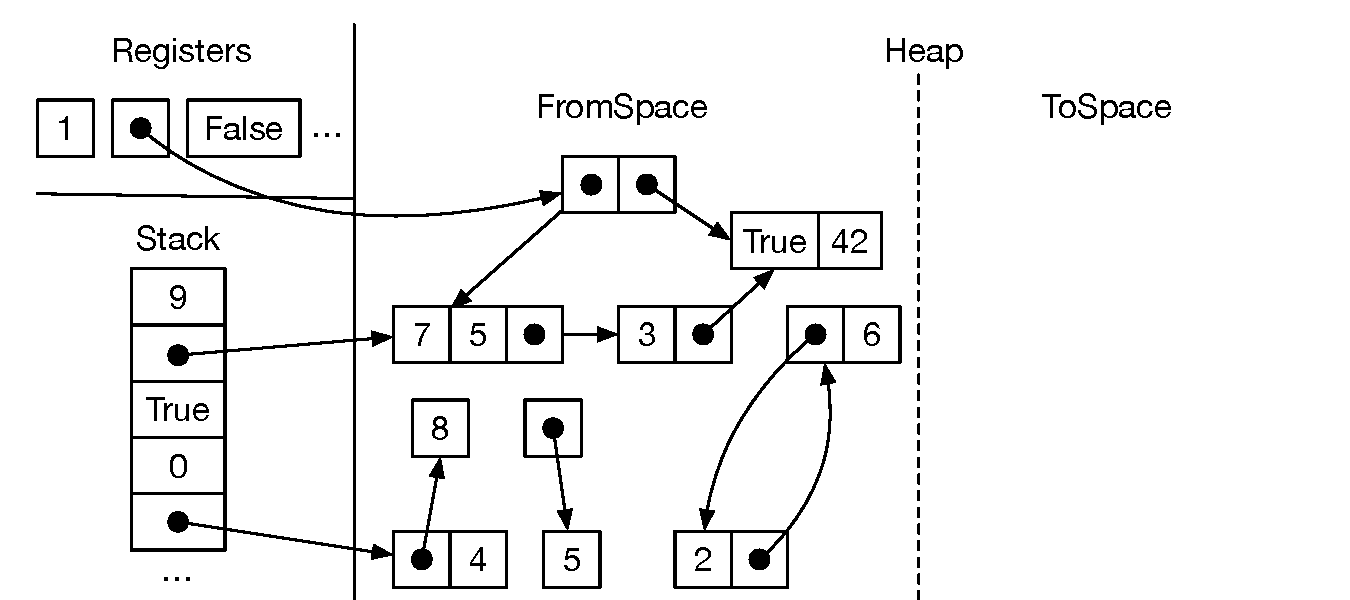
\includegraphics[width=\textwidth]{figs/copy-collect-1-python}}
\\[5ex]
\racket{\includegraphics[width=\textwidth]{figs/copy-collect-2}}
\python{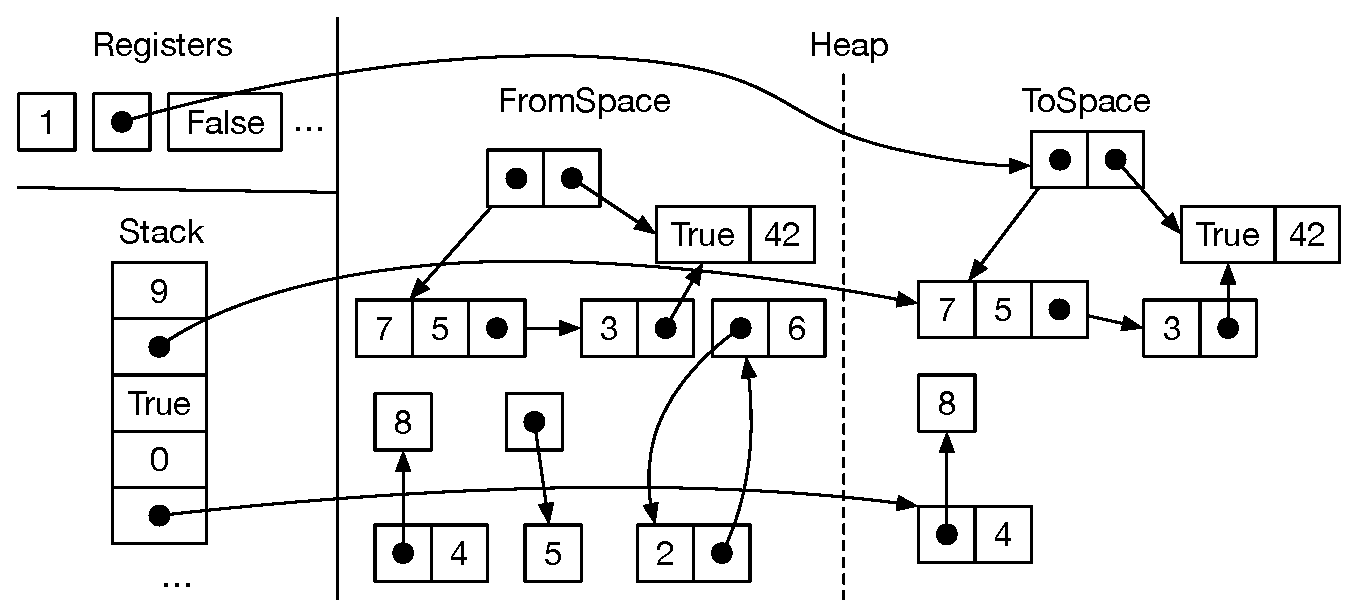
\includegraphics[width=\textwidth]{figs/copy-collect-2-python}}
\caption{A copying collector in action.}
\label{fig:copying-collector}
\end{figure}

\subsection{Graph Copying via Cheney's Algorithm}
\label{sec:cheney}
\index{subject}{Cheney's algorithm}
Let us take a closer look at the copying of the live objects. The
allocated objects and pointers can be viewed as a graph and we need to
copy the part of the graph that is reachable from the root set. To
make sure we copy all of the reachable vertices in the graph, we need
an exhaustive graph traversal algorithm, such as depth-first search or
breadth-first search~\citep{Moore:1959aa,Cormen:2001uq}. Recall that
such algorithms take into account the possibility of cycles by marking
which vertices have already been visited, so as to ensure termination
of the algorithm. These search algorithms also use a data structure
such as a stack or queue as a to-do list to keep track of the vertices
that need to be visited. We use breadth-first search and a trick
due to \citet{Cheney:1970aa} for simultaneously representing the queue
and copying tuples into the ToSpace.

Figure~\ref{fig:cheney} shows several snapshots of the ToSpace as the
copy progresses. The queue is represented by a chunk of contiguous
memory at the beginning of the ToSpace, using two pointers to track
the front and the back of the queue, called the \emph{free pointer}
and the \emph{scan pointer} respectively. The algorithm starts by
copying all tuples that are immediately reachable from the root set
into the ToSpace to form the initial queue.  When we copy a tuple, we
mark the old tuple to indicate that it has been visited. We discuss
how this marking is accomplish in Section~\ref{sec:data-rep-gc}. Note
that any pointers inside the copied tuples in the queue still point
back to the FromSpace. Once the initial queue has been created, the
algorithm enters a loop in which it repeatedly processes the tuple at
the front of the queue and pops it off the queue.  To process a tuple,
the algorithm copies all the tuple that are directly reachable from it
to the ToSpace, placing them at the back of the queue. The algorithm
then updates the pointers in the popped tuple so they point to the
newly copied tuples.

\begin{figure}[tbp]
\centering
\racket{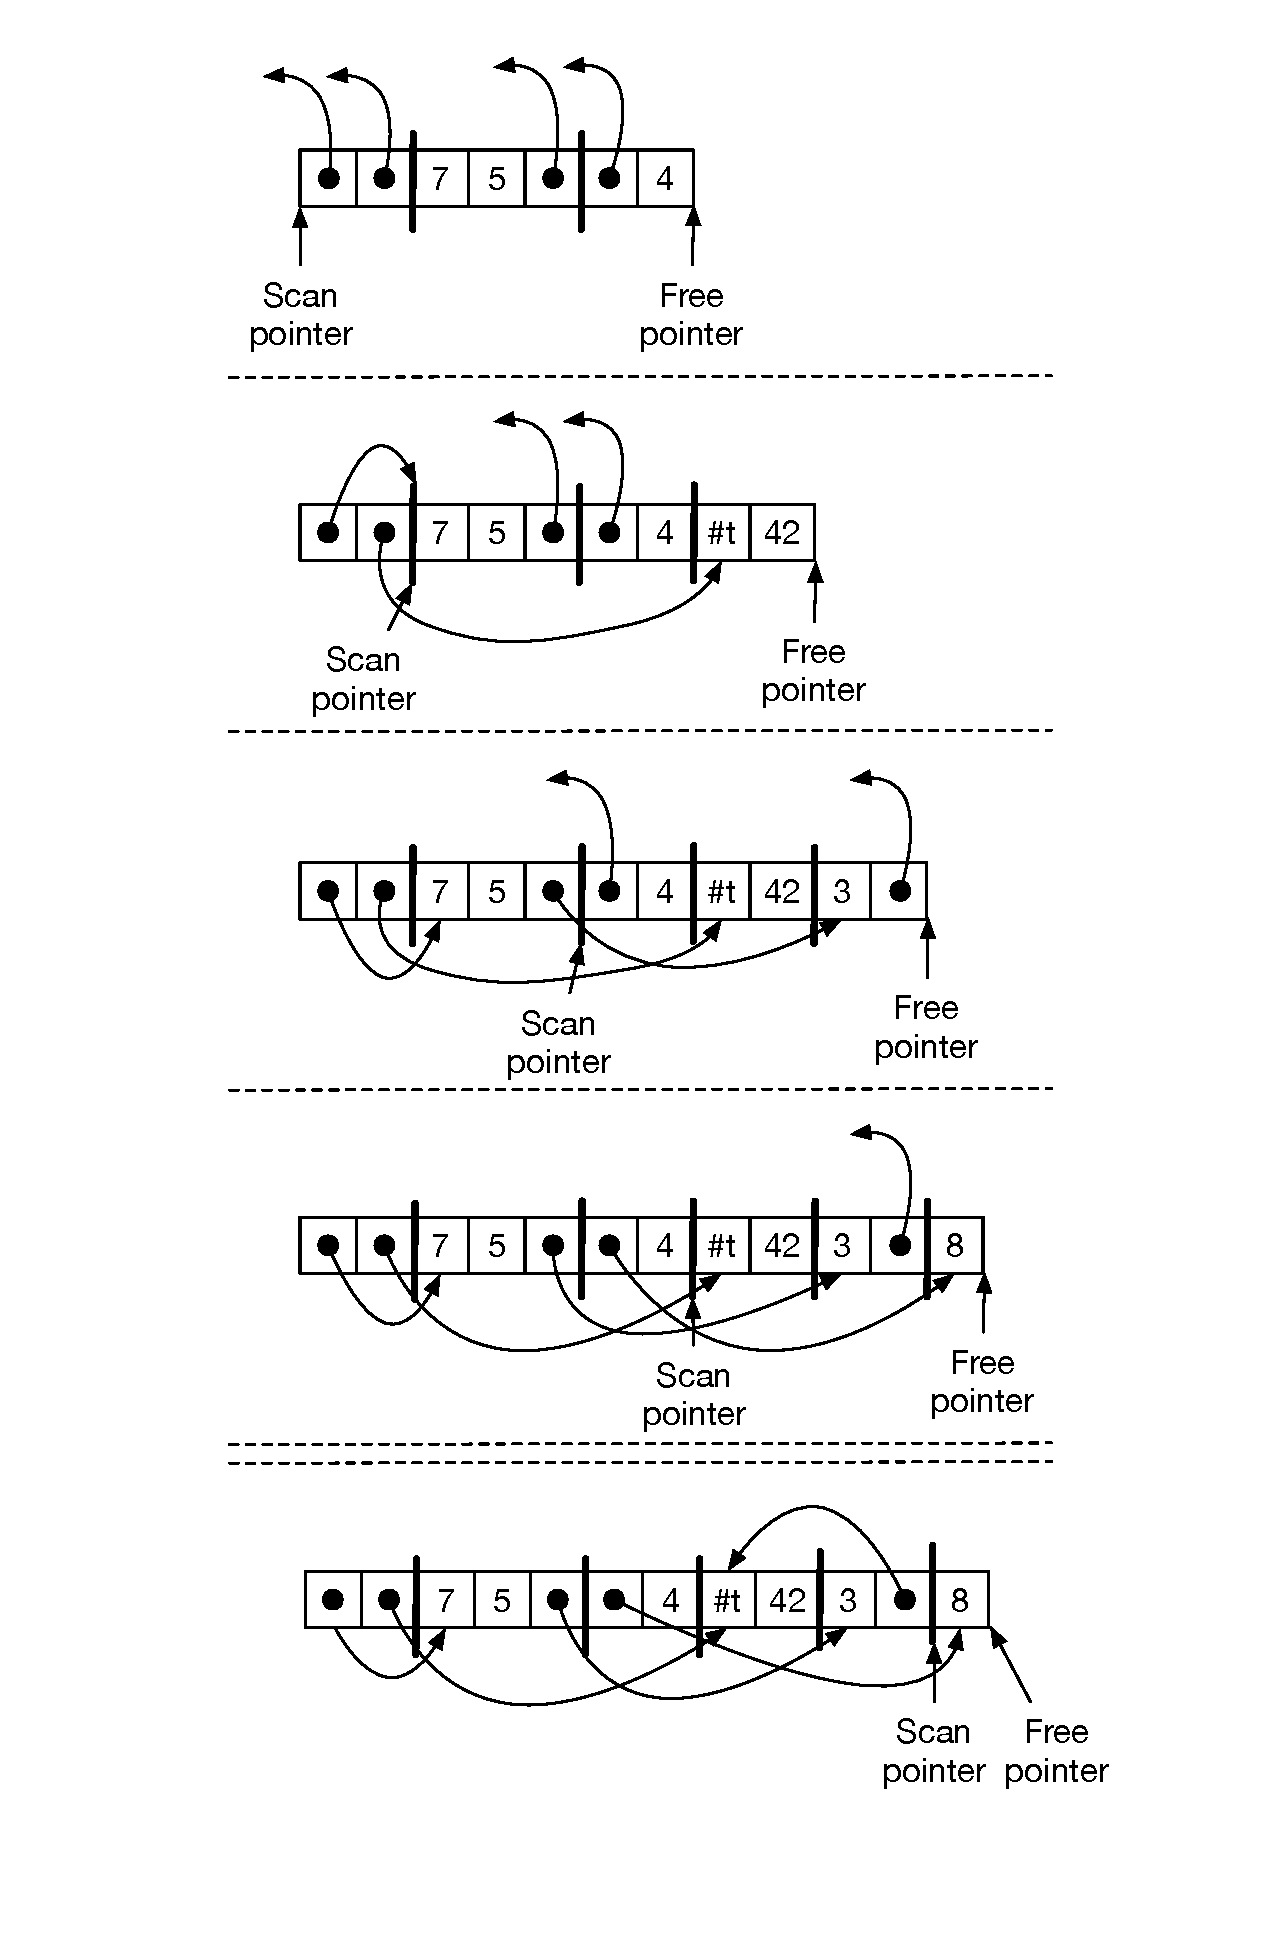
\includegraphics[width=0.9\textwidth]{figs/cheney}}
\python{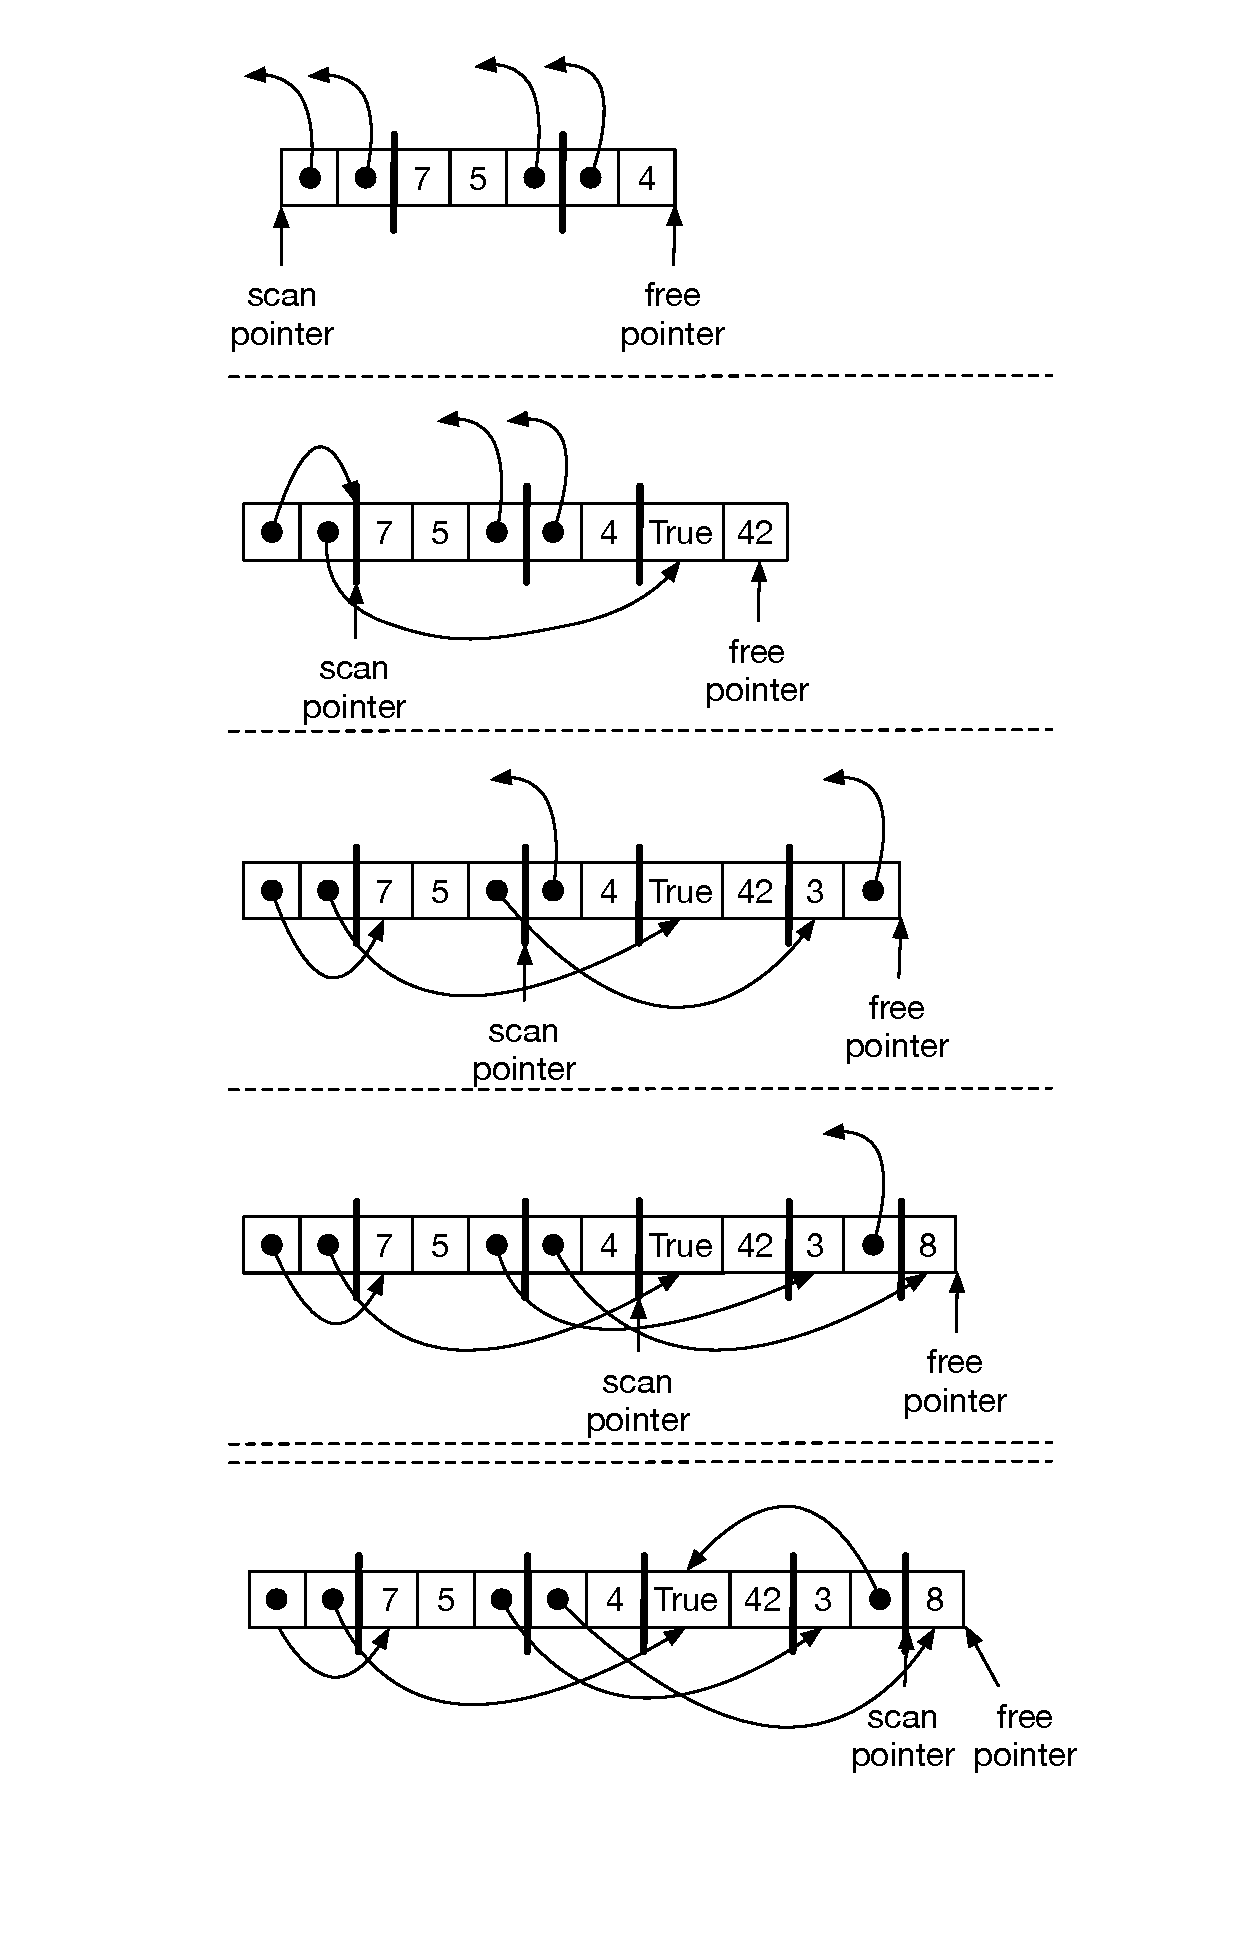
\includegraphics[width=0.9\textwidth]{figs/cheney-python}}
\caption{Depiction of the Cheney algorithm copying the live tuples.}
\label{fig:cheney}
\end{figure}

Getting back to Figure~\ref{fig:cheney}, in the first step we copy the
tuple whose second element is $42$ to the back of the queue. The other
pointer goes to a tuple that has already been copied, so we do not
need to copy it again, but we do need to update the pointer to the new
location. This can be accomplished by storing a \emph{forwarding
pointer}\index{subect}{forwarding pointer} to the new location in the
old tuple, back when we initially copied the tuple into the
ToSpace. This completes one step of the algorithm. The algorithm
continues in this way until the queue is empty, that is, when the scan
pointer catches up with the free pointer.


\subsection{Data Representation}
\label{sec:data-rep-gc}

The garbage collector places some requirements on the data
representations used by our compiler. First, the garbage collector
needs to distinguish between pointers and other kinds of data such as
integers. There are several ways to accomplish this.
\begin{enumerate}
\item Attached a tag to each object that identifies what type of
  object it is~\citep{McCarthy:1960dz}.
\item Store different types of objects in different
  regions~\citep{Steele:1977ab}.
\item Use type information from the program to either generate
  type-specific code for collecting or to generate tables that can
  guide the
  collector~\citep{Appel:1989aa,Goldberg:1991aa,Diwan:1992aa}.
\end{enumerate}
Dynamically typed languages, such as \racket{Racket}\python{Python},
need to tag objects anyways, so option 1 is a natural choice for those
languages.  However, \LangVec{} is a statically typed language, so it
would be unfortunate to require tags on every object, especially small
and pervasive objects like integers and Booleans.  Option 3 is the
best-performing choice for statically typed languages, but comes with
a relatively high implementation complexity. To keep this chapter
within a reasonable time budget, we recommend a combination of options
1 and 2, using separate strategies for the stack and the heap.

Regarding the stack, we recommend using a separate stack for pointers,
which we call the \emph{root stack}\index{subject}{root stack}
(a.k.a. ``shadow
stack'')~\citep{Siebert:2001aa,Henderson:2002aa,Baker:2009aa}. That
is, when a local variable needs to be spilled and is of type
\racket{\code{Vector}}\python{\code{TupleType}}, then we put it on the
root stack instead of putting it on the procedure call
stack. Furthermore, we always spill tuple-typed variables if they are
live during a call to the collector, thereby ensuring that no pointers
are in registers during a collection. Figure~\ref{fig:shadow-stack}
reproduces the example from Figure~\ref{fig:copying-collector} and
contrasts it with the data layout using a root stack. The root stack
contains the two pointers from the regular stack and also the pointer
in the second register.

\begin{figure}[tbp]
  \centering
  \racket{\includegraphics[width=0.60\textwidth]{figs/root-stack}}
  \python{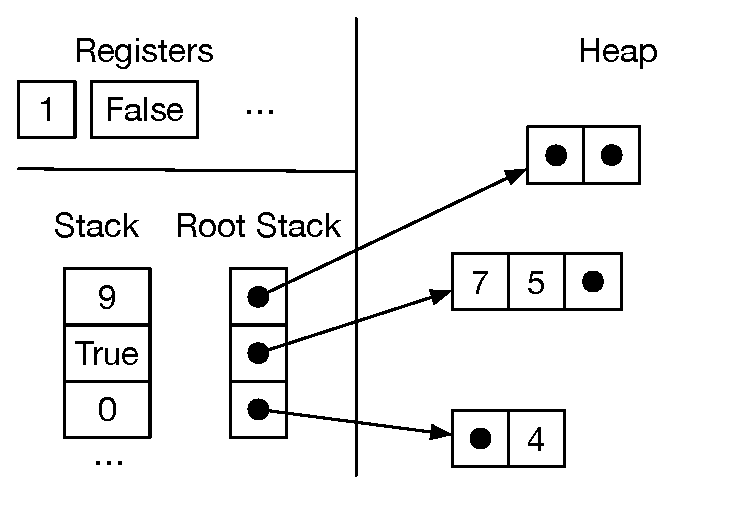
\includegraphics[width=0.60\textwidth]{figs/root-stack-python}}
\caption{Maintaining a root stack to facilitate garbage collection.}
\label{fig:shadow-stack}
\end{figure}

The problem of distinguishing between pointers and other kinds of data
also arises inside of each tuple on the heap. We solve this problem by
attaching a tag, an extra 64-bits, to each
tuple. Figure~\ref{fig:tuple-rep} zooms in on the tags for two of the
tuples in the example from Figure~\ref{fig:copying-collector}. Note
that we have drawn the bits in a big-endian way, from right-to-left,
with bit location 0 (the least significant bit) on the far right,
which corresponds to the direction of the x86 shifting instructions
\key{salq} (shift left) and \key{sarq} (shift right). Part of each tag
is dedicated to specifying which elements of the tuple are pointers,
the part labeled ``pointer mask''. Within the pointer mask, a 1 bit
indicates there is a pointer and a 0 bit indicates some other kind of
data. The pointer mask starts at bit location 7. We limit tuples to a
maximum size of 50 elements, so we just need 50 bits for the pointer
mask.%
%
\footnote{A production-quality compiler would handle
arbitrary-sized tuples and use a more complex approach.}
%
The tag also contains two other pieces of information. The length of
the tuple (number of elements) is stored in bits location 1 through
6. Finally, the bit at location 0 indicates whether the tuple has yet
to be copied to the ToSpace.  If the bit has value 1, then this tuple
has not yet been copied.  If the bit has value 0 then the entire tag
is a forwarding pointer. (The lower 3 bits of a pointer are always
zero anyways because our tuples are 8-byte aligned.)

\begin{figure}[tbp]
\centering 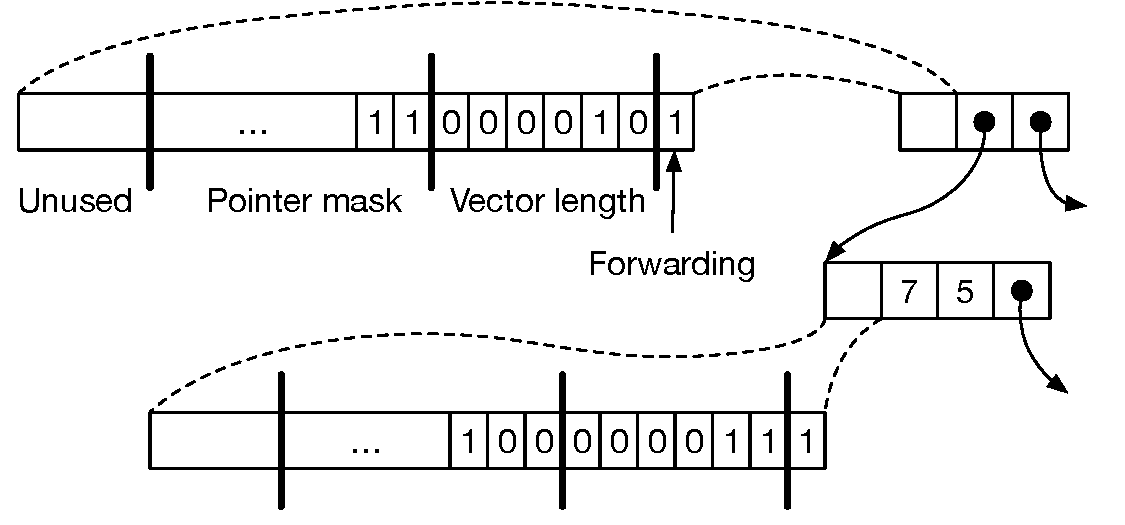
\includegraphics[width=0.8\textwidth]{figs/tuple-rep}
\caption{Representation of tuples in the heap.}
\label{fig:tuple-rep}
\end{figure}

\subsection{Implementation of the Garbage Collector}
\label{sec:organize-gz}
\index{subject}{prelude}

An implementation of the copying collector is provided in the
\code{runtime.c} file. Figure~\ref{fig:gc-header} defines the
interface to the garbage collector that is used by the compiler. The
\code{initialize} function creates the FromSpace, ToSpace, and root
stack and should be called in the prelude of the \code{main}
function. The arguments of \code{initialize} are the root stack size
and the heap size. Both need to be multiples of $64$ and $16384$ is a
good choice for both.  The \code{initialize} function puts the address
of the beginning of the FromSpace into the global variable
\code{free\_ptr}. The global variable \code{fromspace\_end} points to
the address that is 1-past the last element of the FromSpace. (We use
half-open intervals to represent chunks of
memory~\citep{Dijkstra:1982aa}.)  The \code{rootstack\_begin} variable
points to the first element of the root stack.

As long as there is room left in the FromSpace, your generated code
can allocate tuples simply by moving the \code{free\_ptr} forward.
%
The amount of room left in FromSpace is the difference between the
\code{fromspace\_end} and the \code{free\_ptr}.  The \code{collect}
function should be called when there is not enough room left in the
FromSpace for the next allocation.  The \code{collect} function takes
a pointer to the current top of the root stack (one past the last item
that was pushed) and the number of bytes that need to be
allocated. The \code{collect} function performs the copying collection
and leaves the heap in a state such that the next allocation will
succeed.

\begin{figure}[tbp]
\begin{lstlisting}
   void initialize(uint64_t rootstack_size, uint64_t heap_size);
   void collect(int64_t** rootstack_ptr, uint64_t bytes_requested);
   int64_t* free_ptr;
   int64_t* fromspace_begin;
   int64_t* fromspace_end;
   int64_t** rootstack_begin;
\end{lstlisting}
\caption{The compiler's interface to the garbage collector.}
\label{fig:gc-header}
\end{figure}

%% \begin{exercise}
%%   In the file \code{runtime.c} you will find the implementation of
%%   \code{initialize} and a partial implementation of \code{collect}.
%%   The \code{collect} function calls another function, \code{cheney},
%%   to perform the actual copy, and that function is left to the reader
%%   to implement. The following is the prototype for \code{cheney}.
%% \begin{lstlisting}
%%    static void cheney(int64_t** rootstack_ptr);
%% \end{lstlisting}
%%   The parameter \code{rootstack\_ptr} is a pointer to the top of the
%%   rootstack (which is an array of pointers).  The \code{cheney} function
%%   also communicates with \code{collect} through the global
%%   variables \code{fromspace\_begin} and \code{fromspace\_end}
%%   mentioned in Figure~\ref{fig:gc-header} as well as the pointers for
%%   the ToSpace:
%% \begin{lstlisting}
%%    static int64_t* tospace_begin;
%%    static int64_t* tospace_end;
%% \end{lstlisting}
%%   The job of the \code{cheney} function is to copy all the live
%%   objects (reachable from the root stack) into the ToSpace, update
%%   \code{free\_ptr} to point to the next unused spot in the ToSpace,
%%   update the root stack so that it points to the objects in the
%%   ToSpace, and finally to swap the global pointers for the FromSpace
%%   and ToSpace.
%% \end{exercise}

The introduction of garbage collection has a non-trivial impact on our
compiler passes. We introduce a new compiler pass named
\code{expose\_allocation}. We make significant changes to
\code{select\_instructions}, \code{build\_interference},
\code{allocate\_registers}, and \code{prelude\_and\_conclusion} and
make minor changes in several more passes.  The following program will
serve as our running example.  It creates two tuples, one nested
inside the other. Both tuples have length one. The program accesses
the element in the inner tuple.
% tests/vectors_test_17.rkt
{\if\edition\racketEd
\begin{lstlisting}
(vector-ref (vector-ref (vector (vector 42)) 0) 0)
\end{lstlisting}
\fi}
{\if\edition\pythonEd
\begin{lstlisting}
print( ((42,),)[0][0] )
\end{lstlisting}
\fi}


{\if\edition\racketEd
\section{Shrink}
\label{sec:shrink-Lvec}

Recall that the \code{shrink} pass translates the primitives operators
into a smaller set of primitives.
%
This pass comes after type checking and the type checker adds a
\code{HasType} AST node around each \code{vector} AST node, so you'll
need to add a case for \code{HasType} to the \code{shrink} pass.

\fi}

\section{Expose Allocation}
\label{sec:expose-allocation}

The pass \code{expose\_allocation} lowers tuple creation into a
conditional call to the collector followed by allocating the
appropriate amount of memory and initializing it.  We choose to place
the \code{expose\_allocation} pass before
\code{remove\_complex\_operands} because the code generated by
\code{expose\_allocation} contains complex operands.

The output of \code{expose\_allocation} is a language \LangAlloc{}
that extends \LangVec{} with new forms that we use in the translation
of tuple creation.
%
{\if\edition\racketEd
\[
\begin{array}{lcl}
  \Exp &::=& \cdots
      \MID (\key{collect} \,\itm{int})
      \MID (\key{allocate} \,\itm{int}\,\itm{type})
      \MID (\key{global-value} \,\itm{name}) 
\end{array}
\]
\fi}
{\if\edition\pythonEd
\[
\begin{array}{lcl}
  \Exp &::=& \cdots\\
      &\MID& \key{collect}(\itm{int})
      \MID \key{allocate}(\itm{int},\itm{type})
      \MID \key{global\_value}(\itm{name}) \\
      &\MID& \key{begin:} ~ \Stmt^{*} ~ \Exp \\
   \Stmt &::= & \CASSIGN{\CPUT{\Exp}{\itm{int}}}{\Exp}
\end{array}
\]

\fi}

The \CCOLLECT{$n$} form runs the garbage collector, requesting that it
make sure that there are $n$ bytes ready to be allocated. During
instruction selection, the \CCOLLECT{$n$} form will become a call to
the \code{collect} function in \code{runtime.c}.
%
The \CALLOCATE{$n$}{$T$} form obtains memory for $n$ elements (and
space at the front for the 64 bit tag), but the elements are not
initialized.  \index{subject}{allocate} The $T$ parameter is the type
of the tuple:
%
\VECTY{\racket{$\Type_1 \ldots \Type_n$}\python{$\Type_1, \ldots, \Type_n$}}
%
where $\Type_i$ is the type of the $i$th element in the tuple. The
\CGLOBALVALUE{\itm{name}} form reads the value of a global variable, such
as \code{free\_ptr}.
%
\python{The \code{begin} form is an expression that executes a
  sequence of statements and then produces the value of the expression
  at the end.}

The following shows the transformation of tuple creation into 1) a
sequence of temporary variables bindings for the initializing
expressions, 2) a conditional call to \code{collect}, 3) a call to
\code{allocate}, and 4) the initialization of the tuple. The
\itm{len} placeholder refers to the length of the tuple and
\itm{bytes} is how many total bytes need to be allocated for the
tuple, which is 8 for the tag plus \itm{len} times 8.
%
\python{The \itm{type} needed for the second argument of the
  \code{allocate} form can be obtained from the \code{has\_type} field
  of the tuple AST node, which is stored there by running the type
  checker for \LangVec{} immediately before this pass.}
%
\begin{center}
\begin{minipage}{\textwidth}
{\if\edition\racketEd
\begin{lstlisting}
  (has-type (vector |$e_0 \ldots e_{n-1}$|) |\itm{type}|)
|$\Longrightarrow$|
  (let ([|$x_0$| |$e_0$|]) ... (let ([|$x_{n-1}$| |$e_{n-1}$|])
  (let ([_ (if (< (+ (global-value free_ptr) |\itm{bytes}|)
                  (global-value fromspace_end))
               (void)
               (collect |\itm{bytes}|))])
  (let ([|$v$| (allocate |\itm{len}| |\itm{type}|)])
  (let ([_ (vector-set! |$v$| |$0$| |$x_0$|)]) ...
  (let ([_ (vector-set! |$v$| |$n-1$| |$x_{n-1}$|)])
     |$v$|) ... )))) ...)
\end{lstlisting}
\fi}
{\if\edition\pythonEd
\begin{lstlisting}
  (|$e_0$|, |$\ldots$|, |$e_{n-1}$|)
|$\Longrightarrow$|
  begin:
      |$x_0$| = |$e_0$|
           |$\vdots$|
      |$x_{n-1}$| = |$e_{n-1}$|
      if global_value(free_ptr) + |\itm{bytes}| < global_value(fromspace_end):
          0
      else:
          collect(|\itm{bytes}|)
      |$v$| = allocate(|\itm{len}|, |\itm{type}|)
      |$v$|[0] = |$x_0$|
           |$\vdots$|
      |$v$|[|$n-1$|] = |$x_{n-1}$|
      |$v$|
\end{lstlisting}
\fi}
\end{minipage}
\end{center}
%
\noindent The sequencing of the initializing expressions
$e_0,\ldots,e_{n-1}$ prior to the \code{allocate} is important, as
they may trigger garbage collection and we cannot have an allocated
but uninitialized tuple on the heap during a collection.

Figure~\ref{fig:expose-alloc-output} shows the output of the
\code{expose\_allocation} pass on our running example.

\begin{figure}[tbp]
  % tests/s2_17.rkt
{\if\edition\racketEd
\begin{lstlisting}
(vector-ref
 (vector-ref
  (let ([vecinit7976
         (let ([vecinit7972 42])
           (let ([collectret7974
                  (if (< (+ (global-value free_ptr) 16) 
                         (global-value fromspace_end))
                      (void)
                      (collect 16)
                      )])
             (let ([alloc7971 (allocate 1 (Vector Integer))])
               (let ([initret7973 (vector-set! alloc7971 0 vecinit7972)])
                 alloc7971))))])
    (let ([collectret7978
           (if (< (+ (global-value free_ptr) 16)
                  (global-value fromspace_end))
               (void)
               (collect 16)
               )])
      (let ([alloc7975 (allocate 1 (Vector (Vector Integer)))])
        (let ([initret7977 (vector-set! alloc7975 0 vecinit7976)])
          alloc7975))))
  0)
 0)
\end{lstlisting}
\fi}
{\if\edition\pythonEd
\begin{lstlisting}
print( |$T_1$|[0][0] )
\end{lstlisting}
where $T_1$ is
\begin{lstlisting}
    begin:
          tmp.1 = |$T_2$|
          if global_value(free_ptr) + 16 < global_value(fromspace_end):
              0
          else:
              collect(16)
          tmp.2 = allocate(1, TupleType(TupleType([int])))
          tmp.2[0] = tmp.1
          tmp.2
\end{lstlisting}
and $T_2$ is
\begin{lstlisting}
    begin:
          tmp.3 = 42
          if global_value(free_ptr) + 16 < global_value(fromspace_end):
              0
          else:
              collect(16)
          tmp.4 = allocate(1, TupleType([int]))
          tmp.4[0] = tmp.3
          tmp.4
\end{lstlisting}
\fi}
\caption{Output of the \code{expose\_allocation} pass.}
\label{fig:expose-alloc-output}
\end{figure}


\section{Remove Complex Operands}
\label{sec:remove-complex-opera-Lvec}

{\if\edition\racketEd
%
The forms \code{collect}, \code{allocate}, and \code{global\_value}
should be treated as complex operands.
%
\fi}
%
{\if\edition\pythonEd
%
The expressions \code{allocate}, \code{global\_value}, \code{begin},
and tuple access should be treated as complex operands.  The
sub-expressions of tuple access must be atomic.
%
\fi}
%% A new case for
%% \code{HasType} is needed and the case for \code{Prim} needs to be
%% handled carefully to prevent the \code{Prim} node from being separated
%% from its enclosing \code{HasType}.
Figure~\ref{fig:Lvec-anf-syntax}
shows the grammar for the output language \LangAllocANF{} of this
pass, which is \LangAlloc{} in monadic normal form.

\newcommand{\LtupMonadASTPython}{
\begin{array}{rcl}
\Exp &::=& \GET{\Atm}{\Atm} \\
     &\MID& \LEN{\Atm}\\
   &\MID& \ALLOCATE{\Int}{\Type}
    \MID \GLOBALVALUE{\Var} \\
\Stmt{} &::=& \ASSIGN{\PUT{\Atm}{\Atm}}{\Atm} \\
   &\MID& \COLLECT{\Int}
\end{array}
}

\begin{figure}[tp]
\centering
\fbox{
\begin{minipage}{0.96\textwidth}
\small
{\if\edition\racketEd    
\[
\begin{array}{rcl}
  \Atm &::=& \gray{ \INT{\Int} \MID \VAR{\Var} \MID \BOOL{\itm{bool}} 
       \MID \VOID{} } \\
\Exp &::=& \gray{ \Atm \MID \READ{} } \\
   &\MID& \gray{ \NEG{\Atm} \MID \ADD{\Atm}{\Atm} } \\
   &\MID& \gray{ \LET{\Var}{\Exp}{\Exp} } \\
   &\MID& \gray{ \UNIOP{\key{'not}}{\Atm} } \\
   &\MID& \gray{ \BINOP{\itm{cmp}}{\Atm}{\Atm} \MID \IF{\Exp}{\Exp}{\Exp} }\\
   &\MID& \COLLECT{\Int} \RP \MID \ALLOCATE{\Int}{\Type}
   \MID \GLOBALVALUE{\Var}\\
%  &\MID& \LP\key{HasType}~\Exp~\Type\RP \\
\LangAllocANFM{}  &::=& \gray{ \PROGRAM{\code{'()}}{\Exp} }
\end{array}
\]
\fi}
{\if\edition\pythonEd
\[
\begin{array}{l}
  \gray{\LvarMonadASTPython} \\ \hline
  \gray{\LifMonadASTPython} \\ \hline
  \gray{\LwhileMonadASTPython} \\ \hline
  \LtupMonadASTPython   \\
  \begin{array}{rcl}
     \LangAllocANFM{} &::=& \PROGRAM{\code{'()}}{\Stmt^{*}}
  \end{array}
\end{array}
%% \begin{array}{lcl}
%% \itm{binaryop} &::=& \code{Add()} \MID \code{Sub()} \\
%% \itm{boolop} &::=& \code{And()} \MID \code{Or()} \\
%% \itm{cmp} &::= & \code{Eq()} \MID \code{NotEq()} \MID \code{Lt()} \MID \code{LtE()} \MID \code{Gt()} \MID \code{GtE()} \MID \code{Is()} \\
%% \itm{unaryop} &::=& \code{USub()} \MID \code{Not()} \\
%% \itm{bool} &::=& \code{True} \MID \code{False} \\
%% \Atm &::=& \INT{\Int} \MID \VAR{\Var} \MID \BOOL{\itm{bool}} \\
%% \Exp &::=& \Atm \MID \READ{} \MID \\
%%      &\MID& \BINOP{\Atm}{\itm{binaryop}}{\Atm}
%%      \MID \UNIOP{\itm{unaryop}}{\Atm}\\
%%      &\MID& \CMP{\Atm}{\itm{cmp}}{\Atm} \\
%% %     \MID \BOOLOP{\itm{boolop}}{\Exp}{\Exp} \\ % removed by RCO
%%      &\MID& \IF{\Exp}{\Exp}{\Exp} \\
%%      &\MID& \GET{\Atm}{\Atm} \\
%%      &\MID& \LEN{\Exp}\\
%%    &\MID& \ALLOCATE{\Int}{\Type}
%%      \MID \GLOBALVALUE{\Var}\RP\\
%%    &\MID& \BEGIN{\Stmt^{*}}{\Atm} \\ % can use this in place of \LET;
%%                                 % why have \LET?
%% \Stmt{} &::=& \PRINT{\Atm} \MID \EXPR{\Exp} \\
%%   &\MID& \ASSIGN{\VAR{\Var}}{\Exp} \\
%%   &\MID& \ASSIGN{\PUT{\Atm}{\Atm}}{\Exp} \\
%%   &\MID& \IFSTMT{\Exp}{\Stmt^{+}}{\Stmt^{+}}\\
%%   &\MID& \WHILESTMT{\Exp}{\Stmt^{+}}
%%    \MID \COLLECT{\Int}  \\
%% \LangAllocANFM{} &::=& \PROGRAM{\code{'()}}{\Stmt^{*}}
%% \end{array}
\]
\fi}
\end{minipage}
}
\caption{\LangAllocANF{} is \LangAlloc{} in monadic normal form.}
\label{fig:Lvec-anf-syntax}
\end{figure}


\section{Explicate Control and the \LangCVec{} language}
\label{sec:explicate-control-r3}


\newcommand{\CtupASTRacket}{
\begin{array}{lcl}
\Exp &::= & \LP\key{Allocate} \,\itm{int}\,\itm{type}\RP \\
   &\MID& \VECREF{\Atm}{\INT{\Int}}  \\
   &\MID& \VECSET{\Atm}{\INT{\Int}}{\Atm} \\
   &\MID& \VECLEN{\Atm} \\
   &\MID& \GLOBALVALUE{\Var} \\
\Stmt &::=& \VECSET{\Atm}{\INT{\Int}}{\Atm} \\
    &\MID& \LP\key{Collect} \,\itm{int}\RP 
\end{array}
}
  
\newcommand{\CtupASTPython}{
\begin{array}{lcl}
\Exp &::= & \GET{\Atm}{\Atm} \MID \ALLOCATE{\Int}{\Type} \\
      &\MID& \GLOBALVALUE{\Var} \MID \LEN{\Atm} \\
\Stmt &::=& \COLLECT{\Int} \\
     &\MID& \ASSIGN{\PUT{\Atm}{\Atm}}{\Atm} 
\end{array}
}

\begin{figure}[tp]
\fbox{
  \begin{minipage}{0.96\textwidth}
    \small
{\if\edition\racketEd    
\[
\begin{array}{l}
  \gray{\CvarASTRacket} \\ \hline
  \gray{\CifASTRacket} \\ \hline
  \gray{\CloopASTRacket} \\ \hline
  \CtupASTRacket \\
  \begin{array}{lcl}
    \LangCVecM{} & ::= & \CPROGRAM{\itm{info}}{\LP\LP\itm{label}\,\key{.}\,\Tail\RP\ldots\RP}
  \end{array}
\end{array}
\]
\fi}
{\if\edition\pythonEd
\[
\begin{array}{l}
  \gray{\CifASTPython} \\ \hline
  \CtupASTPython \\
\begin{array}{lcl}
\LangCVecM{} & ::= & \CPROGRAM{\itm{info}}{\LC\itm{label}\key{:}\,\Stmt^{*}, \ldots \RC}
\end{array}
\end{array}
\]
\fi}
\end{minipage}
}
\caption{The abstract syntax of \LangCVec{}, extending
  \racket{\LangCLoop{} (Figure~\ref{fig:c7-syntax})}\python{\LangCIf{}
  (Figure~\ref{fig:c1-syntax})}.}
\label{fig:c2-syntax}
\end{figure}

The output of \code{explicate\_control} is a program in the
intermediate language \LangCVec{}, whose abstract syntax is defined in
Figure~\ref{fig:c2-syntax}.
%
\racket{(The concrete syntax is defined in
  Figure~\ref{fig:c2-concrete-syntax} of the Appendix.)}
%
The new expressions of \LangCVec{} include \key{allocate},
%
\racket{\key{vector-ref}, and \key{vector-set!},}
%
\python{accessing tuple elements,}
%
and \key{global\_value}.
%
\python{\LangCVec{} also includes the \code{collect} statement and
assignment to a tuple element.}
%
\racket{\LangCVec{} also includes the new \code{collect} statement.}
%
The \code{explicate\_control} pass can treat these new forms much like
the other forms that we've already encoutered.


\section{Select Instructions and the \LangXGlobal{} Language}
\label{sec:select-instructions-gc}
\index{subject}{instruction selection}

%% void (rep as zero)
%% allocate
%% collect (callq collect)
%% vector-ref
%% vector-set!
%% vector-length
%% global (postpone)

In this pass we generate x86 code for most of the new operations that
were needed to compile tuples, including \code{Allocate},
\code{Collect}, and accessing tuple elements.
%
We compile \code{GlobalValue} to \code{Global} because the later has a
different concrete syntax (see Figures~\ref{fig:x86-2-concrete} and
\ref{fig:x86-2}).  \index{subject}{x86}

The tuple read and write forms translate into \code{movq}
instructions.  (The plus one in the offset is to get past the tag at
the beginning of the tuple representation.)
%
\begin{center}
\begin{minipage}{\textwidth}
{\if\edition\racketEd    
\begin{lstlisting}
|$\itm{lhs}$| = (vector-ref |$\itm{tup}$| |$n$|);
|$\Longrightarrow$|
movq |$\itm{tup}'$|, %r11
movq |$8(n+1)$|(%r11), |$\itm{lhs'}$|

|$\itm{lhs}$| = (vector-set! |$\itm{tup}$| |$n$| |$\itm{rhs}$|);
|$\Longrightarrow$|
movq |$\itm{tup}'$|, %r11
movq |$\itm{rhs}'$|, |$8(n+1)$|(%r11)
movq $0, |$\itm{lhs'}$|
\end{lstlisting}
\fi}
{\if\edition\pythonEd    
\begin{lstlisting}
|$\itm{lhs}$| = |$\itm{tup}$|[|$n$|]
|$\Longrightarrow$|
movq |$\itm{tup}'$|, %r11
movq |$8(n+1)$|(%r11), |$\itm{lhs'}$|

|$\itm{tup}$|[|$n$|] = |$\itm{rhs}$|
|$\Longrightarrow$|
movq |$\itm{tup}'$|, %r11
movq |$\itm{rhs}'$|, |$8(n+1)$|(%r11)
\end{lstlisting}
\fi}
\end{minipage}
\end{center}
\racket{The $\itm{lhs}'$, $\itm{tup}'$, and $\itm{rhs}'$}
\python{The $\itm{tup}'$ and $\itm{rhs}'$}
are obtained by translating from \LangCVec{} to x86.
%
The move of $\itm{tup}'$ to
register \code{r11} ensures that offset expression
\code{$-8(n+1)$(\%r11)} contains a register operand.  This requires
removing \code{r11} from consideration by the register allocating.

Why not use \code{rax} instead of \code{r11}? Suppose we instead used
\code{rax}. Then the generated code for tuple assignment would be
\begin{lstlisting}
movq |$\itm{tup}'$|, %rax
movq |$\itm{rhs}'$|, |$8(n+1)$|(%rax)
\end{lstlisting}
Next, suppose that $\itm{rhs}'$ ends up as a stack location, so
\code{patch\_instructions} would insert a move through \code{rax}
as follows.
\begin{lstlisting}
movq |$\itm{tup}'$|, %rax
movq |$\itm{rhs}'$|, %rax
movq %rax, |$8(n+1)$|(%rax)
\end{lstlisting}
But the above sequence of instructions does not work because we're
trying to use \code{rax} for two different values ($\itm{tup}'$ and
$\itm{rhs}'$) at the same time!

The \racket{\code{vector-length}}\python{\code{len}} operation should
be translated into a sequence of instructions that read the tag of the
tuple and extract the six bits that represent the tuple length, which
are the bits starting at index 1 and going up to and including bit 6.
The x86 instructions \code{andq} (for bitwise-and) and \code{sarq}
(shift right) can be used to accomplish this.

We compile the \code{allocate} form to operations on the
\code{free\_ptr}, as shown below. This approach is called \emph{inline
  allocation} as it implements allocation without a function call, by
simply bumping the allocation pointer. It is much more efficient than
calling a function for each allocation. The address in the
\code{free\_ptr} is the next free address in the FromSpace, so we copy
it into \code{r11} and then move it forward by enough space for the
tuple being allocated, which is $8(\itm{len}+1)$ bytes because each
element is 8 bytes (64 bits) and we use 8 bytes for the tag.  We then
initialize the \itm{tag} and finally copy the address in \code{r11} to
the left-hand-side. Refer to Figure~\ref{fig:tuple-rep} to see how the
tag is organized.
%
\racket{We recommend using the Racket operations
\code{bitwise-ior} and \code{arithmetic-shift} to compute the tag
during compilation.}
%
\python{We recommend using the bitwise-or operator \code{|} and the
  shift-left operator \code{<<} to compute the tag during
  compilation.}
%
The type annotation in the \code{allocate} form is used to determine
the pointer mask region of the tag.
%
The addressing mode \verb!free_ptr(%rip)! essentially stands for the
address of the \code{free\_ptr} global variable but uses a special
instruction-pointer relative addressing mode of the x86-64 processor.
In particular, the assembler computes the distance $d$ between the
address of \code{free\_ptr} and where the \code{rip} would be at that
moment and then changes the \code{free\_ptr(\%rip)} argument to
\code{$d$(\%rip)}, which at runtime will compute the address of
\code{free\_ptr}.
%
{\if\edition\racketEd
\begin{lstlisting}
   |$\itm{lhs}$| = (allocate |$\itm{len}$| (Vector |$\itm{type} \ldots$|));
   |$\Longrightarrow$|
   movq free_ptr(%rip), %r11
   addq |$8(\itm{len}+1)$|, free_ptr(%rip)
   movq $|$\itm{tag}$|, 0(%r11)
   movq %r11, |$\itm{lhs}'$|
\end{lstlisting}
\fi}
{\if\edition\pythonEd    
\begin{lstlisting}
   |$\itm{lhs}$| = allocate(|$\itm{len}$|, TupleType([|$\itm{type}, \ldots$])|);
   |$\Longrightarrow$|
   movq free_ptr(%rip), %r11
   addq |$8(\itm{len}+1)$|, free_ptr(%rip)
   movq $|$\itm{tag}$|, 0(%r11)
   movq %r11, |$\itm{lhs}'$|
\end{lstlisting}
\fi}
The \code{collect} form is compiled to a call to the \code{collect}
function in the runtime. The arguments to \code{collect} are 1) the
top of the root stack and 2) the number of bytes that need to be
allocated.  We use another dedicated register, \code{r15}, to
store the pointer to the top of the root stack. So \code{r15} is not
available for use by the register allocator.
{\if\edition\racketEd
\begin{lstlisting}
   (collect |$\itm{bytes}$|)
   |$\Longrightarrow$|
   movq %r15, %rdi
   movq $|\itm{bytes}|, %rsi
   callq collect
\end{lstlisting}
\fi}
{\if\edition\pythonEd    
\begin{lstlisting}
   collect(|$\itm{bytes}$|)
   |$\Longrightarrow$|
   movq %r15, %rdi
   movq $|\itm{bytes}|, %rsi
   callq collect
\end{lstlisting}
\fi}


\begin{figure}[tp]
\fbox{
\begin{minipage}{0.96\textwidth}
\[
\begin{array}{lcl}
  \Arg &::=& \gray{ \key{\$}\Int \MID \key{\%}\Reg \MID \Int\key{(}\key{\%}\Reg\key{)} \MID \key{\%}\itm{bytereg} } \MID \Var \key{(\%rip)} \\
\LangXGlobalM{} &::= & \gray{ \key{.globl main} }\\
      &    & \gray{ \key{main:} \; \Instr^{*} }
\end{array}
\]
\end{minipage}
}
\caption{The concrete syntax of \LangXGlobal{}  (extends \LangXIf{} of Figure~\ref{fig:x86-1-concrete}).}
\label{fig:x86-2-concrete}
\end{figure}

\begin{figure}[tp]
\fbox{
  \begin{minipage}{0.96\textwidth}
    \small
\[
\begin{array}{lcl}
  \Arg &::=&  \gray{  \INT{\Int} \MID \REG{\Reg} \MID \DEREF{\Reg}{\Int}
   \MID \BYTEREG{\Reg}} \\
   &\MID& \GLOBAL{\Var} \\
\LangXGlobalM{} &::= & \gray{ \XPROGRAM{\itm{info}}{\LP\LP\itm{label} \,\key{.}\, \Block \RP\ldots\RP} }
\end{array}
\]
\end{minipage}
}
\caption{The abstract syntax of \LangXGlobal{} (extends \LangXIf{} of Figure~\ref{fig:x86-1}).}
\label{fig:x86-2}
\end{figure}

The concrete and abstract syntax of the \LangXGlobal{} language is
defined in Figures~\ref{fig:x86-2-concrete} and \ref{fig:x86-2}.  It
differs from \LangXIf{} just in the addition of global variables.
%
Figure~\ref{fig:select-instr-output-gc} shows the output of the
\code{select\_instructions} pass on the running example.

\begin{figure}[tbp]
\centering
% tests/s2_17.rkt
\begin{minipage}[t]{0.5\textwidth}
\begin{lstlisting}[basicstyle=\ttfamily\scriptsize]
block35:
    movq free_ptr(%rip), alloc9024
    addq $16, free_ptr(%rip)
    movq alloc9024, %r11
    movq $131, 0(%r11)
    movq alloc9024, %r11
    movq vecinit9025, 8(%r11)
    movq $0, initret9026
    movq alloc9024, %r11
    movq 8(%r11), tmp9034
    movq tmp9034, %r11
    movq 8(%r11), %rax
    jmp conclusion
block36:
    movq $0, collectret9027
    jmp block35
block38:
    movq free_ptr(%rip), alloc9020
    addq $16, free_ptr(%rip)
    movq alloc9020, %r11
    movq $3, 0(%r11)
    movq alloc9020, %r11
    movq vecinit9021, 8(%r11)
    movq $0, initret9022
    movq alloc9020, vecinit9025
    movq free_ptr(%rip), tmp9031
    movq tmp9031, tmp9032
    addq $16, tmp9032
    movq fromspace_end(%rip), tmp9033
    cmpq tmp9033, tmp9032
    jl block36
    jmp block37
block37:
    movq %r15, %rdi
    movq $16, %rsi
    callq 'collect
    jmp block35
block39:
    movq $0, collectret9023
    jmp block38
\end{lstlisting}
\end{minipage}
\begin{minipage}[t]{0.45\textwidth}
\begin{lstlisting}[basicstyle=\ttfamily\scriptsize]
start:
    movq $42, vecinit9021
    movq free_ptr(%rip), tmp9028
    movq tmp9028, tmp9029
    addq $16, tmp9029
    movq fromspace_end(%rip), tmp9030
    cmpq tmp9030, tmp9029
    jl block39
    jmp block40
block40:
    movq %r15, %rdi
    movq $16, %rsi
    callq 'collect
    jmp block38
\end{lstlisting}
\end{minipage}
\caption{Output of the \code{select\_instructions} pass.}
\label{fig:select-instr-output-gc}
\end{figure}

\clearpage

\section{Register Allocation}
\label{sec:reg-alloc-gc}
\index{subject}{register allocation}

As discussed earlier in this chapter, the garbage collector needs to
access all the pointers in the root set, that is, all variables that
are tuples. It will be the responsibility of the register allocator
to make sure that:
\begin{enumerate}
\item the root stack is used for spilling tuple-typed variables, and
\item if a tuple-typed variable is live during a call to the
  collector, it must be spilled to ensure it is visible to the
  collector.
\end{enumerate}

The later responsibility can be handled during construction of the
interference graph, by adding interference edges between the call-live
tuple-typed variables and all the callee-saved registers. (They
already interfere with the caller-saved registers.)
%
\racket{The type information for variables is in the \code{Program}
  form, so we recommend adding another parameter to the
  \code{build\_interference} function to communicate this alist.}
%
\python{The type information for variables is generated by the type
  checker for \LangCVec{}, stored a field named \code{var\_types} in
  the \code{CProgram} AST mode. You'll need to propagate that
  information so that it is available in this pass.}

The spilling of tuple-typed variables to the root stack can be handled
after graph coloring, when choosing how to assign the colors
(integers) to registers and stack locations. The
\racket{\code{Program}}\python{\code{CProgram}} output of this pass
changes to also record the number of spills to the root stack.

% build-interference
%
% callq
%   extra parameter for var->type assoc. list
% update 'program' and 'if'

% allocate-registers
%    allocate spilled vectors to the rootstack

% don't change color-graph

% TODO:
%\section{Patch Instructions}
%[mention that global variables are memory references]

\section{Prelude and Conclusion}
\label{sec:print-x86-gc}
\label{sec:prelude-conclusion-x86-gc}
\index{subject}{prelude}\index{subject}{conclusion}

Figure~\ref{fig:print-x86-output-gc} shows the output of the
\code{prelude\_and\_conclusion} pass on the running example. In the
prelude and conclusion of the \code{main} function, we allocate space
on the root stack to make room for the spills of tuple-typed
variables. We do so by bumping the root stack
pointer (\code{r15}) taking care that the root stack grows up instead of down.  For the running
example, there was just one spill so we increment \code{r15} by 8
bytes. In the conclusion we decrement \code{r15} by 8 bytes. 

One issue that deserves special care is that there may be a call to
\code{collect} prior to the initializing assignments for all the
variables in the root stack. We do not want the garbage collector to
accidentally think that some uninitialized variable is a pointer that
needs to be followed. Thus, we zero-out all locations on the root
stack in the prelude of \code{main}. In
Figure~\ref{fig:print-x86-output-gc}, the instruction
%
\lstinline{movq $0, 0(%r15)}
%
is sufficient to accomplish this task because there is only one spill.
In general, we have to clear as many words as there are spills of
tuple-typed variables. The garbage collector tests each root to see
if it is null prior to dereferencing it. 

\begin{figure}[htbp]
  % TODO: Python Version -Jeremy
\begin{minipage}[t]{0.5\textwidth}
\begin{lstlisting}[basicstyle=\ttfamily\scriptsize]
block35:
	movq	free_ptr(%rip), %rcx
	addq	$16, free_ptr(%rip)
	movq	%rcx, %r11
	movq	$131, 0(%r11)
	movq	%rcx, %r11
	movq	-8(%r15), %rax
	movq	%rax, 8(%r11)
	movq	$0, %rdx
	movq	%rcx, %r11
	movq	8(%r11), %rcx
	movq	%rcx, %r11
	movq	8(%r11), %rax
	jmp conclusion
block36:
	movq	$0, %rcx
	jmp block35
block38:
	movq	free_ptr(%rip), %rcx
	addq	$16, free_ptr(%rip)
	movq	%rcx, %r11
	movq	$3, 0(%r11)
	movq	%rcx, %r11
	movq	%rbx, 8(%r11)
	movq	$0, %rdx
	movq	%rcx, -8(%r15)
	movq	free_ptr(%rip), %rcx
	addq	$16, %rcx
	movq	fromspace_end(%rip), %rdx
	cmpq	%rdx, %rcx
	jl block36
	movq	%r15, %rdi
	movq	$16, %rsi
	callq	collect
	jmp block35
block39:
	movq	$0, %rcx
	jmp block38
\end{lstlisting}
\end{minipage}
\begin{minipage}[t]{0.45\textwidth}
\begin{lstlisting}[basicstyle=\ttfamily\scriptsize]
start:
	movq	$42, %rbx
	movq	free_ptr(%rip), %rdx
	addq	$16, %rdx
	movq	fromspace_end(%rip), %rcx
	cmpq	%rcx, %rdx
	jl block39
	movq	%r15, %rdi
	movq	$16, %rsi
	callq	collect
	jmp block38
        
	.globl main
main:
	pushq	%rbp
	movq	%rsp, %rbp
	pushq	%r13
	pushq	%r12
	pushq	%rbx
	pushq	%r14
	subq	$0, %rsp
	movq $16384, %rdi
	movq $16384, %rsi
	callq initialize
	movq rootstack_begin(%rip), %r15
	movq $0, 0(%r15)
	addq $8, %r15
	jmp start
conclusion:
	subq $8, %r15
	addq	$0, %rsp
	popq	%r14
	popq	%rbx
	popq	%r12
	popq	%r13
	popq	%rbp
	retq
\end{lstlisting}
\end{minipage}
\caption{Output of the \code{prelude\_and\_conclusion} pass.}
\label{fig:print-x86-output-gc}
\end{figure}


\begin{figure}[tbp]
\begin{tikzpicture}[baseline=(current  bounding  box.center)]
\node (Lvec) at (0,2)  {\large \LangVec{}};
\node (Lvec-2) at (3,2)  {\large \LangVec{}};
\node (Lvec-3) at (6,2)  {\large \LangVec{}};
\node (Lvec-4) at (9,2)  {\large \LangVec{}};
\node (Lvec-5) at (9,0)  {\large \LangAllocANF{}};
\node (C2-4) at (3,0)  {\large \LangCVec{}};

\node (x86-2) at (3,-2)  {\large \LangXGlobalVar{}};
\node (x86-2-1) at (3,-4)  {\large \LangXGlobalVar{}};
\node (x86-2-2) at (6,-4)  {\large \LangXGlobalVar{}};
\node (x86-3) at (6,-2)  {\large \LangXGlobalVar{}};
\node (x86-4) at (9,-2) {\large \LangXGlobal{}};
\node (x86-5) at (9,-4) {\large \LangXGlobal{}};


%\path[->,bend left=15] (Lvec) edge [above] node {\ttfamily\footnotesize type-check} (Lvec-2);
\path[->,bend left=15] (Lvec) edge [above] node {\ttfamily\footnotesize shrink} (Lvec-2);
\path[->,bend left=15] (Lvec-2) edge [above] node {\ttfamily\footnotesize uniquify} (Lvec-3);
\path[->,bend left=15] (Lvec-3) edge [above] node {\ttfamily\footnotesize expose\_alloc.} (Lvec-4);
\path[->,bend left=15] (Lvec-4) edge [above] node {\ttfamily\footnotesize remove\_complex.} (Lvec-5);
\path[->,bend left=10] (Lvec-5) edge [above] node {\ttfamily\footnotesize explicate\_control} (C2-4);
\path[->,bend left=15] (C2-4) edge [right] node {\ttfamily\footnotesize select\_instr.} (x86-2);
\path[->,bend right=15] (x86-2) edge [left] node {\ttfamily\footnotesize uncover\_live} (x86-2-1);
\path[->,bend right=15] (x86-2-1) edge [below] node {\ttfamily\footnotesize build\_inter.} (x86-2-2);
\path[->,bend right=15] (x86-2-2) edge [right] node {\ttfamily\footnotesize allocate\_reg.} (x86-3);
\path[->,bend left=15] (x86-3) edge [above] node {\ttfamily\footnotesize patch\_instr.} (x86-4);
\path[->,bend left=15] (x86-4) edge [right] node {\ttfamily\footnotesize print\_x86} (x86-5);
\end{tikzpicture}
\caption{Diagram of the passes for \LangVec{}, a language with tuples.}
\label{fig:Lvec-passes}
\end{figure}

Figure~\ref{fig:Lvec-passes} gives an overview of all the passes needed
for the compilation of \LangVec{}.

\clearpage

{\if\edition\racketEd
\section{Challenge: Simple Structures}
\label{sec:simple-structures}
\index{subject}{struct}
\index{subject}{structure}

The language \LangStruct{} extends \LangVec{} with support for simple
structures. Its concrete syntax is defined in
Figure~\ref{fig:Lstruct-concrete-syntax} and the abstract syntax is in
Figure~\ref{fig:Lstruct-syntax}. Recall that a \code{struct} in Typed
Racket is a user-defined data type that contains named fields and that
is heap allocated, similar to a vector. The following is an example of
a structure definition, in this case the definition of a \code{point}
type.
\begin{lstlisting}
(struct point ([x : Integer] [y : Integer]) #:mutable)
\end{lstlisting}

\newcommand{\LstructGrammarRacket}{
\begin{array}{lcl}
  \Type &::=& \Var \\
  \Exp &::=& (\Var\;\Exp \ldots)\\
  \Def &::=& (\key{struct}\; \Var \; ([\Var \,\key{:}\, \Type] \ldots)\; \code{\#:mutable})\\
\end{array}
}
\newcommand{\LstructASTRacket}{
\begin{array}{lcl}
  \Type &::=& \VAR{\Var} \\
  \Exp &::=& \APPLY{\Var}{\Exp\ldots} \\
  \Def &::=& \LP\key{StructDef}\; \Var \; \LP\LS\Var \,\key{:}\, \Type\RS \ldots\RP\RP 
\end{array}
}

\begin{figure}[tbp]
\centering
\fbox{
\begin{minipage}{0.96\textwidth}
\[
\begin{array}{l}
  \gray{\LintGrammarRacket{}} \\ \hline
  \gray{\LvarGrammarRacket{}} \\ \hline
  \gray{\LifGrammarRacket{}} \\ \hline
  \gray{\LwhileGrammarRacket} \\ \hline
  \gray{\LtupGrammarRacket} \\  \hline
  \LstructGrammarRacket \\
\begin{array}{lcl}
  \LangStruct{} &::=& \Def \ldots \; \Exp
\end{array}
\end{array}
\]
\end{minipage}
}
\caption{The concrete syntax of \LangStruct{}, extending \LangVec{}
  (Figure~\ref{fig:Lvec-concrete-syntax}).}
\label{fig:Lstruct-concrete-syntax}
\end{figure}

\begin{figure}[tbp]
\centering
\fbox{
\begin{minipage}{0.96\textwidth}
\[
\begin{array}{l}
  \gray{\LintASTRacket{}} \\ \hline
  \gray{\LvarASTRacket{}} \\ \hline
  \gray{\LifASTRacket{}} \\ \hline
  \gray{\LwhileASTRacket} \\ \hline
  \gray{\LtupASTRacket} \\  \hline
  \LstructASTRacket \\
\begin{array}{lcl}
  \LangStruct{} &::=& \PROGRAMDEFSEXP{\code{'()}}{\LP\Def\ldots\RP)}{\Exp}
\end{array}
\end{array}
\]
\end{minipage}
}
\caption{The abstract syntax of \LangStruct{}, extending \LangVec{}
  (Figure~\ref{fig:Lvec-syntax}).}
\label{fig:Lstruct-syntax}
\end{figure}

An instance of a structure is created using function call syntax, with
the name of the structure in the function position:
\begin{lstlisting}
(point 7 12)
\end{lstlisting}
Function-call syntax is also used to read the value in a field of a
structure. The function name is formed by the structure name, a dash,
and the field name. The following example uses \code{point-x} and
\code{point-y} to access the \code{x} and \code{y} fields of two point
instances.
\begin{center}
\begin{lstlisting}
(let ([pt1 (point 7 12)])
  (let ([pt2 (point 4 3)])
    (+ (- (point-x pt1) (point-x pt2))
       (- (point-y pt1) (point-y pt2)))))
\end{lstlisting}
\end{center}
Similarly, to write to a field of a structure, use its set function,
whose name starts with \code{set-}, followed by the structure name,
then a dash, then the field name, and concluded with an exclamation
mark. The following example uses \code{set-point-x!} to change the
\code{x} field from \code{7} to \code{42}.
\begin{center}
  \begin{lstlisting}
(let ([pt (point 7 12)])
  (let ([_ (set-point-x! pt 42)])
    (point-x pt)))
\end{lstlisting}
\end{center}

\begin{exercise}\normalfont\normalsize
  Create a type checker for \LangStruct{} by extending the type
  checker for \LangVec{}. Extend your compiler with support for simple
  structures, compiling \LangStruct{} to x86 assembly code. Create
  five new test cases that use structures and test your compiler.
\end{exercise}

% TODO: create an interpreter for L_struct

\clearpage

\section{Challenge: Arrays}
\label{sec:arrays}

In Chapter~\ref{ch:Lvec} we studied tuples, that is, sequences of
elements whose length is determined at compile-time and where each
element of a tuple may have a different type (they are
heterogeous). This challenge is also about sequences, but this time
the length is determined at run-time and all the elements have the same
type (they are homogeneous). We use the term ``array'' for this later
kind of sequence.

The Racket language does not distinguish between tuples and arrays,
they are both represented by vectors. However, Typed Racket
distinguishes between tuples and arrays: the \code{Vector} type is for
tuples and the \code{Vectorof} type is for arrays.
%
Figure~\ref{fig:Lvecof-concrete-syntax} defines the concrete syntax
for \LangArray{}, extending \LangLoop{} with the \code{Vectorof} type
and the \code{make-vector} primitive operator for creating an array,
whose arguments are the length of the array and an initial value for
all the elements in the array. The \code{vector-length},
\code{vector-ref}, and \code{vector-ref!} operators that we defined
for tuples become overloaded for use with arrays.
%
We also include integer multiplication in \LangArray{}, as it is
useful in many examples involving arrays such as computing the
inner-product of two arrays (Figure~\ref{fig:inner-product}).


\begin{figure}[tp]
\centering
\fbox{
  \begin{minipage}{0.96\textwidth}
    \small
{\if\edition\racketEd    
\[
\begin{array}{lcl}
  \Type &::=& \ldots \MID \LP \key{Vectorof}~\Type \RP \\
  \Exp &::=& \gray{ \Int \MID \CREAD{} \MID \CNEG{\Exp}
     \MID \CADD{\Exp}{\Exp} \MID \CSUB{\Exp}{\Exp} }  \MID \CMUL{\Exp}{\Exp}\\
    &\MID&  \gray{ \Var \MID \CLET{\Var}{\Exp}{\Exp} }\\
    &\MID& \gray{\key{\#t} \MID \key{\#f} 
     \MID \LP\key{and}\;\Exp\;\Exp\RP 
     \MID \LP\key{or}\;\Exp\;\Exp\RP 
     \MID \LP\key{not}\;\Exp\RP } \\
    &\MID& \gray{ \LP\key{eq?}\;\Exp\;\Exp\RP \MID \CIF{\Exp}{\Exp}{\Exp} } \\
    &\MID& \gray{ \LP\key{vector}\;\Exp\ldots\RP \MID
          \LP\key{vector-ref}\;\Exp\;\Int\RP} \\
    &\MID& \gray{\LP\key{vector-set!}\;\Exp\;\Int\;\Exp\RP\MID \LP\key{void}\RP
    \MID \LP\Exp \; \Exp\ldots\RP } \\
    &\MID& \gray{ \LP \key{procedure-arity}~\Exp\RP 
    \MID \CLAMBDA{\LP\LS\Var \key{:} \Type\RS\ldots\RP}{\Type}{\Exp} } \\
  &\MID& \gray{ \CSETBANG{\Var}{\Exp}
  \MID \CBEGIN{\Exp\ldots}{\Exp}
  \MID \CWHILE{\Exp}{\Exp} } \\
  &\MID& \CMAKEVEC{\Exp}{\Exp} \\
  \Def &::=& \gray{ \CDEF{\Var}{\LS\Var \key{:} \Type\RS\ldots}{\Type}{\Exp} } \\
  \LangArray{} &::=& \gray{\Def\ldots \; \Exp}
\end{array}
\]
\fi}
{\if\edition\pythonEd    
UNDER CONSTRUCTION
\fi}
\end{minipage}
}
\caption{The concrete syntax of \LangArray{}, extending \LangLoop{} (Figure~\ref{fig:Lwhile-concrete-syntax}).}
\label{fig:Lvecof-concrete-syntax}
\end{figure}


\begin{figure}[tp]
\begin{lstlisting}
(define (inner-product [A : (Vectorof Integer)] [B : (Vectorof Integer)]
                       [n : Integer]) : Integer
  (let ([i 0])
    (let ([prod 0])
      (begin
        (while (< i n)
          (begin
            (set! prod (+ prod (* (vector-ref A i)
                                  (vector-ref B i))))
            (set! i (+ i 1))
            ))
        prod))))
  

(let ([A (make-vector 2 2)])
  (let ([B (make-vector 2 3)])
    (+ (inner-product A B 2)
       30)))
\end{lstlisting}
\caption{Example program that computes the inner-product.}
\label{fig:inner-product}
\end{figure}


The type checker for \LangArray{} is define in
Figure~\ref{fig:type-check-Lvecof}. The result type of
\code{make-vector} is \code{(Vectorof T)} where \code{T} is the type
of the intializing expression.  The length expression is required to
have type \code{Integer}. The type checking of the operators
\code{vector-length}, \code{vector-ref}, and \code{vector-set!}  is
updated to handle the situation where the vector has type
\code{Vectorof}. In these cases we translate the operators to their
\code{vectorof} form so that later passes can easily distinguish
between operations on tuples versus arrays. We override the
\code{operator-types} method to provide the type signature for
multiplication: it takes two integers and returns an integer.  To
support injection and projection of arrays to the \code{Any} type
(Section~\ref{sec:Rany-lang}), we also override the \code{flat-ty?}
predicate.

\begin{figure}[tbp]
\begin{lstlisting}[basicstyle=\ttfamily\footnotesize]
(define type-check-Lvecof_class
  (class type-check-Rwhile_class
    (super-new)
    (inherit check-type-equal?)

    (define/override (flat-ty? ty)
      (match ty
        ['(Vectorof Any) #t]
        [else (super flat-ty? ty)]))
    
    (define/override (operator-types)
      (append '((* . ((Integer Integer) . Integer)))
              (super operator-types)))
    
    (define/override (type-check-exp env)
      (lambda (e)
        (define recur (type-check-exp env))
        (match e
          [(Prim 'make-vector (list e1 e2))
           (define-values (e1^ t1) (recur e1))
           (define-values (e2^ elt-type) (recur e2))
           (define vec-type `(Vectorof ,elt-type))
           (values (HasType (Prim 'make-vector (list e1^ e2^)) vec-type)
                   vec-type)]
          [(Prim 'vector-ref (list e1 e2))
           (define-values (e1^ t1) (recur e1))
           (define-values (e2^ t2) (recur e2))
           (match* (t1 t2)
             [(`(Vectorof ,elt-type) 'Integer)
              (values (Prim 'vectorof-ref (list e1^ e2^)) elt-type)]
             [(other wise) ((super type-check-exp env) e)])]
          [(Prim 'vector-set! (list e1 e2 e3) )
           (define-values (e-vec t-vec) (recur e1))
           (define-values (e2^ t2) (recur e2))
           (define-values (e-arg^ t-arg) (recur e3))
           (match t-vec
             [`(Vectorof ,elt-type)
              (check-type-equal? elt-type t-arg e)
              (values (Prim 'vectorof-set! (list e-vec e2^ e-arg^))  'Void)]
             [else ((super type-check-exp env) e)])]
          [(Prim 'vector-length (list e1))
           (define-values (e1^ t1) (recur e1))
           (match t1
             [`(Vectorof ,t)
              (values (Prim 'vectorof-length (list e1^))  'Integer)]
             [else ((super type-check-exp env) e)])]
          [else ((super type-check-exp env) e)])))
    ))

(define (type-check-Lvecof p)
  (send (new type-check-Lvecof_class) type-check-program p))
\end{lstlisting}
\caption{Type checker for the \LangArray{} language.}
\label{fig:type-check-Lvecof}
\end{figure}

The interpreter for \LangArray{} is defined in
Figure~\ref{fig:interp-Lvecof}.  The \code{make-vector} operator is
implemented with Racket's \code{make-vector} function and
multiplication is \code{fx*}, multiplication for \code{fixnum}
integers.

\begin{figure}[tbp]
\begin{lstlisting}[basicstyle=\ttfamily\footnotesize]
(define interp-Lvecof_class
  (class interp-Rwhile_class
    (super-new)

    (define/override (interp-op op)
      (verbose "Lvecof/interp-op" op)
      (match op
        ['make-vector make-vector]
        ['* fx*]
        [else (super interp-op op)]))
    ))

(define (interp-Lvecof p)
  (send (new interp-Lvecof_class) interp-program p))
\end{lstlisting}
\caption{Interpreter for \LangArray{}.}
\label{fig:interp-Lvecof}
\end{figure}


\subsection{Data Representation}
\label{sec:array-rep}

Just like tuples, we store arrays on the heap which means that the
garbage collector will need to inspect arrays. An immediate thought is
to use the same representation for arrays that we use for tuples.
However, we limit tuples to a length of $50$ so that their length and
pointer mask can fit into the 64-bit tag at the beginning of each
tuple (Section~\ref{sec:data-rep-gc}). We intend arrays to allow
millions of elements, so we need more bits to store the length.
However, because arrays are homogeneous, we only need $1$ bit for the
pointer mask instead of one bit per array elements.  Finally, the
garbage collector will need to be able to distinguish between tuples
and arrays, so we need to reserve $1$ bit for that purpose.  So we
arrive at the following layout for the 64-bit tag at the beginning of
an array:
\begin{itemize}
\item The right-most bit is the forwarding bit, just like in a tuple.
  A $0$ indicates it is a forwarding pointer and a $1$ indicates
  it is not.
  
\item The next bit to the left is the pointer mask. A $0$ indicates
  that none of the elements are pointers to the heap and a $1$
  indicates that all of the elements are pointers.

\item The next $61$ bits store the length of the array.

\item The left-most bit distinguishes between a tuple ($0$) versus an
  array ($1$).
\end{itemize}


Recall that in Chapter~\ref{ch:Ldyn}, we use a $3$-bit tag to
differentiate the kinds of values that have been injected into the
\code{Any} type. We use the bit pattern \code{110} (or $6$ in decimal)
to indicate that the value is an array.

In the following subsections we provide hints regarding how to update
the passes to handle arrays.


\subsection{Reveal Casts}

The array-access operators \code{vectorof-ref} and
\code{vectorof-set!} are similar to the \code{any-vector-ref} and
\code{any-vector-set!} operators of Chapter~\ref{ch:Ldyn} in
that the type checker cannot tell whether the index will be in bounds,
so the bounds check must be performed at run time.  Recall that the
\code{reveal-casts} pass (Section~\ref{sec:reveal-casts-Rany}) wraps
an \code{If} arround a vector reference for update to check whether
the index is less than the length.  You should do the same for
\code{vectorof-ref} and \code{vectorof-set!} .

In addition, the handling of the \code{any-vector} operators in
\code{reveal-casts} needs to be updated to account for arrays that are
injected to \code{Any}. For the \code{any-vector-length} operator, the
generated code should test whether the tag is for tuples (\code{010})
or arrays (\code{110}) and then dispatch to either
\code{any-vector-length} or \code{any-vectorof-length}.  For the later
we add a case in \code{select\_instructions} to generate the
appropriate instructions for accessing the array length from the
header of an array.

For the \code{any-vector-ref} and \code{any-vector-set!} operators,
the generated code needs to check that the index is less than the
vector length, so like the code for \code{any-vector-length}, check
the tag to determine whether to use \code{any-vector-length} or
\code{any-vectorof-length} for this purpose.  Once the bounds checking
is complete, the generated code can use \code{any-vector-ref} and
\code{any-vector-set!} for both tuples and arrays because the
instructions used for those operators do not look at the tag at the
front of the tuple or array.

\subsection{Expose Allocation}

This pass should translate the \code{make-vector} operator into
lower-level operations. In particular, the new AST node
$\LP\key{AllocateArray}~\Exp~\Type\RP$ allocates an array of the
length specified by the $\Exp$, but does not initialize the elements
of the array. (Analogous to the \code{Allocate} AST node for tuples.)
The $\Type$ argument must be $\LP\key{Vectorof}~T\RP$ where $T$ is the
element type for the array. Regarding the initialization of the array,
we recommend generated a \code{while} loop that uses
\code{vector-set!} to put the initializing value into every element of
the array.

\subsection{Remove Complex Operands}

Add cases in the \code{rco\_atom} and \code{rco\_exp} for
\code{AllocateArray}. In particular, an \code{AllocateArray} node is
complex and its subexpression must be atomic.

\subsection{Explicate Control}

Add cases for \code{AllocateArray} to \code{explicate\_tail} and
\code{explicate\_assign}.

\subsection{Select Instructions}

Generate instructions for \code{AllocateArray} similar to those for
\code{Allocate} in Section~\ref{sec:select-instructions-gc} except
that the tag at the front of the array should instead use the
representation discussed in Section~\ref{sec:array-rep}.

Regarding \code{vectorof-length}, extract the length from the tag
according to the representation discussed in
Section~\ref{sec:array-rep}.

The instructions generated for \code{vectorof-ref} differ from those
for \code{vector-ref} (Section~\ref{sec:select-instructions-gc}) in
that the index is not a constant so the offset must be computed at
runtime, similar to the instructions generated for
\code{any-vector-of-ref} (Section~\ref{sec:select-Rany}).  The same is
true for \code{vectorof-set!}.  Also, the \code{vectorof-set!} may
appear in an assignment and as a stand-alone statement, so make sure
to handle both situations in this pass.

Finally, the instructions for \code{any-vectorof-length} should be
similar to those for \code{vectorof-length}, except that one must
first project the array by writing zeroes into the $3$-bit tag

\begin{exercise}\normalfont\normalsize

Implement a compiler for the \LangArray{} language by extending your
compiler for \LangLoop{}. Test your compiler on a half dozen new
programs, including the one in Figure~\ref{fig:inner-product} and also
a program that multiplies two matrices. Note that matrices are
2-dimensional arrays, but those can be encoded into 1-dimensional
arrays by laying out each row in the array, one after the next.
  
\end{exercise}

\section{Challenge: Generational Collection}

The copying collector described in Section~\ref{sec:GC} can incur
significant runtime overhead because the call to \code{collect} takes
time proportional to all of the live data. One way to reduce this
overhead is to reduce how much data is inspected in each call to
\code{collect}. In particular, researchers have observed that recently
allocated data is more likely to become garbage then data that has
survived one or more previous calls to \code{collect}. This insight
motivated the creation of \emph{generational garbage collectors}
\index{subject}{generational garbage collector} that
1) segregates data according to its age into two or more generations,
2) allocates less space for younger generations, so collecting them is
faster, and more space for the older generations, and 3) performs
collection on the younger generations more frequently then for older
generations~\citep{Wilson:1992fk}.

For this challenge assignment, the goal is to adapt the copying
collector implemented in \code{runtime.c} to use two generations, one
for young data and one for old data. Each generation consists of a
FromSpace and a ToSpace. The following is a sketch of how to adapt the
\code{collect} function to use the two generations.

\begin{enumerate}
\item Copy the young generation's FromSpace to its ToSpace then switch
  the role of the ToSpace and FromSpace
\item If there is enough space for the requested number of bytes in
  the young FromSpace, then return from \code{collect}.
\item If there is not enough space in the young FromSpace for the
  requested bytes, then move the data from the young generation to the
  old one with the following steps:
  \begin{enumerate}
  \item If there is enough room in the old FromSpace, copy the young
    FromSpace to the old FromSpace and then return.
  \item If there is not enough room in the old FromSpace, then collect
    the old generation by copying the old FromSpace to the old ToSpace
    and swap the roles of the old FromSpace and ToSpace.
  \item If there is enough room now, copy the young FromSpace to the
    old FromSpace and return. Otherwise, allocate a larger FromSpace
    and ToSpace for the old generation.  Copy the young FromSpace and
    the old FromSpace into the larger FromSpace for the old
    generation and then return.
  \end{enumerate}
\end{enumerate}

We recommend that you generalize the \code{cheney} function so that it
can be used for all the copies mentioned above: between the young
FromSpace and ToSpace, between the old FromSpace and ToSpace, and
between the young FromSpace and old FromSpace. This can be
accomplished by adding parameters to \code{cheney} that replace its
use of the global variables \code{fromspace\_begin},
\code{fromspace\_end}, \code{tospace\_begin}, and \code{tospace\_end}.

Note that the collection of the young generation does not traverse the
old generation. This introduces a potential problem: there may be
young data that is only reachable through pointers in the old
generation. If these pointers are not taken into account, the
collector could throw away young data that is live!  One solution,
called \emph{pointer recording}, is to maintain a set of all the
pointers from the old generation into the new generation and consider
this set as part of the root set.  To maintain this set, the compiler
must insert extra instructions around every \code{vector-set!}. If the
vector being modified is in the old generation, and if the value being
written is a pointer into the new generation, than that pointer must
be added to the set. Also, if the value being overwritten was a
pointer into the new generation, then that pointer should be removed
from the set.

\begin{exercise}\normalfont\normalsize
  Adapt the \code{collect} function in \code{runtime.c} to implement
  generational garbage collection, as outlined in this section.
  Update the code generation for \code{vector-set!} to implement
  pointer recording. Make sure that your new compiler and runtime
  passes your test suite.
\end{exercise}

\fi}

\section{Further Reading}

There are many alternatives to copying collectors (and their bigger
siblings, the generational collectors) when its comes to garbage
collection, such as mark-and-sweep~\citep{McCarthy:1960dz} and
reference counting~\citep{Collins:1960aa}.  The strengths of copying
collectors are that allocation is fast (just a comparison and pointer
increment), there is no fragmentation, cyclic garbage is collected,
and the time complexity of collection only depends on the amount of
live data, and not on the amount of garbage~\citep{Wilson:1992fk}. The
main disadvantages of a two-space copying collector is that it uses a
lot of extra space and takes a long time to perform the copy, though
these problems are ameliorated in generational collectors.
\racket{Racket}\python{Object-oriented} programs tend to allocate many
small objects and generate a lot of garbage, so copying and
generational collectors are a good fit\python{~\citep{Dieckmann99}}.
Garbage collection is an active research topic, especially concurrent
garbage collection~\citep{Tene:2011kx}. Researchers are continuously
developing new techniques and revisiting old
trade-offs~\citep{Blackburn:2004aa,Jones:2011aa,Shahriyar:2013aa,Cutler:2015aa,Shidal:2015aa,Osterlund:2016aa,Jacek:2019aa,Gamari:2020aa}. Researchers
meet every year at the International Symposium on Memory Management to
present these findings.


%%%%%%%%%%%%%%%%%%%%%%%%%%%%%%%%%%%%%%%%%%%%%%%%%%%%%%%%%%%%%%%%%%%%%%%%%%%%%%%%
\chapter{Functions}
\label{ch:Lfun}
\index{subject}{function}

This chapter studies the compilation of  a subset of \racket{Typed
  Racket}\python{Python} in which only top-level function definitions
are allowed..
This kind of function is a realistic example as the C language imposes
similar restrictions. It is also  an important stepping stone to
implementing lexically-scoped functions in the form of \key{lambda}
abstractions, which is the topic of Chapter~\ref{ch:Llambda}.

\section{The \LangFun{} Language}

The concrete and abstract syntax for function definitions and function
application is shown in Figures~\ref{fig:Rfun-concrete-syntax} and
\ref{fig:Rfun-syntax}, where we define the \LangFun{} language.  Programs in
\LangFun{} begin with zero or more function definitions.  The function
names from these definitions are in-scope for the entire program,
including all other function definitions (so the ordering of function
definitions does not matter).
%
\python{The abstract syntax for function parameters in
  Figure~\ref{fig:Rfun-syntax} is a list of pairs, where each pair
  consists of a parameter name and its type.  This design differs from
  Python's \code{ast} module, which has a more complex structure for
  function parameters to handle keyword parameters,
  defaults, and so on. The type checker in \code{type\_check\_Lfun} converts the
  complex Python abstract syntax into the simpler syntax of
  Figure~\ref{fig:Rfun-syntax}. The fourth and sixth parameters of the
  \code{FunctionDef} constructor are for decorators and a type
  comment, neither of which are used by our compiler. We recommend
  replacing them with \code{None} in the \code{shrink} pass.
}
%
The concrete syntax for function application\index{subject}{function
  application} is 
\python{$\CAPPLY{\Exp}{\Exp\code{,} \ldots}$}
\racket{$\CAPPLY{\Exp}{\Exp \ldots}$}
 where the first expression
must evaluate to a function and the remaining expressions are the arguments.  The
abstract syntax for function application is
$\APPLY{\Exp}{\Exp^*}$.

%% The syntax for function application does not include an explicit
%% keyword, which is error prone when using \code{match}. To alleviate
%% this problem, we translate the syntax from $(\Exp \; \Exp \ldots)$ to
%% $(\key{app}\; \Exp \; \Exp \ldots)$ during type checking.

Functions are first-class in the sense that a function pointer
\index{subject}{function pointer} is data and can be stored in memory or passed
as a parameter to another function.  Thus, there is a function
type, written
{\if\edition\racketEd
\begin{lstlisting}
   (|$\Type_1$| |$\cdots$| |$\Type_n$| -> |$\Type_r$|)
\end{lstlisting}
\fi}
{\if\edition\pythonEd
\begin{lstlisting}
   Callable[[|$\Type_1$|,|$\cdots$|,|$\Type_n$|], |$\Type_R$|]
\end{lstlisting}
\fi}
%
\noindent for a function whose $n$ parameters have the types $\Type_1$
through $\Type_n$ and whose return type is $\Type_R$. The main
limitation of these functions (with respect to
\racket{Racket}\python{Python} functions) is that they are not
lexically scoped. That is, the only external entities that can be
referenced from inside a function body are other globally-defined
functions. The syntax of \LangFun{} prevents function definitions from being
nested inside each other.

\newcommand{\LfunGrammarRacket}{
  \begin{array}{lcl}
   \Type &::=& (\Type \ldots \; \key{->}\; \Type) \\
   \Exp &::=& \LP\Exp \; \Exp \ldots\RP \\
   \Def &::=& \CDEF{\Var}{\LS\Var \key{:} \Type\RS \ldots}{\Type}{\Exp} \\
  \end{array}
}
\newcommand{\LfunASTRacket}{
  \begin{array}{lcl}
  \Type &::=& (\Type \ldots \; \key{->}\; \Type) \\
  \Exp &::=& \APPLY{\Exp}{\Exp\ldots}\\
  \Def &::=& \FUNDEF{\Var}{\LP[\Var \code{:} \Type]\ldots\RP}{\Type}{\code{'()}}{\Exp}
  \end{array}
}

\newcommand{\LfunGrammarPython}{
  \begin{array}{lcl}
    \Type &::=& \key{int}
                \MID \key{bool}
                \MID \key{tuple}\LS \Type^+ \RS
                \MID \key{Callable}\LS \LS \Type \key{,} \ldots \RS \key{, } \Type \RS \\
   \Exp &::=& \CAPPLY{\Exp}{\Exp\code{,} \ldots} \\
   \Stmt &::=& \CRETURN{\Exp} \\
   \Def &::=& \CDEF{\Var}{\Var \key{:} \Type\key{,} \ldots}{\Type}{\Stmt^{+}} 
  \end{array}
}
\newcommand{\LfunASTPython}{
  \begin{array}{lcl}
    \Type &::=& \key{IntType()} \MID \key{BoolType()} \key{VoidType()}
        \MID \key{TupleType}\LS\Type^+\RS\\
        &\MID& \key{FunctionType}\LP \Type^{*} \key{, } \Type \RP \\
    \Exp &::=& \CALL{\Exp}{\Exp^{*}}\\
    \Stmt &::=& \RETURN{\Exp} \\
   \Params &::=&                  \LP\Var\key{,}\Type\RP^*
    \\
   \Def &::=& \FUNDEF{\Var}{\Params}{\Type}{}{\Stmt^{+}} 
  \end{array}
}

\begin{figure}[tp]
\centering
\fbox{
  \begin{minipage}{0.96\textwidth}
    \small
{\if\edition\racketEd    
\[
\begin{array}{l}
  \gray{\LintGrammarRacket{}} \\ \hline
  \gray{\LvarGrammarRacket{}} \\ \hline
  \gray{\LifGrammarRacket{}} \\ \hline
  \gray{\LwhileGrammarRacket} \\ \hline
  \gray{\LtupGrammarRacket} \\   \hline
  \LfunGrammarRacket \\  
  \begin{array}{lcl}
  \LangFunM{} &::=& \Def \ldots \; \Exp
  \end{array}
\end{array}
\]
\fi}
{\if\edition\pythonEd
\[
\begin{array}{l}
  \gray{\LintGrammarPython{}} \\ \hline
  \gray{\LvarGrammarPython{}} \\ \hline
  \gray{\LifGrammarPython{}} \\ \hline
  \gray{\LwhileGrammarPython} \\ \hline
  \gray{\LtupGrammarPython} \\  \hline
  \LfunGrammarPython \\
\begin{array}{rcl}
  \LangFunM{} &::=& \Def\ldots \Stmt\ldots
\end{array}
\end{array}
\]
\fi}
\end{minipage}
}
\caption{The concrete syntax of \LangFun{}, extending \LangVec{} (Figure~\ref{fig:Lvec-concrete-syntax}).}
\label{fig:Rfun-concrete-syntax}
\end{figure}

\begin{figure}[tp]
\centering
\fbox{
  \begin{minipage}{0.96\textwidth}
    \small
{\if\edition\racketEd
\[
\begin{array}{l}
  \gray{\LintOpAST} \\ \hline
  \gray{\LvarASTRacket{}} \\ \hline
  \gray{\LifASTRacket{}} \\ \hline
  \gray{\LwhileASTRacket{}} \\ \hline
  \gray{\LtupASTRacket{}} \\ \hline
  \LfunASTRacket \\
  \begin{array}{lcl}
  \LangFunM{} &::=& \PROGRAMDEFSEXP{\code{'()}}{\LP\Def\ldots\RP)}{\Exp}
  \end{array}
\end{array}
\]
\fi}
{\if\edition\pythonEd
\[
\begin{array}{l}
  \gray{\LintASTPython{}} \\ \hline
  \gray{\LvarASTPython{}} \\ \hline
  \gray{\LifASTPython{}} \\ \hline
  \gray{\LwhileASTPython} \\ \hline
  \gray{\LtupASTPython} \\  \hline
  \LfunASTPython \\
\begin{array}{rcl}
  \LangFunM{} &::=& \PROGRAM{}{\LS \Def \ldots \Stmt \ldots \RS}
\end{array}
\end{array}
\]
\fi}
\end{minipage}
}
\caption{The abstract syntax of \LangFun{}, extending \LangVec{} (Figure~\ref{fig:Lvec-syntax}).}
\label{fig:Rfun-syntax}
\end{figure}


The program in Figure~\ref{fig:Rfun-function-example} is a
representative example of defining and using functions in \LangFun{}.
We define a function \code{map} that applies some other function
\code{f} to both elements of a tuple and returns a new tuple
containing the results. We also define a function \code{inc}.  The
program applies \code{map} to \code{inc} and
%
\racket{\code{(vector 0 41)}}\python{\code{(0, 41)}}.
%
The result is \racket{\code{(vector 1 42)}}\python{\code{(1, 42)}},
%
from which we return the \code{42}.

\begin{figure}[tbp]
{\if\edition\racketEd  
\begin{lstlisting}
(define (map [f : (Integer -> Integer)] [v : (Vector Integer Integer)])
        : (Vector Integer Integer)
  (vector (f (vector-ref v 0)) (f (vector-ref v 1))))

(define (inc [x : Integer]) : Integer
  (+ x 1))

(vector-ref (map inc (vector 0 41)) 1)
\end{lstlisting}
\fi}
{\if\edition\pythonEd
\begin{lstlisting}
def map(f : Callable[[int], int], v : tuple[int,int]) -> tuple[int,int]:
    return f(v[0]), f(v[1])

def inc(x : int) -> int:
    return x + 1

print( map(inc, (0, 41))[1] )
\end{lstlisting}
\fi}
\caption{Example of using functions in \LangFun{}.}
\label{fig:Rfun-function-example}
\end{figure}

The definitional interpreter for \LangFun{} is in
Figure~\ref{fig:interp-Rfun}. The case for the
%
\racket{\code{ProgramDefsExp}}\python{\code{Module}}
%
AST is responsible for setting up the mutual recursion between the
top-level function definitions.
%
\racket{We use the classic back-patching
  \index{subject}{back-patching} approach that uses mutable variables
  and makes two passes over the function
  definitions~\citep{Kelsey:1998di}.  In the first pass we set up the
  top-level environment using a mutable cons cell for each function
  definition. Note that the \code{lambda} value for each function is
  incomplete; it does not yet include the environment.  Once the
  top-level environment is constructed, we then iterate over it and
  update the \code{lambda} values to use the top-level environment.}
%
\python{We create a dictionary named \code{env} and fill it in
  by mapping each function name to a new \code{Function} value,
  each of which stores a reference to the \code{env}.
  (We define the class \code{Function} for this purpose.)}
%
To interpret a function \racket{application}\python{call}, we match
the result of the function expression to obtain a function value.  We
then extend the function's environment with mapping of parameters to
argument values. Finally, we interpret the body of the function in
this extended environment.


\begin{figure}[tp]
{\if\edition\racketEd  
\begin{lstlisting}
(define interp-Rfun_class
  (class interp-Lvec_class
    (super-new)

    (define/override ((interp-exp env) e)
      (define recur (interp-exp env))
      (match e
        [(Var x) (unbox (dict-ref env x))]
        [(Let x e body)
         (define new-env (dict-set env x (box (recur e))))
         ((interp-exp new-env) body)]
        [(Apply fun args)
         (define fun-val (recur fun))
         (define arg-vals (for/list ([e args]) (recur e)))
         (match fun-val
           [`(function (,xs ...) ,body ,fun-env)
            (define params-args (for/list ([x xs] [arg arg-vals])
                                  (cons x (box arg))))
            (define new-env (append params-args fun-env))
            ((interp-exp new-env) body)]
           [else (error 'interp-exp "expected function, not ~a" fun-val)])]
        [else ((super interp-exp env) e)]
        ))

    (define/public (interp-def d)
      (match d
        [(Def f (list `[,xs : ,ps] ...) rt _ body)
         (cons f (box `(function ,xs ,body ())))]))

    (define/override (interp-program p)
      (match p
        [(ProgramDefsExp info ds body)
         (let ([top-level (for/list ([d ds]) (interp-def d))])
           (for/list ([f (in-dict-values top-level)])
             (set-box! f (match (unbox f)
                           [`(function ,xs ,body ())
                            `(function ,xs ,body ,top-level)])))
           ((interp-exp top-level) body))]))
    ))

(define (interp-Rfun p)
  (send (new interp-Rfun_class) interp-program p))
\end{lstlisting}
\fi}
{\if\edition\pythonEd
\begin{lstlisting}
class InterpLfun(InterpLtup):
  
  def apply_fun(self, fun, args, e):
      match fun:
        case Function(name, xs, body, env):
          new_env = env.copy().update(zip(xs, args))
          return self.interp_stmts(body, new_env)
        case _:
          raise Exception('apply_fun: unexpected: ' + repr(fun))
    
  def interp_exp(self, e, env):
    match e:
      case Call(Name('input_int'), []):
        return super().interp_exp(e, env)      
      case Call(func, args):
        f = self.interp_exp(func, env)
        vs = [self.interp_exp(arg, env) for arg in args]
        return self.apply_fun(f, vs, e)
      case _:
        return super().interp_exp(e, env)

  def interp_stmts(self, ss, env):
    if len(ss) == 0:
      return
    match ss[0]:
      case Return(value):
        return self.interp_exp(value, env)
      case FunctionDef(name, params, bod, dl, returns, comment):
        ps = [x for (x,t) in params]
        env[name] = Function(name, ps, bod, env)
        return self.interp_stmts(ss[1:], env)
      case _:
        return super().interp_stmts(ss, env)
    
  def interp(self, p):
    match p:
      case Module(ss):
        env = {}
        self.interp_stmts(ss, env)
        if 'main' in env.keys():
            self.apply_fun(env['main'], [], None)
      case _:
        raise Exception('interp: unexpected ' + repr(p))
\end{lstlisting}
\fi}
\caption{Interpreter for the \LangFun{} language.}
\label{fig:interp-Rfun}
\end{figure}


%\margincomment{TODO: explain type checker}

The type checker for \LangFun{} is in
Figure~\ref{fig:type-check-Rfun}.  (We omit the code that parses
function parameters into the simpler abstract syntax.)  Similar to the
interpreter, the case for the
\racket{\code{ProgramDefsExp}}\python{\code{Module}}
%
AST is responsible for setting up the mutual recursion between the
top-level function definitions. We begin by create a mapping
\code{env} from every function name to its type. We then type check
the program using this mapping.
%
In the case for function \racket{application}\python{call}, we match
the type of the function expression to a function type and check that
the types of the argument expressions are equal to the function's
parameter types. The type of the \racket{application}\python{call} as
a whole is the return type from the function type.


\begin{figure}[tp]
{\if\edition\racketEd  
\begin{lstlisting}[basicstyle=\ttfamily\footnotesize]
(define type-check-Rfun_class
  (class type-check-Lvec_class
    (super-new)
    (inherit check-type-equal?)

    (define/public (type-check-apply env e es)
      (define-values (e^ ty) ((type-check-exp env) e))
      (define-values (e* ty*) (for/lists (e* ty*) ([e (in-list es)])
                                ((type-check-exp env) e)))
      (match ty
        [`(,ty^* ... -> ,rt)
         (for ([arg-ty ty*] [param-ty ty^*])
           (check-type-equal? arg-ty param-ty (Apply e es)))
         (values e^ e* rt)]))

    (define/override (type-check-exp env)
      (lambda (e)
        (match e
          [(FunRef f n)
           (values (FunRef f n)  (dict-ref env f))]
          [(Apply e es)
           (define-values (e^ es^ rt) (type-check-apply env e es))
           (values (Apply e^ es^) rt)]
          [(Call e es)
           (define-values (e^ es^ rt) (type-check-apply env e es))
           (values (Call e^ es^) rt)]
          [else ((super type-check-exp env) e)])))

    (define/public (type-check-def env)
      (lambda (e)
        (match e
          [(Def f (and p:t* (list `[,xs : ,ps] ...)) rt info body)
           (define new-env (append (map cons xs ps) env))
           (define-values (body^ ty^) ((type-check-exp new-env) body))
           (check-type-equal? ty^ rt body)
           (Def f p:t* rt info body^)])))	 

    (define/public (fun-def-type d)
      (match d
        [(Def f (list `[,xs : ,ps] ...) rt info body)  `(,@ps -> ,rt)]))

    (define/override (type-check-program e)
      (match e
        [(ProgramDefsExp info ds body)
         (define env (for/list ([d ds])
                           (cons (Def-name d) (fun-def-type d))))
         (define ds^ (for/list ([d ds]) ((type-check-def env) d)))
         (define-values (body^ ty) ((type-check-exp env) body))
         (check-type-equal? ty 'Integer body)
         (ProgramDefsExp info ds^ body^)]))))

(define (type-check-Rfun p)
  (send (new type-check-Rfun_class) type-check-program p))
\end{lstlisting}
\fi}
{\if\edition\pythonEd
\begin{lstlisting}  
class TypeCheckLfun(TypeCheckLtup):
  def type_check_exp(self, e, env):
    match e:
      case Call(Name('input_int'), []):
        return super().type_check_exp(e, env)      
      case Call(func, args):
        func_t = self.type_check_exp(func, env)
        args_t = [self.type_check_exp(arg, env) for arg in args]
        match func_t:
          case FunctionType(params_t, return_t):
            for (arg_t, param_t) in zip(args_t, params_t):
                check_type_equal(param_t, arg_t, e)
            return return_t
          case _:
            raise Exception('type_check_exp: in call, unexpected ' +
                              repr(func_t))
      case _:
        return super().type_check_exp(e, env)

  def type_check_stmts(self, ss, env):
    if len(ss) == 0:
      return
    match ss[0]:
      case FunctionDef(name, params, body, dl, returns, comment):
        new_env = env.copy().update(params)
        rt = self.type_check_stmts(body, new_env)
        check_type_equal(returns, rt, ss[0])
        return self.type_check_stmts(ss[1:], env)
      case Return(value):
        return self.type_check_exp(value, env)
      case _:
        return super().type_check_stmts(ss, env)

  def type_check(self, p):
    match p:
      case Module(body):
        env = {}
        for s in body:
          match s:
            case FunctionDef(name, params, bod, dl, returns, comment):
              if name in env:
                raise Exception('type_check: function ' +
                                  repr(name) + ' defined twice')
              params_t = [t for (x,t) in params]
              env[name] = FunctionType(params_t, returns)
        self.type_check_stmts(body, env)
      case _:
        raise Exception('type_check: unexpected ' + repr(p))
\end{lstlisting}
\fi}
\caption{Type checker for the \LangFun{} language.}
\label{fig:type-check-Rfun}
\end{figure}


\clearpage

\section{Functions in x86}
\label{sec:fun-x86}

%% \margincomment{\tiny Make sure callee-saved registers are discussed
%%    in enough depth, especially updating Fig 6.4 \\ --Jeremy }

%% \margincomment{\tiny Talk about the return address on the
%%    stack and what callq  and retq does.\\ --Jeremy }

The x86 architecture provides a few features to support the
implementation of functions. We have already seen that there are
labels in x86 so that one can refer to the location of an instruction,
as is needed for jump instructions. Labels can also be used to mark
the beginning of the instructions for a function.  Going further, we
can obtain the address of a label by using the \key{leaq} instruction
and instruction-pointer relative addressing. For example, the
following puts the address of the \code{inc} label into the \code{rbx}
register.
\begin{lstlisting}
   leaq inc(%rip), %rbx
\end{lstlisting}
Recall from Section~\ref{sec:select-instructions-gc} that
\verb!inc(%rip)! is an example of instruction-pointer relative
addressing. It computes the address of \code{inc}.

In Section~\ref{sec:x86} we used the \code{callq} instruction to jump
to functions whose locations were given by a label, such as
\code{read\_int}. To support function calls in this chapter we instead
will be jumping to functions whose location are given by an address in
a register, that is, we need to make an \emph{indirect function
call}. The x86 syntax for this is a \code{callq} instruction but with
an asterisk before the register name.\index{subject}{indirect function
  call}
\begin{lstlisting}
   callq *%rbx
\end{lstlisting}


\subsection{Calling Conventions}

\index{subject}{calling conventions}

The \code{callq} instruction provides partial support for implementing
functions: it pushes the return address on the stack and it jumps to
the target. However, \code{callq} does not handle
\begin{enumerate}
\item parameter passing,
\item pushing frames on the procedure call stack and popping them off,
  or
\item determining how registers are shared by different functions.
\end{enumerate}

Regarding (1) parameter passing, recall that the x86-64 calling convention
for Unix-based system uses the following six
registers to pass arguments to a function, in this order.
\begin{lstlisting}
rdi rsi rdx rcx r8 r9
\end{lstlisting}
If there are
more than six arguments, then the calling convention mandates to use space on the
frame of the caller for the rest of the arguments. However, to ease
the implementation of efficient tail calls
(Section~\ref{sec:tail-call}), we arrange never to need more than six
arguments.
%
Also recall that the register \code{rax} is for the return value of
the function.

\index{subject}{prelude}\index{subject}{conclusion}

Regarding (2) frames \index{subject}{frame} and the procedure call
stack, \index{subject}{procedure call stack} recall from
Section~\ref{sec:x86} that the stack grows down and each function call
uses a chunk of space on the stack called a frame. The caller sets the
stack pointer, register \code{rsp}, to the last data item in its
frame. The callee must not change anything in the caller's frame, that
is, anything that is at or above the stack pointer. The callee is free
to use locations that are below the stack pointer.

Recall that we are storing variables of tuple type on the root stack.
So the prelude needs to move the root stack pointer \code{r15} up
according to the number of variables of tuple type and
the conclusion needs to move the root stack pointer back down.  Also,
the prelude must initialize to \code{0} this frame's slots in the root
stack to signal to the garbage collector that those slots do not yet
contain a pointer to a vector. Otherwise the garbage collector will
interpret the garbage bits in those slots as memory addresses and try
to traverse them, causing serious mayhem!

Regarding (3) the sharing of registers between different functions,
recall from Section~\ref{sec:calling-conventions} that the registers
are divided into two groups, the caller-saved registers and the
callee-saved registers. The caller should assume that all the
caller-saved registers get overwritten with arbitrary values by the
callee. For that reason we recommend in
Section~\ref{sec:calling-conventions} that variables that are live
during a function call should not be assigned to caller-saved
registers.

On the flip side, if the callee wants to use a callee-saved register,
the callee must save the contents of those registers on their stack
frame and then put them back prior to returning to the caller.  For
that reason we recommend in Section~\ref{sec:calling-conventions} that if
the register allocator assigns a variable to a callee-saved register,
then the prelude of the \code{main} function must save that register
to the stack and the conclusion of \code{main} must restore it.  This
recommendation now generalizes to all functions.

Recall that the base pointer, register \code{rbp}, is used as a
point-of-reference within a frame, so that each local variable can be
accessed at a fixed offset from the base pointer
(Section~\ref{sec:x86}).
%
Figure~\ref{fig:call-frames} shows the general layout of the caller
and callee frames.


\begin{figure}[tbp]
\centering
\begin{tabular}{r|r|l|l} \hline
Caller View & Callee View & Contents       & Frame \\ \hline
8(\key{\%rbp})  & & return address & \multirow{5}{*}{Caller}\\
0(\key{\%rbp})  &  & old \key{rbp} \\
-8(\key{\%rbp}) &  & callee-saved $1$ \\
\ldots & & \ldots \\
$-8j$(\key{\%rbp}) &  & callee-saved $j$ \\
$-8(j+1)$(\key{\%rbp}) &  & local variable $1$ \\
\ldots & & \ldots \\
$-8(j+k)$(\key{\%rbp}) &  & local variable $k$ \\
 %% & &  \\
%% $8n-8$\key{(\%rsp)} & $8n+8$(\key{\%rbp})& argument $n$ \\
%% & \ldots           & \ldots \\
%% 0\key{(\%rsp)} & 16(\key{\%rbp})  & argument $1$   & \\
\hline
& 8(\key{\%rbp})   & return address & \multirow{5}{*}{Callee}\\
& 0(\key{\%rbp})   & old \key{rbp} \\
& -8(\key{\%rbp}) & callee-saved $1$ \\
& \ldots & \ldots \\
& $-8n$(\key{\%rbp})  & callee-saved $n$ \\
& $-8(n+1)$(\key{\%rbp})  & local variable $1$ \\
&  \ldots          & \ldots \\
& $-8(n+m)$(\key{\%rbp})   & local variable $m$\\ \hline
\end{tabular}
\caption{Memory layout of caller and callee frames.}
\label{fig:call-frames}
\end{figure}

%% Recall from Section~\ref{sec:x86} that the stack is also used for
%% local variables and for storing the values of callee-saved registers
%% (we shall refer to all of these collectively as ``locals''), and that
%% at the beginning of a function we move the stack pointer \code{rsp}
%% down to make room for them.
%% We recommend storing the local variables
%% first and then the callee-saved registers, so that the local variables
%% can be accessed using \code{rbp} the same as before the addition of
%% functions.
%% To make additional room for passing arguments, we shall
%% move the stack pointer even further down. We count how many stack
%% arguments are needed for each function call that occurs inside the
%% body of the function and find their maximum. Adding this number to the
%% number of locals gives us how much the \code{rsp} should be moved at
%% the beginning of the function. In preparation for a function call, we
%% offset from \code{rsp} to set up the stack arguments. We put the first
%% stack argument in \code{0(\%rsp)}, the second in \code{8(\%rsp)}, and
%% so on.

%% Upon calling the function, the stack arguments are retrieved by the
%% callee using the base pointer \code{rbp}. The address \code{16(\%rbp)}
%% is the location of the first stack argument, \code{24(\%rbp)} is the
%% address of the second, and so on. Figure~\ref{fig:call-frames} shows
%% the layout of the caller and callee frames. Notice how important it is
%% that we correctly compute the maximum number of arguments needed for
%% function calls; if that number is too small then the arguments and
%% local variables will smash into each other!

\subsection{Efficient Tail Calls}
\label{sec:tail-call}

In general, the amount of stack space used by a program is determined
by the longest chain of nested function calls. That is, if function
$f_1$ calls $f_2$, $f_2$ calls $f_3$, $\ldots$, $f_n$, then the amount
of stack space is linear in $n$.  The depth $n$ can grow quite large
if functions are (mutually) recursive. However, in
some cases we can arrange to use only a constant amount of space for a
long chain of nested function calls.

A \emph{tail call}\index{subject}{tail call} is a function call that
happens as the last action in a function body. 
For example, in the following
program, the recursive call to \code{tail\_sum} is a tail call.
\begin{center}
{\if\edition\racketEd  
\begin{lstlisting}
(define (tail_sum [n : Integer] [r : Integer]) : Integer
  (if (eq? n 0) 
      r
      (tail_sum (- n 1) (+ n r))))

(+ (tail_sum 3 0) 36)
\end{lstlisting}
\fi}
{\if\edition\pythonEd
\begin{lstlisting}
def tail_sum(n : int, r : int) -> int:
    if n == 0:
        return r
    else:
        return tail_sum(n - 1, n + r)

print( tail_sum(3, 0) + 36)
\end{lstlisting}
\fi}
\end{center}
At a tail call, the frame of the caller is no longer needed, so we can
pop the caller's frame before making the tail call. With this
approach, a recursive function that only makes tail calls ends up 
using a constant amount of stack space.  Functional languages like
Racket rely heavily on recursive functions, so the definition of
Racket \emph{requires} that all tail calls be optimized in this way.
\index{subject}{frame}

Some care is needed with regards to argument passing in tail calls.
As mentioned above, for arguments beyond the sixth, the convention is
to use space in the caller's frame for passing arguments.  But for a
tail call we pop the caller's frame and can no longer use it.  An
alternative is to use space in the callee's frame for passing
arguments. However, this option is also problematic because the caller
and callee's frames overlap in memory.  As we begin to copy the
arguments from their sources in the caller's frame, the target
locations in the callee's frame might collide with the sources for
later arguments! We solve this problem by using the heap instead of
the stack for passing more than six arguments, which we describe in
the Section~\ref{sec:limit-functions-r4}.

As mentioned above, for a tail call we pop the caller's frame prior to
making the tail call. The instructions for popping a frame are the
instructions that we usually place in the conclusion of a
function. Thus, we also need to place such code immediately before
each tail call. These instructions include restoring the callee-saved
registers, so it is fortunate that the argument passing registers are
all caller-saved registers!

One last note regarding which instruction to use to make the tail
call. When the callee is finished, it should not return to the current
function, but it should return to the function that called the current
one. Thus, the return address that is already on the stack is the
right one, and we should not use \key{callq} to make the tail call, as
that would unnecessarily overwrite the return address. Instead we can
simply use the \key{jmp} instruction. Like the indirect function call,
we write an \emph{indirect jump}\index{subject}{indirect jump} with a
register prefixed with an asterisk.  We recommend using \code{rax} to
hold the jump target because the preceding conclusion can overwrite
just about everything else.
\begin{lstlisting}
   jmp *%rax
\end{lstlisting}


\section{Shrink \LangFun{}}
\label{sec:shrink-r4}

The \code{shrink} pass performs a minor modification to ease the
later passes. This pass introduces an explicit \code{main} function
that gobbles up all the top-level statements of the module.
%
\racket{It also changes the top \code{ProgramDefsExp} form to
\code{ProgramDefs}.}

{\if\edition\racketEd  
\begin{lstlisting}
   (ProgramDefsExp |$\itm{info}$| (|$\Def\ldots$|) |$\Exp$|)
|$\Rightarrow$| (ProgramDefs |$\itm{info}$| (|$\Def\ldots$| |$\itm{mainDef}$|))
\end{lstlisting}
where $\itm{mainDef}$ is
\begin{lstlisting}
(Def 'main '() 'Integer '() |$\Exp'$|)
\end{lstlisting}
\fi}
{\if\edition\pythonEd
\begin{lstlisting}
Module(|$\Def\ldots\Stmt\ldots$|)
|$\Rightarrow$| Module(|$\Def\ldots\itm{mainDef}$|)
\end{lstlisting}
where $\itm{mainDef}$ is
\begin{lstlisting}
FunctionDef('main', [], int, None, |$\Stmt\ldots$|Return(Constant(0)), None)
\end{lstlisting}
\fi}

\section{Reveal Functions and the \LangFunRef{} language}
\label{sec:reveal-functions-r4}

The syntax of \LangFun{} is inconvenient for purposes of compilation
in that it conflates the use of function names and local
variables. This is a problem because we need to compile the use of a
function name differently than the use of a local variable; we need to
use \code{leaq} to convert the function name (a label in x86) to an
address in a register.  Thus, we create a new pass that changes
function references from $\VAR{f}$ to $\FUNREF{f}{n}$ where $n$ is the
arity of the function.\python{\footnote{The arity is not needed in this
    chapter but is used in Chapter~\ref{ch:Ldyn}.}}  This pass is
named \code{reveal\_functions} and the output language, \LangFunRef{},
is defined in Figure~\ref{fig:f1-syntax}.
%% The concrete syntax for a
%% function reference is $\CFUNREF{f}$.

\begin{figure}[tp]
\centering
\fbox{
\begin{minipage}{0.96\textwidth}
{\if\edition\racketEd   
\[
\begin{array}{lcl}
\Exp &::=& \ldots \MID \FUNREF{\Var}{\Int}\\
 \Def &::=& \gray{ \FUNDEF{\Var}{([\Var \code{:} \Type]\ldots)}{\Type}{\code{'()}}{\Exp} }\\
  \LangFunRefM{} &::=& \PROGRAMDEFS{\code{'()}}{\LP \Def\ldots \RP}
\end{array}
\]
\fi}
{\if\edition\pythonEd  
\[
\begin{array}{lcl}
\Exp &::=& \FUNREF{\Var}{\Int}\\
  \LangFunRefM{} &::=& \PROGRAM{}{\LS \Def \code{,} \ldots \RS}
\end{array}
\]
\fi}
\end{minipage}
}
\caption{The abstract syntax \LangFunRef{}, an extension of \LangFun{}
  (Figure~\ref{fig:Rfun-syntax}).}
\label{fig:f1-syntax}
\end{figure}

%% Distinguishing between calls in tail position and non-tail position
%% requires the pass to have some notion of context. We recommend using
%% two mutually recursive functions, one for processing expressions in
%% tail position and another for the rest. 

\racket{Placing this pass after \code{uniquify} will make sure that
  there are no local variables and functions that share the same
  name.}
%
The \code{reveal\_functions} pass should come before the
\code{remove\_complex\_operands} pass because function references
should be categorized as complex expressions.

\section{Limit Functions}
\label{sec:limit-functions-r4}

Recall that we wish to limit the number of function parameters to six
so that we do not need to use the stack for argument passing, which
makes it easier to implement efficient tail calls.  However, because
the input language \LangFun{} supports arbitrary numbers of function
arguments, we have some work to do!

This pass transforms functions and function calls that involve more
than six arguments to pass the first five arguments as usual, but it
packs the rest of the arguments into a vector and passes it as the
sixth argument.

Each function definition with seven or more parameters is transformed as
follows.
{\if\edition\racketEd   
\begin{lstlisting}
  (Def |$f$| ([|$x_1$|:|$T_1$|] |$\ldots$| [|$x_n$|:|$T_n$|]) |$T_r$| |$\itm{info}$| |$\itm{body}$|) 
|$\Rightarrow$|
  (Def |$f$| ([|$x_1$|:|$T_1$|] |$\ldots$| [|$x_5$|:|$T_5$|] [tup : (Vector |$T_6 \ldots T_n$|)]) |$T_r$| |$\itm{info}$| |$\itm{body}'$|) 
\end{lstlisting}
\fi}
{\if\edition\pythonEd   
\begin{lstlisting}
  FunctionDef(|$f$|, [(|$x_1$|,|$T_1$|),|$\ldots$|,(|$x_n$|,|$T_n$|)], |$T_r$|, None, |$\itm{body}$|, None)
|$\Rightarrow$|
  FunctionDef(|$f$|, [(|$x_1$|,|$T_1$|),|$\ldots$|,(|$x_5$|,|$T_5$|),(tup,TupleType([|$T_6, \ldots, T_n$|]))],
         |$T_r$|, None, |$\itm{body}'$|, None)
\end{lstlisting}
\fi}
%
\noindent where the $\itm{body}$ is transformed into $\itm{body}'$ by
replacing the occurrences of each parameter $x_i$ where $i > 5$ with
the $k$th element of the tuple, where $k = i - 6$.
%
{\if\edition\racketEd
\begin{lstlisting}
  (Var |$x_i$|) |$\Rightarrow$| (Prim 'vector-ref (list tup (Int |$k$|)))
\end{lstlisting}
\fi}
{\if\edition\pythonEd   
\begin{lstlisting}
  Name(|$x_i$|) |$\Rightarrow$| Subscript(tup, Constant(|$k$|), Load())
\end{lstlisting}
\fi}

For function calls with too many arguments, the \code{limit\_functions}
pass transforms them in the following way.

\begin{tabular}{lll}
\begin{minipage}{0.3\textwidth}
{\if\edition\racketEd
\begin{lstlisting}
  (|$e_0$| |$e_1$| |$\ldots$| |$e_n$|) 
\end{lstlisting}
\fi}
{\if\edition\pythonEd
\begin{lstlisting}
Call(|$e_0$|, [|$e_1,\ldots,e_n$|])
\end{lstlisting}
\fi}
\end{minipage}
&
$\Rightarrow$
&
\begin{minipage}{0.5\textwidth}
{\if\edition\racketEd
\begin{lstlisting}
(|$e_0$| |$e_1 \ldots e_5$| (vector |$e_6 \ldots e_n$|))
\end{lstlisting}
\fi}
{\if\edition\pythonEd
\begin{lstlisting}
Call(|$e_0$|, [|$e_1,\ldots,e_5$|,Tuple([|$e_6,\ldots,e_n$|])])
\end{lstlisting}
\fi}
\end{minipage}
\end{tabular}


\section{Remove Complex Operands}
\label{sec:rco-r4}

The primary decisions to make for this pass is whether to classify
\code{FunRef} and \racket{\code{Apply}}\python{\code{Call}} as either
atomic or complex expressions. Recall that a simple expression will
eventually end up as just an immediate argument of an x86
instruction. Function application will be translated to a sequence of
instructions, so \racket{\code{Apply}}\python{\code{Call}} must be
classified as complex expression.  On the other hand, the arguments of
\racket{\code{Apply}}\python{\code{Call}} should be atomic expressions.
%
Regarding \code{FunRef}, as discussed above, the function label needs
to be converted to an address using the \code{leaq} instruction. Thus,
even though \code{FunRef} seems rather simple, it needs to be
classified as a complex expression so that we generate an assignment
statement with a left-hand side that can serve as the target of the
\code{leaq}.

The output of this pass, \LangFunANF{}, extends \LangAllocANF{}
(Figure~\ref{fig:Lvec-anf-syntax}) with \code{FunRef}
and \racket{\code{Apply}}\python{\code{Call}} in the grammar for expressions.
%
\python{Also, \LangFunANF{} adds \code{Return} to the grammar for statements.}

% TODO: Return?


%% Figure~\ref{fig:Rfun-anf-syntax} defines the output language
%% \LangFunANF{} of this pass.

%% \begin{figure}[tp]
%% \centering
%% \fbox{
%% \begin{minipage}{0.96\textwidth}
%% \small
%% \[
%% \begin{array}{rcl}
%%   \Atm &::=& \gray{ \INT{\Int} \MID \VAR{\Var} \MID \BOOL{\itm{bool}} 
%%        \MID \VOID{} } \\
%% \Exp &::=& \gray{ \Atm \MID \READ{} } \\
%%    &\MID& \gray{ \NEG{\Atm} \MID \ADD{\Atm}{\Atm} } \\
%%    &\MID& \gray{ \LET{\Var}{\Exp}{\Exp} } \\
%%    &\MID& \gray{ \UNIOP{\key{'not}}{\Atm} } \\
%%    &\MID& \gray{ \BINOP{\itm{cmp}}{\Atm}{\Atm} \MID \IF{\Exp}{\Exp}{\Exp} }\\
%%    &\MID& \gray{ \LP\key{Collect}~\Int\RP \MID \LP\key{Allocate}~\Int~\Type\RP
%%   \MID \LP\key{GlobalValue}~\Var\RP }\\
%%    &\MID& \FUNREF{\Var} \MID \APPLY{\Atm}{\Atm\ldots}\\
%%  \Def &::=& \gray{ \FUNDEF{\Var}{([\Var \code{:} \Type]\ldots)}{\Type}{\code{'()}}{\Exp} }\\
%% R^{\dagger}_4  &::=& \gray{ \PROGRAMDEFS{\code{'()}}{\Def} }
%% \end{array}
%% \]
%% \end{minipage}
%% }
%% \caption{\LangFunANF{} is \LangFunRefAlloc{} in monadic normal form.}
%% \label{fig:Rfun-anf-syntax}
%% \end{figure}


\section{Explicate Control and the \LangCFun{} language}
\label{sec:explicate-control-r4}

Figure~\ref{fig:c3-syntax} defines the abstract syntax for \LangCFun{}, the
output of \code{explicate\_control}.
%
\racket{(The concrete syntax is given in
  Figure~\ref{fig:c3-concrete-syntax} of the Appendix.)}
%
The auxiliary functions for assignment\racket{and tail contexts} should
be updated with cases for
\racket{\code{Apply}}\python{\code{Call}} and \code{FunRef} and the
function for predicate context should be updated for
\racket{\code{Apply}}\python{\code{Call}} but not \code{FunRef}.  (A
\code{FunRef} cannot be a Boolean.) In assignment and predicate
contexts, \code{Apply} becomes \code{Call}\racket{, whereas in tail position
\code{Apply} becomes \code{TailCall}}.  We recommend defining a new
auxiliary function for processing function definitions.  This code is
similar to the case for \code{Program} in \LangVec{}.  The top-level
\code{explicate\_control} function that handles the \code{ProgramDefs}
form of \LangFun{} can then apply this new function to all the
function definitions.

{\if\edition\pythonEd

The translation of \code{Return} statements requires a new auxiliary
function to handle expressions in tail context, called
\code{explicate\_tail}. The function should take an expression and the
dictionary of basic blocks and produce a list of statements in the
\LangCFun{} language.  The \code{explicate\_tail} function should
include cases for \code{Begin}, \code{IfExp}, \code{Let}, \code{Call},
and a default case for other kinds of expressions. The default case
should produce a \code{Return} statement. The case for \code{Call}
should change it into \code{TailCall}.  The other cases should
recursively process their subexpressions and statements, choosing the
appropriate explicate functions for the various contexts.
  
\fi}

\newcommand{\CfunASTRacket}{
\begin{array}{lcl}
\Exp &::= & \FUNREF{\itm{label}}{\Int} \MID \CALL{\Atm}{\LP\Atm\ldots\RP} \\
\Tail &::= & \TAILCALL{\Atm}{\Atm\ldots} \\
\Def &::=& \DEF{\itm{label}}{\LP[\Var\key{:}\Type]\ldots\RP}{\Type}{\itm{info}}{\LP\LP\itm{label}\,\key{.}\,\Tail\RP\ldots\RP}
\end{array}
}

\newcommand{\CfunASTPython}{
\begin{array}{lcl}
\Exp &::= & \FUNREF{\itm{label}}{\Int} \MID \CALL{\Atm}{\Atm^{*}} \\
\Stmt &::= & \TAILCALL{\Atm}{\Atm^{*}} \\
\Params &::=& \LS\LP\Var\key{,}\Type\RP\code{,}\ldots\RS \\
\Block &::=& \itm{label}\key{:} \Stmt^{*} \\
\Blocks &::=& \LC\Block\code{,}\ldots\RC \\
\Def &::=& \DEF{\itm{label}}{\Params}{\Blocks}{\key{None}}{\Type}{\key{None}} 
\end{array}
}

\begin{figure}[tp]
\fbox{
\begin{minipage}{0.96\textwidth}
\small
{\if\edition\racketEd
\[
\begin{array}{l}
  \gray{\CvarASTRacket} \\ \hline
  \gray{\CifASTRacket} \\ \hline
  \gray{\CloopASTRacket} \\ \hline
  \gray{\CtupASTRacket} \\ \hline
  \CfunASTRacket \\
  \begin{array}{lcl}
  \LangCFunM{} & ::= & \PROGRAMDEFS{\itm{info}}{\LP\Def\ldots\RP} 
  \end{array}
\end{array}
\]
\fi}
{\if\edition\pythonEd
\[
  \begin{array}{l}
  \gray{\CifASTPython} \\ \hline
  \gray{\CtupASTPython} \\ \hline
  \CfunASTPython \\
  \begin{array}{lcl}
    \LangCFunM{} & ::= & \CPROGRAMDEFS{\LS\Def\code{,}\ldots\RS} 
  \end{array}
  \end{array}
\]
\fi}
\end{minipage}
}
\caption{The abstract syntax of \LangCFun{}, extending \LangCVec{} (Figure~\ref{fig:c2-syntax}).}
\label{fig:c3-syntax}
\end{figure}


\section{Select Instructions and the \LangXIndCall{} Language}
\label{sec:select-r4}
\index{subject}{instruction selection}

The output of select instructions is a program in the \LangXIndCall{}
language, whose syntax is defined in Figure~\ref{fig:x86-3}.
\index{subject}{x86}

\begin{figure}[tp]
\fbox{
\begin{minipage}{0.96\textwidth}
\small
\[
\begin{array}{lcl}
  \Arg &::=& \gray{ \key{\$}\Int \MID \key{\%}\Reg \MID \Int\key{(}\key{\%}\Reg\key{)} \MID \key{\%}\itm{bytereg} } \MID \Var \key{(\%rip)} \\
\itm{cc} & ::= & \gray{  \key{e} \MID \key{ne} \MID \key{l} \MID \key{le} \MID \key{g} \MID \key{ge}  } \\
\Instr &::=& \ldots
     \MID \key{callq}\;\key{*}\Arg \MID \key{tailjmp}\;\Arg 
     \MID \key{leaq}\;\Arg\key{,}\;\key{\%}\Reg \\
\Block &::= & \itm{label}\key{:}\, \Instr^{*} \\
\Def &::= & \key{.globl}\,\itm{label}\; \Block^{*} \\
\LangXIndCallM{} &::= & \Def\ldots
\end{array}
\]
\end{minipage}
}
\caption{The concrete syntax of \LangXIndCall{} (extends \LangXGlobal{} of Figure~\ref{fig:x86-2-concrete}).}
\label{fig:x86-3-concrete}
\end{figure}

\begin{figure}[tp]
\fbox{
  \begin{minipage}{0.96\textwidth}
    \small
{\if\edition\racketEd
\[
\begin{array}{lcl}
  \Arg &::=&  \gray{  \INT{\Int} \MID \REG{\Reg} \MID \DEREF{\Reg}{\Int}
     \MID \BYTEREG{\Reg} } \\
     &\MID& \gray{ \GLOBAL{\Var} } \MID \FUNREF{\itm{label}}{\Int} \\
  \Instr &::=& \ldots \MID \INDCALLQ{\Arg}{\itm{int}}
    \MID \TAILJMP{\Arg}{\itm{int}}\\
    &\MID& \BININSTR{\code{'leaq}}{\Arg}{\REG{\Reg}}\\
  \Block &::= & \BLOCK{\itm{info}}{\LP\Instr\ldots\RP}\\
  \Def &::= & \DEF{\itm{label}}{\code{'()}}{\Type}{\itm{info}}{\LP\LP\itm{label}\,\key{.}\,\Block\RP\ldots\RP} \\
\LangXIndCallM{} &::= & \PROGRAMDEFS{\itm{info}}{\LP\Def\ldots\RP}
\end{array}
\]
\fi}
{\if\edition\pythonEd
\[
\begin{array}{lcl}
  \Arg &::=&  \gray{  \INT{\Int} \MID \REG{\Reg} \MID \DEREF{\Reg}{\Int}
     \MID \BYTEREG{\Reg} } \\
     &\MID& \gray{ \GLOBAL{\Var} } \MID \FUNREF{\itm{label}}{\Int} \\
  \Instr &::=& \ldots \MID \INDCALLQ{\Arg}{\itm{int}}
    \MID \TAILJMP{\Arg}{\itm{int}}\\
    &\MID& \BININSTR{\scode{leaq}}{\Arg}{\REG{\Reg}}\\
  \Block &::=&\itm{label}\key{:}\,\Instr^{*} \\
  \Blocks &::= & \LC\Block\code{,}\ldots\RC\\
  \Def &::= & \DEF{\itm{label}}{\LS\RS}{\Blocks}{\_}{\Type}{\_} \\
\LangXIndCallM{} &::= & \XPROGRAMDEFS{\LS\Def\code{,}\ldots\RS}
\end{array}
\]
\fi}
\end{minipage}
}
\caption{The abstract syntax of \LangXIndCall{} (extends
  \LangXGlobal{} of Figure~\ref{fig:x86-2}).}
\label{fig:x86-3}
\end{figure}


An assignment of a function reference to a variable becomes a
load-effective-address instruction as follows, where $\itm{lhs}'$
is the translation of $\itm{lhs}$ from \Atm{} in \LangCFun{}
to \Arg{} in \LangXIndCallVar{}. \\
\begin{tabular}{lcl}
\begin{minipage}{0.35\textwidth}
{\if\edition\racketEd
\begin{lstlisting}
  |$\itm{lhs}$| = (fun-ref |$f$| |$n$|);
\end{lstlisting}
\fi}
{\if\edition\pythonEd
\begin{lstlisting}
  |$\itm{lhs}$| = FunRef(|$f$|, |$n$|);
\end{lstlisting}
\fi}
\end{minipage}
&
$\Rightarrow$\qquad\qquad
&
\begin{minipage}{0.3\textwidth}
{\if\edition\racketEd
\begin{lstlisting}
leaq (fun-ref |$f$| |$n$|), |$\itm{lhs}'$|
\end{lstlisting}
\fi}
{\if\edition\pythonEd
\begin{lstlisting}
leaq |$f$|(%rip), |$\itm{lhs}'$|
\end{lstlisting}
\fi}
\end{minipage}
\end{tabular} \\

Regarding function definitions, we need to remove the parameters and
instead perform parameter passing using the conventions discussed in
Section~\ref{sec:fun-x86}. That is, the arguments are passed in
registers. We recommend turning the parameters into local variables
and generating instructions at the beginning of the function to move
from the argument passing registers to these local variables.

{\if\edition\racketEd
\begin{lstlisting}
  (Def |$f$| '([|$x_1$| : |$T_1$|] [|$x_2$| : |$T_2$|]  |$\ldots$| ) |$T_r$| |$\itm{info}$| |$B$|)
  |$\Rightarrow$|
  (Def |$f$| '() 'Integer |$\itm{info}'$| |$B'$|)
\end{lstlisting}
\fi}
{\if\edition\pythonEd
\begin{lstlisting}
  FunctionDef(|$f$|, [|$(x_1,T_1),\ldots$|], |$B$|, _, |$T_r$|, _)
  |$\Rightarrow$|
  FunctionDef(|$f$|, [], |$B'$|, _, int, _)
\end{lstlisting}
\fi}
The basic blocks $B'$ are the same as $B$ except that the
\code{start} block is modified to add the instructions for moving from
the argument registers to the parameter variables. So the \code{start}
block of $B$ shown on the left is changed to the code on the right.
\begin{center}
\begin{minipage}{0.3\textwidth}
\begin{lstlisting}
start:
  |$\itm{instr}_1$|
  |$\cdots$|
  |$\itm{instr}_n$|
\end{lstlisting}
\end{minipage}
$\Rightarrow$
\begin{minipage}{0.3\textwidth}
\begin{lstlisting}
start:
  movq %rdi, |$x_1$|
  |$\cdots$|
  |$\itm{instr}_1$|
  |$\cdots$|
  |$\itm{instr}_n$|
\end{lstlisting}
\end{minipage}
\end{center}

\racket{The interpreter for \LangXIndCall{} needs to know how many
  parameters the function expects, but the parameters are no longer in
  the syntax of function definitions. Instead, add an entry to
  $\itm{info}$ that maps \code{num-params} to the number of parameters
  to construct $\itm{info}'$.}

By changing the parameters to local variables, we are giving the
register allocator control over which registers or stack locations to
use for them. If you implemented the move-biasing challenge
(Section~\ref{sec:move-biasing}), the register allocator will try to
assign the parameter variables to the corresponding argument register,
in which case the \code{patch\_instructions} pass will remove the
\code{movq} instruction. This happens in the example translation in
Figure~\ref{fig:add-fun} of Section~\ref{sec:functions-example}, in
the \code{add} function.
%
Also, note that the register allocator will perform liveness analysis
on this sequence of move instructions and build the interference
graph. So, for example, $x_1$ will be marked as interfering with
\code{rsi} and that will prevent the assignment of $x_1$ to
\code{rsi}, which is good, because that would overwrite the argument
that needs to move into $x_2$.

Next, consider the compilation of function calls. In the mirror image
of handling the parameters of function definitions, the arguments need
to be moved to the argument passing registers.  The function call
itself is performed with an indirect function call. The return value
from the function is stored in \code{rax}, so it needs to be moved
into the \itm{lhs}.
\begin{lstlisting}
  |\itm{lhs}| = |$\CALL{\itm{fun}}{\itm{arg}_1\ldots}$|
  |$\Rightarrow$|
  movq |$\itm{arg}_1$|, %rdi
  movq |$\itm{arg}_2$|, %rsi
  |$\vdots$|
  callq *|\itm{fun}|
  movq %rax, |\itm{lhs}|
\end{lstlisting}
The \code{IndirectCallq} AST node includes an integer for the arity of
the function, i.e., the number of parameters. That information is
useful in the \code{uncover\_live} pass for determining which
argument-passing registers are potentially read during the call.

For tail calls, the parameter passing is the same as non-tail calls:
generate instructions to move the arguments into the argument
passing registers.  After that we need to pop the frame from the
procedure call stack.  However, we do not yet know how big the frame
is; that gets determined during register allocation. So instead of
generating those instructions here, we invent a new instruction that
means ``pop the frame and then do an indirect jump'', which we name
\code{TailJmp}. The abstract syntax for this instruction includes an
argument that specifies where to jump and an integer that represents
the arity of the function being called.

Recall that we use the label \code{start} for the initial block of a
program, and in Section~\ref{sec:select-Lvar} we recommend labeling
the conclusion of the program with \code{conclusion}, so that
$\RETURN{Arg}$ can be compiled to an assignment to \code{rax} followed
by a jump to \code{conclusion}. With the addition of function
definitions, there is a start block and conclusion for each function,
but their labels need to be unique. We recommend prepending the
function's name to \code{start} and \code{conclusion}, respectively,
to obtain unique labels.


\section{Register Allocation}
\label{sec:register-allocation-r4}


\subsection{Liveness Analysis}
\label{sec:liveness-analysis-r4}
\index{subject}{liveness analysis}

%% The rest of the passes need only minor modifications to handle the new
%% kinds of AST nodes: \code{fun-ref}, \code{indirect-callq}, and
%% \code{leaq}. 

The \code{IndirectCallq} instruction should be treated like
\code{Callq} regarding its written locations $W$, in that they should
include all the caller-saved registers. Recall that the reason for
that is to force variables that are live across a function call to be assigned to callee-saved
registers or to be spilled to the stack.

Regarding the set of read locations $R$, the arity field of
\code{TailJmp} and \code{IndirectCallq} determines how many of the
argument-passing registers should be considered as read by those
instructions. Also, the target field of \code{TailJmp} and
\code{IndirectCallq} should be included in the set of read locations
$R$.

\subsection{Build Interference Graph}
\label{sec:build-interference-r4}

With the addition of function definitions, we compute a separate interference
graph for each function (not just one for the whole program).

Recall that in Section~\ref{sec:reg-alloc-gc} we discussed the need to
spill vector-typed variables that are live during a call to 
\code{collect}, the garbage collector.  With the addition of functions to our language, we
need to revisit this issue. Functions that perform allocation contain
calls to the collector. Thus, we should 
not only spill a vector-typed variable when it is live during a call
to \code{collect}, but we should spill the variable if it is live
during call to a user-defined function. Thus, in the \code{build\_interference} pass,
we recommend adding interference edges between call-live vector-typed
variables and the callee-saved registers (in addition to the usual
addition of edges between call-live variables and the caller-saved
registers).


\subsection{Allocate Registers}

The primary change to the \code{allocate\_registers} pass is adding an
auxiliary function for handling definitions (the \Def{} non-terminal
in Figure~\ref{fig:x86-3}) with one case for function definitions. The
logic is the same as described in
Chapter~\ref{ch:register-allocation-Lvar}, except now register
allocation is performed many times, once for each function definition,
instead of just once for the whole program.


\section{Patch Instructions}

In \code{patch\_instructions}, you should deal with the x86
idiosyncrasy that the destination argument of \code{leaq} must be a
register. Additionally, you should ensure that the argument of
\code{TailJmp} is \itm{rax}, our reserved register---mostly to make
code generation more convenient, because we trample many registers
before the tail call (as explained in the next section).

\section{Prelude and Conclusion}

%% For the \code{print\_x86} pass, the cases for \code{FunRef} and
%% \code{IndirectCallq} are straightforward: output their concrete
%% syntax.
%% \begin{lstlisting}
%%   (FunRef |\itm{label}|) |$\Rightarrow$| |\itm{label}|(%rip)
%%   (IndirectCallq |\itm{arg}| |\itm{int}|) |$\Rightarrow$| callq *|\itm{arg}'|
%% \end{lstlisting}

Now that register allocation is complete, we can translate the
\code{TailJmp} into a sequence of instructions. A straightforward
translation of \code{TailJmp} would simply be \code{jmp *$\itm{arg}$}.
However, before the jump we need to pop the current frame. This
sequence of instructions is the same as the code for the conclusion of
a function, except the \code{retq} is replaced with \code{jmp *$\itm{arg}$}.

Regarding function definitions, you need to generate a prelude
and conclusion for each one. This code is similar to the prelude and
conclusion generated for the \code{main} function in
Chapter~\ref{ch:Lvec}. To review, the prelude of every function
should carry out the following steps.
% TODO: .align the functions!
\begin{enumerate}
%% \item Start with \code{.global} and \code{.align} directives followed
%%   by the label for the function.  (See Figure~\ref{fig:add-fun} for an
  %%   example.)
\item Push \code{rbp} to the stack and set \code{rbp} to current stack
  pointer.
\item Push to the stack all of the callee-saved registers that were
  used for register allocation.
\item Move the stack pointer \code{rsp} down by the size of the stack
  frame for this function, which depends on the number of regular
  spills. (Aligned to 16 bytes.)
\item Move the root stack pointer \code{r15} up by the size of the
  root-stack frame for this function, which depends on the number of
  spilled vectors. \label{root-stack-init}
\item Initialize to zero all new entries in the root-stack frame.
\item Jump to the start block.
\end{enumerate}
The prelude of the \code{main} function has one additional task: call
the \code{initialize} function to set up the garbage collector and
move the value of the global \code{rootstack\_begin} in
\code{r15}. This initialization should happen before step \ref{root-stack-init}
above, which depends on \code{r15}.

The conclusion of every function should do the following.
\begin{enumerate}
\item Move the stack pointer back up by the size of the stack frame
  for this function.
\item Restore the callee-saved registers by popping them from the
  stack.
\item Move the root stack pointer back down by the size of the
  root-stack frame for this function.
\item Restore \code{rbp} by popping it from the stack.
\item Return to the caller with the \code{retq} instruction.
\end{enumerate}


\begin{exercise}\normalfont\normalsize
Expand your compiler to handle \LangFun{} as outlined in this chapter.
Create 5 new programs that use functions, including examples that pass
functions and return functions from other functions, recursive
functions, functions that create vectors, and functions that make tail
calls. Test your compiler on these new programs and all of your
previously created test programs.
\end{exercise}


\begin{figure}[tbp]
\begin{tikzpicture}[baseline=(current  bounding  box.center)]
\node (Rfun) at (0,2)  {\large \LangFun{}};
\node (Rfun-1) at (3,2)  {\large \LangFun{}};
\node (Rfun-2) at (6,2)  {\large \LangFun{}};
\node (F1-1) at (9,2)  {\large \LangFunRef{}};
\node (F1-2) at (9,0)  {\large \LangFunRef{}};
\node (F1-3) at (6,0)  {\large \LangFunRefAlloc{}};
\node (F1-4) at (3,0)  {\large \LangFunANF{}};
\node (C3-2) at (3,-2)  {\large \LangCFun{}};

\node (x86-2) at (3,-4)  {\large \LangXIndCallVar{}};
\node (x86-3) at (6,-4)  {\large \LangXIndCallVar{}};
\node (x86-4) at (9,-4) {\large \LangXIndCall{}};
\node (x86-5) at (9,-6) {\large \LangXIndCall{}};

\node (x86-2-1) at (3,-6)  {\large \LangXIndCallVar{}};
\node (x86-2-2) at (6,-6)  {\large \LangXIndCallVar{}};

\path[->,bend left=15] (Rfun) edge [above] node
     {\ttfamily\footnotesize shrink} (Rfun-1);
\path[->,bend left=15] (Rfun-1) edge [above] node
     {\ttfamily\footnotesize uniquify} (Rfun-2);
\path[->,bend left=15] (Rfun-2) edge [above] node
     {\ttfamily\footnotesize ~~reveal\_functions} (F1-1);
\path[->,bend left=15] (F1-1) edge [right] node
     {\ttfamily\footnotesize limit\_functions} (F1-2);
\path[->,bend right=15] (F1-2) edge [above] node
     {\ttfamily\footnotesize expose\_alloc.} (F1-3);
\path[->,bend right=15] (F1-3) edge [above] node
     {\ttfamily\footnotesize remove\_complex.} (F1-4);
\path[->,bend left=15] (F1-4) edge [right] node
     {\ttfamily\footnotesize explicate\_control} (C3-2);
\path[->,bend right=15] (C3-2) edge [left] node
     {\ttfamily\footnotesize select\_instr.} (x86-2);
\path[->,bend left=15] (x86-2) edge [left] node
     {\ttfamily\footnotesize uncover\_live} (x86-2-1);
\path[->,bend right=15] (x86-2-1) edge [below] node 
     {\ttfamily\footnotesize build\_inter.} (x86-2-2);
\path[->,bend right=15] (x86-2-2) edge [left] node
     {\ttfamily\footnotesize allocate\_reg.} (x86-3);
\path[->,bend left=15] (x86-3) edge [above] node
     {\ttfamily\footnotesize patch\_instr.} (x86-4);
\path[->,bend right=15] (x86-4) edge [left] node {\ttfamily\footnotesize print-x86} (x86-5);
\end{tikzpicture}
\caption{Diagram of the passes for \LangFun{}, a language with functions.}
\label{fig:Rfun-passes}
\end{figure}

Figure~\ref{fig:Rfun-passes} gives an overview of the passes for
compiling \LangFun{} to x86.

\section{An Example Translation}
\label{sec:functions-example}

Figure~\ref{fig:add-fun} shows an example translation of a simple
function in \LangFun{} to x86. The figure also includes the results of the
\code{explicate\_control} and \code{select\_instructions} passes.

\begin{figure}[htbp]
\begin{tabular}{ll}
\begin{minipage}{0.4\textwidth}
% s3_2.rkt
{\if\edition\racketEd
\begin{lstlisting}[basicstyle=\ttfamily\footnotesize]
(define (add [x : Integer] [y : Integer])
   : Integer
   (+ x y))
(add 40 2)
\end{lstlisting}
\fi}
{\if\edition\pythonEd
\begin{lstlisting}[basicstyle=\ttfamily\footnotesize]
def add(x:int, y:int) -> int:
    return x + y

print(add(40, 2))
\end{lstlisting}
\fi}
$\Downarrow$
{\if\edition\racketEd
\begin{lstlisting}[basicstyle=\ttfamily\footnotesize]
(define (add86 [x87 : Integer]
                 [y88 : Integer]) : Integer
   add86start:
      return (+ x87 y88);
   )
(define (main) : Integer ()
   mainstart:
      tmp89 = (fun-ref add86 2);
      (tail-call tmp89 40 2)
   )
\end{lstlisting}
\fi}
{\if\edition\pythonEd
\begin{lstlisting}[basicstyle=\ttfamily\footnotesize]
def add(x:int, y:int) -> int:
    addstart:
        return x + y

def main() -> int:
    mainstart:
        fun.0 = add
        tmp.1 = fun.0(40, 2)
        print(tmp.1)
        return 0
\end{lstlisting}
\fi}
\end{minipage}
&
$\Rightarrow$
\begin{minipage}{0.5\textwidth}
{\if\edition\racketEd
\begin{lstlisting}[basicstyle=\ttfamily\footnotesize]
(define (add86) : Integer
   add86start:
      movq %rdi, x87
      movq %rsi, y88
      movq x87, %rax
      addq y88, %rax
      jmp inc1389conclusion
   )
(define (main) : Integer
   mainstart:
      leaq (fun-ref add86 2), tmp89
      movq $40, %rdi
      movq $2, %rsi
      tail-jmp tmp89
   )
\end{lstlisting}
\fi}
{\if\edition\pythonEd
\begin{lstlisting}[basicstyle=\ttfamily\footnotesize]
def add() -> int:
    addstart:
        movq %rdi, x
        movq %rsi, y
        movq x, %rax
        addq y, %rax
        jmp addconclusion

def main() -> int:
    mainstart:
        leaq add, fun.0
        movq $40, %rdi
        movq $2, %rsi
        callq *fun.0
        movq %rax, tmp.1
        movq tmp.1, %rdi
        callq print_int
        movq $0, %rax
        jmp mainconclusion
\end{lstlisting}
\fi}
$\Downarrow$
\end{minipage}
\end{tabular}
\begin{tabular}{ll}
\begin{minipage}{0.3\textwidth}
{\if\edition\racketEd
\begin{lstlisting}[basicstyle=\ttfamily\footnotesize]
	.globl add86
	.align 16
add86:
	pushq	%rbp
	movq	%rsp, %rbp
	jmp	add86start
add86start:
	movq	%rdi, %rax
	addq	%rsi, %rax
	jmp add86conclusion
add86conclusion:
	popq	%rbp
	retq
\end{lstlisting}
\fi}
{\if\edition\pythonEd
\begin{lstlisting}[basicstyle=\ttfamily\footnotesize]
  .align 16
add:
  pushq %rbp
  movq %rsp, %rbp
  subq $0, %rsp
  jmp addstart
addstart:
  movq %rdi, %rdx
  movq %rsi, %rcx
  movq %rdx, %rax
  addq %rcx, %rax
  jmp addconclusion
addconclusion:
  subq $0, %r15
  addq $0, %rsp
  popq %rbp
  retq 
\end{lstlisting}
\fi}
\end{minipage}
&
\begin{minipage}{0.5\textwidth}
{\if\edition\racketEd
\begin{lstlisting}[basicstyle=\ttfamily\footnotesize]
	.globl main
	.align 16
main:
	pushq	%rbp
	movq	%rsp, %rbp
	movq	$16384, %rdi
	movq	$16384, %rsi
	callq	initialize
	movq	rootstack_begin(%rip), %r15
	jmp	mainstart
mainstart:
	leaq	add86(%rip), %rcx
	movq	$40, %rdi
	movq	$2, %rsi
	movq	%rcx, %rax
	popq	%rbp
	jmp	*%rax
mainconclusion:
	popq	%rbp
	retq
\end{lstlisting}
\fi}
{\if\edition\pythonEd
\begin{lstlisting}[basicstyle=\ttfamily\footnotesize]
  .globl main
  .align 16
main:
  pushq %rbp
  movq %rsp, %rbp
  subq $0, %rsp
  movq $65536, %rdi
  movq $65536, %rsi
  callq initialize
  movq rootstack_begin(%rip), %r15
  jmp mainstart
mainstart:
  leaq add(%rip), %rcx
  movq $40, %rdi
  movq $2, %rsi
  callq *%rcx
  movq %rax, %rcx
  movq %rcx, %rdi
  callq print_int
  movq $0, %rax
  jmp mainconclusion
mainconclusion:
  subq $0, %r15
  addq $0, %rsp
  popq %rbp
  retq 
\end{lstlisting}
\fi}
\end{minipage}
\end{tabular}
\caption{Example compilation of a simple function to x86.}
\label{fig:add-fun}
\end{figure}


% Challenge idea: inlining! (simple version)

% Further Reading



%%%%%%%%%%%%%%%%%%%%%%%%%%%%%%%%%%%%%%%%%%%%%%%%%%%%%%%%%%%%%%%%%%%%%%%%%%%%%%%%
\chapter{Lexically Scoped Functions}
\label{ch:Llambda}
\index{subject}{lambda}
\index{subject}{lexical scoping}

This chapter studies lexically scoped functions. Lexical scoping means
that a function's body may refer to variables whose binding site is
outside of the function, in an enclosing scope.
%
Consider the example in Figure~\ref{fig:lexical-scoping} written in
\LangLam{}, which extends \LangFun{} with lexically scoped functions
using the \key{lambda} form.  The body of the \key{lambda} refers to
three variables: \code{x}, \code{y}, and \code{z}. The binding sites
for \code{x} and \code{y} are outside of the \key{lambda}. Variable
\code{y} is \racket{bound by the enclosing \key{let}}\python{a local
  variable of function \code{f}} and \code{x} is a parameter of
function \code{f}. The \key{lambda} is returned from the function
\code{f}. The main expression of the program includes two calls to
\code{f} with different arguments for \code{x}, first \code{5} then
\code{3}. The functions returned from \code{f} are bound to variables
\code{g} and \code{h}. Even though these two functions were created by
the same \code{lambda}, they are really different functions because
they use different values for \code{x}. Applying \code{g} to \code{11}
produces \code{20} whereas applying \code{h} to \code{15} produces
\code{22}. The result of this program is \code{42}.

\begin{figure}[btp]
{\if\edition\racketEd
% lambda_test_21.rkt
\begin{lstlisting}
   (define (f [x : Integer]) : (Integer -> Integer)
      (let ([y 4])
         (lambda: ([z : Integer]) : Integer
            (+ x (+ y z)))))

   (let ([g (f 5)])
     (let ([h (f 3)])
       (+ (g 11) (h 15))))
\end{lstlisting}
\fi}
{\if\edition\pythonEd
\begin{lstlisting}
    def f(x : int) -> Callable[[int], int]:
        y = 4
        return lambda z: x + y + z

    g = f(5)
    h = f(3)
    print( g(11) + h(15) )
\end{lstlisting}
\fi}
\caption{Example of a lexically scoped function.}
\label{fig:lexical-scoping}
\end{figure}

The approach that we take for implementing lexically scoped functions
is to compile them into top-level function definitions, translating
from \LangLam{} into \LangFun{}.  However, the compiler must give
special treatment to variable occurrences such as \code{x} and
\code{y} in the body of the \code{lambda} of
Figure~\ref{fig:lexical-scoping}. After all, an \LangFun{} function
may not refer to variables defined outside of it. To identify such
variable occurrences, we review the standard notion of free variable.

\begin{definition}
A variable is \textbf{free in expression} $e$ if the variable occurs
inside $e$ but does not have an enclosing definition that is also in
$e$.\index{subject}{free variable}
\end{definition}

For example, in the expression
\racket{\code{(+ x (+ y z))}}\python{\code{x + y + z}}
the variables \code{x}, \code{y}, and \code{z} are all free.  On the other hand,
only \code{x} and \code{y} are free in the following expression
because \code{z} is defined by the \code{lambda}.
{\if\edition\racketEd
\begin{lstlisting}
   (lambda: ([z : Integer]) : Integer
      (+ x (+ y z)))
\end{lstlisting}
\fi}
{\if\edition\pythonEd
\begin{lstlisting}
   lambda z: x + y + z
\end{lstlisting}
\fi}
%
So the free variables of a \code{lambda} are the ones that need
special treatment. We need to transport, at runtime, the values of
those variables from the point where the \code{lambda} was created to
the point where the \code{lambda} is applied. An efficient solution to
the problem, due to \citet{Cardelli:1983aa}, is to bundle the values
of the free variables together with a function pointer into a tuple,
an arrangement called a \emph{flat closure} (which we shorten to just
``closure'').  \index{subject}{closure}\index{subject}{flat closure}
Fortunately, we have all the ingredients to make closures:
Chapter~\ref{ch:Lvec} gave us tuples and Chapter~\ref{ch:Lfun} gave us
function pointers. The function pointer resides at index $0$ and the
values for the free variables fill in the rest of the tuple.

Let us revisit the example in Figure~\ref{fig:lexical-scoping} to see
how closures work. It's a three-step dance. The program calls function
\code{f}, which creates a closure for the \code{lambda}. The closure
is a tuple whose first element is a pointer to the top-level function
that we will generate for the \code{lambda}, the second element is the
value of \code{x}, which is \code{5}, and the third element is
\code{4}, the value of \code{y}. The closure does not contain an
element for \code{z} because \code{z} is not a free variable of the
\code{lambda}. Creating the closure is step 1 of the dance. The
closure is returned from \code{f} and bound to \code{g}, as shown in
Figure~\ref{fig:closures}.
%
The second call to \code{f} creates another closure, this time with
\code{3} in the second slot (for \code{x}). This closure is also
returned from \code{f} but bound to \code{h}, which is also shown in
Figure~\ref{fig:closures}.

\begin{figure}[tbp]
\centering 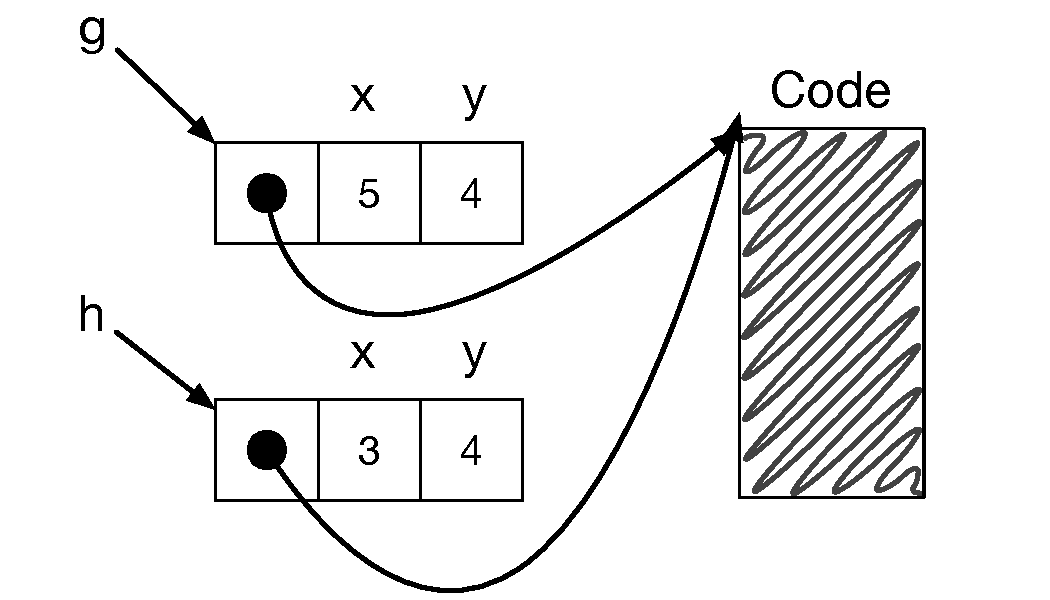
\includegraphics[width=0.6\textwidth]{figs/closures}
\caption{Flat closure representations for the two functions
  produced by the \key{lambda} in Figure~\ref{fig:lexical-scoping}.}
\label{fig:closures}
\end{figure}

Continuing with the example, consider the application of \code{g} to
\code{11} in Figure~\ref{fig:lexical-scoping}.  To apply a closure, we
obtain the function pointer in the first element of the closure and
call it, passing in the closure itself and then the regular arguments,
in this case \code{11}. This technique for applying a closure is step
2 of the dance.
%
But doesn't this \code{lambda} only take 1 argument, for parameter
\code{z}? The third and final step of the dance is generating a
top-level function for a \code{lambda}.  We add an additional
parameter for the closure and we insert an initialization at the beginning
of the function for each free variable, to bind those variables to the
appropriate elements from the closure parameter.
%
This three-step dance is known as \emph{closure conversion}.  We
discuss the details of closure conversion in
Section~\ref{sec:closure-conversion} and the code generated from the
example in Section~\ref{sec:example-lambda}. But first we define the
syntax and semantics of \LangLam{} in Section~\ref{sec:r5}.

\section{The \LangLam{} Language}
\label{sec:r5}

The concrete and abstract syntax for \LangLam{}, a language with anonymous
functions and lexical scoping, is defined in
Figures~\ref{fig:Rlam-concrete-syntax} and \ref{fig:Rlam-syntax}. It adds
the \key{lambda} form to the grammar for \LangFun{}, which already has
syntax for function application. 
%
\python{The syntax also includes an assignment statement that includes
  a type annotation for the variable on the left-hand side, which
  facilitates the type checking of \code{lambda} expressions that we
  discuss later in this section.}
%
\python{The \code{arity} operation returns the number of parameters of
  a given function, an operation that we need for the translation
  of dynamic typing in Chapter~\ref{ch:Ldyn}.
  The \code{arity} operation is not in Python, but the same functionality
  is available in a more complex form. We include \code{arity} in the
  \LangLam{} source language to enable testing.}

\newcommand{\LlambdaGrammarRacket}{
  \begin{array}{lcl}
  \Exp &::=& \LP \key{procedure-arity}~\Exp\RP \\
    &\MID& \CLAMBDA{\LP\LS\Var \key{:} \Type\RS\ldots\RP}{\Type}{\Exp} 
  \end{array}
}
\newcommand{\LlambdaASTRacket}{
  \begin{array}{lcl}
  \itm{op} &::=& \code{procedure-arity} \\
  \Exp &::=& \LAMBDA{\LP\LS\Var\code{:}\Type\RS\ldots\RP}{\Type}{\Exp}
  \end{array}
}

\newcommand{\LlambdaGrammarPython}{
  \begin{array}{lcl}
  \Exp &::=& \CLAMBDA{\Var\code{, }\ldots}{\Exp} \MID \CARITY{\Exp} \\
  \Stmt &::=& \CANNASSIGN{\Var}{\Type}{\Exp}
  \end{array}
}

\newcommand{\LlambdaASTPython}{
  \begin{array}{lcl}
  \Exp &::=& \LAMBDA{\Var^{*}}{\Exp} \MID \ARITY{\Exp} \\
  \Stmt &::=& \ANNASSIGN{\Var}{\Type}{\Exp}
  \end{array}
}


% include AnnAssign in ASTPython

\begin{figure}[tp]
\centering
\fbox{
  \begin{minipage}{0.96\textwidth}
    \small
{\if\edition\racketEd
\[
\begin{array}{l}
  \gray{\LintGrammarRacket{}} \\ \hline
  \gray{\LvarGrammarRacket{}} \\ \hline
  \gray{\LifGrammarRacket{}} \\ \hline
  \gray{\LwhileGrammarRacket} \\ \hline
  \gray{\LtupGrammarRacket} \\   \hline
  \gray{\LfunGrammarRacket} \\   \hline
  \LlambdaGrammarRacket \\
  \begin{array}{lcl}
  \LangLamM{} &::=& \Def\ldots \; \Exp
  \end{array}
\end{array}
\]
\fi}
{\if\edition\pythonEd
\[
\begin{array}{l}
  \gray{\LintGrammarPython{}} \\ \hline
  \gray{\LvarGrammarPython{}} \\ \hline
  \gray{\LifGrammarPython{}} \\ \hline
  \gray{\LwhileGrammarPython} \\ \hline
  \gray{\LtupGrammarPython} \\   \hline
  \gray{\LfunGrammarPython} \\   \hline
  \LlambdaGrammarPython \\
  \begin{array}{lcl}
    \LangFunM{} &::=& \Def\ldots \Stmt\ldots
  \end{array}
\end{array}
\]
\fi}
\end{minipage}
}
\caption{The concrete syntax of \LangLam{}, extending \LangFun{} (Figure~\ref{fig:Rfun-concrete-syntax}) 
  with \key{lambda}.}
\label{fig:Rlam-concrete-syntax}
\end{figure}

\begin{figure}[tp]
\centering
\fbox{
  \begin{minipage}{0.96\textwidth}
    \small
{\if\edition\racketEd
\[
\begin{array}{l}
  \gray{\LintOpAST} \\ \hline
  \gray{\LvarASTRacket{}} \\ \hline
  \gray{\LifASTRacket{}} \\ \hline
  \gray{\LwhileASTRacket{}} \\ \hline
  \gray{\LtupASTRacket{}} \\ \hline
  \gray{\LfunASTRacket} \\ \hline
  \LlambdaASTRacket \\
  \begin{array}{lcl}
  \LangLamM{} &::=& \PROGRAMDEFSEXP{\code{'()}}{\LP\Def\ldots\RP}{\Exp}
  \end{array}
\end{array}
\]
\fi}
{\if\edition\pythonEd
\[
\begin{array}{l}
  \gray{\LintASTPython} \\ \hline
  \gray{\LvarASTPython{}} \\ \hline
  \gray{\LifASTPython{}} \\ \hline
  \gray{\LwhileASTPython{}} \\ \hline
  \gray{\LtupASTPython{}} \\ \hline
  \gray{\LfunASTPython} \\ \hline
  \LlambdaASTPython \\
  \begin{array}{lcl}
  \LangLamM{} &::=& \PROGRAM{}{\LS \Def \ldots \Stmt \ldots \RS}
  \end{array}
\end{array}
\]
\fi}
\end{minipage}
}
\caption{The abstract syntax of \LangLam{}, extending \LangFun{} (Figure~\ref{fig:Rfun-syntax}).}
\label{fig:Rlam-syntax}
\end{figure}

\index{subject}{interpreter}
\label{sec:interp-Rlambda}

Figure~\ref{fig:interp-Rlambda} shows the definitional interpreter for
\LangLam{}. The case for \key{Lambda} saves the current environment
inside the returned function value. Recall that during function
application, the environment stored in the function value, extended
with the mapping of parameters to argument values, is used to
interpret the body of the function.

\begin{figure}[tbp]
{\if\edition\racketEd 
\begin{lstlisting}
(define interp-Rlambda_class
  (class interp-Rfun_class
    (super-new)

    (define/override (interp-op op)
      (match op
        ['procedure-arity
         (lambda (v)
           (match v
             [`(function (,xs ...) ,body ,lam-env)  (length xs)]
             [else (error 'interp-op "expected a function, not ~a" v)]))]
        [else (super interp-op op)]))

    (define/override ((interp-exp env) e)
      (define recur (interp-exp env))
      (match e
        [(Lambda (list `[,xs : ,Ts] ...) rT body)
         `(function ,xs ,body ,env)]
        [else ((super interp-exp env) e)]))
    ))

(define (interp-Rlambda p)
  (send (new interp-Rlambda_class) interp-program p))
\end{lstlisting}
\fi}
{\if\edition\pythonEd
\begin{lstlisting}
class InterpLlambda(InterpLfun):

  def arity(self, v):
    match v:
      case Function(name, params, body, env):
        return len(params)
      case _:
        raise Exception('Llambda arity unexpected ' + repr(v))
      
  def interp_exp(self, e, env):
    match e:
      case Call(Name('arity'), [fun]):
        f = self.interp_exp(fun, env)
        return self.arity(f)
      case Lambda(params, body):
        return Function('lambda', params, [Return(body)], env)
      case _:
        return super().interp_exp(e, env)
    
  def interp_stmts(self, ss, env):
    if len(ss) == 0:
      return
    match ss[0]:
      case AnnAssign(lhs, typ, value, simple):
        env[lhs.id] = self.interp_exp(value, env)
        return self.interp_stmts(ss[1:], env)
      case _:
        return super().interp_stmts(ss, env)
\end{lstlisting}
\fi}
\caption{Interpreter for \LangLam{}.}
\label{fig:interp-Rlambda}
\end{figure}


\label{sec:type-check-r5}
\index{subject}{type checking}

{\if\edition\racketEd
%
Figure~\ref{fig:type-check-Llambda} shows how to type check the new
\key{lambda} form. The body of the \key{lambda} is checked in an
environment that includes the current environment (because it is
lexically scoped) and also includes the \key{lambda}'s parameters.  We
require the body's type to match the declared return type.
%
\fi}

{\if\edition\pythonEd
%
Figures~\ref{fig:type-check-Llambda} and
\ref{fig:type-check-Llambda-part2} define the type checker for
\LangLam{}, which is more complex than one might expect. The reason
for the added complexity is that the syntax of \key{lambda} does not
include type annotations for the parameters or return type.  Instead
they must be inferred. There are many approaches of type inference to
choose from of varying degrees of complexity. We choose one of the
simpler approaches, bidirectional type inference~\citep{Dunfield:2021}
(aka. local type inference~\citep{Pierce:2000}), because the focus of
this book is compilation, not type inference.

The main idea of bidirectional type inference is to add an auxilliary
function, here named \code{check\_exp}, that takes an expected type
and checks whether the given expression is of that type.  Thus, in
\code{check\_exp}, type information flows in a top-down manner with
respect to the AST, in contrast to the regular \code{type\_check\_exp}
function, where type information flows in a primarily bottom-up
manner.
%
The idea then is to use \code{check\_exp} in all the places where we
already know what the type of an expression should be, such as in the
\code{return} statement of a top-level function definition, or on the
right-hand side of an annotated assignment statement.

Getting back to \code{lambda}, it is straightforward to check a
\code{lambda} inside \code{check\_exp} because the expected type
provides the parameter types and the return type.  On the other hand,
inside \code{type\_check\_exp} we disallow \code{lambda}, which means
that we do not allow \code{lambda} in contexts where we don't already
know its type. This restriction does not incur a loss of
expressiveness for \LangLam{} because it is straightforward to modify
a program to sidestep the restriction, for example, by using an
annotated assignment statement to assign the \code{lambda} to a
temporary variable.

Note that for the \code{Name} and \code{Lambda} AST nodes, the type
checker records their type in a \code{has\_type} field. This type
information is used later in this chapter.
%
\fi}

\begin{figure}[tbp]
{\if\edition\racketEd 
\begin{lstlisting}
(define (type-check-Rlambda env)
  (lambda (e)
    (match e
      [(Lambda (and params `([,xs : ,Ts] ...)) rT body)
       (define-values (new-body bodyT) 
          ((type-check-exp (append (map cons xs Ts) env)) body))
       (define ty `(,@Ts -> ,rT))
       (cond
         [(equal? rT bodyT)
           (values (HasType (Lambda params rT new-body) ty) ty)]
         [else
           (error "mismatch in return type" bodyT rT)])]
      ...
      )))
\end{lstlisting}
\fi}
{\if\edition\pythonEd 
\begin{lstlisting}
class TypeCheckLlambda(TypeCheckLfun):

  def type_check_exp(self, e, env):
    match e:
      case Name(id):
        e.has_type = env[id]
        return env[id]
      case Lambda(params, body):
        raise Exception('cannot synthesize a type for a lambda')
      case Call(Name('arity'), [func]):
        func_t = self.type_check_exp(func, env)
        match func_t:
          case FunctionType(params_t, return_t):
            return IntType()
          case _:
            raise Exception('in arity, unexpected ' + repr(func_t))
      case _:
        return super().type_check_exp(e, env)
    
  def check_exp(self, e, ty, env):
    match e:
      case Lambda(params, body):
        e.has_type = ty
        match ty:
          case FunctionType(params_t, return_t):
            new_env = env.copy().update(zip(params, params_t))
            self.check_exp(body, return_t, new_env)
          case _:
            raise Exception('lambda does not have type ' + str(ty))
      case Call(func, args):
        func_t = self.type_check_exp(func, env)
        match func_t:
          case FunctionType(params_t, return_t):
            for (arg, param_t) in zip(args, params_t):
                self.check_exp(arg, param_t, env)
            self.check_type_equal(return_t, ty, e)
          case _:
            raise Exception('type_check_exp: in call, unexpected ' + \
                            repr(func_t))
      case _:
        t = self.type_check_exp(e, env)
        self.check_type_equal(t, ty, e)
\end{lstlisting}
\fi}
\caption{Type checking \LangLam{}\python{, part 1}.}
\label{fig:type-check-Llambda}
\end{figure}


{\if\edition\pythonEd 
\begin{figure}[tbp]
\begin{lstlisting}
  def check_stmts(self, ss, return_ty, env):
    if len(ss) == 0:
      return
    match ss[0]:
      case FunctionDef(name, params, body, dl, returns, comment):
        new_env = env.copy().update(params)
        rt = self.check_stmts(body, returns, new_env)
        self.check_stmts(ss[1:], return_ty, env)
      case Return(value):
        self.check_exp(value, return_ty, env)
      case Assign([Name(id)], value):
        if id in env:
          self.check_exp(value, env[id], env)
        else:
          env[id] = self.type_check_exp(value, env)
        self.check_stmts(ss[1:], return_ty, env)
      case Assign([Subscript(tup, Constant(index), Store())], value):
        tup_t = self.type_check_exp(tup, env)
        match tup_t:
          case TupleType(ts):
            self.check_exp(value, ts[index], env)
          case _:
            raise Exception('expected a tuple, not '  + repr(tup_t))
        self.check_stmts(ss[1:], return_ty, env)
      case AnnAssign(Name(id), ty_annot, value, simple):
        ss[0].annotation = ty_annot
        if id in env:
            self.check_type_equal(env[id], ty_annot)
        else:
            env[id] = ty_annot
        self.check_exp(value, ty_annot, env)
        self.check_stmts(ss[1:], return_ty, env)
      case _:
        self.type_check_stmts(ss, env)

  def type_check(self, p):
    match p:
      case Module(body):
        env = {}
        for s in body:
            match s:
              case FunctionDef(name, params, bod, dl, returns, comment):
                params_t = [t for (x,t) in params]
                env[name] = FunctionType(params_t, returns)
        self.check_stmts(body, int, env)
\end{lstlisting}
\caption{Type checking the \key{lambda}'s in \LangLam{}, part 2.}
\label{fig:type-check-Llambda-part2}
\end{figure}
\fi}

\clearpage

\section{Assignment and Lexically Scoped Functions}
\label{sec:assignment-scoping}

The combination of lexically-scoped functions and assignment to
variables raises a challenge with our approach to implementing
lexically-scoped functions. Consider the following example in which
function \code{f} has a free variable \code{x} that is changed after
\code{f} is created but before the call to \code{f}.
% loop_test_11.rkt
{\if\edition\racketEd
\begin{lstlisting}
(let ([x 0])
  (let ([y 0])
    (let ([z 20])
      (let ([f (lambda: ([a : Integer]) : Integer (+ a (+ x z)))])
        (begin
          (set! x 10)
          (set! y 12)
          (f y))))))
\end{lstlisting}
\fi}
{\if\edition\pythonEd
%  box_free_assign.py
\begin{lstlisting}
def g(z : int) -> int:
    x = 0
    y = 0  
    f : Callable[[int],int] = lambda a: a + x + z
    x = 10
    y = 12
    return f(y)

print( g(20) )
\end{lstlisting}
\fi}
The correct output for this example is \code{42} because the call to
\code{f} is required to use the current value of \code{x} (which is
\code{10}). Unfortunately, the closure conversion pass
(Section~\ref{sec:closure-conversion}) generates code for the
\code{lambda} that copies the old value of \code{x} into a
closure. Thus, if we naively add support for assignment to our current
compiler, the output of this program would be \code{32}.

A first attempt at solving this problem would be to save a pointer to
\code{x} in the closure and change the occurrences of \code{x} inside
the lambda to dereference the pointer. Of course, this would require
assigning \code{x} to the stack and not to a register. However, the
problem goes a bit deeper.
%% Consider the following example in which we
%% create a counter abstraction by creating a pair of functions that
%% share the free variable \code{x}.
Consider the following example that returns a function that refers to
a local variable of the enclosing function.
\begin{center}
\begin{minipage}{\textwidth}
{\if\edition\racketEd
% similar to loop_test_10.rkt
%% \begin{lstlisting}
%% (define (f [x : Integer]) : (Vector ( -> Integer) ( -> Void))
%%   (vector
%%    (lambda: () : Integer x)
%%    (lambda: () : Void (set! x (+ 1 x)))))

%% (let ([counter (f 0)])
%%   (let ([get (vector-ref counter 0)])
%%     (let ([inc (vector-ref counter 1)])
%%       (begin
%%         (inc)
%%         (get)))))
%% \end{lstlisting}
\begin{lstlisting}
(define (f []) : Integer
  (let ([x 0])
    (let ([g (lambda: () : Integer x)])
      (begin
        (set! x 42)
        g))))
((f))
\end{lstlisting}
\fi}
{\if\edition\pythonEd
% counter.py  
\begin{lstlisting}
def f():
    x = 0
    g = lambda: x
    x = 42
    return g

print( f()() )
\end{lstlisting}
\fi}
\end{minipage}
\end{center}
In this example, the lifetime of \code{x} extends beyond the lifetime
of the call to \code{f}. Thus, if we were to store \code{x} on the
stack frame for the call to \code{f}, it would be gone by the time we
call \code{g}, leaving us with dangling pointers for
\code{x}. This example demonstrates that when a variable occurs free
inside a function, its lifetime becomes indefinite. Thus, the value of
the variable needs to live on the heap.  The verb
\emph{box}\index{subject}{box} is often used for allocating a single
value on the heap, producing a pointer, and
\emph{unbox}\index{subject}{unbox} for dereferencing the pointer.

%% {\if\edition\racketEd
%% We recommend solving these problems by boxing the local variables that
%% are in the intersection of 1) variables that appear on the
%% left-hand-side of a \code{set!}  and 2) variables that occur free
%% inside a \code{lambda}.
%% \fi}
%% {\if\edition\pythonEd
%% We recommend solving these problems by boxing the local variables that
%% are in the intersection of 1) variables whose values may change and 2)
%% variables that occur free inside a \code{lambda}.
%% \fi}
We shall introduce a new pass named
\code{convert\_assignments} in Section~\ref{sec:convert-assignments}
to address this challenge.
%
\racket{But before diving into the compiler passes, we have one more
  problem to discuss.}

\if\edition\pythonEd
\section{Uniquify Variables}
\label{sec:uniquify-lambda}

With the addition of \code{lambda} we have a complication to deal
with: name shadowing. Consider the following program with a function
\code{f} that has a parameter \code{x}. Inside \code{f} there are two
\code{lambda} expressions. The first \code{lambda} has a parameter
that is also named \code{x}.

\begin{lstlisting}
def f(x:int, y:int) -> Callable[[int], int]:
  g : Callable[[int],int] = (lambda x: x + y)
  h : Callable[[int],int] = (lambda y: x + y)
  x = input_int()
  return g

print(f(0, 10)(32))
\end{lstlisting}

Many of our compiler passes rely on being able to connect variable
uses with their definitions using just the name of the variable,
including new passes in this chapter. However, in the above example
the name of the variable does not uniquely determine its
definition. To solve this problem we recommend implementing a pass
named \code{uniquify} that renames every variable in the program to
make sure they are all unique.

The following shows the result of \code{uniquify} for the above
example. The \code{x} parameter of \code{f} is renamed to \code{x\_0}
and the \code{x} parameter of the \code{lambda} is renamed to
\code{x\_4}.

\begin{lstlisting}
def f(x_0:int, y_1:int) -> Callable[[int], int] :
  g_2 : Callable[[int], int] = (lambda x_4: x_4 + y_1)
  h_3 : Callable[[int], int] = (lambda y_5: x_0 + y_5)
  x_0 = input_int()
  return g_2

def main() -> int :
  print(f(0, 10)(32))
  return 0
\end{lstlisting}

\fi

%% \section{Reveal Functions}
%% \label{sec:reveal-functions-r5}

%% \racket{To support the \code{procedure-arity} operator we need to
%%   communicate the arity of a function to the point of closure
%%   creation.}
%% %
%% \python{In Chapter~\ref{ch:Ldyn} we need to access the arity of a
%%   function at runtime. Thus, we need to communicate the arity of a
%%   function to the point of closure creation.}
%% %
%% We can accomplish this by replacing the $\FUNREF{\Var}{\Int}$ AST node with
%% one that has a second field for the arity: $\FUNREFARITY{\Var}{\Int}$.
%% \[
%% \begin{array}{lcl}
%% \Exp &::=& \FUNREFARITY{\Var}{\Int}
%% \end{array}
%% \]

\section{Assignment Conversion}
\label{sec:convert-assignments}

The purpose of the \code{convert\_assignments} pass is to address the
challenge posed in Section~\ref{sec:assignment-scoping} regarding the
interaction between variable assignments and closure conversion.
First we identify which variables need to be boxed, then we transform
the program to box those variables. In general, boxing introduces
runtime overhead that we would like to avoid, so we should box as few
variables as possible. We recommend boxing the variables in the
intersection of the following two sets of variables:
\begin{enumerate}
\item The variables that are free in a \code{lambda}.
\item The variables that appear on the left-hand side of an
  assignment.
\end{enumerate}
The first condition is a must, but the second condition is quite conservative and it is possible to
develop a more liberal condition. 

Consider again the first example from
Section~\ref{sec:assignment-scoping}:
%
{\if\edition\racketEd
\begin{lstlisting}
(let ([x 0])
  (let ([y 0])
    (let ([z 20])
      (let ([f (lambda: ([a : Integer]) : Integer (+ a (+ x z)))])
        (begin
          (set! x 10)
          (set! y 12)
          (f y))))))
\end{lstlisting}
\fi}
{\if\edition\pythonEd
\begin{lstlisting}
def g(z : int) -> int:
    x = 0
    y = 0  
    f : Callable[[int],int] = lambda a: a + x + z
    x = 10
    y = 12
    return f(y)

print( g(20) )
\end{lstlisting}
\fi}
%
\noindent The variables \code{x} and \code{y} are assigned-to.  The
variables \code{x} and \code{z} occur free inside the
\code{lambda}. Thus, variable \code{x} needs to be boxed but not
\code{y} or \code{z}.  The boxing of \code{x} consists of three
transformations: initialize \code{x} with a tuple whose elements are uninitialized,
replace reads from \code{x} with tuple reads, and replace each assignment to \code{x}
with a tuple write. The output of \code{convert\_assignments} for
this example is as follows.
%
{\if\edition\racketEd
\begin{lstlisting}
(define (main) : Integer
  (let ([x0 (vector 0)])
    (let ([y1 0])
      (let ([z2 20])
        (let ([f4 (lambda: ([a3 : Integer]) : Integer
                      (+ a3 (+ (vector-ref x0 0) z2)))])
          (begin 
            (vector-set! x0 0 10)
            (set! y1 12)
            (f4 y1)))))))
\end{lstlisting}
\fi}
%
{\if\edition\pythonEd
\begin{lstlisting}
def g(z : int)-> int:
  x = (uninitialized(int),)
  x[0] = 0
  y = 0
  f : Callable[[int], int] = (lambda a: a + x[0] + z)
  x[0] = 10
  y = 12
  return f(y)

def main() -> int:
  print(g(20))
  return 0
\end{lstlisting}
\fi}

To compute the free variables of all the \code{lambda} expressions, we
recommend defining two auxiliary functions:
\begin{enumerate}
\item \code{free\_variables} computes the free variables of an expression, and
\item \code{free\_in\_lambda} collects all of the variables that are
  free in any of the \code{lambda} expressions, using
  \code{free\_variables} in the case for each \code{lambda}.
\end{enumerate}


{\if\edition\racketEd
%
To compute the variables that are assigned-to, we recommend using the
\code{collect-set!} function that we introduced in
Section~\ref{sec:uncover-get-bang}, but updated to include the new AST
forms such as \code{Lambda}.
%
\fi}
  
{\if\edition\pythonEd
%
To compute the variables that are assigned-to, we recommend defining
an auxiliary function named \code{assigned\_vars\_stmt} that returns
the set of variables that occur in the left-hand side of an assignment
statement, and otherwise returns the empty set.
%
\fi}

Let $\mathit{AF}$ be the intersection of the set of variables that are
free in a \code{lambda} and that are assigned-to in the enclosing
function definition.

Next we discuss the \code{convert\_assignments} pass.  In the case for
$\VAR{x}$, if $x$ is in $\mathit{AF}$, then unbox it by translating
$\VAR{x}$ to a tuple read.
%
{\if\edition\racketEd
\begin{lstlisting}
  (Var |$x$|)
  |$\Rightarrow$|
  (Prim 'vector-ref (list (Var |$x$|) (Int 0)))
\end{lstlisting}
\fi}
%
{\if\edition\pythonEd
\begin{lstlisting}
  Name(|$x$|)
  |$\Rightarrow$|
  Subscript(Name(|$x$|), Constant(0), Load())
\end{lstlisting}
\fi}
%
%
In the case for assignment, recursively process the right-hand side
\itm{rhs} to obtain \itm{rhs'}.  If $x$ is in $\mathit{AF}$, translate
the assignment into a tuple-write as follows.
%
{\if\edition\racketEd
\begin{lstlisting}
  (SetBang |$x$| |$\itm{rhs}$|)
  |$\Rightarrow$|
  (Prim 'vector-set! (list (Var |$x$|) (Int 0) |$\itm{rhs'}$|))
\end{lstlisting}
\fi}
{\if\edition\pythonEd
\begin{lstlisting}
  Assign([Name(|$x$|)],|$\itm{rhs}$|)
  |$\Rightarrow$|
  Assign([Subscript(Name(|$x$|), Constant(0), Store())], |$\itm{rhs'}$|)
\end{lstlisting}
\fi}
%
{\if\edition\racketEd
The case for \code{Lambda} is non-trivial, but it is similar to the
case for function definitions, which we discuss next.
\fi}

To translate a function definition, we first compute $\mathit{AF}$,
the intersection of the variables that are free in a \code{lambda} and
that are assigned-to. We then apply assignment conversion to the body
of the function definition. Finally, we box the parameters of this
function definition that are in $\mathit{AF}$. For example,
the parameter \code{x} of the following function \code{g}
needs to be boxed.
{\if\edition\racketEd
\begin{lstlisting}
(define (g [x : Integer]) : Integer
  (let ([f (lambda: ([a : Integer]) : Integer (+ a x))])
    (begin
      (set! x 10)
      (f 32))))
\end{lstlisting}
\fi}
%
{\if\edition\pythonEd
\begin{lstlisting}
def g(x : int) -> int:
  f : Callable[[int],int] = lambda a: a + x
  x = 10
  return f(32)
\end{lstlisting}
\fi}
%
\noindent We box parameter \code{x} by creating a local variable named
\code{x} that is initialized to a tuple whose contents is the value of
the parameter, which we has been renamed.
%
{\if\edition\racketEd
\begin{lstlisting}
(define (g [x_0 : Integer]) : Integer
  (let ([x (vector x_0)])
    (let ([f (lambda: ([a : Integer]) : Integer
               (+ a (vector-ref x 0)))])
      (begin 
        (vector-set! x 0 10)
        (f 32)))))
\end{lstlisting}
\fi}
%
{\if\edition\pythonEd
\begin{lstlisting}
def g(x_0 : int)-> int:
  x = (x_0,)
  f : Callable[[int], int] = (lambda a: a + x[0])
  x[0] = 10
  return f(32)
\end{lstlisting}
\fi}

%% Recall the second example in Section~\ref{sec:assignment-scoping}
%% involving a counter abstraction. The following is the output of
%% assignment version for function \code{f}.
%% \begin{lstlisting}
%% (define (f0 [x1 : Integer]) : (Vector ( -> Integer) ( -> Void))
%%   (vector
%%    (lambda: () : Integer x1)
%%    (lambda: () : Void (set! x1 (+ 1 x1)))))
%% |$\Rightarrow$|
%% (define (f0 [param_x1 : Integer]) : (Vector (-> Integer) (-> Void))
%%   (let ([x1 (vector param_x1)])
%%     (vector (lambda: () : Integer (vector-ref x1 0))
%%              (lambda: () : Void
%%                 (vector-set! x1 0 (+ 1 (vector-ref x1 0)))))))
%% \end{lstlisting}

\section{Closure Conversion}
\label{sec:closure-conversion}
\index{subject}{closure conversion}

The compiling of lexically-scoped functions into top-level function
definitions is accomplished in the pass \code{convert\_to\_closures}
that comes after \code{reveal\_functions} and before
\code{limit\_functions}. 

As usual, we implement the pass as a recursive function over the
AST. The interesting cases are the ones for \key{lambda} and function
application. We transform a \key{lambda} expression into an expression
that creates a closure, that is, a tuple whose first element is a
function pointer and the rest of the elements are the values of the
free variables of the \key{lambda}.
%
However, we use the \code{Closure} AST node instead of using a tuple
so that we can record the arity.
%
In the generated code below, \itm{fvs} is the free variables of the
lambda and \itm{name} is a unique symbol generated to identify the lambda.
%
\racket{The \itm{arity} is the number of parameters (the length of
  \itm{ps}).}
%
{\if\edition\racketEd
\begin{lstlisting}
(Lambda |\itm{ps}| |\itm{rt}| |\itm{body}|)
|$\Rightarrow$|
(Closure |\itm{arity}| (cons (FunRef |\itm{name}| |\itm{arity}|) |\itm{fvs}|))
\end{lstlisting}
\fi}
%
{\if\edition\pythonEd
\begin{lstlisting}
Lambda([|$x_1,\ldots,x_n$|], |\itm{body}|)
|$\Rightarrow$|
Closure(|$n$|, [FunRef(|\itm{name}|, |$n$|), |\itm{fvs}, \ldots|])
\end{lstlisting}
\fi}
%
In addition to transforming each \key{Lambda} AST node into a
tuple, we create a top-level function definition for each
\key{Lambda}, as shown below.\\
\begin{minipage}{0.8\textwidth}
{\if\edition\racketEd
\begin{lstlisting}
(Def |\itm{name}| ([clos : (Vector _ |\itm{fvts}| ...)] |\itm{ps'}| ...) |\itm{rt'}|
   (Let |$\itm{fvs}_1$| (Prim 'vector-ref (list (Var clos) (Int 1)))
     ...
     (Let |$\itm{fvs}_n$| (Prim 'vector-ref (list (Var clos) (Int |$n$|)))
       |\itm{body'}|)...))
\end{lstlisting}
\fi}
{\if\edition\pythonEd
\begin{lstlisting}
def |\itm{name}|(clos : |\itm{closTy}|, |\itm{ps'}, \ldots|) -> |\itm{rt'}|:
   |$\itm{fvs}_1$| = clos[1]
   |$\ldots$|
   |$\itm{fvs}_n$| = clos[|$n$|]
   |\itm{body'}|
\end{lstlisting}
\fi}
\end{minipage}\\
The \code{clos} parameter refers to the closure.  Translate the type
annotations in \itm{ps} and the return type \itm{rt}, as discussed in
the next paragraph, to obtain \itm{ps'} and \itm{rt'}.  The type
\itm{closTy} is a tuple type whose first element type is
\python{\code{Bottom()}}\racket{\code{\_} (the dummy type)} and the rest of
the element types are the types of the free variables in the
lambda. We use \python{\code{Bottom()}}\racket{\code{\_}} because it
is non-trivial to give a type to the function in the closure's type.%
%
\footnote{To give an accurate type to a closure, we would need to add
  existential types to the type checker~\citep{Minamide:1996ys}.}
%
%% The dummy type is considered to be equal to any other type during type
%% checking.
The free variables become local variables that are initialized with
their values in the closure.

Closure conversion turns every function into a tuple, so the type
annotations in the program must also be translated.  We recommend
defining an auxiliary recursive function for this purpose.  Function
types should be translated as follows.
%
{\if\edition\racketEd
\begin{lstlisting}
(|$T_1, \ldots, T_n$| -> |$T_r$|)
|$\Rightarrow$|  
(Vector ((Vector) |$T'_1, \ldots, T'_n$| -> |$T'_r$|))
\end{lstlisting}
\fi}
{\if\edition\pythonEd
\begin{lstlisting}
FunctionType([|$T_1, \ldots, T_n$|], |$T_r$|)
|$\Rightarrow$|  
TupleType([FunctionType([TupleType([]), |$T'_1, \ldots, T'_n$|], |$T'_r$|)])
\end{lstlisting}
\fi}
%
The above type says that the first thing in the tuple is a
function. The first parameter of the function is a tuple (a closure)
and the rest of the parameters are the ones from the original
function, with types $T'_1, \ldots, T'_n$.  The type for the closure
omits the types of the free variables because 1) those types are not
available in this context and 2) we do not need them in the code that
is generated for function application. So this type only describes the
first component of the closure tuple. At runtime the tuple may have
more components, but we ignore them at this point.

We transform function application into code that retrieves the
function from the closure and then calls the function, passing the
closure as the first argument. We place $e'$ in a temporary variable
to avoid code duplication.
\begin{center}
\begin{minipage}{\textwidth}
{\if\edition\racketEd
\begin{lstlisting}
(Apply |$e$| |$\itm{es}$|)
|$\Rightarrow$|
(Let |$\itm{tmp}$| |$e'$|
  (Apply (Prim 'vector-ref (list (Var |$\itm{tmp}$|) (Int 0))) (cons |$\itm{tmp}$| |$\itm{es'}$|)))
\end{lstlisting}
\fi}
%
{\if\edition\pythonEd
\begin{lstlisting}
Call(|$e$|, [|$e_1, \ldots, e_n$|])
|$\Rightarrow$|
Begin([Assign([|$\itm{tmp}$|], |$e'$|)],
      Call(Subscript(Name(|$\itm{tmp}$|), Constant(0)),
           [|$\itm{tmp}$|, |$e'_1, \ldots, e'_n$|]))
\end{lstlisting}
\fi}
\end{minipage}
\end{center}

There is also the question of what to do with references to top-level
function definitions. To maintain a uniform translation of function
application, we turn function references into closures.

\begin{tabular}{lll}
\begin{minipage}{0.3\textwidth}
{\if\edition\racketEd
\begin{lstlisting}
(FunRef |$f$| |$n$|)
\end{lstlisting}
\fi}
{\if\edition\pythonEd
\begin{lstlisting}
FunRef(|$f$|, |$n$|)
\end{lstlisting}
\fi}
\end{minipage}
&
$\Rightarrow$
&
\begin{minipage}{0.5\textwidth}
{\if\edition\racketEd
\begin{lstlisting}
(Closure |$n$| (FunRef |$f$| |$n$|) '())
\end{lstlisting}
\fi}
{\if\edition\pythonEd
\begin{lstlisting}
Closure(|$n$|, [FunRef(|$f$| |$n$|)])
\end{lstlisting}
\fi}
\end{minipage}
\end{tabular}  \\


We no longer need the annotated assignment statement \code{AnnAssign}
to support the type checking of \code{lambda} expressions, so we
translate it to a regular \code{Assign} statement.

The top-level function definitions need to be updated to take an extra
closure parameter.

\section{An Example Translation}
\label{sec:example-lambda}

Figure~\ref{fig:lexical-functions-example} shows the result of
\code{reveal\_functions} and \code{convert\_to\_closures} for the example
program demonstrating lexical scoping that we discussed at the
beginning of this chapter.


\begin{figure}[tbp]
  \begin{minipage}{0.8\textwidth}
{\if\edition\racketEd
% tests/lambda_test_6.rkt
\begin{lstlisting}[basicstyle=\ttfamily\footnotesize]
(define (f6 [x7 : Integer]) : (Integer -> Integer)
   (let ([y8 4])
      (lambda: ([z9 : Integer]) : Integer
         (+ x7 (+ y8 z9)))))

(define (main) : Integer
   (let ([g0 ((fun-ref f6 1) 5)])
      (let ([h1 ((fun-ref f6 1) 3)])
         (+ (g0 11) (h1 15)))))
\end{lstlisting}
$\Rightarrow$
\begin{lstlisting}[basicstyle=\ttfamily\footnotesize]
(define (f6 [fvs4 : _] [x7 : Integer]) : (Vector ((Vector _) Integer -> Integer))
   (let ([y8 4])
      (closure 1 (list (fun-ref lambda2 1) x7 y8))))

(define (lambda2 [fvs3 : (Vector _ Integer Integer)] [z9 : Integer]) : Integer
   (let ([x7 (vector-ref fvs3 1)])
      (let ([y8 (vector-ref fvs3 2)])
         (+ x7 (+ y8 z9)))))

(define (main) : Integer
   (let ([g0 (let ([clos5 (closure 1 (list (fun-ref f6 1)))])
                    ((vector-ref clos5 0) clos5 5))])
      (let ([h1 (let ([clos6 (closure 1 (list (fun-ref f6 1)))])
                       ((vector-ref clos6 0) clos6 3))])
         (+ ((vector-ref g0 0) g0 11) ((vector-ref h1 0) h1 15)))))
\end{lstlisting}
\fi}
%
{\if\edition\pythonEd
% free_var.py
\begin{lstlisting}
def f(x : int) -> Callable[[int], int]:
  y = 4
  return lambda z: x + y + z

g = f(5)
h = f(3)
print( g(11) + h(15) )
\end{lstlisting}
$\Rightarrow$
\begin{lstlisting}
def lambda_0(fvs_1:tuple[bot,int,tuple[int]],z:int) -> int:
  x = fvs_1[1]
  y = fvs_1[2]
  return x + y[0] + z

def f(fvs_2:bot, x:int) -> tuple[Callable[[tuple[],int], int]]
  y = (777,)
  y[0] = 4
  return (lambda_0, x, y)

def main() -> int:
  g = (let clos_3 = (f,) in clos_3[0](clos_3, 5))
  h = (let clos_4 = (f,) in clos_4[0](clos_4, 3))
  print((let clos_5 = g in clos_5[0](clos_5, 11))
        + (let clos_6 = h in clos_6[0](clos_6, 15)))
  return 0
\end{lstlisting}
\fi}
\end{minipage}
\caption{Example of closure conversion.}
\label{fig:lexical-functions-example}
\end{figure}

\begin{exercise}\normalfont\normalsize
Expand your compiler to handle \LangLam{} as outlined in this chapter.
Create 5 new programs that use \key{lambda} functions and make use of
lexical scoping. Test your compiler on these new programs and all of
your previously created test programs.
\end{exercise}

\section{Expose Allocation}
\label{sec:expose-allocation-r5}

Compile the $\CLOSURE{\itm{arity}}{\Exp^{*}}$ form into code
that allocates and initializes a tuple, similar to the translation of
the tuple creation in Section~\ref{sec:expose-allocation}.
The only difference is replacing the use of
\ALLOC{\itm{len}}{\itm{type}} with
\ALLOCCLOS{\itm{len}}{\itm{type}}{\itm{arity}}.


\section{Explicate Control and \LangCLam{}}
\label{sec:explicate-r5}

The output language of \code{explicate\_control} is \LangCLam{} whose
abstract syntax is defined in Figure~\ref{fig:Clam-syntax}.
%
\racket{The only difference with respect to \LangCFun{} is the
  addition of the \code{AllocateClosure} form to the grammar for
  $\Exp$.  The handling of \code{AllocateClosure} in the
  \code{explicate\_control} pass is similar to the handling of other
  expressions such as primitive operators.}
%
\python{The differences with respect to \LangCFun{} are the
  additions of \code{Uninitialized}, \code{AllocateClosure},
  and \code{arity} to the grammar for $\Exp$.  The handling of them in the
  \code{explicate\_control} pass is similar to the handling of other
  expressions such as primitive operators.}

\newcommand{\ClambdaASTPython}{
\begin{array}{lcl}
\Exp &::=& \key{Uninitialized}\LP \Type \RP
      \MID \key{AllocateClosure}\LP\itm{len},\Type, \itm{arity}\RP \\
      &\MID& \ARITY{\Atm}
\end{array}
}

\begin{figure}[tp]
\fbox{
\begin{minipage}{0.96\textwidth}
\small
{\if\edition\racketEd
\[
\begin{array}{lcl}
\Exp &::= & \ldots
   \MID \ALLOCCLOS{\Int}{\Type}{\Int} \\
\Stmt &::=& \gray{ \ASSIGN{\VAR{\Var}}{\Exp} 
       \MID \LP\key{Collect} \,\itm{int}\RP } \\
\Tail &::= & \gray{ \RETURN{\Exp} \MID \SEQ{\Stmt}{\Tail} 
       \MID \GOTO{\itm{label}} } \\
    &\MID& \gray{ \IFSTMT{\BINOP{\itm{cmp}}{\Atm}{\Atm}}{\GOTO{\itm{label}}}{\GOTO{\itm{label}}}  }\\
    &\MID& \gray{ \TAILCALL{\Atm}{\Atm\ldots} } \\
\Def &::=& \gray{ \DEF{\itm{label}}{\LP[\Var\key{:}\Type]\ldots\RP}{\Type}{\itm{info}}{\LP\LP\itm{label}\,\key{.}\,\Tail\RP\ldots\RP} }\\
\LangCLamM{} & ::= & \gray{ \PROGRAMDEFS{\itm{info}}{\LP\Def\ldots\RP} }
\end{array}
\]
\fi}
{\if\edition\pythonEd
\[
  \begin{array}{l}
  \gray{\CifASTPython} \\ \hline
  \gray{\CtupASTPython} \\ \hline
  \gray{\CfunASTPython} \\ \hline
  \ClambdaASTPython \\
  \begin{array}{lcl}
    \LangCLamM{} & ::= & \CPROGRAMDEFS{\LS\Def\code{,}\ldots\RS} 
  \end{array}
  \end{array}
\]
\fi}
\end{minipage}
}
\caption{The abstract syntax of \LangCLam{}, extending \LangCFun{} (Figure~\ref{fig:c3-syntax}).}
\label{fig:Clam-syntax}
\end{figure}


\section{Select Instructions}
\label{sec:select-instructions-Rlambda}

Compile \ALLOCCLOS{\itm{len}}{\itm{type}}{\itm{arity}} in almost the
same way as the \ALLOC{\itm{len}}{\itm{type}} form
(Section~\ref{sec:select-instructions-gc}). The only difference is
that you should place the \itm{arity} in the tag that is stored at
position $0$ of the vector. Recall that in
Section~\ref{sec:select-instructions-gc} a portion of the 64-bit tag
was not used. We store the arity in the $5$ bits starting at position
$58$.

\racket{Compile the \code{procedure-arity} operator into a sequence of
instructions that access the tag from position $0$ of the vector and
extract the $5$-bits starting at position $58$ from the tag.}
%
\python{Compile a call to the \code{arity} operator to a sequence of
instructions that access the tag from position $0$ of the tuple
(representing a closure) and extract the $5$-bits starting at position
$58$ from the tag.}



\begin{figure}[p]
\begin{tikzpicture}[baseline=(current  bounding  box.center)]
\node (Rfun) at (0,2)  {\large \LangLam{}};
\node (Rfun-2) at (3,2)  {\large \LangLam{}};
\node (Rfun-3) at (6,2)  {\large \LangLam{}};
\node (F1-0) at (9,2)  {\large \LangLamFunRef{}};
\node (F1-1) at (12,0)  {\large \LangLamFunRef{}};
\node (F1-2) at (9,0)  {\large \LangFunRef{}};
\node (F1-3) at (6,0)  {\large \LangFunRef{}};
\node (F1-4) at (3,0)  {\large \LangFunRefAlloc{}};
\node (F1-5) at (0,0)  {\large \LangFunANF{}};
\node (C3-2) at (3,-2)  {\large \LangCFun{}};

\node (x86-2) at (3,-4)  {\large \LangXIndCallVar{}};
\node (x86-2-1) at (3,-6)  {\large \LangXIndCallVar{}};
\node (x86-2-2) at (6,-6)  {\large \LangXIndCallVar{}};
\node (x86-3) at (6,-4)  {\large \LangXIndCallVar{}};
\node (x86-4) at (9,-4) {\large \LangXIndCall{}};
\node (x86-5) at (9,-6) {\large \LangXIndCall{}};

\path[->,bend left=15] (Rfun) edge [above] node
     {\ttfamily\footnotesize shrink} (Rfun-2);
\path[->,bend left=15] (Rfun-2) edge [above] node
     {\ttfamily\footnotesize uniquify} (Rfun-3);
\path[->,bend left=15] (Rfun-3) edge [above] node
     {\ttfamily\footnotesize reveal\_functions} (F1-0);
\path[->,bend left=15] (F1-0) edge [right] node
     {\ttfamily\footnotesize convert\_assign.} (F1-1);
\path[->,bend left=15] (F1-1) edge [below] node
     {\ttfamily\footnotesize convert\_to\_clos.} (F1-2);
\path[->,bend right=15] (F1-2) edge [above] node
     {\ttfamily\footnotesize limit\_fun.} (F1-3);
\path[->,bend right=15] (F1-3) edge [above] node
     {\ttfamily\footnotesize expose\_alloc.} (F1-4);
\path[->,bend right=15] (F1-4) edge [above] node
     {\ttfamily\footnotesize remove\_complex.} (F1-5);
\path[->,bend right=15] (F1-5) edge [right] node
     {\ttfamily\footnotesize explicate\_control} (C3-2);
\path[->,bend left=15] (C3-2) edge [left] node
     {\ttfamily\footnotesize select\_instr.} (x86-2);
\path[->,bend right=15] (x86-2) edge [left] node
     {\ttfamily\footnotesize uncover\_live} (x86-2-1);
\path[->,bend right=15] (x86-2-1) edge [below] node 
     {\ttfamily\footnotesize build\_inter.} (x86-2-2);
\path[->,bend right=15] (x86-2-2) edge [left] node
     {\ttfamily\footnotesize allocate\_reg.} (x86-3);
\path[->,bend left=15] (x86-3) edge [above] node
     {\ttfamily\footnotesize patch\_instr.} (x86-4);
\path[->,bend left=15] (x86-4) edge [right] node
     {\ttfamily\footnotesize print\_x86} (x86-5);
\end{tikzpicture}
  \caption{Diagram of the passes for \LangLam{}, a language with lexically-scoped
  functions.}
\label{fig:Rlambda-passes}
\end{figure}

Figure~\ref{fig:Rlambda-passes} provides an overview of all the passes needed
for the compilation of \LangLam{}.

\clearpage

\section{Challenge: Optimize Closures}
\label{sec:optimize-closures}

In this chapter we compiled lexically-scoped functions into a
relatively efficient representation: flat closures. However, even this
representation comes with some overhead. For example, consider the
following program with a function \code{tail\_sum} that does not have
any free variables and where all the uses of \code{tail\_sum} are in
applications where we know that only \code{tail\_sum} is being applied
(and not any other functions).
\begin{center}
\begin{minipage}{0.95\textwidth}
{\if\edition\racketEd  
\begin{lstlisting}
(define (tail_sum [n : Integer] [s : Integer]) : Integer
  (if (eq? n 0)
      s
      (tail_sum (- n 1) (+ n s))))

(+ (tail_sum 3 0) 36)
\end{lstlisting}
\fi}
{\if\edition\pythonEd
\begin{lstlisting}
def tail_sum(n : int, s : int) -> int:
    if n == 0:
        return s
    else:
        return tail_sum(n - 1, n + s)

print( tail_sum(3, 0) + 36)
\end{lstlisting}
\fi}
\end{minipage}
\end{center}
As described in this chapter, we uniformly apply closure conversion to
all functions, obtaining the following output for this program.
\begin{center}
\begin{minipage}{0.95\textwidth}
{\if\edition\racketEd  
\begin{lstlisting}
(define (tail_sum1 [fvs5 : _] [n2 : Integer] [s3 : Integer]) : Integer
   (if (eq? n2 0)
      s3
      (let ([clos4 (closure (list (fun-ref tail_sum1 2)))])
         ((vector-ref clos4 0) clos4 (+ n2 -1) (+ n2 s3)))))

(define (main) : Integer
   (+ (let ([clos6 (closure (list (fun-ref tail_sum1 2)))])
         ((vector-ref clos6 0) clos6 3 0)) 27))
\end{lstlisting}
\fi}
{\if\edition\pythonEd
\begin{lstlisting}
def tail_sum(fvs_3:bot,n_0:int,s_1:int) -> int :
  if n_0 == 0:
    return s_1
  else:
    return (let clos_2 = (tail_sum,)
            in clos_2[0](clos_2, n_0 - 1, n_0 + s_1))

def main() -> int :
  print((let clos_4 = (tail_sum,)
         in clos_4[0](clos_4, 3, 0)) + 36)
  return 0
\end{lstlisting}
\fi}
\end{minipage}
\end{center}

In the previous chapter, there would be no allocation in the program
and the calls to \code{tail\_sum} would be direct calls. In contrast,
the above program allocates memory for each closure and the calls to
\code{tail\_sum} are indirect. These two differences incur
considerable overhead in a program such as this one, where the
allocations and indirect calls occur inside a tight loop.

One might think that this problem is trivial to solve: can't we just
recognize calls of the form \APPLY{\FUNREF{$f$}{$n$}}{$\mathit{args}$}
and compile them to direct calls instead of treating it like a call to
a closure? We would also drop the new \code{fvs} parameter of
\code{tail\_sum}.
%
However, this problem is not so trivial because a global function may
``escape'' and become involved in applications that also involve
closures. Consider the following example in which the application
\CAPPLY{\code{f}}{\code{41}} needs to be compiled into a closure
application, because the \code{lambda} may flow into \code{f}, but the
\code{inc} function might also flow into \code{f}.
\begin{center}
\begin{minipage}{\textwidth}
% lambda_test_30.rkt
{\if\edition\racketEd  
\begin{lstlisting}
(define (inc [x : Integer]) : Integer
  (+ x 1))

(let ([y (read)])
  (let ([f (if (eq? (read) 0)
               inc
               (lambda: ([x : Integer]) : Integer (- x y)))])
    (f 41)))
\end{lstlisting}
\fi}
{\if\edition\pythonEd  
\begin{lstlisting}
def add1(x : int) -> int:
  return x + 1

y = input_int()
g : Callable[[int], int] = lambda x: x - y
f = add1 if input_int() == 0 else g
print( f(41) )
\end{lstlisting}
\fi}
\end{minipage}
\end{center}
If a global function name is used in any way other than as the
operator in a direct call, then we say that the function
\emph{escapes}. If a global function does not escape, then we do not
need to perform closure conversion on the function.

\begin{exercise}\normalfont\normalsize
  Implement an auxiliary function for detecting which global
  functions escape. Using that function, implement an improved version
  of closure conversion that does not apply closure conversion to
  global functions that do not escape but instead compiles them as
  regular functions. Create several new test cases that check whether
  you properly detect whether global functions escape or not.
\end{exercise}

So far we have reduced the overhead of calling global functions, but
it would also be nice to reduce the overhead of calling a
\code{lambda} when we can determine at compile time which
\code{lambda} will be called. We refer to such calls as \emph{known
  calls}.  Consider the following example in which a \code{lambda} is
bound to \code{f} and then applied.
{\if\edition\racketEd
% lambda_test_9.rkt  
\begin{lstlisting}
(let ([y (read)])
  (let ([f (lambda: ([x : Integer]) : Integer
             (+ x y))])
    (f 21)))
\end{lstlisting}
\fi}
{\if\edition\pythonEd
\begin{lstlisting}
y = input_int()
f : Callable[[int],int] = lambda x: x + y
print( f(21) )
\end{lstlisting}
\fi}
%
\noindent Closure conversion compiles the application
\CAPPLY{\code{f}}{\code{21}} into an indirect call:
%
{\if\edition\racketEd
\begin{lstlisting}
(define (lambda5 [fvs6 : (Vector _ Integer)] [x3 : Integer]) : Integer
   (let ([y2 (vector-ref fvs6 1)])
      (+ x3 y2)))

(define (main) : Integer
   (let ([y2 (read)])
      (let ([f4 (Closure 1 (list (fun-ref lambda5 1) y2))])
         ((vector-ref f4 0) f4 21))))
\end{lstlisting}
\fi}
{\if\edition\pythonEd
\begin{lstlisting}
def lambda_3(fvs_4:tuple[bot,tuple[int]], x_2:int) -> int:
  y_1 = fvs_4[1]
  return x_2 + y_1[0]

def main() -> int:
  y_1 = (777,)
  y_1[0] = input_int()
  f_0 = (lambda_3, y_1)
  print((let clos_5 = f_0 in clos_5[0](clos_5, 21)))
  return 0
\end{lstlisting}
\fi}
%
\noindent but we can instead compile the application
\CAPPLY{\code{f}}{\code{21}} into a direct call:
%
{\if\edition\racketEd
\begin{lstlisting}
(define (main) : Integer
   (let ([y2 (read)])
      (let ([f4 (Closure 1 (list (fun-ref lambda5 1) y2))])
         ((fun-ref lambda5 1) f4 21))))
\end{lstlisting}
\fi}
{\if\edition\pythonEd
\begin{lstlisting}
def main() -> int:
  y_1 = (777,)
  y_1[0] = input_int()
  f_0 = (lambda_3, y_1)
  print(lambda_3(f_0, 21))
  return 0
\end{lstlisting}
\fi}

The problem of determining which \code{lambda} will be called from a
particular application is quite challenging in general and the topic
of considerable research~\citep{Shivers:1988aa,Gilray:2016aa}. For the
following exercise we recommend that you compile an application to a
direct call when the operator is a variable and \racket{the variable
  is \code{let}-bound to a closure} \python{the previous assignment to
  the variable is a closure}.  This can be accomplished by maintaining
an environment mapping variables to function names.  Extend the
environment whenever you encounter a closure on the right-hand side of
a \racket{\code{let}}\python{assignment}, mapping the variable to the
name of the global function for the closure. This pass should come
after closure conversion.

\begin{exercise}\normalfont\normalsize
Implement a compiler pass, named \code{optimize\_known\_calls}, that
compiles known calls into direct calls. Verify that your compiler is
successful in this regard on several example programs.
\end{exercise}

These exercises only scratches the surface of optimizing of
closures. A good next step for the interested reader is to look at the
work of \citet{Keep:2012ab}.

\section{Further Reading}

The notion of lexically scoped functions predates modern computers by
about a decade. They were invented by \citet{Church:1932aa}, who
proposed the lambda calculus as a foundation for logic. Anonymous
functions were included in the LISP~\citep{McCarthy:1960dz}
programming language but were initially dynamically scoped. The Scheme
dialect of LISP adopted lexical scoping and
\citet{Guy-L.-Steele:1978yq} demonstrated how to efficiently compile
Scheme programs. However, environments were represented as linked
lists, so variable lookup was linear in the size of the
environment. In this chapter we represent environments using flat
closures, which were invented by
\citet{Cardelli:1983aa,Cardelli:1984aa} for the purposes of compiling
the ML language~\citep{Gordon:1978aa,Milner:1990fk}. With flat
closures, variable lookup is constant time but the time to create a
closure is proportional to the number of its free variables.  Flat
closures were reinvented by \citet{Dybvig:1987ab} in his Ph.D. thesis
and used in Chez Scheme version 1~\citep{Dybvig:2006aa}.


%%%%%%%%%%%%%%%%%%%%%%%%%%%%%%%%%%%%%%%%%%%%%%%%%%%%%%%%%%%%%%%%%%%%%%%%%%%%%%%%
\chapter{Dynamic Typing}
\label{ch:Ldyn}
\index{subject}{dynamic typing}

In this chapter we discuss the compilation of \LangDyn{}, a
dynamically typed language that is a subset of
\racket{Racket}\python{Python}. The dynamic typing is in contrast to
the previous chapters, which have studied the compilation of
statically typed languages. In dynamically typed languages such as
\LangDyn{}, a particular expression may produce a value of a different
type each time it is executed. Consider the following example with a
conditional \code{if} expression that may return a Boolean or an
integer depending on the input to the program.
% part of  dynamic_test_25.rkt
{\if\edition\racketEd
\begin{lstlisting}
(not (if (eq? (read) 1) #f 0))
\end{lstlisting}
\fi}
{\if\edition\pythonEd
\begin{lstlisting}
not (False if input_int() == 1 else 0)
\end{lstlisting}
\fi}

Languages that allow expressions to produce different kinds of values
are called \emph{polymorphic}, a word composed of the Greek roots
``poly'', meaning ``many'', and ``morphos'', meaning ``form''.  There
are several kinds of polymorphism in programming languages, such as
subtype polymorphism and parametric
polymorphism~\citep{Cardelli:1985kx}. The kind of polymorphism we
study in this chapter does not have a special name but it is the kind
that arises in dynamically typed languages.

Another characteristic of dynamically typed languages is that
primitive operations, such as \code{not}, are often defined to operate
on many different types of values.  In fact, in
\racket{Racket}\python{Python}, the \code{not} operator produces a
result for any kind of value: given \FALSE{} it returns \TRUE{} and
given anything else it returns \FALSE{}.

Furthermore, even when primitive operations restrict their inputs to
values of a certain type, this restriction is enforced at runtime
instead of during compilation. For example, the tuple read
operation
\racket{\code{(vector-ref \#t 0)}}
\python{\code{True[0]}}
results in a run-time error because the first argument must
be a tuple, not a Boolean.

\begin{figure}[tp]
\centering
\fbox{
  \begin{minipage}{0.97\textwidth}
{\if\edition\racketEd    
\[
\begin{array}{rcl}
  \itm{cmp} &::= & \key{eq?} \MID \key{<} \MID \key{<=} \MID \key{>} \MID \key{>=} \\
\Exp &::=& \Int \MID \CREAD{} \MID \CNEG{\Exp}
      \MID \CADD{\Exp}{\Exp} \MID \CSUB{\Exp}{\Exp}  \\
     &\MID&  \Var \MID \CLET{\Var}{\Exp}{\Exp} \\
     &\MID& \key{\#t} \MID \key{\#f} 
      \MID \CBINOP{\key{and}}{\Exp}{\Exp} 
     \MID \CBINOP{\key{or}}{\Exp}{\Exp} 
     \MID \CUNIOP{\key{not}}{\Exp} \\
     &\MID& \LP\itm{cmp}\;\Exp\;\Exp\RP \MID \CIF{\Exp}{\Exp}{\Exp} \\
     &\MID& \LP\key{vector}\;\Exp\ldots\RP \MID
      \LP\key{vector-ref}\;\Exp\;\Exp\RP \\
     &\MID& \LP\key{vector-set!}\;\Exp\;\Exp\;\Exp\RP \MID \LP\key{void}\RP \\
      &\MID& \LP\Exp \; \Exp\ldots\RP
      \MID \LP\key{lambda}\;\LP\Var\ldots\RP\;\Exp\RP \\
     & \MID & \LP\key{boolean?}\;\Exp\RP \MID \LP\key{integer?}\;\Exp\RP\\
     & \MID & \LP\key{vector?}\;\Exp\RP \MID \LP\key{procedure?}\;\Exp\RP \MID \LP\key{void?}\;\Exp\RP \\
  \Def &::=& \LP\key{define}\; \LP\Var \; \Var\ldots\RP \; \Exp\RP \\
\LangDynM{}  &::=& \Def\ldots\; \Exp
\end{array}
\]
\fi}
{\if\edition\pythonEd
\[
\begin{array}{rcl}
  \itm{cmp} &::= & \key{==} \MID \key{!=} \MID \key{<} \MID \key{<=} \MID \key{>} \MID \key{>=} \MID \key{is} \\
  \Exp &::=& \Int \MID \key{input\_int}\LP\RP \MID \key{-}\;\Exp \MID \Exp \; \key{+} \; \Exp \MID \Exp \; \key{-} \; \Exp \MID \LP\Exp\RP \\
  &\MID& \Var{} \MID \TRUE \MID \FALSE \MID \CAND{\Exp}{\Exp}
  \MID \COR{\Exp}{\Exp} \MID \key{not}~\Exp \\
  &\MID& \CCMP{\itm{cmp}}{\Exp}{\Exp}
      \MID \CIF{\Exp}{\Exp}{\Exp} \\
  &\MID& \Exp \key{,} \ldots \key{,} \Exp \MID \CGET{\Exp}{\Exp}
      \MID \CLEN{\Exp}  \\
   &\MID& \CAPPLY{\Exp}{\Exp\code{,} \ldots} 
    \MID \CLAMBDA{\Var\code{, }\ldots}{\Exp}\\
  \Stmt &::=& \key{print}\LP \Exp \RP \MID \Exp 
    \MID \Var\mathop{\key{=}}\Exp \\
   &\MID& \key{if}~ \Exp \key{:}~ \Stmt^{+} ~\key{else:}~ \Stmt^{+} 
   \MID \key{while}~ \Exp \key{:}~ \Stmt^{+} \\
    &\MID& \CRETURN{\Exp} \\
   \Def &::=& \CDEFU{\Var}{\Var{,} \ldots}{\Stmt^{+}} \\
  \LangDynM{} &::=& \Def\ldots \Stmt\ldots
\end{array}
\]
\fi}
\end{minipage}
}
\caption{Syntax of \LangDyn{}, an untyped language (a subset of \racket{Racket}\python{Python}).}
\label{fig:r7-concrete-syntax}
\end{figure}


\begin{figure}[tp]
\centering
\fbox{
  \begin{minipage}{0.96\textwidth}
    \small
{\if\edition\racketEd
\[
\begin{array}{lcl}
  \Exp &::=& \INT{\Int} \MID \VAR{\Var} \MID \LET{\Var}{\Exp}{\Exp} \\
       &\MID& \PRIM{\itm{op}}{\Exp\ldots} \\
     &\MID& \BOOL{\itm{bool}}
      \MID \IF{\Exp}{\Exp}{\Exp}  \\
     &\MID& \VOID{} \MID \APPLY{\Exp}{\Exp\ldots} \\
     &\MID& \LAMBDA{\LP\Var\ldots\RP}{\code{'Any}}{\Exp}\\
 \Def &::=& \FUNDEF{\Var}{\LP\Var\ldots\RP}{\code{'Any}}{\code{'()}}{\Exp} \\
  \LangDynM{} &::=& \PROGRAMDEFSEXP{\code{'()}}{\LP\Def\ldots\RP}{\Exp} 
\end{array}
\]
\fi}
{\if\edition\pythonEd
\[
\begin{array}{rcl}
\itm{binaryop} &::= & \code{Add()} \MID \code{Sub()} \\
\itm{unaryop} &::= & \code{USub()} \MID \code{Not()} \\
\itm{boolop} &::=& \code{And()} \MID \code{Or()} \\
\itm{cmp} &::= & \code{Eq()} \MID \code{NotEq()} \MID \code{Lt()}
   \MID \code{LtE()} \MID \code{Gt()} \MID \code{GtE()} \\
   &\MID & \code{Is()} \\
\itm{bool} &::=& \code{True} \MID \code{False} \\
\Exp{} &::=& \INT{\Int} \MID \READ{} \\
  &\MID& \UNIOP{\itm{unaryop}}{\Exp}
    \MID  \BINOP{\Exp}{\itm{binaryop}}{\Exp}  
    \MID \VAR{\Var{}} \\
  &\MID& \BOOL{\itm{bool}} 
     \MID \BOOLOP{\itm{boolop}}{\Exp}{\Exp}\\
  &\MID& \CMP{\Exp}{\itm{cmp}}{\Exp}  \MID \IF{\Exp}{\Exp}{\Exp} \\
  &\MID& \TUPLE{\Exp^{+}} \MID \GET{\Exp}{\Exp} \\
  &\MID& \LEN{\Exp} \\
  &\MID& \CALL{\Exp}{\Exp^{*}} \MID \LAMBDA{\Var^{*}}{\Exp} \\
\Stmt{} &::=& \PRINT{\Exp} \MID \EXPR{\Exp} \\
  &\MID& \ASSIGN{\VAR{\Var}}{\Exp}\\
  &\MID& \IFSTMT{\Exp}{\Stmt^{+}}{\Stmt^{+}} 
  \MID \WHILESTMT{\Exp}{\Stmt^{+}}\\
  &\MID& \RETURN{\Exp} \\
\Params &::=& \LP\Var\key{,}\code{AnyType()}\RP^*   \\
\Def &::=& \FUNDEF{\Var}{\Params}{\code{AnyType()}}{}{\Stmt^{+}}  \\
\LangDynM{} &::=& \PROGRAM{}{\LS \Def \ldots \Stmt \ldots \RS}
\end{array}
\]
\fi}
\end{minipage}
}
\caption{The abstract syntax of \LangDyn{}.}
\label{fig:r7-syntax}
\end{figure}


The concrete and abstract syntax of \LangDyn{} is defined in
Figures~\ref{fig:r7-concrete-syntax} and \ref{fig:r7-syntax}.
%
There is no type checker for \LangDyn{} because dynamically typed
languages check types at runtime.

The definitional interpreter for \LangDyn{} is presented in
\racket{Figure~\ref{fig:interp-Ldyn}}
\python{Figures~\ref{fig:interp-Ldyn} and \ref{fig:interp-Ldyn-2}}
and its auxiliary functions are defined in
Figure~\ref{fig:interp-Ldyn-aux}. Consider the match case for
\INT{n}.  Instead of simply returning the integer \code{n} (as
in the interpreter for \LangVar{} in Figure~\ref{fig:interp-Lvar}), the
interpreter for \LangDyn{} creates a \emph{tagged value}\index{subject}{tagged
  value} that combines an underlying value with a tag that identifies
what kind of value it is. We define the following \racket{struct}\python{class}
to represented tagged values.
%
{\if\edition\racketEd
\begin{lstlisting}
(struct Tagged (value tag) #:transparent)
\end{lstlisting}
\fi}
{\if\edition\pythonEd
\begin{minipage}{\textwidth}
\begin{lstlisting}
@dataclass(eq=True)
class Tagged(Value):
  value : Value
  tag : str
  def __str__(self):
    return str(self.value)
\end{lstlisting}
\end{minipage}
\fi}
%
\racket{The tags are \code{Integer}, \code{Boolean}, \code{Void},
  \code{Vector}, and \code{Procedure}.}
%
\python{The tags are \code{'int'}, \code{'bool'}, \code{'none'},
  \code{'tuple'}, and \code{'function'}.}
%
Tags are closely related to types but don't always capture all the
information that a type does.
%
\racket{For example, a vector of type \code{(Vector Any Any)} is
  tagged with \code{Vector} and a procedure of type \code{(Any Any ->
    Any)} is tagged with \code{Procedure}.}
%
\python{For example, a tuple of type \code{TupleType([AnyType(),AnyType()])}
  is tagged with \code{'tuple'} and a function of type
  \code{FunctionType([AnyType(), AnyType()], AnyType())}
  is tagged with \code{'function'}.}

Next consider the match case for accessing the element of a tuple.
The \racket{\code{check-tag}}\python{\code{untag}} auxiliary function
(Figure~\ref{fig:interp-Ldyn-aux}) is used to ensure that the first
argument is a tuple and the second is an integer.
\racket{
If they are not, a \code{trapped-error} is raised.  Recall from
Section~\ref{sec:interp_Lint} that when a definition interpreter
raises a \code{trapped-error} error, the compiled code must also
signal an error by exiting with return code \code{255}.  A
\code{trapped-error} is also raised if the index is not less than the
length of the vector.
}
%
\python{If they are not, an exception is raised.  The compiled code
  must also signal an error by exiting with return code \code{255}.  A
  exception is also raised if the index is not less than the length of the
  tuple or if it is negative.}

\begin{figure}[tbp]
{\if\edition\racketEd
\begin{lstlisting}[basicstyle=\ttfamily\footnotesize]
(define ((interp-Rdyn-exp env) ast)
  (define recur (interp-Rdyn-exp env))
  (match ast
    [(Var x) (lookup x env)]
    [(Int n) (Tagged n 'Integer)]
    [(Bool b) (Tagged b 'Boolean)]
    [(Lambda xs rt body)
     (Tagged `(function ,xs ,body ,env) 'Procedure)]
    [(Prim 'vector es)
     (Tagged (apply vector (for/list ([e es]) (recur e))) 'Vector)]
    [(Prim 'vector-ref (list e1 e2))
     (define vec (recur e1)) (define i (recur e2))
     (check-tag vec 'Vector ast) (check-tag i 'Integer ast)
     (unless (< (Tagged-value i) (vector-length (Tagged-value vec)))
       (error 'trapped-error "index ~a too big\nin ~v" (Tagged-value i) ast))
     (vector-ref (Tagged-value vec) (Tagged-value i))]
    [(Prim 'vector-set! (list e1 e2 e3))
     (define vec (recur e1)) (define i (recur e2)) (define arg (recur e3))
     (check-tag vec 'Vector ast) (check-tag i 'Integer ast)
     (unless (< (Tagged-value i) (vector-length (Tagged-value vec)))
       (error 'trapped-error "index ~a too big\nin ~v" (Tagged-value i) ast))
     (vector-set! (Tagged-value vec) (Tagged-value i) arg)
     (Tagged (void) 'Void)]
    [(Let x e body) ((interp-Rdyn-exp (cons (cons x (recur e)) env)) body)]
    [(Prim 'and (list e1 e2)) (recur (If e1 e2 (Bool #f)))]
    [(Prim 'or (list e1 e2))
     (define v1 (recur e1))
     (match (Tagged-value v1) [#f (recur e2)] [else v1])]
    [(Prim 'eq? (list l r)) (Tagged (equal? (recur l) (recur r)) 'Boolean)]
    [(Prim op (list e1))
     #:when (set-member? type-predicates op)
     (tag-value ((interp-op op) (Tagged-value (recur e1))))]
    [(Prim op es)
     (define args (map recur es))
     (define tags (for/list ([arg args]) (Tagged-tag arg)))
     (unless (for/or ([expected-tags (op-tags op)])
               (equal? expected-tags tags))
       (error 'trapped-error "illegal argument tags ~a\nin ~v" tags ast))
     (tag-value
      (apply (interp-op op) (for/list ([a args]) (Tagged-value a))))]
    [(If q t f)
     (match (Tagged-value (recur q)) [#f (recur f)] [else (recur t)])]
    [(Apply f es)
     (define new-f (recur f)) (define args (map recur es))
     (check-tag new-f 'Procedure ast) (define f-val (Tagged-value new-f))
     (match f-val 
       [`(function ,xs ,body ,lam-env)
        (unless (eq? (length xs) (length args))
         (error 'trapped-error "~a != ~a\nin ~v" (length args) (length xs) ast))
        (define new-env (append (map cons xs args) lam-env))
        ((interp-Rdyn-exp new-env) body)]
       [else (error "interp-Rdyn-exp, expected function, not" f-val)])]))
\end{lstlisting}
\fi}
{\if\edition\pythonEd
\begin{lstlisting}[basicstyle=\ttfamily\footnotesize]
class InterpLdyn(InterpLlambda):
  
  def interp_exp(self, e, env):
    match e:
      case Constant(n):
        return self.tag(super().interp_exp(e, env))
      case Tuple(es, Load()):
        return self.tag(super().interp_exp(e, env))
      case Lambda(params, body):
        return self.tag(super().interp_exp(e, env))
      case Call(Name('input_int'), []):
        return self.tag(super().interp_exp(e, env))
      case BinOp(left, Add(), right):
          l = self.interp_exp(left, env); r = self.interp_exp(right, env)
          return self.tag(self.untag(l, 'int', e) + self.untag(r, 'int', e))
      case BinOp(left, Sub(), right):
          l = self.interp_exp(left, env); r = self.interp_exp(right, env)
          return self.tag(self.untag(l, 'int', e) - self.untag(r, 'int', e))
      case UnaryOp(USub(), e1):
          v = self.interp_exp(e1, env)
          return self.tag(- self.untag(v, 'int', e))
      case IfExp(test, body, orelse):
        v = self.interp_exp(test, env)
        if self.untag(v, 'bool', e):
            return self.interp_exp(body, env)
        else:
            return self.interp_exp(orelse, env)
      case UnaryOp(Not(), e1):
        v = self.interp_exp(e1, env)
        return self.tag(not self.untag(v, 'bool', e))
      case BoolOp(And(), values):
        left = values[0]; right = values[1]
        l = self.interp_exp(left, env)
        if self.untag(l, 'bool', e):
            return self.interp_exp(right, env)
        else:
            return self.tag(False)
      case BoolOp(Or(), values):
        left = values[0]; right = values[1]
        l = self.interp_exp(left, env)
        if self.untag(l, 'bool', e):
            return self.tag(True)
        else:
            return self.interp_exp(right, env)
      case Compare(left, [cmp], [right]):
        l = self.interp_exp(left, env)
        r = self.interp_exp(right, env)
        if l.tag == r.tag:
          return self.tag(self.interp_cmp(cmp)(l.value, r.value))
        else:
          raise Exception('interp Compare unexpected ' \
                          + repr(l) + ' ' + repr(r))
      case Subscript(tup, index, Load()):
        t = self.interp_exp(tup, env)
        n = self.interp_exp(index, env)
        return self.untag(t, 'tuple', e)[self.untag(n, 'int', e)]
      case Call(Name('len'), [tup]):
        t = self.interp_exp(tup, env)
        return self.tag(len(self.untag(t, 'tuple', e)))
      case _:
        return self.tag(super().interp_exp(e, env))
\end{lstlisting}
\fi}
\caption{Interpreter for the \LangDyn{} language\python{, part 1}.}
\label{fig:interp-Ldyn}
\end{figure}

\begin{figure}[tbp]
\begin{lstlisting}[basicstyle=\ttfamily\footnotesize]
class InterpLdyn(InterpLlambda):
  
  def interp_stmts(self, ss, env):
    if len(ss) == 0:
      return
    match ss[0]:
      case If(test, body, orelse):
        v = self.interp_exp(test, env)
        if self.untag(v, 'bool', ss[0]):
            return self.interp_stmts(body + ss[1:], env)
        else:
            return self.interp_stmts(orelse + ss[1:], env)
      case While(test, body, []):
        while self.untag(self.interp_exp(test, env), 'bool', ss[0]):
            self.interp_stmts(body, env)
        return self.interp_stmts(ss[1:], env)
      case Assign([Subscript(tup, index)], value):
        tup = self.interp_exp(tup, env)
        index = self.interp_exp(index, env)
        tup_v = self.untag(tup, 'tuple', ss[0])
        index_v = self.untag(index, 'int', ss[0])
        tup_v[index_v] = self.interp_exp(value, env)
        return self.interp_stmts(ss[1:], env)
      case FunctionDef(name, params, bod, dl, returns, comment):
        ps = [x for (x,t) in params]
        env[name] = self.tag(Function(name, ps, bod, env))
        return self.interp_stmts(ss[1:], env)
      case _:
        return super().interp_stmts(ss, env)
\end{lstlisting}
\caption{Interpreter for the \LangDyn{} language\python{, part 2}.}
\label{fig:interp-Ldyn-2}
\end{figure}

\begin{figure}[tbp]
{\if\edition\racketEd
\begin{lstlisting}[basicstyle=\ttfamily\footnotesize]
(define (interp-op op)
  (match op
    ['+ fx+]
    ['- fx-]
    ['read read-fixnum]
    ['not (lambda (v) (match v [#t #f] [#f #t]))]
    ['< (lambda (v1 v2)
	  (cond [(and (fixnum? v1) (fixnum? v2)) (< v1 v2)]))]
    ['<= (lambda (v1 v2)
	   (cond [(and (fixnum? v1) (fixnum? v2)) (<= v1 v2)]))]
    ['> (lambda (v1 v2)
	  (cond [(and (fixnum? v1) (fixnum? v2)) (> v1 v2)]))]
    ['>= (lambda (v1 v2)
	   (cond [(and (fixnum? v1) (fixnum? v2)) (>= v1 v2)]))]
    ['boolean? boolean?]
    ['integer? fixnum?]
    ['void? void?]
    ['vector? vector?]
    ['vector-length vector-length]
    ['procedure? (match-lambda
                   [`(functions ,xs ,body ,env) #t] [else #f])]
    [else (error 'interp-op "unknown operator" op)]))

(define (op-tags op)
  (match op
    ['+ '((Integer Integer))]
    ['- '((Integer Integer) (Integer))]
    ['read '(())]
    ['not '((Boolean))]
    ['< '((Integer Integer))]
    ['<= '((Integer Integer))]
    ['> '((Integer Integer))]
    ['>= '((Integer Integer))]
    ['vector-length '((Vector))]))

(define type-predicates
  (set 'boolean? 'integer? 'vector? 'procedure? 'void?))

(define (tag-value v)
  (cond [(boolean? v) (Tagged v 'Boolean)]
        [(fixnum? v) (Tagged v 'Integer)]
        [(procedure? v) (Tagged v 'Procedure)]
        [(vector? v) (Tagged v 'Vector)]
        [(void? v) (Tagged v 'Void)]
        [else (error 'tag-value "unidentified value ~a" v)]))

(define (check-tag val expected ast)
  (define tag (Tagged-tag val))
  (unless (eq? tag expected)
    (error 'trapped-error "expected ~a, not ~a\nin ~v" expected tag ast)))
\end{lstlisting}
\fi}
{\if\edition\pythonEd
\begin{lstlisting}[basicstyle=\ttfamily\footnotesize]
class InterpLdyn(InterpLlambda):
  
  def tag(self, v):
      if v is True or v is False:
          return Tagged(v, 'bool')
      elif isinstance(v, int):
          return Tagged(v, 'int')
      elif isinstance(v, Function):
          return Tagged(v, 'function')
      elif isinstance(v, tuple):
          return Tagged(v, 'tuple')
      elif isinstance(v, type(None)):
          return Tagged(v, 'none')
      else:
          raise Exception('tag: unexpected ' + repr(v))

  def untag(self, v, expected_tag, ast):
      match v:
        case Tagged(val, tag) if tag == expected_tag:
          return val
        case _:
          raise Exception('expected Tagged value with ' + expected_tag + ', not ' + ' ' + repr(v))

  def apply_fun(self, fun, args, e):
      f = self.untag(fun, 'function', e)
      return super().apply_fun(f, args, e)
\end{lstlisting}
\fi}
\caption{Auxiliary functions for the \LangDyn{} interpreter.}
\label{fig:interp-Ldyn-aux}
\end{figure}

\clearpage

\section{Representation of Tagged Values}

The interpreter for \LangDyn{} introduced a new kind of value, a tagged
value. To compile \LangDyn{} to x86 we must decide how to represent tagged
values at the bit level. Because almost every operation in \LangDyn{}
involves manipulating tagged values, the representation must be
efficient. Recall that all of our values are 64 bits.  We shall steal
the 3 right-most bits to encode the tag.  We use $001$ to identify
integers, $100$ for Booleans, $010$ for vectors, $011$ for procedures,
and $101$ for the void value\python{, \key{None}}. We define the following auxiliary
function for mapping types to tag codes.
{\if\edition\racketEd
\begin{align*}
\itm{tagof}(\key{Integer}) &= 001 \\
\itm{tagof}(\key{Boolean}) &= 100 \\
\itm{tagof}((\key{Vector} \ldots)) &= 010 \\
\itm{tagof}((\ldots \key{->} \ldots)) &= 011 \\
\itm{tagof}(\key{Void}) &= 101
\end{align*}
\fi}
{\if\edition\pythonEd
\begin{align*}
\itm{tagof}(\key{IntType()}) &= 001 \\
\itm{tagof}(\key{BoolType()}) &= 100 \\
\itm{tagof}(\key{TupleType(ts)}) &= 010 \\
\itm{tagof}(\key{FunctionType(ps, rt)}) &= 011 \\
\itm{tagof}(\key{type(None)}) &= 101
\end{align*}
\fi}
This stealing of 3 bits comes at some price: integers are now restricted
to the range from $-2^{60}$ to $2^{60}$. The stealing does not adversely
affect vectors and procedures because those values are addresses, and
our addresses are 8-byte aligned so the rightmost 3 bits are unused,
they are always $000$. Thus, we do not lose information by overwriting
the rightmost 3 bits with the tag and we can simply zero-out the tag
to recover the original address.

To make tagged values into first-class entities, we can give them a
type, called \racket{\code{Any}}\python{\code{AnyType()}}, and define operations
such as \code{Inject} and \code{Project} for creating and using them,
yielding the \LangAny{} intermediate language. We describe how to
compile \LangDyn{} to \LangAny{} in Section~\ref{sec:compile-r7}
but first we describe the \LangAny{} language in greater detail.

\section{The \LangAny{} Language}
\label{sec:Rany-lang}

\newcommand{\LanyASTRacket}{
\begin{array}{lcl}
\Type &::= & \key{Any} \\
\FType &::=& \key{Integer} \MID \key{Boolean} \MID \key{Void} 
      \MID \LP\key{Vector}\; \key{Any}\ldots\RP \\
     &\MID& \LP\key{Any}\ldots \; \key{->}\; \key{Any}\RP\\
\itm{op} &::= & \code{any-vector-length}
     \MID \code{any-vector-ref} \MID \code{any-vector-set!}\\
    &\MID& \code{boolean?} \MID \code{integer?} \MID \code{vector?}
     \MID \code{procedure?} \MID \code{void?} \\
  \Exp &::=& \INJECT{\Exp}{\FType} \MID \PROJECT{\Exp}{\FType} 
\end{array}
}

\newcommand{\LanyASTPython}{
\begin{array}{lcl}
\Type &::= & \key{AnyType()} \\
\FType &::=& \key{IntType()} \MID \key{BoolType()} \MID \key{VoidType()}
  \MID \key{TupleType}\LS\key{AnyType()}^+\RS \\
  &\MID& \key{FunctionType}\LP \key{AnyType()}^{*}\key{, }\key{AnyType()}\RP \\
\Exp & ::= & \INJECT{\Exp}{\FType} \MID \PROJECT{\Exp}{\FType} \\
     &\MID& \CALL{\VAR{\key{'any\_tuple\_load'}}}{\LS\Exp\key{, }\INT{n}\RS}\\
     &\MID& \CALL{\VAR{\key{'any\_len'}}}{\LS\Exp\RS} 
     %% &\MID& \CALL{\VAR{\key{'is\_int'}}}{\Exp} 
     %% \MID \CALL{\VAR{\key{'is\_bool'}}}{\Exp} \\
     %% &\MID& \CALL{\VAR{\key{'is\_none'}}}{\Exp} 
     %% \MID \CALL{\VAR{\key{'is\_tuple'}}}{\Exp} \\
     %% &\MID& \CALL{\VAR{\key{'is\_function'}}}{\Exp} 
\end{array}
}

\begin{figure}[tp]
\centering
\fbox{
  \begin{minipage}{0.96\textwidth}
    \small
{\if\edition\racketEd
\[
\begin{array}{l}
  \gray{\LintOpAST} \\ \hline
  \gray{\LvarASTRacket{}} \\ \hline
  \gray{\LifASTRacket{}} \\ \hline
  \gray{\LwhileASTRacket{}} \\ \hline
  \gray{\LtupASTRacket{}} \\ \hline
  \gray{\LfunASTRacket} \\ \hline
  \gray{\LlambdaASTRacket} \\ \hline
  \LanyASTRacket \\
\begin{array}{lcl}
%% \Type &::= & \ldots \MID \key{Any} \\
%% \itm{op} &::= & \ldots \MID \code{any-vector-length}
%%      \MID \code{any-vector-ref} \MID \code{any-vector-set!}\\
%%     &\MID& \code{boolean?} \MID \code{integer?} \MID \code{vector?}
%%      \MID \code{procedure?} \MID \code{void?} \\
%% \Exp &::=& \ldots
%%      \MID \gray{ \PRIM{\itm{op}}{\Exp\ldots} } \\
%%     &\MID& \INJECT{\Exp}{\FType} \MID \PROJECT{\Exp}{\FType} \\
%%  \Def &::=& \gray{ \FUNDEF{\Var}{\LP[\Var \code{:} \Type]\ldots\RP}{\Type}{\code{'()}}{\Exp} }\\
  \LangAnyM{} &::=& \PROGRAMDEFSEXP{\code{'()}}{\LP\Def\ldots\RP}{\Exp}
\end{array}
\end{array}
\]
\fi}
{\if\edition\pythonEd
\[
\begin{array}{l}
  \gray{\LintASTPython} \\ \hline
  \gray{\LvarASTPython{}} \\ \hline
  \gray{\LifASTPython{}} \\ \hline
  \gray{\LwhileASTPython{}} \\ \hline
  \gray{\LtupASTPython{}} \\ \hline
  \gray{\LfunASTPython} \\ \hline
  \gray{\LlambdaASTPython} \\ \hline
  \LanyASTPython \\
  \begin{array}{lcl}
  \LangAnyM{} &::=& \PROGRAM{}{\LS \Def \ldots \Stmt \ldots \RS}
  \end{array}
\end{array}
\]
\fi}
\end{minipage}
}
\caption{The abstract syntax of \LangAny{}, extending \LangLam{} (Figure~\ref{fig:Rlam-syntax}).}
\label{fig:Rany-syntax}
\end{figure}


The abstract syntax of \LangAny{} is defined in Figure~\ref{fig:Rany-syntax}.
\racket{(The concrete syntax of \LangAny{} is in the Appendix,
Figure~\ref{fig:Rany-concrete-syntax}.)}  The $\INJECT{e}{T}$ form
converts the value produced by expression $e$ of type $T$ into a
tagged value.  The $\PROJECT{e}{T}$ form converts the tagged value
produced by expression $e$ into a value of type $T$ or halts the
program if the type tag does not match $T$.
%
Note that in both \code{Inject} and \code{Project}, the type $T$ is
restricted to a flat type $\FType$, which simplifies the
implementation and corresponds with the needs for compiling \LangDyn{}.

The \racket{\code{any-vector}} operators
\python{\code{any\_tuple\_load} and \code{any\_len}}
adapt the tuple operations so that they can be applied to a value of
type \racket{\code{Any}}\python{\code{AnyType}}.  They also generalize the
tuple operations in that the index is not restricted to be a literal
integer in the grammar but is allowed to be any expression.

\racket{The type predicates such as
\racket{\key{boolean?}}\python{\key{is\_bool}} expect their argument
to produce a tagged value; they return  {\TRUE} if the tag corresponds to
the predicate and they return {\FALSE} otherwise.}

The type checker for \LangAny{} is shown in
Figure~\ref{fig:type-check-Rany}
%
\racket{ and uses the auxiliary functions in
Figure~\ref{fig:type-check-Rany-aux}}.
%
The interpreter for \LangAny{} is in Figure~\ref{fig:interp-Rany} and
its auxiliary functions are in Figure~\ref{fig:interp-Rany-aux}.


\begin{figure}[btp]
{\if\edition\racketEd
\begin{lstlisting}[basicstyle=\ttfamily\small]
(define type-check-Rany_class
  (class type-check-Rlambda_class
    (super-new)
    (inherit check-type-equal?)

    (define/override (type-check-exp env)
      (lambda (e)
        (define recur (type-check-exp env))
        (match e
          [(Inject e1 ty)
           (unless (flat-ty? ty)
             (error 'type-check "may only inject from flat type, not ~a" ty))
           (define-values (new-e1 e-ty) (recur e1))
           (check-type-equal? e-ty ty e)
           (values (Inject new-e1 ty) 'Any)]
          [(Project e1 ty)
           (unless (flat-ty? ty)
             (error 'type-check "may only project to flat type, not ~a" ty))
           (define-values (new-e1 e-ty) (recur e1))
           (check-type-equal? e-ty 'Any e)
           (values (Project new-e1 ty) ty)]
          [(Prim 'any-vector-length (list e1))
           (define-values (e1^ t1) (recur e1))
           (check-type-equal? t1 'Any e)
           (values (Prim 'any-vector-length (list e1^)) 'Integer)]
          [(Prim 'any-vector-ref (list e1 e2))
           (define-values (e1^ t1) (recur e1))
           (define-values (e2^ t2) (recur e2))
           (check-type-equal? t1 'Any e)
           (check-type-equal? t2 'Integer e)
           (values (Prim 'any-vector-ref (list e1^ e2^)) 'Any)]
          [(Prim 'any-vector-set! (list e1 e2 e3))
           (define-values (e1^ t1) (recur e1))
           (define-values (e2^ t2) (recur e2))
           (define-values (e3^ t3) (recur e3))
           (check-type-equal? t1 'Any e)
           (check-type-equal? t2 'Integer e)
           (check-type-equal? t3 'Any e)
           (values (Prim 'any-vector-set! (list e1^ e2^ e3^)) 'Void)]
      [(ValueOf e ty)
       (define-values (new-e e-ty) (recur e))
       (values (ValueOf new-e ty) ty)]
      [(Prim pred (list e1))
       #:when (set-member? (type-predicates) pred)
       (define-values (new-e1 e-ty) (recur e1))
       (check-type-equal? e-ty 'Any e)
       (values (Prim pred (list new-e1)) 'Boolean)]
      [(If cnd thn els)
       (define-values (cnd^ Tc) (recur cnd))
       (define-values (thn^ Tt) (recur thn))
       (define-values (els^ Te) (recur els))
       (check-type-equal? Tc 'Boolean cnd)
       (check-type-equal? Tt Te e)
       (values (If cnd^ thn^ els^) (combine-types Tt Te))]
      [(Exit) (values (Exit) '_)]
      [(Prim 'eq? (list arg1 arg2))
       (define-values (e1 t1) (recur arg1))
       (define-values (e2 t2) (recur arg2))
       (match* (t1 t2)
         [(`(Vector ,ts1 ...) `(Vector ,ts2 ...))   (void)]
         [(other wise) (check-type-equal? t1 t2 e)])
       (values (Prim 'eq? (list e1 e2)) 'Boolean)]
      [else ((super type-check-exp env) e)])))

))
\end{lstlisting}
\fi}
{\if\edition\pythonEd
\begin{lstlisting}
class TypeCheckLany(TypeCheckLlambda):

  def type_check_exp(self, e, env):
    match e:
      case Inject(value, typ):
        self.check_exp(value, typ, env)
        return AnyType()
      case Project(value, typ):
        self.check_exp(value, AnyType(), env)
        return typ
      case Call(Name('any_tuple_load'), [tup, index]):
        self.check_exp(tup, AnyType(), env)
        return AnyType()
      case Call(Name('any_len'), [tup]):
        self.check_exp(tup, AnyType(), env)
        return IntType()
      case Call(Name('arity'), [fun]):
        ty = self.type_check_exp(fun, env)
        match ty:
          case FunctionType(ps, rt):
            return IntType()
          case TupleType([FunctionType(ps,rs)]):
            return IntType()
          case _:
            raise Exception('type_check_exp arity unexpected ' + repr(ty))
      case Call(Name('make_any'), [value, tag]):
        self.type_check_exp(value, env)
        self.check_exp(tag, IntType(), env)
        return AnyType()
      case ValueOf(value, typ):
        self.check_exp(value, AnyType(), env)
        return typ
      case TagOf(value):
        self.check_exp(value, AnyType(), env)
        return IntType()
      case Call(Name('exit'), []):
        return Bottom()
      case AnnLambda(params, returns, body):
        new_env = {x:t for (x,t) in env.items()}
        for (x,t) in params:
            new_env[x] = t
        return_t = self.type_check_exp(body, new_env)
        self.check_type_equal(returns, return_t, e)
        return FunctionType([t for (x,t) in params], return_t)
      case _:
        return super().type_check_exp(e, env)
\end{lstlisting}
\fi}
\caption{Type checker for the \LangAny{} language.}
\label{fig:type-check-Rany}
\end{figure}

{\if\edition\racketEd
\begin{figure}[tbp]
{\if\edition\racketEd
\begin{lstlisting}
(define/override (operator-types)
  (append
   '((integer? . ((Any) . Boolean))
     (vector? . ((Any) . Boolean))
     (procedure? . ((Any) . Boolean))
     (void? . ((Any) . Boolean))
     (tag-of-any . ((Any) . Integer))
     (make-any . ((_ Integer) . Any)))
   (super operator-types)))

(define/public (type-predicates)
  (set 'boolean? 'integer? 'vector? 'procedure? 'void?))

(define/public (combine-types t1 t2)
  (match (list t1 t2)
    [(list '_ t2) t2]
    [(list t1 '_) t1]
    [(list `(Vector ,ts1 ...)
      `(Vector ,ts2 ...))
      `(Vector ,@(for/list ([t1 ts1] [t2 ts2])
      (combine-types t1 t2)))]
    [(list `(,ts1 ... -> ,rt1)
      `(,ts2 ... -> ,rt2))
      `(,@(for/list ([t1 ts1] [t2 ts2])
      (combine-types t1 t2))
      -> ,(combine-types rt1 rt2))]
    [else t1]))

(define/public (flat-ty? ty)
  (match ty
    [(or `Integer `Boolean '_ `Void) #t]
    [`(Vector ,ts ...) (for/and ([t ts]) (eq? t 'Any))]
    [`(,ts ... -> ,rt)
      (and (eq? rt 'Any) (for/and ([t ts]) (eq? t 'Any)))]
    [else #f]))
\end{lstlisting}
\fi}
\caption{Auxiliary methods for type checking \LangAny{}.}
\label{fig:type-check-Rany-aux}
\end{figure}
\fi}

\begin{figure}[btp]
{\if\edition\racketEd
\begin{lstlisting}
(define interp-Rany_class
  (class interp-Rlambda_class
    (super-new)

    (define/override (interp-op op)
      (match op
        ['boolean? (match-lambda
                     [`(tagged ,v1 ,tg) (equal? tg (any-tag 'Boolean))]
                     [else #f])]
        ['integer? (match-lambda
                     [`(tagged ,v1 ,tg) (equal? tg (any-tag 'Integer))]
                     [else #f])]
        ['vector? (match-lambda
                    [`(tagged ,v1 ,tg) (equal? tg (any-tag `(Vector Any)))]
                    [else #f])]
        ['procedure? (match-lambda
                       [`(tagged ,v1 ,tg) (equal? tg (any-tag `(Any -> Any)))]
                       [else #f])]
        ['eq? (match-lambda*
                [`((tagged ,v1^ ,tg1) (tagged ,v2^ ,tg2))
                 (and (eq? v1^ v2^) (equal? tg1 tg2))]
                [ls (apply (super interp-op op) ls)])]
        ['any-vector-ref (lambda (v i)
                           (match v [`(tagged ,v^ ,tg) (vector-ref v^ i)]))]
        ['any-vector-set! (lambda (v i a)
                            (match v [`(tagged ,v^ ,tg) (vector-set! v^ i a)]))]
        ['any-vector-length (lambda (v)
                            (match v [`(tagged ,v^ ,tg) (vector-length v^)]))]
        [else (super interp-op op)]))

    (define/override ((interp-exp env) e)
      (define recur (interp-exp env))
      (match e
        [(Inject e ty) `(tagged ,(recur e) ,(any-tag ty))]
        [(Project e ty2)  (apply-project (recur e) ty2)]
        [else ((super interp-exp env) e)]))
    ))

(define (interp-Rany p)
  (send (new interp-Rany_class) interp-program p))
\end{lstlisting}
\fi}
{\if\edition\pythonEd
\begin{lstlisting}[basicstyle=\ttfamily\footnotesize]
class InterpLany(InterpLlambda):

  def interp_exp(self, e, env):
    match e:
      case Inject(value, typ):
        v = self.interp_exp(value, env)
        return Tagged(v, self.type_to_tag(typ))
      case Project(value, typ):
        v = self.interp_exp(value, env)
        match v:
          case Tagged(val, tag) if self.type_to_tag(typ) == tag:
            return val
          case _:
            raise Exception('interp project to ' + repr(typ) \
                            + '  unexpected ' + repr(v))
      case Call(Name('any_tuple_load'), [tup, index]):
        tv = self.interp_exp(tup, env)
        n = self.interp_exp(index, env)
        match tv:
          case Tagged(v, tag):
            return v[n]
          case _:
            raise Exception('interp any_tuple_load unexpected ' + repr(tv))
      case Call(Name('any_tuple_store'), [tup, index, value]):
        tv = self.interp_exp(tup, env)
        n = self.interp_exp(index, env)
        val = self.interp_exp(value, env)
        match tv:
          case Tagged(v, tag):
            v[n] = val
            return None
          case _:
            raise Exception('interp any_tuple_load unexpected ' + repr(tv))
      case Call(Name('any_len'), [value]):
        v = self.interp_exp(value, env)
        match v:
          case Tagged(value, tag):
            return len(value)
          case _:
            raise Exception('interp any_len unexpected ' + repr(v))
      case Call(Name('make_any'), [value, tag]):
        v = self.interp_exp(value, env)
        t = self.interp_exp(tag, env)
        return Tagged(v, t)
      case Call(Name('arity'), [fun]):
        f = self.interp_exp(fun, env)
        return self.arity(f)
      case Call(Name('exit'), []):
        trace('exiting!')
        exit(0)
      case TagOf(value):
        v = self.interp_exp(value, env)
        match v:
          case Tagged(val, tag):
            return tag
          case _:
            raise Exception('interp TagOf unexpected ' + repr(v))
      case ValueOf(value, typ):
        v = self.interp_exp(value, env)
        match v:
          case Tagged(val, tag):
            return val
          case _:
            raise Exception('interp ValueOf unexpected ' + repr(v))
      case AnnLambda(params, returns, body):
        return Function('lambda', [x for (x,t) in params], [Return(body)], env)
      case _:
        return super().interp_exp(e, env)
\end{lstlisting}
\fi}
\caption{Interpreter for \LangAny{}.}
\label{fig:interp-Rany}
\end{figure}

\begin{figure}[tbp]
{\if\edition\racketEd
\begin{lstlisting}
(define/public (apply-inject v tg) (Tagged v tg))

(define/public (apply-project v ty2)
  (define tag2 (any-tag ty2))
  (match v
    [(Tagged v1 tag1)
     (cond
       [(eq? tag1 tag2)
        (match ty2
          [`(Vector ,ts ...)
           (define l1 ((interp-op 'vector-length) v1))
           (cond
             [(eq? l1 (length ts)) v1]
             [else (error 'apply-project "vector length mismatch, ~a != ~a"
                          l1 (length ts))])]
          [`(,ts ... -> ,rt)
           (match v1
             [`(function ,xs ,body ,env)
              (cond [(eq? (length xs) (length ts)) v1]
                    [else
                     (error 'apply-project "arity mismatch ~a != ~a"
                            (length xs) (length ts))])]
             [else (error 'apply-project "expected function not ~a" v1)])]
          [else v1])]
       [else (error 'apply-project "tag mismatch ~a != ~a" tag1 tag2)])]
    [else (error 'apply-project "expected tagged value, not ~a" v)]))
\end{lstlisting}
\fi}
{\if\edition\pythonEd
\begin{lstlisting}
class InterpLany(InterpLlambda):

  def type_to_tag(self, typ):
      match typ:
        case FunctionType(params, rt):
          return 'function'
        case TupleType(fields):
          return 'tuple'
        case t if t == int:
          return 'int'
        case t if t == bool:
          return 'bool'
        case IntType():
          return 'int'
        case BoolType():
          return 'int'
        case _:
          raise Exception('type_to_tag unexpected ' + repr(typ))

  def arity(self, v):
    match v:
      case Function(name, params, body, env):
        return len(params)
      case ClosureTuple(args, arity):
        return arity
      case _:
        raise Exception('Lany arity unexpected ' + repr(v))
\end{lstlisting}
\fi}
  \caption{Auxiliary functions for interpreting \LangAny{}.}
  \label{fig:interp-Rany-aux}
\end{figure}

\clearpage

\section{Cast Insertion: Compiling \LangDyn{} to \LangAny{}}
\label{sec:compile-r7}

The \code{cast\_insert} pass compiles from \LangDyn{} to \LangAny{}.
Figure~\ref{fig:compile-r7-Rany} shows the compilation of many of the
\LangDyn{} forms into \LangAny{}. An important invariant of this pass is that
given a subexpression $e$ in the \LangDyn{} program, the pass will produce
an expression $e'$ in \LangAny{} that has type \ANYTY{}. For example, the
first row in Figure~\ref{fig:compile-r7-Rany} shows the compilation of
the Boolean \TRUE{}, which must be injected to produce an
expression of type \ANYTY{}.
%
The second row of Figure~\ref{fig:compile-r7-Rany}, the compilation of
addition, is representative of compilation for many primitive
operations: the arguments have type \ANYTY{} and must be projected to
\INTTYPE{} before the addition can be performed.

The compilation of \key{lambda} (third row of
Figure~\ref{fig:compile-r7-Rany}) shows what happens when we need to
produce type annotations: we simply use \ANYTY{}.
%
% TODO:update the following for python, and the tests and interpreter. -Jeremy
\racket{The compilation of \code{if} and \code{eq?}  demonstrate how
  this pass has to account for some differences in behavior between
  \LangDyn{} and \LangAny{}. The \LangDyn{} language is more
  permissive than \LangAny{} regarding what kind of values can be used
  in various places. For example, the condition of an \key{if} does
  not have to be a Boolean. For \key{eq?}, the arguments need not be
  of the same type (in that case the result is \code{\#f}).}

\begin{figure}[btp]
\centering
{\if\edition\racketEd
\begin{tabular}{|lll|} \hline
\begin{minipage}{0.27\textwidth}
\begin{lstlisting}
#t
\end{lstlisting}
\end{minipage}
&
$\Rightarrow$
&
\begin{minipage}{0.65\textwidth}
\begin{lstlisting}
(inject #t Boolean)
\end{lstlisting}
\end{minipage}
\\[2ex]\hline
\begin{minipage}{0.27\textwidth}
\begin{lstlisting}
(+ |$e_1$| |$e_2$|)
\end{lstlisting}
\end{minipage}
&
$\Rightarrow$
&
\begin{minipage}{0.65\textwidth}
\begin{lstlisting}
(inject
   (+ (project |$e'_1$| Integer)
      (project |$e'_2$| Integer))
   Integer)
\end{lstlisting}
\end{minipage}
\\[2ex]\hline
\begin{minipage}{0.27\textwidth}
\begin{lstlisting}
(lambda (|$x_1 \ldots x_n$|) |$e$|)
\end{lstlisting}
\end{minipage}
&
$\Rightarrow$
&
\begin{minipage}{0.65\textwidth}
\begin{lstlisting}
(inject
   (lambda: ([|$x_1$|:Any]|$\ldots$|[|$x_n$|:Any]):Any |$e'$|)
   (Any|$\ldots$|Any -> Any))
\end{lstlisting}
\end{minipage}
\\[2ex]\hline
\begin{minipage}{0.27\textwidth}
\begin{lstlisting}
(|$e_0$| |$e_1 \ldots e_n$|)
\end{lstlisting}
\end{minipage}
&
$\Rightarrow$
&
\begin{minipage}{0.65\textwidth}
\begin{lstlisting}
((project |$e'_0$| (Any|$\ldots$|Any -> Any)) |$e'_1 \ldots e'_n$|)
\end{lstlisting}
\end{minipage}
\\[2ex]\hline
\begin{minipage}{0.27\textwidth}
\begin{lstlisting}
(vector-ref |$e_1$| |$e_2$|)
\end{lstlisting}
\end{minipage}
&
$\Rightarrow$
&
\begin{minipage}{0.65\textwidth}
\begin{lstlisting}
(any-vector-ref |$e_1'$| |$e_2'$|)
\end{lstlisting}
\end{minipage}
\\[2ex]\hline
\begin{minipage}{0.27\textwidth}
\begin{lstlisting}
(if |$e_1$| |$e_2$| |$e_3$|)
\end{lstlisting}
\end{minipage}
&
$\Rightarrow$
&
\begin{minipage}{0.65\textwidth}
\begin{lstlisting}
(if (eq? |$e'_1$| (inject #f Boolean)) |$e'_3$| |$e'_2$|)
\end{lstlisting}
\end{minipage}
\\[2ex]\hline
\begin{minipage}{0.27\textwidth}
\begin{lstlisting}
(eq? |$e_1$| |$e_2$|)
\end{lstlisting}
\end{minipage}
&
$\Rightarrow$
&
\begin{minipage}{0.65\textwidth}
\begin{lstlisting}
(inject (eq? |$e'_1$| |$e'_2$|) Boolean)
\end{lstlisting}
\end{minipage}
\\[2ex]\hline
\begin{minipage}{0.27\textwidth}
\begin{lstlisting}
(not |$e_1$|)
\end{lstlisting}
\end{minipage}
&
$\Rightarrow$
&
\begin{minipage}{0.65\textwidth}
\begin{lstlisting}
(if (eq? |$e'_1$| (inject #f Boolean))
    (inject #t Boolean) (inject #f Boolean))
\end{lstlisting}
\end{minipage}
\\[2ex]\hline
\end{tabular} 
\fi}
{\if\edition\pythonEd
\begin{tabular}{|lll|} \hline
\begin{minipage}{0.22\textwidth}
\begin{lstlisting}
True
\end{lstlisting}
\end{minipage}
&
$\Rightarrow$
&
\begin{minipage}{0.7\textwidth}
\begin{lstlisting}
Inject(True, BoolType())
\end{lstlisting}
\end{minipage}
\\[2ex]\hline
\begin{minipage}{0.22\textwidth}
\begin{lstlisting}
|$e_1$| + |$e_2$|
\end{lstlisting}
\end{minipage}
&
$\Rightarrow$
&
\begin{minipage}{0.7\textwidth}
\begin{lstlisting}
Inject(Project(|$e'_1$|, IntType())
       + Project(|$e'_2$|, IntType()),
       IntType())
\end{lstlisting}
\end{minipage}
\\[2ex]\hline
\begin{minipage}{0.22\textwidth}
\begin{lstlisting}
lambda |$x_1 \ldots x_n$|: |$e$|
\end{lstlisting}
\end{minipage}
&
$\Rightarrow$
&
\begin{minipage}{0.7\textwidth}
\begin{lstlisting}
Inject(Lambda([(|$x_1$|,AnyType),|$\ldots$|,(|$x_n$|,AnyType)], |$e'$|)
       FunctionType([AnyType(),|$\ldots$|], AnyType()))
\end{lstlisting}
\end{minipage}
\\[2ex]\hline
\begin{minipage}{0.22\textwidth}
\begin{lstlisting}
|$e_0$|(|$e_1 \ldots e_n$|)
\end{lstlisting}
\end{minipage}
&
$\Rightarrow$
&
\begin{minipage}{0.7\textwidth}
\begin{lstlisting}
Call(Project(|$e'_0$|, FunctionType([AnyType(),|$\ldots$|],
      AnyType())), |$e'_1, \ldots, e'_n$|)
\end{lstlisting}
\end{minipage}
\\[2ex]\hline
\begin{minipage}{0.22\textwidth}
\begin{lstlisting}
|$e_1$|[|$e_2$|]
\end{lstlisting}
\end{minipage}
&
$\Rightarrow$
&
\begin{minipage}{0.7\textwidth}
\begin{lstlisting}
Call(Name('any_tuple_load'),[|$e_1'$|, |$e_2'$|])
\end{lstlisting}
\end{minipage}
\\[2ex]\hline
%% \begin{minipage}{0.22\textwidth}
%% \begin{lstlisting}
%% |$e_2$| if |$e_1$| else |$e_3$|
%% \end{lstlisting}
%% \end{minipage}
%% &
%% $\Rightarrow$
%% &
%% \begin{minipage}{0.7\textwidth}
%% \begin{lstlisting}
%% (if (eq? |$e'_1$| (inject #f Boolean)) |$e'_3$| |$e'_2$|)
%% \end{lstlisting}
%% \end{minipage}
%% \\[2ex]\hline
%% \begin{minipage}{0.22\textwidth}
%% \begin{lstlisting}
%% (eq? |$e_1$| |$e_2$|)
%% \end{lstlisting}
%% \end{minipage}
%% &
%% $\Rightarrow$
%% &
%% \begin{minipage}{0.7\textwidth}
%% \begin{lstlisting}
%% (inject (eq? |$e'_1$| |$e'_2$|) Boolean)
%% \end{lstlisting}
%% \end{minipage}
%% \\[2ex]\hline
%% \begin{minipage}{0.22\textwidth}
%% \begin{lstlisting}
%% (not |$e_1$|)
%% \end{lstlisting}
%% \end{minipage}
%% &
%% $\Rightarrow$
%% &
%% \begin{minipage}{0.7\textwidth}
%% \begin{lstlisting}
%% (if (eq? |$e'_1$| (inject #f Boolean))
%%     (inject #t Boolean) (inject #f Boolean))
%% \end{lstlisting}
%% \end{minipage}
%% \\[2ex]\hline
\end{tabular} 
\fi}
\caption{Cast Insertion}
\label{fig:compile-r7-Rany}
\end{figure}



\section{Reveal Casts}
\label{sec:reveal-casts-Rany}

% TODO: define R'_6

In the \code{reveal\_casts} pass we recommend compiling \code{Project}
into a conditional expression that checks whether the value's tag
matches the target type; if it does, the value is converted to a value
of the target type by removing the tag; if it does not, the program
exits.
%
{\if\edition\racketEd
%
To perform these actions we need a new primitive operation,
\code{tag-of-any}, and two new forms, \code{ValueOf} and \code{Exit}.
The \code{tag-of-any} operation retrieves the type tag from a tagged
value of type \code{Any}.  The \code{ValueOf} form retrieves the
underlying value from a tagged value.  The \code{ValueOf} form
includes the type for the underlying value which is used by the type
checker.  Finally, the \code{Exit} form ends the execution of the
program.
%
\fi}
%
{\if\edition\pythonEd
%
To perform these actions we need the \code{exit} function (from the C
standard library) and two new AST classes: \code{TagOf} and
\code{ValueOf}. The \code{exit} function ends the execution of the
program.  The \code{TagOf} operation retrieves the type tag from a
tagged value of type \ANYTY{}.  The \code{ValueOf} operation retrieves
the underlying value from a tagged value.  The \code{ValueOf}
operation includes the type for the underlying value which is used by
the type checker.
%
\fi}


If the target type of the projection is \BOOLTY{} or \INTTY{}, then
\code{Project} can be translated as follows.
\begin{center}
\begin{minipage}{1.0\textwidth}
{\if\edition\racketEd    
\begin{lstlisting}
(Project |$e$| |$\FType$|)
|$\Rightarrow$|
(Let |$\itm{tmp}$| |$e'$|
   (If (Prim 'eq? (list (Prim 'tag-of-any (list (Var |$\itm{tmp}$|)))
                           (Int |$\itm{tagof}(\FType)$|)))
      (ValueOf |$\itm{tmp}$| |$\FType$|)
      (Exit)))
\end{lstlisting}
\fi}
{\if\edition\pythonEd
\begin{lstlisting}
Project(|$e$|, |$\FType$|)
|$\Rightarrow$|
Begin([Assign([|$\itm{tmp}$|], |$e'$|)],
       IfExp(Compare(TagOf(|$\itm{tmp}$|),[Eq()],
                     [Constant(|$\itm{tagof}(\FType)$|)]),
             ValueOf(|$\itm{tmp}$|, |$\FType$|)
             Call(Name('exit'), [])))
\end{lstlisting}
\fi}
\end{minipage}
\end{center}
If the target type of the projection is a tuple or function type, then
there is a bit more work to do. For tuples, check that the length of
the tuple type matches the length of the tuple. For functions, check
that the number of parameters in the function type matches the
function's arity.

Regarding \code{Inject}, we recommend compiling it to a slightly
lower-level primitive operation named \code{make\_any}. This operation
takes a tag instead of a type.
\begin{center}
\begin{minipage}{1.0\textwidth}
{\if\edition\racketEd    
\begin{lstlisting}
(Inject |$e$| |$\FType$|)
|$\Rightarrow$|
(Prim 'make-any (list |$e'$| (Int |$\itm{tagof}(\FType)$|)))
\end{lstlisting}
\fi}
{\if\edition\pythonEd    
\begin{lstlisting}
Inject(|$e$|, |$\FType$|)
|$\Rightarrow$|
Call(Name('make_any'), [|$e'$|, Constant(|$\itm{tagof}(\FType)$|)])
\end{lstlisting}
\fi}
\end{minipage}
\end{center}

{\if\edition\pythonEd    
%
The introduction of \code{make\_any} makes it difficult to use
bidirectional type checking because we no longer have an expected type
to use for type checking the expression $e'$. Thus, we run into
difficulty if $e'$ is a \code{Lambda} expression.  We recommend
translating \code{Lambda} to a new AST class \code{AnnLambda} (for
annotated lambda) whose parameters have type annotations and that
records the return type.
%
\fi}

\racket{The type predicates (\code{boolean?}, etc.) can be translated into
uses of \code{tag-of-any} and \code{eq?} in a similar way as in the
translation of \code{Project}.}

{\if\edition\racketEd    
The \code{any-vector-ref} and \code{any-vector-set!} operations
combine the projection action with the vector operation.  Also, the
read and write operations allow arbitrary expressions for the index so
the type checker for \LangAny{} (Figure~\ref{fig:type-check-Rany})
cannot guarantee that the index is within bounds. Thus, we insert code
to perform bounds checking at runtime. The translation for
\code{any-vector-ref} is as follows and the other two operations are
translated in a similar way.

\begin{lstlisting}
(Prim 'any-vector-ref (list |$e_1$| |$e_2$|))
|$\Rightarrow$|
(Let |$v$| |$e'_1$|
  (Let |$i$| |$e'_2$|
    (If (Prim 'eq? (list (Prim 'tag-of-any (list (Var |$v$|))) (Int 2)))
      (If (Prim '< (list (Var |$i$|)
            (Prim 'any-vector-length (list (Var |$v$|)))))
        (Prim 'any-vector-ref (list (Var |$v$|) (Var |$i$|)))
        (Exit))
      (Exit))))
\end{lstlisting}
\fi}
%
{\if\edition\pythonEd
%
The \code{any\_tuple\_load} operation combines the projection action
with the load operation.  Also, the load operation allows arbitrary
expressions for the index so the type checker for \LangAny{}
(Figure~\ref{fig:type-check-Rany}) cannot guarantee that the index is
within bounds. Thus, we insert code to perform bounds checking at
runtime. The translation for \code{any\_tuple\_load} is as follows.

\begin{lstlisting}
Call(Name('any_tuple_load'), [|$e_1$|,|$e_2$|])
|$\Rightarrow$|
Block([Assign([|$t$|], |$e'_1$|), Assign([|$i$|], |$e'_2$|)],
      IfExp(Compare(TagOf(|$t$|), [Eq()], [Constant(2)]),
            IfExp(Compare(|$i$|, [Lt()], [Call(Name('any_len'), [|$t$|])]),
                  Call(Name('any_tuple_load'), [|$t$|, |$i$|]),
                  Call(Name('exit'), [])),
            Call(Name('exit'), [])))
\end{lstlisting}
\fi}


{\if\edition\pythonEd

\section{Assignment Conversion}
\label{sec:convert-assignments-Lany}

Update this pass to handle the \code{TagOf}, \code{ValueOf}, and
\code{AnnLambda} AST classes.

\section{Closure Conversion}
\label{sec:closure-conversion-Lany}

Update this pass to handle the \code{TagOf}, \code{ValueOf}, and
\code{AnnLambda} AST classes.

\fi}

\section{Remove Complex Operands}
\label{sec:rco-Rany}

\racket{The \code{ValueOf} and \code{Exit} forms are both complex
  expressions.  The subexpression of \code{ValueOf} must be atomic.}
%
\python{The \code{ValueOf} and \code{TagOf} operations are both
  complex expressions.  Their subexpressions must be atomic.}

\section{Explicate Control and \LangCAny{}}
\label{sec:explicate-Rany}

The output of \code{explicate\_control} is the \LangCAny{} language
whose syntax is defined in Figure~\ref{fig:c5-syntax}.
%
\racket{The \code{ValueOf} form that we added to \LangAny{} remains an
  expression and the \code{Exit} expression becomes a $\Tail$. Also,
  note that the index argument of \code{vector-ref} and
  \code{vector-set!} is an $\Atm$ instead of an integer, as in
  \LangCVec{} (Figure~\ref{fig:c2-syntax}).}
%
\python{
  Update the auxiliary functions \code{explicate\_tail}, \code{explicate\_effect},
  and \code{explicate\_pred} as appropriately to handle the new expressions
  in \LangCAny{}.
}


\newcommand{\CanyASTPython}{
\begin{array}{lcl}
\Exp &::=& \CALL{\VAR{\key{'make\_any'}}}{\LS \Atm,\Atm \RS}\\
  &\MID& \key{TagOf}\LP \Atm \RP
  \MID \key{ValueOf}\LP \Atm , \FType \RP \\
  &\MID& \CALL{\VAR{\key{'any\_tuple\_load'}}}{\LS \Atm,\Atm \RS}\\
  &\MID& \CALL{\VAR{\key{'any\_tuple\_store'}}}{\LS \Atm,\Atm,\Atm \RS}\\
  &\MID& \CALL{\VAR{\key{'any\_len'}}}{\LS \Atm \RS} \\
  &\MID& \CALL{\VAR{\key{'exit'}}}{\LS\RS}
\end{array}
}

\begin{figure}[tp]
\fbox{
\begin{minipage}{0.96\textwidth}
\small
{\if\edition\racketEd
\[
\begin{array}{lcl}
\Exp &::= & \ldots
   \MID \BINOP{\key{'any-vector-ref}}{\Atm}{\Atm}  \\
   &\MID& (\key{Prim}~\key{'any-vector-set!}\,(\key{list}\,\Atm\,\Atm\,\Atm))\\
   &\MID& \VALUEOF{\Exp}{\FType} \\
\Stmt &::=& \gray{ \ASSIGN{\VAR{\Var}}{\Exp} 
  \MID \LP\key{Collect} \,\itm{int}\RP }\\
\Tail &::= & \gray{ \RETURN{\Exp} \MID \SEQ{\Stmt}{\Tail} 
       \MID \GOTO{\itm{label}} } \\
    &\MID& \gray{ \IFSTMT{\BINOP{\itm{cmp}}{\Atm}{\Atm}}{\GOTO{\itm{label}}}{\GOTO{\itm{label}}}  }\\
&\MID& \gray{ \TAILCALL{\Atm}{\Atm\ldots} } 
  \MID \LP\key{Exit}\RP \\
\Def &::=& \gray{ \DEF{\itm{label}}{\LP[\Var\key{:}\Type]\ldots\RP}{\Type}{\itm{info}}{\LP\LP\itm{label}\,\key{.}\,\Tail\RP\ldots\RP} }\\
\LangCAnyM{} & ::= & \gray{ \PROGRAMDEFS{\itm{info}}{\LP\Def\ldots\RP} }
\end{array}
\]
\fi}
{\if\edition\pythonEd
\[
  \begin{array}{l}
  \gray{\CifASTPython} \\ \hline
  \gray{\CtupASTPython} \\ \hline
  \gray{\CfunASTPython} \\ \hline
  \gray{\ClambdaASTPython} \\ \hline
  \CanyASTPython \\
  \begin{array}{lcl}
    \LangCAnyM{} & ::= & \CPROGRAMDEFS{\LS\Def\code{,}\ldots\RS} 
  \end{array}
  \end{array}
\]
\fi}
\end{minipage}
}
\caption{The abstract syntax of \LangCAny{}, extending \LangCLam{} (Figure~\ref{fig:Clam-syntax}).}
\label{fig:c5-syntax}
\end{figure}


\section{Select Instructions}
\label{sec:select-Rany}

In the \code{select\_instructions} pass we translate the primitive
operations on the \ANYTY{} type to x86 instructions that manipulate
the 3 tag bits of the tagged value. In the following descriptions,
given an atom $e$ we use a primed variable $e'$ to refer to the result
of translating $e$ into an x86 argument.

\paragraph{\code{make\_any}}

We recommend compiling the \code{make\_any} operation as follows if
the tag is for \INTTY{} or \BOOLTY{}.  The \key{salq} instruction
shifts the destination to the left by the number of bits specified its
source argument (in this case $3$, the length of the tag) and it
preserves the sign of the integer. We use the \key{orq} instruction to
combine the tag and the value to form the tagged value.  \\
%
{\if\edition\racketEd
\begin{lstlisting}
(Assign |\itm{lhs}| (Prim 'make-any (list |$e$| (Int |$\itm{tag}$|))))
|$\Rightarrow$|
movq |$e'$|, |\itm{lhs'}|
salq $3, |\itm{lhs'}|
orq $|$\itm{tag}$|, |\itm{lhs'}|
\end{lstlisting}
\fi}
%
{\if\edition\pythonEd
\begin{lstlisting}
Assign([|\itm{lhs}|], Call(Name('make_any'), [|$e$|, Constant(|$\itm{tag}$|)]))
|$\Rightarrow$|
movq |$e'$|, |\itm{lhs'}|
salq $3, |\itm{lhs'}|
orq $|$\itm{tag}$|, |\itm{lhs'}|
\end{lstlisting}
\fi}
%
The instruction selection for tuples and procedures is different
because their is no need to shift them to the left. The rightmost 3
bits are already zeros so we simply combine the value and the tag
using \key{orq}.  \\
%
{\if\edition\racketEd
\begin{lstlisting}
(Assign |\itm{lhs}| (Prim 'make-any (list |$e$| (Int |$\itm{tag}$|))))
|$\Rightarrow$|
movq |$e'$|, |\itm{lhs'}|
orq $|$\itm{tag}$|, |\itm{lhs'}|
\end{lstlisting}
\fi}
%
{\if\edition\pythonEd
\begin{lstlisting}
Assign([|\itm{lhs}|], Call(Name('make_any'), [|$e$|, Constant(|$\itm{tag}$|)]))
|$\Rightarrow$|
movq |$e'$|, |\itm{lhs'}|
orq $|$\itm{tag}$|, |\itm{lhs'}|
\end{lstlisting}
\fi}

\paragraph{\code{TagOf}}

Recall that the \code{TagOf} operation extracts the type tag from a
value of type \ANYTY{}. The type tag is the bottom three bits, so we
obtain the tag by taking the bitwise-and of the value with $111$ ($7$
in decimal).
%
{\if\edition\racketEd
\begin{lstlisting}
(Assign |\itm{lhs}| (Prim 'tag-of-any (list |$e$|)))
|$\Rightarrow$|
movq |$e'$|, |\itm{lhs'}|
andq $7, |\itm{lhs'}|
\end{lstlisting}
\fi}
%
{\if\edition\pythonEd
\begin{lstlisting}
Assign([|\itm{lhs}|], TagOf(|$e$|))
|$\Rightarrow$|
movq |$e'$|, |\itm{lhs'}|
andq $7, |\itm{lhs'}|
\end{lstlisting}
\fi}


\paragraph{\code{ValueOf}}

Like \code{make\_any}, the instructions for \key{ValueOf} are
different depending on whether the type $T$ is a pointer (tuple or
function) or not (integer or Boolean). The following shows the
instruction selection for integers and Booleans.  We produce an
untagged value by shifting it to the right by 3 bits.
%
{\if\edition\racketEd
\begin{lstlisting}
(Assign |\itm{lhs}| (ValueOf |$e$| |$T$|))
|$\Rightarrow$|
movq |$e'$|, |\itm{lhs'}|
sarq $3, |\itm{lhs'}|
\end{lstlisting}
\fi}
%
{\if\edition\pythonEd
\begin{lstlisting}
Assign([|\itm{lhs}|], ValueOf(|$e$|, |$T$|))
|$\Rightarrow$|
movq |$e'$|, |\itm{lhs'}|
sarq $3, |\itm{lhs'}|
\end{lstlisting}
\fi}
%
In the case for tuples and procedures, we just need to zero-out the
rightmost 3 bits. We accomplish this by creating the bit pattern
$\ldots 0111$ ($7$ in decimal) and apply bitwise-not to obtain $\ldots
11111000$ (-8 in decimal) which we \code{movq} into the destination
$\itm{lhs'}$.  Finally, we apply \code{andq} with the tagged value to
get the desired result.
%
{\if\edition\racketEd
\begin{lstlisting}
(Assign |\itm{lhs}| (ValueOf |$e$| |$T$|))
|$\Rightarrow$|
movq $|$-8$|, |\itm{lhs'}|
andq |$e'$|, |\itm{lhs'}|
\end{lstlisting}
\fi}
%
{\if\edition\pythonEd
\begin{lstlisting}
Assign([|\itm{lhs}|], ValueOf(|$e$|, |$T$|))
|$\Rightarrow$|
movq $|$-8$|, |\itm{lhs'}|
andq |$e'$|, |\itm{lhs'}|
\end{lstlisting}
\fi}


%% \paragraph{Type Predicates} We leave it to the reader to
%% devise a sequence of instructions to implement the type predicates
%% \key{boolean?}, \key{integer?}, \key{vector?}, and \key{procedure?}.

\paragraph{\racket{Any-vector-length}\python{\code{any\_len}}}

The \racket{\code{any-vector-length}}\python{\code{any\_len}}
operation combines the effect of \code{ValueOf} with accessing the
length of a tuple from the tag stored at the zero index of the tuple.

{\if\edition\racketEd
\begin{lstlisting}
(Assign |$\itm{lhs}$| (Prim 'any-vector-length (list |$e_1$|)))
|$\Longrightarrow$|
movq $|$-8$|, %r11
andq |$e_1'$|,  %r11
movq 0(%r11), %r11
andq $126, %r11
sarq $1, %r11
movq %r11, |$\itm{lhs'}$|
\end{lstlisting}
\fi}
{\if\edition\pythonEd
\begin{lstlisting}
Assign([|$\itm{lhs}$|], Call(Name('any_len'), [|$e_1$|]))
|$\Longrightarrow$|
movq $|$-8$|, %r11
andq |$e_1'$|,  %r11
movq 0(%r11), %r11
andq $126, %r11
sarq $1, %r11
movq %r11, |$\itm{lhs'}$|
\end{lstlisting}
\fi}

\paragraph{\racket{Any-vector-ref}\python{\code{\code{any\_tuple\_load}}}}

This operation combines the effect of \code{ValueOf} with reading an
element of the tuple (see
Section~\ref{sec:select-instructions-gc}). However, the index may be
an arbitrary atom so instead of computing the offset at compile time,
we must generate instructions to compute the offset at runtime as
follows. Note the use of the new instruction \code{imulq}.
\begin{center}
\begin{minipage}{0.96\textwidth}
{\if\edition\racketEd    
\begin{lstlisting}
(Assign |$\itm{lhs}$| (Prim 'any-vector-ref (list |$e_1$| |$e_2$|)))
|$\Longrightarrow$|
movq |$\neg 111$|, %r11
andq |$e_1'$|, %r11
movq |$e_2'$|, %rax
addq $1, %rax
imulq $8, %rax
addq %rax, %r11
movq 0(%r11) |$\itm{lhs'}$|
\end{lstlisting}
\fi}
%
{\if\edition\pythonEd    
\begin{lstlisting}
Assign([|$\itm{lhs}$|], Call(Name('any_tuple_load'), [|$e_1$|,|$e_2$|]))
|$\Longrightarrow$|
movq $|$-8$|, %r11
andq |$e_1'$|, %r11
movq |$e_2'$|, %rax
addq $1, %rax
imulq $8, %rax
addq %rax, %r11
movq 0(%r11) |$\itm{lhs'}$|
\end{lstlisting}
\fi}
\end{minipage}
\end{center}

\paragraph{\racket{Any-vector-set!}\python{\code{any\_tuple\_store}}}

The code generation for
\racket{\code{any-vector-set!}}\python{\code{any\_tuple\_store}} is
analogous to the above translation for reading from a tuple.


\section{Register Allocation for \LangAny{}}
\label{sec:register-allocation-Rany}
\index{subject}{register allocation}

There is an interesting interaction between tagged values and garbage
collection that has an impact on register allocation.  A variable of
type \ANYTY{} might refer to a tuple and therefore it might be a root
that needs to be inspected and copied during garbage collection. Thus,
we need to treat variables of type \ANYTY{} in a similar way to
variables of tuple type for purposes of register allocation.  In
particular,
\begin{itemize}
\item If a variable of type \ANYTY{} is live during a function call,
  then it must be spilled. This can be accomplished by changing
  \code{build\_interference} to mark all variables of type \ANYTY{}
  that are live after a \code{callq} as interfering with all the
  registers.

\item If a variable of type \ANYTY{} is spilled, it must be spilled to
  the root stack instead of the normal procedure call stack.
\end{itemize}

Another concern regarding the root stack is that the garbage collector
needs to differentiate between (1) plain old pointers to tuples, (2) a
tagged value that points to a tuple, and (3) a tagged value that is
not a tuple. We enable this differentiation by choosing not to use the
tag $000$ in the $\itm{tagof}$ function. Instead, that bit pattern is
reserved for identifying plain old pointers to tuples. That way, if
one of the first three bits is set, then we have a tagged value and
inspecting the tag can differentiate between tuples ($010$) and the
other kinds of values.

%% \begin{exercise}\normalfont
%% Expand your compiler to handle \LangAny{} as discussed in the last few
%% sections.  Create 5 new programs that use the \ANYTY{} type and the
%% new operations (\code{Inject}, \code{Project}, etc.). Test your
%% compiler on these new programs and all of your previously created test
%% programs.
%% \end{exercise}

\begin{exercise}\normalfont\normalsize
Expand your compiler to handle \LangDyn{} as outlined in this chapter.
Create tests for \LangDyn{} by adapting ten of your previous test programs
by removing type annotations. Add 5 more tests programs that
specifically rely on the language being dynamically typed. That is,
they should not be legal programs in a statically typed language, but
nevertheless, they should be valid \LangDyn{} programs that run to
completion without error.
\end{exercise}


\begin{figure}[p]
\begin{tikzpicture}[baseline=(current  bounding  box.center)]
\node (Rfun) at (0,4)  {\large \LangDyn{}};
\node (Rfun-2) at (3,4)  {\large \LangDyn{}};
\node (Rfun-3) at (6,4)  {\large \LangDyn{}};
\node (Rfun-4) at (9,4)  {\large \LangDynFunRef{}};
\node (Rfun-5) at (9,2)  {\large \LangAnyFunRef{}};
\node (Rfun-6) at (12,2)  {\large \LangAnyFunRef{}};
\node (Rfun-7) at (12,0)  {\large \LangAnyFunRef{}};

\node (F1-2) at (9,0)  {\large \LangAnyFunRef{}};
\node (F1-3) at (6,0)  {\large \LangAnyFunRef{}};
\node (F1-4) at (3,0)  {\large \LangAnyAlloc{}};
\node (F1-5) at (0,0)  {\large \LangAnyAlloc{}};
\node (C3-2) at (3,-2)  {\large \LangCAny{}};

\node (x86-2) at (3,-4)  {\large \LangXIndCallVar{}};
\node (x86-2-1) at (3,-6)  {\large \LangXIndCallVar{}};
\node (x86-2-2) at (6,-6)  {\large \LangXIndCallVar{}};
\node (x86-3) at (6,-4)  {\large \LangXIndCallVar{}};
\node (x86-4) at (9,-4) {\large \LangXIndCall{}};
\node (x86-5) at (9,-6) {\large \LangXIndCall{}};

\path[->,bend left=15] (Rfun) edge [above] node
     {\ttfamily\footnotesize shrink} (Rfun-2);
\path[->,bend left=15] (Rfun-2) edge [above] node
     {\ttfamily\footnotesize uniquify} (Rfun-3);
\path[->,bend left=15] (Rfun-3) edge [above] node
     {\ttfamily\footnotesize reveal\_functions} (Rfun-4);
\path[->,bend right=15] (Rfun-4) edge [left] node
     {\ttfamily\footnotesize cast\_insert} (Rfun-5);
\path[->,bend left=15] (Rfun-5) edge [above] node
     {\ttfamily\footnotesize reveal\_casts} (Rfun-6);
\path[->,bend left=15] (Rfun-6) edge [left] node
     {\ttfamily\footnotesize convert\_assign.} (Rfun-7);
     
\path[->,bend left=15] (Rfun-7) edge [below] node
     {\ttfamily\footnotesize convert\_to\_clos.} (F1-2);
\path[->,bend right=15] (F1-2) edge [above] node
     {\ttfamily\footnotesize limit\_fun.} (F1-3);
\path[->,bend right=15] (F1-3) edge [above] node
     {\ttfamily\footnotesize expose\_alloc.} (F1-4);
\path[->,bend right=15] (F1-4) edge [above] node
     {\ttfamily\footnotesize remove\_complex.} (F1-5);
\path[->,bend right=15] (F1-5) edge [right] node
     {\ttfamily\footnotesize explicate\_control} (C3-2);
\path[->,bend left=15] (C3-2) edge [left] node
     {\ttfamily\footnotesize select\_instr.} (x86-2);
\path[->,bend right=15] (x86-2) edge [left] node
     {\ttfamily\footnotesize uncover\_live} (x86-2-1);
\path[->,bend right=15] (x86-2-1) edge [below] node 
     {\ttfamily\footnotesize build\_inter.} (x86-2-2);
\path[->,bend right=15] (x86-2-2) edge [left] node
     {\ttfamily\footnotesize allocate\_reg.} (x86-3);
\path[->,bend left=15] (x86-3) edge [above] node
     {\ttfamily\footnotesize patch\_instr.} (x86-4);
\path[->,bend left=15] (x86-4) edge [right] node
     {\ttfamily\footnotesize print\_x86} (x86-5);
\end{tikzpicture}
  \caption{Diagram of the passes for \LangDyn{}, a dynamically typed language.}
\label{fig:Rdyn-passes}
\end{figure}

Figure~\ref{fig:Rdyn-passes} provides an overview of all the passes needed
for the compilation of \LangDyn{}.

% Further Reading



%%%%%%%%%%%%%%%%%%%%%%%%%%%%%%%%%%%%%%%%%%%%%%%%%%%%%%%%%%%%%%%%%%%%%%%%%%%%%%%%
%% {\if\edition\pythonEd
%% \chapter{Objects}
%% \label{ch:Lobject}
%% \index{subject}{objects}
%% \index{subject}{classes}

%% \fi}


%%%%%%%%%%%%%%%%%%%%%%%%%%%%%%%%%%%%%%%%%%%%%%%%%%%%%%%%%%%%%%%%%%%%%%%%%%%%%%%%
\chapter{Gradual Typing}
\label{ch:Lgrad}
\index{subject}{gradual typing}

\if\edition\pythonEd

UNDER CONSTRUCTION

\fi

\if\edition\racketEd

This chapter studies a language, \LangGrad{}, in which the programmer
can choose between static and dynamic type checking in different parts
of a program, thereby mixing the statically typed \LangLoop{} language
with the dynamically typed \LangDyn{}. There are several approaches to
mixing static and dynamic typing, including multi-language
integration~\citep{Tobin-Hochstadt:2006fk,Matthews:2007zr} and hybrid
type checking~\citep{Flanagan:2006mn,Gronski:2006uq}. In this chapter
we focus on \emph{gradual typing}\index{subject}{gradual typing}, in which the
programmer controls the amount of static versus dynamic checking by
adding or removing type annotations on parameters and
variables~\citep{Anderson:2002kd,Siek:2006bh}.
%
The concrete syntax of \LangGrad{} is defined in
Figure~\ref{fig:Rgrad-concrete-syntax} and its abstract syntax is defined
in Figure~\ref{fig:Rgrad-syntax}. The main syntactic difference between
\LangLoop{} and \LangGrad{} is the additional \itm{param} and \itm{ret}
non-terminals that make type annotations optional. The return types
are not optional in the abstract syntax; the parser fills in
\code{Any} when the return type is not specified in the concrete
syntax.

\begin{figure}[tp]
\centering
\fbox{
  \begin{minipage}{0.96\textwidth}
    \small
\[
\begin{array}{lcl}
  \itm{param} &::=& \Var \MID \LS\Var \key{:} \Type\RS \\
  \itm{ret} &::=& \epsilon \MID \key{:} \Type \\
  \Exp &::=& \gray{ \Int \MID \CREAD{} \MID \CNEG{\Exp}
     \MID \CADD{\Exp}{\Exp} \MID \CSUB{\Exp}{\Exp} }  \\
    &\MID&  \gray{ \Var \MID \CLET{\Var}{\Exp}{\Exp} }\\
    &\MID& \gray{\key{\#t} \MID \key{\#f} 
     \MID (\key{and}\;\Exp\;\Exp) 
     \MID (\key{or}\;\Exp\;\Exp) 
     \MID (\key{not}\;\Exp) } \\
    &\MID& \gray{ (\key{eq?}\;\Exp\;\Exp) \MID \CIF{\Exp}{\Exp}{\Exp} } \\
    &\MID& \gray{ (\key{vector}\;\Exp\ldots) \MID
          (\key{vector-ref}\;\Exp\;\Int)} \\
    &\MID& \gray{(\key{vector-set!}\;\Exp\;\Int\;\Exp)\MID (\key{void})
    \MID (\Exp \; \Exp\ldots) } \\
    &\MID& \gray{ \LP \key{procedure-arity}~\Exp\RP }
    \MID \CGLAMBDA{\LP\itm{param}\ldots\RP}{\itm{ret}}{\Exp} \\
  &\MID& \gray{ \CSETBANG{\Var}{\Exp}
  \MID \CBEGIN{\Exp\ldots}{\Exp}
  \MID \CWHILE{\Exp}{\Exp} } \\
  \Def &::=& \CGDEF{\Var}{\itm{param}\ldots}{\itm{ret}}{\Exp} \\
  \LangGradM{} &::=& \gray{\Def\ldots \; \Exp}
\end{array}
\]
\end{minipage}
}
\caption{The concrete syntax of \LangGrad{}, extending \LangLoop{} (Figure~\ref{fig:Lwhile-concrete-syntax}).}
\label{fig:Rgrad-concrete-syntax}
\end{figure}

\begin{figure}[tp]
\centering
\fbox{
  \begin{minipage}{0.96\textwidth}
    \small
\[
\begin{array}{lcl}
  \itm{param} &::=& \Var \MID \LS\Var \key{:} \Type\RS \\
  \Exp &::=& \gray{ \INT{\Int} \VAR{\Var} \MID \LET{\Var}{\Exp}{\Exp} } \\
       &\MID& \gray{ \PRIM{\itm{op}}{\Exp\ldots} }\\
     &\MID& \gray{ \BOOL{\itm{bool}}
      \MID \IF{\Exp}{\Exp}{\Exp} } \\
     &\MID& \gray{ \VOID{} \MID \LP\key{HasType}~\Exp~\Type \RP 
     \MID \APPLY{\Exp}{\Exp\ldots} }\\
  &\MID& \LAMBDA{\LP\itm{param}\ldots\RP}{\Type}{\Exp} \\
  &\MID& \gray{ \SETBANG{\Var}{\Exp} \MID \BEGIN{\LP\Exp\ldots\RP}{\Exp} } \\
  &\MID& \gray{ \WHILE{\Exp}{\Exp} } \\
 \Def &::=& \FUNDEF{\Var}{\LP\itm{param}\ldots\RP}{\Type}{\code{'()}}{\Exp} \\
  \LangGradM{} &::=& \gray{ \PROGRAMDEFSEXP{\code{'()}}{\LP\Def\ldots\RP}{\Exp} }
\end{array}
\]
\end{minipage}
}
\caption{The abstract syntax of \LangGrad{}, extending \LangLoop{} (Figure~\ref{fig:Lwhile-syntax}).}
\label{fig:Rgrad-syntax}
\end{figure}



Both the type checker and the interpreter for \LangGrad{} require some
interesting changes to enable gradual typing, which we discuss in the
next two sections in the context of the \code{map} example from
Chapter~\ref{ch:Lfun}.  In Figure~\ref{fig:gradual-map} we
revised the \code{map} example, omitting the type annotations from
the \code{inc} function.

\begin{figure}[btp]
% gradual_test_9.rkt
\begin{lstlisting}
(define (map [f : (Integer -> Integer)]
                   [v : (Vector Integer Integer)])
                   : (Vector Integer Integer)
  (vector (f (vector-ref v 0)) (f (vector-ref v 1))))

(define (inc x) (+ x 1))

(vector-ref (map inc (vector 0 41)) 1)
\end{lstlisting}
\caption{A partially-typed version of the \code{map} example.}
\label{fig:gradual-map}
\end{figure}

\section{Type Checking \LangGrad{} and \LangCast{}}
\label{sec:gradual-type-check}

The type checker for \LangGrad{} uses the \code{Any} type for missing
parameter and return types. For example, the \code{x} parameter of
\code{inc} in Figure~\ref{fig:gradual-map} is given the type
\code{Any} and the return type of \code{inc} is \code{Any}. Next
consider the \code{+} operator inside \code{inc}. It expects both
arguments to have type \code{Integer}, but its first argument \code{x}
has type \code{Any}.  In a gradually typed language, such differences
are allowed so long as the types are \emph{consistent}, that is, they
are equal except in places where there is an \code{Any} type. The type
\code{Any} is consistent with every other type.
Figure~\ref{fig:consistent} defines the \code{consistent?} predicate.

\begin{figure}[tbp]
\begin{lstlisting}
(define/public (consistent? t1 t2)
  (match* (t1 t2)
    [('Integer 'Integer) #t]
    [('Boolean 'Boolean) #t]
    [('Void 'Void) #t]
    [('Any t2) #t]
    [(t1 'Any) #t]
    [(`(Vector ,ts1 ...) `(Vector ,ts2 ...))
     (for/and ([t1 ts1] [t2 ts2]) (consistent? t1 t2))]
    [(`(,ts1 ... -> ,rt1) `(,ts2 ... -> ,rt2))
     (and (for/and ([t1 ts1] [t2 ts2]) (consistent? t1 t2))
          (consistent? rt1 rt2))]
    [(other wise) #f]))
\end{lstlisting}
\caption{The consistency predicate on types.}
\label{fig:consistent}
\end{figure}

Returning to the \code{map} example of
Figure~\ref{fig:gradual-map}, the \code{inc} function has type
\code{(Any -> Any)} but parameter \code{f} of \code{map} has type
\code{(Integer -> Integer)}.  The type checker for \LangGrad{} allows this
because the two types are consistent.  In particular, \code{->} is
equal to \code{->} and because \code{Any} is consistent with
\code{Integer}.

Next consider a program with an error, such as applying the
\code{map} to a function that sometimes returns a Boolean, as
shown in Figure~\ref{fig:map-maybe-inc}.  The type checker for
\LangGrad{} accepts this program because the type of \code{maybe-inc} is
consistent with the type of parameter \code{f} of \code{map}, that
is, \code{(Any -> Any)} is consistent with \code{(Integer ->
  Integer)}. One might say that a gradual type checker is optimistic
in that it accepts programs that might execute without a runtime type
error.
%
Unfortunately, running this program with input \code{1} triggers an
error when the \code{maybe-inc} function returns \code{\#t}. \LangGrad{}
performs checking at runtime to ensure the integrity of the static
types, such as the \code{(Integer -> Integer)} annotation on parameter
\code{f} of \code{map}.  This runtime checking is carried out by a
new \code{Cast} form that is inserted by the type checker.  Thus, the
output of the type checker is a program in the \LangCast{} language, which
adds \code{Cast} to \LangLoop{}, as shown in
Figure~\ref{fig:Rgrad-prime-syntax}.

\begin{figure}[tp]
\centering
\fbox{
\begin{minipage}{0.96\textwidth}
\small
\[
\begin{array}{lcl}
  \Exp &::=& \ldots \MID \CAST{\Exp}{\Type}{\Type} \\
  \LangCastM{} &::=& \gray{ \PROGRAMDEFSEXP{\code{'()}}{\LP\Def\ldots\RP}{\Exp} }
\end{array}
\]
\end{minipage}
}
\caption{The abstract syntax of \LangCast{}, extending \LangLoop{} (Figure~\ref{fig:Lwhile-syntax}).}
\label{fig:Rgrad-prime-syntax}
\end{figure}


\begin{figure}[tbp]
\begin{lstlisting}
(define (map [f : (Integer -> Integer)]
                   [v : (Vector Integer Integer)])
                   : (Vector Integer Integer)
  (vector (f (vector-ref v 0)) (f (vector-ref v 1))))
(define (inc x) (+ x 1))
(define (true) #t)
(define (maybe-inc x) (if (eq? 0 (read)) (inc x) (true)))

(vector-ref (map maybe-inc (vector 0 41)) 0)
\end{lstlisting}
\caption{A variant of the \code{map} example with an error.}
\label{fig:map-maybe-inc}
\end{figure}

Figure~\ref{fig:map-cast} shows the output of the type checker for
\code{map} and \code{maybe-inc}.  The idea is that \code{Cast} is
inserted every time the type checker sees two types that are
consistent but not equal. In the \code{inc} function, \code{x} is
cast to \code{Integer} and the result of the \code{+} is cast to
\code{Any}.  In the call to \code{map}, the \code{inc} argument
is cast from \code{(Any -> Any)} to \code{(Integer -> Integer)}.

\begin{figure}[btp]
\begin{lstlisting}[basicstyle=\ttfamily\footnotesize]
(define (map [f : (Integer -> Integer)] [v : (Vector Integer Integer)])
                   : (Vector Integer Integer)
  (vector (f (vector-ref v 0)) (f (vector-ref v 1))))
(define (inc [x : Any]) : Any
  (cast (+ (cast x Any Integer) 1) Integer Any))
(define (true) : Any (cast #t Boolean Any))
(define (maybe-inc [x : Any]) : Any
  (if (eq? 0 (read)) (inc x) (true)))

(vector-ref (map (cast maybe-inc (Any -> Any) (Integer -> Integer))
                       (vector 0 41)) 0)
\end{lstlisting}
\caption{Output of type checking \code{map}
  and \code{maybe-inc}.}
\label{fig:map-cast}
\end{figure}


The type checker for \LangGrad{} is defined in
Figures~\ref{fig:type-check-Rgradual-1}, \ref{fig:type-check-Rgradual-2},
and \ref{fig:type-check-Rgradual-3}.


\begin{figure}[tbp]
\begin{lstlisting}[basicstyle=\ttfamily\scriptsize]
(define type-check-gradual_class
  (class type-check-Rwhile_class
    (super-new)
    (inherit operator-types type-predicates)

    (define/override (type-check-exp env)
      (lambda (e)
	(define recur (type-check-exp env))
	(match e
	  [(Prim 'vector-length (list e1))
           (define-values (e1^ t) (recur e1))
	   (match t
             [`(Vector ,ts ...)
              (values (Prim 'vector-length (list e1^)) 'Integer)]
             ['Any (values (Prim 'any-vector-length (list e1^)) 'Integer)])]
	  [(Prim 'vector-ref (list e1 e2))
           (define-values (e1^ t1) (recur e1))
           (define-values (e2^ t2) (recur e2))
           (check-consistent? t2 'Integer e)
	   (match t1
	     [`(Vector ,ts ...)
              (match e2^
                [(Int i)
                 (unless (and (0 . <= . i) (i . < . (length ts)))
                   (error 'type-check "invalid index ~a in ~a" i e))
                 (values (Prim 'vector-ref (list e1^ (Int i))) (list-ref ts i))]
                [else (define e1^^ (make-cast e1^ t1 'Any))
                      (define e2^^ (make-cast e2^ t2 'Integer))
                      (values (Prim 'any-vector-ref (list e1^^ e2^^)) 'Any)])]
             ['Any
              (define e2^^ (make-cast e2^ t2 'Integer))
              (values (Prim 'any-vector-ref (list e1^ e2^^)) 'Any)]
             [else (error 'type-check "expected vector not ~a\nin ~v" t1 e)])]
	  [(Prim 'vector-set! (list e1 e2 e3) )
           (define-values (e1^ t1) (recur e1))
           (define-values (e2^ t2) (recur e2))
           (define-values (e3^ t3) (recur e3))
           (check-consistent? t2 'Integer e)
	   (match t1
	     [`(Vector ,ts ...)
              (match e2^
                [(Int i)
                 (unless (and (0 . <= . i) (i . < . (length ts)))
                   (error 'type-check "invalid index ~a in ~a" i e))
                 (check-consistent? (list-ref ts i) t3 e)
                 (define e3^^ (make-cast e3^ t3 (list-ref ts i)))
                 (values (Prim 'vector-set! (list e1^ (Int i) e3^^)) 'Void)]
                [else
                 (define e1^^ (make-cast e1^ t1 'Any))
                 (define e2^^ (make-cast e2^ t2 'Integer))
                 (define e3^^ (make-cast e3^ t3 'Any))
                 (values (Prim 'any-vector-set! (list e1^^ e2^^ e3^^)) 'Void)])]
             ['Any
              (define e2^^ (make-cast e2^ t2 'Integer))
              (define e3^^ (make-cast e3^ t3 'Any))
              (values (Prim 'any-vector-set! (list e1^ e2^^ e3^^)) 'Void)]
	     [else (error 'type-check "expected vector not ~a\nin ~v" t1 e)])]
\end{lstlisting}
\caption{Type checker for the \LangGrad{} language, part 1.}
\label{fig:type-check-Rgradual-1}
\end{figure}

\begin{figure}[tbp]
\begin{lstlisting}[basicstyle=\ttfamily\scriptsize]
          [(Prim 'eq? (list e1 e2))
           (define-values (e1^ t1) (recur e1))
           (define-values (e2^ t2) (recur e2))
           (check-consistent? t1 t2 e)
           (define T (meet t1 t2))
           (values (Prim 'eq? (list (make-cast e1^ t1 T) (make-cast e2^ t2 T)))
                   'Boolean)]
          [(Prim 'not (list e1))
           (define-values (e1^ t1) (recur e1))
           (match t1
             ['Any
              (recur (If (Prim 'eq? (list e1 (Inject (Bool #f) 'Boolean)))
                         (Bool #t) (Bool #f)))]
             [else
              (define-values (t-ret new-es^)
                (type-check-op 'not (list t1) (list e1^) e))
              (values (Prim 'not new-es^) t-ret)])]
          [(Prim 'and (list e1 e2))
           (recur (If e1 e2 (Bool #f)))]
          [(Prim 'or (list e1 e2))
           (define tmp (gensym 'tmp))
           (recur (Let tmp e1 (If (Var tmp) (Var tmp) e2)))]
	  [(Prim op es)
           #:when (not (set-member? explicit-prim-ops op))
           (define-values (new-es ts)
             (for/lists (exprs types) ([e es])
               (recur e)))
           (define-values (t-ret new-es^) (type-check-op op ts new-es e))
           (values (Prim op new-es^) t-ret)]
          [(If e1 e2 e3)
           (define-values (e1^ T1) (recur e1))
	   (define-values (e2^ T2) (recur e2))
	   (define-values (e3^ T3) (recur e3))
	   (check-consistent? T2 T3 e)
           (match T1
             ['Boolean
              (define Tif (join T2 T3))
              (values (If e1^ (make-cast e2^ T2 Tif)
                          (make-cast e3^ T3 Tif)) Tif)]
             ['Any
              (define Tif (meet T2 T3))
              (values (If (Prim 'eq? (list e1^ (Inject (Bool #f) 'Boolean)))
                          (make-cast e3^ T3 Tif) (make-cast e2^ T2 Tif))
                      Tif)]
             [else (error 'type-check "expected Boolean not ~a\nin ~v" T1 e)])]
          [(HasType e1 T)
           (define-values (e1^ T1) (recur e1))
           (check-consistent? T1 T)
           (values (make-cast e1^ T1 T) T)]          
          [(SetBang x e1)
           (define-values (e1^ T1) (recur e1))
           (define varT (dict-ref env x))
           (check-consistent? T1 varT e)
           (values (SetBang x (make-cast e1^ T1 varT)) 'Void)]
          [(WhileLoop e1 e2)
           (define-values (e1^ T1) (recur e1))
           (check-consistent? T1 'Boolean e)
           (define-values (e2^ T2) ((type-check-exp env) e2))
           (values (WhileLoop (make-cast e1^ T1 'Boolean) e2^) 'Void)]
\end{lstlisting}
\caption{Type checker for the \LangGrad{} language, part 2.}
\label{fig:type-check-Rgradual-2}
\end{figure}


\begin{figure}[tbp]
\begin{lstlisting}[basicstyle=\ttfamily\scriptsize]
	  [(Apply e1 e2s)
	   (define-values (e1^ T1) (recur e1))
	   (define-values (e2s^ T2s) (for/lists (e* ty*) ([e2 e2s]) (recur e2)))
	   (match T1
	     [`(,T1ps ... -> ,T1rt)
              (for ([T2 T2s] [Tp T1ps])
                (check-consistent? T2 Tp e))
              (define e2s^^ (for/list ([e2 e2s^] [src T2s] [tgt T1ps])
                              (make-cast e2 src tgt)))
	      (values (Apply e1^ e2s^^) T1rt)]
             [`Any
              (define e1^^ (make-cast e1^ 'Any
                                      `(,@(for/list ([e e2s]) 'Any) -> Any)))
              (define e2s^^ (for/list ([e2 e2s^] [src T2s])
                              (make-cast e2 src 'Any)))
              (values (Apply e1^^ e2s^^) 'Any)]
	     [else (error 'type-check "expected function not ~a\nin ~v" T1 e)])]
          [(Lambda params Tr e1)
           (define-values (xs Ts) (for/lists (l1 l2) ([p params])
                                    (match p
                                      [`[,x : ,T] (values x T)]
                                      [(? symbol? x) (values x 'Any)])))
           (define-values (e1^ T1) 
             ((type-check-exp (append (map cons xs Ts) env)) e1))
           (check-consistent? Tr T1 e)
           (values (Lambda (for/list ([x xs] [T Ts]) `[,x : ,T]) Tr
                           (make-cast e1^ T1 Tr)) `(,@Ts -> ,Tr))]
          [else  ((super type-check-exp env) e)]
          )))
\end{lstlisting}
\caption{Type checker for the \LangGrad{} language, part 3.}
\label{fig:type-check-Rgradual-3}
\end{figure}


\begin{figure}[tbp]
\begin{lstlisting}[basicstyle=\ttfamily\scriptsize]
    (define/public (join t1 t2)
      (match* (t1 t2)
        [('Integer 'Integer) 'Integer]
        [('Boolean 'Boolean) 'Boolean]
        [('Void  'Void) 'Void]
        [('Any t2) t2]
        [(t1 'Any) t1]
        [(`(Vector ,ts1 ...) `(Vector ,ts2 ...))
         `(Vector ,@(for/list ([t1 ts1] [t2 ts2]) (join t1 t2)))]
        [(`(,ts1 ... -> ,rt1) `(,ts2 ... -> ,rt2))
         `(,@(for/list ([t1 ts1] [t2 ts2]) (join t1 t2))
           -> ,(join rt1 rt2))]))

    (define/public (meet t1 t2)
      (match* (t1 t2)
        [('Integer 'Integer) 'Integer]
        [('Boolean  'Boolean) 'Boolean]
        [('Void 'Void) 'Void]
        [('Any t2) 'Any]
        [(t1 'Any) 'Any]
        [(`(Vector ,ts1 ...) `(Vector ,ts2 ...))
         `(Vector ,@(for/list ([t1 ts1] [t2 ts2]) (meet t1 t2)))]
        [(`(,ts1 ... -> ,rt1) `(,ts2 ... -> ,rt2))
         `(,@(for/list ([t1 ts1] [t2 ts2]) (meet t1 t2))
           -> ,(meet rt1 rt2))]))

    (define/public (make-cast e src tgt)
      (cond [(equal? src tgt) e] [else (Cast e src tgt)]))

    (define/public (check-consistent? t1 t2 e)
      (unless (consistent? t1 t2)
        (error 'type-check "~a is inconsistent with ~a\nin ~v" t1 t2 e)))

    (define/override (type-check-op op arg-types args e)
      (match (dict-ref (operator-types) op)
        [`(,param-types . ,return-type)
         (for ([at arg-types] [pt param-types]) 
           (check-consistent? at pt e))
         (values return-type
                 (for/list ([e args] [s arg-types] [t param-types])
                   (make-cast e s t)))]
        [else (error 'type-check-op "unrecognized ~a" op)]))

    (define explicit-prim-ops
      (set-union
       (type-predicates)
       (set 'procedure-arity 'eq?
            'vector 'vector-length 'vector-ref 'vector-set!
            'any-vector-length 'any-vector-ref 'any-vector-set!)))

    (define/override (fun-def-type d)
      (match d
	[(Def f params rt info body)
         (define ps
           (for/list ([p params])
             (match p
               [`[,x : ,T] T]
               [(? symbol?) 'Any]
               [else (error 'fun-def-type "unmatched parameter ~a" p)])))
	 `(,@ps -> ,rt)]
	[else (error 'fun-def-type "ill-formed function definition in ~a" d)]))
\end{lstlisting}
\caption{Auxiliary functions for type checking \LangGrad{}.}
\label{fig:type-check-Rgradual-aux}
\end{figure}

\clearpage

\section{Interpreting \LangCast{}}
\label{sec:interp-casts}

The runtime behavior of first-order casts is straightforward, that is,
casts involving simple types such as \code{Integer} and
\code{Boolean}.  For example, a cast from \code{Integer} to \code{Any}
can be accomplished with the \code{Inject} operator of \LangAny{}, which
puts the integer into a tagged value
(Figure~\ref{fig:interp-Rany}). Similarly, a cast from \code{Any} to
\code{Integer} is accomplished with the \code{Project} operator, that
is, by checking the value's tag and either retrieving the underlying
integer or signaling an error if it the tag is not the one for
integers (Figure~\ref{fig:interp-Rany-aux}).
%
Things get more interesting for higher-order casts, that is, casts
involving function or vector types.

Consider the cast of the function \code{maybe-inc} from \code{(Any ->
  Any)} to \code{(Integer -> Integer)}. When a function flows through
this cast at runtime, we can't know in general whether the function
will always return an integer.\footnote{Predicting the return value of
  a function is equivalent to the halting problem, which is
  undecidable.}  The \LangCast{} interpreter therefore delays the checking
of the cast until the function is applied. This is accomplished by
wrapping \code{maybe-inc} in a new function that casts its parameter
from \code{Integer} to \code{Any}, applies \code{maybe-inc}, and then
casts the return value from \code{Any} to \code{Integer}.

Turning our attention to casts involving vector types, we consider the
example in Figure~\ref{fig:map-bang} that defines a
partially-typed version of \code{map} whose parameter \code{v} has
type \code{(Vector Any Any)} and that updates \code{v} in place
instead of returning a new vector. So we name this function
\code{map!}. We apply \code{map!} to a vector of integers, so
the type checker inserts a cast from \code{(Vector Integer Integer)}
to \code{(Vector Any Any)}. A naive way for the \LangCast{} interpreter to
cast between vector types would be a build a new vector whose elements
are the result of casting each of the original elements to the
appropriate target type. However, this approach is only valid for
immutable vectors; and our vectors are mutable. In the example of
Figure~\ref{fig:map-bang}, if the cast created a new vector, then
the updates inside of \code{map!} would happen to the new vector
and not the original one.

\begin{figure}[tbp]
  % gradual_test_11.rkt
\begin{lstlisting}
(define (map! [f : (Any -> Any)]
                  [v : (Vector Any Any)]) : Void
  (begin
    (vector-set! v 0 (f (vector-ref v 0)))
    (vector-set! v 1 (f (vector-ref v 1)))))

(define (inc x) (+ x 1))

(let ([v (vector 0 41)])
  (begin (map! inc v) (vector-ref v 1)))
\end{lstlisting}
\caption{An example involving casts on vectors.}
\label{fig:map-bang}
\end{figure}

Instead the interpreter needs to create a new kind of value, a
\emph{vector proxy}, that intercepts every vector operation. On a
read, the proxy reads from the underlying vector and then applies a
cast to the resulting value.  On a write, the proxy casts the argument
value and then performs the write to the underlying vector. For the
first \code{(vector-ref v 0)} in \code{map!}, the proxy casts
\code{0} from \code{Integer} to \code{Any}.  For the first
\code{vector-set!}, the proxy casts a tagged \code{1} from \code{Any}
to \code{Integer}.

The final category of cast that we need to consider are casts between
the \code{Any} type and either a function or a vector
type. Figure~\ref{fig:map-any} shows a variant of \code{map!}
in which parameter \code{v} does not have a type annotation, so it is
given type \code{Any}. In the call to \code{map!}, the vector has
type \code{(Vector Integer Integer)} so the type checker inserts a
cast from \code{(Vector Integer Integer)} to \code{Any}. A first
thought is to use \code{Inject}, but that doesn't work because
\code{(Vector Integer Integer)} is not a flat type. Instead, we must
first cast to \code{(Vector Any Any)} (which is flat) and then inject
to \code{Any}.

\begin{figure}[tbp]
\begin{lstlisting}
(define (map! [f : (Any -> Any)] v) : Void
  (begin
    (vector-set! v 0 (f (vector-ref v 0)))
    (vector-set! v 1 (f (vector-ref v 1)))))

(define (inc x) (+ x 1))

(let ([v (vector 0 41)])
  (begin (map! inc v) (vector-ref v 1)))
\end{lstlisting}
\caption{Casting a vector to \code{Any}.}
\label{fig:map-any}
\end{figure}

The \LangCast{} interpreter uses an auxiliary function named
\code{apply-cast} to cast a value from a source type to a target type,
shown in Figure~\ref{fig:apply-cast}. You'll find that it handles all
of the kinds of casts that we've discussed in this section.

\begin{figure}[tbp]
\begin{lstlisting}[basicstyle=\ttfamily\footnotesize]
(define/public (apply-cast v s t)
  (match* (s t)
    [(t1 t2) #:when (equal? t1 t2) v]
    [('Any t2) 
     (match t2
       [`(,ts ... -> ,rt)
        (define any->any `(,@(for/list ([t ts]) 'Any) -> Any))
        (define v^ (apply-project v any->any))
        (apply-cast v^ any->any `(,@ts -> ,rt))]
       [`(Vector ,ts ...)
        (define vec-any `(Vector ,@(for/list ([t ts]) 'Any)))
        (define v^ (apply-project v vec-any))
        (apply-cast v^ vec-any `(Vector ,@ts))]
       [else (apply-project v t2)])]
    [(t1 'Any) 
     (match t1
       [`(,ts ... -> ,rt)
        (define any->any `(,@(for/list ([t ts]) 'Any) -> Any))
        (define v^ (apply-cast v `(,@ts -> ,rt) any->any))
        (apply-inject v^ (any-tag any->any))]
       [`(Vector ,ts ...)
        (define vec-any `(Vector ,@(for/list ([t ts]) 'Any)))
        (define v^ (apply-cast v `(Vector ,@ts) vec-any))
        (apply-inject v^ (any-tag vec-any))]
       [else (apply-inject v (any-tag t1))])]
    [(`(Vector ,ts1 ...) `(Vector ,ts2 ...))
     (define x (gensym 'x))
     (define cast-reads (for/list ([t1 ts1] [t2 ts2])
                          `(function (,x) ,(Cast (Var x) t1 t2) ())))
     (define cast-writes
       (for/list ([t1 ts1] [t2 ts2])
         `(function (,x) ,(Cast (Var x) t2 t1) ())))
     `(vector-proxy ,(vector v (apply vector cast-reads)
                             (apply vector cast-writes)))]
    [(`(,ts1 ... -> ,rt1) `(,ts2 ... -> ,rt2))
     (define xs (for/list ([t2 ts2]) (gensym 'x)))
     `(function ,xs ,(Cast
                      (Apply (Value v)
                             (for/list ([x xs][t1 ts1][t2 ts2])
                               (Cast (Var x) t2 t1)))
                      rt1 rt2) ())]
    ))
\end{lstlisting}
\caption{The \code{apply-cast} auxiliary method.}
  \label{fig:apply-cast}
\end{figure}

The interpreter for \LangCast{} is defined in
Figure~\ref{fig:interp-Rcast}, with the case for \code{Cast}
dispatching to \code{apply-cast}. To handle the addition of vector
proxies, we update the vector primitives in \code{interp-op} using the
functions in Figure~\ref{fig:guarded-vector}.

\begin{figure}[tbp]
\begin{lstlisting}[basicstyle=\ttfamily\footnotesize]
(define interp-Rcast_class
  (class interp-Rwhile_class
    (super-new)
    (inherit apply-fun apply-inject apply-project)

    (define/override (interp-op op)
      (match op
        ['vector-length guarded-vector-length]
        ['vector-ref guarded-vector-ref]
        ['vector-set! guarded-vector-set!]
        ['any-vector-ref (lambda (v i)
                           (match v [`(tagged ,v^ ,tg)
                                     (guarded-vector-ref v^ i)]))]
        ['any-vector-set! (lambda (v i a)
                            (match v [`(tagged ,v^ ,tg)
                                      (guarded-vector-set! v^ i a)]))]
        ['any-vector-length (lambda (v)
                              (match v [`(tagged ,v^ ,tg)
                                        (guarded-vector-length v^)]))]
        [else (super interp-op op)]
        ))

    (define/override ((interp-exp env) e)
      (define (recur e) ((interp-exp env) e))
      (match e
        [(Value v) v]
        [(Cast e src tgt) (apply-cast (recur e) src tgt)]
        [else ((super interp-exp env) e)]))
    ))

(define (interp-Rcast p)
  (send (new interp-Rcast_class) interp-program p))
\end{lstlisting}
\caption{The interpreter for \LangCast{}.}
  \label{fig:interp-Rcast}
\end{figure}


\begin{figure}[tbp]
\begin{lstlisting}[basicstyle=\ttfamily\footnotesize]
    (define (guarded-vector-ref vec i)
      (match vec
        [`(vector-proxy ,proxy)
         (define val (guarded-vector-ref (vector-ref proxy 0) i))
         (define rd (vector-ref (vector-ref proxy 1) i))
         (apply-fun rd (list val) 'guarded-vector-ref)]
        [else (vector-ref vec i)]))
        
    (define (guarded-vector-set! vec i arg)
      (match vec
        [`(vector-proxy ,proxy)
         (define wr (vector-ref (vector-ref proxy 2) i))
         (define arg^ (apply-fun wr (list arg) 'guarded-vector-set!))
         (guarded-vector-set! (vector-ref proxy 0) i arg^)]
        [else (vector-set! vec i arg)]))
        
    (define (guarded-vector-length vec)
      (match vec
        [`(vector-proxy ,proxy)
         (guarded-vector-length (vector-ref proxy 0))]
        [else (vector-length vec)]))
\end{lstlisting}
\caption{The guarded-vector auxiliary functions.}
  \label{fig:guarded-vector}
\end{figure}


\section{Lower Casts}
\label{sec:lower-casts}

The next step in the journey towards x86 is the \code{lower-casts}
pass that translates the casts in \LangCast{} to the lower-level
\code{Inject} and \code{Project} operators and a new operator for
creating vector proxies, extending the \LangLoop{} language to create
\LangProxy{}. We recommend creating an auxiliary function named
\code{lower-cast} that takes an expression (in \LangCast{}), a source type,
and a target type, and translates it to expression in \LangProxy{} that has
the same behavior as casting the expression from the source to the
target type in the interpreter.

The \code{lower-cast} function can follow a code structure similar to
the \code{apply-cast} function (Figure~\ref{fig:apply-cast}) used in
the interpreter for \LangCast{} because it must handle the same cases as
\code{apply-cast} and it needs to mimic the behavior of
\code{apply-cast}. The most interesting cases are those concerning the
casts between two vector types and between two function types.

As mentioned in Section~\ref{sec:interp-casts}, a cast from one vector
type to another vector type is accomplished by creating a proxy that
intercepts the operations on the underlying vector. Here we make the
creation of the proxy explicit with the \code{vector-proxy} primitive
operation. It takes three arguments, the first is an expression for
the vector, the second is a vector of functions for casting an element
that is being read from the vector, and the third is a vector of
functions for casting an element that is being written to the vector.
You can create the functions using \code{Lambda}. Also, as we shall
see in the next section, we need to differentiate these vectors from
the user-created ones, so we recommend using a new primitive operator
named \code{raw-vector} instead of \code{vector} to create these
vectors of functions. Figure~\ref{fig:map-bang-lower-cast} shows
the output of \code{lower-casts} on the example in
Figure~\ref{fig:map-bang} that involved casting a vector of
integers to a vector of \code{Any}.

\begin{figure}[tbp]
\begin{lstlisting}
(define (map! [f : (Any -> Any)] [v : (Vector Any Any)]) : Void
   (begin 
      (vector-set! v 0 (f (vector-ref v 0)))
      (vector-set! v 1 (f (vector-ref v 1)))))
  
(define (inc [x : Any]) : Any
   (inject (+ (project x Integer) 1) Integer))

(let ([v (vector 0 41)])
   (begin 
      (map! inc (vector-proxy v
                        (raw-vector (lambda: ([x9 : Integer]) : Any
                                       (inject x9 Integer))
                                     (lambda: ([x9 : Integer]) : Any
                                       (inject x9 Integer)))
                        (raw-vector (lambda: ([x9 : Any]) : Integer
                                       (project x9 Integer))
                                    (lambda: ([x9 : Any]) : Integer
                                       (project x9 Integer)))))
      (vector-ref v 1)))
\end{lstlisting}
\caption{Output of \code{lower-casts} on the example in
  Figure~\ref{fig:map-bang}.}
\label{fig:map-bang-lower-cast}
\end{figure}

A cast from one function type to another function type is accomplished
by generating a \code{Lambda} whose parameter and return types match
the target function type. The body of the \code{Lambda} should cast
the parameters from the target type to the source type (yes,
backwards! functions are contravariant\index{subject}{contravariant} in the
parameters), then call the underlying function, and finally cast the
result from the source return type to the target return type.
Figure~\ref{fig:map-lower-cast} shows the output of the
\code{lower-casts} pass on the \code{map} example in
Figure~\ref{fig:gradual-map}. Note that the \code{inc} argument
in the call to \code{map} is wrapped in a \code{lambda}.

\begin{figure}[tbp]
\begin{lstlisting}
(define (map [f : (Integer -> Integer)]
                   [v : (Vector Integer Integer)])
                   : (Vector Integer Integer)
  (vector (f (vector-ref v 0)) (f (vector-ref v 1))))

(define (inc [x : Any]) : Any
  (inject (+ (project x Integer) 1) Integer))

(vector-ref (map (lambda: ([x9 : Integer]) : Integer
                        (project (inc (inject x9 Integer)) Integer))
                      (vector 0 41)) 1)
\end{lstlisting}
\caption{Output of \code{lower-casts} on the example in
  Figure~\ref{fig:gradual-map}.}
\label{fig:map-lower-cast}
\end{figure}


\section{Differentiate Proxies}
\label{sec:differentiate-proxies}

So far the job of differentiating vectors and vector proxies has been
the job of the interpreter. For example, the interpreter for \LangCast{}
implements \code{vector-ref} using the \code{guarded-vector-ref}
function in Figure~\ref{fig:guarded-vector}.  In the
\code{differentiate-proxies} pass we shift this responsibility to the
generated code.

We begin by designing the output language $R^p_8$.  In
\LangGrad{} we used the type \code{Vector} for both real vectors and vector
proxies. In $R^p_8$ we return the \code{Vector} type to
its original meaning, as the type of real vectors, and we introduce a
new type, \code{PVector}, whose values can be either real vectors or
vector proxies. This new type comes with a suite of new primitive
operations for creating and using values of type \code{PVector}. We
don't need to introduce a new type to represent vector proxies.  A
proxy is represented by a vector containing three things: 1) the
underlying vector, 2) a vector of functions for casting elements that
are read from the vector, and 3) a vector of functions for casting
values to be written to the vector. So we define the following
abbreviation for the type of a vector proxy:
\[
\itm{Proxy} (T\ldots \Rightarrow T'\ldots)
= (\ttm{Vector}~(\ttm{PVector}~ T\ldots) ~R~ W)
  \to (\key{PVector}~ T' \ldots)
\]
where $R = (\ttm{Vector}~(T\to T') \ldots)$ and
$W = (\ttm{Vector}~(T'\to T) \ldots)$.
%
Next we describe each of the new primitive operations.

\begin{description}
\item[\code{inject-vector} : (\key{Vector} $T \ldots$) $\to$
  (\key{PVector} $T \ldots$)]\ \\
%
  This operation brands a vector as a value of the \code{PVector} type.
\item[\code{inject-proxy} : $\itm{Proxy}(T\ldots \Rightarrow T'\ldots)$
  $\to$ (\key{PVector} $T' \ldots$)]\ \\
%
  This operation brands a vector proxy as value of the \code{PVector} type.
\item[\code{proxy?} : (\key{PVector} $T \ldots$) $\to$
  \code{Boolean}] \ \\
%
  returns true if the value is a vector proxy and false if it is a
  real vector.
\item[\code{project-vector} : (\key{PVector} $T \ldots$) $\to$
  (\key{Vector} $T \ldots$)]\ \\
%
  Assuming that the input is a vector (and not a proxy), this
  operation returns the vector.
  
\item[\code{proxy-vector-length} : (\key{PVector} $T \ldots$)
  $\to$ \code{Boolean}]\ \\
%
  Given a vector proxy, this operation returns the length of the
  underlying vector.
  
\item[\code{proxy-vector-ref} : (\key{PVector} $T \ldots$)
  $\to$ ($i$ : \code{Integer}) $\to$ $T_i$]\ \\
%
  Given a vector proxy, this operation returns the $i$th element of
  the underlying vector.
  
\item[\code{proxy-vector-set!} : (\key{PVector} $T \ldots$) $\to$ ($i$
  : \code{Integer}) $\to$ $T_i$ $\to$ \key{Void}]\ \\ Given a vector
  proxy, this operation writes a value to the $i$th element of the
  underlying vector.
\end{description}

Now to discuss the translation that differentiates vectors from
proxies. First, every type annotation in the program must be
translated (recursively) to replace \code{Vector} with \code{PVector}.
Next, we must insert uses of \code{PVector} operations in the
appropriate places. For example, we wrap every vector creation with an
\code{inject-vector}.
\begin{lstlisting}
(vector |$e_1 \ldots e_n$|)
|$\Rightarrow$|
(inject-vector (vector |$e'_1 \ldots e'_n$|))
\end{lstlisting}
The \code{raw-vector} operator that we introduced in the previous
section does not get injected.
\begin{lstlisting}
(raw-vector |$e_1 \ldots e_n$|)
|$\Rightarrow$|
(vector |$e'_1 \ldots e'_n$|)
\end{lstlisting}

The \code{vector-proxy} primitive translates as follows.
\begin{lstlisting}
(vector-proxy |$e_1~e_2~e_3$|)
|$\Rightarrow$|
(inject-proxy (vector |$e'_1~e'_2~e'_3$|))
\end{lstlisting}

We translate the vector operations into conditional expressions that
check whether the value is a proxy and then dispatch to either the
appropriate proxy vector operation or the regular vector operation.
For example, the following is the translation for \code{vector-ref}.
\begin{lstlisting}
(vector-ref |$e_1$| |$i$|)
|$\Rightarrow$|
(let ([|$v~e_1$|])
  (if (proxy? |$v$|)
    (proxy-vector-ref |$v$| |$i$|)
    (vector-ref (project-vector |$v$|) |$i$|)
\end{lstlisting}
Note in the case of a real vector, we must apply \code{project-vector}
before the \code{vector-ref}.

\section{Reveal Casts}
\label{sec:reveal-casts-gradual}

Recall that the \code{reveal-casts} pass
(Section~\ref{sec:reveal-casts-Rany}) is responsible for lowering
\code{Inject} and \code{Project} into lower-level operations.  In
particular, \code{Project} turns into a conditional expression that
inspects the tag and retrieves the underlying value.  Here we need to
augment the translation of \code{Project} to handle the situation when
the target type is \code{PVector}.  Instead of using
\code{vector-length} we need to use \code{proxy-vector-length}.
\begin{lstlisting}
(project |$e$| (PVector Any|$_1$| |$\ldots$| Any|$_n$|))
|$\Rightarrow$|
(let |$\itm{tmp}$| |$e'$|
   (if (eq? (tag-of-any |$\itm{tmp}$| 2))
      (let |$\itm{tup}$| (value-of |$\itm{tmp}$| (PVector Any |$\ldots$| Any))
        (if (eq? (proxy-vector-length |$\itm{tup}$|) |$n$|) |$\itm{tup}$| (exit)))
      (exit)))
\end{lstlisting}


\section{Closure Conversion}
\label{sec:closure-conversion-gradual}

The closure conversion pass only requires one minor adjustment.  The
auxiliary function that translates type annotations needs to be
updated to handle the \code{PVector} type.

\section{Explicate Control}
\label{sec:explicate-control-gradual}

Update the \code{explicate\_control} pass to handle the new primitive
operations on the \code{PVector} type.

\section{Select Instructions}
\label{sec:select-instructions-gradual}

Recall that the \code{select\_instructions} pass is responsible for
lowering the primitive operations into x86 instructions.  So we need
to translate the new \code{PVector} operations to x86.  To do so, the
first question we need to answer is how will we differentiate the two
kinds of values (vectors and proxies) that can inhabit \code{PVector}.
We need just one bit to accomplish this, and use the bit in position
$57$ of the 64-bit tag at the front of every vector (see
Figure~\ref{fig:tuple-rep}). So far, this bit has been set to $0$, so
for \code{inject-vector} we leave it that way.
\begin{lstlisting}
(Assign |$\itm{lhs}$| (Prim 'inject-vector (list |$e_1$|)))
|$\Rightarrow$|  
movq |$e'_1$|, |$\itm{lhs'}$|
\end{lstlisting}
On the other hand, \code{inject-proxy} sets bit $57$ to $1$.
\begin{lstlisting}
(Assign |$\itm{lhs}$| (Prim 'inject-proxy (list |$e_1$|)))
|$\Rightarrow$|  
movq |$e'_1$|, %r11
movq |$(1 << 57)$|, %rax
orq 0(%r11), %rax
movq %rax, 0(%r11)
movq %r11, |$\itm{lhs'}$|
\end{lstlisting}

The \code{proxy?} operation consumes the information so carefully
stashed away by \code{inject-vector} and \code{inject-proxy}.  It
isolates the $57$th bit to tell whether the value is a real vector or
a proxy.
\begin{lstlisting}
(Assign |$\itm{lhs}$| (Prim 'proxy? (list e)))
|$\Rightarrow$|
movq |$e_1'$|, %r11
movq 0(%r11), %rax
sarq $57, %rax
andq $1, %rax
movq %rax, |$\itm{lhs'}$|
\end{lstlisting}

The \code{project-vector} operation is straightforward to translate,
so we leave it up to the reader.

Regarding the \code{proxy-vector} operations, the runtime provides
procedures that implement them (they are recursive functions!)  so
here we simply need to translate these vector operations into the
appropriate function call. For example, here is the translation for
\code{proxy-vector-ref}.
\begin{lstlisting}
(Assign |$\itm{lhs}$| (Prim 'proxy-vector-ref (list |$e_1$| |$e_2$|)))
|$\Rightarrow$|
movq |$e_1'$|, %rdi
movq |$e_2'$|, %rsi
callq proxy_vector_ref
movq %rax, |$\itm{lhs'}$|
\end{lstlisting}

We have another batch of vector operations to deal with, those for the
\code{Any} type. Recall that the type checker for \LangGrad{} generates an
\code{any-vector-ref} when there is a \code{vector-ref} on something
of type \code{Any}, and similarly for \code{any-vector-set!}  and
\code{any-vector-length} (Figure~\ref{fig:type-check-Rgradual-1}). In
Section~\ref{sec:select-Rany} we selected instructions for these
operations based on the idea that the underlying value was a real
vector. But in the current setting, the underlying value is of type
\code{PVector}. So \code{any-vector-ref} can be translates to
pseudo-x86 as follows. We begin by projecting the underlying value out
of the tagged value and then call the \code{proxy\_vector\_ref}
procedure in the runtime.
\begin{lstlisting}
(Assign |$\itm{lhs}$| (Prim 'any-vector-ref (list |$e_1$| |$e_2$|)))
movq |$\neg 111$|, %rdi
andq |$e_1'$|, %rdi
movq |$e_2'$|, %rsi
callq proxy_vector_ref
movq %rax, |$\itm{lhs'}$|
\end{lstlisting}
The \code{any-vector-set!} and \code{any-vector-length} operators can
be translated in a similar way.

\begin{exercise}\normalfont\normalsize
  Implement a compiler for the gradually-typed \LangGrad{} language by
  extending and adapting your compiler for \LangLoop{}. Create 10 new
  partially-typed test programs. In addition to testing with these
  new programs, also test your compiler on all the tests for \LangLoop{}
  and tests for \LangDyn{}. Sometimes you may get a type checking error
  on the \LangDyn{} programs but you can adapt them by inserting
  a cast to the \code{Any} type around each subexpression
  causing a type error. While \LangDyn{} does not have explicit casts,
  you can induce one by wrapping the subexpression \code{e}
  with a call to an un-annotated identity function, like this:
  \code{((lambda (x) x) e)}.
\end{exercise}

\begin{figure}[p]
\begin{tikzpicture}[baseline=(current  bounding  box.center)]
\node (Rgradual) at (6,4)  {\large \LangGrad{}};
\node (Rgradualp) at (3,4)  {\large \LangCast{}};
\node (Rwhilepp) at (0,4)  {\large \LangProxy{}};
\node (Rwhileproxy) at (0,2)  {\large \LangPVec{}};
\node (Rwhileproxy-2) at (3,2)  {\large \LangPVec{}};
\node (Rwhileproxy-3) at (6,2)  {\large \LangPVec{}};
\node (Rwhileproxy-4) at (9,2)  {\large \LangPVecFunRef{}};
\node (Rwhileproxy-5) at (12,2)  {\large \LangPVecFunRef{}};
\node (F1-1) at (12,0)  {\large \LangPVecFunRef{}};
\node (F1-2) at (9,0)  {\large \LangPVecFunRef{}};
\node (F1-3) at (6,0)  {\large \LangPVecFunRef{}};
\node (F1-4) at (3,0)  {\large \LangPVecAlloc{}};
\node (F1-5) at (0,0)  {\large \LangPVecAlloc{}};
\node (C3-2) at (3,-2)  {\large \LangCLoopPVec{}};

\node (x86-2) at (3,-4)  {\large \LangXIndCallVar{}};
\node (x86-2-1) at (3,-6)  {\large \LangXIndCallVar{}};
\node (x86-2-2) at (6,-6)  {\large \LangXIndCallVar{}};
\node (x86-3) at (6,-4)  {\large \LangXIndCallVar{}};
\node (x86-4) at (9,-4) {\large \LangXIndCall{}};
\node (x86-5) at (9,-6) {\large \LangXIndCall{}};


\path[->,bend right=15] (Rgradual) edge [above] node
     {\ttfamily\footnotesize type\_check} (Rgradualp);
\path[->,bend right=15] (Rgradualp) edge [above] node
     {\ttfamily\footnotesize lower\_casts} (Rwhilepp);
\path[->,bend right=15] (Rwhilepp) edge [right] node
     {\ttfamily\footnotesize differentiate\_proxies} (Rwhileproxy);
\path[->,bend left=15] (Rwhileproxy) edge [above] node
     {\ttfamily\footnotesize shrink} (Rwhileproxy-2);
\path[->,bend left=15] (Rwhileproxy-2) edge [above] node
     {\ttfamily\footnotesize uniquify} (Rwhileproxy-3);
\path[->,bend left=15] (Rwhileproxy-3) edge [above] node
     {\ttfamily\footnotesize reveal\_functions} (Rwhileproxy-4);
\path[->,bend left=15] (Rwhileproxy-4) edge [above] node
     {\ttfamily\footnotesize reveal\_casts} (Rwhileproxy-5);
\path[->,bend left=15] (Rwhileproxy-5) edge [left] node
     {\ttfamily\footnotesize convert\_assignments} (F1-1);
\path[->,bend left=15] (F1-1) edge [below] node
     {\ttfamily\footnotesize convert\_to\_clos.} (F1-2);
\path[->,bend right=15] (F1-2) edge [above] node
     {\ttfamily\footnotesize limit\_fun.} (F1-3);
\path[->,bend right=15] (F1-3) edge [above] node
     {\ttfamily\footnotesize expose\_alloc.} (F1-4);
\path[->,bend right=15] (F1-4) edge [above] node
     {\ttfamily\footnotesize remove\_complex.} (F1-5);
\path[->,bend right=15] (F1-5) edge [right] node
     {\ttfamily\footnotesize explicate\_control} (C3-2);
\path[->,bend left=15] (C3-2) edge [left] node
     {\ttfamily\footnotesize select\_instr.} (x86-2);
\path[->,bend right=15] (x86-2) edge [left] node
     {\ttfamily\footnotesize uncover\_live} (x86-2-1);
\path[->,bend right=15] (x86-2-1) edge [below] node 
     {\ttfamily\footnotesize build\_inter.} (x86-2-2);
\path[->,bend right=15] (x86-2-2) edge [left] node
     {\ttfamily\footnotesize allocate\_reg.} (x86-3);
\path[->,bend left=15] (x86-3) edge [above] node
     {\ttfamily\footnotesize patch\_instr.} (x86-4);
\path[->,bend left=15] (x86-4) edge [right] node {\ttfamily\footnotesize print-x86} (x86-5);
\end{tikzpicture}
  \caption{Diagram of the passes for \LangGrad{} (gradual typing).}
\label{fig:Rgradual-passes}
\end{figure}

Figure~\ref{fig:Rgradual-passes} provides an overview of all the passes needed
for the compilation of \LangGrad{}.

\section{Further Reading}

This chapter just scratches the surface of gradual typing.  The basic
approach described here is missing two key ingredients that one would
want in a implementation of gradual typing: blame
tracking~\citep{Tobin-Hochstadt:2006fk,Wadler:2009qv} and
space-efficient casts~\citep{Herman:2006uq,Herman:2010aa}.  The
problem addressed by blame tracking is that when a cast on a
higher-order value fails, it often does so at a point in the program
that is far removed from the original cast. Blame tracking is a
technique for propagating extra information through casts and proxies
so that when a cast fails, the error message can point back to the
original location of the cast in the source program.

The problem addressed by space-efficient casts also relates to
higher-order casts. It turns out that in partially typed programs, a
function or vector can flow through very-many casts at runtime. With
the approach described in this chapter, each cast adds another
\code{lambda} wrapper or a vector proxy. Not only does this take up
considerable space, but it also makes the function calls and vector
operations slow.  For example, a partially-typed version of quicksort
could, in the worst case, build a chain of proxies of length $O(n)$
around the vector, changing the overall time complexity of the
algorithm from $O(n^2)$ to $O(n^3)$! \citet{Herman:2006uq} suggested a
solution to this problem by representing casts using the coercion
calculus of \citet{Henglein:1994nz}, which prevents the creation of
long chains of proxies by compressing them into a concise normal
form. \citet{Siek:2015ab} give and algorithm for compressing coercions
and \citet{Kuhlenschmidt:2019aa} show how to implement these ideas in
the Grift compiler.
\begin{center}
  \url{https://github.com/Gradual-Typing/Grift}
\end{center}

There are also interesting interactions between gradual typing and
other language features, such as parametetric polymorphism,
information-flow types, and type inference, to name a few. We
recommend the reader to the online gradual typing bibliography:
\begin{center}
  \url{http://samth.github.io/gradual-typing-bib/}
\end{center}

% TODO: challenge problem:
%   type analysis and type specialization?
%   coercions?

\fi

%%%%%%%%%%%%%%%%%%%%%%%%%%%%%%%%%%%%%%%%%%%%%%%%%%%%%%%%%%%%%%%%%%%%%%%%%%%%%%%%
\chapter{Parametric Polymorphism}
\label{ch:Lpoly}
\index{subject}{parametric polymorphism}
\index{subject}{generics}

\if\edition\pythonEd

UNDER CONSTRUCTION

\fi

\if\edition\racketEd

This chapter studies the compilation of parametric
polymorphism\index{subject}{parametric polymorphism}
(aka. generics\index{subject}{generics}) in the subset \LangPoly{} of Typed
Racket. Parametric polymorphism enables improved code reuse by
parameterizing functions and data structures with respect to the types
that they operate on. For example, Figure~\ref{fig:map-poly}
revisits the \code{map} example but this time gives it a more
fitting type.  This \code{map} function is parameterized with
respect to the element type of the vector. The type of \code{map}
is the following polymorphic type as specified by the \code{All} and
the type parameter \code{a}.
\begin{lstlisting}
  (All (a) ((a -> a) (Vector a a) -> (Vector a a)))
\end{lstlisting}
The idea is that \code{map} can be used at \emph{all} choices of a
type for parameter \code{a}. In Figure~\ref{fig:map-poly} we apply
\code{map} to a vector of integers, a choice of \code{Integer} for
\code{a}, but we could have just as well applied \code{map} to a
vector of Booleans (and a function on Booleans).

\begin{figure}[tbp]
  % poly_test_2.rkt
\begin{lstlisting}
(: map (All (a) ((a -> a) (Vector a a) -> (Vector a a))))
(define (map f v)
  (vector (f (vector-ref v 0)) (f (vector-ref v 1))))

(define (inc [x : Integer]) : Integer (+ x 1))

(vector-ref (map inc (vector 0 41)) 1)
\end{lstlisting}
\caption{The \code{map} example using parametric polymorphism.}
\label{fig:map-poly}
\end{figure}

Figure~\ref{fig:Rpoly-concrete-syntax} defines the concrete syntax of
\LangPoly{} and Figure~\ref{fig:Rpoly-syntax} defines the abstract
syntax. We add a second form for function definitions in which a type
declaration comes before the \code{define}. In the abstract syntax,
the return type in the \code{Def} is \code{Any}, but that should be
ignored in favor of the return type in the type declaration.  (The
\code{Any} comes from using the same parser as in
Chapter~\ref{ch:Ldyn}.)  The presence of a type declaration
enables the use of an \code{All} type for a function, thereby making
it polymorphic. The grammar for types is extended to include
polymorphic types and type variables.

\begin{figure}[tp]
\centering
\fbox{
  \begin{minipage}{0.96\textwidth}
\small
\[
\begin{array}{lcl}
  \Type &::=& \ldots \MID \LP\key{All}~\LP\Var\ldots\RP~ \Type\RP \MID \Var \\
  \Def &::=& \gray{ \CDEF{\Var}{\LS\Var \key{:} \Type\RS \ldots}{\Type}{\Exp} } \\
   &\MID& \LP\key{:}~\Var~\Type\RP \\
   &&       \LP\key{define}~ \LP\Var ~ \Var\ldots\RP ~ \Exp\RP  \\
  \LangPoly{} &::=& \gray{ \Def \ldots ~ \Exp }
\end{array}
\]
\end{minipage}
}
\caption{The concrete syntax of \LangPoly{}, extending \LangLoop{}
    (Figure~\ref{fig:Lwhile-concrete-syntax}).}
\label{fig:Rpoly-concrete-syntax}
\end{figure}

\begin{figure}[tp]
\centering
\fbox{
  \begin{minipage}{0.96\textwidth}
\small
\[
\begin{array}{lcl}
  \Type &::=& \ldots \MID \LP\key{All}~\LP\Var\ldots\RP~ \Type\RP \MID \Var \\
  \Def &::=& \gray{ \DEF{\Var}{\LP\LS\Var \key{:} \Type\RS \ldots\RP}{\Type}{\code{'()}}{\Exp} } \\
   &\MID& \DECL{\Var}{\Type} \\
   &&  \DEF{\Var}{\LP\Var \ldots\RP}{\key{'Any}}{\code{'()}}{\Exp}  \\
  \LangPoly{} &::=& \gray{ \PROGRAMDEFSEXP{\code{'()}}{\LP\Def\ldots\RP}{\Exp} }
\end{array}
\]
\end{minipage}
}
\caption{The abstract syntax of \LangPoly{}, extending \LangLoop{}
    (Figure~\ref{fig:Lwhile-syntax}).}
\label{fig:Rpoly-syntax}
\end{figure}

By including polymorphic types in the $\Type$ non-terminal we choose
to make them first-class which has interesting repercussions on the
compiler. Many languages with polymorphism, such as
C++~\citep{stroustrup88:_param_types} and Standard
ML~\citep{Milner:1990fk}, only support second-class polymorphism, so
it is useful to see an example of first-class polymorphism. In
Figure~\ref{fig:apply-twice} we define a function \code{apply-twice}
whose parameter is a polymorphic function. The occurrence of a
polymorphic type underneath a function type is enabled by the normal
recursive structure of the grammar for $\Type$ and the categorization
of the \code{All} type as a $\Type$.  The body of \code{apply-twice}
applies the polymorphic function to a Boolean and to an integer.

\begin{figure}[tbp]
\begin{lstlisting}
(: apply-twice ((All (b) (b -> b)) -> Integer))
(define (apply-twice f)
  (if (f #t) (f 42) (f 777)))

(: id (All (a) (a -> a)))
(define (id x) x)

(apply-twice id)
\end{lstlisting}
\caption{An example illustrating first-class polymorphism.}
\label{fig:apply-twice}
\end{figure}

The type checker for \LangPoly{} in Figure~\ref{fig:type-check-Lvar0} has
three new responsibilities (compared to \LangLoop{}). The type checking of
function application is extended to handle the case where the operator
expression is a polymorphic function. In that case the type arguments
are deduced by matching the type of the parameters with the types of
the arguments.
%
The \code{match-types} auxiliary function carries out this deduction
by recursively descending through a parameter type \code{pt} and the
corresponding argument type \code{at}, making sure that they are equal
except when there is a type parameter on the left (in the parameter
type). If it is the first time that the type parameter has been
encountered, then the algorithm deduces an association of the type
parameter to the corresponding type on the right (in the argument
type). If it is not the first time that the type parameter has been
encountered, the algorithm looks up its deduced type and makes sure
that it is equal to the type on the right.
%
Once the type arguments are deduced, the operator expression is
wrapped in an \code{Inst} AST node (for instantiate) that records the
type of the operator, but more importantly, records the deduced type
arguments. The return type of the application is the return type of
the polymorphic function, but with the type parameters replaced by the
deduced type arguments, using the \code{subst-type} function.

The second responsibility of the type checker is extending the
function \code{type-equal?} to handle the \code{All} type.  This is
not quite a simple as equal on other types, such as function and
vector types, because two polymorphic types can be syntactically
different even though they are equivalent types. For example,
\code{(All (a) (a -> a))} is equivalent to \code{(All (b) (b -> b))}.
Two polymorphic types should be considered equal if they differ only
in the choice of the names of the type parameters. The
\code{type-equal?} function in Figure~\ref{fig:type-check-Lvar0-aux}
renames the type parameters of the first type to match the type
parameters of the second type.

The third responsibility of the type checker is making sure that only
defined type variables appear in type annotations. The
\code{check-well-formed} function defined in
Figure~\ref{fig:well-formed-types} recursively inspects a type, making
sure that each type variable has been defined.

The output language of the type checker is \LangInst{}, defined in
Figure~\ref{fig:Rpoly-prime-syntax}. The type checker combines the type
declaration and polymorphic function into a single definition, using
the \code{Poly} form, to make polymorphic functions more convenient to
process in next pass of the compiler.

\begin{figure}[tp]
\centering
\fbox{
  \begin{minipage}{0.96\textwidth}
\small
\[
\begin{array}{lcl}
  \Type &::=& \ldots \MID \LP\key{All}~\LP\Var\ldots\RP~ \Type\RP \MID \Var \\
  \Exp &::=& \ldots \MID \INST{\Exp}{\Type}{\LP\Type\ldots\RP} \\
  \Def &::=& \gray{ \DEF{\Var}{\LP\LS\Var \key{:} \Type\RS \ldots\RP}{\Type}{\code{'()}}{\Exp} } \\
   &\MID& \LP\key{Poly}~\LP\Var\ldots\RP~ \DEF{\Var}{\LP\LS\Var \key{:} \Type\RS \ldots\RP}{\Type}{\code{'()}}{\Exp}\RP  \\
  \LangInst{} &::=& \gray{ \PROGRAMDEFSEXP{\code{'()}}{\LP\Def\ldots\RP}{\Exp} }
\end{array}
\]
\end{minipage}
}
\caption{The abstract syntax of \LangInst{}, extending \LangLoop{}
    (Figure~\ref{fig:Lwhile-syntax}).}
\label{fig:Rpoly-prime-syntax}
\end{figure}

The output of the type checker on the polymorphic \code{map}
example is listed in Figure~\ref{fig:map-type-check}.

\begin{figure}[tbp]
  % poly_test_2.rkt
\begin{lstlisting}
(poly (a) (define (map [f : (a -> a)] [v : (Vector a a)]) : (Vector a a)
  (vector (f (vector-ref v 0)) (f (vector-ref v 1)))))

(define (inc [x : Integer]) : Integer (+ x 1))

(vector-ref ((inst map (All (a) ((a -> a) (Vector a a) -> (Vector a a)))
                           (Integer))
              inc (vector 0 41)) 1)
\end{lstlisting}
\caption{Output of the type checker on the \code{map} example.}
\label{fig:map-type-check}
\end{figure}

\begin{figure}[tbp]
\begin{lstlisting}[basicstyle=\ttfamily\scriptsize]
(define type-check-poly-class
  (class type-check-Rwhile-class
    (super-new)
    (inherit check-type-equal?)
  
    (define/override (type-check-apply env e1 es)
      (define-values (e^ ty) ((type-check-exp env) e1))
      (define-values (es^ ty*) (for/lists (es^ ty*) ([e (in-list es)])
                                ((type-check-exp env) e)))
      (match ty
        [`(,ty^* ... -> ,rt)
         (for ([arg-ty ty*] [param-ty ty^*])
           (check-type-equal? arg-ty param-ty (Apply e1 es)))
         (values e^ es^ rt)]
        [`(All ,xs (,tys ... -> ,rt))
         (define env^ (append (for/list ([x xs]) (cons x 'Type)) env))
         (define env^^ (for/fold ([env^^ env^]) ([arg-ty ty*] [param-ty tys])
                         (match-types env^^ param-ty arg-ty)))
         (define targs
           (for/list ([x xs])
             (match (dict-ref env^^ x (lambda () #f))
               [#f (error 'type-check "type variable ~a not deduced\nin ~v"
                          x (Apply e1 es))]
               [ty ty])))
         (values (Inst e^ ty targs) es^ (subst-type env^^ rt))]
        [else (error 'type-check "expected a function, not ~a" ty)]))
    
    (define/override ((type-check-exp env) e)
      (match e
        [(Lambda `([,xs : ,Ts] ...) rT body)
         (for ([T Ts]) ((check-well-formed env) T))
         ((check-well-formed env) rT)
         ((super type-check-exp env) e)]
        [(HasType e1 ty)
         ((check-well-formed env) ty)
         ((super type-check-exp env) e)]
        [else ((super type-check-exp env) e)]))

    (define/override ((type-check-def env) d)
      (verbose 'type-check "poly/def" d)
      (match d
        [(Generic ts (Def f (and p:t* (list `[,xs : ,ps] ...)) rt info body))
         (define ts-env (for/list ([t ts]) (cons t 'Type)))
         (for ([p ps]) ((check-well-formed ts-env) p))
         ((check-well-formed ts-env) rt)
         (define new-env (append ts-env (map cons xs ps) env))
         (define-values (body^ ty^) ((type-check-exp new-env) body))
         (check-type-equal? ty^ rt body)
         (Generic ts (Def f p:t* rt info body^))]
        [else ((super type-check-def env) d)]))

    (define/override (type-check-program p)
      (match p
        [(Program info body)
         (type-check-program (ProgramDefsExp info '() body))]
        [(ProgramDefsExp info ds body)
         (define ds^ (combine-decls-defs ds))
         (define new-env (for/list ([d ds^])
                           (cons (def-name d) (fun-def-type d))))
         (define ds^^ (for/list ([d ds^]) ((type-check-def new-env) d)))
         (define-values (body^ ty) ((type-check-exp new-env) body))
         (check-type-equal? ty 'Integer body)
         (ProgramDefsExp info ds^^ body^)]))
  ))
\end{lstlisting}
\caption{Type checker for the \LangPoly{} language.}
\label{fig:type-check-Lvar0}
\end{figure}

\begin{figure}[tbp]
\begin{lstlisting}[basicstyle=\ttfamily\scriptsize]
(define/override (type-equal? t1 t2)
  (match* (t1 t2)
    [(`(All ,xs ,T1) `(All ,ys ,T2))
     (define env (map cons xs ys))
     (type-equal? (subst-type env T1) T2)]
    [(other wise)
     (super type-equal? t1 t2)]))

(define/public (match-types env pt at)
  (match* (pt at)
    [('Integer 'Integer) env] [('Boolean 'Boolean) env]
    [('Void 'Void) env] [('Any 'Any) env]
    [(`(Vector ,pts ...) `(Vector ,ats ...))
     (for/fold ([env^ env]) ([pt1 pts] [at1 ats])
       (match-types env^ pt1 at1))]
    [(`(,pts ... -> ,prt) `(,ats ... -> ,art))
     (define env^ (match-types env prt art))
     (for/fold ([env^^ env^]) ([pt1 pts] [at1 ats])
       (match-types env^^ pt1 at1))]
    [(`(All ,pxs ,pt1) `(All ,axs ,at1))
     (define env^ (append (map cons pxs axs) env))
     (match-types env^ pt1 at1)]
    [((? symbol? x) at)
     (match (dict-ref env x (lambda () #f))
       [#f (error 'type-check "undefined type variable ~a" x)]
       ['Type (cons (cons x at) env)]
       [t^ (check-type-equal? at t^ 'matching) env])]
    [(other wise) (error 'type-check "mismatch ~a != a" pt at)]))

(define/public (subst-type env pt)
  (match pt
    ['Integer 'Integer] ['Boolean 'Boolean]
    ['Void 'Void] ['Any 'Any]
    [`(Vector ,ts ...)
     `(Vector ,@(for/list ([t ts]) (subst-type env t)))]
    [`(,ts ... -> ,rt)
     `(,@(for/list ([t ts]) (subst-type env t)) -> ,(subst-type env rt))]
    [`(All ,xs ,t)
     `(All ,xs ,(subst-type (append (map cons xs xs) env) t))]
    [(? symbol? x) (dict-ref env x)]
    [else (error 'type-check "expected a type not ~a" pt)]))

(define/public (combine-decls-defs ds)
  (match ds
    ['() '()]
    [`(,(Decl name type) . (,(Def f params _ info body) . ,ds^))
     (unless (equal? name f)
       (error 'type-check "name mismatch, ~a != ~a" name f))
     (match type
       [`(All ,xs (,ps ... -> ,rt))
        (define params^ (for/list ([x params] [T ps]) `[,x : ,T]))
        (cons (Generic xs (Def name params^ rt info body))
              (combine-decls-defs ds^))]
       [`(,ps ... -> ,rt)
        (define params^ (for/list ([x params] [T ps]) `[,x : ,T]))
        (cons (Def name params^ rt info body) (combine-decls-defs ds^))]
       [else (error 'type-check "expected a function type, not ~a" type) ])]
    [`(,(Def f params rt info body) . ,ds^)
     (cons (Def f params rt info body) (combine-decls-defs ds^))]))
\end{lstlisting}
\caption{Auxiliary functions for type checking \LangPoly{}.}
\label{fig:type-check-Lvar0-aux}
\end{figure}


\begin{figure}[tbp]
\begin{lstlisting}%[basicstyle=\ttfamily\scriptsize]
(define/public ((check-well-formed env) ty)
  (match ty
    ['Integer (void)]
    ['Boolean (void)]
    ['Void (void)]
    [(? symbol? a)
     (match (dict-ref env a (lambda () #f))
       ['Type (void)]
       [else (error 'type-check "undefined type variable ~a" a)])]
    [`(Vector ,ts ...)
     (for ([t ts]) ((check-well-formed env) t))]
    [`(,ts ... -> ,t)
     (for ([t ts]) ((check-well-formed env) t))
     ((check-well-formed env) t)]
    [`(All ,xs ,t)
     (define env^ (append (for/list ([x xs]) (cons x 'Type)) env))
     ((check-well-formed env^) t)]
    [else (error 'type-check "unrecognized type ~a" ty)]))
\end{lstlisting}
\caption{Well-formed types.}
\label{fig:well-formed-types}
\end{figure}

% TODO: interpreter for R'_10

\section{Compiling Polymorphism}
\label{sec:compiling-poly}

Broadly speaking, there are four approaches to compiling parametric
polymorphism, which we describe below.

\begin{description}
\item[Monomorphization] generates a different version of a polymorphic
  function for each set of type arguments that it is used with,
  producing type-specialized code. This approach results in the most
  efficient code but requires whole-program compilation (no separate
  compilation) and increases code size. For our current purposes
  monomorphization is a non-starter because, with first-class
  polymorphism, it is sometimes not possible to determine which
  generic functions are used with which type arguments during
  compilation. (It can be done at runtime, with just-in-time
  compilation.) This approach is used to compile C++
  templates~\citep{stroustrup88:_param_types} and polymorphic
  functions in NESL~\citep{Blelloch:1993aa} and
  ML~\citep{Weeks:2006aa}.
  
\item[Uniform representation] generates one version of each
  polymorphic function but requires all values have a common ``boxed''
  format, such as the tagged values of type \code{Any} in
  \LangAny{}. Non-polymorphic code (i.e. monomorphic code) is compiled
  similarly to code in a dynamically typed language (like \LangDyn{}),
  in which primitive operators require their arguments to be projected
  from \code{Any} and their results are injected into \code{Any}.  (In
  object-oriented languages, the projection is accomplished via
  virtual method dispatch.) The uniform representation approach is
  compatible with separate compilation and with first-class
  polymorphism.  However, it produces the least-efficient code because
  it introduces overhead in the entire program, including
  non-polymorphic code. This approach is used in implementations of
  CLU~\cite{liskov79:_clu_ref,Liskov:1993dk},
  ML~\citep{Cardelli:1984aa,Appel:1987aa}, and
  Java~\citep{Bracha:1998fk}.
  
\item[Mixed representation] generates one version of each polymorphic
  function, using a boxed representation for type
  variables. Monomorphic code is compiled as usual (as in \LangLoop{})
  and conversions are performed at the boundaries between monomorphic
  and polymorphic (e.g. when a polymorphic function is instantiated
  and called). This approach is compatible with separate compilation
  and first-class polymorphism and maintains the efficiency of
  monomorphic code. The tradeoff is increased overhead at the boundary
  between monomorphic and polymorphic code.  This approach is used in
  implementations of ML~\citep{Leroy:1992qb} and Java, starting in
  Java 5 with the addition of autoboxing.
  
\item[Type passing] uses the unboxed representation in both
  monomorphic and polymorphic code. Each polymorphic function is
  compiled to a single function with extra parameters that describe
  the type arguments. The type information is used by the generated
  code to know how to access the unboxed values at runtime. This
  approach is used in implementation of the Napier88
  language~\citep{Morrison:1991aa} and ML~\citep{Harper:1995um}.  Type
  passing is compatible with separate compilation and first-class
  polymorphism and maintains the efficiency for monomorphic
  code. There is runtime overhead in polymorphic code from dispatching
  on type information.
\end{description}

In this chapter we use the mixed representation approach, partly
because of its favorable attributes, and partly because it is
straightforward to implement using the tools that we have already
built to support gradual typing. To compile polymorphic functions, we
add just one new pass, \code{erase-types}, to compile \LangInst{} to
\LangCast{}.

\section{Erase Types}
\label{sec:erase-types}

We use the \code{Any} type from Chapter~\ref{ch:Ldyn} to
represent type variables. For example, Figure~\ref{fig:map-erase}
shows the output of the \code{erase-types} pass on the polymorphic
\code{map} (Figure~\ref{fig:map-poly}). The occurrences of
type parameter \code{a} are replaced by \code{Any} and the polymorphic
\code{All} types are removed from the type of \code{map}. 

\begin{figure}[tbp]
\begin{lstlisting}
(define (map [f : (Any -> Any)] [v : (Vector Any Any)])
                   : (Vector Any Any)
  (vector (f (vector-ref v 0)) (f (vector-ref v 1))))

(define (inc [x : Integer]) : Integer (+ x 1))

(vector-ref ((cast map
                     ((Any -> Any) (Vector Any Any) -> (Vector Any Any))  
                     ((Integer -> Integer) (Vector Integer Integer)
                               -> (Vector Integer Integer)))
             inc (vector 0 41)) 1)
\end{lstlisting}
\caption{The polymorphic \code{map} example after type erasure.}
\label{fig:map-erase}
\end{figure}

This process of type erasure creates a challenge at points of
instantiation. For example, consider the instantiation of
\code{map} in Figure~\ref{fig:map-type-check}.
The type of \code{map} is
\begin{lstlisting}
(All (a) ((a -> a) (Vector a a) -> (Vector a a)))
\end{lstlisting}
and it is instantiated to 
\begin{lstlisting}
((Integer -> Integer) (Vector Integer Integer)
   -> (Vector Integer Integer))
\end{lstlisting}
After erasure, the type of \code{map} is
\begin{lstlisting}
((Any -> Any) (Vector Any Any) -> (Vector Any Any))
\end{lstlisting}
but we need to convert it to the instantiated type.  This is easy to
do in the target language \LangCast{} with a single \code{cast}.  In
Figure~\ref{fig:map-erase}, the instantiation of \code{map}
has been compiled to a \code{cast} from the type of \code{map} to
the instantiated type. The source and target type of a cast must be
consistent (Figure~\ref{fig:consistent}), which indeed is the case
because both the source and target are obtained from the same
polymorphic type of \code{map}, replacing the type parameters with
\code{Any} in the former and with the deduced type arguments in the
later. (Recall that the \code{Any} type is consistent with any type.)

To implement the \code{erase-types} pass, we recommend defining a
recursive auxiliary function named \code{erase-type} that applies the
following two transformations. It replaces type variables with
\code{Any}
\begin{lstlisting}
|$x$|
|$\Rightarrow$|
Any
\end{lstlisting}
and it removes the polymorphic \code{All} types.
\begin{lstlisting}
(All |$xs$| |$T_1$|)
|$\Rightarrow$|
|$T'_1$|
\end{lstlisting}
Apply the \code{erase-type} function to all of the type annotations in
the program.

Regarding the translation of expressions, the case for \code{Inst} is
the interesting one. We translate it into a \code{Cast}, as shown
below. The type of the subexpression $e$ is the polymorphic type
$\LP\key{All} xs T\RP$. The source type of the cast is the erasure of
$T$, the type $T'$. The target type $T''$ is the result of
substituting the arguments types $ts$ for the type parameters $xs$ in
$T$ followed by doing type erasure.
\begin{lstlisting}
(Inst |$e$| (All |$xs$| |$T$|) |$ts$|)
|$\Rightarrow$|
(Cast |$e'$| |$T'$| |$T''$|)
\end{lstlisting}
where $T'' = \LP\code{erase-type}~\LP\code{subst-type}~s~T\RP\RP$
and $s = \LP\code{map}~\code{cons}~xs~ts\RP$.

Finally, each polymorphic function is translated to a regular
functions in which type erasure has been applied to all the type
annotations and the body.
\begin{lstlisting}
(Poly |$ts$| (Def |$f$| ([|$x_1$| : |$T_1$|] |$\ldots$|) |$T_r$| |$\itm{info}$| |$e$|))
|$\Rightarrow$|          
(Def |$f$| ([|$x_1$| : |$T'_1$|] |$\ldots$|) |$T'_r$| |$\itm{info}$| |$e'$|)
\end{lstlisting}

\begin{exercise}\normalfont\normalsize
  Implement a compiler for the polymorphic language \LangPoly{} by
  extending and adapting your compiler for \LangGrad{}. Create 6 new test
  programs that use polymorphic functions. Some of them should make
  use of first-class polymorphism. 
\end{exercise}

\begin{figure}[p]
\begin{tikzpicture}[baseline=(current  bounding  box.center)]
\node (Rpoly) at (9,4)  {\large \LangPoly{}};
\node (Rpolyp) at (6,4)  {\large \LangInst{}};
\node (Rgradualp) at (3,4)  {\large \LangCast{}};
\node (Rwhilepp) at (0,4)  {\large \LangProxy{}};
\node (Rwhileproxy) at (0,2)  {\large \LangPVec{}};
\node (Rwhileproxy-2) at (3,2)  {\large \LangPVec{}};
\node (Rwhileproxy-3) at (6,2)  {\large \LangPVec{}};
\node (Rwhileproxy-4) at (9,2)  {\large \LangPVecFunRef{}};
\node (Rwhileproxy-5) at (12,2)  {\large \LangPVecFunRef{}};
\node (F1-1) at (12,0)  {\large \LangPVecFunRef{}};
\node (F1-2) at (9,0)  {\large \LangPVecFunRef{}};
\node (F1-3) at (6,0)  {\large \LangPVecFunRef{}};
\node (F1-4) at (3,0)  {\large \LangPVecAlloc{}};
\node (F1-5) at (0,0)  {\large \LangPVecAlloc{}};
\node (C3-2) at (3,-2)  {\large \LangCLoopPVec{}};

\node (x86-2) at (3,-4)  {\large \LangXIndCallVar{}};
\node (x86-2-1) at (3,-6)  {\large \LangXIndCallVar{}};
\node (x86-2-2) at (6,-6)  {\large \LangXIndCallVar{}};
\node (x86-3) at (6,-4)  {\large \LangXIndCallVar{}};
\node (x86-4) at (9,-4) {\large \LangXIndCall{}};
\node (x86-5) at (9,-6) {\large \LangXIndCall{}};


\path[->,bend right=15] (Rpoly) edge [above] node
     {\ttfamily\footnotesize type\_check} (Rpolyp);
\path[->,bend right=15] (Rpolyp) edge [above] node
     {\ttfamily\footnotesize erase\_types} (Rgradualp);
\path[->,bend right=15] (Rgradualp) edge [above] node
     {\ttfamily\footnotesize lower\_casts} (Rwhilepp);
\path[->,bend right=15] (Rwhilepp) edge [right] node
     {\ttfamily\footnotesize differentiate\_proxies} (Rwhileproxy);
\path[->,bend left=15] (Rwhileproxy) edge [above] node
     {\ttfamily\footnotesize shrink} (Rwhileproxy-2);
\path[->,bend left=15] (Rwhileproxy-2) edge [above] node
     {\ttfamily\footnotesize uniquify} (Rwhileproxy-3);
\path[->,bend left=15] (Rwhileproxy-3) edge [above] node
     {\ttfamily\footnotesize reveal\_functions} (Rwhileproxy-4);
\path[->,bend left=15] (Rwhileproxy-4) edge [above] node
     {\ttfamily\footnotesize reveal\_casts} (Rwhileproxy-5);
\path[->,bend left=15] (Rwhileproxy-5) edge [left] node
     {\ttfamily\footnotesize convert\_assignments} (F1-1);
\path[->,bend left=15] (F1-1) edge [below] node
     {\ttfamily\footnotesize convert\_to\_clos.} (F1-2);
\path[->,bend right=15] (F1-2) edge [above] node
     {\ttfamily\footnotesize limit\_fun.} (F1-3);
\path[->,bend right=15] (F1-3) edge [above] node
     {\ttfamily\footnotesize expose\_alloc.} (F1-4);
\path[->,bend right=15] (F1-4) edge [above] node
     {\ttfamily\footnotesize remove\_complex.} (F1-5);
\path[->,bend right=15] (F1-5) edge [right] node
     {\ttfamily\footnotesize explicate\_control} (C3-2);
\path[->,bend left=15] (C3-2) edge [left] node
     {\ttfamily\footnotesize select\_instr.} (x86-2);
\path[->,bend right=15] (x86-2) edge [left] node
     {\ttfamily\footnotesize uncover\_live} (x86-2-1);
\path[->,bend right=15] (x86-2-1) edge [below] node 
     {\ttfamily\footnotesize build\_inter.} (x86-2-2);
\path[->,bend right=15] (x86-2-2) edge [left] node
     {\ttfamily\footnotesize allocate\_reg.} (x86-3);
\path[->,bend left=15] (x86-3) edge [above] node
     {\ttfamily\footnotesize patch\_instr.} (x86-4);
\path[->,bend left=15] (x86-4) edge [right] node {\ttfamily\footnotesize print\_x86} (x86-5);
\end{tikzpicture}
  \caption{Diagram of the passes for \LangPoly{} (parametric polymorphism).}
\label{fig:Rpoly-passes}
\end{figure}

Figure~\ref{fig:Rpoly-passes} provides an overview of all the passes needed
for the compilation of \LangPoly{}.

% TODO: challenge problem: specialization of instantiations

% Further Reading

\fi

%%%%%%%%%%%%%%%%%%%%%%%%%%%%%%%%%%%%%%%%%%%%%%%%%%%%%%%%%%%%%%%%%%%%%%%%%%%%%%%%
\clearpage

\appendix

\chapter{Appendix}

\if\edition\racketEd

\section{Interpreters}
\label{appendix:interp}
\index{subject}{interpreter}

We provide interpreters for each of the source languages \LangInt{},
\LangVar{}, $\ldots$ in the files \code{interp\_Lint.rkt},
\code{interp-Lvar.rkt}, etc.  The interpreters for the intermediate
languages \LangCVar{} and \LangCIf{} are in \code{interp-Cvar.rkt} and
\code{interp-C1.rkt}.  The interpreters for \LangCVec{}, \LangCFun{}, pseudo-x86,
and x86 are in the \key{interp.rkt} file.

\section{Utility Functions}
\label{appendix:utilities}

The utility functions described in this section are in the
\key{utilities.rkt} file of the support code.

\paragraph{\code{interp-tests}}

The \key{interp-tests} function runs the compiler passes and the
interpreters on each of the specified tests to check whether each pass
is correct. The \key{interp-tests} function has the following
parameters:
\begin{description}
\item[name (a string)] a name to identify the compiler,
\item[typechecker] a function of exactly one argument that either
  raises an error using the \code{error} function when it encounters a
  type error, or returns \code{\#f} when it encounters a type
  error. If there is no type error, the type checker returns the
  program.

\item[passes] a list with one entry per pass.  An entry is a list with
  four things:
  \begin{enumerate}
  \item a string giving the name of the pass,
  \item the function that implements the pass (a translator from AST
    to AST),
  \item a function that implements the interpreter (a function from
    AST to result value) for the output language,
  \item and a type checker for the output language.  Type checkers for
    the $R$ and $C$ languages are provided in the support code.  For
    example, the type checkers for \LangVar{} and \LangCVar{} are in
    \code{type-check-Lvar.rkt} and \code{type-check-Cvar.rkt}. The
    type checker entry is optional.  The support code does not provide
    type checkers for the x86 languages.
  \end{enumerate}

\item[source-interp] an interpreter for the source language. The
  interpreters from Appendix~\ref{appendix:interp} make a good choice.
  
\item[test-family (a string)] for example, \code{"r1"}, \code{"r2"}, etc.
\item[tests] a list of test numbers that specifies which tests to
  run. (see below)
\end{description}
%
The \key{interp-tests} function assumes that the subdirectory
\key{tests} has a collection of Racket programs whose names all start
with the family name, followed by an underscore and then the test
number, ending with the file extension \key{.rkt}. Also, for each test
program that calls \code{read} one or more times, there is a file with
the same name except that the file extension is \key{.in} that
provides the input for the Racket program. If the test program is
expected to fail type checking, then there should be an empty file of
the same name but with extension \key{.tyerr}.


\paragraph{\code{compiler-tests}}

runs the compiler passes to generate x86 (a \key{.s} file) and then
runs the GNU C compiler (gcc) to generate machine code.  It runs the
machine code and checks that the output is $42$. The parameters to the
\code{compiler-tests} function are similar to those of the
\code{interp-tests} function, and consist of
\begin{itemize}
\item a compiler name (a string),
\item a type checker,
\item description of the passes,
\item name of a test-family, and
\item a list of test numbers.
\end{itemize}


\paragraph{\code{compile-file}}

takes a description of the compiler passes (see the comment for
\key{interp-tests}) and returns a function that, given a program file
name (a string ending in \key{.rkt}), applies all of the passes and
writes the output to a file whose name is the same as the program file
name but with \key{.rkt} replaced with \key{.s}.


\paragraph{\code{read-program}}

takes a file path and parses that file (it must be a Racket program)
into an abstract syntax tree.

\paragraph{\code{parse-program}}

takes an S-expression representation of an abstract syntax tree and converts it into
the struct-based representation.

\paragraph{\code{assert}}

takes two parameters, a string (\code{msg}) and Boolean (\code{bool}),
and displays the message \key{msg} if the Boolean \key{bool} is false.

\paragraph{\code{lookup}}

% remove discussion of lookup? -Jeremy
takes a key and an alist, and returns the first value that is
associated with the given key, if there is one. If not, an error is
triggered.  The alist may contain both immutable pairs (built with
\key{cons}) and mutable pairs (built with \key{mcons}).

%The \key{map2} function ...

\fi %\racketEd

\section{x86 Instruction Set Quick-Reference}
\label{sec:x86-quick-reference}
\index{subject}{x86}

Table~\ref{tab:x86-instr} lists some x86 instructions and what they
do. We write $A \to B$ to mean that the value of $A$ is written into
location $B$.  Address offsets are given in bytes. The instruction
arguments $A, B, C$ can be immediate constants (such as \code{\$4}),
registers (such as \code{\%rax}), or memory references (such as
\code{-4(\%ebp)}). Most x86 instructions only allow at most one memory
reference per instruction.  Other operands must be immediates or
registers.

\begin{table}[tbp]
  \centering
\begin{tabular}{l|l}
\textbf{Instruction} & \textbf{Operation} \\ \hline
\texttt{addq} $A$, $B$ &  $A + B \to B$\\
\texttt{negq} $A$ & $- A \to A$ \\
\texttt{subq} $A$, $B$ &  $B - A \to B$\\
\texttt{imulq} $A$, $B$ &  $A \times B \to B$\\
\texttt{callq} $L$ & Pushes the return address and jumps to label $L$ \\
\texttt{callq} \texttt{*}$A$ & Calls the function at the address $A$. \\
%\texttt{leave} & $\texttt{ebp} \to \texttt{esp};$ \texttt{popl \%ebp} \\
\texttt{retq} & Pops the return address and jumps to it \\
\texttt{popq} $A$ & $*\mathtt{rsp} \to A; \mathtt{rsp} + 8 \to \mathtt{rsp}$ \\
\texttt{pushq} $A$ & $\texttt{rsp} - 8 \to \texttt{rsp}; A \to *\texttt{rsp}$\\
\texttt{leaq} $A$,$B$ & $A \to B$ ($B$ must be a register) \\
\texttt{cmpq} $A$, $B$ & compare $A$ and $B$ and set the flag register ($B$ must not
   be an immediate) \\
\texttt{je} $L$ & \multirow{5}{3.7in}{Jump to label $L$ if the flag register
  matches the condition code of the instruction, otherwise go to the
  next instructions. The condition codes are \key{e} for ``equal'',
  \key{l} for ``less'', \key{le} for ``less or equal'', \key{g}
  for ``greater'', and \key{ge} for ``greater or equal''.} \\
\texttt{jl} $L$ & \\
\texttt{jle} $L$ & \\
\texttt{jg} $L$ & \\
\texttt{jge} $L$ & \\
\texttt{jmp} $L$ & Jump to label $L$ \\
\texttt{movq} $A$, $B$ &  $A \to B$ \\
\texttt{movzbq} $A$, $B$ &
  \multirow{3}{3.7in}{$A \to B$, \text{where } $A$ is a single-byte register
  (e.g., \texttt{al} or \texttt{cl}), $B$ is a 8-byte register,
  and the extra bytes of $B$ are set to zero.} \\
 & \\
 & \\
\texttt{notq} $A$ & $\sim A \to A$ \qquad (bitwise complement)\\
\texttt{orq} $A$, $B$ & $A | B \to B$ \qquad (bitwise-or)\\
\texttt{andq} $A$, $B$ & $A \& B \to B$ \qquad (bitwise-and)\\
\texttt{salq} $A$, $B$ & $B$ \texttt{<<} $A \to B$ (arithmetic shift left, where $A$ is a constant)\\
\texttt{sarq} $A$, $B$ & $B$ \texttt{>>} $A \to B$ (arithmetic shift right, where $A$ is a constant)\\
\texttt{sete} $A$ & \multirow{5}{3.7in}{If the flag matches the condition code,
   then $1 \to A$, else $0 \to A$. Refer to \texttt{je} above for the
   description of the condition codes. $A$ must be a single byte register
   (e.g., \texttt{al} or \texttt{cl}).} \\
\texttt{setl} $A$ & \\
\texttt{setle} $A$ & \\
\texttt{setg} $A$ & \\
\texttt{setge} $A$ &
\end{tabular}
\vspace{5pt}
  \caption{Quick-reference for the x86 instructions used in this book.}
  \label{tab:x86-instr}
\end{table}

\if\edition\racketEd
\cleardoublepage
\section{Concrete Syntax for Intermediate Languages}

The concrete syntax of \LangAny{} is defined in
Figure~\ref{fig:Rany-concrete-syntax}.

\begin{figure}[tp]
\centering
\fbox{
\begin{minipage}{0.97\textwidth}\small
\[
\begin{array}{lcl}
  \Type &::=& \gray{\key{Integer} \MID \key{Boolean}
     \MID \LP\key{Vector}\;\Type\ldots\RP \MID \key{Void}} \\
    &\MID& \gray{\LP\Type\ldots \; \key{->}\; \Type\RP} \MID \ANYTY{} \\
\FType &::=& \key{Integer} \MID \key{Boolean} \MID \key{Void} 
      \MID \LP\key{Vector}\; \ANYTY{}\ldots\RP \\
     &\MID& \LP\ANYTY{}\ldots \; \key{->}\; \ANYTY{}\RP\\
\Exp &::=& \ldots \CINJECT{\Exp}{\FType}\RP \MID \CPROJECT{\Exp}{\FType}\\
  &\MID& \LP\key{any-vector-length}\;\Exp\RP
   \MID \LP\key{any-vector-ref}\;\Exp\;\Exp\RP \\
  &\MID& \LP\key{any-vector-set!}\;\Exp\;\Exp\;\Exp\RP\\
  &\MID& \LP\key{boolean?}\;\Exp\RP \MID \LP\key{integer?}\;\Exp\RP
   \MID \LP\key{void?}\;\Exp\RP \\
  &\MID& \LP\key{vector?}\;\Exp\RP \MID \LP\key{procedure?}\;\Exp\RP \\
  \Def &::=& \gray{ \CDEF{\Var}{\LS\Var \key{:} \Type\RS\ldots}{\Type}{\Exp} } \\
  \LangAnyM{} &::=& \gray{\Def\ldots \; \Exp}
\end{array}
\]
\end{minipage}
}
\caption{The concrete syntax of \LangAny{}, extending \LangLam{}
  (Figure~\ref{fig:Rlam-syntax}).}
\label{fig:Rany-concrete-syntax}
\end{figure}

The concrete syntax for \LangCVar{}, \LangCIf{}, \LangCVec{} and
\LangCFun{} is defined in Figures~\ref{fig:c0-concrete-syntax},
\ref{fig:c1-concrete-syntax}, \ref{fig:c2-concrete-syntax}, and
\ref{fig:c3-concrete-syntax}, respectively.


\begin{figure}[tbp]
\fbox{
\begin{minipage}{0.96\textwidth}
\small    
\[
\begin{array}{lcl}
\Atm &::=& \gray{ \Int \MID \Var \MID \itm{bool} } \\
\itm{cmp} &::= & \gray{ \key{eq?} \MID \key{<} } \\
\Exp &::=& \gray{ \Atm \MID \key{(read)} \MID \key{(-}~\Atm\key{)} \MID \key{(+}~\Atm~\Atm\key{)} } \\
  &\MID& \gray{ \LP \key{not}~\Atm \RP \MID \LP \itm{cmp}~\Atm~\Atm\RP } \\
&\MID& \LP \key{allocate}~\Int~\Type \RP \\
  &\MID& (\key{vector-ref}\;\Atm\;\Int) \MID (\key{vector-set!}\;\Atm\;\Int\;\Atm)\\
  &\MID& \LP \key{global-value}~\Var \RP \MID \LP \key{void} \RP \\
\Stmt &::=& \gray{ \Var~\key{=}~\Exp\key{;} } \MID \LP\key{collect}~\Int \RP\\
\Tail &::= & \gray{ \key{return}~\Exp\key{;} \MID \Stmt~\Tail } 
   \MID \gray{ \key{goto}~\itm{label}\key{;} }\\
   &\MID& \gray{ \key{if}~\LP \itm{cmp}~\Atm~\Atm \RP~ \key{goto}~\itm{label}\key{;} ~\key{else}~\key{goto}~\itm{label}\key{;} } \\
\LangCVecM{} & ::= & \gray{ (\itm{label}\key{:}~ \Tail)\ldots }
\end{array}
\]
\end{minipage}
}
\caption{The concrete syntax of the \LangCVec{} intermediate language.}
\label{fig:c2-concrete-syntax}
\end{figure}

\begin{figure}[tp]
\fbox{
\begin{minipage}{0.96\textwidth}
\small
\[
\begin{array}{lcl}
\Atm &::=& \gray{ \Int \MID \Var \MID \key{\#t} \MID \key{\#f} }
  \\
\itm{cmp} &::= & \gray{  \key{eq?} \MID \key{<} } \\
\Exp &::= & \gray{ \Atm \MID \LP\key{read}\RP \MID \LP\key{-}\;\Atm\RP \MID \LP\key{+} \; \Atm\;\Atm\RP
      \MID \LP\key{not}\;\Atm\RP \MID \LP\itm{cmp}\;\Atm\;\Atm\RP  } \\
   &\MID& \gray{  \LP\key{allocate}\,\Int\,\Type\RP
   \MID \LP\key{vector-ref}\, \Atm\, \Int\RP  } \\
   &\MID& \gray{  \LP\key{vector-set!}\,\Atm\,\Int\,\Atm\RP \MID \LP\key{global-value} \,\itm{name}\RP \MID \LP\key{void}\RP } \\
   &\MID& \LP\key{fun-ref}~\itm{label}~\Int\RP \MID \LP\key{call} \,\Atm\,\Atm\ldots\RP \\
\Stmt &::=& \gray{ \ASSIGN{\Var}{\Exp} \MID \RETURN{\Exp} 
       \MID \LP\key{collect} \,\itm{int}\RP }\\
\Tail &::= & \gray{\RETURN{\Exp} \MID \LP\key{seq}\;\Stmt\;\Tail\RP} \\
      &\MID& \gray{\LP\key{goto}\,\itm{label}\RP
       \MID \IF{\LP\itm{cmp}\, \Atm\,\Atm\RP}{\LP\key{goto}\,\itm{label}\RP}{\LP\key{goto}\,\itm{label}\RP}} \\
      &\MID& \LP\key{tail-call}\,\Atm\,\Atm\ldots\RP \\
  \Def &::=& \LP\key{define}\; \LP\itm{label} \; [\Var \key{:} \Type]\ldots\RP \key{:} \Type \; \LP\LP\itm{label}\,\key{.}\,\Tail\RP\ldots\RP\RP \\
\LangCFunM{} & ::= & \Def\ldots
\end{array}
\]
\end{minipage}
}
\caption{The \LangCFun{} language, extending \LangCVec{} (Figure~\ref{fig:c2-concrete-syntax}) with functions.}
\label{fig:c3-concrete-syntax}
\end{figure}

\fi % racketEd

\backmatter
\addtocontents{toc}{\vspace{11pt}}

%% \addtocontents{toc}{\vspace{11pt}}


%% \nocite{*} is a way to get all the entries in the .bib file to print in the bibliography:
\nocite{*}\let\bibname\refname
\addcontentsline{toc}{fmbm}{\refname}
\printbibliography

\printindex{authors}{Author Index}
\printindex{subject}{Subject Index}


\end{document}


% LocalWords:  Nano Siek CC NC ISBN wonks wizardry Backus nanopasses
% LocalWords:  dataflow nx generics autoboxing Hulman Ch CO Dybvig aa
% LocalWords:  Abelson uq Felleisen Flatt Lutz vp vj Sweigart vn Matz
% LocalWords:  Matthes github gcc MacOS Chez Friedman's Dipanwita fk
% LocalWords:  Sarkar Dybvig's Abdulaziz Ghuloum bh IU Factora Bor qf
% LocalWords:  Cameron Kuhlenschmidt Vollmer Vitousek Yuh Nystrom AST
% LocalWords:  Tolmach Wollowski ASTs Aho ast struct int backquote op
% LocalWords:  args neg def init UnaryOp USub func BinOp Naur BNF rkt
% LocalWords:  fixnum datatype structure's arith exp stmt Num Expr tr
% LocalWords:  plt PSF ref CPython cpython reynolds interp cond fx pe
% LocalWords:  arg Hitchhiker's TODO nullary Lvar Lif cnd thn var sam
% LocalWords:  IfExp Bool InterpLvar InterpLif InterpRVar alist jane
% LocalWords:  basicstyle kate dict alists env stmts ss len lhs globl
% LocalWords:  rsp rbp rax rbx rcx rdx rsi rdi movq retq callq jmp es
% LocalWords:  pushq subq popq negq addq arity uniquify Cvar instr cg
% LocalWords:  Seq CProgram gensym lib Fprivate Flist tmp ANF Danvy
% LocalWords:  rco Flists py rhs unhandled cont immediates lstlisting
% LocalWords:  numberstyle Cormen Sudoku Balakrishnan ve aka DSATUR
% LocalWords:  Brelaz eu Gebremedhin Omari deletekeywords min JGS
% LocalWords:  morekeywords fullflexible
